\documentclass[twoside]{book}

% Packages required by doxygen
\usepackage{fixltx2e}
\usepackage{calc}
\usepackage{doxygen}
\usepackage[export]{adjustbox} % also loads graphicx
\usepackage{graphicx}
\usepackage[utf8]{inputenc}
\usepackage{makeidx}
\usepackage{multicol}
\usepackage{multirow}
\PassOptionsToPackage{warn}{textcomp}
\usepackage{textcomp}
\usepackage[nointegrals]{wasysym}
\usepackage[table]{xcolor}

% Font selection
\usepackage[T1]{fontenc}
\usepackage[scaled=.90]{helvet}
\usepackage{courier}
\usepackage{amssymb}
\usepackage{sectsty}
\renewcommand{\familydefault}{\sfdefault}
\allsectionsfont{%
  \fontseries{bc}\selectfont%
  \color{darkgray}%
}
\renewcommand{\DoxyLabelFont}{%
  \fontseries{bc}\selectfont%
  \color{darkgray}%
}
\newcommand{\+}{\discretionary{\mbox{\scriptsize$\hookleftarrow$}}{}{}}

% Page & text layout
\usepackage{geometry}
\geometry{%
  a4paper,%
  top=2.5cm,%
  bottom=2.5cm,%
  left=2.5cm,%
  right=2.5cm%
}
\tolerance=750
\hfuzz=15pt
\hbadness=750
\setlength{\emergencystretch}{15pt}
\setlength{\parindent}{0cm}
\setlength{\parskip}{3ex plus 2ex minus 2ex}
\makeatletter
\renewcommand{\paragraph}{%
  \@startsection{paragraph}{4}{0ex}{-1.0ex}{1.0ex}{%
    \normalfont\normalsize\bfseries\SS@parafont%
  }%
}
\renewcommand{\subparagraph}{%
  \@startsection{subparagraph}{5}{0ex}{-1.0ex}{1.0ex}{%
    \normalfont\normalsize\bfseries\SS@subparafont%
  }%
}
\makeatother

% Headers & footers
\usepackage{fancyhdr}
\pagestyle{fancyplain}
\fancyhead[LE]{\fancyplain{}{\bfseries\thepage}}
\fancyhead[CE]{\fancyplain{}{}}
\fancyhead[RE]{\fancyplain{}{\bfseries\leftmark}}
\fancyhead[LO]{\fancyplain{}{\bfseries\rightmark}}
\fancyhead[CO]{\fancyplain{}{}}
\fancyhead[RO]{\fancyplain{}{\bfseries\thepage}}
\fancyfoot[LE]{\fancyplain{}{}}
\fancyfoot[CE]{\fancyplain{}{}}
\fancyfoot[RE]{\fancyplain{}{\bfseries\scriptsize Generated by Doxygen }}
\fancyfoot[LO]{\fancyplain{}{\bfseries\scriptsize Generated by Doxygen }}
\fancyfoot[CO]{\fancyplain{}{}}
\fancyfoot[RO]{\fancyplain{}{}}
\renewcommand{\footrulewidth}{0.4pt}
\renewcommand{\chaptermark}[1]{%
  \markboth{#1}{}%
}
\renewcommand{\sectionmark}[1]{%
  \markright{\thesection\ #1}%
}

% Indices & bibliography
\usepackage{natbib}
\usepackage[titles]{tocloft}
\setcounter{tocdepth}{3}
\setcounter{secnumdepth}{5}
\makeindex

% Hyperlinks (required, but should be loaded last)
\usepackage{ifpdf}
\ifpdf
  \usepackage[pdftex,pagebackref=true]{hyperref}
\else
  \usepackage[ps2pdf,pagebackref=true]{hyperref}
\fi
\hypersetup{%
  colorlinks=true,%
  linkcolor=blue,%
  citecolor=blue,%
  unicode%
}

% Custom commands
\newcommand{\clearemptydoublepage}{%
  \newpage{\pagestyle{empty}\cleardoublepage}%
}

\usepackage{caption}
\captionsetup{labelsep=space,justification=centering,font={bf},singlelinecheck=off,skip=4pt,position=top}

%===== C O N T E N T S =====

\begin{document}

% Titlepage & ToC
\hypersetup{pageanchor=false,
             bookmarksnumbered=true,
             pdfencoding=unicode
            }
\pagenumbering{roman}
\begin{titlepage}
\vspace*{7cm}
\begin{center}%
{\Large J\+VM -\/ Java Virtual Machine }\\
\vspace*{1cm}
{\large Generated by Doxygen 1.8.11}\\
\end{center}
\end{titlepage}
\clearemptydoublepage
\tableofcontents
\clearemptydoublepage
\pagenumbering{arabic}
\hypersetup{pageanchor=true}

%--- Begin generated contents ---
\chapter{Java Virtual Machine}
\label{index}\hypertarget{index}{}
\begin{DoxyPre}
Group members:
    Bruno Osorio
    Joao Araujo
    Leticia Ribeiro
    Tiago Kfouri
    Victoria Goularte
\end{DoxyPre}
\hypertarget{index_intro}{}\section{Introduction}\label{index_intro}
Simple implementation of java virtual machine that is able to read class files and display their content and execute the class\textquotesingle{} main method. ~\newline
 Not all instructions have been implemented and there are other limitations. Refer to section \hyperlink{index_limitations}{Limitations} to see more. ~\newline
\hypertarget{index_stepguideJavaClass}{}\section{Step-\/by-\/step\+: display class content}\label{index_stepguideJavaClass}

\begin{DoxyEnumerate}
\item Command line are parsed in file \hyperlink{main_8c}{main.\+c} to get file path.
\item \hyperlink{javaclass_8c_ae447cd0966dc3beb54467b9097e08f2c}{open\+Class\+File()} is called, defined in module \hyperlink{javaclass_8c}{javaclass.\+c}.
\item file signature, version and constant pool count are read.
\item \hyperlink{constantpool_8c_a62504539fde83f5183d20f262d4b1943}{read\+Constant\+Pool\+Entry()} is called several times to fill the constant pool.
\item \hyperlink{validity_8c_aa0977a766bc0cd47a49ca0e00e706310}{check\+Constant\+Pool\+Validity()} will check if there are inconsistencies in the constant pool. Refer to section \hyperlink{index_validity}{Validity and Errors} for verification mades and the ones that aren\textquotesingle{}t.
\item this class index, super class index and access flags are read and checked using function \hyperlink{validity_8c_a3f8d1665f8c40afb0bf126a9ca693b00}{check\+Class\+Index\+And\+Access\+Flags()}.
\item file name is checked against \char`\"{}this class\char`\"{} name to see if they match.
\item interface count and interfaces\textquotesingle{} index are read, checking if the indexes are a valid class index.
\item field count is read, and then several calls to \hyperlink{fields_8c_a5f94d9f571277dfd4d401b69ee8ce0f1}{read\+Field()} are made to fill in the fields of the class. In this step, the class starts counting how many static fields and instance fields the class has. Thus, when new instances of this class are created later, it is possible to know how many bytes have to be allocated to hold the instance field data. When the class is initialized, it is also possible to know the how many bytes it needs for its static field data.
\item method count is read, and then several calls to \hyperlink{methods_8c_a0ee1df02a4ba0b51f9e6db74bef74ac9}{read\+Method()} are made to fill in the methods of the class.
\item attribute count is read, and then several calls to \hyperlink{attributes_8c_a0aab7731ade76c16c2ff8b3bef1111d1}{read\+Attribute()} are made to fill in the attributes of the class.
\end{DoxyEnumerate}

Methods and fields can also have attributes, so their read functions also make calls to read\+Attributes. If no errors occurred during the class loading procedure, then the function \hyperlink{javaclass_8h_a90175fdf9e50aea1c9db6dee3f828e49}{print\+Class\+File\+Info()} is called, and if there were errors, some debug information will show up telling what went wrong.

Note that if the class file name and the class actual name don\textquotesingle{}t match (including package path), the class loading will normally continue, but the Java\+Class$\ast$ structure holding the class information will be marked as name mismatch.\hypertarget{index_stepguideJVM}{}\section{Step-\/by-\/step\+: execute a class}\label{index_stepguideJVM}
\hypertarget{index_instructions}{}\section{Instructions Implementation}\label{index_instructions}
Each instruction is implemented entirely within its single C function. They are all declared in file \hyperlink{instructions_8c}{instructions.\+c}. ~\newline
 All instructions functions share the prefix \char`\"{}instfunc\+\_\+\char`\"{} and have the same function prototype, which is\+: 
\begin{DoxyCode}
uint8\_t instfunc\_<instruction name>(\hyperlink{structJavaVirtualMachine}{JavaVirtualMachine}* jvm, 
      \hyperlink{structFrame}{Frame}* frame)
\end{DoxyCode}
 A \hyperlink{structFrame}{Frame} structure contains all necessary information to run a method, i.\+e. the method\textquotesingle{}s bytecode along with its length, the method\textquotesingle{}s program counter, an array storing all local variables and a stack of operands (\hyperlink{structOperandStack}{Operand\+Stack}). The frame is used to manipulate the operands and the local variables, and read instructions parameters from the method\textquotesingle{}s bytecode. An \hyperlink{structOperandStack}{Operand\+Stack} is manipulated using functions \hyperlink{operandstack_8c_a303eeaf9017d19267a875dd251fa2857}{push\+Operand()} and \hyperlink{operandstack_8c_a5ba14f5f382f622f8c50f17aed6e3805}{pop\+Operand()}. ~\newline
 Instructions use the \hyperlink{structJavaVirtualMachine}{Java\+Virtual\+Machine} pointer to set errors (like insufficient memory), resolve and look for classes, and create new objects (arrays, class instances, strings). Object creation is done using functions \hyperlink{jvm_8c_a8a0f79bec7b4a76d2ca09ab27342f639}{new\+String()}, \hyperlink{jvm_8c_a8bbe91a3e26f98b22758016825b6cdd1}{new\+Class\+Instance()}, \hyperlink{jvm_8c_a718c81a95f3f6222a97b8e8b6980bdcb}{new\+Array()}, \hyperlink{jvm_8c_a03c8cda9f6251e682f2b46262b7a672d}{new\+Object\+Array()} and \hyperlink{jvm_8c_ae92de2ed6014d3c92ec9ea84a3bd4179}{new\+Object\+Multi\+Array()}. ~\newline
 Some instructions are very similar to a few others. In those cases, instructions were implemented using macros to reduce source code length. To see those macros, check file intructions.\+c.\hypertarget{index_validity}{}\section{Validity and Errors}\label{index_validity}
File \hyperlink{validity_8c}{validity.\+c} contains various functions to help verify that some invalid configurations of constant pool, fields and methods won\textquotesingle{}t happen. ~\newline
 Right after reading all entries of the constant pool from the class file, function \hyperlink{validity_8c_aa0977a766bc0cd47a49ca0e00e706310}{check\+Constant\+Pool\+Validity()} is called. That function will iterate over all constant pool entries, checking them. ~\newline
 Checks include\+:
\begin{DoxyItemize}
\item File name / class name match. If they don\textquotesingle{}t, the class will be marked, \hyperlink{structJavaClass_ae51618e3eb35bfce4a1267d57a686259}{Java\+Class\+::class\+Name\+Mismatch}.
\item Class access flags will be checked for invalid flags combination, possibly setting the class status to I\+N\+V\+A\+L\+I\+D\+\_\+\+A\+C\+C\+E\+S\+S\+\_\+\+F\+L\+A\+GS or U\+S\+E\+\_\+\+O\+F\+\_\+\+R\+E\+S\+E\+R\+V\+E\+D\+\_\+\+C\+L\+A\+S\+S\+\_\+\+A\+C\+C\+E\+S\+S\+\_\+\+F\+L\+A\+GS.
\item All fields and methods access flags will be checked for invalid flags combination, possibly setting the class status to U\+S\+E\+\_\+\+O\+F\+\_\+\+R\+E\+S\+E\+R\+V\+E\+D\+\_\+\+F\+I\+E\+L\+D\+\_\+\+A\+C\+C\+E\+S\+S\+\_\+\+F\+L\+A\+GS, U\+S\+E\+\_\+\+O\+F\+\_\+\+R\+E\+S\+E\+R\+V\+E\+D\+\_\+\+M\+E\+T\+H\+O\+D\+\_\+\+A\+C\+C\+E\+S\+S\+\_\+\+F\+L\+A\+GS or I\+N\+V\+A\+L\+I\+D\+\_\+\+A\+C\+C\+E\+S\+S\+\_\+\+F\+L\+A\+GS.
\item Class \char`\"{}this\+\_\+class\char`\"{} and \char`\"{}super\+\_\+class\char`\"{} indexes will be checked to see if they point to a valid C\+O\+N\+S\+T\+A\+N\+T\+\_\+\+Class entry in the constant pool, possibly setting the class status to I\+N\+V\+A\+L\+I\+D\+\_\+\+T\+H\+I\+S\+\_\+\+C\+L\+A\+S\+S\+\_\+\+I\+N\+D\+EX or I\+N\+V\+A\+L\+I\+D\+\_\+\+S\+U\+P\+E\+R\+\_\+\+C\+L\+A\+S\+S\+\_\+\+I\+N\+D\+EX.
\item Constant pool entries with C\+O\+N\+S\+T\+A\+N\+T\+\_\+\+Class tag will be checked if name\+\_\+index points to a valid C\+O\+N\+S\+T\+A\+N\+T\+\_\+\+Utf8 entry that contains a valid class name, possibly setting the class status to I\+N\+V\+A\+L\+I\+D\+\_\+\+N\+A\+M\+E\+\_\+\+I\+N\+D\+EX.
\item Constant pool entries with C\+O\+N\+S\+T\+A\+N\+T\+\_\+\+String tag will be checked if string\+\_\+index points to a valid C\+O\+N\+S\+T\+A\+N\+T\+\_\+\+Utf8 entry, possibly setting the class status to I\+N\+V\+A\+L\+I\+D\+\_\+\+S\+T\+R\+I\+N\+G\+\_\+\+I\+N\+D\+EX.
\item Contant pool entries with C\+O\+N\+S\+T\+A\+N\+T\+\_\+\+Methodref or C\+O\+N\+S\+T\+A\+N\+T\+\_\+\+Interface\+Methodref tag will be checked if name\+\_\+index points a valid C\+O\+N\+S\+T\+A\+N\+T\+\_\+\+Utf8 entry, possibly setting the class status to I\+N\+V\+A\+L\+I\+D\+\_\+\+C\+L\+A\+S\+S\+\_\+\+I\+N\+D\+EX. name\+\_\+and\+\_\+type index will also be checked to see if they point to a valid C\+O\+N\+S\+T\+A\+N\+T\+\_\+\+Name\+And\+Type. The name\+\_\+index and descriptor\+\_\+index of the C\+O\+N\+S\+T\+A\+N\+T\+\_\+\+Name\+And\+Type will be checked to see if it they point to a C\+O\+N\+S\+T\+A\+N\+T\+\_\+\+Utf8 index. The name\+\_\+index will be checked to see if it holds a valid method name, and the descriptor will be checked to see if it holds a valid method descriptor. Possible status setting due to errors are\+: I\+N\+V\+A\+L\+I\+D\+\_\+\+C\+L\+A\+S\+S\+\_\+\+I\+N\+D\+EX, I\+N\+V\+A\+L\+I\+D\+\_\+\+N\+A\+M\+E\+\_\+\+I\+N\+D\+EX and I\+N\+V\+A\+L\+I\+D\+\_\+\+M\+E\+T\+H\+O\+D\+\_\+\+D\+E\+S\+C\+R\+I\+P\+T\+O\+R\+\_\+\+I\+N\+D\+EX.
\item Contant pool entries with C\+O\+N\+S\+T\+A\+N\+T\+\_\+\+Fieldref tag will be checked if name\+\_\+index points a valid C\+O\+N\+S\+T\+A\+N\+T\+\_\+\+Utf8 entry, possibly setting the class status to I\+N\+V\+A\+L\+I\+D\+\_\+\+C\+L\+A\+S\+S\+\_\+\+I\+N\+D\+EX. name\+\_\+and\+\_\+type index will also be checked to see if they point to a valid C\+O\+N\+S\+T\+A\+N\+T\+\_\+\+Name\+And\+Type. The name\+\_\+index and descriptor\+\_\+index of the C\+O\+N\+S\+T\+A\+N\+T\+\_\+\+Name\+And\+Type will be checked to see if it they point to a C\+O\+N\+S\+T\+A\+N\+T\+\_\+\+Utf8 index. The name\+\_\+index will be checked to see if it holds a valid field name, and the descriptor will be checked to see if it holds a valid field descriptor. Possible status setting due to errors are\+: I\+N\+V\+A\+L\+I\+D\+\_\+\+C\+L\+A\+S\+S\+\_\+\+I\+N\+D\+EX, I\+N\+V\+A\+L\+I\+D\+\_\+\+N\+A\+M\+E\+\_\+\+I\+N\+D\+EX and I\+N\+V\+A\+L\+I\+D\+\_\+\+F\+I\+E\+L\+D\+\_\+\+D\+E\+S\+C\+R\+I\+P\+T\+O\+R\+\_\+\+I\+N\+D\+EX.
\item Every time something is read from the class file, it is checked if an End Of File was found too soon. The class status will be changed if an E\+OF was unexpected. Possible status setting due to E\+OF related errors are\+: U\+N\+E\+X\+P\+E\+C\+T\+E\+D\+\_\+\+E\+OF, U\+N\+E\+X\+P\+E\+C\+T\+E\+D\+\_\+\+E\+O\+F\+\_\+\+R\+E\+A\+D\+I\+N\+G\+\_\+\+C\+O\+N\+S\+T\+A\+N\+T\+\_\+\+P\+O\+OL, U\+N\+E\+X\+P\+E\+C\+T\+E\+D\+\_\+\+E\+O\+F\+\_\+\+R\+E\+A\+D\+I\+N\+G\+\_\+\+U\+T\+F8, U\+N\+E\+X\+P\+E\+C\+T\+E\+D\+\_\+\+E\+O\+F\+\_\+\+R\+E\+A\+D\+I\+N\+G\+\_\+\+I\+N\+T\+E\+R\+F\+A\+C\+ES and U\+N\+E\+X\+P\+E\+C\+T\+E\+D\+\_\+\+E\+O\+F\+\_\+\+R\+E\+A\+D\+I\+N\+G\+\_\+\+A\+T\+T\+R\+I\+B\+U\+T\+E\+\_\+\+I\+N\+FO.
\item Memory allocation failures will set the class status to M\+E\+M\+O\+R\+Y\+\_\+\+A\+L\+L\+O\+C\+A\+T\+I\+O\+N\+\_\+\+F\+A\+I\+L\+ED.
\item 0x\+C\+A\+F\+E\+B\+A\+BE signature will be checked, along with file version. Possible status setting because of this are\+: C\+L\+A\+S\+S\+\_\+\+S\+T\+A\+T\+U\+S\+\_\+\+U\+N\+S\+U\+P\+P\+O\+R\+T\+E\+D\+\_\+\+V\+E\+R\+S\+I\+ON or C\+L\+A\+S\+S\+\_\+\+S\+T\+A\+T\+U\+S\+\_\+\+I\+N\+V\+A\+L\+I\+D\+\_\+\+S\+I\+G\+N\+A\+T\+U\+RE.
\item By the end of the class file reading, if there are more data than expected, class status will be changed to F\+I\+L\+E\+\_\+\+C\+O\+N\+T\+A\+I\+N\+S\+\_\+\+U\+N\+E\+X\+P\+E\+C\+T\+E\+D\+\_\+\+D\+A\+TA.
\item All interfaces\textquotesingle{} index read are checked to see if they point to a valid C\+O\+N\+S\+T\+A\+N\+T\+\_\+\+Class entry in the constant pool, possibly setting the class status to I\+N\+V\+A\+L\+I\+D\+\_\+\+I\+N\+T\+E\+R\+F\+A\+C\+E\+\_\+\+I\+N\+D\+EX.
\item All U\+T\+F-\/8 streams are checked for invalid bytes during their extraction from the file, possibly setting the class status to I\+N\+V\+A\+L\+I\+D\+\_\+\+U\+T\+F8\+\_\+\+B\+Y\+T\+ES.
\end{DoxyItemize}

All those status code are defined in \hyperlink{javaclass_8h}{javaclass.\+h}, see \hyperlink{javaclass_8h_a9b332e6330d199c30e246d4ad8bff5ac}{Java\+Class\+Status} for all status. Errors description can be obtained with the function \hyperlink{javaclass_8c_a38efa2c89d8bc742293cdc1c6e0f3250}{decode\+Java\+Class\+Status()}.

Some other checks while reading attributes (from classes, fields and methods) are also made, possibly setting the class status to\+: A\+T\+T\+R\+I\+B\+U\+T\+E\+\_\+\+L\+E\+N\+G\+T\+H\+\_\+\+M\+I\+S\+M\+A\+T\+CH, A\+T\+T\+R\+I\+B\+U\+T\+E\+\_\+\+I\+N\+V\+A\+L\+I\+D\+\_\+\+C\+O\+N\+S\+T\+A\+N\+T\+V\+A\+L\+U\+E\+\_\+\+I\+N\+D\+EX, A\+T\+T\+R\+I\+B\+U\+T\+E\+\_\+\+I\+N\+V\+A\+L\+I\+D\+\_\+\+S\+O\+U\+R\+C\+E\+F\+I\+L\+E\+\_\+\+I\+N\+D\+EX, A\+T\+T\+R\+I\+B\+U\+T\+E\+\_\+\+I\+N\+V\+A\+L\+I\+D\+\_\+\+I\+N\+N\+E\+R\+C\+L\+A\+S\+S\+\_\+\+I\+N\+D\+E\+X\+ES, A\+T\+T\+R\+I\+B\+U\+T\+E\+\_\+\+I\+N\+V\+A\+L\+I\+D\+\_\+\+E\+X\+C\+E\+P\+T\+I\+O\+N\+S\+\_\+\+C\+L\+A\+S\+S\+\_\+\+I\+N\+D\+EX or A\+T\+T\+R\+I\+B\+U\+T\+E\+\_\+\+I\+N\+V\+A\+L\+I\+D\+\_\+\+C\+O\+D\+E\+\_\+\+L\+E\+N\+G\+TH.

There is currently no verification made on instruction parameters and validity of bytecode.\hypertarget{index_limitations}{}\section{Limitations}\label{index_limitations}
There are a few instructions that haven\textquotesingle{}t been implemented. They are listed below\+:
\begin{DoxyItemize}
\item invokedynamic -\/ will produce error if executed
\item checkcast -\/ will produce error if executed
\item instanceof -\/ will produce error if executed
\item athrow -\/ will produce error if executed
\item monitorenter -\/ ignored
\item monitorexit -\/ ignored
\end{DoxyItemize}

There is also no support for exceptions nor try/catch/finally blocks. Class \char`\"{}java/lang/\+System\char`\"{} and \char`\"{}java/lang/\+String\char`\"{} can be used, but they are also limited. ~\newline
 It is possible to print data to stdout using java/lang/\+System.\+out.\+println(), but all other System\textquotesingle{}s methods are unavailable. ~\newline
 Strings have no methods implemented, therefore they can only be created and printed. Other common instructions that deal with with objects will also work for strings, like comparing them with \textquotesingle{}null\textquotesingle{}. ~\newline
 Parameter passing from command line to the running java program is not possible. 
\chapter{Module Index}
\section{Modules}
Here is a list of all modules\+:\begin{DoxyCompactList}
\item \contentsline{section}{J\+VM module}{\pageref{group__jvm}}{}
\item \contentsline{section}{U\+T\+F-\/8 module}{\pageref{group__utf8}}{}
\end{DoxyCompactList}

\chapter{Data Structure Index}
\section{Data Structures}
Here are the data structures with brief descriptions\+:\begin{DoxyCompactList}
\item\contentsline{section}{\hyperlink{structArray}{Array} }{\pageref{structArray}}{}
\item\contentsline{section}{\hyperlink{structatt__Code__info}{att\+\_\+\+Code\+\_\+info} }{\pageref{structatt__Code__info}}{}
\item\contentsline{section}{\hyperlink{structatt__ConstantValue__info}{att\+\_\+\+Constant\+Value\+\_\+info} }{\pageref{structatt__ConstantValue__info}}{}
\item\contentsline{section}{\hyperlink{structatt__Exceptions__info}{att\+\_\+\+Exceptions\+\_\+info} }{\pageref{structatt__Exceptions__info}}{}
\item\contentsline{section}{\hyperlink{structatt__InnerClasses__info}{att\+\_\+\+Inner\+Classes\+\_\+info} }{\pageref{structatt__InnerClasses__info}}{}
\item\contentsline{section}{\hyperlink{structatt__LineNumberTable__info}{att\+\_\+\+Line\+Number\+Table\+\_\+info} }{\pageref{structatt__LineNumberTable__info}}{}
\item\contentsline{section}{\hyperlink{structatt__SourceFile__info}{att\+\_\+\+Source\+File\+\_\+info} }{\pageref{structatt__SourceFile__info}}{}
\item\contentsline{section}{\hyperlink{structattribute__info}{attribute\+\_\+info} }{\pageref{structattribute__info}}{}
\item\contentsline{section}{\hyperlink{structClassInstance}{Class\+Instance} }{\pageref{structClassInstance}}{}
\item\contentsline{section}{\hyperlink{structcp__info}{cp\+\_\+info} }{\pageref{structcp__info}}{}
\item\contentsline{section}{\hyperlink{structExceptionTableEntry}{Exception\+Table\+Entry} }{\pageref{structExceptionTableEntry}}{}
\item\contentsline{section}{\hyperlink{structfield__info}{field\+\_\+info} }{\pageref{structfield__info}}{}
\item\contentsline{section}{\hyperlink{structFrame}{Frame} }{\pageref{structFrame}}{}
\item\contentsline{section}{\hyperlink{structFrameStack}{Frame\+Stack} }{\pageref{structFrameStack}}{}
\item\contentsline{section}{\hyperlink{structInnerClassInfo}{Inner\+Class\+Info} }{\pageref{structInnerClassInfo}}{}
\item\contentsline{section}{\hyperlink{structJavaClass}{Java\+Class} }{\pageref{structJavaClass}}{}
\item\contentsline{section}{\hyperlink{structJavaVirtualMachine}{Java\+Virtual\+Machine} \\*A java virtual machine, storing all loaded classes, created objects and frames for methods being executed }{\pageref{structJavaVirtualMachine}}{}
\item\contentsline{section}{\hyperlink{structLineNumberTableEntry}{Line\+Number\+Table\+Entry} }{\pageref{structLineNumberTableEntry}}{}
\item\contentsline{section}{\hyperlink{structLoadedClasses}{Loaded\+Classes} \\*Linked list data struct that holds information about a class that has already been resolved }{\pageref{structLoadedClasses}}{}
\item\contentsline{section}{\hyperlink{structmethod__info}{method\+\_\+info} }{\pageref{structmethod__info}}{}
\item\contentsline{section}{\hyperlink{structObjectArray}{Object\+Array} }{\pageref{structObjectArray}}{}
\item\contentsline{section}{\hyperlink{structOperandStack}{Operand\+Stack} }{\pageref{structOperandStack}}{}
\item\contentsline{section}{\hyperlink{structReference}{Reference} }{\pageref{structReference}}{}
\item\contentsline{section}{\hyperlink{structReferenceTable}{Reference\+Table} }{\pageref{structReferenceTable}}{}
\item\contentsline{section}{\hyperlink{structString}{String} }{\pageref{structString}}{}
\end{DoxyCompactList}

\chapter{File Index}
\section{File List}
Here is a list of all files with brief descriptions\+:\begin{DoxyCompactList}
\item\contentsline{section}{src/\hyperlink{attributes_8c}{attributes.\+c} }{\pageref{attributes_8c}}{}
\item\contentsline{section}{src/\hyperlink{attributes_8h}{attributes.\+h} }{\pageref{attributes_8h}}{}
\item\contentsline{section}{src/\hyperlink{constantpool_8c}{constantpool.\+c} }{\pageref{constantpool_8c}}{}
\item\contentsline{section}{src/\hyperlink{constantpool_8h}{constantpool.\+h} }{\pageref{constantpool_8h}}{}
\item\contentsline{section}{src/\hyperlink{debugging_8c}{debugging.\+c} }{\pageref{debugging_8c}}{}
\item\contentsline{section}{src/\hyperlink{debugging_8h}{debugging.\+h} }{\pageref{debugging_8h}}{}
\item\contentsline{section}{src/\hyperlink{fields_8c}{fields.\+c} }{\pageref{fields_8c}}{}
\item\contentsline{section}{src/\hyperlink{fields_8h}{fields.\+h} }{\pageref{fields_8h}}{}
\item\contentsline{section}{src/\hyperlink{framestack_8c}{framestack.\+c} }{\pageref{framestack_8c}}{}
\item\contentsline{section}{src/\hyperlink{framestack_8h}{framestack.\+h} }{\pageref{framestack_8h}}{}
\item\contentsline{section}{src/\hyperlink{instructions_8c}{instructions.\+c} }{\pageref{instructions_8c}}{}
\item\contentsline{section}{src/\hyperlink{instructions_8h}{instructions.\+h} }{\pageref{instructions_8h}}{}
\item\contentsline{section}{src/\hyperlink{javaclass_8c}{javaclass.\+c} }{\pageref{javaclass_8c}}{}
\item\contentsline{section}{src/\hyperlink{javaclass_8h}{javaclass.\+h} }{\pageref{javaclass_8h}}{}
\item\contentsline{section}{src/\hyperlink{jvm_8c}{jvm.\+c} }{\pageref{jvm_8c}}{}
\item\contentsline{section}{src/\hyperlink{jvm_8h}{jvm.\+h} }{\pageref{jvm_8h}}{}
\item\contentsline{section}{src/\hyperlink{main_8c}{main.\+c} }{\pageref{main_8c}}{}
\item\contentsline{section}{src/\hyperlink{methods_8c}{methods.\+c} }{\pageref{methods_8c}}{}
\item\contentsline{section}{src/\hyperlink{methods_8h}{methods.\+h} }{\pageref{methods_8h}}{}
\item\contentsline{section}{src/\hyperlink{natives_8c}{natives.\+c} }{\pageref{natives_8c}}{}
\item\contentsline{section}{src/\hyperlink{natives_8h}{natives.\+h} }{\pageref{natives_8h}}{}
\item\contentsline{section}{src/\hyperlink{opcodes_8c}{opcodes.\+c} }{\pageref{opcodes_8c}}{}
\item\contentsline{section}{src/\hyperlink{opcodes_8h}{opcodes.\+h} }{\pageref{opcodes_8h}}{}
\item\contentsline{section}{src/\hyperlink{operandstack_8c}{operandstack.\+c} }{\pageref{operandstack_8c}}{}
\item\contentsline{section}{src/\hyperlink{operandstack_8h}{operandstack.\+h} }{\pageref{operandstack_8h}}{}
\item\contentsline{section}{src/\hyperlink{readfunctions_8c}{readfunctions.\+c} }{\pageref{readfunctions_8c}}{}
\item\contentsline{section}{src/\hyperlink{readfunctions_8h}{readfunctions.\+h} }{\pageref{readfunctions_8h}}{}
\item\contentsline{section}{src/\hyperlink{utf8_8c}{utf8.\+c} }{\pageref{utf8_8c}}{}
\item\contentsline{section}{src/\hyperlink{utf8_8h}{utf8.\+h} }{\pageref{utf8_8h}}{}
\item\contentsline{section}{src/\hyperlink{validity_8c}{validity.\+c} }{\pageref{validity_8c}}{}
\item\contentsline{section}{src/\hyperlink{validity_8h}{validity.\+h} }{\pageref{validity_8h}}{}
\end{DoxyCompactList}

\chapter{Module Documentation}
\hypertarget{group__jvm}{}\section{J\+VM module}
\label{group__jvm}\index{J\+V\+M module@{J\+V\+M module}}


Defines a structure to hold the necessary information to execute class files.  


Defines a structure to hold the necessary information to execute class files. 

The main struct of this module is a \hyperlink{structJavaVirtualMachine}{Java\+Virtual\+Machine}. It holds all data necessary for the execution of class file.

To setup the virtual machine, a call to \hyperlink{jvm_8h_aca189885e78ec25ece5d7f70e83022a1}{init\+J\+V\+M()} is made. When execution is finished, a call to \hyperlink{jvm_8h_a65269d70951aacfe829c89c078dad67a}{deinit\+J\+V\+M()} will release any resources associated with the J\+VM.

The class holding a \char`\"{}public static void main(\+String\mbox{[}$\,$\mbox{]})\char`\"{} method must be resolved before being executed, which can be done with \hyperlink{jvm_8h_afc01abbd34a25316bb3e806471ebdbeb}{resolve\+Class()}.

Any other class files that the entry class file uses is resolved automatically during run-\/time.

\begin{DoxySeeAlso}{See also}
\hyperlink{jvm_8c}{jvm.\+c} 
\end{DoxySeeAlso}

\hypertarget{group__utf8}{}\section{U\+T\+F-\/8 module}
\label{group__utf8}\index{U\+T\+F-\/8 module@{U\+T\+F-\/8 module}}


Declares functions and macros to handle U\+T\+F-\/8 streams.  


Declares functions and macros to handle U\+T\+F-\/8 streams. 

All U\+T\+F-\/8 streams are made of a pointer to a sequence of bytes and the length of that sequence.

Two utility macros are used to help write less code.

This module provides functions to compare U\+T\+F-\/8 streams with other U\+T\+F-\/8 streams and A\+S\+C\+II strings.

There is also a function to iterate over the characters of a U\+T\+F-\/8 stream.

\begin{DoxySeeAlso}{See also}
\hyperlink{utf8_8c}{utf8.\+c} 
\end{DoxySeeAlso}

\chapter{Data Structure Documentation}
\hypertarget{structArray}{}\section{Array Struct Reference}
\label{structArray}\index{Array@{Array}}


{\ttfamily \#include $<$jvm.\+h$>$}

\subsection*{Data Fields}
\begin{DoxyCompactItemize}
\item 
uint32\+\_\+t \hyperlink{structArray_a5d60f9e5118949362a8c71c0c59a62c4}{length}
\item 
uint8\+\_\+t $\ast$ \hyperlink{structArray_aa5b945659a4d6489078476468ef54e22}{data}
\item 
\hyperlink{opcodes_8h_a4cc308729b4fd75bab5788f95d7980d6}{Opcode\+\_\+newarray\+\_\+type} \hyperlink{structArray_a58d87bcdded00d5bc3782f55007c748c}{type}
\end{DoxyCompactItemize}


\subsection{Field Documentation}
\index{Array@{Array}!data@{data}}
\index{data@{data}!Array@{Array}}
\subsubsection[{\texorpdfstring{data}{data}}]{\setlength{\rightskip}{0pt plus 5cm}uint8\+\_\+t$\ast$ Array\+::data}\hypertarget{structArray_aa5b945659a4d6489078476468ef54e22}{}\label{structArray_aa5b945659a4d6489078476468ef54e22}
\index{Array@{Array}!length@{length}}
\index{length@{length}!Array@{Array}}
\subsubsection[{\texorpdfstring{length}{length}}]{\setlength{\rightskip}{0pt plus 5cm}uint32\+\_\+t Array\+::length}\hypertarget{structArray_a5d60f9e5118949362a8c71c0c59a62c4}{}\label{structArray_a5d60f9e5118949362a8c71c0c59a62c4}
\index{Array@{Array}!type@{type}}
\index{type@{type}!Array@{Array}}
\subsubsection[{\texorpdfstring{type}{type}}]{\setlength{\rightskip}{0pt plus 5cm}{\bf Opcode\+\_\+newarray\+\_\+type} Array\+::type}\hypertarget{structArray_a58d87bcdded00d5bc3782f55007c748c}{}\label{structArray_a58d87bcdded00d5bc3782f55007c748c}


The documentation for this struct was generated from the following file\+:\begin{DoxyCompactItemize}
\item 
src/\hyperlink{jvm_8h}{jvm.\+h}\end{DoxyCompactItemize}

\hypertarget{structatt__Code__info}{}\section{att\+\_\+\+Code\+\_\+info Struct Reference}
\label{structatt__Code__info}\index{att\+\_\+\+Code\+\_\+info@{att\+\_\+\+Code\+\_\+info}}


{\ttfamily \#include $<$attributes.\+h$>$}



Collaboration diagram for att\+\_\+\+Code\+\_\+info\+:\nopagebreak
\begin{figure}[H]
\begin{center}
\leavevmode
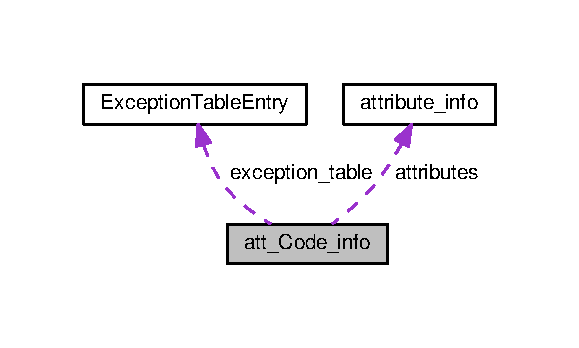
\includegraphics[width=278pt]{structatt__Code__info__coll__graph}
\end{center}
\end{figure}
\subsection*{Data Fields}
\begin{DoxyCompactItemize}
\item 
uint16\+\_\+t \hyperlink{structatt__Code__info_aa2d5de07b8832d1cd18a3e4779348fe3}{max\+\_\+stack}
\item 
uint16\+\_\+t \hyperlink{structatt__Code__info_acc9a5f7316ef5c5e051f88646bacf445}{max\+\_\+locals}
\item 
uint32\+\_\+t \hyperlink{structatt__Code__info_a24832826292dff47147e23f9d440bd2a}{code\+\_\+length}
\item 
uint8\+\_\+t $\ast$ \hyperlink{structatt__Code__info_a8fb8f2fa609ccf1786492efca32d3be9}{code}
\item 
uint16\+\_\+t \hyperlink{structatt__Code__info_aacd07775342d4f5ace7485e36e2e5e3b}{exception\+\_\+table\+\_\+length}
\item 
\hyperlink{structExceptionTableEntry}{Exception\+Table\+Entry} $\ast$ \hyperlink{structatt__Code__info_af5c5d84bb1f725dc949981cc752c45d2}{exception\+\_\+table}
\item 
uint16\+\_\+t \hyperlink{structatt__Code__info_a9bed6599acdfbf0b3391c827272a5502}{attributes\+\_\+count}
\item 
\hyperlink{structattribute__info}{attribute\+\_\+info} $\ast$ \hyperlink{structatt__Code__info_a09d52ef82f22bf27c4b5e3f2ab021f79}{attributes}
\end{DoxyCompactItemize}


\subsection{Field Documentation}
\index{att\+\_\+\+Code\+\_\+info@{att\+\_\+\+Code\+\_\+info}!attributes@{attributes}}
\index{attributes@{attributes}!att\+\_\+\+Code\+\_\+info@{att\+\_\+\+Code\+\_\+info}}
\subsubsection[{\texorpdfstring{attributes}{attributes}}]{\setlength{\rightskip}{0pt plus 5cm}{\bf attribute\+\_\+info}$\ast$ att\+\_\+\+Code\+\_\+info\+::attributes}\hypertarget{structatt__Code__info_a09d52ef82f22bf27c4b5e3f2ab021f79}{}\label{structatt__Code__info_a09d52ef82f22bf27c4b5e3f2ab021f79}
\index{att\+\_\+\+Code\+\_\+info@{att\+\_\+\+Code\+\_\+info}!attributes\+\_\+count@{attributes\+\_\+count}}
\index{attributes\+\_\+count@{attributes\+\_\+count}!att\+\_\+\+Code\+\_\+info@{att\+\_\+\+Code\+\_\+info}}
\subsubsection[{\texorpdfstring{attributes\+\_\+count}{attributes_count}}]{\setlength{\rightskip}{0pt plus 5cm}uint16\+\_\+t att\+\_\+\+Code\+\_\+info\+::attributes\+\_\+count}\hypertarget{structatt__Code__info_a9bed6599acdfbf0b3391c827272a5502}{}\label{structatt__Code__info_a9bed6599acdfbf0b3391c827272a5502}
\index{att\+\_\+\+Code\+\_\+info@{att\+\_\+\+Code\+\_\+info}!code@{code}}
\index{code@{code}!att\+\_\+\+Code\+\_\+info@{att\+\_\+\+Code\+\_\+info}}
\subsubsection[{\texorpdfstring{code}{code}}]{\setlength{\rightskip}{0pt plus 5cm}uint8\+\_\+t$\ast$ att\+\_\+\+Code\+\_\+info\+::code}\hypertarget{structatt__Code__info_a8fb8f2fa609ccf1786492efca32d3be9}{}\label{structatt__Code__info_a8fb8f2fa609ccf1786492efca32d3be9}
\index{att\+\_\+\+Code\+\_\+info@{att\+\_\+\+Code\+\_\+info}!code\+\_\+length@{code\+\_\+length}}
\index{code\+\_\+length@{code\+\_\+length}!att\+\_\+\+Code\+\_\+info@{att\+\_\+\+Code\+\_\+info}}
\subsubsection[{\texorpdfstring{code\+\_\+length}{code_length}}]{\setlength{\rightskip}{0pt plus 5cm}uint32\+\_\+t att\+\_\+\+Code\+\_\+info\+::code\+\_\+length}\hypertarget{structatt__Code__info_a24832826292dff47147e23f9d440bd2a}{}\label{structatt__Code__info_a24832826292dff47147e23f9d440bd2a}
\index{att\+\_\+\+Code\+\_\+info@{att\+\_\+\+Code\+\_\+info}!exception\+\_\+table@{exception\+\_\+table}}
\index{exception\+\_\+table@{exception\+\_\+table}!att\+\_\+\+Code\+\_\+info@{att\+\_\+\+Code\+\_\+info}}
\subsubsection[{\texorpdfstring{exception\+\_\+table}{exception_table}}]{\setlength{\rightskip}{0pt plus 5cm}{\bf Exception\+Table\+Entry}$\ast$ att\+\_\+\+Code\+\_\+info\+::exception\+\_\+table}\hypertarget{structatt__Code__info_af5c5d84bb1f725dc949981cc752c45d2}{}\label{structatt__Code__info_af5c5d84bb1f725dc949981cc752c45d2}
\index{att\+\_\+\+Code\+\_\+info@{att\+\_\+\+Code\+\_\+info}!exception\+\_\+table\+\_\+length@{exception\+\_\+table\+\_\+length}}
\index{exception\+\_\+table\+\_\+length@{exception\+\_\+table\+\_\+length}!att\+\_\+\+Code\+\_\+info@{att\+\_\+\+Code\+\_\+info}}
\subsubsection[{\texorpdfstring{exception\+\_\+table\+\_\+length}{exception_table_length}}]{\setlength{\rightskip}{0pt plus 5cm}uint16\+\_\+t att\+\_\+\+Code\+\_\+info\+::exception\+\_\+table\+\_\+length}\hypertarget{structatt__Code__info_aacd07775342d4f5ace7485e36e2e5e3b}{}\label{structatt__Code__info_aacd07775342d4f5ace7485e36e2e5e3b}
\index{att\+\_\+\+Code\+\_\+info@{att\+\_\+\+Code\+\_\+info}!max\+\_\+locals@{max\+\_\+locals}}
\index{max\+\_\+locals@{max\+\_\+locals}!att\+\_\+\+Code\+\_\+info@{att\+\_\+\+Code\+\_\+info}}
\subsubsection[{\texorpdfstring{max\+\_\+locals}{max_locals}}]{\setlength{\rightskip}{0pt plus 5cm}uint16\+\_\+t att\+\_\+\+Code\+\_\+info\+::max\+\_\+locals}\hypertarget{structatt__Code__info_acc9a5f7316ef5c5e051f88646bacf445}{}\label{structatt__Code__info_acc9a5f7316ef5c5e051f88646bacf445}
\index{att\+\_\+\+Code\+\_\+info@{att\+\_\+\+Code\+\_\+info}!max\+\_\+stack@{max\+\_\+stack}}
\index{max\+\_\+stack@{max\+\_\+stack}!att\+\_\+\+Code\+\_\+info@{att\+\_\+\+Code\+\_\+info}}
\subsubsection[{\texorpdfstring{max\+\_\+stack}{max_stack}}]{\setlength{\rightskip}{0pt plus 5cm}uint16\+\_\+t att\+\_\+\+Code\+\_\+info\+::max\+\_\+stack}\hypertarget{structatt__Code__info_aa2d5de07b8832d1cd18a3e4779348fe3}{}\label{structatt__Code__info_aa2d5de07b8832d1cd18a3e4779348fe3}


The documentation for this struct was generated from the following file\+:\begin{DoxyCompactItemize}
\item 
src/\hyperlink{attributes_8h}{attributes.\+h}\end{DoxyCompactItemize}

\hypertarget{structatt__ConstantValue__info}{}\section{att\+\_\+\+Constant\+Value\+\_\+info Struct Reference}
\label{structatt__ConstantValue__info}\index{att\+\_\+\+Constant\+Value\+\_\+info@{att\+\_\+\+Constant\+Value\+\_\+info}}


{\ttfamily \#include $<$attributes.\+h$>$}

\subsection*{Data Fields}
\begin{DoxyCompactItemize}
\item 
uint16\+\_\+t \hyperlink{structatt__ConstantValue__info_a6d9c6fc03274f8dc77c2ea8c53744dfa}{constantvalue\+\_\+index}
\end{DoxyCompactItemize}


\subsection{Field Documentation}
\index{att\+\_\+\+Constant\+Value\+\_\+info@{att\+\_\+\+Constant\+Value\+\_\+info}!constantvalue\+\_\+index@{constantvalue\+\_\+index}}
\index{constantvalue\+\_\+index@{constantvalue\+\_\+index}!att\+\_\+\+Constant\+Value\+\_\+info@{att\+\_\+\+Constant\+Value\+\_\+info}}
\subsubsection[{\texorpdfstring{constantvalue\+\_\+index}{constantvalue_index}}]{\setlength{\rightskip}{0pt plus 5cm}uint16\+\_\+t att\+\_\+\+Constant\+Value\+\_\+info\+::constantvalue\+\_\+index}\hypertarget{structatt__ConstantValue__info_a6d9c6fc03274f8dc77c2ea8c53744dfa}{}\label{structatt__ConstantValue__info_a6d9c6fc03274f8dc77c2ea8c53744dfa}


The documentation for this struct was generated from the following file\+:\begin{DoxyCompactItemize}
\item 
src/\hyperlink{attributes_8h}{attributes.\+h}\end{DoxyCompactItemize}

\hypertarget{structatt__Exceptions__info}{}\section{att\+\_\+\+Exceptions\+\_\+info Struct Reference}
\label{structatt__Exceptions__info}\index{att\+\_\+\+Exceptions\+\_\+info@{att\+\_\+\+Exceptions\+\_\+info}}


{\ttfamily \#include $<$attributes.\+h$>$}

\subsection*{Data Fields}
\begin{DoxyCompactItemize}
\item 
uint16\+\_\+t \hyperlink{structatt__Exceptions__info_aa118cef845f2ff9472572598b79ef635}{number\+\_\+of\+\_\+exceptions}
\item 
uint16\+\_\+t $\ast$ \hyperlink{structatt__Exceptions__info_ae713b303537b79289f22216ddbcbfd56}{exception\+\_\+index\+\_\+table}
\end{DoxyCompactItemize}


\subsection{Field Documentation}
\index{att\+\_\+\+Exceptions\+\_\+info@{att\+\_\+\+Exceptions\+\_\+info}!exception\+\_\+index\+\_\+table@{exception\+\_\+index\+\_\+table}}
\index{exception\+\_\+index\+\_\+table@{exception\+\_\+index\+\_\+table}!att\+\_\+\+Exceptions\+\_\+info@{att\+\_\+\+Exceptions\+\_\+info}}
\subsubsection[{\texorpdfstring{exception\+\_\+index\+\_\+table}{exception_index_table}}]{\setlength{\rightskip}{0pt plus 5cm}uint16\+\_\+t$\ast$ att\+\_\+\+Exceptions\+\_\+info\+::exception\+\_\+index\+\_\+table}\hypertarget{structatt__Exceptions__info_ae713b303537b79289f22216ddbcbfd56}{}\label{structatt__Exceptions__info_ae713b303537b79289f22216ddbcbfd56}
\index{att\+\_\+\+Exceptions\+\_\+info@{att\+\_\+\+Exceptions\+\_\+info}!number\+\_\+of\+\_\+exceptions@{number\+\_\+of\+\_\+exceptions}}
\index{number\+\_\+of\+\_\+exceptions@{number\+\_\+of\+\_\+exceptions}!att\+\_\+\+Exceptions\+\_\+info@{att\+\_\+\+Exceptions\+\_\+info}}
\subsubsection[{\texorpdfstring{number\+\_\+of\+\_\+exceptions}{number_of_exceptions}}]{\setlength{\rightskip}{0pt plus 5cm}uint16\+\_\+t att\+\_\+\+Exceptions\+\_\+info\+::number\+\_\+of\+\_\+exceptions}\hypertarget{structatt__Exceptions__info_aa118cef845f2ff9472572598b79ef635}{}\label{structatt__Exceptions__info_aa118cef845f2ff9472572598b79ef635}


The documentation for this struct was generated from the following file\+:\begin{DoxyCompactItemize}
\item 
src/\hyperlink{attributes_8h}{attributes.\+h}\end{DoxyCompactItemize}

\hypertarget{structatt__InnerClasses__info}{}\section{att\+\_\+\+Inner\+Classes\+\_\+info Struct Reference}
\label{structatt__InnerClasses__info}\index{att\+\_\+\+Inner\+Classes\+\_\+info@{att\+\_\+\+Inner\+Classes\+\_\+info}}


{\ttfamily \#include $<$attributes.\+h$>$}



Collaboration diagram for att\+\_\+\+Inner\+Classes\+\_\+info\+:\nopagebreak
\begin{figure}[H]
\begin{center}
\leavevmode
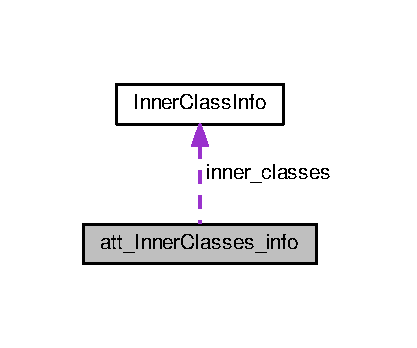
\includegraphics[width=200pt]{structatt__InnerClasses__info__coll__graph}
\end{center}
\end{figure}
\subsection*{Data Fields}
\begin{DoxyCompactItemize}
\item 
uint16\+\_\+t \hyperlink{structatt__InnerClasses__info_a8bb396e50023f850c80a70e0b736cc77}{number\+\_\+of\+\_\+classes}
\item 
\hyperlink{structInnerClassInfo}{Inner\+Class\+Info} $\ast$ \hyperlink{structatt__InnerClasses__info_a68beb2632952ef867172bfcfa327d256}{inner\+\_\+classes}
\end{DoxyCompactItemize}


\subsection{Field Documentation}
\index{att\+\_\+\+Inner\+Classes\+\_\+info@{att\+\_\+\+Inner\+Classes\+\_\+info}!inner\+\_\+classes@{inner\+\_\+classes}}
\index{inner\+\_\+classes@{inner\+\_\+classes}!att\+\_\+\+Inner\+Classes\+\_\+info@{att\+\_\+\+Inner\+Classes\+\_\+info}}
\subsubsection[{\texorpdfstring{inner\+\_\+classes}{inner_classes}}]{\setlength{\rightskip}{0pt plus 5cm}{\bf Inner\+Class\+Info}$\ast$ att\+\_\+\+Inner\+Classes\+\_\+info\+::inner\+\_\+classes}\hypertarget{structatt__InnerClasses__info_a68beb2632952ef867172bfcfa327d256}{}\label{structatt__InnerClasses__info_a68beb2632952ef867172bfcfa327d256}
\index{att\+\_\+\+Inner\+Classes\+\_\+info@{att\+\_\+\+Inner\+Classes\+\_\+info}!number\+\_\+of\+\_\+classes@{number\+\_\+of\+\_\+classes}}
\index{number\+\_\+of\+\_\+classes@{number\+\_\+of\+\_\+classes}!att\+\_\+\+Inner\+Classes\+\_\+info@{att\+\_\+\+Inner\+Classes\+\_\+info}}
\subsubsection[{\texorpdfstring{number\+\_\+of\+\_\+classes}{number_of_classes}}]{\setlength{\rightskip}{0pt plus 5cm}uint16\+\_\+t att\+\_\+\+Inner\+Classes\+\_\+info\+::number\+\_\+of\+\_\+classes}\hypertarget{structatt__InnerClasses__info_a8bb396e50023f850c80a70e0b736cc77}{}\label{structatt__InnerClasses__info_a8bb396e50023f850c80a70e0b736cc77}


The documentation for this struct was generated from the following file\+:\begin{DoxyCompactItemize}
\item 
src/\hyperlink{attributes_8h}{attributes.\+h}\end{DoxyCompactItemize}

\hypertarget{structatt__LineNumberTable__info}{}\section{att\+\_\+\+Line\+Number\+Table\+\_\+info Struct Reference}
\label{structatt__LineNumberTable__info}\index{att\+\_\+\+Line\+Number\+Table\+\_\+info@{att\+\_\+\+Line\+Number\+Table\+\_\+info}}


{\ttfamily \#include $<$attributes.\+h$>$}



Collaboration diagram for att\+\_\+\+Line\+Number\+Table\+\_\+info\+:\nopagebreak
\begin{figure}[H]
\begin{center}
\leavevmode
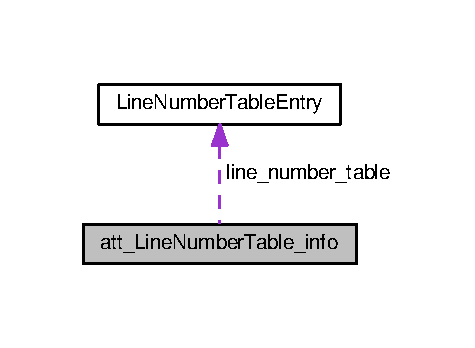
\includegraphics[width=228pt]{structatt__LineNumberTable__info__coll__graph}
\end{center}
\end{figure}
\subsection*{Data Fields}
\begin{DoxyCompactItemize}
\item 
uint16\+\_\+t \hyperlink{structatt__LineNumberTable__info_a6c335e2b6b14577d9a0e063cd5a361e0}{line\+\_\+number\+\_\+table\+\_\+length}
\item 
\hyperlink{structLineNumberTableEntry}{Line\+Number\+Table\+Entry} $\ast$ \hyperlink{structatt__LineNumberTable__info_ac9c52cc4b931ea8cfc746ea0a1d573ac}{line\+\_\+number\+\_\+table}
\end{DoxyCompactItemize}


\subsection{Field Documentation}
\index{att\+\_\+\+Line\+Number\+Table\+\_\+info@{att\+\_\+\+Line\+Number\+Table\+\_\+info}!line\+\_\+number\+\_\+table@{line\+\_\+number\+\_\+table}}
\index{line\+\_\+number\+\_\+table@{line\+\_\+number\+\_\+table}!att\+\_\+\+Line\+Number\+Table\+\_\+info@{att\+\_\+\+Line\+Number\+Table\+\_\+info}}
\subsubsection[{\texorpdfstring{line\+\_\+number\+\_\+table}{line_number_table}}]{\setlength{\rightskip}{0pt plus 5cm}{\bf Line\+Number\+Table\+Entry}$\ast$ att\+\_\+\+Line\+Number\+Table\+\_\+info\+::line\+\_\+number\+\_\+table}\hypertarget{structatt__LineNumberTable__info_ac9c52cc4b931ea8cfc746ea0a1d573ac}{}\label{structatt__LineNumberTable__info_ac9c52cc4b931ea8cfc746ea0a1d573ac}
\index{att\+\_\+\+Line\+Number\+Table\+\_\+info@{att\+\_\+\+Line\+Number\+Table\+\_\+info}!line\+\_\+number\+\_\+table\+\_\+length@{line\+\_\+number\+\_\+table\+\_\+length}}
\index{line\+\_\+number\+\_\+table\+\_\+length@{line\+\_\+number\+\_\+table\+\_\+length}!att\+\_\+\+Line\+Number\+Table\+\_\+info@{att\+\_\+\+Line\+Number\+Table\+\_\+info}}
\subsubsection[{\texorpdfstring{line\+\_\+number\+\_\+table\+\_\+length}{line_number_table_length}}]{\setlength{\rightskip}{0pt plus 5cm}uint16\+\_\+t att\+\_\+\+Line\+Number\+Table\+\_\+info\+::line\+\_\+number\+\_\+table\+\_\+length}\hypertarget{structatt__LineNumberTable__info_a6c335e2b6b14577d9a0e063cd5a361e0}{}\label{structatt__LineNumberTable__info_a6c335e2b6b14577d9a0e063cd5a361e0}


The documentation for this struct was generated from the following file\+:\begin{DoxyCompactItemize}
\item 
src/\hyperlink{attributes_8h}{attributes.\+h}\end{DoxyCompactItemize}

\hypertarget{structatt__SourceFile__info}{}\section{att\+\_\+\+Source\+File\+\_\+info Struct Reference}
\label{structatt__SourceFile__info}\index{att\+\_\+\+Source\+File\+\_\+info@{att\+\_\+\+Source\+File\+\_\+info}}


{\ttfamily \#include $<$attributes.\+h$>$}

\subsection*{Data Fields}
\begin{DoxyCompactItemize}
\item 
uint16\+\_\+t \hyperlink{structatt__SourceFile__info_a8cd88fda3147c1e7b1270dcc39754f1c}{sourcefile\+\_\+index}
\end{DoxyCompactItemize}


\subsection{Field Documentation}
\index{att\+\_\+\+Source\+File\+\_\+info@{att\+\_\+\+Source\+File\+\_\+info}!sourcefile\+\_\+index@{sourcefile\+\_\+index}}
\index{sourcefile\+\_\+index@{sourcefile\+\_\+index}!att\+\_\+\+Source\+File\+\_\+info@{att\+\_\+\+Source\+File\+\_\+info}}
\subsubsection[{\texorpdfstring{sourcefile\+\_\+index}{sourcefile_index}}]{\setlength{\rightskip}{0pt plus 5cm}uint16\+\_\+t att\+\_\+\+Source\+File\+\_\+info\+::sourcefile\+\_\+index}\hypertarget{structatt__SourceFile__info_a8cd88fda3147c1e7b1270dcc39754f1c}{}\label{structatt__SourceFile__info_a8cd88fda3147c1e7b1270dcc39754f1c}


The documentation for this struct was generated from the following file\+:\begin{DoxyCompactItemize}
\item 
src/\hyperlink{attributes_8h}{attributes.\+h}\end{DoxyCompactItemize}

\hypertarget{structattribute__info}{}\section{attribute\+\_\+info Struct Reference}
\label{structattribute__info}\index{attribute\+\_\+info@{attribute\+\_\+info}}


{\ttfamily \#include $<$attributes.\+h$>$}

\subsection*{Data Fields}
\begin{DoxyCompactItemize}
\item 
uint16\+\_\+t \hyperlink{structattribute__info_a7e925cf3d7a72731f1b6a6e4d1c24cc2}{name\+\_\+index}
\item 
uint32\+\_\+t \hyperlink{structattribute__info_a9528b298d46309f571f1f58c84cbd57c}{length}
\item 
void $\ast$ \hyperlink{structattribute__info_a7f168925308e418b7b44c9f11fdf42ae}{info}
\item 
uint8\+\_\+t \hyperlink{structattribute__info_aba7285ff2ef220420c41b51470921544}{attribute\+Type}
\end{DoxyCompactItemize}


\subsection{Field Documentation}
\index{attribute\+\_\+info@{attribute\+\_\+info}!attribute\+Type@{attribute\+Type}}
\index{attribute\+Type@{attribute\+Type}!attribute\+\_\+info@{attribute\+\_\+info}}
\subsubsection[{\texorpdfstring{attribute\+Type}{attributeType}}]{\setlength{\rightskip}{0pt plus 5cm}uint8\+\_\+t attribute\+\_\+info\+::attribute\+Type}\hypertarget{structattribute__info_aba7285ff2ef220420c41b51470921544}{}\label{structattribute__info_aba7285ff2ef220420c41b51470921544}
\index{attribute\+\_\+info@{attribute\+\_\+info}!info@{info}}
\index{info@{info}!attribute\+\_\+info@{attribute\+\_\+info}}
\subsubsection[{\texorpdfstring{info}{info}}]{\setlength{\rightskip}{0pt plus 5cm}void$\ast$ attribute\+\_\+info\+::info}\hypertarget{structattribute__info_a7f168925308e418b7b44c9f11fdf42ae}{}\label{structattribute__info_a7f168925308e418b7b44c9f11fdf42ae}
\index{attribute\+\_\+info@{attribute\+\_\+info}!length@{length}}
\index{length@{length}!attribute\+\_\+info@{attribute\+\_\+info}}
\subsubsection[{\texorpdfstring{length}{length}}]{\setlength{\rightskip}{0pt plus 5cm}uint32\+\_\+t attribute\+\_\+info\+::length}\hypertarget{structattribute__info_a9528b298d46309f571f1f58c84cbd57c}{}\label{structattribute__info_a9528b298d46309f571f1f58c84cbd57c}
\index{attribute\+\_\+info@{attribute\+\_\+info}!name\+\_\+index@{name\+\_\+index}}
\index{name\+\_\+index@{name\+\_\+index}!attribute\+\_\+info@{attribute\+\_\+info}}
\subsubsection[{\texorpdfstring{name\+\_\+index}{name_index}}]{\setlength{\rightskip}{0pt plus 5cm}uint16\+\_\+t attribute\+\_\+info\+::name\+\_\+index}\hypertarget{structattribute__info_a7e925cf3d7a72731f1b6a6e4d1c24cc2}{}\label{structattribute__info_a7e925cf3d7a72731f1b6a6e4d1c24cc2}


The documentation for this struct was generated from the following file\+:\begin{DoxyCompactItemize}
\item 
src/\hyperlink{attributes_8h}{attributes.\+h}\end{DoxyCompactItemize}

\hypertarget{structClassInstance}{}\section{Class\+Instance Struct Reference}
\label{structClassInstance}\index{Class\+Instance@{Class\+Instance}}


{\ttfamily \#include $<$jvm.\+h$>$}



Collaboration diagram for Class\+Instance\+:\nopagebreak
\begin{figure}[H]
\begin{center}
\leavevmode
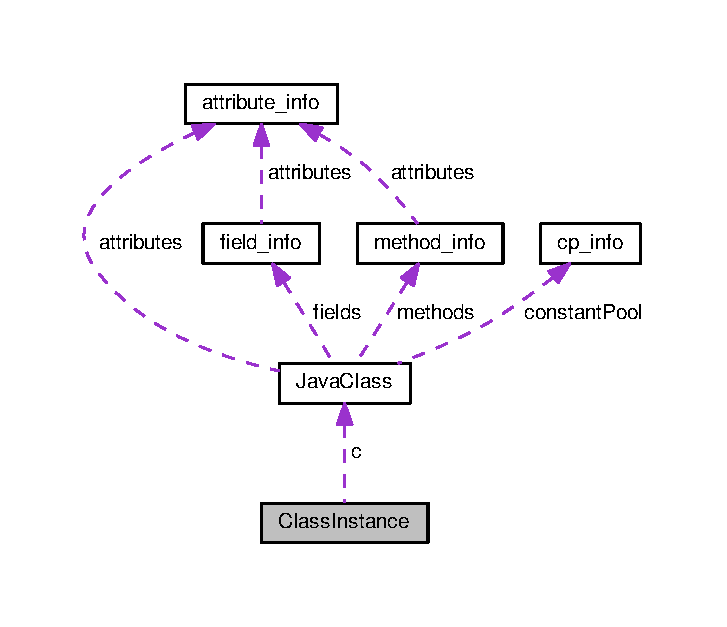
\includegraphics[width=349pt]{structClassInstance__coll__graph}
\end{center}
\end{figure}
\subsection*{Data Fields}
\begin{DoxyCompactItemize}
\item 
\hyperlink{structJavaClass}{Java\+Class} $\ast$ \hyperlink{structClassInstance_a315745fb5b53a63e4c9771c778a05373}{c}
\item 
int32\+\_\+t $\ast$ \hyperlink{structClassInstance_a6096fe53fe197dc9f0642135216ee182}{data}
\end{DoxyCompactItemize}


\subsection{Field Documentation}
\index{Class\+Instance@{Class\+Instance}!c@{c}}
\index{c@{c}!Class\+Instance@{Class\+Instance}}
\subsubsection[{\texorpdfstring{c}{c}}]{\setlength{\rightskip}{0pt plus 5cm}{\bf Java\+Class}$\ast$ Class\+Instance\+::c}\hypertarget{structClassInstance_a315745fb5b53a63e4c9771c778a05373}{}\label{structClassInstance_a315745fb5b53a63e4c9771c778a05373}
\index{Class\+Instance@{Class\+Instance}!data@{data}}
\index{data@{data}!Class\+Instance@{Class\+Instance}}
\subsubsection[{\texorpdfstring{data}{data}}]{\setlength{\rightskip}{0pt plus 5cm}int32\+\_\+t$\ast$ Class\+Instance\+::data}\hypertarget{structClassInstance_a6096fe53fe197dc9f0642135216ee182}{}\label{structClassInstance_a6096fe53fe197dc9f0642135216ee182}


The documentation for this struct was generated from the following file\+:\begin{DoxyCompactItemize}
\item 
src/\hyperlink{jvm_8h}{jvm.\+h}\end{DoxyCompactItemize}

\hypertarget{structcp__info}{}\section{cp\+\_\+info Struct Reference}
\label{structcp__info}\index{cp\+\_\+info@{cp\+\_\+info}}


{\ttfamily \#include $<$constantpool.\+h$>$}

\subsection*{Data Fields}
\begin{DoxyCompactItemize}
\item 
uint8\+\_\+t \hyperlink{structcp__info_a29d87595bc993eb6cd53f30e8305ec74}{tag}
\item 
\begin{tabbing}
xx\=xx\=xx\=xx\=xx\=xx\=xx\=xx\=xx\=\kill
union \{\\
\>struct \{\\
\>\>uint16\_t \hyperlink{structcp__info_a3c8912fe67e7d3f9ce150aa6f5bec22d}{name\_index}\\
\>\} \hyperlink{structcp__info_aeb14fdcb3ba2363a18f2ecbeac15ac41}{Class}\\
\>struct \{\\
\>\>uint16\_t \hyperlink{structcp__info_aa63dfc7668d7eff682f88b09c48eddc8}{string\_index}\\
\>\} \hyperlink{structcp__info_a0e7c2a98e0cf4ffeb32047c7d78d835c}{String}\\
\>struct \{\\
\>\>uint16\_t \hyperlink{structcp__info_ab2b48e96f2178c47f9f6b683c9b2fc59}{class\_index}\\
\>\>uint16\_t \hyperlink{structcp__info_ad7a8733b3b078818a59cc33eb1fa7dc3}{name\_and\_type\_index}\\
\>\} \hyperlink{structcp__info_ac2cdad99f486a8e1bd1a66a06556a945}{Fieldref}\\
\>struct \{\\
\>\>uint16\_t \hyperlink{structcp__info_ab2b48e96f2178c47f9f6b683c9b2fc59}{class\_index}\\
\>\>uint16\_t \hyperlink{structcp__info_ad7a8733b3b078818a59cc33eb1fa7dc3}{name\_and\_type\_index}\\
\>\} \hyperlink{structcp__info_a3a2f2fccc08f122c44a2cd3405ee6264}{Methodref}\\
\>struct \{\\
\>\>uint16\_t \hyperlink{structcp__info_ab2b48e96f2178c47f9f6b683c9b2fc59}{class\_index}\\
\>\>uint16\_t \hyperlink{structcp__info_ad7a8733b3b078818a59cc33eb1fa7dc3}{name\_and\_type\_index}\\
\>\} \hyperlink{structcp__info_aa83f8676e24f088925c6502b78765d04}{InterfaceMethodref}\\
\>struct \{\\
\>\>uint16\_t \hyperlink{structcp__info_a3c8912fe67e7d3f9ce150aa6f5bec22d}{name\_index}\\
\>\>uint16\_t \hyperlink{structcp__info_aef3c90a1a874ca4acbc49029aaa0d4cb}{descriptor\_index}\\
\>\} \hyperlink{structcp__info_a992e807724524d5cdd537a646478e7c3}{NameAndType}\\
\>struct \{\\
\>\>uint32\_t \hyperlink{structcp__info_abdf544fc1b14cb7bfcb5ecabb74a0e84}{value}\\
\>\} \hyperlink{structcp__info_af859585c09920ad4589135731a78e772}{Integer}\\
\>struct \{\\
\>\>uint32\_t \hyperlink{structcp__info_a34ed0f597e452fbeb97cb0f551a678bb}{bytes}\\
\>\} \hyperlink{structcp__info_aa58271cb0f8e9d8827b2e99380f4b777}{Float}\\
\>struct \{\\
\>\>uint32\_t \hyperlink{structcp__info_a73d116220b0d9e7674ab0bd34bcb155a}{high}\\
\>\>uint32\_t \hyperlink{structcp__info_ae325e667e647b781e0691686049e50ec}{low}\\
\>\} \hyperlink{structcp__info_a000e2b8074c512960f81e10a1946ae94}{Long}\\
\>struct \{\\
\>\>uint32\_t \hyperlink{structcp__info_a73d116220b0d9e7674ab0bd34bcb155a}{high}\\
\>\>uint32\_t \hyperlink{structcp__info_ae325e667e647b781e0691686049e50ec}{low}\\
\>\} \hyperlink{structcp__info_aa42214f97b75a51fadba707aa3c29749}{Double}\\
\>struct \{\\
\>\>uint16\_t \hyperlink{structcp__info_afa18d3ff419ce300281ca759a20a2cc3}{length}\\
\>\>uint8\_t $\ast$ \hyperlink{structcp__info_a34c1da9248b884af89b5c91d55087100}{bytes}\\
\>\} \hyperlink{structcp__info_a25ee4592009bd74535de00796abf40eb}{Utf8}\\
\}; \\

\end{tabbing}\end{DoxyCompactItemize}


\subsection{Field Documentation}
\subsubsection[{\texorpdfstring{"@1}{@1}}]{\setlength{\rightskip}{0pt plus 5cm}union \{ ... \} }\hypertarget{structcp__info_ab2df10b8ac24e6e4dc2e383a68c00447}{}\label{structcp__info_ab2df10b8ac24e6e4dc2e383a68c00447}
\index{cp\+\_\+info@{cp\+\_\+info}!bytes@{bytes}}
\index{bytes@{bytes}!cp\+\_\+info@{cp\+\_\+info}}
\subsubsection[{\texorpdfstring{bytes}{bytes}}]{\setlength{\rightskip}{0pt plus 5cm}uint32\+\_\+t cp\+\_\+info\+::bytes}\hypertarget{structcp__info_a34ed0f597e452fbeb97cb0f551a678bb}{}\label{structcp__info_a34ed0f597e452fbeb97cb0f551a678bb}
\index{cp\+\_\+info@{cp\+\_\+info}!bytes@{bytes}}
\index{bytes@{bytes}!cp\+\_\+info@{cp\+\_\+info}}
\subsubsection[{\texorpdfstring{bytes}{bytes}}]{\setlength{\rightskip}{0pt plus 5cm}uint8\+\_\+t$\ast$ cp\+\_\+info\+::bytes}\hypertarget{structcp__info_a34c1da9248b884af89b5c91d55087100}{}\label{structcp__info_a34c1da9248b884af89b5c91d55087100}
\index{cp\+\_\+info@{cp\+\_\+info}!Class@{Class}}
\index{Class@{Class}!cp\+\_\+info@{cp\+\_\+info}}
\subsubsection[{\texorpdfstring{Class}{Class}}]{\setlength{\rightskip}{0pt plus 5cm}struct \{ ... \}   cp\+\_\+info\+::\+Class}\hypertarget{structcp__info_aeb14fdcb3ba2363a18f2ecbeac15ac41}{}\label{structcp__info_aeb14fdcb3ba2363a18f2ecbeac15ac41}
\index{cp\+\_\+info@{cp\+\_\+info}!class\+\_\+index@{class\+\_\+index}}
\index{class\+\_\+index@{class\+\_\+index}!cp\+\_\+info@{cp\+\_\+info}}
\subsubsection[{\texorpdfstring{class\+\_\+index}{class_index}}]{\setlength{\rightskip}{0pt plus 5cm}uint16\+\_\+t cp\+\_\+info\+::class\+\_\+index}\hypertarget{structcp__info_ab2b48e96f2178c47f9f6b683c9b2fc59}{}\label{structcp__info_ab2b48e96f2178c47f9f6b683c9b2fc59}
\index{cp\+\_\+info@{cp\+\_\+info}!descriptor\+\_\+index@{descriptor\+\_\+index}}
\index{descriptor\+\_\+index@{descriptor\+\_\+index}!cp\+\_\+info@{cp\+\_\+info}}
\subsubsection[{\texorpdfstring{descriptor\+\_\+index}{descriptor_index}}]{\setlength{\rightskip}{0pt plus 5cm}uint16\+\_\+t cp\+\_\+info\+::descriptor\+\_\+index}\hypertarget{structcp__info_aef3c90a1a874ca4acbc49029aaa0d4cb}{}\label{structcp__info_aef3c90a1a874ca4acbc49029aaa0d4cb}
\index{cp\+\_\+info@{cp\+\_\+info}!Double@{Double}}
\index{Double@{Double}!cp\+\_\+info@{cp\+\_\+info}}
\subsubsection[{\texorpdfstring{Double}{Double}}]{\setlength{\rightskip}{0pt plus 5cm}struct \{ ... \}   cp\+\_\+info\+::\+Double}\hypertarget{structcp__info_aa42214f97b75a51fadba707aa3c29749}{}\label{structcp__info_aa42214f97b75a51fadba707aa3c29749}
\index{cp\+\_\+info@{cp\+\_\+info}!Fieldref@{Fieldref}}
\index{Fieldref@{Fieldref}!cp\+\_\+info@{cp\+\_\+info}}
\subsubsection[{\texorpdfstring{Fieldref}{Fieldref}}]{\setlength{\rightskip}{0pt plus 5cm}struct \{ ... \}   cp\+\_\+info\+::\+Fieldref}\hypertarget{structcp__info_ac2cdad99f486a8e1bd1a66a06556a945}{}\label{structcp__info_ac2cdad99f486a8e1bd1a66a06556a945}
\index{cp\+\_\+info@{cp\+\_\+info}!Float@{Float}}
\index{Float@{Float}!cp\+\_\+info@{cp\+\_\+info}}
\subsubsection[{\texorpdfstring{Float}{Float}}]{\setlength{\rightskip}{0pt plus 5cm}struct \{ ... \}   cp\+\_\+info\+::\+Float}\hypertarget{structcp__info_aa58271cb0f8e9d8827b2e99380f4b777}{}\label{structcp__info_aa58271cb0f8e9d8827b2e99380f4b777}
\index{cp\+\_\+info@{cp\+\_\+info}!high@{high}}
\index{high@{high}!cp\+\_\+info@{cp\+\_\+info}}
\subsubsection[{\texorpdfstring{high}{high}}]{\setlength{\rightskip}{0pt plus 5cm}uint32\+\_\+t cp\+\_\+info\+::high}\hypertarget{structcp__info_a73d116220b0d9e7674ab0bd34bcb155a}{}\label{structcp__info_a73d116220b0d9e7674ab0bd34bcb155a}
\index{cp\+\_\+info@{cp\+\_\+info}!Integer@{Integer}}
\index{Integer@{Integer}!cp\+\_\+info@{cp\+\_\+info}}
\subsubsection[{\texorpdfstring{Integer}{Integer}}]{\setlength{\rightskip}{0pt plus 5cm}struct \{ ... \}   cp\+\_\+info\+::\+Integer}\hypertarget{structcp__info_af859585c09920ad4589135731a78e772}{}\label{structcp__info_af859585c09920ad4589135731a78e772}
\index{cp\+\_\+info@{cp\+\_\+info}!Interface\+Methodref@{Interface\+Methodref}}
\index{Interface\+Methodref@{Interface\+Methodref}!cp\+\_\+info@{cp\+\_\+info}}
\subsubsection[{\texorpdfstring{Interface\+Methodref}{InterfaceMethodref}}]{\setlength{\rightskip}{0pt plus 5cm}struct \{ ... \}   cp\+\_\+info\+::\+Interface\+Methodref}\hypertarget{structcp__info_aa83f8676e24f088925c6502b78765d04}{}\label{structcp__info_aa83f8676e24f088925c6502b78765d04}
\index{cp\+\_\+info@{cp\+\_\+info}!length@{length}}
\index{length@{length}!cp\+\_\+info@{cp\+\_\+info}}
\subsubsection[{\texorpdfstring{length}{length}}]{\setlength{\rightskip}{0pt plus 5cm}uint16\+\_\+t cp\+\_\+info\+::length}\hypertarget{structcp__info_afa18d3ff419ce300281ca759a20a2cc3}{}\label{structcp__info_afa18d3ff419ce300281ca759a20a2cc3}
\index{cp\+\_\+info@{cp\+\_\+info}!Long@{Long}}
\index{Long@{Long}!cp\+\_\+info@{cp\+\_\+info}}
\subsubsection[{\texorpdfstring{Long}{Long}}]{\setlength{\rightskip}{0pt plus 5cm}struct \{ ... \}   cp\+\_\+info\+::\+Long}\hypertarget{structcp__info_a000e2b8074c512960f81e10a1946ae94}{}\label{structcp__info_a000e2b8074c512960f81e10a1946ae94}
\index{cp\+\_\+info@{cp\+\_\+info}!low@{low}}
\index{low@{low}!cp\+\_\+info@{cp\+\_\+info}}
\subsubsection[{\texorpdfstring{low}{low}}]{\setlength{\rightskip}{0pt plus 5cm}uint32\+\_\+t cp\+\_\+info\+::low}\hypertarget{structcp__info_ae325e667e647b781e0691686049e50ec}{}\label{structcp__info_ae325e667e647b781e0691686049e50ec}
\index{cp\+\_\+info@{cp\+\_\+info}!Methodref@{Methodref}}
\index{Methodref@{Methodref}!cp\+\_\+info@{cp\+\_\+info}}
\subsubsection[{\texorpdfstring{Methodref}{Methodref}}]{\setlength{\rightskip}{0pt plus 5cm}struct \{ ... \}   cp\+\_\+info\+::\+Methodref}\hypertarget{structcp__info_a3a2f2fccc08f122c44a2cd3405ee6264}{}\label{structcp__info_a3a2f2fccc08f122c44a2cd3405ee6264}
\index{cp\+\_\+info@{cp\+\_\+info}!name\+\_\+and\+\_\+type\+\_\+index@{name\+\_\+and\+\_\+type\+\_\+index}}
\index{name\+\_\+and\+\_\+type\+\_\+index@{name\+\_\+and\+\_\+type\+\_\+index}!cp\+\_\+info@{cp\+\_\+info}}
\subsubsection[{\texorpdfstring{name\+\_\+and\+\_\+type\+\_\+index}{name_and_type_index}}]{\setlength{\rightskip}{0pt plus 5cm}uint16\+\_\+t cp\+\_\+info\+::name\+\_\+and\+\_\+type\+\_\+index}\hypertarget{structcp__info_ad7a8733b3b078818a59cc33eb1fa7dc3}{}\label{structcp__info_ad7a8733b3b078818a59cc33eb1fa7dc3}
\index{cp\+\_\+info@{cp\+\_\+info}!name\+\_\+index@{name\+\_\+index}}
\index{name\+\_\+index@{name\+\_\+index}!cp\+\_\+info@{cp\+\_\+info}}
\subsubsection[{\texorpdfstring{name\+\_\+index}{name_index}}]{\setlength{\rightskip}{0pt plus 5cm}uint16\+\_\+t cp\+\_\+info\+::name\+\_\+index}\hypertarget{structcp__info_a3c8912fe67e7d3f9ce150aa6f5bec22d}{}\label{structcp__info_a3c8912fe67e7d3f9ce150aa6f5bec22d}
\index{cp\+\_\+info@{cp\+\_\+info}!Name\+And\+Type@{Name\+And\+Type}}
\index{Name\+And\+Type@{Name\+And\+Type}!cp\+\_\+info@{cp\+\_\+info}}
\subsubsection[{\texorpdfstring{Name\+And\+Type}{NameAndType}}]{\setlength{\rightskip}{0pt plus 5cm}struct \{ ... \}   cp\+\_\+info\+::\+Name\+And\+Type}\hypertarget{structcp__info_a992e807724524d5cdd537a646478e7c3}{}\label{structcp__info_a992e807724524d5cdd537a646478e7c3}
\index{cp\+\_\+info@{cp\+\_\+info}!String@{String}}
\index{String@{String}!cp\+\_\+info@{cp\+\_\+info}}
\subsubsection[{\texorpdfstring{String}{String}}]{\setlength{\rightskip}{0pt plus 5cm}struct \{ ... \}   cp\+\_\+info\+::\+String}\hypertarget{structcp__info_a0e7c2a98e0cf4ffeb32047c7d78d835c}{}\label{structcp__info_a0e7c2a98e0cf4ffeb32047c7d78d835c}
\index{cp\+\_\+info@{cp\+\_\+info}!string\+\_\+index@{string\+\_\+index}}
\index{string\+\_\+index@{string\+\_\+index}!cp\+\_\+info@{cp\+\_\+info}}
\subsubsection[{\texorpdfstring{string\+\_\+index}{string_index}}]{\setlength{\rightskip}{0pt plus 5cm}uint16\+\_\+t cp\+\_\+info\+::string\+\_\+index}\hypertarget{structcp__info_aa63dfc7668d7eff682f88b09c48eddc8}{}\label{structcp__info_aa63dfc7668d7eff682f88b09c48eddc8}
\index{cp\+\_\+info@{cp\+\_\+info}!tag@{tag}}
\index{tag@{tag}!cp\+\_\+info@{cp\+\_\+info}}
\subsubsection[{\texorpdfstring{tag}{tag}}]{\setlength{\rightskip}{0pt plus 5cm}uint8\+\_\+t cp\+\_\+info\+::tag}\hypertarget{structcp__info_a29d87595bc993eb6cd53f30e8305ec74}{}\label{structcp__info_a29d87595bc993eb6cd53f30e8305ec74}
\index{cp\+\_\+info@{cp\+\_\+info}!Utf8@{Utf8}}
\index{Utf8@{Utf8}!cp\+\_\+info@{cp\+\_\+info}}
\subsubsection[{\texorpdfstring{Utf8}{Utf8}}]{\setlength{\rightskip}{0pt plus 5cm}struct \{ ... \}   cp\+\_\+info\+::\+Utf8}\hypertarget{structcp__info_a25ee4592009bd74535de00796abf40eb}{}\label{structcp__info_a25ee4592009bd74535de00796abf40eb}
\index{cp\+\_\+info@{cp\+\_\+info}!value@{value}}
\index{value@{value}!cp\+\_\+info@{cp\+\_\+info}}
\subsubsection[{\texorpdfstring{value}{value}}]{\setlength{\rightskip}{0pt plus 5cm}uint32\+\_\+t cp\+\_\+info\+::value}\hypertarget{structcp__info_abdf544fc1b14cb7bfcb5ecabb74a0e84}{}\label{structcp__info_abdf544fc1b14cb7bfcb5ecabb74a0e84}


The documentation for this struct was generated from the following file\+:\begin{DoxyCompactItemize}
\item 
src/\hyperlink{constantpool_8h}{constantpool.\+h}\end{DoxyCompactItemize}

\hypertarget{structExceptionTableEntry}{}\section{Exception\+Table\+Entry Struct Reference}
\label{structExceptionTableEntry}\index{Exception\+Table\+Entry@{Exception\+Table\+Entry}}


{\ttfamily \#include $<$attributes.\+h$>$}

\subsection*{Data Fields}
\begin{DoxyCompactItemize}
\item 
uint16\+\_\+t \hyperlink{structExceptionTableEntry_a2b590ee5474b087686f851f10e3f8f06}{start\+\_\+pc}
\item 
uint16\+\_\+t \hyperlink{structExceptionTableEntry_a876e2f736b1b5f4f081ce96b2923f23e}{end\+\_\+pc}
\item 
uint16\+\_\+t \hyperlink{structExceptionTableEntry_a3fd0ed5cca1781e941594ef0af475add}{handler\+\_\+pc}
\item 
uint16\+\_\+t \hyperlink{structExceptionTableEntry_a7c5ab5cc44557c2e4b92c4643683205d}{catch\+\_\+type}
\end{DoxyCompactItemize}


\subsection{Field Documentation}
\index{Exception\+Table\+Entry@{Exception\+Table\+Entry}!catch\+\_\+type@{catch\+\_\+type}}
\index{catch\+\_\+type@{catch\+\_\+type}!Exception\+Table\+Entry@{Exception\+Table\+Entry}}
\subsubsection[{\texorpdfstring{catch\+\_\+type}{catch_type}}]{\setlength{\rightskip}{0pt plus 5cm}uint16\+\_\+t Exception\+Table\+Entry\+::catch\+\_\+type}\hypertarget{structExceptionTableEntry_a7c5ab5cc44557c2e4b92c4643683205d}{}\label{structExceptionTableEntry_a7c5ab5cc44557c2e4b92c4643683205d}
\index{Exception\+Table\+Entry@{Exception\+Table\+Entry}!end\+\_\+pc@{end\+\_\+pc}}
\index{end\+\_\+pc@{end\+\_\+pc}!Exception\+Table\+Entry@{Exception\+Table\+Entry}}
\subsubsection[{\texorpdfstring{end\+\_\+pc}{end_pc}}]{\setlength{\rightskip}{0pt plus 5cm}uint16\+\_\+t Exception\+Table\+Entry\+::end\+\_\+pc}\hypertarget{structExceptionTableEntry_a876e2f736b1b5f4f081ce96b2923f23e}{}\label{structExceptionTableEntry_a876e2f736b1b5f4f081ce96b2923f23e}
\index{Exception\+Table\+Entry@{Exception\+Table\+Entry}!handler\+\_\+pc@{handler\+\_\+pc}}
\index{handler\+\_\+pc@{handler\+\_\+pc}!Exception\+Table\+Entry@{Exception\+Table\+Entry}}
\subsubsection[{\texorpdfstring{handler\+\_\+pc}{handler_pc}}]{\setlength{\rightskip}{0pt plus 5cm}uint16\+\_\+t Exception\+Table\+Entry\+::handler\+\_\+pc}\hypertarget{structExceptionTableEntry_a3fd0ed5cca1781e941594ef0af475add}{}\label{structExceptionTableEntry_a3fd0ed5cca1781e941594ef0af475add}
\index{Exception\+Table\+Entry@{Exception\+Table\+Entry}!start\+\_\+pc@{start\+\_\+pc}}
\index{start\+\_\+pc@{start\+\_\+pc}!Exception\+Table\+Entry@{Exception\+Table\+Entry}}
\subsubsection[{\texorpdfstring{start\+\_\+pc}{start_pc}}]{\setlength{\rightskip}{0pt plus 5cm}uint16\+\_\+t Exception\+Table\+Entry\+::start\+\_\+pc}\hypertarget{structExceptionTableEntry_a2b590ee5474b087686f851f10e3f8f06}{}\label{structExceptionTableEntry_a2b590ee5474b087686f851f10e3f8f06}


The documentation for this struct was generated from the following file\+:\begin{DoxyCompactItemize}
\item 
src/\hyperlink{attributes_8h}{attributes.\+h}\end{DoxyCompactItemize}

\hypertarget{structfield__info}{}\section{field\+\_\+info Struct Reference}
\label{structfield__info}\index{field\+\_\+info@{field\+\_\+info}}


{\ttfamily \#include $<$fields.\+h$>$}



Collaboration diagram for field\+\_\+info\+:\nopagebreak
\begin{figure}[H]
\begin{center}
\leavevmode
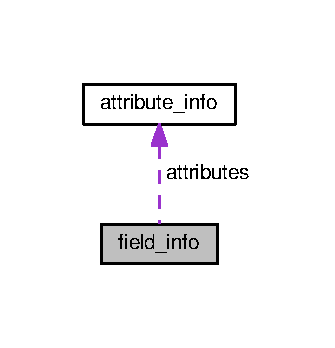
\includegraphics[width=161pt]{structfield__info__coll__graph}
\end{center}
\end{figure}
\subsection*{Data Fields}
\begin{DoxyCompactItemize}
\item 
uint16\+\_\+t \hyperlink{structfield__info_a97bcc8f6647cee71ea02bdd4183ba1da}{access\+\_\+flags}
\item 
uint16\+\_\+t \hyperlink{structfield__info_a3041f6a85347269c5253f7d377384b06}{name\+\_\+index}
\item 
uint16\+\_\+t \hyperlink{structfield__info_a56345eae0135047540b60ca34c91eb46}{descriptor\+\_\+index}
\item 
uint16\+\_\+t \hyperlink{structfield__info_a26aebef0abc97afef9e9a34701e6b550}{attributes\+\_\+count}
\item 
\hyperlink{structattribute__info}{attribute\+\_\+info} $\ast$ \hyperlink{structfield__info_afdda114944ae5eaae78c237f99257108}{attributes}
\item 
uint16\+\_\+t \hyperlink{structfield__info_ad6febfc2078ae2a35339d57079a28b3d}{offset}
\end{DoxyCompactItemize}


\subsection{Field Documentation}
\index{field\+\_\+info@{field\+\_\+info}!access\+\_\+flags@{access\+\_\+flags}}
\index{access\+\_\+flags@{access\+\_\+flags}!field\+\_\+info@{field\+\_\+info}}
\subsubsection[{\texorpdfstring{access\+\_\+flags}{access_flags}}]{\setlength{\rightskip}{0pt plus 5cm}uint16\+\_\+t field\+\_\+info\+::access\+\_\+flags}\hypertarget{structfield__info_a97bcc8f6647cee71ea02bdd4183ba1da}{}\label{structfield__info_a97bcc8f6647cee71ea02bdd4183ba1da}
\index{field\+\_\+info@{field\+\_\+info}!attributes@{attributes}}
\index{attributes@{attributes}!field\+\_\+info@{field\+\_\+info}}
\subsubsection[{\texorpdfstring{attributes}{attributes}}]{\setlength{\rightskip}{0pt plus 5cm}{\bf attribute\+\_\+info}$\ast$ field\+\_\+info\+::attributes}\hypertarget{structfield__info_afdda114944ae5eaae78c237f99257108}{}\label{structfield__info_afdda114944ae5eaae78c237f99257108}
\index{field\+\_\+info@{field\+\_\+info}!attributes\+\_\+count@{attributes\+\_\+count}}
\index{attributes\+\_\+count@{attributes\+\_\+count}!field\+\_\+info@{field\+\_\+info}}
\subsubsection[{\texorpdfstring{attributes\+\_\+count}{attributes_count}}]{\setlength{\rightskip}{0pt plus 5cm}uint16\+\_\+t field\+\_\+info\+::attributes\+\_\+count}\hypertarget{structfield__info_a26aebef0abc97afef9e9a34701e6b550}{}\label{structfield__info_a26aebef0abc97afef9e9a34701e6b550}
\index{field\+\_\+info@{field\+\_\+info}!descriptor\+\_\+index@{descriptor\+\_\+index}}
\index{descriptor\+\_\+index@{descriptor\+\_\+index}!field\+\_\+info@{field\+\_\+info}}
\subsubsection[{\texorpdfstring{descriptor\+\_\+index}{descriptor_index}}]{\setlength{\rightskip}{0pt plus 5cm}uint16\+\_\+t field\+\_\+info\+::descriptor\+\_\+index}\hypertarget{structfield__info_a56345eae0135047540b60ca34c91eb46}{}\label{structfield__info_a56345eae0135047540b60ca34c91eb46}
\index{field\+\_\+info@{field\+\_\+info}!name\+\_\+index@{name\+\_\+index}}
\index{name\+\_\+index@{name\+\_\+index}!field\+\_\+info@{field\+\_\+info}}
\subsubsection[{\texorpdfstring{name\+\_\+index}{name_index}}]{\setlength{\rightskip}{0pt plus 5cm}uint16\+\_\+t field\+\_\+info\+::name\+\_\+index}\hypertarget{structfield__info_a3041f6a85347269c5253f7d377384b06}{}\label{structfield__info_a3041f6a85347269c5253f7d377384b06}
\index{field\+\_\+info@{field\+\_\+info}!offset@{offset}}
\index{offset@{offset}!field\+\_\+info@{field\+\_\+info}}
\subsubsection[{\texorpdfstring{offset}{offset}}]{\setlength{\rightskip}{0pt plus 5cm}uint16\+\_\+t field\+\_\+info\+::offset}\hypertarget{structfield__info_ad6febfc2078ae2a35339d57079a28b3d}{}\label{structfield__info_ad6febfc2078ae2a35339d57079a28b3d}


The documentation for this struct was generated from the following file\+:\begin{DoxyCompactItemize}
\item 
src/\hyperlink{fields_8h}{fields.\+h}\end{DoxyCompactItemize}

\hypertarget{structFrame}{}\section{Frame Struct Reference}
\label{structFrame}\index{Frame@{Frame}}


{\ttfamily \#include $<$framestack.\+h$>$}



Collaboration diagram for Frame\+:\nopagebreak
\begin{figure}[H]
\begin{center}
\leavevmode
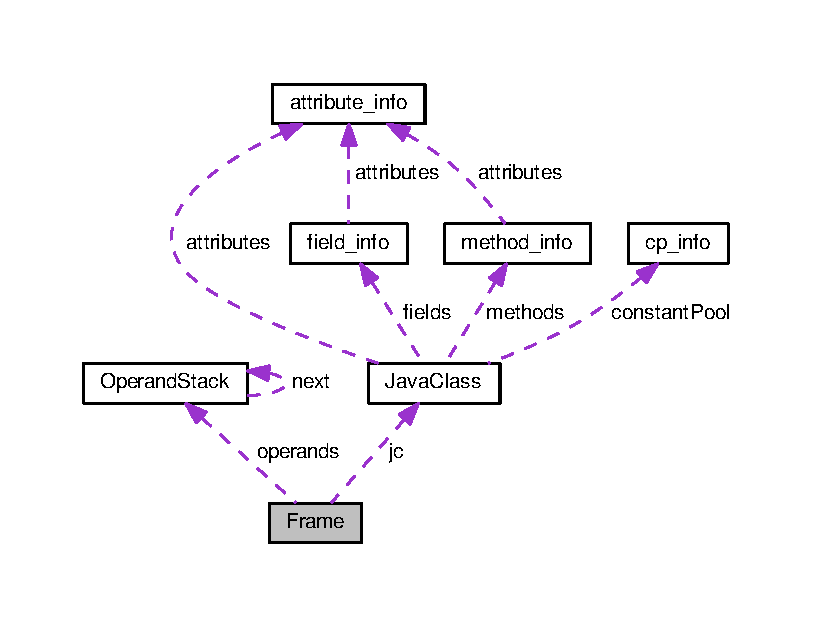
\includegraphics[width=350pt]{structFrame__coll__graph}
\end{center}
\end{figure}
\subsection*{Data Fields}
\begin{DoxyCompactItemize}
\item 
\hyperlink{structJavaClass}{Java\+Class} $\ast$ \hyperlink{structFrame_a6a053c391bc6b65491e72d2fc8ef360f}{jc}
\item 
uint8\+\_\+t \hyperlink{structFrame_ab031c9459d085013efbd0bd3b6a6da34}{fp\+\_\+strict}
\item 
uint8\+\_\+t \hyperlink{structFrame_aa5732143b7e6cc091fc23a3222364ed0}{return\+Count}
\item 
uint32\+\_\+t \hyperlink{structFrame_a91e50d2091184efb52b6d7c0c21fd4b2}{pc}
\item 
uint32\+\_\+t \hyperlink{structFrame_a33a0dd3a739e1dcfd8b03621c752bb28}{code\+\_\+length}
\item 
uint8\+\_\+t $\ast$ \hyperlink{structFrame_a9de8be272246d00c7a0c2ddc899fe8f2}{code}
\item 
\hyperlink{structOperandStack}{Operand\+Stack} $\ast$ \hyperlink{structFrame_a0be587b8515083ff6d3c4e55918a7657}{operands}
\item 
int32\+\_\+t $\ast$ \hyperlink{structFrame_a9047c9524d44fc81cb6311de8a2a8b77}{local\+Variables}
\end{DoxyCompactItemize}


\subsection{Field Documentation}
\index{Frame@{Frame}!code@{code}}
\index{code@{code}!Frame@{Frame}}
\subsubsection[{\texorpdfstring{code}{code}}]{\setlength{\rightskip}{0pt plus 5cm}uint8\+\_\+t$\ast$ Frame\+::code}\hypertarget{structFrame_a9de8be272246d00c7a0c2ddc899fe8f2}{}\label{structFrame_a9de8be272246d00c7a0c2ddc899fe8f2}
\index{Frame@{Frame}!code\+\_\+length@{code\+\_\+length}}
\index{code\+\_\+length@{code\+\_\+length}!Frame@{Frame}}
\subsubsection[{\texorpdfstring{code\+\_\+length}{code_length}}]{\setlength{\rightskip}{0pt plus 5cm}uint32\+\_\+t Frame\+::code\+\_\+length}\hypertarget{structFrame_a33a0dd3a739e1dcfd8b03621c752bb28}{}\label{structFrame_a33a0dd3a739e1dcfd8b03621c752bb28}
\index{Frame@{Frame}!fp\+\_\+strict@{fp\+\_\+strict}}
\index{fp\+\_\+strict@{fp\+\_\+strict}!Frame@{Frame}}
\subsubsection[{\texorpdfstring{fp\+\_\+strict}{fp_strict}}]{\setlength{\rightskip}{0pt plus 5cm}uint8\+\_\+t Frame\+::fp\+\_\+strict}\hypertarget{structFrame_ab031c9459d085013efbd0bd3b6a6da34}{}\label{structFrame_ab031c9459d085013efbd0bd3b6a6da34}
\index{Frame@{Frame}!jc@{jc}}
\index{jc@{jc}!Frame@{Frame}}
\subsubsection[{\texorpdfstring{jc}{jc}}]{\setlength{\rightskip}{0pt plus 5cm}{\bf Java\+Class}$\ast$ Frame\+::jc}\hypertarget{structFrame_a6a053c391bc6b65491e72d2fc8ef360f}{}\label{structFrame_a6a053c391bc6b65491e72d2fc8ef360f}
\index{Frame@{Frame}!local\+Variables@{local\+Variables}}
\index{local\+Variables@{local\+Variables}!Frame@{Frame}}
\subsubsection[{\texorpdfstring{local\+Variables}{localVariables}}]{\setlength{\rightskip}{0pt plus 5cm}int32\+\_\+t$\ast$ Frame\+::local\+Variables}\hypertarget{structFrame_a9047c9524d44fc81cb6311de8a2a8b77}{}\label{structFrame_a9047c9524d44fc81cb6311de8a2a8b77}
\index{Frame@{Frame}!operands@{operands}}
\index{operands@{operands}!Frame@{Frame}}
\subsubsection[{\texorpdfstring{operands}{operands}}]{\setlength{\rightskip}{0pt plus 5cm}{\bf Operand\+Stack}$\ast$ Frame\+::operands}\hypertarget{structFrame_a0be587b8515083ff6d3c4e55918a7657}{}\label{structFrame_a0be587b8515083ff6d3c4e55918a7657}
\index{Frame@{Frame}!pc@{pc}}
\index{pc@{pc}!Frame@{Frame}}
\subsubsection[{\texorpdfstring{pc}{pc}}]{\setlength{\rightskip}{0pt plus 5cm}uint32\+\_\+t Frame\+::pc}\hypertarget{structFrame_a91e50d2091184efb52b6d7c0c21fd4b2}{}\label{structFrame_a91e50d2091184efb52b6d7c0c21fd4b2}
\index{Frame@{Frame}!return\+Count@{return\+Count}}
\index{return\+Count@{return\+Count}!Frame@{Frame}}
\subsubsection[{\texorpdfstring{return\+Count}{returnCount}}]{\setlength{\rightskip}{0pt plus 5cm}uint8\+\_\+t Frame\+::return\+Count}\hypertarget{structFrame_aa5732143b7e6cc091fc23a3222364ed0}{}\label{structFrame_aa5732143b7e6cc091fc23a3222364ed0}


The documentation for this struct was generated from the following file\+:\begin{DoxyCompactItemize}
\item 
src/\hyperlink{framestack_8h}{framestack.\+h}\end{DoxyCompactItemize}

\hypertarget{structFrameStack}{}\section{Frame\+Stack Struct Reference}
\label{structFrameStack}\index{Frame\+Stack@{Frame\+Stack}}


{\ttfamily \#include $<$framestack.\+h$>$}



Collaboration diagram for Frame\+Stack\+:\nopagebreak
\begin{figure}[H]
\begin{center}
\leavevmode
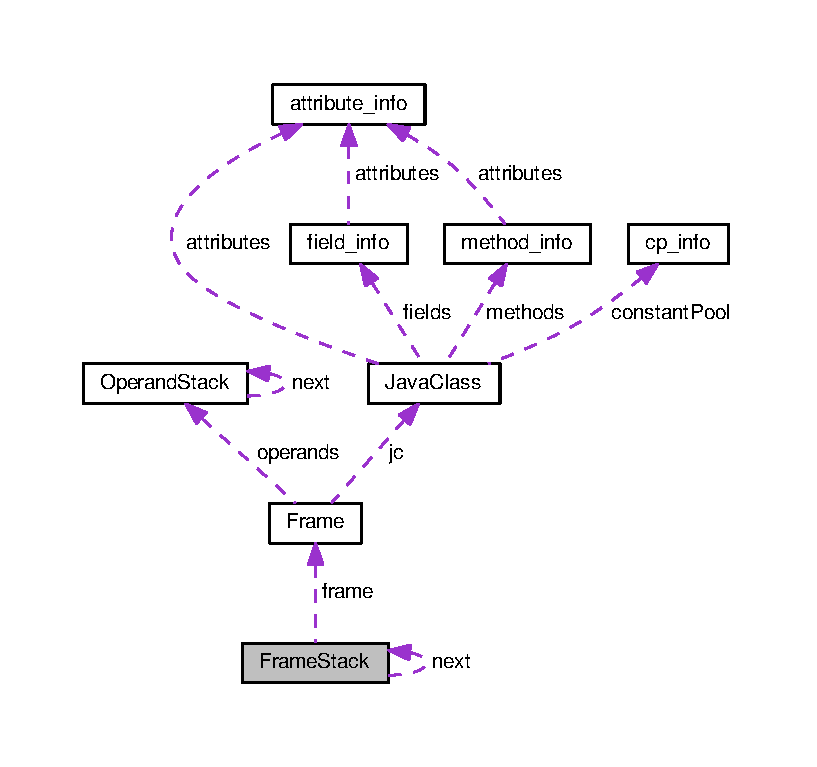
\includegraphics[width=350pt]{structFrameStack__coll__graph}
\end{center}
\end{figure}
\subsection*{Data Fields}
\begin{DoxyCompactItemize}
\item 
\hyperlink{structFrame}{Frame} $\ast$ \hyperlink{structFrameStack_a6175986505277602d1e3cdc9fbbfb8b4}{frame}
\item 
struct \hyperlink{structFrameStack}{Frame\+Stack} $\ast$ \hyperlink{structFrameStack_a7b333d40fd3fda54503169413dec8ddd}{next}
\end{DoxyCompactItemize}


\subsection{Field Documentation}
\index{Frame\+Stack@{Frame\+Stack}!frame@{frame}}
\index{frame@{frame}!Frame\+Stack@{Frame\+Stack}}
\subsubsection[{\texorpdfstring{frame}{frame}}]{\setlength{\rightskip}{0pt plus 5cm}{\bf Frame}$\ast$ Frame\+Stack\+::frame}\hypertarget{structFrameStack_a6175986505277602d1e3cdc9fbbfb8b4}{}\label{structFrameStack_a6175986505277602d1e3cdc9fbbfb8b4}
\index{Frame\+Stack@{Frame\+Stack}!next@{next}}
\index{next@{next}!Frame\+Stack@{Frame\+Stack}}
\subsubsection[{\texorpdfstring{next}{next}}]{\setlength{\rightskip}{0pt plus 5cm}struct {\bf Frame\+Stack}$\ast$ Frame\+Stack\+::next}\hypertarget{structFrameStack_a7b333d40fd3fda54503169413dec8ddd}{}\label{structFrameStack_a7b333d40fd3fda54503169413dec8ddd}


The documentation for this struct was generated from the following file\+:\begin{DoxyCompactItemize}
\item 
src/\hyperlink{framestack_8h}{framestack.\+h}\end{DoxyCompactItemize}

\hypertarget{structInnerClassInfo}{}\section{Inner\+Class\+Info Struct Reference}
\label{structInnerClassInfo}\index{Inner\+Class\+Info@{Inner\+Class\+Info}}


{\ttfamily \#include $<$attributes.\+h$>$}

\subsection*{Data Fields}
\begin{DoxyCompactItemize}
\item 
uint16\+\_\+t \hyperlink{structInnerClassInfo_a3383bc5bea2999b6bd91b9dfc095264f}{inner\+\_\+class\+\_\+index}
\item 
uint16\+\_\+t \hyperlink{structInnerClassInfo_a8449c27dc3cac6e437f4e1c1132ea229}{outer\+\_\+class\+\_\+index}
\item 
uint16\+\_\+t \hyperlink{structInnerClassInfo_a6d008047cb2df8aa856666169f625026}{inner\+\_\+class\+\_\+name\+\_\+index}
\item 
uint16\+\_\+t \hyperlink{structInnerClassInfo_a3810439736cc7ad5cdd1d2cb7aa7c885}{inner\+\_\+class\+\_\+access\+\_\+flags}
\end{DoxyCompactItemize}


\subsection{Field Documentation}
\index{Inner\+Class\+Info@{Inner\+Class\+Info}!inner\+\_\+class\+\_\+access\+\_\+flags@{inner\+\_\+class\+\_\+access\+\_\+flags}}
\index{inner\+\_\+class\+\_\+access\+\_\+flags@{inner\+\_\+class\+\_\+access\+\_\+flags}!Inner\+Class\+Info@{Inner\+Class\+Info}}
\subsubsection[{\texorpdfstring{inner\+\_\+class\+\_\+access\+\_\+flags}{inner_class_access_flags}}]{\setlength{\rightskip}{0pt plus 5cm}uint16\+\_\+t Inner\+Class\+Info\+::inner\+\_\+class\+\_\+access\+\_\+flags}\hypertarget{structInnerClassInfo_a3810439736cc7ad5cdd1d2cb7aa7c885}{}\label{structInnerClassInfo_a3810439736cc7ad5cdd1d2cb7aa7c885}
\index{Inner\+Class\+Info@{Inner\+Class\+Info}!inner\+\_\+class\+\_\+index@{inner\+\_\+class\+\_\+index}}
\index{inner\+\_\+class\+\_\+index@{inner\+\_\+class\+\_\+index}!Inner\+Class\+Info@{Inner\+Class\+Info}}
\subsubsection[{\texorpdfstring{inner\+\_\+class\+\_\+index}{inner_class_index}}]{\setlength{\rightskip}{0pt plus 5cm}uint16\+\_\+t Inner\+Class\+Info\+::inner\+\_\+class\+\_\+index}\hypertarget{structInnerClassInfo_a3383bc5bea2999b6bd91b9dfc095264f}{}\label{structInnerClassInfo_a3383bc5bea2999b6bd91b9dfc095264f}
\index{Inner\+Class\+Info@{Inner\+Class\+Info}!inner\+\_\+class\+\_\+name\+\_\+index@{inner\+\_\+class\+\_\+name\+\_\+index}}
\index{inner\+\_\+class\+\_\+name\+\_\+index@{inner\+\_\+class\+\_\+name\+\_\+index}!Inner\+Class\+Info@{Inner\+Class\+Info}}
\subsubsection[{\texorpdfstring{inner\+\_\+class\+\_\+name\+\_\+index}{inner_class_name_index}}]{\setlength{\rightskip}{0pt plus 5cm}uint16\+\_\+t Inner\+Class\+Info\+::inner\+\_\+class\+\_\+name\+\_\+index}\hypertarget{structInnerClassInfo_a6d008047cb2df8aa856666169f625026}{}\label{structInnerClassInfo_a6d008047cb2df8aa856666169f625026}
\index{Inner\+Class\+Info@{Inner\+Class\+Info}!outer\+\_\+class\+\_\+index@{outer\+\_\+class\+\_\+index}}
\index{outer\+\_\+class\+\_\+index@{outer\+\_\+class\+\_\+index}!Inner\+Class\+Info@{Inner\+Class\+Info}}
\subsubsection[{\texorpdfstring{outer\+\_\+class\+\_\+index}{outer_class_index}}]{\setlength{\rightskip}{0pt plus 5cm}uint16\+\_\+t Inner\+Class\+Info\+::outer\+\_\+class\+\_\+index}\hypertarget{structInnerClassInfo_a8449c27dc3cac6e437f4e1c1132ea229}{}\label{structInnerClassInfo_a8449c27dc3cac6e437f4e1c1132ea229}


The documentation for this struct was generated from the following file\+:\begin{DoxyCompactItemize}
\item 
src/\hyperlink{attributes_8h}{attributes.\+h}\end{DoxyCompactItemize}

\hypertarget{structJavaClass}{}\section{Java\+Class Struct Reference}
\label{structJavaClass}\index{Java\+Class@{Java\+Class}}


{\ttfamily \#include $<$javaclass.\+h$>$}



Collaboration diagram for Java\+Class\+:\nopagebreak
\begin{figure}[H]
\begin{center}
\leavevmode
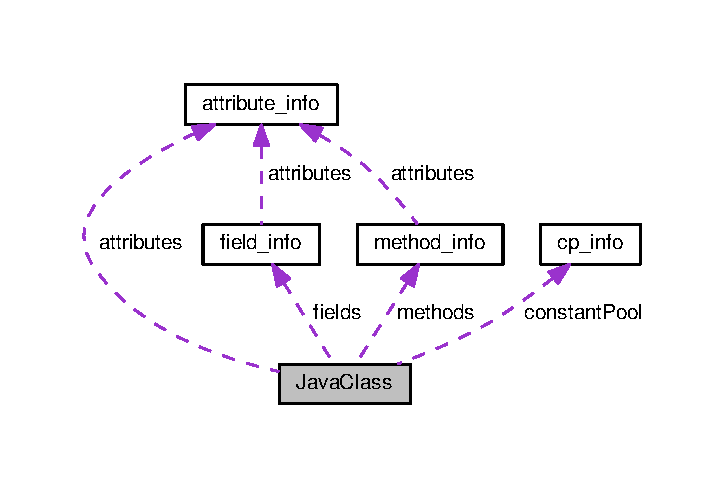
\includegraphics[width=349pt]{structJavaClass__coll__graph}
\end{center}
\end{figure}
\subsection*{Data Fields}
\begin{DoxyCompactItemize}
\item 
F\+I\+LE $\ast$ \hyperlink{structJavaClass_a24301fe0d812773595ca16c4ee658318}{file}
\item 
enum \hyperlink{javaclass_8h_a9b332e6330d199c30e246d4ad8bff5ac}{Java\+Class\+Status} \hyperlink{structJavaClass_aba868ba95744ed4200bd5bba1ad31ffc}{status}
\item 
uint8\+\_\+t \hyperlink{structJavaClass_ae51618e3eb35bfce4a1267d57a686259}{class\+Name\+Mismatch}
\item 
uint16\+\_\+t \hyperlink{structJavaClass_a3961e984041068a78fa5b45414a94a00}{minor\+Version}
\item 
uint16\+\_\+t \hyperlink{structJavaClass_a7e6bc5cab0ffc5091e940cdb3b63e4eb}{major\+Version}
\item 
uint16\+\_\+t \hyperlink{structJavaClass_a89731a6218fb65b228ee1e056c368628}{constant\+Pool\+Count}
\item 
\hyperlink{structcp__info}{cp\+\_\+info} $\ast$ \hyperlink{structJavaClass_ad56dc000ce07c5c6ef57a1ef6f4859e0}{constant\+Pool}
\item 
uint16\+\_\+t \hyperlink{structJavaClass_a305af686b39aafe8248cb4b5af0f5ad4}{access\+Flags}
\item 
uint16\+\_\+t \hyperlink{structJavaClass_ac9af41263ddeabcfafd6464fd82c736f}{this\+Class}
\item 
uint16\+\_\+t \hyperlink{structJavaClass_a08240a259178c4576a82c688f4d3f8a8}{super\+Class}
\item 
uint16\+\_\+t \hyperlink{structJavaClass_a0abfb912729bc17c129e5460ae02dcd3}{interface\+Count}
\item 
uint16\+\_\+t $\ast$ \hyperlink{structJavaClass_a582289dae1229db46bbb8d733edf6a0a}{interfaces}
\item 
uint16\+\_\+t \hyperlink{structJavaClass_ac1568f2faaa136f0877d8a2962c00626}{field\+Count}
\item 
\hyperlink{structfield__info}{field\+\_\+info} $\ast$ \hyperlink{structJavaClass_a84f183bb9d29d499a5e910b9041acd14}{fields}
\item 
uint16\+\_\+t \hyperlink{structJavaClass_a4451678a1ac1921ddb929aced262d1d9}{method\+Count}
\item 
\hyperlink{structmethod__info}{method\+\_\+info} $\ast$ \hyperlink{structJavaClass_ab923c8f31c71ce1602ca21576a48bcb8}{methods}
\item 
uint16\+\_\+t \hyperlink{structJavaClass_ad04e4bd9744078e4f1f739f51295480e}{attribute\+Count}
\item 
\hyperlink{structattribute__info}{attribute\+\_\+info} $\ast$ \hyperlink{structJavaClass_ae90496c9f9b340ef216b24359cb2ff63}{attributes}
\item 
uint16\+\_\+t \hyperlink{structJavaClass_a8b68d0b90dc8af53c6417299b05de8fa}{static\+Field\+Count}
\item 
uint16\+\_\+t \hyperlink{structJavaClass_a5233749f35d2fa0853123ed3ac7ff0c8}{instance\+Field\+Count}
\item 
uint32\+\_\+t \hyperlink{structJavaClass_a58b471dbb758d2a3c1bbd6e0e90fb6e2}{total\+Bytes\+Read}
\item 
uint8\+\_\+t \hyperlink{structJavaClass_a57b0443668351c7380e3d8cdb3e97d7d}{last\+Tag\+Read}
\item 
int32\+\_\+t \hyperlink{structJavaClass_a7e50281e01408da883645af7d983570c}{constant\+Pool\+Entries\+Read}
\item 
int32\+\_\+t \hyperlink{structJavaClass_a4638a5373f392eaaf80048856cb39033}{interface\+Entries\+Read}
\item 
int32\+\_\+t \hyperlink{structJavaClass_a1d9b1e10d762f2153926f46b83180c23}{field\+Entries\+Read}
\item 
int32\+\_\+t \hyperlink{structJavaClass_a5369bcdeb6b25d30dc02df99bf0f0656}{method\+Entries\+Read}
\item 
int32\+\_\+t \hyperlink{structJavaClass_aefcb0a0fbf6d98692680922792d74401}{attribute\+Entries\+Read}
\item 
int32\+\_\+t \hyperlink{structJavaClass_a60729716eb3da22f5517b877343be076}{validity\+Entries\+Checked}
\end{DoxyCompactItemize}


\subsection{Field Documentation}
\index{Java\+Class@{Java\+Class}!access\+Flags@{access\+Flags}}
\index{access\+Flags@{access\+Flags}!Java\+Class@{Java\+Class}}
\subsubsection[{\texorpdfstring{access\+Flags}{accessFlags}}]{\setlength{\rightskip}{0pt plus 5cm}uint16\+\_\+t Java\+Class\+::access\+Flags}\hypertarget{structJavaClass_a305af686b39aafe8248cb4b5af0f5ad4}{}\label{structJavaClass_a305af686b39aafe8248cb4b5af0f5ad4}
\index{Java\+Class@{Java\+Class}!attribute\+Count@{attribute\+Count}}
\index{attribute\+Count@{attribute\+Count}!Java\+Class@{Java\+Class}}
\subsubsection[{\texorpdfstring{attribute\+Count}{attributeCount}}]{\setlength{\rightskip}{0pt plus 5cm}uint16\+\_\+t Java\+Class\+::attribute\+Count}\hypertarget{structJavaClass_ad04e4bd9744078e4f1f739f51295480e}{}\label{structJavaClass_ad04e4bd9744078e4f1f739f51295480e}
\index{Java\+Class@{Java\+Class}!attribute\+Entries\+Read@{attribute\+Entries\+Read}}
\index{attribute\+Entries\+Read@{attribute\+Entries\+Read}!Java\+Class@{Java\+Class}}
\subsubsection[{\texorpdfstring{attribute\+Entries\+Read}{attributeEntriesRead}}]{\setlength{\rightskip}{0pt plus 5cm}int32\+\_\+t Java\+Class\+::attribute\+Entries\+Read}\hypertarget{structJavaClass_aefcb0a0fbf6d98692680922792d74401}{}\label{structJavaClass_aefcb0a0fbf6d98692680922792d74401}
\index{Java\+Class@{Java\+Class}!attributes@{attributes}}
\index{attributes@{attributes}!Java\+Class@{Java\+Class}}
\subsubsection[{\texorpdfstring{attributes}{attributes}}]{\setlength{\rightskip}{0pt plus 5cm}{\bf attribute\+\_\+info}$\ast$ Java\+Class\+::attributes}\hypertarget{structJavaClass_ae90496c9f9b340ef216b24359cb2ff63}{}\label{structJavaClass_ae90496c9f9b340ef216b24359cb2ff63}
\index{Java\+Class@{Java\+Class}!class\+Name\+Mismatch@{class\+Name\+Mismatch}}
\index{class\+Name\+Mismatch@{class\+Name\+Mismatch}!Java\+Class@{Java\+Class}}
\subsubsection[{\texorpdfstring{class\+Name\+Mismatch}{classNameMismatch}}]{\setlength{\rightskip}{0pt plus 5cm}uint8\+\_\+t Java\+Class\+::class\+Name\+Mismatch}\hypertarget{structJavaClass_ae51618e3eb35bfce4a1267d57a686259}{}\label{structJavaClass_ae51618e3eb35bfce4a1267d57a686259}
\index{Java\+Class@{Java\+Class}!constant\+Pool@{constant\+Pool}}
\index{constant\+Pool@{constant\+Pool}!Java\+Class@{Java\+Class}}
\subsubsection[{\texorpdfstring{constant\+Pool}{constantPool}}]{\setlength{\rightskip}{0pt plus 5cm}{\bf cp\+\_\+info}$\ast$ Java\+Class\+::constant\+Pool}\hypertarget{structJavaClass_ad56dc000ce07c5c6ef57a1ef6f4859e0}{}\label{structJavaClass_ad56dc000ce07c5c6ef57a1ef6f4859e0}
\index{Java\+Class@{Java\+Class}!constant\+Pool\+Count@{constant\+Pool\+Count}}
\index{constant\+Pool\+Count@{constant\+Pool\+Count}!Java\+Class@{Java\+Class}}
\subsubsection[{\texorpdfstring{constant\+Pool\+Count}{constantPoolCount}}]{\setlength{\rightskip}{0pt plus 5cm}uint16\+\_\+t Java\+Class\+::constant\+Pool\+Count}\hypertarget{structJavaClass_a89731a6218fb65b228ee1e056c368628}{}\label{structJavaClass_a89731a6218fb65b228ee1e056c368628}
\index{Java\+Class@{Java\+Class}!constant\+Pool\+Entries\+Read@{constant\+Pool\+Entries\+Read}}
\index{constant\+Pool\+Entries\+Read@{constant\+Pool\+Entries\+Read}!Java\+Class@{Java\+Class}}
\subsubsection[{\texorpdfstring{constant\+Pool\+Entries\+Read}{constantPoolEntriesRead}}]{\setlength{\rightskip}{0pt plus 5cm}int32\+\_\+t Java\+Class\+::constant\+Pool\+Entries\+Read}\hypertarget{structJavaClass_a7e50281e01408da883645af7d983570c}{}\label{structJavaClass_a7e50281e01408da883645af7d983570c}
\index{Java\+Class@{Java\+Class}!field\+Count@{field\+Count}}
\index{field\+Count@{field\+Count}!Java\+Class@{Java\+Class}}
\subsubsection[{\texorpdfstring{field\+Count}{fieldCount}}]{\setlength{\rightskip}{0pt plus 5cm}uint16\+\_\+t Java\+Class\+::field\+Count}\hypertarget{structJavaClass_ac1568f2faaa136f0877d8a2962c00626}{}\label{structJavaClass_ac1568f2faaa136f0877d8a2962c00626}
\index{Java\+Class@{Java\+Class}!field\+Entries\+Read@{field\+Entries\+Read}}
\index{field\+Entries\+Read@{field\+Entries\+Read}!Java\+Class@{Java\+Class}}
\subsubsection[{\texorpdfstring{field\+Entries\+Read}{fieldEntriesRead}}]{\setlength{\rightskip}{0pt plus 5cm}int32\+\_\+t Java\+Class\+::field\+Entries\+Read}\hypertarget{structJavaClass_a1d9b1e10d762f2153926f46b83180c23}{}\label{structJavaClass_a1d9b1e10d762f2153926f46b83180c23}
\index{Java\+Class@{Java\+Class}!fields@{fields}}
\index{fields@{fields}!Java\+Class@{Java\+Class}}
\subsubsection[{\texorpdfstring{fields}{fields}}]{\setlength{\rightskip}{0pt plus 5cm}{\bf field\+\_\+info}$\ast$ Java\+Class\+::fields}\hypertarget{structJavaClass_a84f183bb9d29d499a5e910b9041acd14}{}\label{structJavaClass_a84f183bb9d29d499a5e910b9041acd14}
\index{Java\+Class@{Java\+Class}!file@{file}}
\index{file@{file}!Java\+Class@{Java\+Class}}
\subsubsection[{\texorpdfstring{file}{file}}]{\setlength{\rightskip}{0pt plus 5cm}F\+I\+LE$\ast$ Java\+Class\+::file}\hypertarget{structJavaClass_a24301fe0d812773595ca16c4ee658318}{}\label{structJavaClass_a24301fe0d812773595ca16c4ee658318}
\index{Java\+Class@{Java\+Class}!instance\+Field\+Count@{instance\+Field\+Count}}
\index{instance\+Field\+Count@{instance\+Field\+Count}!Java\+Class@{Java\+Class}}
\subsubsection[{\texorpdfstring{instance\+Field\+Count}{instanceFieldCount}}]{\setlength{\rightskip}{0pt plus 5cm}uint16\+\_\+t Java\+Class\+::instance\+Field\+Count}\hypertarget{structJavaClass_a5233749f35d2fa0853123ed3ac7ff0c8}{}\label{structJavaClass_a5233749f35d2fa0853123ed3ac7ff0c8}
\index{Java\+Class@{Java\+Class}!interface\+Count@{interface\+Count}}
\index{interface\+Count@{interface\+Count}!Java\+Class@{Java\+Class}}
\subsubsection[{\texorpdfstring{interface\+Count}{interfaceCount}}]{\setlength{\rightskip}{0pt plus 5cm}uint16\+\_\+t Java\+Class\+::interface\+Count}\hypertarget{structJavaClass_a0abfb912729bc17c129e5460ae02dcd3}{}\label{structJavaClass_a0abfb912729bc17c129e5460ae02dcd3}
\index{Java\+Class@{Java\+Class}!interface\+Entries\+Read@{interface\+Entries\+Read}}
\index{interface\+Entries\+Read@{interface\+Entries\+Read}!Java\+Class@{Java\+Class}}
\subsubsection[{\texorpdfstring{interface\+Entries\+Read}{interfaceEntriesRead}}]{\setlength{\rightskip}{0pt plus 5cm}int32\+\_\+t Java\+Class\+::interface\+Entries\+Read}\hypertarget{structJavaClass_a4638a5373f392eaaf80048856cb39033}{}\label{structJavaClass_a4638a5373f392eaaf80048856cb39033}
\index{Java\+Class@{Java\+Class}!interfaces@{interfaces}}
\index{interfaces@{interfaces}!Java\+Class@{Java\+Class}}
\subsubsection[{\texorpdfstring{interfaces}{interfaces}}]{\setlength{\rightskip}{0pt plus 5cm}uint16\+\_\+t$\ast$ Java\+Class\+::interfaces}\hypertarget{structJavaClass_a582289dae1229db46bbb8d733edf6a0a}{}\label{structJavaClass_a582289dae1229db46bbb8d733edf6a0a}
\index{Java\+Class@{Java\+Class}!last\+Tag\+Read@{last\+Tag\+Read}}
\index{last\+Tag\+Read@{last\+Tag\+Read}!Java\+Class@{Java\+Class}}
\subsubsection[{\texorpdfstring{last\+Tag\+Read}{lastTagRead}}]{\setlength{\rightskip}{0pt plus 5cm}uint8\+\_\+t Java\+Class\+::last\+Tag\+Read}\hypertarget{structJavaClass_a57b0443668351c7380e3d8cdb3e97d7d}{}\label{structJavaClass_a57b0443668351c7380e3d8cdb3e97d7d}
\index{Java\+Class@{Java\+Class}!major\+Version@{major\+Version}}
\index{major\+Version@{major\+Version}!Java\+Class@{Java\+Class}}
\subsubsection[{\texorpdfstring{major\+Version}{majorVersion}}]{\setlength{\rightskip}{0pt plus 5cm}uint16\+\_\+t Java\+Class\+::major\+Version}\hypertarget{structJavaClass_a7e6bc5cab0ffc5091e940cdb3b63e4eb}{}\label{structJavaClass_a7e6bc5cab0ffc5091e940cdb3b63e4eb}
\index{Java\+Class@{Java\+Class}!method\+Count@{method\+Count}}
\index{method\+Count@{method\+Count}!Java\+Class@{Java\+Class}}
\subsubsection[{\texorpdfstring{method\+Count}{methodCount}}]{\setlength{\rightskip}{0pt plus 5cm}uint16\+\_\+t Java\+Class\+::method\+Count}\hypertarget{structJavaClass_a4451678a1ac1921ddb929aced262d1d9}{}\label{structJavaClass_a4451678a1ac1921ddb929aced262d1d9}
\index{Java\+Class@{Java\+Class}!method\+Entries\+Read@{method\+Entries\+Read}}
\index{method\+Entries\+Read@{method\+Entries\+Read}!Java\+Class@{Java\+Class}}
\subsubsection[{\texorpdfstring{method\+Entries\+Read}{methodEntriesRead}}]{\setlength{\rightskip}{0pt plus 5cm}int32\+\_\+t Java\+Class\+::method\+Entries\+Read}\hypertarget{structJavaClass_a5369bcdeb6b25d30dc02df99bf0f0656}{}\label{structJavaClass_a5369bcdeb6b25d30dc02df99bf0f0656}
\index{Java\+Class@{Java\+Class}!methods@{methods}}
\index{methods@{methods}!Java\+Class@{Java\+Class}}
\subsubsection[{\texorpdfstring{methods}{methods}}]{\setlength{\rightskip}{0pt plus 5cm}{\bf method\+\_\+info}$\ast$ Java\+Class\+::methods}\hypertarget{structJavaClass_ab923c8f31c71ce1602ca21576a48bcb8}{}\label{structJavaClass_ab923c8f31c71ce1602ca21576a48bcb8}
\index{Java\+Class@{Java\+Class}!minor\+Version@{minor\+Version}}
\index{minor\+Version@{minor\+Version}!Java\+Class@{Java\+Class}}
\subsubsection[{\texorpdfstring{minor\+Version}{minorVersion}}]{\setlength{\rightskip}{0pt plus 5cm}uint16\+\_\+t Java\+Class\+::minor\+Version}\hypertarget{structJavaClass_a3961e984041068a78fa5b45414a94a00}{}\label{structJavaClass_a3961e984041068a78fa5b45414a94a00}
\index{Java\+Class@{Java\+Class}!static\+Field\+Count@{static\+Field\+Count}}
\index{static\+Field\+Count@{static\+Field\+Count}!Java\+Class@{Java\+Class}}
\subsubsection[{\texorpdfstring{static\+Field\+Count}{staticFieldCount}}]{\setlength{\rightskip}{0pt plus 5cm}uint16\+\_\+t Java\+Class\+::static\+Field\+Count}\hypertarget{structJavaClass_a8b68d0b90dc8af53c6417299b05de8fa}{}\label{structJavaClass_a8b68d0b90dc8af53c6417299b05de8fa}
\index{Java\+Class@{Java\+Class}!status@{status}}
\index{status@{status}!Java\+Class@{Java\+Class}}
\subsubsection[{\texorpdfstring{status}{status}}]{\setlength{\rightskip}{0pt plus 5cm}enum {\bf Java\+Class\+Status} Java\+Class\+::status}\hypertarget{structJavaClass_aba868ba95744ed4200bd5bba1ad31ffc}{}\label{structJavaClass_aba868ba95744ed4200bd5bba1ad31ffc}
\index{Java\+Class@{Java\+Class}!super\+Class@{super\+Class}}
\index{super\+Class@{super\+Class}!Java\+Class@{Java\+Class}}
\subsubsection[{\texorpdfstring{super\+Class}{superClass}}]{\setlength{\rightskip}{0pt plus 5cm}uint16\+\_\+t Java\+Class\+::super\+Class}\hypertarget{structJavaClass_a08240a259178c4576a82c688f4d3f8a8}{}\label{structJavaClass_a08240a259178c4576a82c688f4d3f8a8}
\index{Java\+Class@{Java\+Class}!this\+Class@{this\+Class}}
\index{this\+Class@{this\+Class}!Java\+Class@{Java\+Class}}
\subsubsection[{\texorpdfstring{this\+Class}{thisClass}}]{\setlength{\rightskip}{0pt plus 5cm}uint16\+\_\+t Java\+Class\+::this\+Class}\hypertarget{structJavaClass_ac9af41263ddeabcfafd6464fd82c736f}{}\label{structJavaClass_ac9af41263ddeabcfafd6464fd82c736f}
\index{Java\+Class@{Java\+Class}!total\+Bytes\+Read@{total\+Bytes\+Read}}
\index{total\+Bytes\+Read@{total\+Bytes\+Read}!Java\+Class@{Java\+Class}}
\subsubsection[{\texorpdfstring{total\+Bytes\+Read}{totalBytesRead}}]{\setlength{\rightskip}{0pt plus 5cm}uint32\+\_\+t Java\+Class\+::total\+Bytes\+Read}\hypertarget{structJavaClass_a58b471dbb758d2a3c1bbd6e0e90fb6e2}{}\label{structJavaClass_a58b471dbb758d2a3c1bbd6e0e90fb6e2}
\index{Java\+Class@{Java\+Class}!validity\+Entries\+Checked@{validity\+Entries\+Checked}}
\index{validity\+Entries\+Checked@{validity\+Entries\+Checked}!Java\+Class@{Java\+Class}}
\subsubsection[{\texorpdfstring{validity\+Entries\+Checked}{validityEntriesChecked}}]{\setlength{\rightskip}{0pt plus 5cm}int32\+\_\+t Java\+Class\+::validity\+Entries\+Checked}\hypertarget{structJavaClass_a60729716eb3da22f5517b877343be076}{}\label{structJavaClass_a60729716eb3da22f5517b877343be076}


The documentation for this struct was generated from the following file\+:\begin{DoxyCompactItemize}
\item 
src/\hyperlink{javaclass_8h}{javaclass.\+h}\end{DoxyCompactItemize}

\hypertarget{structJavaVirtualMachine}{}\section{Java\+Virtual\+Machine Struct Reference}
\label{structJavaVirtualMachine}\index{Java\+Virtual\+Machine@{Java\+Virtual\+Machine}}


A java virtual machine, storing all loaded classes, created objects and frames for methods being executed.  




{\ttfamily \#include $<$jvm.\+h$>$}



Collaboration diagram for Java\+Virtual\+Machine\+:\nopagebreak
\begin{figure}[H]
\begin{center}
\leavevmode
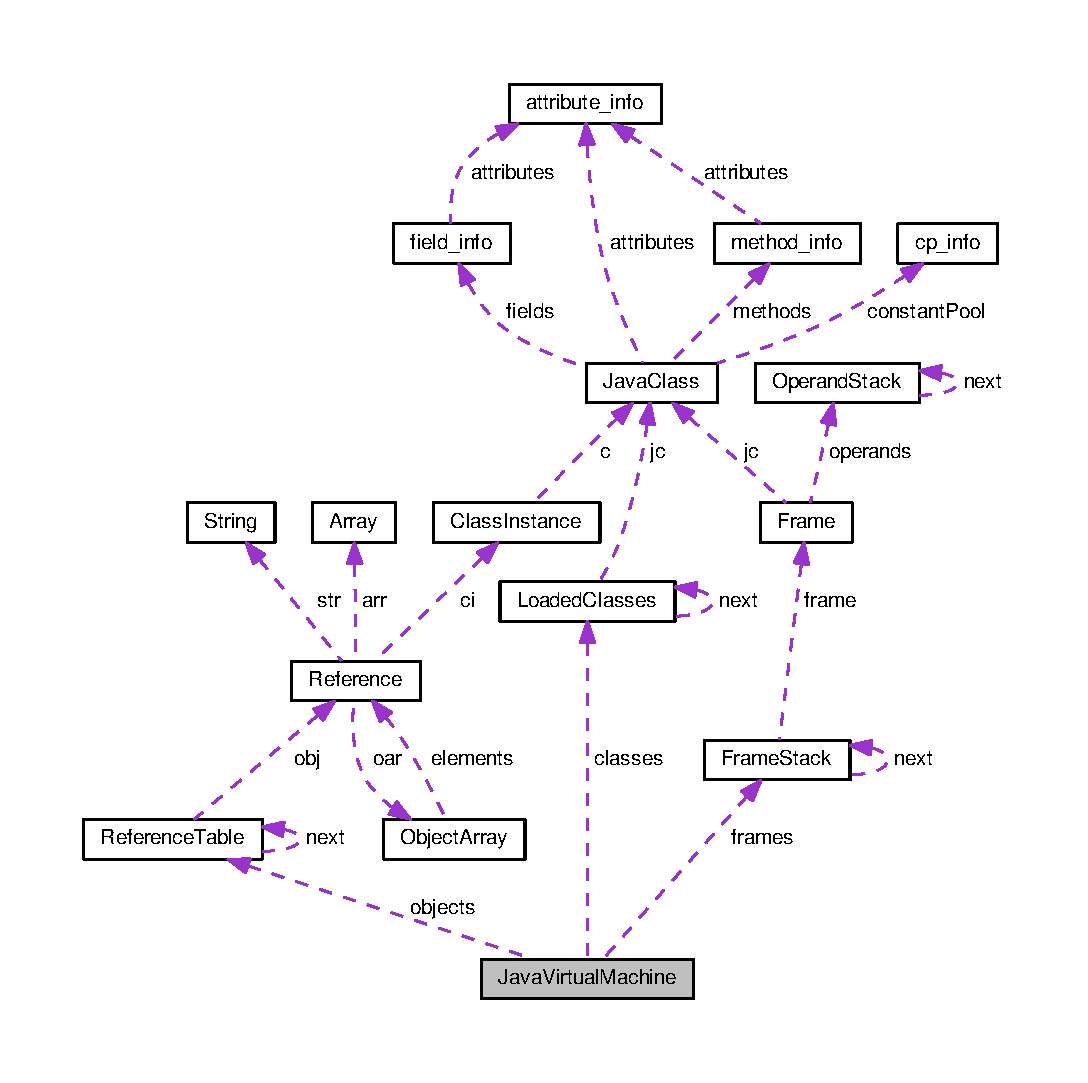
\includegraphics[width=350pt]{structJavaVirtualMachine__coll__graph}
\end{center}
\end{figure}
\subsection*{Data Fields}
\begin{DoxyCompactItemize}
\item 
uint8\+\_\+t \hyperlink{structJavaVirtualMachine_ae8571f20c0db273c88a5ce2d52d51a04}{status}
\begin{DoxyCompactList}\small\item\em Status of the execution of the J\+VM, indicating whether there are errors or not. \end{DoxyCompactList}\item 
uint8\+\_\+t \hyperlink{structJavaVirtualMachine_a98897bec4e614dd62c3d5b1543efd57d}{simulating\+System\+And\+String\+Classes}
\begin{DoxyCompactList}\small\item\em Boolean telling if the System/\+String classes are to be simulated instead of being loaded from their actual .class files. \end{DoxyCompactList}\item 
\hyperlink{structReferenceTable}{Reference\+Table} $\ast$ \hyperlink{structJavaVirtualMachine_a7513525a761cf3172a0ed080cafcee06}{objects}
\begin{DoxyCompactList}\small\item\em Linked list of all objects that have been created during the execution of the J\+VM. \end{DoxyCompactList}\item 
\hyperlink{structFrameStack}{Frame\+Stack} $\ast$ \hyperlink{structJavaVirtualMachine_a6a0d723bb649fabc57742221b01b3617}{frames}
\begin{DoxyCompactList}\small\item\em Stack of all frames created by method calls. \end{DoxyCompactList}\item 
\hyperlink{structLoadedClasses}{Loaded\+Classes} $\ast$ \hyperlink{structJavaVirtualMachine_a36266aec8ba9d25b4d9f67509967dd4c}{classes}
\begin{DoxyCompactList}\small\item\em Linked list containing all classes that have been resolved by the J\+VM. \end{DoxyCompactList}\item 
char \hyperlink{structJavaVirtualMachine_a62e35894409c262231bcae405b4e291b}{class\+Path} \mbox{[}256\mbox{]}
\begin{DoxyCompactList}\small\item\em Path to look for files when opening classes. \end{DoxyCompactList}\end{DoxyCompactItemize}


\subsection{Detailed Description}
A java virtual machine, storing all loaded classes, created objects and frames for methods being executed. 

\begin{DoxySeeAlso}{See also}
\hyperlink{jvm_8c_aca189885e78ec25ece5d7f70e83022a1}{init\+J\+V\+M()}, \hyperlink{jvm_8c_a38b6a19996260e30af5a369a9588dc31}{execute\+J\+V\+M()}, \hyperlink{jvm_8c_a65269d70951aacfe829c89c078dad67a}{deinit\+J\+V\+M()} 
\end{DoxySeeAlso}


\subsection{Field Documentation}
\index{Java\+Virtual\+Machine@{Java\+Virtual\+Machine}!classes@{classes}}
\index{classes@{classes}!Java\+Virtual\+Machine@{Java\+Virtual\+Machine}}
\subsubsection[{\texorpdfstring{classes}{classes}}]{\setlength{\rightskip}{0pt plus 5cm}{\bf Loaded\+Classes}$\ast$ Java\+Virtual\+Machine\+::classes}\hypertarget{structJavaVirtualMachine_a36266aec8ba9d25b4d9f67509967dd4c}{}\label{structJavaVirtualMachine_a36266aec8ba9d25b4d9f67509967dd4c}


Linked list containing all classes that have been resolved by the J\+VM. 

\index{Java\+Virtual\+Machine@{Java\+Virtual\+Machine}!class\+Path@{class\+Path}}
\index{class\+Path@{class\+Path}!Java\+Virtual\+Machine@{Java\+Virtual\+Machine}}
\subsubsection[{\texorpdfstring{class\+Path}{classPath}}]{\setlength{\rightskip}{0pt plus 5cm}char Java\+Virtual\+Machine\+::class\+Path\mbox{[}256\mbox{]}}\hypertarget{structJavaVirtualMachine_a62e35894409c262231bcae405b4e291b}{}\label{structJavaVirtualMachine_a62e35894409c262231bcae405b4e291b}


Path to look for files when opening classes. 

If an attempt to open a class file in the current directory fails, then this class\+Path is used to build another directory to look for the class file. \index{Java\+Virtual\+Machine@{Java\+Virtual\+Machine}!frames@{frames}}
\index{frames@{frames}!Java\+Virtual\+Machine@{Java\+Virtual\+Machine}}
\subsubsection[{\texorpdfstring{frames}{frames}}]{\setlength{\rightskip}{0pt plus 5cm}{\bf Frame\+Stack}$\ast$ Java\+Virtual\+Machine\+::frames}\hypertarget{structJavaVirtualMachine_a6a0d723bb649fabc57742221b01b3617}{}\label{structJavaVirtualMachine_a6a0d723bb649fabc57742221b01b3617}


Stack of all frames created by method calls. 

\index{Java\+Virtual\+Machine@{Java\+Virtual\+Machine}!objects@{objects}}
\index{objects@{objects}!Java\+Virtual\+Machine@{Java\+Virtual\+Machine}}
\subsubsection[{\texorpdfstring{objects}{objects}}]{\setlength{\rightskip}{0pt plus 5cm}{\bf Reference\+Table}$\ast$ Java\+Virtual\+Machine\+::objects}\hypertarget{structJavaVirtualMachine_a7513525a761cf3172a0ed080cafcee06}{}\label{structJavaVirtualMachine_a7513525a761cf3172a0ed080cafcee06}


Linked list of all objects that have been created during the execution of the J\+VM. 

\index{Java\+Virtual\+Machine@{Java\+Virtual\+Machine}!simulating\+System\+And\+String\+Classes@{simulating\+System\+And\+String\+Classes}}
\index{simulating\+System\+And\+String\+Classes@{simulating\+System\+And\+String\+Classes}!Java\+Virtual\+Machine@{Java\+Virtual\+Machine}}
\subsubsection[{\texorpdfstring{simulating\+System\+And\+String\+Classes}{simulatingSystemAndStringClasses}}]{\setlength{\rightskip}{0pt plus 5cm}uint8\+\_\+t Java\+Virtual\+Machine\+::simulating\+System\+And\+String\+Classes}\hypertarget{structJavaVirtualMachine_a98897bec4e614dd62c3d5b1543efd57d}{}\label{structJavaVirtualMachine_a98897bec4e614dd62c3d5b1543efd57d}


Boolean telling if the System/\+String classes are to be simulated instead of being loaded from their actual .class files. 

\begin{DoxyNote}{Note}
Currently it is always set to true, and the support for those classes is minimum. 
\end{DoxyNote}
\index{Java\+Virtual\+Machine@{Java\+Virtual\+Machine}!status@{status}}
\index{status@{status}!Java\+Virtual\+Machine@{Java\+Virtual\+Machine}}
\subsubsection[{\texorpdfstring{status}{status}}]{\setlength{\rightskip}{0pt plus 5cm}uint8\+\_\+t Java\+Virtual\+Machine\+::status}\hypertarget{structJavaVirtualMachine_ae8571f20c0db273c88a5ce2d52d51a04}{}\label{structJavaVirtualMachine_ae8571f20c0db273c88a5ce2d52d51a04}


Status of the execution of the J\+VM, indicating whether there are errors or not. 



The documentation for this struct was generated from the following file\+:\begin{DoxyCompactItemize}
\item 
src/\hyperlink{jvm_8h}{jvm.\+h}\end{DoxyCompactItemize}

\hypertarget{structLineNumberTableEntry}{}\section{Line\+Number\+Table\+Entry Struct Reference}
\label{structLineNumberTableEntry}\index{Line\+Number\+Table\+Entry@{Line\+Number\+Table\+Entry}}


{\ttfamily \#include $<$attributes.\+h$>$}

\subsection*{Data Fields}
\begin{DoxyCompactItemize}
\item 
uint16\+\_\+t \hyperlink{structLineNumberTableEntry_a85d30a6f76c8e89a3358b15e2c6597d4}{start\+\_\+pc}
\item 
uint16\+\_\+t \hyperlink{structLineNumberTableEntry_a1fc3df29fa0ec197a90eb50002a20f9a}{line\+\_\+number}
\end{DoxyCompactItemize}


\subsection{Field Documentation}
\index{Line\+Number\+Table\+Entry@{Line\+Number\+Table\+Entry}!line\+\_\+number@{line\+\_\+number}}
\index{line\+\_\+number@{line\+\_\+number}!Line\+Number\+Table\+Entry@{Line\+Number\+Table\+Entry}}
\subsubsection[{\texorpdfstring{line\+\_\+number}{line_number}}]{\setlength{\rightskip}{0pt plus 5cm}uint16\+\_\+t Line\+Number\+Table\+Entry\+::line\+\_\+number}\hypertarget{structLineNumberTableEntry_a1fc3df29fa0ec197a90eb50002a20f9a}{}\label{structLineNumberTableEntry_a1fc3df29fa0ec197a90eb50002a20f9a}
\index{Line\+Number\+Table\+Entry@{Line\+Number\+Table\+Entry}!start\+\_\+pc@{start\+\_\+pc}}
\index{start\+\_\+pc@{start\+\_\+pc}!Line\+Number\+Table\+Entry@{Line\+Number\+Table\+Entry}}
\subsubsection[{\texorpdfstring{start\+\_\+pc}{start_pc}}]{\setlength{\rightskip}{0pt plus 5cm}uint16\+\_\+t Line\+Number\+Table\+Entry\+::start\+\_\+pc}\hypertarget{structLineNumberTableEntry_a85d30a6f76c8e89a3358b15e2c6597d4}{}\label{structLineNumberTableEntry_a85d30a6f76c8e89a3358b15e2c6597d4}


The documentation for this struct was generated from the following file\+:\begin{DoxyCompactItemize}
\item 
src/\hyperlink{attributes_8h}{attributes.\+h}\end{DoxyCompactItemize}

\hypertarget{structLoadedClasses}{}\section{Loaded\+Classes Struct Reference}
\label{structLoadedClasses}\index{Loaded\+Classes@{Loaded\+Classes}}


Linked list data struct that holds information about a class that has already been resolved.  




{\ttfamily \#include $<$jvm.\+h$>$}



Collaboration diagram for Loaded\+Classes\+:\nopagebreak
\begin{figure}[H]
\begin{center}
\leavevmode
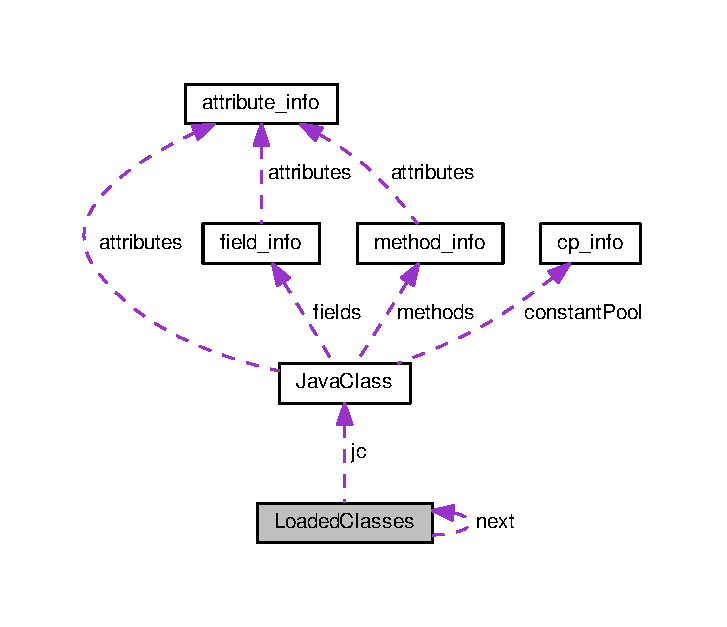
\includegraphics[width=349pt]{structLoadedClasses__coll__graph}
\end{center}
\end{figure}
\subsection*{Data Fields}
\begin{DoxyCompactItemize}
\item 
\hyperlink{structJavaClass}{Java\+Class} $\ast$ \hyperlink{structLoadedClasses_a9926f0f305ae1f117b2709b17c9084d8}{jc}
\begin{DoxyCompactList}\small\item\em Pointer to the \hyperlink{structJavaClass}{Java\+Class} struct of the resolved class. \end{DoxyCompactList}\item 
uint8\+\_\+t \hyperlink{structLoadedClasses_a4b06b6533c15ba1e1634b1e768343a84}{requires\+Init}
\begin{DoxyCompactList}\small\item\em Boolean telling if the class has already been initialized or if it still needs to be. \end{DoxyCompactList}\item 
int32\+\_\+t $\ast$ \hyperlink{structLoadedClasses_adcf48dbaaaea57b514d53a8b5a3edafe}{static\+Fields\+Data}
\begin{DoxyCompactList}\small\item\em \hyperlink{structArray}{Array} containing the data for the static fields of the class. \end{DoxyCompactList}\item 
struct \hyperlink{structLoadedClasses}{Loaded\+Classes} $\ast$ \hyperlink{structLoadedClasses_a66c15555a97e890e2967fac61bb540b8}{next}
\begin{DoxyCompactList}\small\item\em Pointer to the next node of the linked list. \end{DoxyCompactList}\end{DoxyCompactItemize}


\subsection{Detailed Description}
Linked list data struct that holds information about a class that has already been resolved. 

\subsection{Field Documentation}
\index{Loaded\+Classes@{Loaded\+Classes}!jc@{jc}}
\index{jc@{jc}!Loaded\+Classes@{Loaded\+Classes}}
\subsubsection[{\texorpdfstring{jc}{jc}}]{\setlength{\rightskip}{0pt plus 5cm}{\bf Java\+Class}$\ast$ Loaded\+Classes\+::jc}\hypertarget{structLoadedClasses_a9926f0f305ae1f117b2709b17c9084d8}{}\label{structLoadedClasses_a9926f0f305ae1f117b2709b17c9084d8}


Pointer to the \hyperlink{structJavaClass}{Java\+Class} struct of the resolved class. 

\index{Loaded\+Classes@{Loaded\+Classes}!next@{next}}
\index{next@{next}!Loaded\+Classes@{Loaded\+Classes}}
\subsubsection[{\texorpdfstring{next}{next}}]{\setlength{\rightskip}{0pt plus 5cm}struct {\bf Loaded\+Classes}$\ast$ Loaded\+Classes\+::next}\hypertarget{structLoadedClasses_a66c15555a97e890e2967fac61bb540b8}{}\label{structLoadedClasses_a66c15555a97e890e2967fac61bb540b8}


Pointer to the next node of the linked list. 

\index{Loaded\+Classes@{Loaded\+Classes}!requires\+Init@{requires\+Init}}
\index{requires\+Init@{requires\+Init}!Loaded\+Classes@{Loaded\+Classes}}
\subsubsection[{\texorpdfstring{requires\+Init}{requiresInit}}]{\setlength{\rightskip}{0pt plus 5cm}uint8\+\_\+t Loaded\+Classes\+::requires\+Init}\hypertarget{structLoadedClasses_a4b06b6533c15ba1e1634b1e768343a84}{}\label{structLoadedClasses_a4b06b6533c15ba1e1634b1e768343a84}


Boolean telling if the class has already been initialized or if it still needs to be. 

Initialization of a class is done by calling the method $<$clinit$>$ after reserving space for the static fields used by the class. Static fields with \textquotesingle{}Constant\+Value\textquotesingle{} attribute have their value set during class initialization. \begin{DoxySeeAlso}{See also}
\hyperlink{jvm_8c_ae702b2c5a05e0f39c5edcaf78bcb4c95}{init\+Class()} 
\end{DoxySeeAlso}
\index{Loaded\+Classes@{Loaded\+Classes}!static\+Fields\+Data@{static\+Fields\+Data}}
\index{static\+Fields\+Data@{static\+Fields\+Data}!Loaded\+Classes@{Loaded\+Classes}}
\subsubsection[{\texorpdfstring{static\+Fields\+Data}{staticFieldsData}}]{\setlength{\rightskip}{0pt plus 5cm}int32\+\_\+t$\ast$ Loaded\+Classes\+::static\+Fields\+Data}\hypertarget{structLoadedClasses_adcf48dbaaaea57b514d53a8b5a3edafe}{}\label{structLoadedClasses_adcf48dbaaaea57b514d53a8b5a3edafe}


\hyperlink{structArray}{Array} containing the data for the static fields of the class. 



The documentation for this struct was generated from the following file\+:\begin{DoxyCompactItemize}
\item 
src/\hyperlink{jvm_8h}{jvm.\+h}\end{DoxyCompactItemize}

\hypertarget{structmethod__info}{}\section{method\+\_\+info Struct Reference}
\label{structmethod__info}\index{method\+\_\+info@{method\+\_\+info}}


{\ttfamily \#include $<$methods.\+h$>$}



Collaboration diagram for method\+\_\+info\+:\nopagebreak
\begin{figure}[H]
\begin{center}
\leavevmode
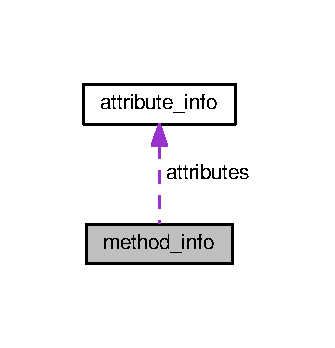
\includegraphics[width=161pt]{structmethod__info__coll__graph}
\end{center}
\end{figure}
\subsection*{Data Fields}
\begin{DoxyCompactItemize}
\item 
uint16\+\_\+t \hyperlink{structmethod__info_a8fc68aba419f2617deda879c467f5410}{access\+\_\+flags}
\item 
uint16\+\_\+t \hyperlink{structmethod__info_af0ba3d6d566432e74eed5c37cd998c14}{name\+\_\+index}
\item 
uint16\+\_\+t \hyperlink{structmethod__info_abccd6a5202d4c0ee1be6b89692d0352a}{descriptor\+\_\+index}
\item 
uint16\+\_\+t \hyperlink{structmethod__info_a9e711e4dfb8181f7dce16c6f640ba734}{attributes\+\_\+count}
\item 
\hyperlink{structattribute__info}{attribute\+\_\+info} $\ast$ \hyperlink{structmethod__info_a8ce4caaa03680c91f548558a38647ad8}{attributes}
\end{DoxyCompactItemize}


\subsection{Field Documentation}
\index{method\+\_\+info@{method\+\_\+info}!access\+\_\+flags@{access\+\_\+flags}}
\index{access\+\_\+flags@{access\+\_\+flags}!method\+\_\+info@{method\+\_\+info}}
\subsubsection[{\texorpdfstring{access\+\_\+flags}{access_flags}}]{\setlength{\rightskip}{0pt plus 5cm}uint16\+\_\+t method\+\_\+info\+::access\+\_\+flags}\hypertarget{structmethod__info_a8fc68aba419f2617deda879c467f5410}{}\label{structmethod__info_a8fc68aba419f2617deda879c467f5410}
\index{method\+\_\+info@{method\+\_\+info}!attributes@{attributes}}
\index{attributes@{attributes}!method\+\_\+info@{method\+\_\+info}}
\subsubsection[{\texorpdfstring{attributes}{attributes}}]{\setlength{\rightskip}{0pt plus 5cm}{\bf attribute\+\_\+info}$\ast$ method\+\_\+info\+::attributes}\hypertarget{structmethod__info_a8ce4caaa03680c91f548558a38647ad8}{}\label{structmethod__info_a8ce4caaa03680c91f548558a38647ad8}
\index{method\+\_\+info@{method\+\_\+info}!attributes\+\_\+count@{attributes\+\_\+count}}
\index{attributes\+\_\+count@{attributes\+\_\+count}!method\+\_\+info@{method\+\_\+info}}
\subsubsection[{\texorpdfstring{attributes\+\_\+count}{attributes_count}}]{\setlength{\rightskip}{0pt plus 5cm}uint16\+\_\+t method\+\_\+info\+::attributes\+\_\+count}\hypertarget{structmethod__info_a9e711e4dfb8181f7dce16c6f640ba734}{}\label{structmethod__info_a9e711e4dfb8181f7dce16c6f640ba734}
\index{method\+\_\+info@{method\+\_\+info}!descriptor\+\_\+index@{descriptor\+\_\+index}}
\index{descriptor\+\_\+index@{descriptor\+\_\+index}!method\+\_\+info@{method\+\_\+info}}
\subsubsection[{\texorpdfstring{descriptor\+\_\+index}{descriptor_index}}]{\setlength{\rightskip}{0pt plus 5cm}uint16\+\_\+t method\+\_\+info\+::descriptor\+\_\+index}\hypertarget{structmethod__info_abccd6a5202d4c0ee1be6b89692d0352a}{}\label{structmethod__info_abccd6a5202d4c0ee1be6b89692d0352a}
\index{method\+\_\+info@{method\+\_\+info}!name\+\_\+index@{name\+\_\+index}}
\index{name\+\_\+index@{name\+\_\+index}!method\+\_\+info@{method\+\_\+info}}
\subsubsection[{\texorpdfstring{name\+\_\+index}{name_index}}]{\setlength{\rightskip}{0pt plus 5cm}uint16\+\_\+t method\+\_\+info\+::name\+\_\+index}\hypertarget{structmethod__info_af0ba3d6d566432e74eed5c37cd998c14}{}\label{structmethod__info_af0ba3d6d566432e74eed5c37cd998c14}


The documentation for this struct was generated from the following file\+:\begin{DoxyCompactItemize}
\item 
src/\hyperlink{methods_8h}{methods.\+h}\end{DoxyCompactItemize}

\hypertarget{structObjectArray}{}\section{Object\+Array Struct Reference}
\label{structObjectArray}\index{Object\+Array@{Object\+Array}}


{\ttfamily \#include $<$jvm.\+h$>$}



Collaboration diagram for Object\+Array\+:\nopagebreak
\begin{figure}[H]
\begin{center}
\leavevmode
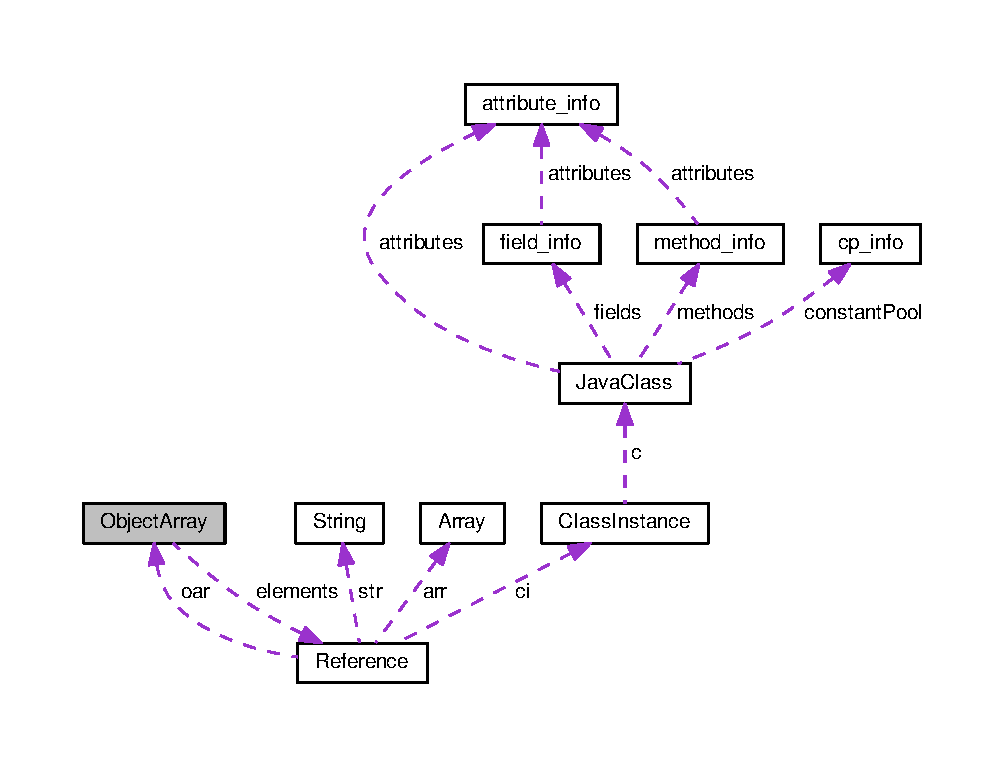
\includegraphics[width=350pt]{structObjectArray__coll__graph}
\end{center}
\end{figure}
\subsection*{Data Fields}
\begin{DoxyCompactItemize}
\item 
uint32\+\_\+t \hyperlink{structObjectArray_aa2263f92dcbf379ff869c4eefaabc715}{length}
\item 
uint8\+\_\+t $\ast$ \hyperlink{structObjectArray_a6faf7707737d9d8f5d6261334b2a5a9a}{utf8\+\_\+class\+Name}
\item 
int32\+\_\+t \hyperlink{structObjectArray_ad5fe6b2b494654afd05b58836b308d21}{utf8\+\_\+len}
\item 
\hyperlink{structReference}{Reference} $\ast$$\ast$ \hyperlink{structObjectArray_a0f945929c1656e6c0fd521bb53618f78}{elements}
\end{DoxyCompactItemize}


\subsection{Field Documentation}
\index{Object\+Array@{Object\+Array}!elements@{elements}}
\index{elements@{elements}!Object\+Array@{Object\+Array}}
\subsubsection[{\texorpdfstring{elements}{elements}}]{\setlength{\rightskip}{0pt plus 5cm}{\bf Reference}$\ast$$\ast$ Object\+Array\+::elements}\hypertarget{structObjectArray_a0f945929c1656e6c0fd521bb53618f78}{}\label{structObjectArray_a0f945929c1656e6c0fd521bb53618f78}
\index{Object\+Array@{Object\+Array}!length@{length}}
\index{length@{length}!Object\+Array@{Object\+Array}}
\subsubsection[{\texorpdfstring{length}{length}}]{\setlength{\rightskip}{0pt plus 5cm}uint32\+\_\+t Object\+Array\+::length}\hypertarget{structObjectArray_aa2263f92dcbf379ff869c4eefaabc715}{}\label{structObjectArray_aa2263f92dcbf379ff869c4eefaabc715}
\index{Object\+Array@{Object\+Array}!utf8\+\_\+class\+Name@{utf8\+\_\+class\+Name}}
\index{utf8\+\_\+class\+Name@{utf8\+\_\+class\+Name}!Object\+Array@{Object\+Array}}
\subsubsection[{\texorpdfstring{utf8\+\_\+class\+Name}{utf8_className}}]{\setlength{\rightskip}{0pt plus 5cm}uint8\+\_\+t$\ast$ Object\+Array\+::utf8\+\_\+class\+Name}\hypertarget{structObjectArray_a6faf7707737d9d8f5d6261334b2a5a9a}{}\label{structObjectArray_a6faf7707737d9d8f5d6261334b2a5a9a}
\index{Object\+Array@{Object\+Array}!utf8\+\_\+len@{utf8\+\_\+len}}
\index{utf8\+\_\+len@{utf8\+\_\+len}!Object\+Array@{Object\+Array}}
\subsubsection[{\texorpdfstring{utf8\+\_\+len}{utf8_len}}]{\setlength{\rightskip}{0pt plus 5cm}int32\+\_\+t Object\+Array\+::utf8\+\_\+len}\hypertarget{structObjectArray_ad5fe6b2b494654afd05b58836b308d21}{}\label{structObjectArray_ad5fe6b2b494654afd05b58836b308d21}


The documentation for this struct was generated from the following file\+:\begin{DoxyCompactItemize}
\item 
src/\hyperlink{jvm_8h}{jvm.\+h}\end{DoxyCompactItemize}

\hypertarget{structOperandStack}{}\section{Operand\+Stack Struct Reference}
\label{structOperandStack}\index{Operand\+Stack@{Operand\+Stack}}


{\ttfamily \#include $<$operandstack.\+h$>$}



Collaboration diagram for Operand\+Stack\+:\nopagebreak
\begin{figure}[H]
\begin{center}
\leavevmode
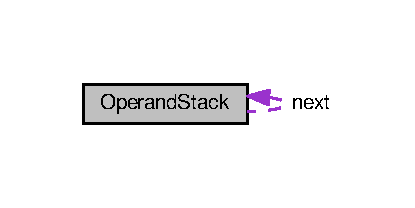
\includegraphics[width=199pt]{structOperandStack__coll__graph}
\end{center}
\end{figure}
\subsection*{Data Fields}
\begin{DoxyCompactItemize}
\item 
int32\+\_\+t \hyperlink{structOperandStack_a931d181370bfdb5b41edb8fe488c3b90}{value}
\item 
\hyperlink{operandstack_8h_aa4b9b8291a90b1a586c468110fb346a4}{Operand\+Type} \hyperlink{structOperandStack_ad7a4540e55819de1b5cebd7fd037764a}{type}
\item 
\hyperlink{structOperandStack}{Operand\+Stack} $\ast$ \hyperlink{structOperandStack_a50f11851dd7d245d2bbc7bedb0402856}{next}
\end{DoxyCompactItemize}


\subsection{Field Documentation}
\index{Operand\+Stack@{Operand\+Stack}!next@{next}}
\index{next@{next}!Operand\+Stack@{Operand\+Stack}}
\subsubsection[{\texorpdfstring{next}{next}}]{\setlength{\rightskip}{0pt plus 5cm}{\bf Operand\+Stack}$\ast$ Operand\+Stack\+::next}\hypertarget{structOperandStack_a50f11851dd7d245d2bbc7bedb0402856}{}\label{structOperandStack_a50f11851dd7d245d2bbc7bedb0402856}
\index{Operand\+Stack@{Operand\+Stack}!type@{type}}
\index{type@{type}!Operand\+Stack@{Operand\+Stack}}
\subsubsection[{\texorpdfstring{type}{type}}]{\setlength{\rightskip}{0pt plus 5cm}{\bf Operand\+Type} Operand\+Stack\+::type}\hypertarget{structOperandStack_ad7a4540e55819de1b5cebd7fd037764a}{}\label{structOperandStack_ad7a4540e55819de1b5cebd7fd037764a}
\index{Operand\+Stack@{Operand\+Stack}!value@{value}}
\index{value@{value}!Operand\+Stack@{Operand\+Stack}}
\subsubsection[{\texorpdfstring{value}{value}}]{\setlength{\rightskip}{0pt plus 5cm}int32\+\_\+t Operand\+Stack\+::value}\hypertarget{structOperandStack_a931d181370bfdb5b41edb8fe488c3b90}{}\label{structOperandStack_a931d181370bfdb5b41edb8fe488c3b90}


The documentation for this struct was generated from the following file\+:\begin{DoxyCompactItemize}
\item 
src/\hyperlink{operandstack_8h}{operandstack.\+h}\end{DoxyCompactItemize}

\hypertarget{structReference}{}\section{Reference Struct Reference}
\label{structReference}\index{Reference@{Reference}}


{\ttfamily \#include $<$jvm.\+h$>$}



Collaboration diagram for Reference\+:\nopagebreak
\begin{figure}[H]
\begin{center}
\leavevmode
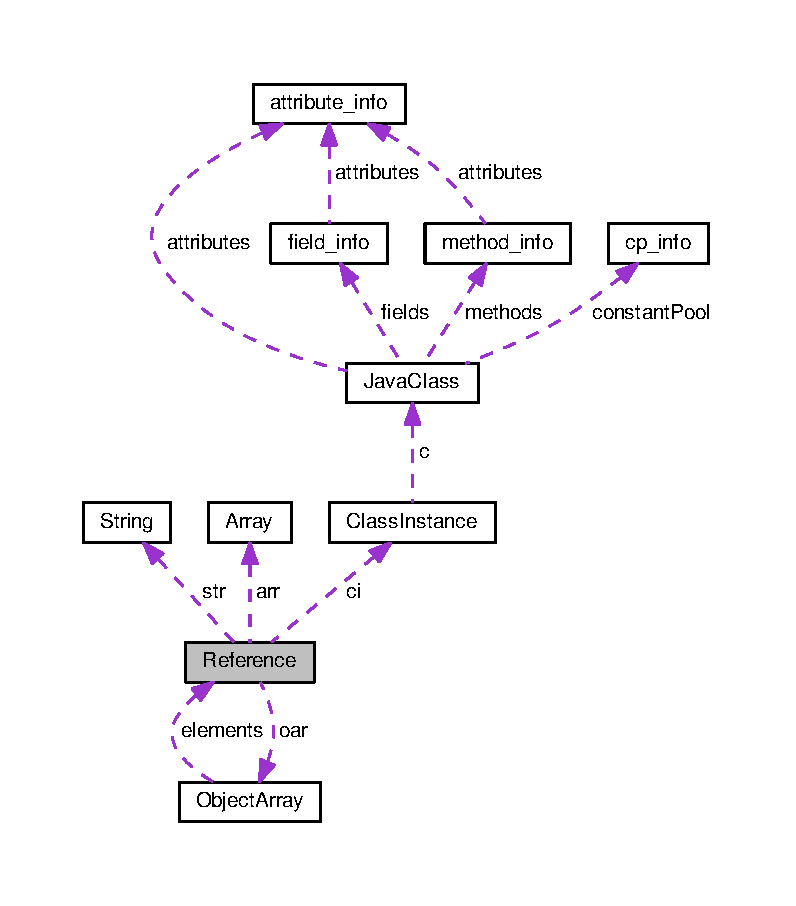
\includegraphics[width=350pt]{structReference__coll__graph}
\end{center}
\end{figure}
\subsection*{Data Fields}
\begin{DoxyCompactItemize}
\item 
\hyperlink{jvm_8h_aa298d9663bceef9c2ac2880c5bae3327}{Reference\+Type} \hyperlink{structReference_a411b420a60aa7e3ac2c0d46351dc9f13}{type}
\item 
\begin{tabbing}
xx\=xx\=xx\=xx\=xx\=xx\=xx\=xx\=xx\=\kill
union \{\\
\>\hyperlink{structClassInstance}{ClassInstance} \hyperlink{structReference_add84ffa45a635db324cfcbe73ce7074c}{ci}\\
\>\hyperlink{structArray}{Array} \hyperlink{structReference_abc67939f75b19f2e4fc35ef13ee5c407}{arr}\\
\>\hyperlink{structObjectArray}{ObjectArray} \hyperlink{structReference_a5eac3f1de74138347244ca0ef623ee24}{oar}\\
\>\hyperlink{structString}{String} \hyperlink{structReference_a64f6150b1edb24e6a4bfa5c256539d3c}{str}\\
\}; \\

\end{tabbing}\end{DoxyCompactItemize}


\subsection{Field Documentation}
\subsubsection[{\texorpdfstring{"@14}{@14}}]{\setlength{\rightskip}{0pt plus 5cm}union \{ ... \} }\hypertarget{structReference_a8b3d086534ba791fd5485da1a32205aa}{}\label{structReference_a8b3d086534ba791fd5485da1a32205aa}
\index{Reference@{Reference}!arr@{arr}}
\index{arr@{arr}!Reference@{Reference}}
\subsubsection[{\texorpdfstring{arr}{arr}}]{\setlength{\rightskip}{0pt plus 5cm}{\bf Array} Reference\+::arr}\hypertarget{structReference_abc67939f75b19f2e4fc35ef13ee5c407}{}\label{structReference_abc67939f75b19f2e4fc35ef13ee5c407}
\index{Reference@{Reference}!ci@{ci}}
\index{ci@{ci}!Reference@{Reference}}
\subsubsection[{\texorpdfstring{ci}{ci}}]{\setlength{\rightskip}{0pt plus 5cm}{\bf Class\+Instance} Reference\+::ci}\hypertarget{structReference_add84ffa45a635db324cfcbe73ce7074c}{}\label{structReference_add84ffa45a635db324cfcbe73ce7074c}
\index{Reference@{Reference}!oar@{oar}}
\index{oar@{oar}!Reference@{Reference}}
\subsubsection[{\texorpdfstring{oar}{oar}}]{\setlength{\rightskip}{0pt plus 5cm}{\bf Object\+Array} Reference\+::oar}\hypertarget{structReference_a5eac3f1de74138347244ca0ef623ee24}{}\label{structReference_a5eac3f1de74138347244ca0ef623ee24}
\index{Reference@{Reference}!str@{str}}
\index{str@{str}!Reference@{Reference}}
\subsubsection[{\texorpdfstring{str}{str}}]{\setlength{\rightskip}{0pt plus 5cm}{\bf String} Reference\+::str}\hypertarget{structReference_a64f6150b1edb24e6a4bfa5c256539d3c}{}\label{structReference_a64f6150b1edb24e6a4bfa5c256539d3c}
\index{Reference@{Reference}!type@{type}}
\index{type@{type}!Reference@{Reference}}
\subsubsection[{\texorpdfstring{type}{type}}]{\setlength{\rightskip}{0pt plus 5cm}{\bf Reference\+Type} Reference\+::type}\hypertarget{structReference_a411b420a60aa7e3ac2c0d46351dc9f13}{}\label{structReference_a411b420a60aa7e3ac2c0d46351dc9f13}


The documentation for this struct was generated from the following file\+:\begin{DoxyCompactItemize}
\item 
src/\hyperlink{jvm_8h}{jvm.\+h}\end{DoxyCompactItemize}

\hypertarget{structReferenceTable}{}\section{Reference\+Table Struct Reference}
\label{structReferenceTable}\index{Reference\+Table@{Reference\+Table}}


{\ttfamily \#include $<$jvm.\+h$>$}



Collaboration diagram for Reference\+Table\+:\nopagebreak
\begin{figure}[H]
\begin{center}
\leavevmode
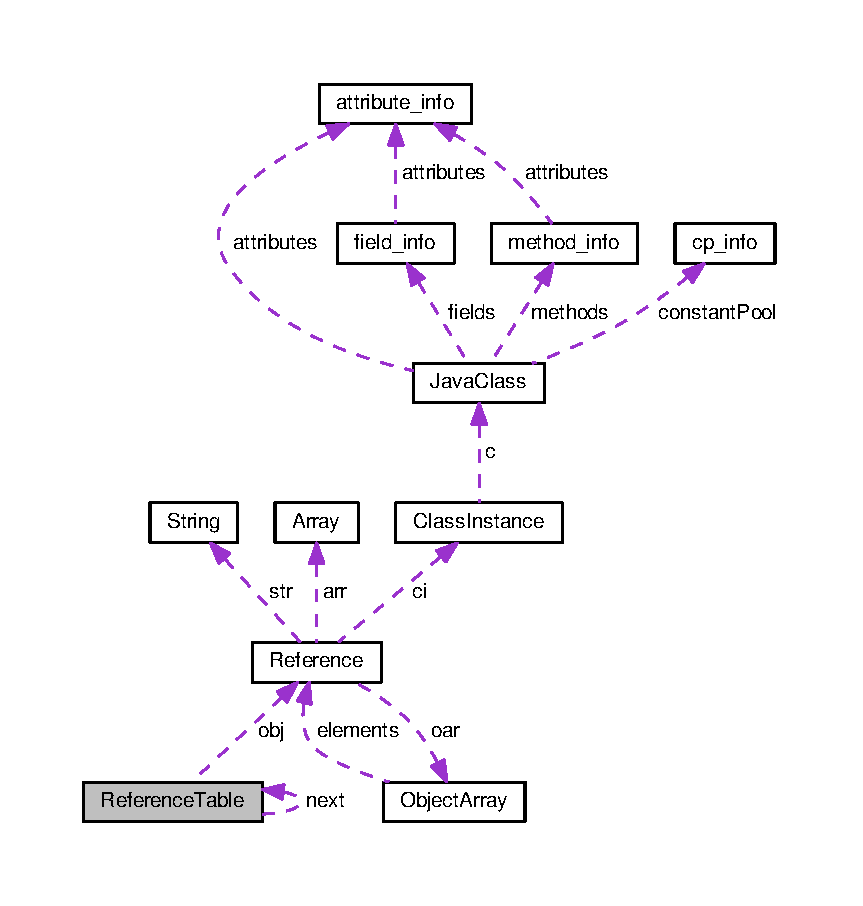
\includegraphics[width=350pt]{structReferenceTable__coll__graph}
\end{center}
\end{figure}
\subsection*{Data Fields}
\begin{DoxyCompactItemize}
\item 
\hyperlink{structReference}{Reference} $\ast$ \hyperlink{structReferenceTable_a7730da3973b57f3c86c6007b9a90e7f8}{obj}
\item 
struct \hyperlink{structReferenceTable}{Reference\+Table} $\ast$ \hyperlink{structReferenceTable_aa640983e7b43b0062fad4ca7c4b16dd4}{next}
\end{DoxyCompactItemize}


\subsection{Field Documentation}
\index{Reference\+Table@{Reference\+Table}!next@{next}}
\index{next@{next}!Reference\+Table@{Reference\+Table}}
\subsubsection[{\texorpdfstring{next}{next}}]{\setlength{\rightskip}{0pt plus 5cm}struct {\bf Reference\+Table}$\ast$ Reference\+Table\+::next}\hypertarget{structReferenceTable_aa640983e7b43b0062fad4ca7c4b16dd4}{}\label{structReferenceTable_aa640983e7b43b0062fad4ca7c4b16dd4}
\index{Reference\+Table@{Reference\+Table}!obj@{obj}}
\index{obj@{obj}!Reference\+Table@{Reference\+Table}}
\subsubsection[{\texorpdfstring{obj}{obj}}]{\setlength{\rightskip}{0pt plus 5cm}{\bf Reference}$\ast$ Reference\+Table\+::obj}\hypertarget{structReferenceTable_a7730da3973b57f3c86c6007b9a90e7f8}{}\label{structReferenceTable_a7730da3973b57f3c86c6007b9a90e7f8}


The documentation for this struct was generated from the following file\+:\begin{DoxyCompactItemize}
\item 
src/\hyperlink{jvm_8h}{jvm.\+h}\end{DoxyCompactItemize}

\hypertarget{structString}{}\section{String Struct Reference}
\label{structString}\index{String@{String}}


{\ttfamily \#include $<$jvm.\+h$>$}

\subsection*{Data Fields}
\begin{DoxyCompactItemize}
\item 
uint8\+\_\+t $\ast$ \hyperlink{structString_a9961c14ba61c6ab4b4453fd7002a09e6}{utf8\+\_\+bytes}
\item 
uint32\+\_\+t \hyperlink{structString_a83d3a7e0af08128f210cdedaecb085a2}{len}
\end{DoxyCompactItemize}


\subsection{Field Documentation}
\index{String@{String}!len@{len}}
\index{len@{len}!String@{String}}
\subsubsection[{\texorpdfstring{len}{len}}]{\setlength{\rightskip}{0pt plus 5cm}uint32\+\_\+t String\+::len}\hypertarget{structString_a83d3a7e0af08128f210cdedaecb085a2}{}\label{structString_a83d3a7e0af08128f210cdedaecb085a2}
\index{String@{String}!utf8\+\_\+bytes@{utf8\+\_\+bytes}}
\index{utf8\+\_\+bytes@{utf8\+\_\+bytes}!String@{String}}
\subsubsection[{\texorpdfstring{utf8\+\_\+bytes}{utf8_bytes}}]{\setlength{\rightskip}{0pt plus 5cm}uint8\+\_\+t$\ast$ String\+::utf8\+\_\+bytes}\hypertarget{structString_a9961c14ba61c6ab4b4453fd7002a09e6}{}\label{structString_a9961c14ba61c6ab4b4453fd7002a09e6}


The documentation for this struct was generated from the following file\+:\begin{DoxyCompactItemize}
\item 
src/\hyperlink{jvm_8h}{jvm.\+h}\end{DoxyCompactItemize}

\chapter{File Documentation}
\hypertarget{attributes_8c}{}\section{src/attributes.c File Reference}
\label{attributes_8c}\index{src/attributes.\+c@{src/attributes.\+c}}
{\ttfamily \#include \char`\"{}attributes.\+h\char`\"{}}\\*
{\ttfamily \#include \char`\"{}readfunctions.\+h\char`\"{}}\\*
{\ttfamily \#include \char`\"{}utf8.\+h\char`\"{}}\\*
{\ttfamily \#include \char`\"{}opcodes.\+h\char`\"{}}\\*
{\ttfamily \#include \char`\"{}debugging.\+h\char`\"{}}\\*
{\ttfamily \#include $<$inttypes.\+h$>$}\\*
Include dependency graph for attributes.\+c\+:\nopagebreak
\begin{figure}[H]
\begin{center}
\leavevmode
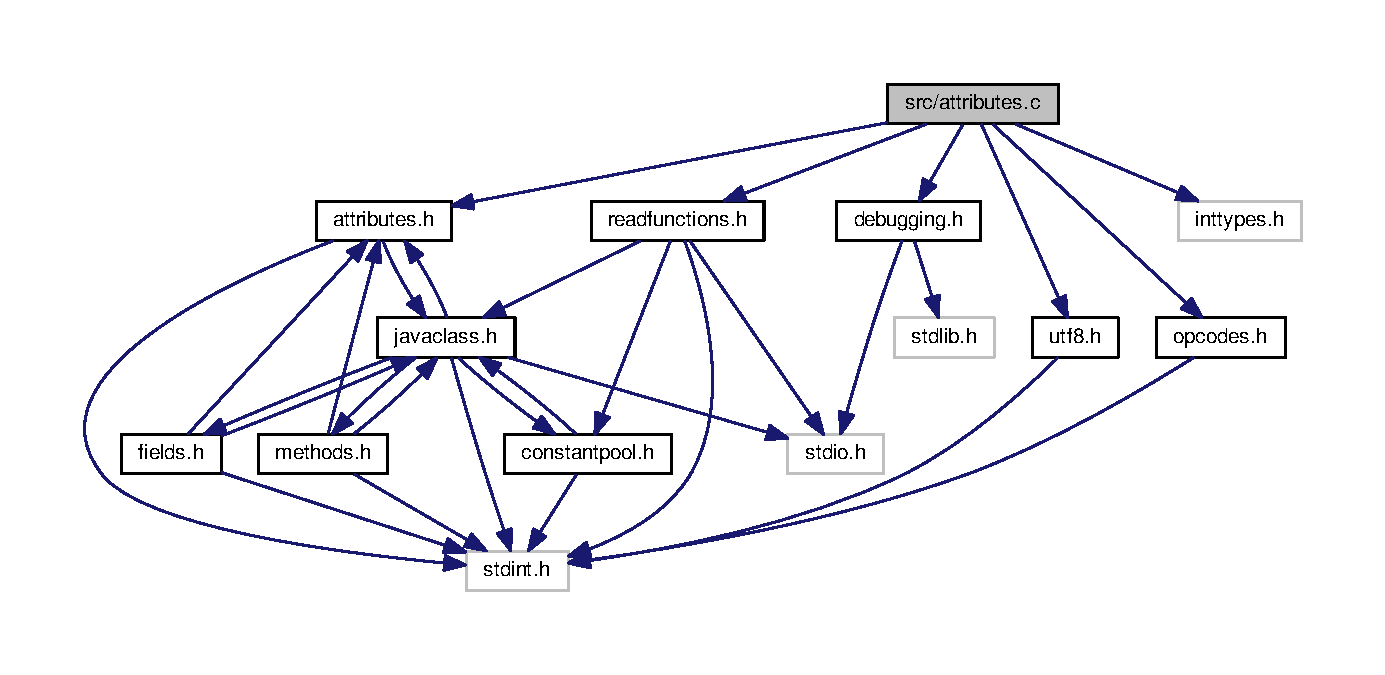
\includegraphics[width=350pt]{attributes_8c__incl}
\end{center}
\end{figure}
\subsection*{Macros}
\begin{DoxyCompactItemize}
\item 
\#define \hyperlink{attributes_8c_a1a4c6b25eeb17e81e6376d4a6383c158}{D\+E\+C\+L\+A\+R\+E\+\_\+\+A\+T\+T\+R\+\_\+\+F\+U\+N\+CS}(attr)
\item 
\#define \hyperlink{attributes_8c_afa2f48f44da881b9d32c1a7d1e4db4ab}{I\+F\+\_\+\+A\+T\+T\+R\+\_\+\+C\+H\+E\+CK}(name)
\item 
\#define \hyperlink{attributes_8c_acc32225b9d3eb1107b48de3cd4539075}{O\+P\+C\+O\+D\+E\+\_\+\+I\+N\+T\+E\+R\+V\+AL}(begin,  end)~(opcode $>$= opcode\+\_\+\#\#begin \&\& opcode $<$= opcode\+\_\+\#\#end)
\item 
\#define \hyperlink{attributes_8c_ab757e29ce18ed03f73c4b81a869e4b9a}{N\+E\+X\+T\+B\+Y\+TE}~($\ast$(info-\/$>$code + ++code\+\_\+offset))
\item 
\#define \hyperlink{attributes_8c_acd9132a8a41b59ee57e8326b1f516fa9}{A\+T\+T\+R\+\_\+\+C\+A\+SE}(attr)~case A\+T\+T\+R\+\_\+\#\#attr\+: free\+Attribute\#\#attr(entry); return;
\item 
\#define \hyperlink{attributes_8c_acd9132a8a41b59ee57e8326b1f516fa9}{A\+T\+T\+R\+\_\+\+C\+A\+SE}(attr)~case A\+T\+T\+R\+\_\+\#\#attr\+: \hyperlink{attributes_8h_aee295c33031c2ab941c9260654010db7}{print\+Attribute}\#\#attr(jc, entry, identation\+Level); break;
\end{DoxyCompactItemize}
\subsection*{Functions}
\begin{DoxyCompactItemize}
\item 
char \hyperlink{attributes_8c_a0aab7731ade76c16c2ff8b3bef1111d1}{read\+Attribute} (\hyperlink{structJavaClass}{Java\+Class} $\ast$jc, \hyperlink{structattribute__info}{attribute\+\_\+info} $\ast$entry)
\item 
void \hyperlink{attributes_8c_a01657db1f2f2e478b93e5329c666901e}{ident} (int level)
\item 
uint8\+\_\+t \hyperlink{attributes_8c_a5e568e134ff6fb82b263565076da0432}{read\+Attribute\+Deprecated} (\hyperlink{structJavaClass}{Java\+Class} $\ast$jc, \hyperlink{structattribute__info}{attribute\+\_\+info} $\ast$entry)
\item 
void \hyperlink{attributes_8c_ad80e46006ae1ca8e80f84735d331fc18}{print\+Attribute\+Deprecated} (\hyperlink{structJavaClass}{Java\+Class} $\ast$jc, \hyperlink{structattribute__info}{attribute\+\_\+info} $\ast$entry, int identation\+Level)
\item 
void \hyperlink{attributes_8c_ac122c1bdf1457e87c2cbdb8ec5ca1625}{free\+Attribute\+Deprecated} (\hyperlink{structattribute__info}{attribute\+\_\+info} $\ast$entry)
\item 
uint8\+\_\+t \hyperlink{attributes_8c_ac07fa201160b522b15c7353b4ff2ed44}{read\+Attribute\+Constant\+Value} (\hyperlink{structJavaClass}{Java\+Class} $\ast$jc, \hyperlink{structattribute__info}{attribute\+\_\+info} $\ast$entry)
\item 
void \hyperlink{attributes_8c_a5abd76089f5e6794d1ecc98cea55f158}{print\+Attribute\+Constant\+Value} (\hyperlink{structJavaClass}{Java\+Class} $\ast$jc, \hyperlink{structattribute__info}{attribute\+\_\+info} $\ast$entry, int identation\+Level)
\item 
void \hyperlink{attributes_8c_a3b65b1bc8966d4ad3a18e52ad7a3586b}{free\+Attribute\+Constant\+Value} (\hyperlink{structattribute__info}{attribute\+\_\+info} $\ast$entry)
\item 
uint8\+\_\+t \hyperlink{attributes_8c_a43bfb8cf040e623ccae73943a943a7f8}{read\+Attribute\+Source\+File} (\hyperlink{structJavaClass}{Java\+Class} $\ast$jc, \hyperlink{structattribute__info}{attribute\+\_\+info} $\ast$entry)
\item 
void \hyperlink{attributes_8c_a7566e0f5a2ba5992f6e8f84a7b5d0b8b}{print\+Attribute\+Source\+File} (\hyperlink{structJavaClass}{Java\+Class} $\ast$jc, \hyperlink{structattribute__info}{attribute\+\_\+info} $\ast$entry, int identation\+Level)
\item 
void \hyperlink{attributes_8c_ae0485d0a13108130dd232c001a4502fe}{free\+Attribute\+Source\+File} (\hyperlink{structattribute__info}{attribute\+\_\+info} $\ast$entry)
\item 
uint8\+\_\+t \hyperlink{attributes_8c_a7af979b9e909d50393f578f9cf230fae}{read\+Attribute\+Inner\+Classes} (\hyperlink{structJavaClass}{Java\+Class} $\ast$jc, \hyperlink{structattribute__info}{attribute\+\_\+info} $\ast$entry)
\item 
void \hyperlink{attributes_8c_a6c90c1dd47892d19d581ef9fcac24698}{print\+Attribute\+Inner\+Classes} (\hyperlink{structJavaClass}{Java\+Class} $\ast$jc, \hyperlink{structattribute__info}{attribute\+\_\+info} $\ast$entry, int identation\+Level)
\item 
void \hyperlink{attributes_8c_a21f76b789715d6055265e69dc63e4eeb}{free\+Attribute\+Inner\+Classes} (\hyperlink{structattribute__info}{attribute\+\_\+info} $\ast$entry)
\item 
uint8\+\_\+t \hyperlink{attributes_8c_a837af1196cf968ff688539be299648d5}{read\+Attribute\+Line\+Number\+Table} (\hyperlink{structJavaClass}{Java\+Class} $\ast$jc, \hyperlink{structattribute__info}{attribute\+\_\+info} $\ast$entry)
\item 
void \hyperlink{attributes_8c_a8c510d03555d15e558997e15e000c40f}{print\+Attribute\+Line\+Number\+Table} (\hyperlink{structJavaClass}{Java\+Class} $\ast$jc, \hyperlink{structattribute__info}{attribute\+\_\+info} $\ast$entry, int identation\+Level)
\item 
void \hyperlink{attributes_8c_af8c25d4cde9d8421cd4fefc8543d1ec7}{free\+Attribute\+Line\+Number\+Table} (\hyperlink{structattribute__info}{attribute\+\_\+info} $\ast$entry)
\item 
uint8\+\_\+t \hyperlink{attributes_8c_af3a1b04442990e1699afc5b2592c4c93}{read\+Attribute\+Code} (\hyperlink{structJavaClass}{Java\+Class} $\ast$jc, \hyperlink{structattribute__info}{attribute\+\_\+info} $\ast$entry)
\item 
void \hyperlink{attributes_8c_ae588cbde97553719c8b8612e8e42f4b4}{print\+Attribute\+Code} (\hyperlink{structJavaClass}{Java\+Class} $\ast$jc, \hyperlink{structattribute__info}{attribute\+\_\+info} $\ast$entry, int identation\+Level)
\item 
void \hyperlink{attributes_8c_a2e8c24440f4c49b6dd8a19cd9fe584c0}{free\+Attribute\+Code} (\hyperlink{structattribute__info}{attribute\+\_\+info} $\ast$entry)
\item 
uint8\+\_\+t \hyperlink{attributes_8c_a1aabfbdd22c8a11214ee3db33624b734}{read\+Attribute\+Exceptions} (\hyperlink{structJavaClass}{Java\+Class} $\ast$jc, \hyperlink{structattribute__info}{attribute\+\_\+info} $\ast$entry)
\item 
void \hyperlink{attributes_8c_a1aeef532497a7cc1a3dee89d104bd725}{print\+Attribute\+Exceptions} (\hyperlink{structJavaClass}{Java\+Class} $\ast$jc, \hyperlink{structattribute__info}{attribute\+\_\+info} $\ast$entry, int identation\+Level)
\item 
void \hyperlink{attributes_8c_a47063751996bba4e939a7d2bcebd2b10}{free\+Attribute\+Exceptions} (\hyperlink{structattribute__info}{attribute\+\_\+info} $\ast$entry)
\item 
void \hyperlink{attributes_8c_a136bdfadd787ebd62f1c721f99270cc9}{free\+Attribute\+Info} (\hyperlink{structattribute__info}{attribute\+\_\+info} $\ast$entry)
\item 
void \hyperlink{attributes_8c_aee295c33031c2ab941c9260654010db7}{print\+Attribute} (\hyperlink{structJavaClass}{Java\+Class} $\ast$jc, \hyperlink{structattribute__info}{attribute\+\_\+info} $\ast$entry, int identation\+Level)
\item 
void \hyperlink{attributes_8c_ae04e26b66957c879139f8a82e463674a}{print\+All\+Attributes} (\hyperlink{structJavaClass}{Java\+Class} $\ast$jc)
\item 
\hyperlink{structattribute__info}{attribute\+\_\+info} $\ast$ \hyperlink{attributes_8c_ae3ce1b33741046741c90a6f5592911a5}{get\+Attribute\+By\+Type} (\hyperlink{structattribute__info}{attribute\+\_\+info} $\ast$attributes, uint16\+\_\+t attributes\+\_\+length, enum \hyperlink{attributes_8h_a349a9cde14be8097df865ba0469c0ab2}{Attribute\+Type} type)
\end{DoxyCompactItemize}


\subsection{Macro Definition Documentation}
\index{attributes.\+c@{attributes.\+c}!A\+T\+T\+R\+\_\+\+C\+A\+SE@{A\+T\+T\+R\+\_\+\+C\+A\+SE}}
\index{A\+T\+T\+R\+\_\+\+C\+A\+SE@{A\+T\+T\+R\+\_\+\+C\+A\+SE}!attributes.\+c@{attributes.\+c}}
\subsubsection[{\texorpdfstring{A\+T\+T\+R\+\_\+\+C\+A\+SE}{ATTR_CASE}}]{\setlength{\rightskip}{0pt plus 5cm}\#define A\+T\+T\+R\+\_\+\+C\+A\+SE(
\begin{DoxyParamCaption}
\item[{}]{attr}
\end{DoxyParamCaption}
)~case A\+T\+T\+R\+\_\+\#\#attr\+: free\+Attribute\#\#attr(entry); return;}\hypertarget{attributes_8c_acd9132a8a41b59ee57e8326b1f516fa9}{}\label{attributes_8c_acd9132a8a41b59ee57e8326b1f516fa9}
\index{attributes.\+c@{attributes.\+c}!A\+T\+T\+R\+\_\+\+C\+A\+SE@{A\+T\+T\+R\+\_\+\+C\+A\+SE}}
\index{A\+T\+T\+R\+\_\+\+C\+A\+SE@{A\+T\+T\+R\+\_\+\+C\+A\+SE}!attributes.\+c@{attributes.\+c}}
\subsubsection[{\texorpdfstring{A\+T\+T\+R\+\_\+\+C\+A\+SE}{ATTR_CASE}}]{\setlength{\rightskip}{0pt plus 5cm}\#define A\+T\+T\+R\+\_\+\+C\+A\+SE(
\begin{DoxyParamCaption}
\item[{}]{attr}
\end{DoxyParamCaption}
)~case A\+T\+T\+R\+\_\+\#\#attr\+: {\bf print\+Attribute}\#\#attr(jc, entry, identation\+Level); break;}\hypertarget{attributes_8c_acd9132a8a41b59ee57e8326b1f516fa9}{}\label{attributes_8c_acd9132a8a41b59ee57e8326b1f516fa9}
\index{attributes.\+c@{attributes.\+c}!D\+E\+C\+L\+A\+R\+E\+\_\+\+A\+T\+T\+R\+\_\+\+F\+U\+N\+CS@{D\+E\+C\+L\+A\+R\+E\+\_\+\+A\+T\+T\+R\+\_\+\+F\+U\+N\+CS}}
\index{D\+E\+C\+L\+A\+R\+E\+\_\+\+A\+T\+T\+R\+\_\+\+F\+U\+N\+CS@{D\+E\+C\+L\+A\+R\+E\+\_\+\+A\+T\+T\+R\+\_\+\+F\+U\+N\+CS}!attributes.\+c@{attributes.\+c}}
\subsubsection[{\texorpdfstring{D\+E\+C\+L\+A\+R\+E\+\_\+\+A\+T\+T\+R\+\_\+\+F\+U\+N\+CS}{DECLARE_ATTR_FUNCS}}]{\setlength{\rightskip}{0pt plus 5cm}\#define D\+E\+C\+L\+A\+R\+E\+\_\+\+A\+T\+T\+R\+\_\+\+F\+U\+N\+CS(
\begin{DoxyParamCaption}
\item[{}]{attr}
\end{DoxyParamCaption}
)}\hypertarget{attributes_8c_a1a4c6b25eeb17e81e6376d4a6383c158}{}\label{attributes_8c_a1a4c6b25eeb17e81e6376d4a6383c158}
{\bfseries Value\+:}
\begin{DoxyCode}
uint8\_t \hyperlink{attributes_8c_a0aab7731ade76c16c2ff8b3bef1111d1}{readAttribute}##attr(\hyperlink{structJavaClass}{JavaClass}* jc, \hyperlink{structattribute__info}{attribute\_info}* entry); \(\backslash\)
    void \hyperlink{attributes_8c_aee295c33031c2ab941c9260654010db7}{printAttribute}##attr(\hyperlink{structJavaClass}{JavaClass}* jc, 
      \hyperlink{structattribute__info}{attribute\_info}* entry, \textcolor{keywordtype}{int} identationLevel); \(\backslash\)
    void freeAttribute##attr(\hyperlink{structattribute__info}{attribute\_info}* entry);
\end{DoxyCode}
\index{attributes.\+c@{attributes.\+c}!I\+F\+\_\+\+A\+T\+T\+R\+\_\+\+C\+H\+E\+CK@{I\+F\+\_\+\+A\+T\+T\+R\+\_\+\+C\+H\+E\+CK}}
\index{I\+F\+\_\+\+A\+T\+T\+R\+\_\+\+C\+H\+E\+CK@{I\+F\+\_\+\+A\+T\+T\+R\+\_\+\+C\+H\+E\+CK}!attributes.\+c@{attributes.\+c}}
\subsubsection[{\texorpdfstring{I\+F\+\_\+\+A\+T\+T\+R\+\_\+\+C\+H\+E\+CK}{IF_ATTR_CHECK}}]{\setlength{\rightskip}{0pt plus 5cm}\#define I\+F\+\_\+\+A\+T\+T\+R\+\_\+\+C\+H\+E\+CK(
\begin{DoxyParamCaption}
\item[{}]{name}
\end{DoxyParamCaption}
)}\hypertarget{attributes_8c_afa2f48f44da881b9d32c1a7d1e4db4ab}{}\label{attributes_8c_afa2f48f44da881b9d32c1a7d1e4db4ab}
{\bfseries Value\+:}
\begin{DoxyCode}
\textcolor{keywordflow}{if} (\hyperlink{utf8_8c_a317c1d4f6b0e4b61b5f99baf9d673a8e}{cmp\_UTF8\_Ascii}(cp->Utf8.bytes, cp->Utf8.length, (uint8\_t*)#name, \textcolor{keyword}{sizeof}(#name) - 1)) \{ \(\backslash\)
            entry->attributeType = ATTR\_##name; \(\backslash\)
            result = \hyperlink{attributes_8c_a0aab7731ade76c16c2ff8b3bef1111d1}{readAttribute}##name(jc, entry); \(\backslash\)
        \}
\end{DoxyCode}
\index{attributes.\+c@{attributes.\+c}!N\+E\+X\+T\+B\+Y\+TE@{N\+E\+X\+T\+B\+Y\+TE}}
\index{N\+E\+X\+T\+B\+Y\+TE@{N\+E\+X\+T\+B\+Y\+TE}!attributes.\+c@{attributes.\+c}}
\subsubsection[{\texorpdfstring{N\+E\+X\+T\+B\+Y\+TE}{NEXTBYTE}}]{\setlength{\rightskip}{0pt plus 5cm}\#define N\+E\+X\+T\+B\+Y\+TE~($\ast$(info-\/$>$code + ++code\+\_\+offset))}\hypertarget{attributes_8c_ab757e29ce18ed03f73c4b81a869e4b9a}{}\label{attributes_8c_ab757e29ce18ed03f73c4b81a869e4b9a}
\index{attributes.\+c@{attributes.\+c}!O\+P\+C\+O\+D\+E\+\_\+\+I\+N\+T\+E\+R\+V\+AL@{O\+P\+C\+O\+D\+E\+\_\+\+I\+N\+T\+E\+R\+V\+AL}}
\index{O\+P\+C\+O\+D\+E\+\_\+\+I\+N\+T\+E\+R\+V\+AL@{O\+P\+C\+O\+D\+E\+\_\+\+I\+N\+T\+E\+R\+V\+AL}!attributes.\+c@{attributes.\+c}}
\subsubsection[{\texorpdfstring{O\+P\+C\+O\+D\+E\+\_\+\+I\+N\+T\+E\+R\+V\+AL}{OPCODE_INTERVAL}}]{\setlength{\rightskip}{0pt plus 5cm}\#define O\+P\+C\+O\+D\+E\+\_\+\+I\+N\+T\+E\+R\+V\+AL(
\begin{DoxyParamCaption}
\item[{}]{begin, }
\item[{}]{end}
\end{DoxyParamCaption}
)~(opcode $>$= opcode\+\_\+\#\#begin \&\& opcode $<$= opcode\+\_\+\#\#end)}\hypertarget{attributes_8c_acc32225b9d3eb1107b48de3cd4539075}{}\label{attributes_8c_acc32225b9d3eb1107b48de3cd4539075}


\subsection{Function Documentation}
\index{attributes.\+c@{attributes.\+c}!free\+Attribute\+Code@{free\+Attribute\+Code}}
\index{free\+Attribute\+Code@{free\+Attribute\+Code}!attributes.\+c@{attributes.\+c}}
\subsubsection[{\texorpdfstring{free\+Attribute\+Code(attribute\+\_\+info $\ast$entry)}{freeAttributeCode(attribute_info *entry)}}]{\setlength{\rightskip}{0pt plus 5cm}void free\+Attribute\+Code (
\begin{DoxyParamCaption}
\item[{{\bf attribute\+\_\+info} $\ast$}]{entry}
\end{DoxyParamCaption}
)}\hypertarget{attributes_8c_a2e8c24440f4c49b6dd8a19cd9fe584c0}{}\label{attributes_8c_a2e8c24440f4c49b6dd8a19cd9fe584c0}


Here is the call graph for this function\+:\nopagebreak
\begin{figure}[H]
\begin{center}
\leavevmode
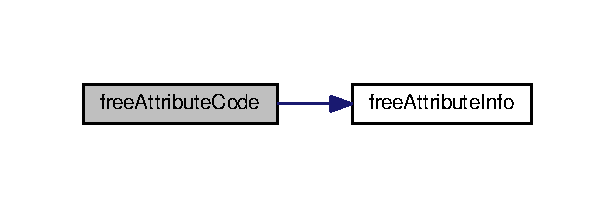
\includegraphics[width=295pt]{attributes_8c_a2e8c24440f4c49b6dd8a19cd9fe584c0_cgraph}
\end{center}
\end{figure}


\index{attributes.\+c@{attributes.\+c}!free\+Attribute\+Constant\+Value@{free\+Attribute\+Constant\+Value}}
\index{free\+Attribute\+Constant\+Value@{free\+Attribute\+Constant\+Value}!attributes.\+c@{attributes.\+c}}
\subsubsection[{\texorpdfstring{free\+Attribute\+Constant\+Value(attribute\+\_\+info $\ast$entry)}{freeAttributeConstantValue(attribute_info *entry)}}]{\setlength{\rightskip}{0pt plus 5cm}void free\+Attribute\+Constant\+Value (
\begin{DoxyParamCaption}
\item[{{\bf attribute\+\_\+info} $\ast$}]{entry}
\end{DoxyParamCaption}
)}\hypertarget{attributes_8c_a3b65b1bc8966d4ad3a18e52ad7a3586b}{}\label{attributes_8c_a3b65b1bc8966d4ad3a18e52ad7a3586b}
\index{attributes.\+c@{attributes.\+c}!free\+Attribute\+Deprecated@{free\+Attribute\+Deprecated}}
\index{free\+Attribute\+Deprecated@{free\+Attribute\+Deprecated}!attributes.\+c@{attributes.\+c}}
\subsubsection[{\texorpdfstring{free\+Attribute\+Deprecated(attribute\+\_\+info $\ast$entry)}{freeAttributeDeprecated(attribute_info *entry)}}]{\setlength{\rightskip}{0pt plus 5cm}void free\+Attribute\+Deprecated (
\begin{DoxyParamCaption}
\item[{{\bf attribute\+\_\+info} $\ast$}]{entry}
\end{DoxyParamCaption}
)}\hypertarget{attributes_8c_ac122c1bdf1457e87c2cbdb8ec5ca1625}{}\label{attributes_8c_ac122c1bdf1457e87c2cbdb8ec5ca1625}
\index{attributes.\+c@{attributes.\+c}!free\+Attribute\+Exceptions@{free\+Attribute\+Exceptions}}
\index{free\+Attribute\+Exceptions@{free\+Attribute\+Exceptions}!attributes.\+c@{attributes.\+c}}
\subsubsection[{\texorpdfstring{free\+Attribute\+Exceptions(attribute\+\_\+info $\ast$entry)}{freeAttributeExceptions(attribute_info *entry)}}]{\setlength{\rightskip}{0pt plus 5cm}void free\+Attribute\+Exceptions (
\begin{DoxyParamCaption}
\item[{{\bf attribute\+\_\+info} $\ast$}]{entry}
\end{DoxyParamCaption}
)}\hypertarget{attributes_8c_a47063751996bba4e939a7d2bcebd2b10}{}\label{attributes_8c_a47063751996bba4e939a7d2bcebd2b10}
\index{attributes.\+c@{attributes.\+c}!free\+Attribute\+Info@{free\+Attribute\+Info}}
\index{free\+Attribute\+Info@{free\+Attribute\+Info}!attributes.\+c@{attributes.\+c}}
\subsubsection[{\texorpdfstring{free\+Attribute\+Info(attribute\+\_\+info $\ast$entry)}{freeAttributeInfo(attribute_info *entry)}}]{\setlength{\rightskip}{0pt plus 5cm}void free\+Attribute\+Info (
\begin{DoxyParamCaption}
\item[{{\bf attribute\+\_\+info} $\ast$}]{entry}
\end{DoxyParamCaption}
)}\hypertarget{attributes_8c_a136bdfadd787ebd62f1c721f99270cc9}{}\label{attributes_8c_a136bdfadd787ebd62f1c721f99270cc9}


Here is the caller graph for this function\+:\nopagebreak
\begin{figure}[H]
\begin{center}
\leavevmode
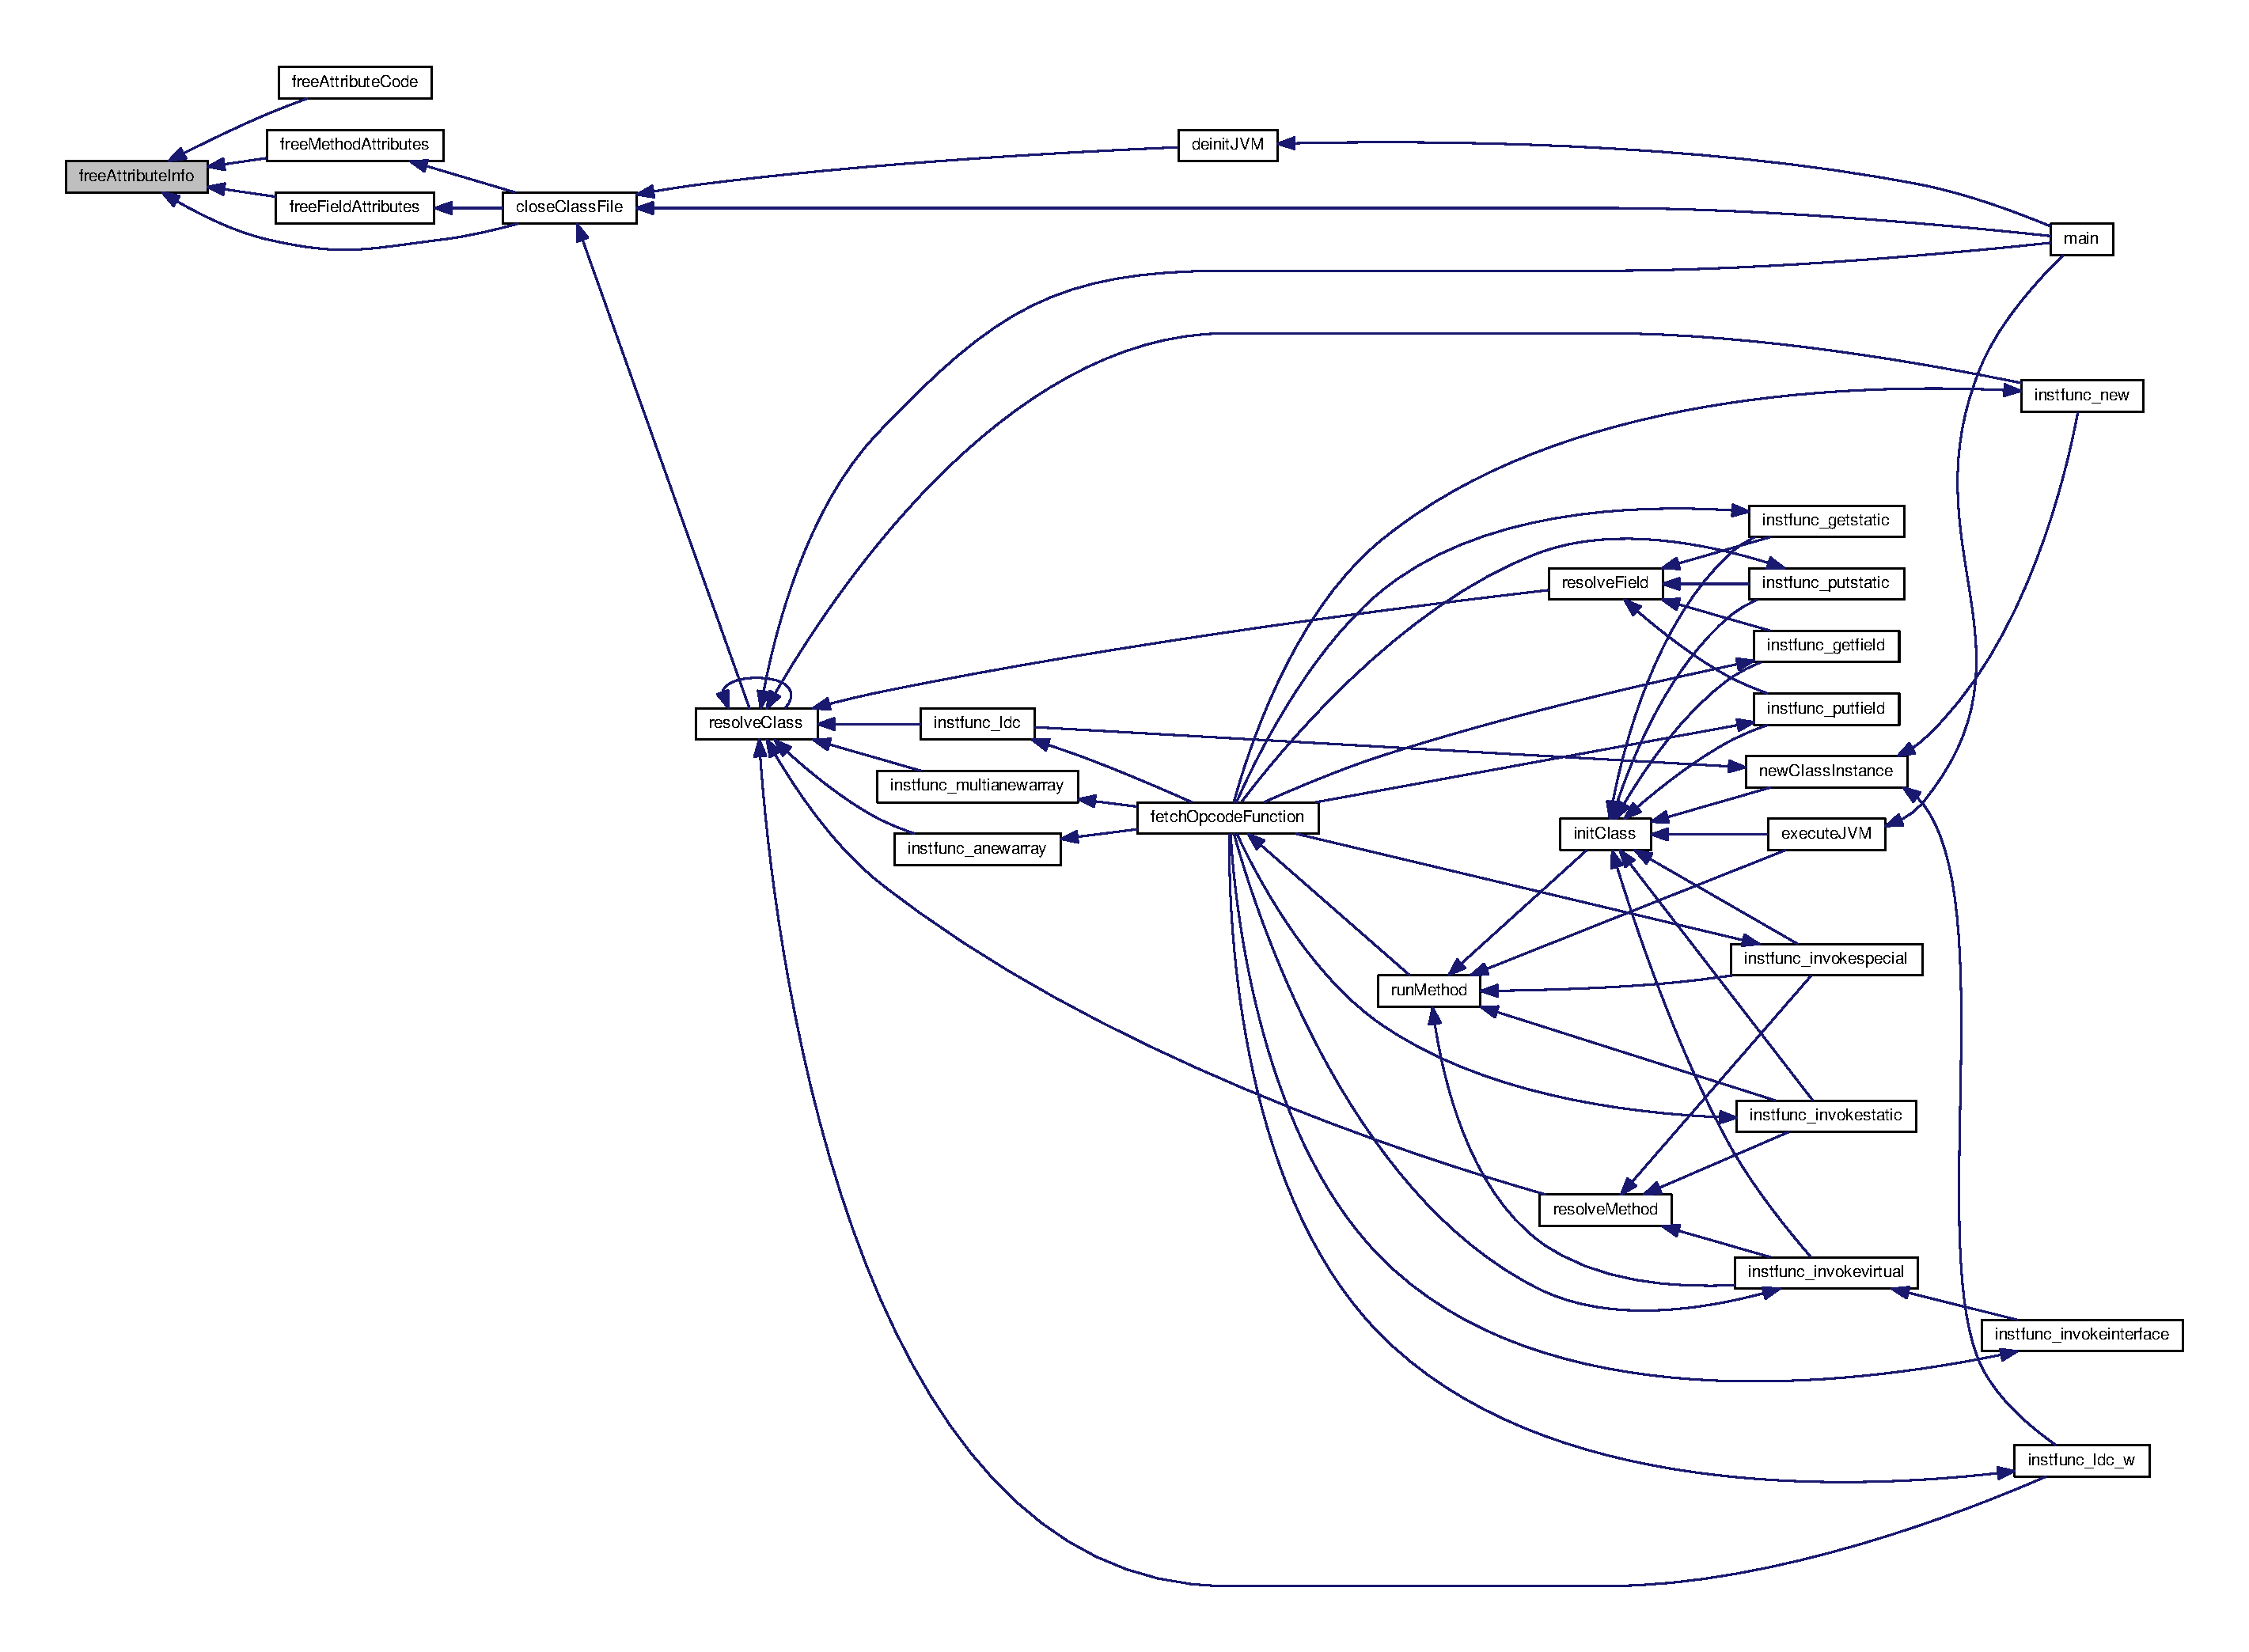
\includegraphics[width=350pt]{attributes_8c_a136bdfadd787ebd62f1c721f99270cc9_icgraph}
\end{center}
\end{figure}


\index{attributes.\+c@{attributes.\+c}!free\+Attribute\+Inner\+Classes@{free\+Attribute\+Inner\+Classes}}
\index{free\+Attribute\+Inner\+Classes@{free\+Attribute\+Inner\+Classes}!attributes.\+c@{attributes.\+c}}
\subsubsection[{\texorpdfstring{free\+Attribute\+Inner\+Classes(attribute\+\_\+info $\ast$entry)}{freeAttributeInnerClasses(attribute_info *entry)}}]{\setlength{\rightskip}{0pt plus 5cm}void free\+Attribute\+Inner\+Classes (
\begin{DoxyParamCaption}
\item[{{\bf attribute\+\_\+info} $\ast$}]{entry}
\end{DoxyParamCaption}
)}\hypertarget{attributes_8c_a21f76b789715d6055265e69dc63e4eeb}{}\label{attributes_8c_a21f76b789715d6055265e69dc63e4eeb}
\index{attributes.\+c@{attributes.\+c}!free\+Attribute\+Line\+Number\+Table@{free\+Attribute\+Line\+Number\+Table}}
\index{free\+Attribute\+Line\+Number\+Table@{free\+Attribute\+Line\+Number\+Table}!attributes.\+c@{attributes.\+c}}
\subsubsection[{\texorpdfstring{free\+Attribute\+Line\+Number\+Table(attribute\+\_\+info $\ast$entry)}{freeAttributeLineNumberTable(attribute_info *entry)}}]{\setlength{\rightskip}{0pt plus 5cm}void free\+Attribute\+Line\+Number\+Table (
\begin{DoxyParamCaption}
\item[{{\bf attribute\+\_\+info} $\ast$}]{entry}
\end{DoxyParamCaption}
)}\hypertarget{attributes_8c_af8c25d4cde9d8421cd4fefc8543d1ec7}{}\label{attributes_8c_af8c25d4cde9d8421cd4fefc8543d1ec7}
\index{attributes.\+c@{attributes.\+c}!free\+Attribute\+Source\+File@{free\+Attribute\+Source\+File}}
\index{free\+Attribute\+Source\+File@{free\+Attribute\+Source\+File}!attributes.\+c@{attributes.\+c}}
\subsubsection[{\texorpdfstring{free\+Attribute\+Source\+File(attribute\+\_\+info $\ast$entry)}{freeAttributeSourceFile(attribute_info *entry)}}]{\setlength{\rightskip}{0pt plus 5cm}void free\+Attribute\+Source\+File (
\begin{DoxyParamCaption}
\item[{{\bf attribute\+\_\+info} $\ast$}]{entry}
\end{DoxyParamCaption}
)}\hypertarget{attributes_8c_ae0485d0a13108130dd232c001a4502fe}{}\label{attributes_8c_ae0485d0a13108130dd232c001a4502fe}
\index{attributes.\+c@{attributes.\+c}!get\+Attribute\+By\+Type@{get\+Attribute\+By\+Type}}
\index{get\+Attribute\+By\+Type@{get\+Attribute\+By\+Type}!attributes.\+c@{attributes.\+c}}
\subsubsection[{\texorpdfstring{get\+Attribute\+By\+Type(attribute\+\_\+info $\ast$attributes, uint16\+\_\+t attributes\+\_\+length, enum Attribute\+Type type)}{getAttributeByType(attribute_info *attributes, uint16_t attributes_length, enum AttributeType type)}}]{\setlength{\rightskip}{0pt plus 5cm}{\bf attribute\+\_\+info}$\ast$ get\+Attribute\+By\+Type (
\begin{DoxyParamCaption}
\item[{{\bf attribute\+\_\+info} $\ast$}]{attributes, }
\item[{uint16\+\_\+t}]{attributes\+\_\+length, }
\item[{enum {\bf Attribute\+Type}}]{type}
\end{DoxyParamCaption}
)}\hypertarget{attributes_8c_ae3ce1b33741046741c90a6f5592911a5}{}\label{attributes_8c_ae3ce1b33741046741c90a6f5592911a5}


Here is the caller graph for this function\+:\nopagebreak
\begin{figure}[H]
\begin{center}
\leavevmode
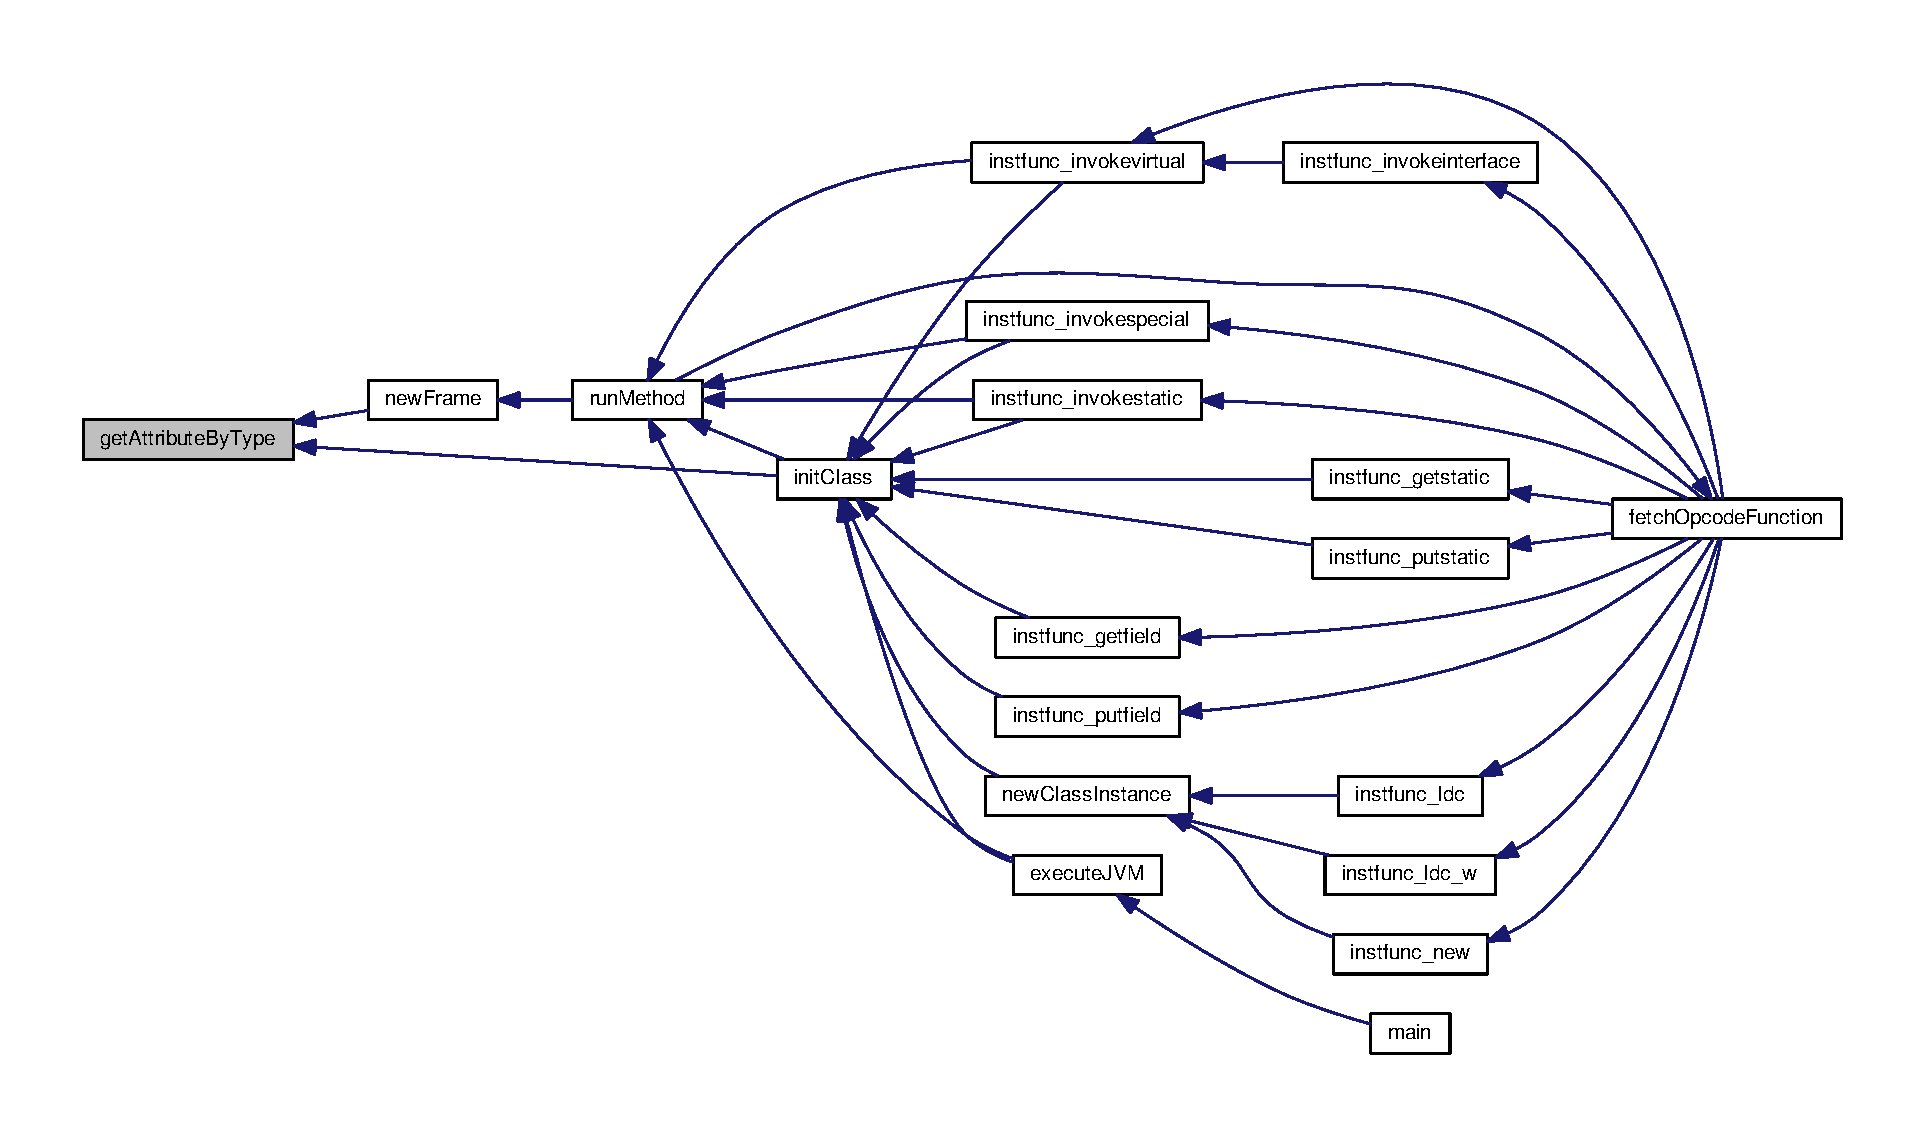
\includegraphics[width=350pt]{attributes_8c_ae3ce1b33741046741c90a6f5592911a5_icgraph}
\end{center}
\end{figure}


\index{attributes.\+c@{attributes.\+c}!ident@{ident}}
\index{ident@{ident}!attributes.\+c@{attributes.\+c}}
\subsubsection[{\texorpdfstring{ident(int level)}{ident(int level)}}]{\setlength{\rightskip}{0pt plus 5cm}void ident (
\begin{DoxyParamCaption}
\item[{int}]{level}
\end{DoxyParamCaption}
)}\hypertarget{attributes_8c_a01657db1f2f2e478b93e5329c666901e}{}\label{attributes_8c_a01657db1f2f2e478b93e5329c666901e}


Here is the caller graph for this function\+:\nopagebreak
\begin{figure}[H]
\begin{center}
\leavevmode
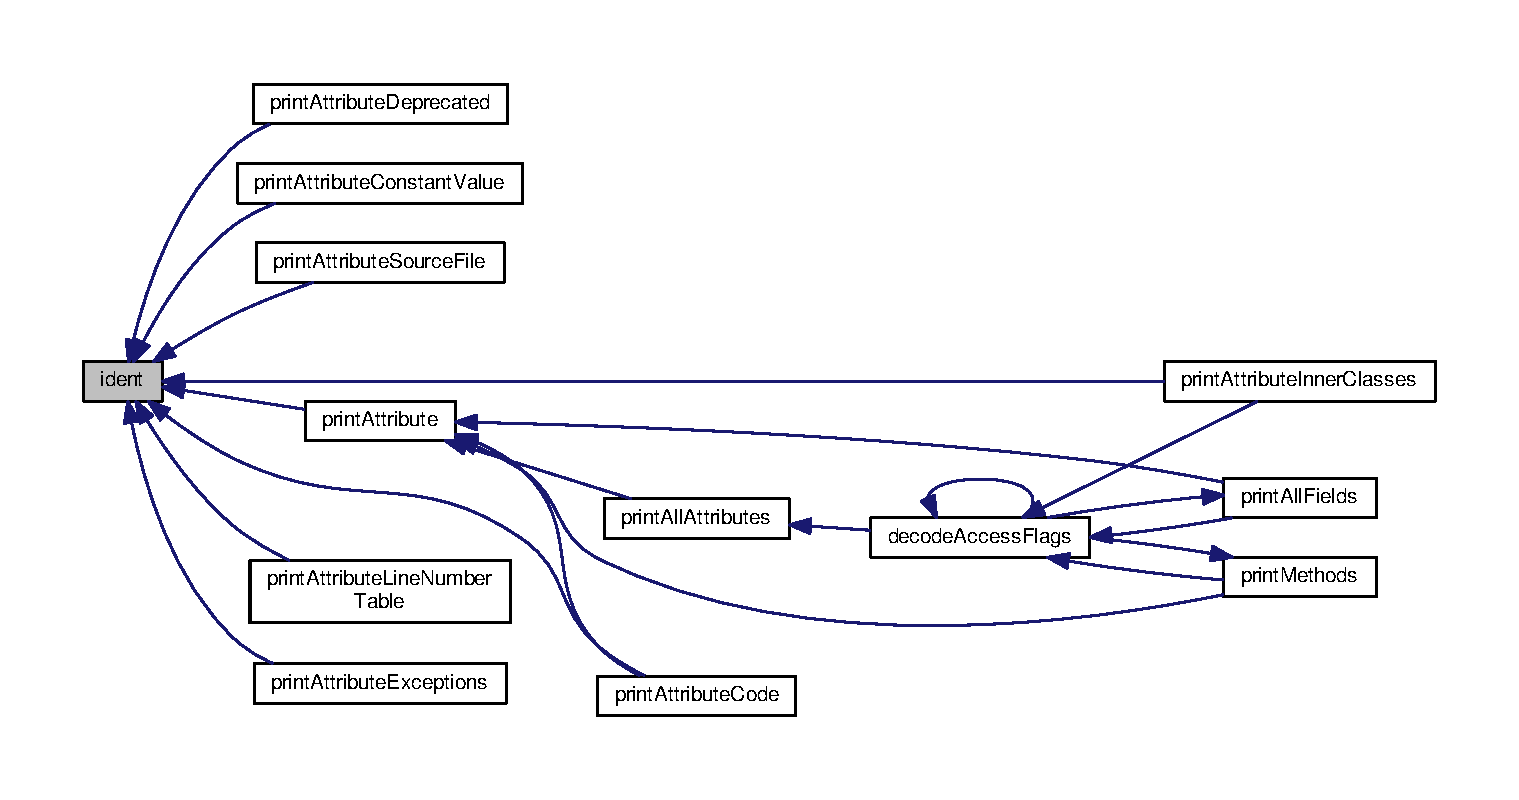
\includegraphics[width=350pt]{attributes_8c_a01657db1f2f2e478b93e5329c666901e_icgraph}
\end{center}
\end{figure}


\index{attributes.\+c@{attributes.\+c}!print\+All\+Attributes@{print\+All\+Attributes}}
\index{print\+All\+Attributes@{print\+All\+Attributes}!attributes.\+c@{attributes.\+c}}
\subsubsection[{\texorpdfstring{print\+All\+Attributes(\+Java\+Class $\ast$jc)}{printAllAttributes(JavaClass *jc)}}]{\setlength{\rightskip}{0pt plus 5cm}void print\+All\+Attributes (
\begin{DoxyParamCaption}
\item[{{\bf Java\+Class} $\ast$}]{jc}
\end{DoxyParamCaption}
)}\hypertarget{attributes_8c_ae04e26b66957c879139f8a82e463674a}{}\label{attributes_8c_ae04e26b66957c879139f8a82e463674a}


Here is the call graph for this function\+:\nopagebreak
\begin{figure}[H]
\begin{center}
\leavevmode
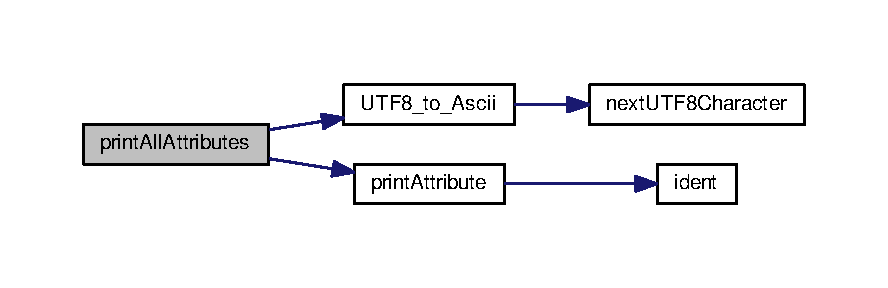
\includegraphics[width=350pt]{attributes_8c_ae04e26b66957c879139f8a82e463674a_cgraph}
\end{center}
\end{figure}




Here is the caller graph for this function\+:\nopagebreak
\begin{figure}[H]
\begin{center}
\leavevmode
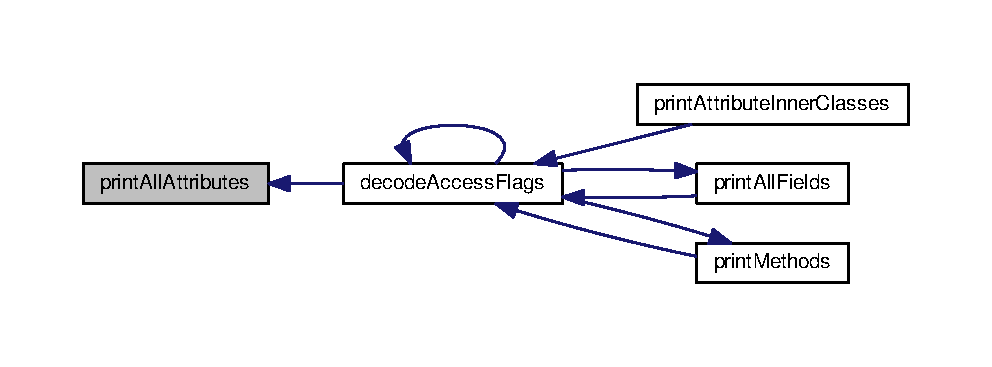
\includegraphics[width=350pt]{attributes_8c_ae04e26b66957c879139f8a82e463674a_icgraph}
\end{center}
\end{figure}


\index{attributes.\+c@{attributes.\+c}!print\+Attribute@{print\+Attribute}}
\index{print\+Attribute@{print\+Attribute}!attributes.\+c@{attributes.\+c}}
\subsubsection[{\texorpdfstring{print\+Attribute(\+Java\+Class $\ast$jc, attribute\+\_\+info $\ast$entry, int identation\+Level)}{printAttribute(JavaClass *jc, attribute_info *entry, int identationLevel)}}]{\setlength{\rightskip}{0pt plus 5cm}void print\+Attribute (
\begin{DoxyParamCaption}
\item[{{\bf Java\+Class} $\ast$}]{jc, }
\item[{{\bf attribute\+\_\+info} $\ast$}]{entry, }
\item[{int}]{identation\+Level}
\end{DoxyParamCaption}
)}\hypertarget{attributes_8c_aee295c33031c2ab941c9260654010db7}{}\label{attributes_8c_aee295c33031c2ab941c9260654010db7}


Here is the call graph for this function\+:\nopagebreak
\begin{figure}[H]
\begin{center}
\leavevmode
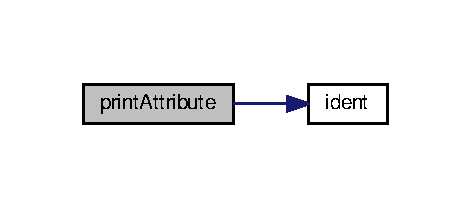
\includegraphics[width=226pt]{attributes_8c_aee295c33031c2ab941c9260654010db7_cgraph}
\end{center}
\end{figure}




Here is the caller graph for this function\+:\nopagebreak
\begin{figure}[H]
\begin{center}
\leavevmode
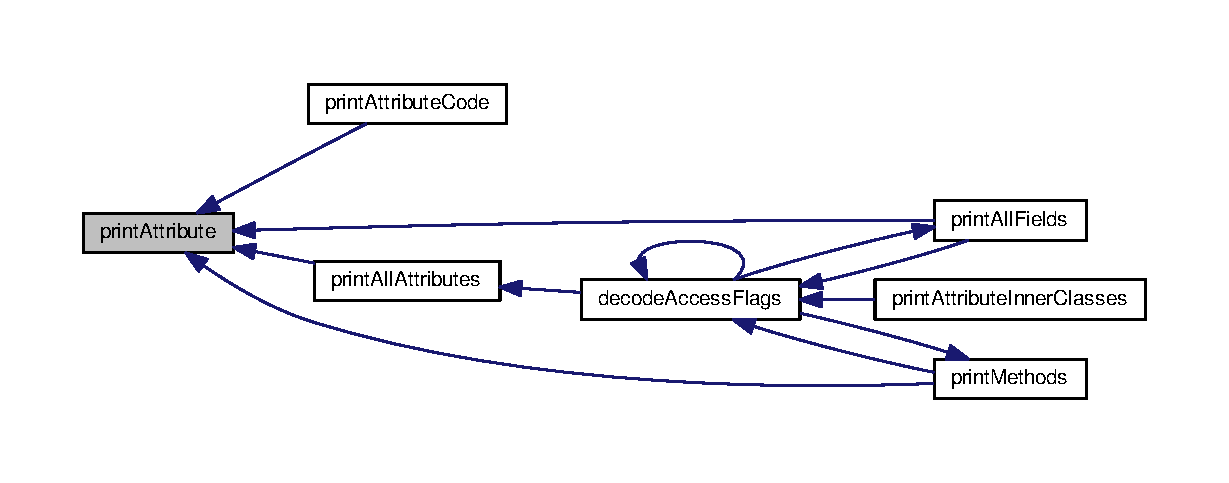
\includegraphics[width=350pt]{attributes_8c_aee295c33031c2ab941c9260654010db7_icgraph}
\end{center}
\end{figure}


\index{attributes.\+c@{attributes.\+c}!print\+Attribute\+Code@{print\+Attribute\+Code}}
\index{print\+Attribute\+Code@{print\+Attribute\+Code}!attributes.\+c@{attributes.\+c}}
\subsubsection[{\texorpdfstring{print\+Attribute\+Code(\+Java\+Class $\ast$jc, attribute\+\_\+info $\ast$entry, int identation\+Level)}{printAttributeCode(JavaClass *jc, attribute_info *entry, int identationLevel)}}]{\setlength{\rightskip}{0pt plus 5cm}void print\+Attribute\+Code (
\begin{DoxyParamCaption}
\item[{{\bf Java\+Class} $\ast$}]{jc, }
\item[{{\bf attribute\+\_\+info} $\ast$}]{entry, }
\item[{int}]{identation\+Level}
\end{DoxyParamCaption}
)}\hypertarget{attributes_8c_ae588cbde97553719c8b8612e8e42f4b4}{}\label{attributes_8c_ae588cbde97553719c8b8612e8e42f4b4}


Here is the call graph for this function\+:\nopagebreak
\begin{figure}[H]
\begin{center}
\leavevmode
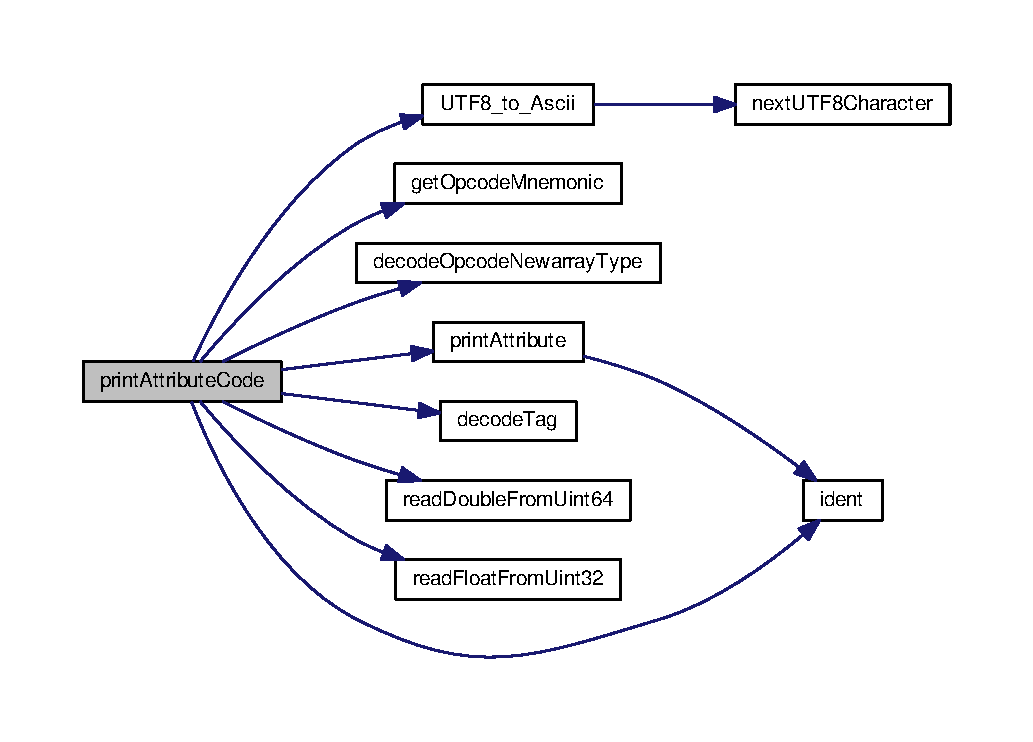
\includegraphics[width=350pt]{attributes_8c_ae588cbde97553719c8b8612e8e42f4b4_cgraph}
\end{center}
\end{figure}


\index{attributes.\+c@{attributes.\+c}!print\+Attribute\+Constant\+Value@{print\+Attribute\+Constant\+Value}}
\index{print\+Attribute\+Constant\+Value@{print\+Attribute\+Constant\+Value}!attributes.\+c@{attributes.\+c}}
\subsubsection[{\texorpdfstring{print\+Attribute\+Constant\+Value(\+Java\+Class $\ast$jc, attribute\+\_\+info $\ast$entry, int identation\+Level)}{printAttributeConstantValue(JavaClass *jc, attribute_info *entry, int identationLevel)}}]{\setlength{\rightskip}{0pt plus 5cm}void print\+Attribute\+Constant\+Value (
\begin{DoxyParamCaption}
\item[{{\bf Java\+Class} $\ast$}]{jc, }
\item[{{\bf attribute\+\_\+info} $\ast$}]{entry, }
\item[{int}]{identation\+Level}
\end{DoxyParamCaption}
)}\hypertarget{attributes_8c_a5abd76089f5e6794d1ecc98cea55f158}{}\label{attributes_8c_a5abd76089f5e6794d1ecc98cea55f158}


Here is the call graph for this function\+:\nopagebreak
\begin{figure}[H]
\begin{center}
\leavevmode
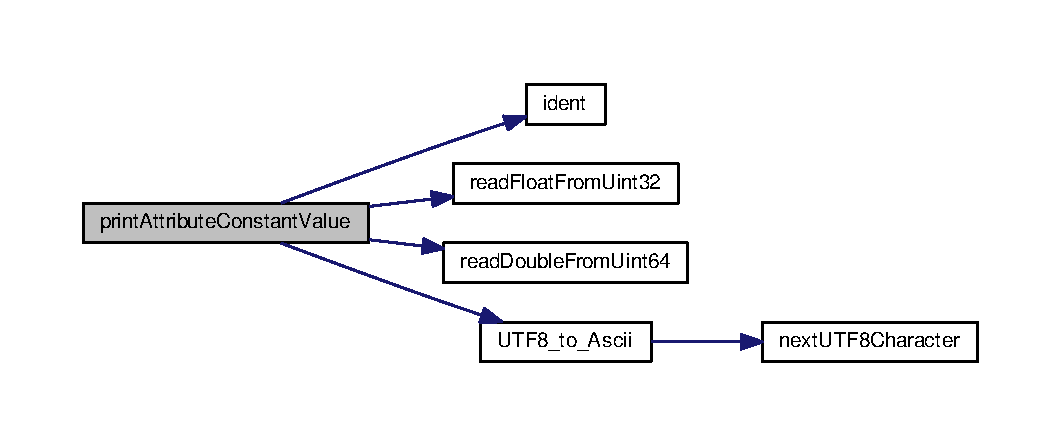
\includegraphics[width=350pt]{attributes_8c_a5abd76089f5e6794d1ecc98cea55f158_cgraph}
\end{center}
\end{figure}


\index{attributes.\+c@{attributes.\+c}!print\+Attribute\+Deprecated@{print\+Attribute\+Deprecated}}
\index{print\+Attribute\+Deprecated@{print\+Attribute\+Deprecated}!attributes.\+c@{attributes.\+c}}
\subsubsection[{\texorpdfstring{print\+Attribute\+Deprecated(\+Java\+Class $\ast$jc, attribute\+\_\+info $\ast$entry, int identation\+Level)}{printAttributeDeprecated(JavaClass *jc, attribute_info *entry, int identationLevel)}}]{\setlength{\rightskip}{0pt plus 5cm}void print\+Attribute\+Deprecated (
\begin{DoxyParamCaption}
\item[{{\bf Java\+Class} $\ast$}]{jc, }
\item[{{\bf attribute\+\_\+info} $\ast$}]{entry, }
\item[{int}]{identation\+Level}
\end{DoxyParamCaption}
)}\hypertarget{attributes_8c_ad80e46006ae1ca8e80f84735d331fc18}{}\label{attributes_8c_ad80e46006ae1ca8e80f84735d331fc18}


Here is the call graph for this function\+:\nopagebreak
\begin{figure}[H]
\begin{center}
\leavevmode
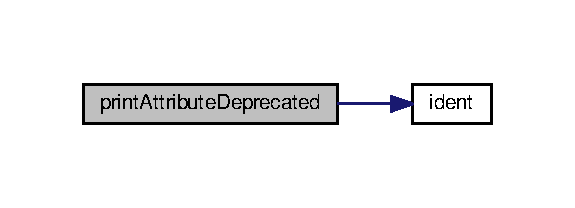
\includegraphics[width=276pt]{attributes_8c_ad80e46006ae1ca8e80f84735d331fc18_cgraph}
\end{center}
\end{figure}


\index{attributes.\+c@{attributes.\+c}!print\+Attribute\+Exceptions@{print\+Attribute\+Exceptions}}
\index{print\+Attribute\+Exceptions@{print\+Attribute\+Exceptions}!attributes.\+c@{attributes.\+c}}
\subsubsection[{\texorpdfstring{print\+Attribute\+Exceptions(\+Java\+Class $\ast$jc, attribute\+\_\+info $\ast$entry, int identation\+Level)}{printAttributeExceptions(JavaClass *jc, attribute_info *entry, int identationLevel)}}]{\setlength{\rightskip}{0pt plus 5cm}void print\+Attribute\+Exceptions (
\begin{DoxyParamCaption}
\item[{{\bf Java\+Class} $\ast$}]{jc, }
\item[{{\bf attribute\+\_\+info} $\ast$}]{entry, }
\item[{int}]{identation\+Level}
\end{DoxyParamCaption}
)}\hypertarget{attributes_8c_a1aeef532497a7cc1a3dee89d104bd725}{}\label{attributes_8c_a1aeef532497a7cc1a3dee89d104bd725}


Here is the call graph for this function\+:\nopagebreak
\begin{figure}[H]
\begin{center}
\leavevmode
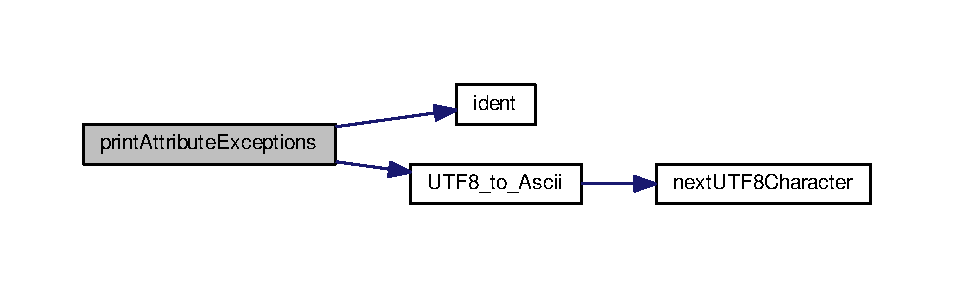
\includegraphics[width=350pt]{attributes_8c_a1aeef532497a7cc1a3dee89d104bd725_cgraph}
\end{center}
\end{figure}


\index{attributes.\+c@{attributes.\+c}!print\+Attribute\+Inner\+Classes@{print\+Attribute\+Inner\+Classes}}
\index{print\+Attribute\+Inner\+Classes@{print\+Attribute\+Inner\+Classes}!attributes.\+c@{attributes.\+c}}
\subsubsection[{\texorpdfstring{print\+Attribute\+Inner\+Classes(\+Java\+Class $\ast$jc, attribute\+\_\+info $\ast$entry, int identation\+Level)}{printAttributeInnerClasses(JavaClass *jc, attribute_info *entry, int identationLevel)}}]{\setlength{\rightskip}{0pt plus 5cm}void print\+Attribute\+Inner\+Classes (
\begin{DoxyParamCaption}
\item[{{\bf Java\+Class} $\ast$}]{jc, }
\item[{{\bf attribute\+\_\+info} $\ast$}]{entry, }
\item[{int}]{identation\+Level}
\end{DoxyParamCaption}
)}\hypertarget{attributes_8c_a6c90c1dd47892d19d581ef9fcac24698}{}\label{attributes_8c_a6c90c1dd47892d19d581ef9fcac24698}


Here is the call graph for this function\+:\nopagebreak
\begin{figure}[H]
\begin{center}
\leavevmode
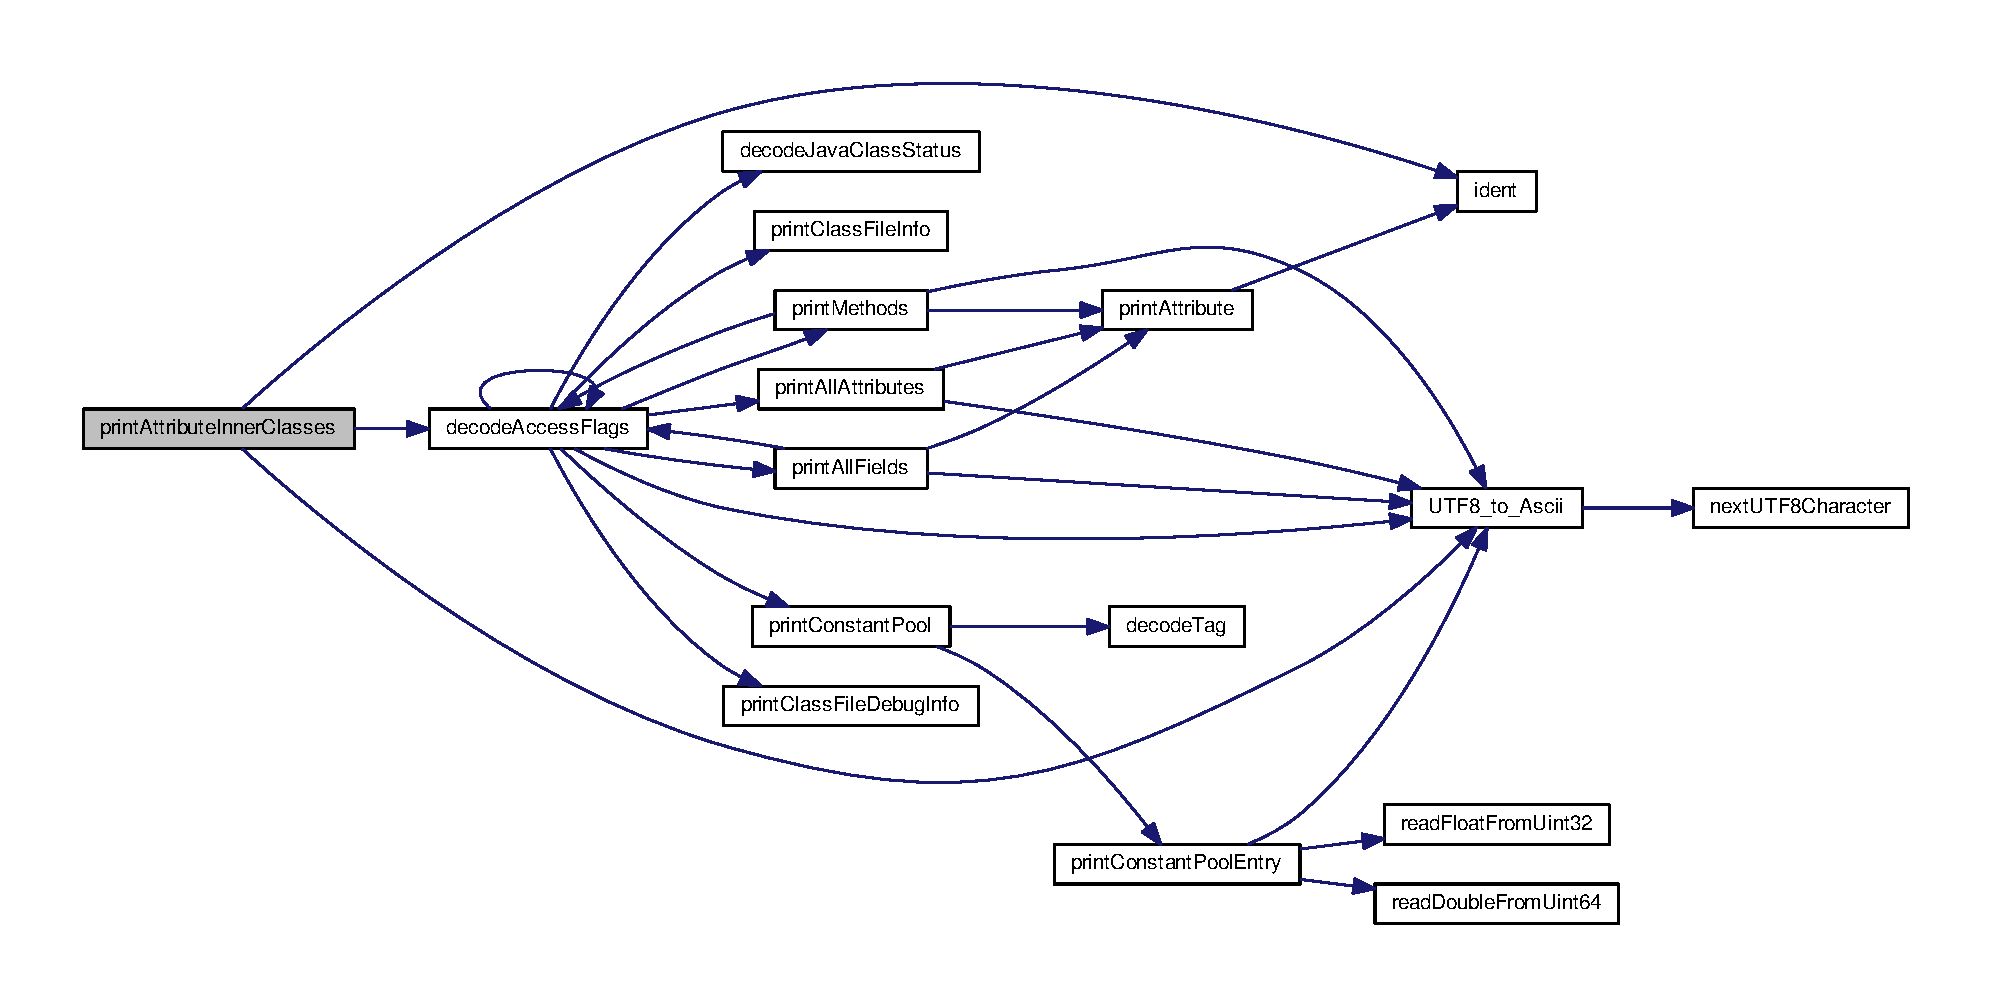
\includegraphics[width=350pt]{attributes_8c_a6c90c1dd47892d19d581ef9fcac24698_cgraph}
\end{center}
\end{figure}


\index{attributes.\+c@{attributes.\+c}!print\+Attribute\+Line\+Number\+Table@{print\+Attribute\+Line\+Number\+Table}}
\index{print\+Attribute\+Line\+Number\+Table@{print\+Attribute\+Line\+Number\+Table}!attributes.\+c@{attributes.\+c}}
\subsubsection[{\texorpdfstring{print\+Attribute\+Line\+Number\+Table(\+Java\+Class $\ast$jc, attribute\+\_\+info $\ast$entry, int identation\+Level)}{printAttributeLineNumberTable(JavaClass *jc, attribute_info *entry, int identationLevel)}}]{\setlength{\rightskip}{0pt plus 5cm}void print\+Attribute\+Line\+Number\+Table (
\begin{DoxyParamCaption}
\item[{{\bf Java\+Class} $\ast$}]{jc, }
\item[{{\bf attribute\+\_\+info} $\ast$}]{entry, }
\item[{int}]{identation\+Level}
\end{DoxyParamCaption}
)}\hypertarget{attributes_8c_a8c510d03555d15e558997e15e000c40f}{}\label{attributes_8c_a8c510d03555d15e558997e15e000c40f}


Here is the call graph for this function\+:\nopagebreak
\begin{figure}[H]
\begin{center}
\leavevmode
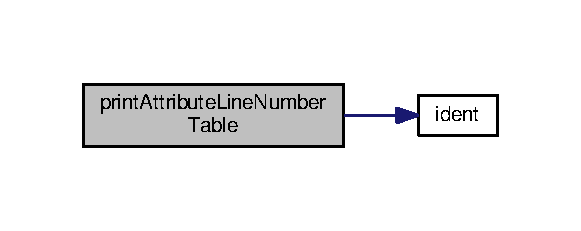
\includegraphics[width=279pt]{attributes_8c_a8c510d03555d15e558997e15e000c40f_cgraph}
\end{center}
\end{figure}


\index{attributes.\+c@{attributes.\+c}!print\+Attribute\+Source\+File@{print\+Attribute\+Source\+File}}
\index{print\+Attribute\+Source\+File@{print\+Attribute\+Source\+File}!attributes.\+c@{attributes.\+c}}
\subsubsection[{\texorpdfstring{print\+Attribute\+Source\+File(\+Java\+Class $\ast$jc, attribute\+\_\+info $\ast$entry, int identation\+Level)}{printAttributeSourceFile(JavaClass *jc, attribute_info *entry, int identationLevel)}}]{\setlength{\rightskip}{0pt plus 5cm}void print\+Attribute\+Source\+File (
\begin{DoxyParamCaption}
\item[{{\bf Java\+Class} $\ast$}]{jc, }
\item[{{\bf attribute\+\_\+info} $\ast$}]{entry, }
\item[{int}]{identation\+Level}
\end{DoxyParamCaption}
)}\hypertarget{attributes_8c_a7566e0f5a2ba5992f6e8f84a7b5d0b8b}{}\label{attributes_8c_a7566e0f5a2ba5992f6e8f84a7b5d0b8b}


Here is the call graph for this function\+:\nopagebreak
\begin{figure}[H]
\begin{center}
\leavevmode
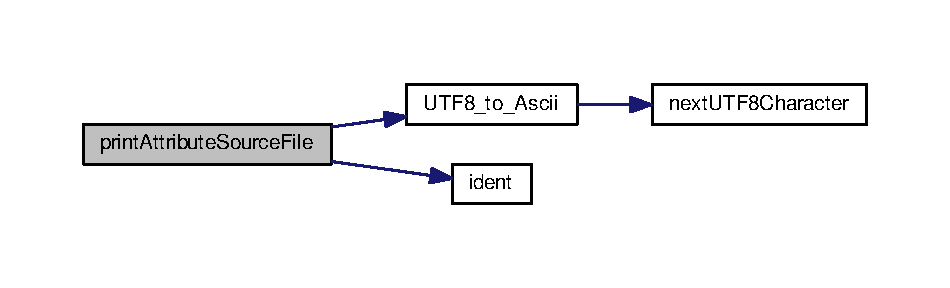
\includegraphics[width=350pt]{attributes_8c_a7566e0f5a2ba5992f6e8f84a7b5d0b8b_cgraph}
\end{center}
\end{figure}


\index{attributes.\+c@{attributes.\+c}!read\+Attribute@{read\+Attribute}}
\index{read\+Attribute@{read\+Attribute}!attributes.\+c@{attributes.\+c}}
\subsubsection[{\texorpdfstring{read\+Attribute(\+Java\+Class $\ast$jc, attribute\+\_\+info $\ast$entry)}{readAttribute(JavaClass *jc, attribute_info *entry)}}]{\setlength{\rightskip}{0pt plus 5cm}char read\+Attribute (
\begin{DoxyParamCaption}
\item[{{\bf Java\+Class} $\ast$}]{jc, }
\item[{{\bf attribute\+\_\+info} $\ast$}]{entry}
\end{DoxyParamCaption}
)}\hypertarget{attributes_8c_a0aab7731ade76c16c2ff8b3bef1111d1}{}\label{attributes_8c_a0aab7731ade76c16c2ff8b3bef1111d1}


Here is the call graph for this function\+:\nopagebreak
\begin{figure}[H]
\begin{center}
\leavevmode
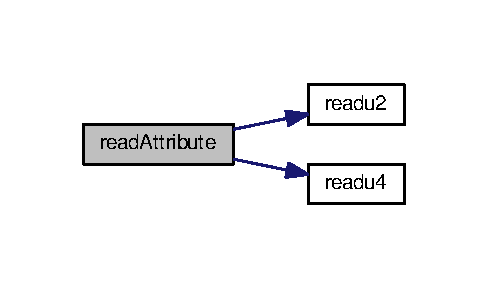
\includegraphics[width=234pt]{attributes_8c_a0aab7731ade76c16c2ff8b3bef1111d1_cgraph}
\end{center}
\end{figure}




Here is the caller graph for this function\+:\nopagebreak
\begin{figure}[H]
\begin{center}
\leavevmode
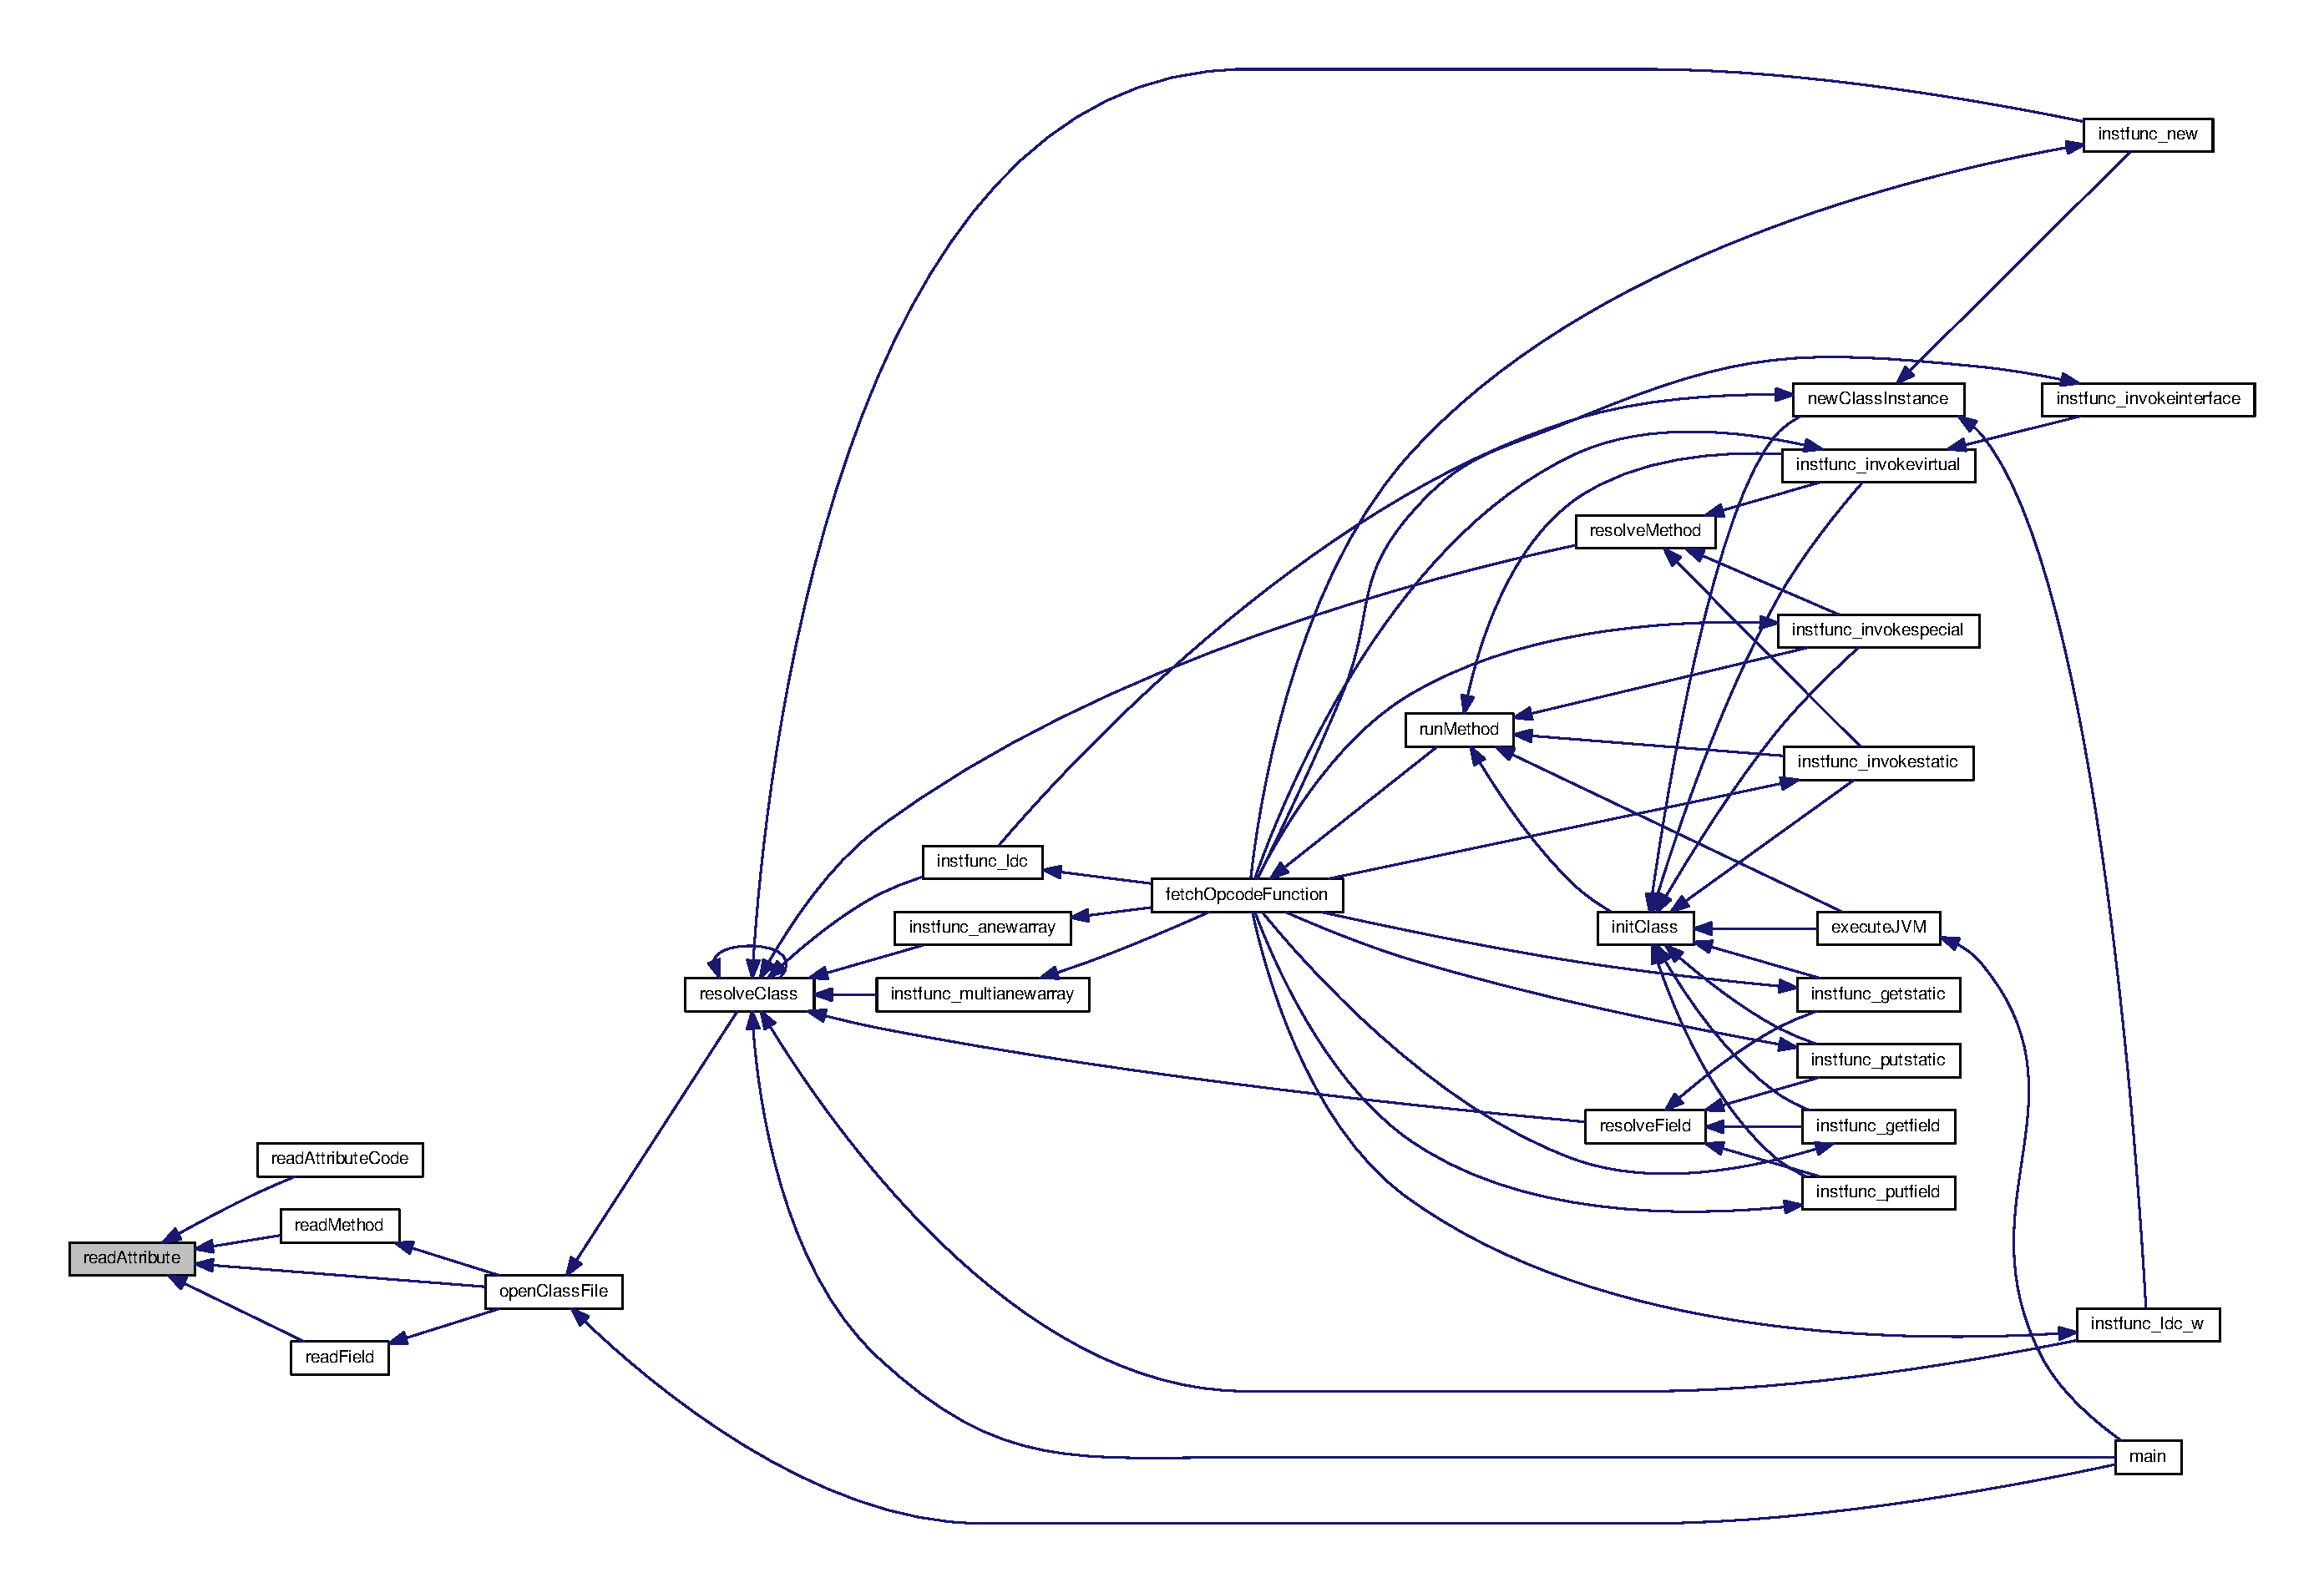
\includegraphics[width=350pt]{attributes_8c_a0aab7731ade76c16c2ff8b3bef1111d1_icgraph}
\end{center}
\end{figure}


\index{attributes.\+c@{attributes.\+c}!read\+Attribute\+Code@{read\+Attribute\+Code}}
\index{read\+Attribute\+Code@{read\+Attribute\+Code}!attributes.\+c@{attributes.\+c}}
\subsubsection[{\texorpdfstring{read\+Attribute\+Code(\+Java\+Class $\ast$jc, attribute\+\_\+info $\ast$entry)}{readAttributeCode(JavaClass *jc, attribute_info *entry)}}]{\setlength{\rightskip}{0pt plus 5cm}uint8\+\_\+t read\+Attribute\+Code (
\begin{DoxyParamCaption}
\item[{{\bf Java\+Class} $\ast$}]{jc, }
\item[{{\bf attribute\+\_\+info} $\ast$}]{entry}
\end{DoxyParamCaption}
)}\hypertarget{attributes_8c_af3a1b04442990e1699afc5b2592c4c93}{}\label{attributes_8c_af3a1b04442990e1699afc5b2592c4c93}


Here is the call graph for this function\+:\nopagebreak
\begin{figure}[H]
\begin{center}
\leavevmode
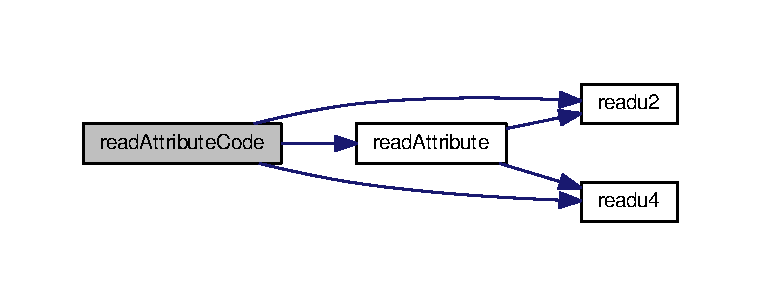
\includegraphics[width=350pt]{attributes_8c_af3a1b04442990e1699afc5b2592c4c93_cgraph}
\end{center}
\end{figure}


\index{attributes.\+c@{attributes.\+c}!read\+Attribute\+Constant\+Value@{read\+Attribute\+Constant\+Value}}
\index{read\+Attribute\+Constant\+Value@{read\+Attribute\+Constant\+Value}!attributes.\+c@{attributes.\+c}}
\subsubsection[{\texorpdfstring{read\+Attribute\+Constant\+Value(\+Java\+Class $\ast$jc, attribute\+\_\+info $\ast$entry)}{readAttributeConstantValue(JavaClass *jc, attribute_info *entry)}}]{\setlength{\rightskip}{0pt plus 5cm}uint8\+\_\+t read\+Attribute\+Constant\+Value (
\begin{DoxyParamCaption}
\item[{{\bf Java\+Class} $\ast$}]{jc, }
\item[{{\bf attribute\+\_\+info} $\ast$}]{entry}
\end{DoxyParamCaption}
)}\hypertarget{attributes_8c_ac07fa201160b522b15c7353b4ff2ed44}{}\label{attributes_8c_ac07fa201160b522b15c7353b4ff2ed44}


Here is the call graph for this function\+:\nopagebreak
\begin{figure}[H]
\begin{center}
\leavevmode
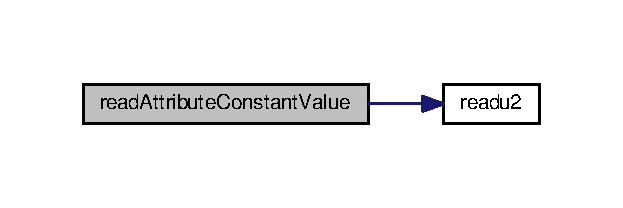
\includegraphics[width=299pt]{attributes_8c_ac07fa201160b522b15c7353b4ff2ed44_cgraph}
\end{center}
\end{figure}


\index{attributes.\+c@{attributes.\+c}!read\+Attribute\+Deprecated@{read\+Attribute\+Deprecated}}
\index{read\+Attribute\+Deprecated@{read\+Attribute\+Deprecated}!attributes.\+c@{attributes.\+c}}
\subsubsection[{\texorpdfstring{read\+Attribute\+Deprecated(\+Java\+Class $\ast$jc, attribute\+\_\+info $\ast$entry)}{readAttributeDeprecated(JavaClass *jc, attribute_info *entry)}}]{\setlength{\rightskip}{0pt plus 5cm}uint8\+\_\+t read\+Attribute\+Deprecated (
\begin{DoxyParamCaption}
\item[{{\bf Java\+Class} $\ast$}]{jc, }
\item[{{\bf attribute\+\_\+info} $\ast$}]{entry}
\end{DoxyParamCaption}
)}\hypertarget{attributes_8c_a5e568e134ff6fb82b263565076da0432}{}\label{attributes_8c_a5e568e134ff6fb82b263565076da0432}
\index{attributes.\+c@{attributes.\+c}!read\+Attribute\+Exceptions@{read\+Attribute\+Exceptions}}
\index{read\+Attribute\+Exceptions@{read\+Attribute\+Exceptions}!attributes.\+c@{attributes.\+c}}
\subsubsection[{\texorpdfstring{read\+Attribute\+Exceptions(\+Java\+Class $\ast$jc, attribute\+\_\+info $\ast$entry)}{readAttributeExceptions(JavaClass *jc, attribute_info *entry)}}]{\setlength{\rightskip}{0pt plus 5cm}uint8\+\_\+t read\+Attribute\+Exceptions (
\begin{DoxyParamCaption}
\item[{{\bf Java\+Class} $\ast$}]{jc, }
\item[{{\bf attribute\+\_\+info} $\ast$}]{entry}
\end{DoxyParamCaption}
)}\hypertarget{attributes_8c_a1aabfbdd22c8a11214ee3db33624b734}{}\label{attributes_8c_a1aabfbdd22c8a11214ee3db33624b734}


Here is the call graph for this function\+:\nopagebreak
\begin{figure}[H]
\begin{center}
\leavevmode
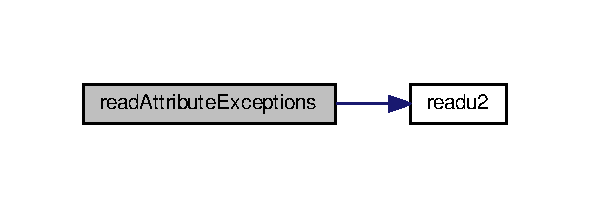
\includegraphics[width=283pt]{attributes_8c_a1aabfbdd22c8a11214ee3db33624b734_cgraph}
\end{center}
\end{figure}


\index{attributes.\+c@{attributes.\+c}!read\+Attribute\+Inner\+Classes@{read\+Attribute\+Inner\+Classes}}
\index{read\+Attribute\+Inner\+Classes@{read\+Attribute\+Inner\+Classes}!attributes.\+c@{attributes.\+c}}
\subsubsection[{\texorpdfstring{read\+Attribute\+Inner\+Classes(\+Java\+Class $\ast$jc, attribute\+\_\+info $\ast$entry)}{readAttributeInnerClasses(JavaClass *jc, attribute_info *entry)}}]{\setlength{\rightskip}{0pt plus 5cm}uint8\+\_\+t read\+Attribute\+Inner\+Classes (
\begin{DoxyParamCaption}
\item[{{\bf Java\+Class} $\ast$}]{jc, }
\item[{{\bf attribute\+\_\+info} $\ast$}]{entry}
\end{DoxyParamCaption}
)}\hypertarget{attributes_8c_a7af979b9e909d50393f578f9cf230fae}{}\label{attributes_8c_a7af979b9e909d50393f578f9cf230fae}


Here is the call graph for this function\+:\nopagebreak
\begin{figure}[H]
\begin{center}
\leavevmode
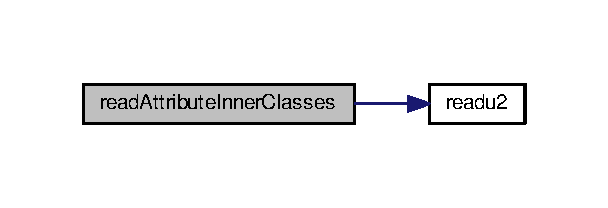
\includegraphics[width=292pt]{attributes_8c_a7af979b9e909d50393f578f9cf230fae_cgraph}
\end{center}
\end{figure}


\index{attributes.\+c@{attributes.\+c}!read\+Attribute\+Line\+Number\+Table@{read\+Attribute\+Line\+Number\+Table}}
\index{read\+Attribute\+Line\+Number\+Table@{read\+Attribute\+Line\+Number\+Table}!attributes.\+c@{attributes.\+c}}
\subsubsection[{\texorpdfstring{read\+Attribute\+Line\+Number\+Table(\+Java\+Class $\ast$jc, attribute\+\_\+info $\ast$entry)}{readAttributeLineNumberTable(JavaClass *jc, attribute_info *entry)}}]{\setlength{\rightskip}{0pt plus 5cm}uint8\+\_\+t read\+Attribute\+Line\+Number\+Table (
\begin{DoxyParamCaption}
\item[{{\bf Java\+Class} $\ast$}]{jc, }
\item[{{\bf attribute\+\_\+info} $\ast$}]{entry}
\end{DoxyParamCaption}
)}\hypertarget{attributes_8c_a837af1196cf968ff688539be299648d5}{}\label{attributes_8c_a837af1196cf968ff688539be299648d5}


Here is the call graph for this function\+:\nopagebreak
\begin{figure}[H]
\begin{center}
\leavevmode
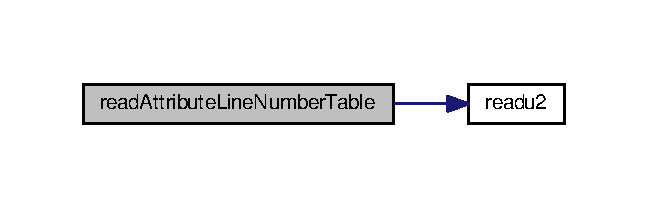
\includegraphics[width=311pt]{attributes_8c_a837af1196cf968ff688539be299648d5_cgraph}
\end{center}
\end{figure}


\index{attributes.\+c@{attributes.\+c}!read\+Attribute\+Source\+File@{read\+Attribute\+Source\+File}}
\index{read\+Attribute\+Source\+File@{read\+Attribute\+Source\+File}!attributes.\+c@{attributes.\+c}}
\subsubsection[{\texorpdfstring{read\+Attribute\+Source\+File(\+Java\+Class $\ast$jc, attribute\+\_\+info $\ast$entry)}{readAttributeSourceFile(JavaClass *jc, attribute_info *entry)}}]{\setlength{\rightskip}{0pt plus 5cm}uint8\+\_\+t read\+Attribute\+Source\+File (
\begin{DoxyParamCaption}
\item[{{\bf Java\+Class} $\ast$}]{jc, }
\item[{{\bf attribute\+\_\+info} $\ast$}]{entry}
\end{DoxyParamCaption}
)}\hypertarget{attributes_8c_a43bfb8cf040e623ccae73943a943a7f8}{}\label{attributes_8c_a43bfb8cf040e623ccae73943a943a7f8}


Here is the call graph for this function\+:\nopagebreak
\begin{figure}[H]
\begin{center}
\leavevmode
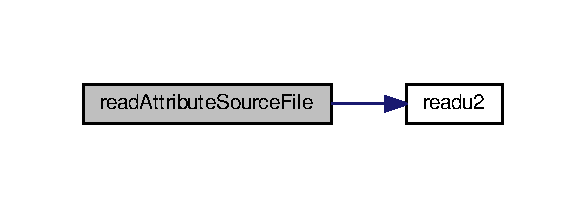
\includegraphics[width=281pt]{attributes_8c_a43bfb8cf040e623ccae73943a943a7f8_cgraph}
\end{center}
\end{figure}



\hypertarget{attributes_8h}{}\section{src/attributes.h File Reference}
\label{attributes_8h}\index{src/attributes.\+h@{src/attributes.\+h}}
{\ttfamily \#include $<$stdint.\+h$>$}\\*
{\ttfamily \#include \char`\"{}javaclass.\+h\char`\"{}}\\*
Include dependency graph for attributes.\+h\+:\nopagebreak
\begin{figure}[H]
\begin{center}
\leavevmode
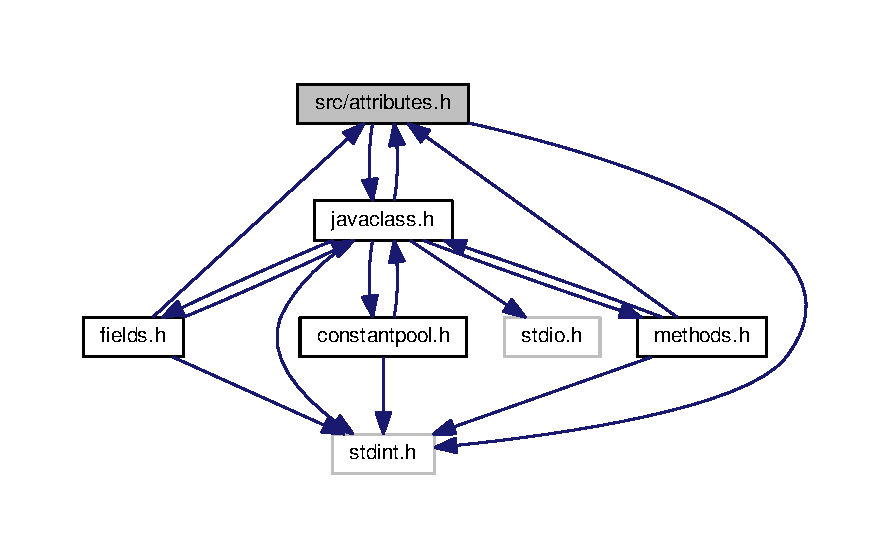
\includegraphics[width=350pt]{attributes_8h__incl}
\end{center}
\end{figure}
This graph shows which files directly or indirectly include this file\+:\nopagebreak
\begin{figure}[H]
\begin{center}
\leavevmode
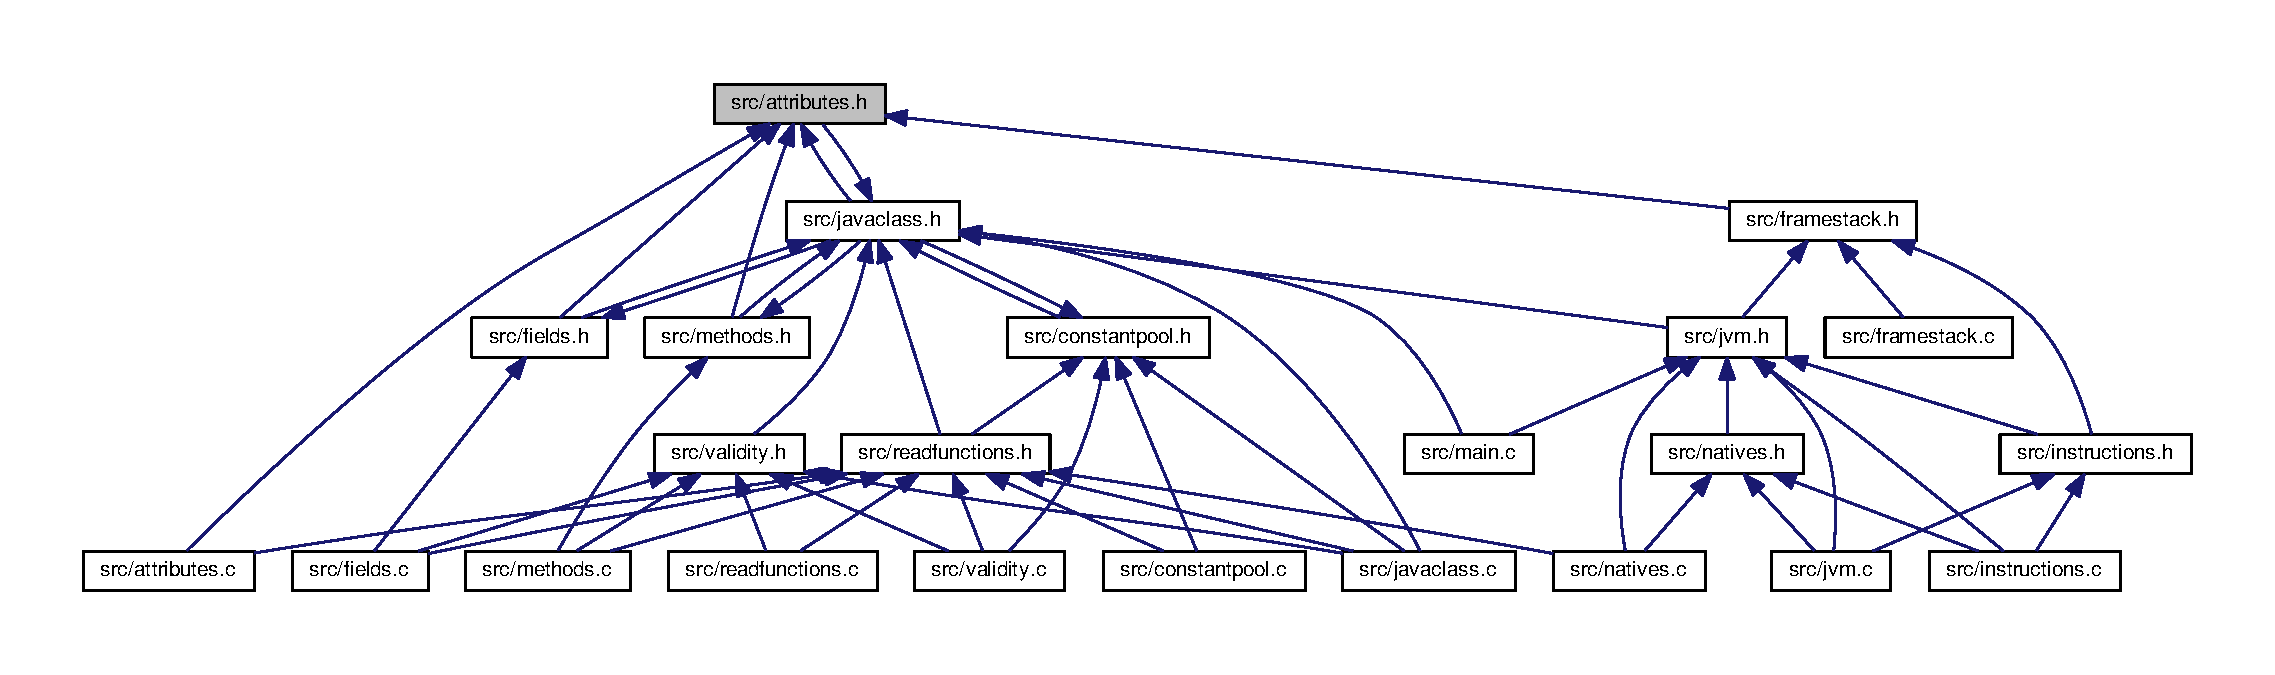
\includegraphics[width=350pt]{attributes_8h__dep__incl}
\end{center}
\end{figure}
\subsection*{Data Structures}
\begin{DoxyCompactItemize}
\item 
struct \hyperlink{structattribute__info}{attribute\+\_\+info}
\item 
struct \hyperlink{structatt__SourceFile__info}{att\+\_\+\+Source\+File\+\_\+info}
\item 
struct \hyperlink{structatt__ConstantValue__info}{att\+\_\+\+Constant\+Value\+\_\+info}
\item 
struct \hyperlink{structInnerClassInfo}{Inner\+Class\+Info}
\item 
struct \hyperlink{structatt__InnerClasses__info}{att\+\_\+\+Inner\+Classes\+\_\+info}
\item 
struct \hyperlink{structLineNumberTableEntry}{Line\+Number\+Table\+Entry}
\item 
struct \hyperlink{structatt__LineNumberTable__info}{att\+\_\+\+Line\+Number\+Table\+\_\+info}
\item 
struct \hyperlink{structExceptionTableEntry}{Exception\+Table\+Entry}
\item 
struct \hyperlink{structatt__Code__info}{att\+\_\+\+Code\+\_\+info}
\item 
struct \hyperlink{structatt__Exceptions__info}{att\+\_\+\+Exceptions\+\_\+info}
\end{DoxyCompactItemize}
\subsection*{Typedefs}
\begin{DoxyCompactItemize}
\item 
typedef struct \hyperlink{structattribute__info}{attribute\+\_\+info} \hyperlink{attributes_8h_a7b1e7b81c7ca3b550a1973f2d8672950}{attribute\+\_\+info}
\end{DoxyCompactItemize}
\subsection*{Enumerations}
\begin{DoxyCompactItemize}
\item 
enum \hyperlink{attributes_8h_a349a9cde14be8097df865ba0469c0ab2}{Attribute\+Type} \{ \\*
\hyperlink{attributes_8h_a349a9cde14be8097df865ba0469c0ab2a84368a0bd5b017d16829889f6fc586b8}{A\+T\+T\+R\+\_\+\+Unknown} = 0, 
\hyperlink{attributes_8h_a349a9cde14be8097df865ba0469c0ab2a48c63d4adab3bf466ab67ee39155bf89}{A\+T\+T\+R\+\_\+\+Constant\+Value}, 
\hyperlink{attributes_8h_a349a9cde14be8097df865ba0469c0ab2a82e29efd5d3c5c77fabf5997ff6da5c2}{A\+T\+T\+R\+\_\+\+Source\+File}, 
\hyperlink{attributes_8h_a349a9cde14be8097df865ba0469c0ab2aa1e111a1adfd4ce3ae583df564a90e09}{A\+T\+T\+R\+\_\+\+Inner\+Classes}, 
\\*
\hyperlink{attributes_8h_a349a9cde14be8097df865ba0469c0ab2a6b8593cf0987a37a80a03e197299597e}{A\+T\+T\+R\+\_\+\+Code}, 
\hyperlink{attributes_8h_a349a9cde14be8097df865ba0469c0ab2a3a2254220839b1156d1eb800f1035e66}{A\+T\+T\+R\+\_\+\+Line\+Number\+Table}, 
\hyperlink{attributes_8h_a349a9cde14be8097df865ba0469c0ab2aa75264de718d1ea76625fb8236133d61}{A\+T\+T\+R\+\_\+\+Exceptions}, 
\hyperlink{attributes_8h_a349a9cde14be8097df865ba0469c0ab2aa8687d6c4b71efe81907687ed84d103a}{A\+T\+T\+R\+\_\+\+Deprecated}
 \}
\end{DoxyCompactItemize}
\subsection*{Functions}
\begin{DoxyCompactItemize}
\item 
char \hyperlink{attributes_8h_a0aab7731ade76c16c2ff8b3bef1111d1}{read\+Attribute} (\hyperlink{structJavaClass}{Java\+Class} $\ast$jc, \hyperlink{structattribute__info}{attribute\+\_\+info} $\ast$entry)
\item 
void \hyperlink{attributes_8h_a136bdfadd787ebd62f1c721f99270cc9}{free\+Attribute\+Info} (\hyperlink{structattribute__info}{attribute\+\_\+info} $\ast$entry)
\item 
void \hyperlink{attributes_8h_aee295c33031c2ab941c9260654010db7}{print\+Attribute} (\hyperlink{structJavaClass}{Java\+Class} $\ast$jc, \hyperlink{structattribute__info}{attribute\+\_\+info} $\ast$entry, int identation\+Level)
\item 
void \hyperlink{attributes_8h_ae04e26b66957c879139f8a82e463674a}{print\+All\+Attributes} (\hyperlink{structJavaClass}{Java\+Class} $\ast$jc)
\item 
\hyperlink{structattribute__info}{attribute\+\_\+info} $\ast$ \hyperlink{attributes_8h_ae3ce1b33741046741c90a6f5592911a5}{get\+Attribute\+By\+Type} (\hyperlink{structattribute__info}{attribute\+\_\+info} $\ast$attributes, uint16\+\_\+t attributes\+\_\+length, enum \hyperlink{attributes_8h_a349a9cde14be8097df865ba0469c0ab2}{Attribute\+Type} type)
\end{DoxyCompactItemize}


\subsection{Typedef Documentation}
\index{attributes.\+h@{attributes.\+h}!attribute\+\_\+info@{attribute\+\_\+info}}
\index{attribute\+\_\+info@{attribute\+\_\+info}!attributes.\+h@{attributes.\+h}}
\subsubsection[{\texorpdfstring{attribute\+\_\+info}{attribute_info}}]{\setlength{\rightskip}{0pt plus 5cm}typedef struct {\bf attribute\+\_\+info} {\bf attribute\+\_\+info}}\hypertarget{attributes_8h_a7b1e7b81c7ca3b550a1973f2d8672950}{}\label{attributes_8h_a7b1e7b81c7ca3b550a1973f2d8672950}


\subsection{Enumeration Type Documentation}
\index{attributes.\+h@{attributes.\+h}!Attribute\+Type@{Attribute\+Type}}
\index{Attribute\+Type@{Attribute\+Type}!attributes.\+h@{attributes.\+h}}
\subsubsection[{\texorpdfstring{Attribute\+Type}{AttributeType}}]{\setlength{\rightskip}{0pt plus 5cm}enum {\bf Attribute\+Type}}\hypertarget{attributes_8h_a349a9cde14be8097df865ba0469c0ab2}{}\label{attributes_8h_a349a9cde14be8097df865ba0469c0ab2}
\begin{Desc}
\item[Enumerator]\par
\begin{description}
\index{A\+T\+T\+R\+\_\+\+Unknown@{A\+T\+T\+R\+\_\+\+Unknown}!attributes.\+h@{attributes.\+h}}\index{attributes.\+h@{attributes.\+h}!A\+T\+T\+R\+\_\+\+Unknown@{A\+T\+T\+R\+\_\+\+Unknown}}\item[{\em 
A\+T\+T\+R\+\_\+\+Unknown\hypertarget{attributes_8h_a349a9cde14be8097df865ba0469c0ab2a84368a0bd5b017d16829889f6fc586b8}{}\label{attributes_8h_a349a9cde14be8097df865ba0469c0ab2a84368a0bd5b017d16829889f6fc586b8}
}]\index{A\+T\+T\+R\+\_\+\+Constant\+Value@{A\+T\+T\+R\+\_\+\+Constant\+Value}!attributes.\+h@{attributes.\+h}}\index{attributes.\+h@{attributes.\+h}!A\+T\+T\+R\+\_\+\+Constant\+Value@{A\+T\+T\+R\+\_\+\+Constant\+Value}}\item[{\em 
A\+T\+T\+R\+\_\+\+Constant\+Value\hypertarget{attributes_8h_a349a9cde14be8097df865ba0469c0ab2a48c63d4adab3bf466ab67ee39155bf89}{}\label{attributes_8h_a349a9cde14be8097df865ba0469c0ab2a48c63d4adab3bf466ab67ee39155bf89}
}]\index{A\+T\+T\+R\+\_\+\+Source\+File@{A\+T\+T\+R\+\_\+\+Source\+File}!attributes.\+h@{attributes.\+h}}\index{attributes.\+h@{attributes.\+h}!A\+T\+T\+R\+\_\+\+Source\+File@{A\+T\+T\+R\+\_\+\+Source\+File}}\item[{\em 
A\+T\+T\+R\+\_\+\+Source\+File\hypertarget{attributes_8h_a349a9cde14be8097df865ba0469c0ab2a82e29efd5d3c5c77fabf5997ff6da5c2}{}\label{attributes_8h_a349a9cde14be8097df865ba0469c0ab2a82e29efd5d3c5c77fabf5997ff6da5c2}
}]\index{A\+T\+T\+R\+\_\+\+Inner\+Classes@{A\+T\+T\+R\+\_\+\+Inner\+Classes}!attributes.\+h@{attributes.\+h}}\index{attributes.\+h@{attributes.\+h}!A\+T\+T\+R\+\_\+\+Inner\+Classes@{A\+T\+T\+R\+\_\+\+Inner\+Classes}}\item[{\em 
A\+T\+T\+R\+\_\+\+Inner\+Classes\hypertarget{attributes_8h_a349a9cde14be8097df865ba0469c0ab2aa1e111a1adfd4ce3ae583df564a90e09}{}\label{attributes_8h_a349a9cde14be8097df865ba0469c0ab2aa1e111a1adfd4ce3ae583df564a90e09}
}]\index{A\+T\+T\+R\+\_\+\+Code@{A\+T\+T\+R\+\_\+\+Code}!attributes.\+h@{attributes.\+h}}\index{attributes.\+h@{attributes.\+h}!A\+T\+T\+R\+\_\+\+Code@{A\+T\+T\+R\+\_\+\+Code}}\item[{\em 
A\+T\+T\+R\+\_\+\+Code\hypertarget{attributes_8h_a349a9cde14be8097df865ba0469c0ab2a6b8593cf0987a37a80a03e197299597e}{}\label{attributes_8h_a349a9cde14be8097df865ba0469c0ab2a6b8593cf0987a37a80a03e197299597e}
}]\index{A\+T\+T\+R\+\_\+\+Line\+Number\+Table@{A\+T\+T\+R\+\_\+\+Line\+Number\+Table}!attributes.\+h@{attributes.\+h}}\index{attributes.\+h@{attributes.\+h}!A\+T\+T\+R\+\_\+\+Line\+Number\+Table@{A\+T\+T\+R\+\_\+\+Line\+Number\+Table}}\item[{\em 
A\+T\+T\+R\+\_\+\+Line\+Number\+Table\hypertarget{attributes_8h_a349a9cde14be8097df865ba0469c0ab2a3a2254220839b1156d1eb800f1035e66}{}\label{attributes_8h_a349a9cde14be8097df865ba0469c0ab2a3a2254220839b1156d1eb800f1035e66}
}]\index{A\+T\+T\+R\+\_\+\+Exceptions@{A\+T\+T\+R\+\_\+\+Exceptions}!attributes.\+h@{attributes.\+h}}\index{attributes.\+h@{attributes.\+h}!A\+T\+T\+R\+\_\+\+Exceptions@{A\+T\+T\+R\+\_\+\+Exceptions}}\item[{\em 
A\+T\+T\+R\+\_\+\+Exceptions\hypertarget{attributes_8h_a349a9cde14be8097df865ba0469c0ab2aa75264de718d1ea76625fb8236133d61}{}\label{attributes_8h_a349a9cde14be8097df865ba0469c0ab2aa75264de718d1ea76625fb8236133d61}
}]\index{A\+T\+T\+R\+\_\+\+Deprecated@{A\+T\+T\+R\+\_\+\+Deprecated}!attributes.\+h@{attributes.\+h}}\index{attributes.\+h@{attributes.\+h}!A\+T\+T\+R\+\_\+\+Deprecated@{A\+T\+T\+R\+\_\+\+Deprecated}}\item[{\em 
A\+T\+T\+R\+\_\+\+Deprecated\hypertarget{attributes_8h_a349a9cde14be8097df865ba0469c0ab2aa8687d6c4b71efe81907687ed84d103a}{}\label{attributes_8h_a349a9cde14be8097df865ba0469c0ab2aa8687d6c4b71efe81907687ed84d103a}
}]\end{description}
\end{Desc}


\subsection{Function Documentation}
\index{attributes.\+h@{attributes.\+h}!free\+Attribute\+Info@{free\+Attribute\+Info}}
\index{free\+Attribute\+Info@{free\+Attribute\+Info}!attributes.\+h@{attributes.\+h}}
\subsubsection[{\texorpdfstring{free\+Attribute\+Info(attribute\+\_\+info $\ast$entry)}{freeAttributeInfo(attribute_info *entry)}}]{\setlength{\rightskip}{0pt plus 5cm}void free\+Attribute\+Info (
\begin{DoxyParamCaption}
\item[{{\bf attribute\+\_\+info} $\ast$}]{entry}
\end{DoxyParamCaption}
)}\hypertarget{attributes_8h_a136bdfadd787ebd62f1c721f99270cc9}{}\label{attributes_8h_a136bdfadd787ebd62f1c721f99270cc9}


Here is the caller graph for this function\+:\nopagebreak
\begin{figure}[H]
\begin{center}
\leavevmode
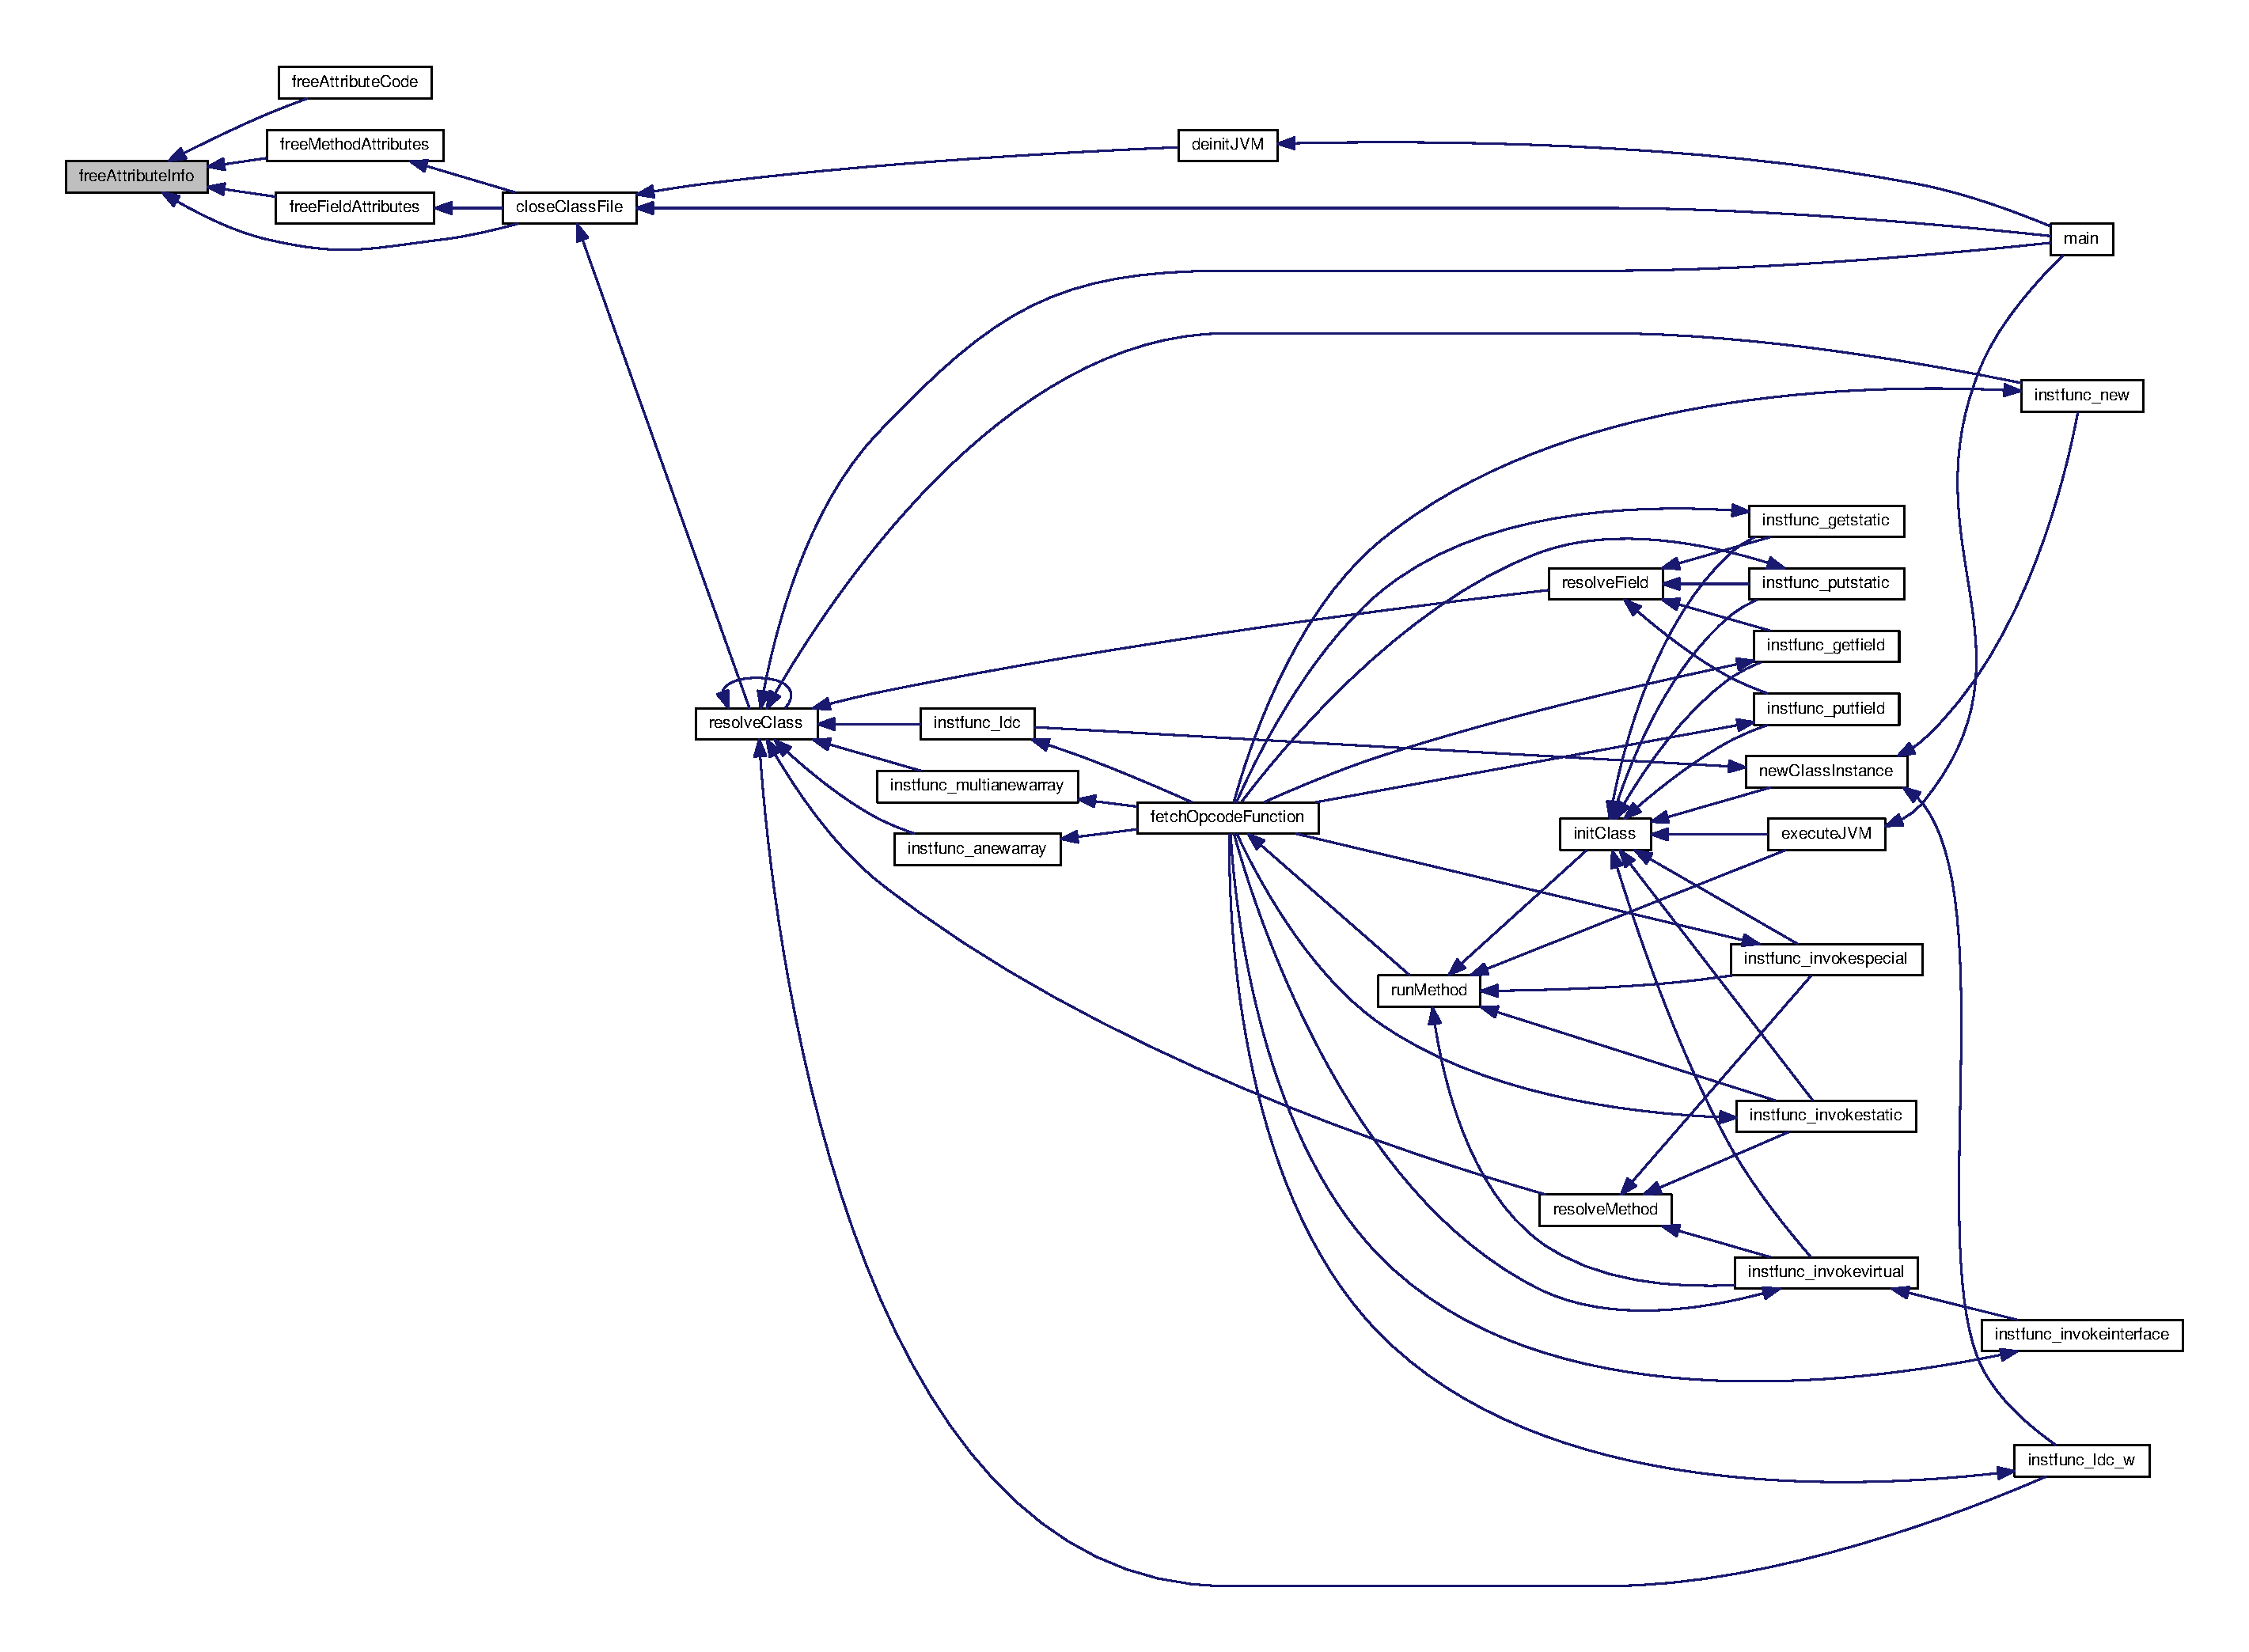
\includegraphics[width=350pt]{attributes_8h_a136bdfadd787ebd62f1c721f99270cc9_icgraph}
\end{center}
\end{figure}


\index{attributes.\+h@{attributes.\+h}!get\+Attribute\+By\+Type@{get\+Attribute\+By\+Type}}
\index{get\+Attribute\+By\+Type@{get\+Attribute\+By\+Type}!attributes.\+h@{attributes.\+h}}
\subsubsection[{\texorpdfstring{get\+Attribute\+By\+Type(attribute\+\_\+info $\ast$attributes, uint16\+\_\+t attributes\+\_\+length, enum Attribute\+Type type)}{getAttributeByType(attribute_info *attributes, uint16_t attributes_length, enum AttributeType type)}}]{\setlength{\rightskip}{0pt plus 5cm}{\bf attribute\+\_\+info}$\ast$ get\+Attribute\+By\+Type (
\begin{DoxyParamCaption}
\item[{{\bf attribute\+\_\+info} $\ast$}]{attributes, }
\item[{uint16\+\_\+t}]{attributes\+\_\+length, }
\item[{enum {\bf Attribute\+Type}}]{type}
\end{DoxyParamCaption}
)}\hypertarget{attributes_8h_ae3ce1b33741046741c90a6f5592911a5}{}\label{attributes_8h_ae3ce1b33741046741c90a6f5592911a5}


Here is the caller graph for this function\+:\nopagebreak
\begin{figure}[H]
\begin{center}
\leavevmode
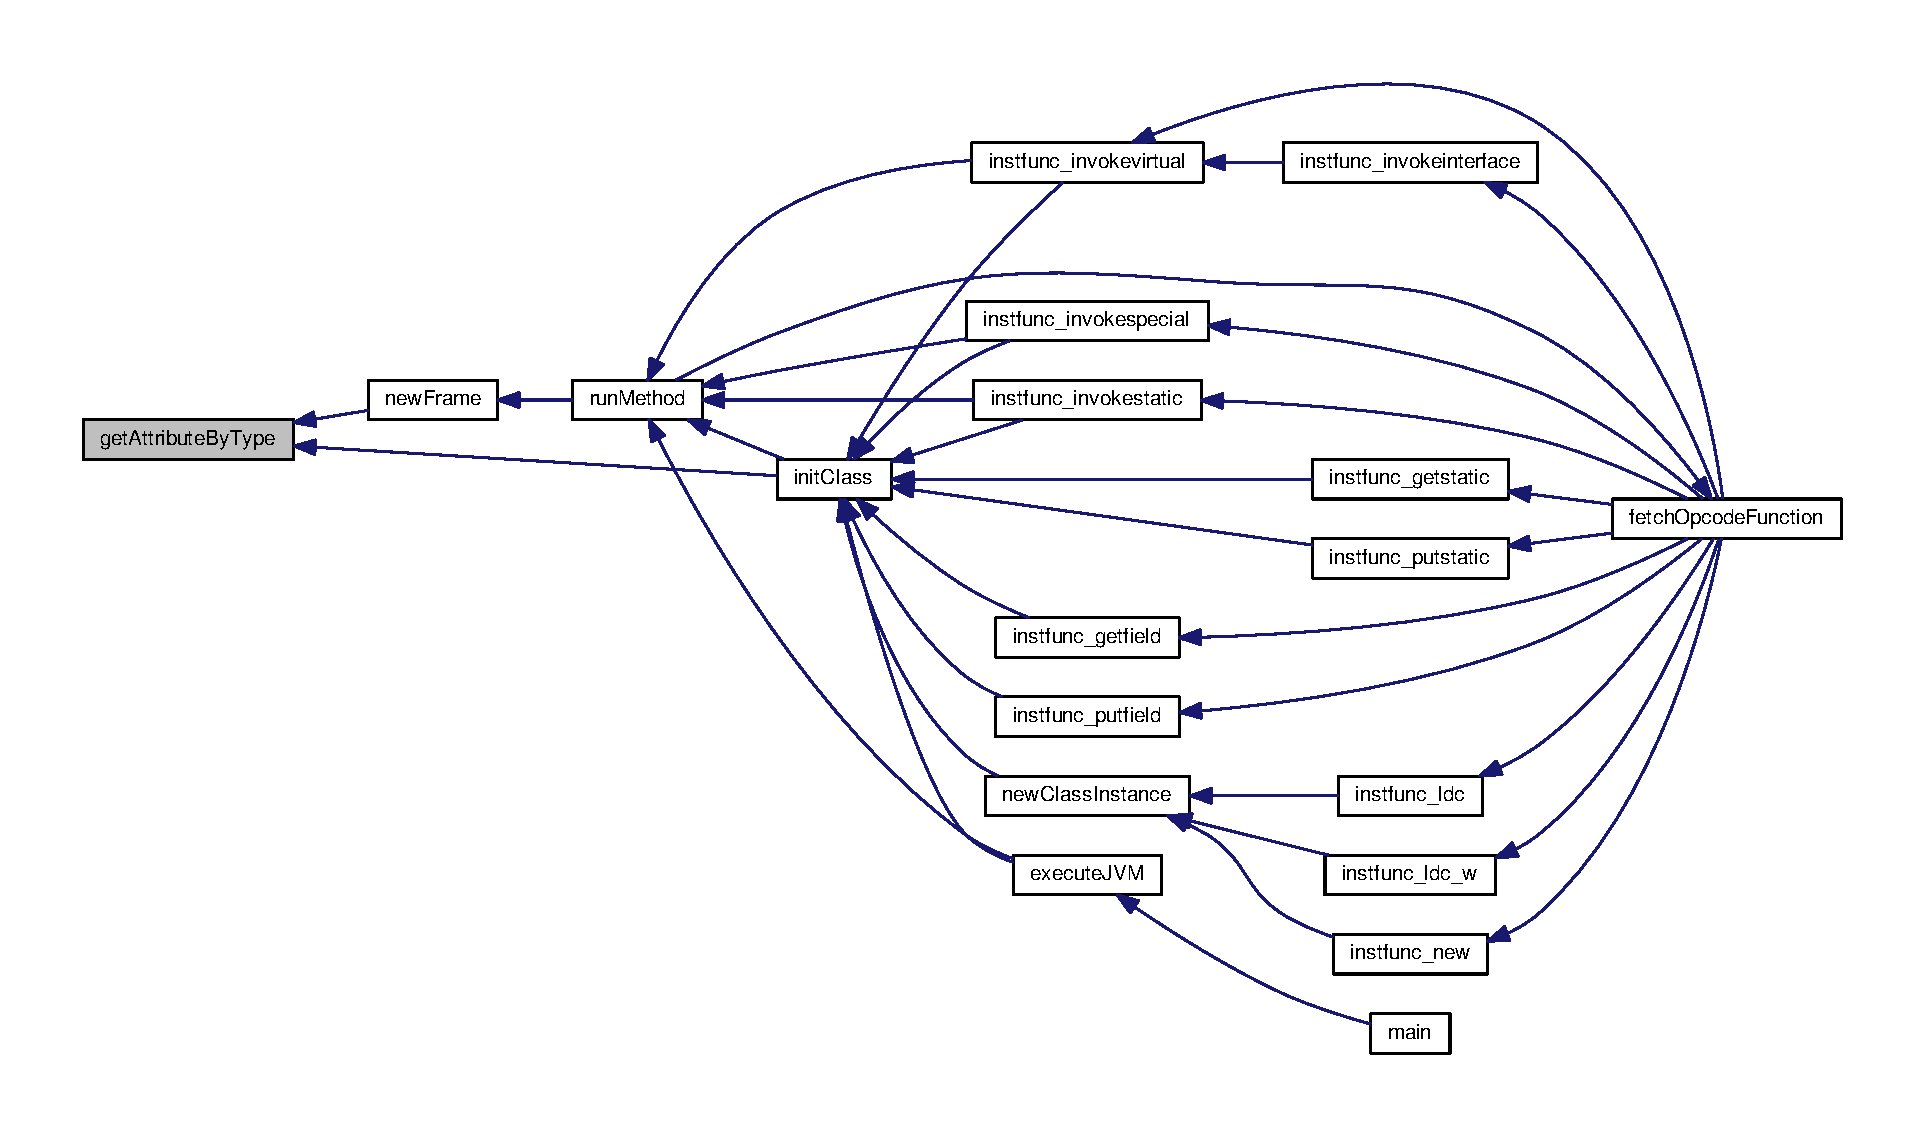
\includegraphics[width=350pt]{attributes_8h_ae3ce1b33741046741c90a6f5592911a5_icgraph}
\end{center}
\end{figure}


\index{attributes.\+h@{attributes.\+h}!print\+All\+Attributes@{print\+All\+Attributes}}
\index{print\+All\+Attributes@{print\+All\+Attributes}!attributes.\+h@{attributes.\+h}}
\subsubsection[{\texorpdfstring{print\+All\+Attributes(\+Java\+Class $\ast$jc)}{printAllAttributes(JavaClass *jc)}}]{\setlength{\rightskip}{0pt plus 5cm}void print\+All\+Attributes (
\begin{DoxyParamCaption}
\item[{{\bf Java\+Class} $\ast$}]{jc}
\end{DoxyParamCaption}
)}\hypertarget{attributes_8h_ae04e26b66957c879139f8a82e463674a}{}\label{attributes_8h_ae04e26b66957c879139f8a82e463674a}


Here is the call graph for this function\+:\nopagebreak
\begin{figure}[H]
\begin{center}
\leavevmode
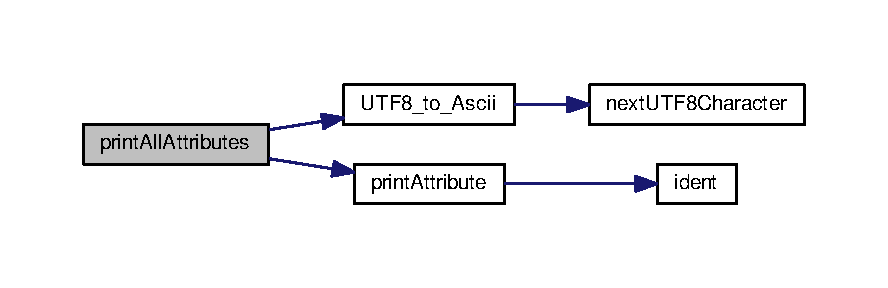
\includegraphics[width=350pt]{attributes_8h_ae04e26b66957c879139f8a82e463674a_cgraph}
\end{center}
\end{figure}




Here is the caller graph for this function\+:\nopagebreak
\begin{figure}[H]
\begin{center}
\leavevmode
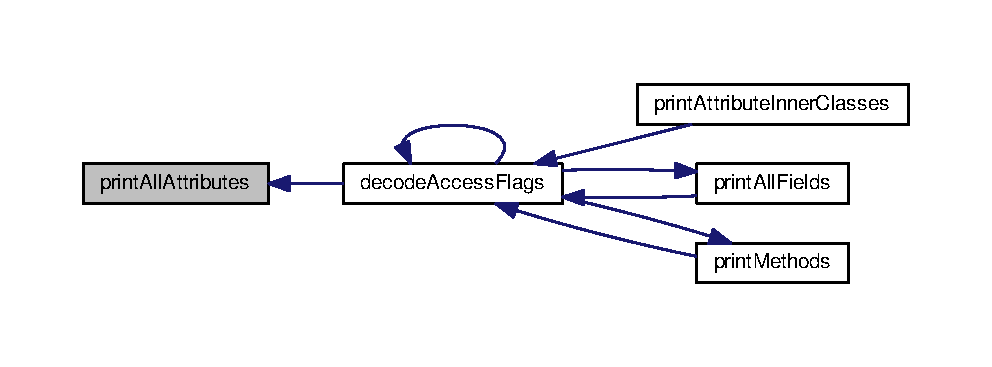
\includegraphics[width=350pt]{attributes_8h_ae04e26b66957c879139f8a82e463674a_icgraph}
\end{center}
\end{figure}


\index{attributes.\+h@{attributes.\+h}!print\+Attribute@{print\+Attribute}}
\index{print\+Attribute@{print\+Attribute}!attributes.\+h@{attributes.\+h}}
\subsubsection[{\texorpdfstring{print\+Attribute(\+Java\+Class $\ast$jc, attribute\+\_\+info $\ast$entry, int identation\+Level)}{printAttribute(JavaClass *jc, attribute_info *entry, int identationLevel)}}]{\setlength{\rightskip}{0pt plus 5cm}void print\+Attribute (
\begin{DoxyParamCaption}
\item[{{\bf Java\+Class} $\ast$}]{jc, }
\item[{{\bf attribute\+\_\+info} $\ast$}]{entry, }
\item[{int}]{identation\+Level}
\end{DoxyParamCaption}
)}\hypertarget{attributes_8h_aee295c33031c2ab941c9260654010db7}{}\label{attributes_8h_aee295c33031c2ab941c9260654010db7}


Here is the call graph for this function\+:\nopagebreak
\begin{figure}[H]
\begin{center}
\leavevmode
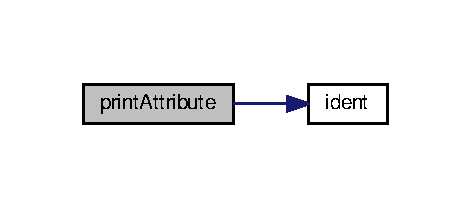
\includegraphics[width=226pt]{attributes_8h_aee295c33031c2ab941c9260654010db7_cgraph}
\end{center}
\end{figure}




Here is the caller graph for this function\+:\nopagebreak
\begin{figure}[H]
\begin{center}
\leavevmode
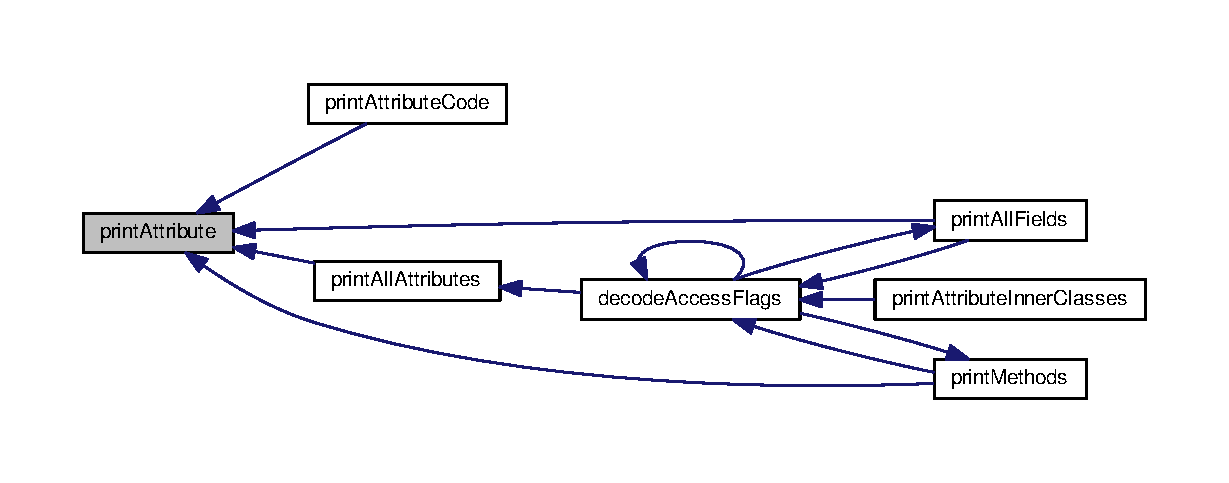
\includegraphics[width=350pt]{attributes_8h_aee295c33031c2ab941c9260654010db7_icgraph}
\end{center}
\end{figure}


\index{attributes.\+h@{attributes.\+h}!read\+Attribute@{read\+Attribute}}
\index{read\+Attribute@{read\+Attribute}!attributes.\+h@{attributes.\+h}}
\subsubsection[{\texorpdfstring{read\+Attribute(\+Java\+Class $\ast$jc, attribute\+\_\+info $\ast$entry)}{readAttribute(JavaClass *jc, attribute_info *entry)}}]{\setlength{\rightskip}{0pt plus 5cm}char read\+Attribute (
\begin{DoxyParamCaption}
\item[{{\bf Java\+Class} $\ast$}]{jc, }
\item[{{\bf attribute\+\_\+info} $\ast$}]{entry}
\end{DoxyParamCaption}
)}\hypertarget{attributes_8h_a0aab7731ade76c16c2ff8b3bef1111d1}{}\label{attributes_8h_a0aab7731ade76c16c2ff8b3bef1111d1}


Here is the call graph for this function\+:\nopagebreak
\begin{figure}[H]
\begin{center}
\leavevmode
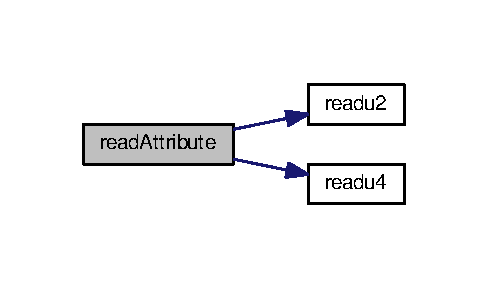
\includegraphics[width=234pt]{attributes_8h_a0aab7731ade76c16c2ff8b3bef1111d1_cgraph}
\end{center}
\end{figure}




Here is the caller graph for this function\+:\nopagebreak
\begin{figure}[H]
\begin{center}
\leavevmode
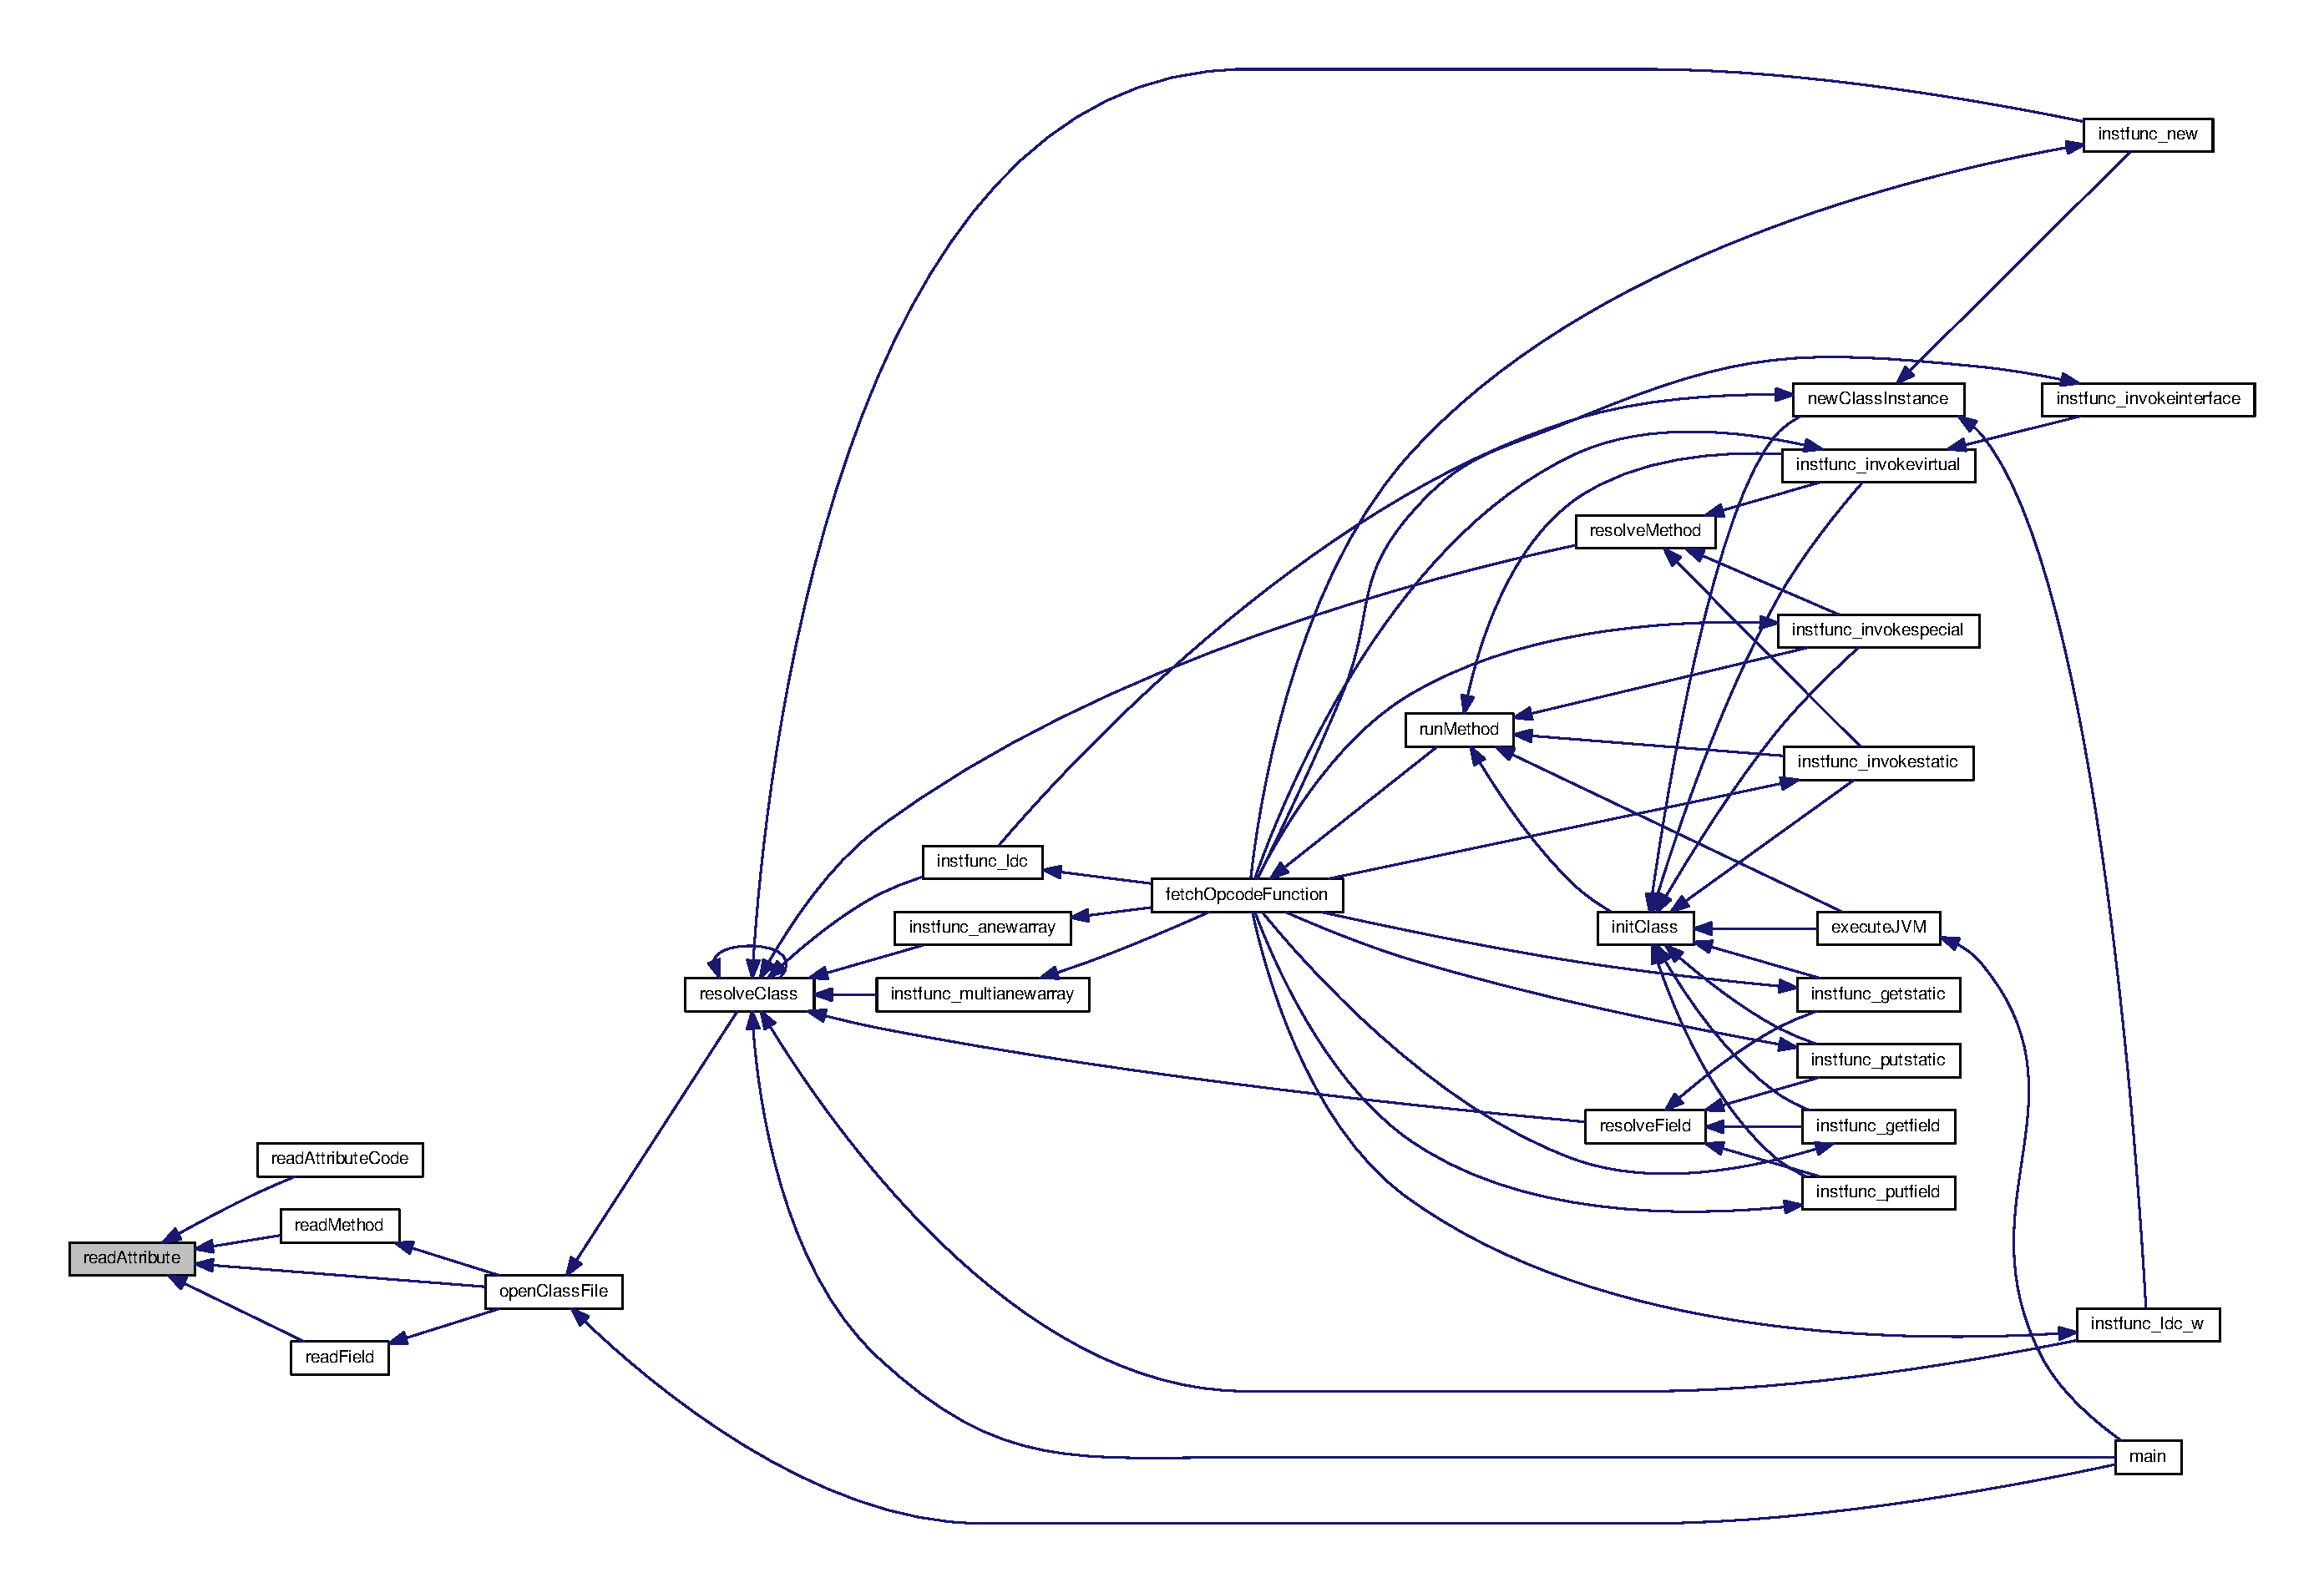
\includegraphics[width=350pt]{attributes_8h_a0aab7731ade76c16c2ff8b3bef1111d1_icgraph}
\end{center}
\end{figure}



\hypertarget{constantpool_8c}{}\section{src/constantpool.c File Reference}
\label{constantpool_8c}\index{src/constantpool.\+c@{src/constantpool.\+c}}
{\ttfamily \#include \char`\"{}debugging.\+h\char`\"{}}\\*
{\ttfamily \#include $<$string.\+h$>$}\\*
{\ttfamily \#include $<$inttypes.\+h$>$}\\*
{\ttfamily \#include \char`\"{}readfunctions.\+h\char`\"{}}\\*
{\ttfamily \#include \char`\"{}constantpool.\+h\char`\"{}}\\*
{\ttfamily \#include \char`\"{}utf8.\+h\char`\"{}}\\*
Include dependency graph for constantpool.\+c\+:\nopagebreak
\begin{figure}[H]
\begin{center}
\leavevmode
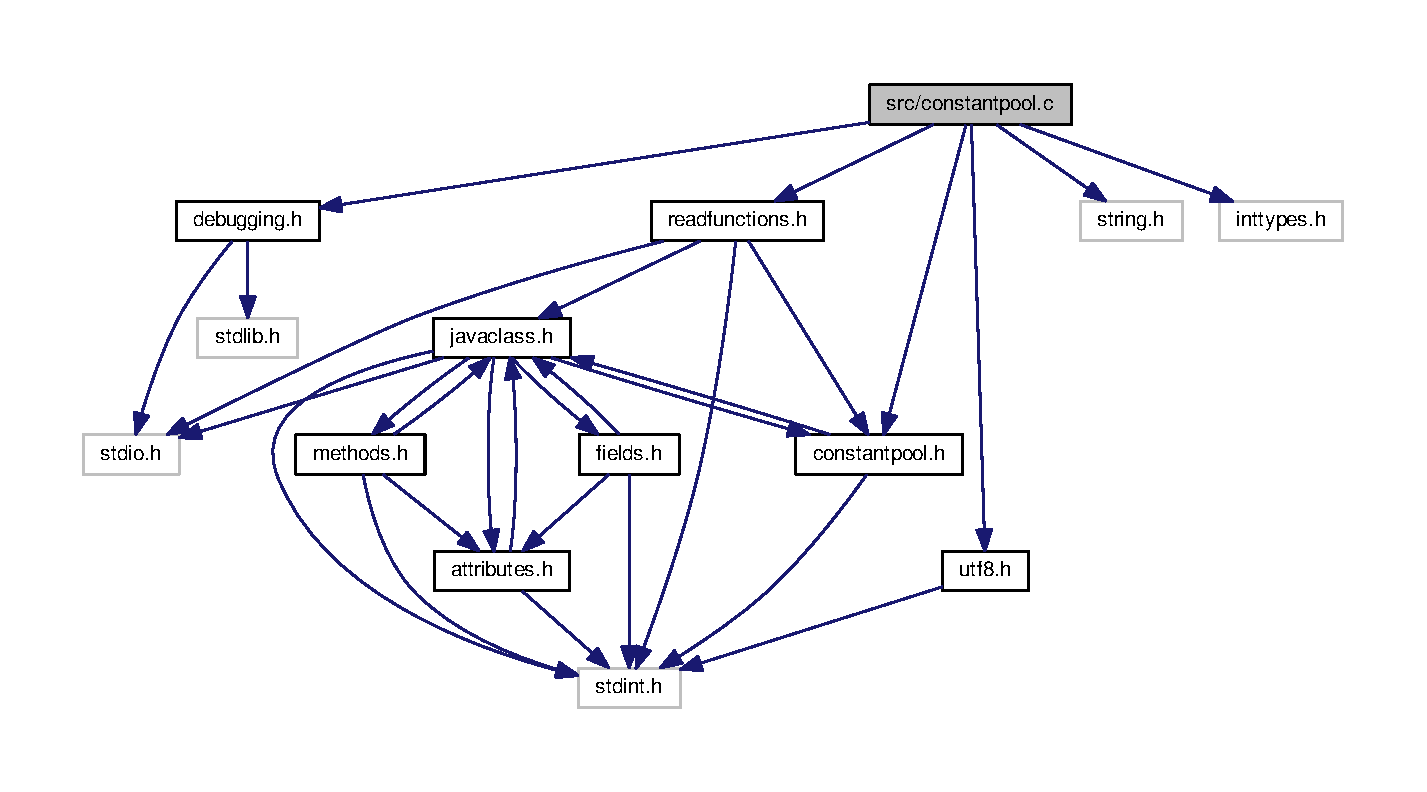
\includegraphics[width=350pt]{constantpool_8c__incl}
\end{center}
\end{figure}
\subsection*{Functions}
\begin{DoxyCompactItemize}
\item 
char \hyperlink{constantpool_8c_afea5409b47477cdbdb590472022c45f9}{read\+Constant\+Pool\+\_\+\+Class} (\hyperlink{structJavaClass}{Java\+Class} $\ast$jc, \hyperlink{structcp__info}{cp\+\_\+info} $\ast$entry)
\begin{DoxyCompactList}\small\item\em Reads a \hyperlink{structcp__info}{cp\+\_\+info} of type C\+O\+N\+S\+T\+A\+N\+T\+\_\+\+Class from the file. \end{DoxyCompactList}\item 
char \hyperlink{constantpool_8c_ab3d1d9a9bdb1b7162d341ce9c8fd8784}{read\+Constant\+Pool\+\_\+\+Fieldref} (\hyperlink{structJavaClass}{Java\+Class} $\ast$jc, \hyperlink{structcp__info}{cp\+\_\+info} $\ast$entry)
\begin{DoxyCompactList}\small\item\em Reads a \hyperlink{structcp__info}{cp\+\_\+info} of type C\+O\+N\+S\+T\+A\+N\+T\+\_\+\+Fieldref from the file. \end{DoxyCompactList}\item 
char \hyperlink{constantpool_8c_a73f94285fc7c4790ca2900b6fc78b0f3}{read\+Constant\+Pool\+\_\+\+Integer} (\hyperlink{structJavaClass}{Java\+Class} $\ast$jc, \hyperlink{structcp__info}{cp\+\_\+info} $\ast$entry)
\begin{DoxyCompactList}\small\item\em Reads a \hyperlink{structcp__info}{cp\+\_\+info} of type C\+O\+N\+S\+T\+A\+N\+T\+\_\+\+Integer from the file. \end{DoxyCompactList}\item 
char \hyperlink{constantpool_8c_a1f4a6c4da0269e609a18f2d8174a2c39}{read\+Constant\+Pool\+\_\+\+Long} (\hyperlink{structJavaClass}{Java\+Class} $\ast$jc, \hyperlink{structcp__info}{cp\+\_\+info} $\ast$entry)
\begin{DoxyCompactList}\small\item\em Reads a \hyperlink{structcp__info}{cp\+\_\+info} of type C\+O\+N\+S\+T\+A\+N\+T\+\_\+\+Long from the file. \end{DoxyCompactList}\item 
char \hyperlink{constantpool_8c_a730bf0dfa0b00508ed8ed3b6119853c3}{read\+Constant\+Pool\+\_\+\+Utf8} (\hyperlink{structJavaClass}{Java\+Class} $\ast$jc, \hyperlink{structcp__info}{cp\+\_\+info} $\ast$entry)
\begin{DoxyCompactList}\small\item\em Reads a \hyperlink{structcp__info}{cp\+\_\+info} of type C\+O\+N\+S\+T\+A\+N\+T\+\_\+\+Utf8 from the file. \end{DoxyCompactList}\item 
char \hyperlink{constantpool_8c_a62504539fde83f5183d20f262d4b1943}{read\+Constant\+Pool\+Entry} (\hyperlink{structJavaClass}{Java\+Class} $\ast$jc, \hyperlink{structcp__info}{cp\+\_\+info} $\ast$entry)
\begin{DoxyCompactList}\small\item\em Reads a \hyperlink{structcp__info}{cp\+\_\+info} from the file. \end{DoxyCompactList}\item 
const char $\ast$ \hyperlink{constantpool_8c_a80f31089353a0ed2d861401c2c741701}{decode\+Tag} (uint8\+\_\+t tag)
\begin{DoxyCompactList}\small\item\em Decodes Constant\+Pool\+Tag enumeration elements. \end{DoxyCompactList}\item 
void \hyperlink{constantpool_8c_a507c6272d8116f956bc75820b2c6ed23}{print\+Constant\+Pool\+Entry} (\hyperlink{structJavaClass}{Java\+Class} $\ast$jc, \hyperlink{structcp__info}{cp\+\_\+info} $\ast$entry)
\begin{DoxyCompactList}\small\item\em Print one single constant from the constant pool. \end{DoxyCompactList}\item 
void \hyperlink{constantpool_8c_ab7d27eb8d4164ae1a1fd11664ba4d1ef}{print\+Constant\+Pool} (\hyperlink{structJavaClass}{Java\+Class} $\ast$jc)
\begin{DoxyCompactList}\small\item\em Function to print all the constants from the constant pool of the class file. \end{DoxyCompactList}\end{DoxyCompactItemize}


\subsection{Function Documentation}
\index{constantpool.\+c@{constantpool.\+c}!decode\+Tag@{decode\+Tag}}
\index{decode\+Tag@{decode\+Tag}!constantpool.\+c@{constantpool.\+c}}
\subsubsection[{\texorpdfstring{decode\+Tag(uint8\+\_\+t tag)}{decodeTag(uint8_t tag)}}]{\setlength{\rightskip}{0pt plus 5cm}const char$\ast$ decode\+Tag (
\begin{DoxyParamCaption}
\item[{uint8\+\_\+t}]{tag}
\end{DoxyParamCaption}
)}\hypertarget{constantpool_8c_a80f31089353a0ed2d861401c2c741701}{}\label{constantpool_8c_a80f31089353a0ed2d861401c2c741701}


Decodes Constant\+Pool\+Tag enumeration elements. 


\begin{DoxyParams}{Parameters}
{\em uint8\+\_\+t} & tag -\/ identifier of the enumeration to be translated.\\
\hline
\end{DoxyParams}
\begin{DoxyReturn}{Returns}
const char$\ast$ -\/ pointer to char containing the decoded tag 
\end{DoxyReturn}


Here is the caller graph for this function\+:\nopagebreak
\begin{figure}[H]
\begin{center}
\leavevmode
\includegraphics[width=350pt]{constantpool_8c_a80f31089353a0ed2d861401c2c741701_icgraph}
\end{center}
\end{figure}


\index{constantpool.\+c@{constantpool.\+c}!print\+Constant\+Pool@{print\+Constant\+Pool}}
\index{print\+Constant\+Pool@{print\+Constant\+Pool}!constantpool.\+c@{constantpool.\+c}}
\subsubsection[{\texorpdfstring{print\+Constant\+Pool(\+Java\+Class $\ast$jc)}{printConstantPool(JavaClass *jc)}}]{\setlength{\rightskip}{0pt plus 5cm}void print\+Constant\+Pool (
\begin{DoxyParamCaption}
\item[{{\bf Java\+Class} $\ast$}]{jc}
\end{DoxyParamCaption}
)}\hypertarget{constantpool_8c_ab7d27eb8d4164ae1a1fd11664ba4d1ef}{}\label{constantpool_8c_ab7d27eb8d4164ae1a1fd11664ba4d1ef}


Function to print all the constants from the constant pool of the class file. 


\begin{DoxyParams}{Parameters}
{\em \hyperlink{structJavaClass}{Java\+Class}} & $\ast$jc -\/ pointer to \hyperlink{structJavaClass}{Java\+Class} structure that must already be loaded \\
\hline
\end{DoxyParams}


Here is the call graph for this function\+:\nopagebreak
\begin{figure}[H]
\begin{center}
\leavevmode
\includegraphics[width=350pt]{constantpool_8c_ab7d27eb8d4164ae1a1fd11664ba4d1ef_cgraph}
\end{center}
\end{figure}




Here is the caller graph for this function\+:\nopagebreak
\begin{figure}[H]
\begin{center}
\leavevmode
\includegraphics[width=350pt]{constantpool_8c_ab7d27eb8d4164ae1a1fd11664ba4d1ef_icgraph}
\end{center}
\end{figure}


\index{constantpool.\+c@{constantpool.\+c}!print\+Constant\+Pool\+Entry@{print\+Constant\+Pool\+Entry}}
\index{print\+Constant\+Pool\+Entry@{print\+Constant\+Pool\+Entry}!constantpool.\+c@{constantpool.\+c}}
\subsubsection[{\texorpdfstring{print\+Constant\+Pool\+Entry(\+Java\+Class $\ast$jc, cp\+\_\+info $\ast$entry)}{printConstantPoolEntry(JavaClass *jc, cp_info *entry)}}]{\setlength{\rightskip}{0pt plus 5cm}void print\+Constant\+Pool\+Entry (
\begin{DoxyParamCaption}
\item[{{\bf Java\+Class} $\ast$}]{jc, }
\item[{{\bf cp\+\_\+info} $\ast$}]{entry}
\end{DoxyParamCaption}
)}\hypertarget{constantpool_8c_a507c6272d8116f956bc75820b2c6ed23}{}\label{constantpool_8c_a507c6272d8116f956bc75820b2c6ed23}


Print one single constant from the constant pool. 


\begin{DoxyParams}{Parameters}
{\em Java\+Class$\ast$} & jc -\/ pointer to \hyperlink{structJavaClass}{Java\+Class} structure that must already be loaded, no checks are made. \\
\hline
{\em $\ast$entry} & -\/ the pointer to the constant that will be printed. \\
\hline
\end{DoxyParams}


Here is the call graph for this function\+:\nopagebreak
\begin{figure}[H]
\begin{center}
\leavevmode
\includegraphics[width=350pt]{constantpool_8c_a507c6272d8116f956bc75820b2c6ed23_cgraph}
\end{center}
\end{figure}




Here is the caller graph for this function\+:\nopagebreak
\begin{figure}[H]
\begin{center}
\leavevmode
\includegraphics[width=350pt]{constantpool_8c_a507c6272d8116f956bc75820b2c6ed23_icgraph}
\end{center}
\end{figure}


\index{constantpool.\+c@{constantpool.\+c}!read\+Constant\+Pool\+\_\+\+Class@{read\+Constant\+Pool\+\_\+\+Class}}
\index{read\+Constant\+Pool\+\_\+\+Class@{read\+Constant\+Pool\+\_\+\+Class}!constantpool.\+c@{constantpool.\+c}}
\subsubsection[{\texorpdfstring{read\+Constant\+Pool\+\_\+\+Class(\+Java\+Class $\ast$jc, cp\+\_\+info $\ast$entry)}{readConstantPool_Class(JavaClass *jc, cp_info *entry)}}]{\setlength{\rightskip}{0pt plus 5cm}char read\+Constant\+Pool\+\_\+\+Class (
\begin{DoxyParamCaption}
\item[{{\bf Java\+Class} $\ast$}]{jc, }
\item[{{\bf cp\+\_\+info} $\ast$}]{entry}
\end{DoxyParamCaption}
)}\hypertarget{constantpool_8c_afea5409b47477cdbdb590472022c45f9}{}\label{constantpool_8c_afea5409b47477cdbdb590472022c45f9}


Reads a \hyperlink{structcp__info}{cp\+\_\+info} of type C\+O\+N\+S\+T\+A\+N\+T\+\_\+\+Class from the file. 

Reads a \hyperlink{structcp__info}{cp\+\_\+info} of type C\+O\+N\+S\+T\+A\+N\+T\+\_\+\+Class from the file Data read is written to pointer $\ast$entry. C\+O\+N\+S\+T\+A\+N\+T\+\_\+\+Class has the same structure as C\+O\+N\+S\+T\+A\+N\+T\+\_\+\+String, so this function could be used to read that too.


\begin{DoxyParams}{Parameters}
{\em Java\+Class$\ast$} & jc -\/ pointer to the structure to be read. \\
\hline
{\em cp\+\_\+info$\ast$} & entry -\/ where the data read is written\\
\hline
\end{DoxyParams}
\begin{DoxyReturn}{Returns}
char -\/ retuns 0 if something unexpected happened or failure, 1 in case of success 
\end{DoxyReturn}


Here is the call graph for this function\+:\nopagebreak
\begin{figure}[H]
\begin{center}
\leavevmode
\includegraphics[width=287pt]{constantpool_8c_afea5409b47477cdbdb590472022c45f9_cgraph}
\end{center}
\end{figure}




Here is the caller graph for this function\+:\nopagebreak
\begin{figure}[H]
\begin{center}
\leavevmode
\includegraphics[width=350pt]{constantpool_8c_afea5409b47477cdbdb590472022c45f9_icgraph}
\end{center}
\end{figure}


\index{constantpool.\+c@{constantpool.\+c}!read\+Constant\+Pool\+\_\+\+Fieldref@{read\+Constant\+Pool\+\_\+\+Fieldref}}
\index{read\+Constant\+Pool\+\_\+\+Fieldref@{read\+Constant\+Pool\+\_\+\+Fieldref}!constantpool.\+c@{constantpool.\+c}}
\subsubsection[{\texorpdfstring{read\+Constant\+Pool\+\_\+\+Fieldref(\+Java\+Class $\ast$jc, cp\+\_\+info $\ast$entry)}{readConstantPool_Fieldref(JavaClass *jc, cp_info *entry)}}]{\setlength{\rightskip}{0pt plus 5cm}char read\+Constant\+Pool\+\_\+\+Fieldref (
\begin{DoxyParamCaption}
\item[{{\bf Java\+Class} $\ast$}]{jc, }
\item[{{\bf cp\+\_\+info} $\ast$}]{entry}
\end{DoxyParamCaption}
)}\hypertarget{constantpool_8c_ab3d1d9a9bdb1b7162d341ce9c8fd8784}{}\label{constantpool_8c_ab3d1d9a9bdb1b7162d341ce9c8fd8784}


Reads a \hyperlink{structcp__info}{cp\+\_\+info} of type C\+O\+N\+S\+T\+A\+N\+T\+\_\+\+Fieldref from the file. 

C\+O\+N\+S\+T\+A\+N\+T\+\_\+\+Fieldref has the same internal structure as C\+O\+N\+S\+T\+A\+N\+T\+\_\+\+Methodref C\+O\+N\+S\+T\+A\+N\+T\+\_\+\+Interface\+Methodref and C\+O\+N\+S\+T\+A\+N\+T\+\_\+\+Name\+And\+Type, so this function can be also used to read those.


\begin{DoxyParams}{Parameters}
{\em Java\+Class$\ast$} & jc -\/ pointer to the structure to be read. \\
\hline
{\em cp\+\_\+info$\ast$} & entry -\/ where the data read is written\\
\hline
\end{DoxyParams}
\begin{DoxyReturn}{Returns}
char -\/ retuns 0 if something unexpected happened or failure, 1 in case of success 
\end{DoxyReturn}


Here is the call graph for this function\+:\nopagebreak
\begin{figure}[H]
\begin{center}
\leavevmode
\includegraphics[width=294pt]{constantpool_8c_ab3d1d9a9bdb1b7162d341ce9c8fd8784_cgraph}
\end{center}
\end{figure}




Here is the caller graph for this function\+:\nopagebreak
\begin{figure}[H]
\begin{center}
\leavevmode
\includegraphics[width=350pt]{constantpool_8c_ab3d1d9a9bdb1b7162d341ce9c8fd8784_icgraph}
\end{center}
\end{figure}


\index{constantpool.\+c@{constantpool.\+c}!read\+Constant\+Pool\+\_\+\+Integer@{read\+Constant\+Pool\+\_\+\+Integer}}
\index{read\+Constant\+Pool\+\_\+\+Integer@{read\+Constant\+Pool\+\_\+\+Integer}!constantpool.\+c@{constantpool.\+c}}
\subsubsection[{\texorpdfstring{read\+Constant\+Pool\+\_\+\+Integer(\+Java\+Class $\ast$jc, cp\+\_\+info $\ast$entry)}{readConstantPool_Integer(JavaClass *jc, cp_info *entry)}}]{\setlength{\rightskip}{0pt plus 5cm}char read\+Constant\+Pool\+\_\+\+Integer (
\begin{DoxyParamCaption}
\item[{{\bf Java\+Class} $\ast$}]{jc, }
\item[{{\bf cp\+\_\+info} $\ast$}]{entry}
\end{DoxyParamCaption}
)}\hypertarget{constantpool_8c_a73f94285fc7c4790ca2900b6fc78b0f3}{}\label{constantpool_8c_a73f94285fc7c4790ca2900b6fc78b0f3}


Reads a \hyperlink{structcp__info}{cp\+\_\+info} of type C\+O\+N\+S\+T\+A\+N\+T\+\_\+\+Integer from the file. 

C\+O\+N\+S\+T\+A\+N\+T\+\_\+\+Integer has the same structure as C\+O\+N\+S\+T\+A\+N\+T\+\_\+\+Float, so this function could be used to read that too.


\begin{DoxyParams}{Parameters}
{\em Java\+Class$\ast$} & jc -\/ pointer to the structure to be read. \\
\hline
{\em cp\+\_\+info$\ast$} & entry -\/ where the data read is written\\
\hline
\end{DoxyParams}
\begin{DoxyReturn}{Returns}
char -\/ retuns 0 if something unexpected happened 1 in case of success 
\end{DoxyReturn}


Here is the call graph for this function\+:\nopagebreak
\begin{figure}[H]
\begin{center}
\leavevmode
\includegraphics[width=292pt]{constantpool_8c_a73f94285fc7c4790ca2900b6fc78b0f3_cgraph}
\end{center}
\end{figure}




Here is the caller graph for this function\+:\nopagebreak
\begin{figure}[H]
\begin{center}
\leavevmode
\includegraphics[width=350pt]{constantpool_8c_a73f94285fc7c4790ca2900b6fc78b0f3_icgraph}
\end{center}
\end{figure}


\index{constantpool.\+c@{constantpool.\+c}!read\+Constant\+Pool\+\_\+\+Long@{read\+Constant\+Pool\+\_\+\+Long}}
\index{read\+Constant\+Pool\+\_\+\+Long@{read\+Constant\+Pool\+\_\+\+Long}!constantpool.\+c@{constantpool.\+c}}
\subsubsection[{\texorpdfstring{read\+Constant\+Pool\+\_\+\+Long(\+Java\+Class $\ast$jc, cp\+\_\+info $\ast$entry)}{readConstantPool_Long(JavaClass *jc, cp_info *entry)}}]{\setlength{\rightskip}{0pt plus 5cm}char read\+Constant\+Pool\+\_\+\+Long (
\begin{DoxyParamCaption}
\item[{{\bf Java\+Class} $\ast$}]{jc, }
\item[{{\bf cp\+\_\+info} $\ast$}]{entry}
\end{DoxyParamCaption}
)}\hypertarget{constantpool_8c_a1f4a6c4da0269e609a18f2d8174a2c39}{}\label{constantpool_8c_a1f4a6c4da0269e609a18f2d8174a2c39}


Reads a \hyperlink{structcp__info}{cp\+\_\+info} of type C\+O\+N\+S\+T\+A\+N\+T\+\_\+\+Long from the file. 

C\+O\+N\+S\+T\+A\+N\+T\+\_\+\+Long has the same structure as C\+O\+N\+S\+T\+A\+N\+T\+\_\+\+Double, so this function could be used to read that too.


\begin{DoxyParams}{Parameters}
{\em Java\+Class$\ast$} & jc -\/ pointer to the structure to be read. \\
\hline
{\em cp\+\_\+info$\ast$} & entry -\/ where the data read is written\\
\hline
\end{DoxyParams}
\begin{DoxyReturn}{Returns}
char -\/ retuns 0 if something unexpected happened or failure, 1 in case of success 
\end{DoxyReturn}


Here is the call graph for this function\+:\nopagebreak
\begin{figure}[H]
\begin{center}
\leavevmode
\includegraphics[width=283pt]{constantpool_8c_a1f4a6c4da0269e609a18f2d8174a2c39_cgraph}
\end{center}
\end{figure}




Here is the caller graph for this function\+:\nopagebreak
\begin{figure}[H]
\begin{center}
\leavevmode
\includegraphics[width=350pt]{constantpool_8c_a1f4a6c4da0269e609a18f2d8174a2c39_icgraph}
\end{center}
\end{figure}


\index{constantpool.\+c@{constantpool.\+c}!read\+Constant\+Pool\+\_\+\+Utf8@{read\+Constant\+Pool\+\_\+\+Utf8}}
\index{read\+Constant\+Pool\+\_\+\+Utf8@{read\+Constant\+Pool\+\_\+\+Utf8}!constantpool.\+c@{constantpool.\+c}}
\subsubsection[{\texorpdfstring{read\+Constant\+Pool\+\_\+\+Utf8(\+Java\+Class $\ast$jc, cp\+\_\+info $\ast$entry)}{readConstantPool_Utf8(JavaClass *jc, cp_info *entry)}}]{\setlength{\rightskip}{0pt plus 5cm}char read\+Constant\+Pool\+\_\+\+Utf8 (
\begin{DoxyParamCaption}
\item[{{\bf Java\+Class} $\ast$}]{jc, }
\item[{{\bf cp\+\_\+info} $\ast$}]{entry}
\end{DoxyParamCaption}
)}\hypertarget{constantpool_8c_a730bf0dfa0b00508ed8ed3b6119853c3}{}\label{constantpool_8c_a730bf0dfa0b00508ed8ed3b6119853c3}


Reads a \hyperlink{structcp__info}{cp\+\_\+info} of type C\+O\+N\+S\+T\+A\+N\+T\+\_\+\+Utf8 from the file. 


\begin{DoxyParams}{Parameters}
{\em Java\+Class$\ast$} & jc -\/ pointer to the structure to be read. \\
\hline
{\em cp\+\_\+info$\ast$} & entry -\/ where the data read is written\\
\hline
\end{DoxyParams}
\begin{DoxyReturn}{Returns}
char -\/ retuns 0 if something unexpected happened or failure, 1 in case of success 
\end{DoxyReturn}


Here is the call graph for this function\+:\nopagebreak
\begin{figure}[H]
\begin{center}
\leavevmode
\includegraphics[width=281pt]{constantpool_8c_a730bf0dfa0b00508ed8ed3b6119853c3_cgraph}
\end{center}
\end{figure}




Here is the caller graph for this function\+:\nopagebreak
\begin{figure}[H]
\begin{center}
\leavevmode
\includegraphics[width=350pt]{constantpool_8c_a730bf0dfa0b00508ed8ed3b6119853c3_icgraph}
\end{center}
\end{figure}


\index{constantpool.\+c@{constantpool.\+c}!read\+Constant\+Pool\+Entry@{read\+Constant\+Pool\+Entry}}
\index{read\+Constant\+Pool\+Entry@{read\+Constant\+Pool\+Entry}!constantpool.\+c@{constantpool.\+c}}
\subsubsection[{\texorpdfstring{read\+Constant\+Pool\+Entry(\+Java\+Class $\ast$jc, cp\+\_\+info $\ast$entry)}{readConstantPoolEntry(JavaClass *jc, cp_info *entry)}}]{\setlength{\rightskip}{0pt plus 5cm}char read\+Constant\+Pool\+Entry (
\begin{DoxyParamCaption}
\item[{{\bf Java\+Class} $\ast$}]{jc, }
\item[{{\bf cp\+\_\+info} $\ast$}]{entry}
\end{DoxyParamCaption}
)}\hypertarget{constantpool_8c_a62504539fde83f5183d20f262d4b1943}{}\label{constantpool_8c_a62504539fde83f5183d20f262d4b1943}


Reads a \hyperlink{structcp__info}{cp\+\_\+info} from the file. 

This function identifies the structure indicated by the tag byte and selects the corresponding reading type


\begin{DoxyParams}{Parameters}
{\em Java\+Class$\ast$} & jc -\/ pointer to the structure to be read. \\
\hline
{\em cp\+\_\+info$\ast$} & entry -\/ where the data read is written\\
\hline
\end{DoxyParams}
\begin{DoxyReturn}{Returns}
char -\/ retuns 0 if something unexpected happened or failure, 1 in case of success 
\end{DoxyReturn}


Here is the call graph for this function\+:\nopagebreak
\begin{figure}[H]
\begin{center}
\leavevmode
\includegraphics[width=350pt]{constantpool_8c_a62504539fde83f5183d20f262d4b1943_cgraph}
\end{center}
\end{figure}




Here is the caller graph for this function\+:\nopagebreak
\begin{figure}[H]
\begin{center}
\leavevmode
\includegraphics[width=350pt]{constantpool_8c_a62504539fde83f5183d20f262d4b1943_icgraph}
\end{center}
\end{figure}



\hypertarget{constantpool_8h}{}\section{src/constantpool.h File Reference}
\label{constantpool_8h}\index{src/constantpool.\+h@{src/constantpool.\+h}}
{\ttfamily \#include $<$stdint.\+h$>$}\\*
{\ttfamily \#include \char`\"{}javaclass.\+h\char`\"{}}\\*
Include dependency graph for constantpool.\+h\+:\nopagebreak
\begin{figure}[H]
\begin{center}
\leavevmode
\includegraphics[width=350pt]{constantpool_8h__incl}
\end{center}
\end{figure}
This graph shows which files directly or indirectly include this file\+:\nopagebreak
\begin{figure}[H]
\begin{center}
\leavevmode
\includegraphics[width=350pt]{constantpool_8h__dep__incl}
\end{center}
\end{figure}
\subsection*{Data Structures}
\begin{DoxyCompactItemize}
\item 
struct \hyperlink{structcp__info}{cp\+\_\+info}
\end{DoxyCompactItemize}
\subsection*{Typedefs}
\begin{DoxyCompactItemize}
\item 
typedef struct \hyperlink{structcp__info}{cp\+\_\+info} \hyperlink{constantpool_8h_ac152ca02fa3b57b8d90f0ae0b30f099a}{cp\+\_\+info}
\end{DoxyCompactItemize}
\subsection*{Enumerations}
\begin{DoxyCompactItemize}
\item 
enum \hyperlink{constantpool_8h_a4a3344c6a9649978cbcf29955d4de3c3}{Constant\+Pool\+Tag} \{ \\*
\hyperlink{constantpool_8h_a4a3344c6a9649978cbcf29955d4de3c3a0c47012a59af298b394855447822a7e3}{C\+O\+N\+S\+T\+A\+N\+T\+\_\+\+Class} = 7, 
\hyperlink{constantpool_8h_a4a3344c6a9649978cbcf29955d4de3c3a6f435c620d73f5e9366149665dc8ec6e}{C\+O\+N\+S\+T\+A\+N\+T\+\_\+\+Fieldref} = 9, 
\hyperlink{constantpool_8h_a4a3344c6a9649978cbcf29955d4de3c3a74af7140e84140c938fbf89e0c33eea8}{C\+O\+N\+S\+T\+A\+N\+T\+\_\+\+Methodref} = 10, 
\hyperlink{constantpool_8h_a4a3344c6a9649978cbcf29955d4de3c3a49962b9b17bc2ab27647a398b8083828}{C\+O\+N\+S\+T\+A\+N\+T\+\_\+\+Interface\+Methodref} = 11, 
\\*
\hyperlink{constantpool_8h_a4a3344c6a9649978cbcf29955d4de3c3a2c4493d41b4f7ff5cf9f2846e1bb92e0}{C\+O\+N\+S\+T\+A\+N\+T\+\_\+\+String} = 8, 
\hyperlink{constantpool_8h_a4a3344c6a9649978cbcf29955d4de3c3a211cf9d5f5f1416862052d4671ad440f}{C\+O\+N\+S\+T\+A\+N\+T\+\_\+\+Integer} = 3, 
\hyperlink{constantpool_8h_a4a3344c6a9649978cbcf29955d4de3c3aaef0ceec2622d1d49b45fbe54e406f21}{C\+O\+N\+S\+T\+A\+N\+T\+\_\+\+Float} = 4, 
\hyperlink{constantpool_8h_a4a3344c6a9649978cbcf29955d4de3c3a1d98ddfe1f9abb18cf43bc2c1b74bdd5}{C\+O\+N\+S\+T\+A\+N\+T\+\_\+\+Long} = 5, 
\\*
\hyperlink{constantpool_8h_a4a3344c6a9649978cbcf29955d4de3c3a728b77a24433c54f6c8a0f613e50a2c5}{C\+O\+N\+S\+T\+A\+N\+T\+\_\+\+Double} = 6, 
\hyperlink{constantpool_8h_a4a3344c6a9649978cbcf29955d4de3c3a80805f21212baf2079b2ab767e2ab061}{C\+O\+N\+S\+T\+A\+N\+T\+\_\+\+Name\+And\+Type} = 12, 
\hyperlink{constantpool_8h_a4a3344c6a9649978cbcf29955d4de3c3a4100a823f09e364338e42951035432ed}{C\+O\+N\+S\+T\+A\+N\+T\+\_\+\+Utf8} = 1, 
\hyperlink{constantpool_8h_a4a3344c6a9649978cbcf29955d4de3c3ac9fdca41420c578c73fadfa67d4ae26a}{C\+O\+N\+S\+T\+A\+N\+T\+\_\+\+Method\+Handle} = 15, 
\\*
\hyperlink{constantpool_8h_a4a3344c6a9649978cbcf29955d4de3c3a52dbe317b7b19ea9d13a8b185842d245}{C\+O\+N\+S\+T\+A\+N\+T\+\_\+\+Method\+Type} = 16, 
\hyperlink{constantpool_8h_a4a3344c6a9649978cbcf29955d4de3c3a914abae8d35d480c7856e97ca4fc00e0}{C\+O\+N\+S\+T\+A\+N\+T\+\_\+\+Invoke\+Dynamic} = 18
 \}
\end{DoxyCompactItemize}
\subsection*{Functions}
\begin{DoxyCompactItemize}
\item 
const char $\ast$ \hyperlink{constantpool_8h_a80f31089353a0ed2d861401c2c741701}{decode\+Tag} (uint8\+\_\+t tag)
\begin{DoxyCompactList}\small\item\em Decodes Constant\+Pool\+Tag enumeration elements. \end{DoxyCompactList}\item 
char \hyperlink{constantpool_8h_a62504539fde83f5183d20f262d4b1943}{read\+Constant\+Pool\+Entry} (\hyperlink{structJavaClass}{Java\+Class} $\ast$jc, \hyperlink{structcp__info}{cp\+\_\+info} $\ast$entry)
\begin{DoxyCompactList}\small\item\em Reads a \hyperlink{structcp__info}{cp\+\_\+info} from the file. \end{DoxyCompactList}\item 
void \hyperlink{constantpool_8h_ab7d27eb8d4164ae1a1fd11664ba4d1ef}{print\+Constant\+Pool} (\hyperlink{structJavaClass}{Java\+Class} $\ast$jc)
\begin{DoxyCompactList}\small\item\em Function to print all the constants from the constant pool of the class file. \end{DoxyCompactList}\end{DoxyCompactItemize}


\subsection{Typedef Documentation}
\index{constantpool.\+h@{constantpool.\+h}!cp\+\_\+info@{cp\+\_\+info}}
\index{cp\+\_\+info@{cp\+\_\+info}!constantpool.\+h@{constantpool.\+h}}
\subsubsection[{\texorpdfstring{cp\+\_\+info}{cp_info}}]{\setlength{\rightskip}{0pt plus 5cm}typedef struct {\bf cp\+\_\+info} {\bf cp\+\_\+info}}\hypertarget{constantpool_8h_ac152ca02fa3b57b8d90f0ae0b30f099a}{}\label{constantpool_8h_ac152ca02fa3b57b8d90f0ae0b30f099a}


\subsection{Enumeration Type Documentation}
\index{constantpool.\+h@{constantpool.\+h}!Constant\+Pool\+Tag@{Constant\+Pool\+Tag}}
\index{Constant\+Pool\+Tag@{Constant\+Pool\+Tag}!constantpool.\+h@{constantpool.\+h}}
\subsubsection[{\texorpdfstring{Constant\+Pool\+Tag}{ConstantPoolTag}}]{\setlength{\rightskip}{0pt plus 5cm}enum {\bf Constant\+Pool\+Tag}}\hypertarget{constantpool_8h_a4a3344c6a9649978cbcf29955d4de3c3}{}\label{constantpool_8h_a4a3344c6a9649978cbcf29955d4de3c3}
\begin{Desc}
\item[Enumerator]\par
\begin{description}
\index{C\+O\+N\+S\+T\+A\+N\+T\+\_\+\+Class@{C\+O\+N\+S\+T\+A\+N\+T\+\_\+\+Class}!constantpool.\+h@{constantpool.\+h}}\index{constantpool.\+h@{constantpool.\+h}!C\+O\+N\+S\+T\+A\+N\+T\+\_\+\+Class@{C\+O\+N\+S\+T\+A\+N\+T\+\_\+\+Class}}\item[{\em 
C\+O\+N\+S\+T\+A\+N\+T\+\_\+\+Class\hypertarget{constantpool_8h_a4a3344c6a9649978cbcf29955d4de3c3a0c47012a59af298b394855447822a7e3}{}\label{constantpool_8h_a4a3344c6a9649978cbcf29955d4de3c3a0c47012a59af298b394855447822a7e3}
}]\index{C\+O\+N\+S\+T\+A\+N\+T\+\_\+\+Fieldref@{C\+O\+N\+S\+T\+A\+N\+T\+\_\+\+Fieldref}!constantpool.\+h@{constantpool.\+h}}\index{constantpool.\+h@{constantpool.\+h}!C\+O\+N\+S\+T\+A\+N\+T\+\_\+\+Fieldref@{C\+O\+N\+S\+T\+A\+N\+T\+\_\+\+Fieldref}}\item[{\em 
C\+O\+N\+S\+T\+A\+N\+T\+\_\+\+Fieldref\hypertarget{constantpool_8h_a4a3344c6a9649978cbcf29955d4de3c3a6f435c620d73f5e9366149665dc8ec6e}{}\label{constantpool_8h_a4a3344c6a9649978cbcf29955d4de3c3a6f435c620d73f5e9366149665dc8ec6e}
}]\index{C\+O\+N\+S\+T\+A\+N\+T\+\_\+\+Methodref@{C\+O\+N\+S\+T\+A\+N\+T\+\_\+\+Methodref}!constantpool.\+h@{constantpool.\+h}}\index{constantpool.\+h@{constantpool.\+h}!C\+O\+N\+S\+T\+A\+N\+T\+\_\+\+Methodref@{C\+O\+N\+S\+T\+A\+N\+T\+\_\+\+Methodref}}\item[{\em 
C\+O\+N\+S\+T\+A\+N\+T\+\_\+\+Methodref\hypertarget{constantpool_8h_a4a3344c6a9649978cbcf29955d4de3c3a74af7140e84140c938fbf89e0c33eea8}{}\label{constantpool_8h_a4a3344c6a9649978cbcf29955d4de3c3a74af7140e84140c938fbf89e0c33eea8}
}]\index{C\+O\+N\+S\+T\+A\+N\+T\+\_\+\+Interface\+Methodref@{C\+O\+N\+S\+T\+A\+N\+T\+\_\+\+Interface\+Methodref}!constantpool.\+h@{constantpool.\+h}}\index{constantpool.\+h@{constantpool.\+h}!C\+O\+N\+S\+T\+A\+N\+T\+\_\+\+Interface\+Methodref@{C\+O\+N\+S\+T\+A\+N\+T\+\_\+\+Interface\+Methodref}}\item[{\em 
C\+O\+N\+S\+T\+A\+N\+T\+\_\+\+Interface\+Methodref\hypertarget{constantpool_8h_a4a3344c6a9649978cbcf29955d4de3c3a49962b9b17bc2ab27647a398b8083828}{}\label{constantpool_8h_a4a3344c6a9649978cbcf29955d4de3c3a49962b9b17bc2ab27647a398b8083828}
}]\index{C\+O\+N\+S\+T\+A\+N\+T\+\_\+\+String@{C\+O\+N\+S\+T\+A\+N\+T\+\_\+\+String}!constantpool.\+h@{constantpool.\+h}}\index{constantpool.\+h@{constantpool.\+h}!C\+O\+N\+S\+T\+A\+N\+T\+\_\+\+String@{C\+O\+N\+S\+T\+A\+N\+T\+\_\+\+String}}\item[{\em 
C\+O\+N\+S\+T\+A\+N\+T\+\_\+\+String\hypertarget{constantpool_8h_a4a3344c6a9649978cbcf29955d4de3c3a2c4493d41b4f7ff5cf9f2846e1bb92e0}{}\label{constantpool_8h_a4a3344c6a9649978cbcf29955d4de3c3a2c4493d41b4f7ff5cf9f2846e1bb92e0}
}]\index{C\+O\+N\+S\+T\+A\+N\+T\+\_\+\+Integer@{C\+O\+N\+S\+T\+A\+N\+T\+\_\+\+Integer}!constantpool.\+h@{constantpool.\+h}}\index{constantpool.\+h@{constantpool.\+h}!C\+O\+N\+S\+T\+A\+N\+T\+\_\+\+Integer@{C\+O\+N\+S\+T\+A\+N\+T\+\_\+\+Integer}}\item[{\em 
C\+O\+N\+S\+T\+A\+N\+T\+\_\+\+Integer\hypertarget{constantpool_8h_a4a3344c6a9649978cbcf29955d4de3c3a211cf9d5f5f1416862052d4671ad440f}{}\label{constantpool_8h_a4a3344c6a9649978cbcf29955d4de3c3a211cf9d5f5f1416862052d4671ad440f}
}]\index{C\+O\+N\+S\+T\+A\+N\+T\+\_\+\+Float@{C\+O\+N\+S\+T\+A\+N\+T\+\_\+\+Float}!constantpool.\+h@{constantpool.\+h}}\index{constantpool.\+h@{constantpool.\+h}!C\+O\+N\+S\+T\+A\+N\+T\+\_\+\+Float@{C\+O\+N\+S\+T\+A\+N\+T\+\_\+\+Float}}\item[{\em 
C\+O\+N\+S\+T\+A\+N\+T\+\_\+\+Float\hypertarget{constantpool_8h_a4a3344c6a9649978cbcf29955d4de3c3aaef0ceec2622d1d49b45fbe54e406f21}{}\label{constantpool_8h_a4a3344c6a9649978cbcf29955d4de3c3aaef0ceec2622d1d49b45fbe54e406f21}
}]\index{C\+O\+N\+S\+T\+A\+N\+T\+\_\+\+Long@{C\+O\+N\+S\+T\+A\+N\+T\+\_\+\+Long}!constantpool.\+h@{constantpool.\+h}}\index{constantpool.\+h@{constantpool.\+h}!C\+O\+N\+S\+T\+A\+N\+T\+\_\+\+Long@{C\+O\+N\+S\+T\+A\+N\+T\+\_\+\+Long}}\item[{\em 
C\+O\+N\+S\+T\+A\+N\+T\+\_\+\+Long\hypertarget{constantpool_8h_a4a3344c6a9649978cbcf29955d4de3c3a1d98ddfe1f9abb18cf43bc2c1b74bdd5}{}\label{constantpool_8h_a4a3344c6a9649978cbcf29955d4de3c3a1d98ddfe1f9abb18cf43bc2c1b74bdd5}
}]\index{C\+O\+N\+S\+T\+A\+N\+T\+\_\+\+Double@{C\+O\+N\+S\+T\+A\+N\+T\+\_\+\+Double}!constantpool.\+h@{constantpool.\+h}}\index{constantpool.\+h@{constantpool.\+h}!C\+O\+N\+S\+T\+A\+N\+T\+\_\+\+Double@{C\+O\+N\+S\+T\+A\+N\+T\+\_\+\+Double}}\item[{\em 
C\+O\+N\+S\+T\+A\+N\+T\+\_\+\+Double\hypertarget{constantpool_8h_a4a3344c6a9649978cbcf29955d4de3c3a728b77a24433c54f6c8a0f613e50a2c5}{}\label{constantpool_8h_a4a3344c6a9649978cbcf29955d4de3c3a728b77a24433c54f6c8a0f613e50a2c5}
}]\index{C\+O\+N\+S\+T\+A\+N\+T\+\_\+\+Name\+And\+Type@{C\+O\+N\+S\+T\+A\+N\+T\+\_\+\+Name\+And\+Type}!constantpool.\+h@{constantpool.\+h}}\index{constantpool.\+h@{constantpool.\+h}!C\+O\+N\+S\+T\+A\+N\+T\+\_\+\+Name\+And\+Type@{C\+O\+N\+S\+T\+A\+N\+T\+\_\+\+Name\+And\+Type}}\item[{\em 
C\+O\+N\+S\+T\+A\+N\+T\+\_\+\+Name\+And\+Type\hypertarget{constantpool_8h_a4a3344c6a9649978cbcf29955d4de3c3a80805f21212baf2079b2ab767e2ab061}{}\label{constantpool_8h_a4a3344c6a9649978cbcf29955d4de3c3a80805f21212baf2079b2ab767e2ab061}
}]\index{C\+O\+N\+S\+T\+A\+N\+T\+\_\+\+Utf8@{C\+O\+N\+S\+T\+A\+N\+T\+\_\+\+Utf8}!constantpool.\+h@{constantpool.\+h}}\index{constantpool.\+h@{constantpool.\+h}!C\+O\+N\+S\+T\+A\+N\+T\+\_\+\+Utf8@{C\+O\+N\+S\+T\+A\+N\+T\+\_\+\+Utf8}}\item[{\em 
C\+O\+N\+S\+T\+A\+N\+T\+\_\+\+Utf8\hypertarget{constantpool_8h_a4a3344c6a9649978cbcf29955d4de3c3a4100a823f09e364338e42951035432ed}{}\label{constantpool_8h_a4a3344c6a9649978cbcf29955d4de3c3a4100a823f09e364338e42951035432ed}
}]\index{C\+O\+N\+S\+T\+A\+N\+T\+\_\+\+Method\+Handle@{C\+O\+N\+S\+T\+A\+N\+T\+\_\+\+Method\+Handle}!constantpool.\+h@{constantpool.\+h}}\index{constantpool.\+h@{constantpool.\+h}!C\+O\+N\+S\+T\+A\+N\+T\+\_\+\+Method\+Handle@{C\+O\+N\+S\+T\+A\+N\+T\+\_\+\+Method\+Handle}}\item[{\em 
C\+O\+N\+S\+T\+A\+N\+T\+\_\+\+Method\+Handle\hypertarget{constantpool_8h_a4a3344c6a9649978cbcf29955d4de3c3ac9fdca41420c578c73fadfa67d4ae26a}{}\label{constantpool_8h_a4a3344c6a9649978cbcf29955d4de3c3ac9fdca41420c578c73fadfa67d4ae26a}
}]\index{C\+O\+N\+S\+T\+A\+N\+T\+\_\+\+Method\+Type@{C\+O\+N\+S\+T\+A\+N\+T\+\_\+\+Method\+Type}!constantpool.\+h@{constantpool.\+h}}\index{constantpool.\+h@{constantpool.\+h}!C\+O\+N\+S\+T\+A\+N\+T\+\_\+\+Method\+Type@{C\+O\+N\+S\+T\+A\+N\+T\+\_\+\+Method\+Type}}\item[{\em 
C\+O\+N\+S\+T\+A\+N\+T\+\_\+\+Method\+Type\hypertarget{constantpool_8h_a4a3344c6a9649978cbcf29955d4de3c3a52dbe317b7b19ea9d13a8b185842d245}{}\label{constantpool_8h_a4a3344c6a9649978cbcf29955d4de3c3a52dbe317b7b19ea9d13a8b185842d245}
}]\index{C\+O\+N\+S\+T\+A\+N\+T\+\_\+\+Invoke\+Dynamic@{C\+O\+N\+S\+T\+A\+N\+T\+\_\+\+Invoke\+Dynamic}!constantpool.\+h@{constantpool.\+h}}\index{constantpool.\+h@{constantpool.\+h}!C\+O\+N\+S\+T\+A\+N\+T\+\_\+\+Invoke\+Dynamic@{C\+O\+N\+S\+T\+A\+N\+T\+\_\+\+Invoke\+Dynamic}}\item[{\em 
C\+O\+N\+S\+T\+A\+N\+T\+\_\+\+Invoke\+Dynamic\hypertarget{constantpool_8h_a4a3344c6a9649978cbcf29955d4de3c3a914abae8d35d480c7856e97ca4fc00e0}{}\label{constantpool_8h_a4a3344c6a9649978cbcf29955d4de3c3a914abae8d35d480c7856e97ca4fc00e0}
}]\end{description}
\end{Desc}


\subsection{Function Documentation}
\index{constantpool.\+h@{constantpool.\+h}!decode\+Tag@{decode\+Tag}}
\index{decode\+Tag@{decode\+Tag}!constantpool.\+h@{constantpool.\+h}}
\subsubsection[{\texorpdfstring{decode\+Tag(uint8\+\_\+t tag)}{decodeTag(uint8_t tag)}}]{\setlength{\rightskip}{0pt plus 5cm}const char$\ast$ decode\+Tag (
\begin{DoxyParamCaption}
\item[{uint8\+\_\+t}]{tag}
\end{DoxyParamCaption}
)}\hypertarget{constantpool_8h_a80f31089353a0ed2d861401c2c741701}{}\label{constantpool_8h_a80f31089353a0ed2d861401c2c741701}


Decodes Constant\+Pool\+Tag enumeration elements. 


\begin{DoxyParams}{Parameters}
{\em uint8\+\_\+t} & tag -\/ identifier of the enumeration to be translated.\\
\hline
\end{DoxyParams}
\begin{DoxyReturn}{Returns}
const char$\ast$ -\/ pointer to char containing the decoded tag 
\end{DoxyReturn}


Here is the caller graph for this function\+:\nopagebreak
\begin{figure}[H]
\begin{center}
\leavevmode
\includegraphics[width=350pt]{constantpool_8h_a80f31089353a0ed2d861401c2c741701_icgraph}
\end{center}
\end{figure}


\index{constantpool.\+h@{constantpool.\+h}!print\+Constant\+Pool@{print\+Constant\+Pool}}
\index{print\+Constant\+Pool@{print\+Constant\+Pool}!constantpool.\+h@{constantpool.\+h}}
\subsubsection[{\texorpdfstring{print\+Constant\+Pool(\+Java\+Class $\ast$jc)}{printConstantPool(JavaClass *jc)}}]{\setlength{\rightskip}{0pt plus 5cm}void print\+Constant\+Pool (
\begin{DoxyParamCaption}
\item[{{\bf Java\+Class} $\ast$}]{jc}
\end{DoxyParamCaption}
)}\hypertarget{constantpool_8h_ab7d27eb8d4164ae1a1fd11664ba4d1ef}{}\label{constantpool_8h_ab7d27eb8d4164ae1a1fd11664ba4d1ef}


Function to print all the constants from the constant pool of the class file. 


\begin{DoxyParams}{Parameters}
{\em \hyperlink{structJavaClass}{Java\+Class}} & $\ast$jc -\/ pointer to \hyperlink{structJavaClass}{Java\+Class} structure that must already be loaded \\
\hline
\end{DoxyParams}


Here is the call graph for this function\+:\nopagebreak
\begin{figure}[H]
\begin{center}
\leavevmode
\includegraphics[width=350pt]{constantpool_8h_ab7d27eb8d4164ae1a1fd11664ba4d1ef_cgraph}
\end{center}
\end{figure}




Here is the caller graph for this function\+:\nopagebreak
\begin{figure}[H]
\begin{center}
\leavevmode
\includegraphics[width=350pt]{constantpool_8h_ab7d27eb8d4164ae1a1fd11664ba4d1ef_icgraph}
\end{center}
\end{figure}


\index{constantpool.\+h@{constantpool.\+h}!read\+Constant\+Pool\+Entry@{read\+Constant\+Pool\+Entry}}
\index{read\+Constant\+Pool\+Entry@{read\+Constant\+Pool\+Entry}!constantpool.\+h@{constantpool.\+h}}
\subsubsection[{\texorpdfstring{read\+Constant\+Pool\+Entry(\+Java\+Class $\ast$jc, cp\+\_\+info $\ast$entry)}{readConstantPoolEntry(JavaClass *jc, cp_info *entry)}}]{\setlength{\rightskip}{0pt plus 5cm}char read\+Constant\+Pool\+Entry (
\begin{DoxyParamCaption}
\item[{{\bf Java\+Class} $\ast$}]{jc, }
\item[{{\bf cp\+\_\+info} $\ast$}]{entry}
\end{DoxyParamCaption}
)}\hypertarget{constantpool_8h_a62504539fde83f5183d20f262d4b1943}{}\label{constantpool_8h_a62504539fde83f5183d20f262d4b1943}


Reads a \hyperlink{structcp__info}{cp\+\_\+info} from the file. 

This function identifies the structure indicated by the tag byte and selects the corresponding reading type


\begin{DoxyParams}{Parameters}
{\em Java\+Class$\ast$} & jc -\/ pointer to the structure to be read. \\
\hline
{\em cp\+\_\+info$\ast$} & entry -\/ where the data read is written\\
\hline
\end{DoxyParams}
\begin{DoxyReturn}{Returns}
char -\/ retuns 0 if something unexpected happened or failure, 1 in case of success 
\end{DoxyReturn}


Here is the call graph for this function\+:\nopagebreak
\begin{figure}[H]
\begin{center}
\leavevmode
\includegraphics[width=350pt]{constantpool_8h_a62504539fde83f5183d20f262d4b1943_cgraph}
\end{center}
\end{figure}




Here is the caller graph for this function\+:\nopagebreak
\begin{figure}[H]
\begin{center}
\leavevmode
\includegraphics[width=350pt]{constantpool_8h_a62504539fde83f5183d20f262d4b1943_icgraph}
\end{center}
\end{figure}



\hypertarget{debugging_8c}{}\section{src/debugging.c File Reference}
\label{debugging_8c}\index{src/debugging.\+c@{src/debugging.\+c}}

\hypertarget{debugging_8h}{}\section{src/debugging.h File Reference}
\label{debugging_8h}\index{src/debugging.\+h@{src/debugging.\+h}}
{\ttfamily \#include $<$stdlib.\+h$>$}\\*
{\ttfamily \#include $<$stdio.\+h$>$}\\*
Include dependency graph for debugging.\+h\+:\nopagebreak
\begin{figure}[H]
\begin{center}
\leavevmode
\includegraphics[width=192pt]{debugging_8h__incl}
\end{center}
\end{figure}
This graph shows which files directly or indirectly include this file\+:\nopagebreak
\begin{figure}[H]
\begin{center}
\leavevmode
\includegraphics[width=350pt]{debugging_8h__dep__incl}
\end{center}
\end{figure}

\hypertarget{fields_8c}{}\section{src/fields.c File Reference}
\label{fields_8c}\index{src/fields.\+c@{src/fields.\+c}}
{\ttfamily \#include \char`\"{}fields.\+h\char`\"{}}\\*
{\ttfamily \#include \char`\"{}readfunctions.\+h\char`\"{}}\\*
{\ttfamily \#include \char`\"{}validity.\+h\char`\"{}}\\*
{\ttfamily \#include \char`\"{}utf8.\+h\char`\"{}}\\*
{\ttfamily \#include \char`\"{}debugging.\+h\char`\"{}}\\*
Include dependency graph for fields.\+c\+:\nopagebreak
\begin{figure}[H]
\begin{center}
\leavevmode
\includegraphics[width=350pt]{fields_8c__incl}
\end{center}
\end{figure}
\subsection*{Functions}
\begin{DoxyCompactItemize}
\item 
char \hyperlink{fields_8c_a5f94d9f571277dfd4d401b69ee8ce0f1}{read\+Field} (\hyperlink{structJavaClass}{Java\+Class} $\ast$jc, \hyperlink{structfield__info}{field\+\_\+info} $\ast$entry)
\begin{DoxyCompactList}\small\item\em Reads a \hyperlink{structfield__info}{field\+\_\+info} from the file. \end{DoxyCompactList}\item 
void \hyperlink{fields_8c_aeaafced8bc17d76aa18f38a005e01f99}{free\+Field\+Attributes} (\hyperlink{structfield__info}{field\+\_\+info} $\ast$entry)
\begin{DoxyCompactList}\small\item\em Releases attributes used by the \hyperlink{structfield__info}{field\+\_\+info} struct. \end{DoxyCompactList}\item 
void \hyperlink{fields_8c_a638dfd7ea9c1089e20de1ac871897ddf}{print\+All\+Fields} (\hyperlink{structJavaClass}{Java\+Class} $\ast$jc)
\begin{DoxyCompactList}\small\item\em Function to print all fields of the class file. \end{DoxyCompactList}\item 
\hyperlink{structfield__info}{field\+\_\+info} $\ast$ \hyperlink{fields_8c_a6209a5680d645908bcbb43a0d9072ff9}{get\+Field\+Matching} (\hyperlink{structJavaClass}{Java\+Class} $\ast$jc, const uint8\+\_\+t $\ast$name, int32\+\_\+t name\+\_\+len, const uint8\+\_\+t $\ast$descriptor, int32\+\_\+t descriptor\+\_\+len, uint16\+\_\+t flag\+\_\+mask)
\end{DoxyCompactItemize}


\subsection{Function Documentation}
\index{fields.\+c@{fields.\+c}!free\+Field\+Attributes@{free\+Field\+Attributes}}
\index{free\+Field\+Attributes@{free\+Field\+Attributes}!fields.\+c@{fields.\+c}}
\subsubsection[{\texorpdfstring{free\+Field\+Attributes(field\+\_\+info $\ast$entry)}{freeFieldAttributes(field_info *entry)}}]{\setlength{\rightskip}{0pt plus 5cm}void free\+Field\+Attributes (
\begin{DoxyParamCaption}
\item[{{\bf field\+\_\+info} $\ast$}]{entry}
\end{DoxyParamCaption}
)}\hypertarget{fields_8c_aeaafced8bc17d76aa18f38a005e01f99}{}\label{fields_8c_aeaafced8bc17d76aa18f38a005e01f99}


Releases attributes used by the \hyperlink{structfield__info}{field\+\_\+info} struct. 


\begin{DoxyParams}{Parameters}
{\em field\+\_\+info$\ast$} & entry -\/ pointer to the \hyperlink{structfield__info}{field\+\_\+info} that contains the attributes\\
\hline
\end{DoxyParams}
\begin{DoxyNote}{Note}
This function does not free the {\bfseries $\ast$entry} pointer, just attributes 
\end{DoxyNote}


Here is the call graph for this function\+:\nopagebreak
\begin{figure}[H]
\begin{center}
\leavevmode
\includegraphics[width=298pt]{fields_8c_aeaafced8bc17d76aa18f38a005e01f99_cgraph}
\end{center}
\end{figure}




Here is the caller graph for this function\+:\nopagebreak
\begin{figure}[H]
\begin{center}
\leavevmode
\includegraphics[width=350pt]{fields_8c_aeaafced8bc17d76aa18f38a005e01f99_icgraph}
\end{center}
\end{figure}


\index{fields.\+c@{fields.\+c}!get\+Field\+Matching@{get\+Field\+Matching}}
\index{get\+Field\+Matching@{get\+Field\+Matching}!fields.\+c@{fields.\+c}}
\subsubsection[{\texorpdfstring{get\+Field\+Matching(\+Java\+Class $\ast$jc, const uint8\+\_\+t $\ast$name, int32\+\_\+t name\+\_\+len, const uint8\+\_\+t $\ast$descriptor, int32\+\_\+t descriptor\+\_\+len, uint16\+\_\+t flag\+\_\+mask)}{getFieldMatching(JavaClass *jc, const uint8_t *name, int32_t name_len, const uint8_t *descriptor, int32_t descriptor_len, uint16_t flag_mask)}}]{\setlength{\rightskip}{0pt plus 5cm}{\bf field\+\_\+info}$\ast$ get\+Field\+Matching (
\begin{DoxyParamCaption}
\item[{{\bf Java\+Class} $\ast$}]{jc, }
\item[{const uint8\+\_\+t $\ast$}]{name, }
\item[{int32\+\_\+t}]{name\+\_\+len, }
\item[{const uint8\+\_\+t $\ast$}]{descriptor, }
\item[{int32\+\_\+t}]{descriptor\+\_\+len, }
\item[{uint16\+\_\+t}]{flag\+\_\+mask}
\end{DoxyParamCaption}
)}\hypertarget{fields_8c_a6209a5680d645908bcbb43a0d9072ff9}{}\label{fields_8c_a6209a5680d645908bcbb43a0d9072ff9}


Here is the call graph for this function\+:\nopagebreak
\begin{figure}[H]
\begin{center}
\leavevmode
\includegraphics[width=350pt]{fields_8c_a6209a5680d645908bcbb43a0d9072ff9_cgraph}
\end{center}
\end{figure}




Here is the caller graph for this function\+:\nopagebreak
\begin{figure}[H]
\begin{center}
\leavevmode
\includegraphics[width=350pt]{fields_8c_a6209a5680d645908bcbb43a0d9072ff9_icgraph}
\end{center}
\end{figure}


\index{fields.\+c@{fields.\+c}!print\+All\+Fields@{print\+All\+Fields}}
\index{print\+All\+Fields@{print\+All\+Fields}!fields.\+c@{fields.\+c}}
\subsubsection[{\texorpdfstring{print\+All\+Fields(\+Java\+Class $\ast$jc)}{printAllFields(JavaClass *jc)}}]{\setlength{\rightskip}{0pt plus 5cm}void print\+All\+Fields (
\begin{DoxyParamCaption}
\item[{{\bf Java\+Class} $\ast$}]{jc}
\end{DoxyParamCaption}
)}\hypertarget{fields_8c_a638dfd7ea9c1089e20de1ac871897ddf}{}\label{fields_8c_a638dfd7ea9c1089e20de1ac871897ddf}


Function to print all fields of the class file. 


\begin{DoxyParams}{Parameters}
{\em \hyperlink{structJavaClass}{Java\+Class}} & $\ast$jc -\/ pointer to \hyperlink{structJavaClass}{Java\+Class} structure that must already be loaded \\
\hline
\end{DoxyParams}


Here is the call graph for this function\+:\nopagebreak
\begin{figure}[H]
\begin{center}
\leavevmode
\includegraphics[width=350pt]{fields_8c_a638dfd7ea9c1089e20de1ac871897ddf_cgraph}
\end{center}
\end{figure}




Here is the caller graph for this function\+:\nopagebreak
\begin{figure}[H]
\begin{center}
\leavevmode
\includegraphics[width=350pt]{fields_8c_a638dfd7ea9c1089e20de1ac871897ddf_icgraph}
\end{center}
\end{figure}


\index{fields.\+c@{fields.\+c}!read\+Field@{read\+Field}}
\index{read\+Field@{read\+Field}!fields.\+c@{fields.\+c}}
\subsubsection[{\texorpdfstring{read\+Field(\+Java\+Class $\ast$jc, field\+\_\+info $\ast$entry)}{readField(JavaClass *jc, field_info *entry)}}]{\setlength{\rightskip}{0pt plus 5cm}char read\+Field (
\begin{DoxyParamCaption}
\item[{{\bf Java\+Class} $\ast$}]{jc, }
\item[{{\bf field\+\_\+info} $\ast$}]{entry}
\end{DoxyParamCaption}
)}\hypertarget{fields_8c_a5f94d9f571277dfd4d401b69ee8ce0f1}{}\label{fields_8c_a5f94d9f571277dfd4d401b69ee8ce0f1}


Reads a \hyperlink{structfield__info}{field\+\_\+info} from the file. 


\begin{DoxyParams}{Parameters}
{\em Java\+Class$\ast$} & jc -\/ pointer to the structure to be read \\
\hline
{\em field\+\_\+info$\ast$} & entry -\/ where the data read is written\\
\hline
\end{DoxyParams}
\begin{DoxyReturn}{Returns}
char -\/ retuns 0 if something unexpected happened or failure, 1 in case of success 
\end{DoxyReturn}


Here is the call graph for this function\+:\nopagebreak
\begin{figure}[H]
\begin{center}
\leavevmode
\includegraphics[width=350pt]{fields_8c_a5f94d9f571277dfd4d401b69ee8ce0f1_cgraph}
\end{center}
\end{figure}




Here is the caller graph for this function\+:\nopagebreak
\begin{figure}[H]
\begin{center}
\leavevmode
\includegraphics[width=350pt]{fields_8c_a5f94d9f571277dfd4d401b69ee8ce0f1_icgraph}
\end{center}
\end{figure}



\hypertarget{fields_8h}{}\section{src/fields.h File Reference}
\label{fields_8h}\index{src/fields.\+h@{src/fields.\+h}}
{\ttfamily \#include $<$stdint.\+h$>$}\\*
{\ttfamily \#include \char`\"{}javaclass.\+h\char`\"{}}\\*
{\ttfamily \#include \char`\"{}attributes.\+h\char`\"{}}\\*
Include dependency graph for fields.\+h\+:\nopagebreak
\begin{figure}[H]
\begin{center}
\leavevmode
\includegraphics[width=350pt]{fields_8h__incl}
\end{center}
\end{figure}
This graph shows which files directly or indirectly include this file\+:\nopagebreak
\begin{figure}[H]
\begin{center}
\leavevmode
\includegraphics[width=350pt]{fields_8h__dep__incl}
\end{center}
\end{figure}
\subsection*{Data Structures}
\begin{DoxyCompactItemize}
\item 
struct \hyperlink{structfield__info}{field\+\_\+info}
\end{DoxyCompactItemize}
\subsection*{Typedefs}
\begin{DoxyCompactItemize}
\item 
typedef struct \hyperlink{structfield__info}{field\+\_\+info} \hyperlink{fields_8h_a92465becb59d258f61da663b1a202b14}{field\+\_\+info}
\end{DoxyCompactItemize}
\subsection*{Functions}
\begin{DoxyCompactItemize}
\item 
char \hyperlink{fields_8h_a5f94d9f571277dfd4d401b69ee8ce0f1}{read\+Field} (\hyperlink{structJavaClass}{Java\+Class} $\ast$jc, \hyperlink{structfield__info}{field\+\_\+info} $\ast$entry)
\begin{DoxyCompactList}\small\item\em Reads a \hyperlink{structfield__info}{field\+\_\+info} from the file. \end{DoxyCompactList}\item 
void \hyperlink{fields_8h_aeaafced8bc17d76aa18f38a005e01f99}{free\+Field\+Attributes} (\hyperlink{structfield__info}{field\+\_\+info} $\ast$entry)
\begin{DoxyCompactList}\small\item\em Releases attributes used by the \hyperlink{structfield__info}{field\+\_\+info} struct. \end{DoxyCompactList}\item 
void \hyperlink{fields_8h_a638dfd7ea9c1089e20de1ac871897ddf}{print\+All\+Fields} (\hyperlink{structJavaClass}{Java\+Class} $\ast$jc)
\begin{DoxyCompactList}\small\item\em Function to print all fields of the class file. \end{DoxyCompactList}\item 
\hyperlink{structfield__info}{field\+\_\+info} $\ast$ \hyperlink{fields_8h_a6209a5680d645908bcbb43a0d9072ff9}{get\+Field\+Matching} (\hyperlink{structJavaClass}{Java\+Class} $\ast$jc, const uint8\+\_\+t $\ast$name, int32\+\_\+t name\+\_\+len, const uint8\+\_\+t $\ast$descriptor, int32\+\_\+t descriptor\+\_\+len, uint16\+\_\+t flag\+\_\+mask)
\end{DoxyCompactItemize}


\subsection{Typedef Documentation}
\index{fields.\+h@{fields.\+h}!field\+\_\+info@{field\+\_\+info}}
\index{field\+\_\+info@{field\+\_\+info}!fields.\+h@{fields.\+h}}
\subsubsection[{\texorpdfstring{field\+\_\+info}{field_info}}]{\setlength{\rightskip}{0pt plus 5cm}typedef struct {\bf field\+\_\+info} {\bf field\+\_\+info}}\hypertarget{fields_8h_a92465becb59d258f61da663b1a202b14}{}\label{fields_8h_a92465becb59d258f61da663b1a202b14}


\subsection{Function Documentation}
\index{fields.\+h@{fields.\+h}!free\+Field\+Attributes@{free\+Field\+Attributes}}
\index{free\+Field\+Attributes@{free\+Field\+Attributes}!fields.\+h@{fields.\+h}}
\subsubsection[{\texorpdfstring{free\+Field\+Attributes(field\+\_\+info $\ast$entry)}{freeFieldAttributes(field_info *entry)}}]{\setlength{\rightskip}{0pt plus 5cm}void free\+Field\+Attributes (
\begin{DoxyParamCaption}
\item[{{\bf field\+\_\+info} $\ast$}]{entry}
\end{DoxyParamCaption}
)}\hypertarget{fields_8h_aeaafced8bc17d76aa18f38a005e01f99}{}\label{fields_8h_aeaafced8bc17d76aa18f38a005e01f99}


Releases attributes used by the \hyperlink{structfield__info}{field\+\_\+info} struct. 


\begin{DoxyParams}{Parameters}
{\em field\+\_\+info$\ast$} & entry -\/ pointer to the \hyperlink{structfield__info}{field\+\_\+info} that contains the attributes\\
\hline
\end{DoxyParams}
\begin{DoxyNote}{Note}
This function does not free the {\bfseries $\ast$entry} pointer, just attributes 
\end{DoxyNote}


Here is the call graph for this function\+:\nopagebreak
\begin{figure}[H]
\begin{center}
\leavevmode
\includegraphics[width=298pt]{fields_8h_aeaafced8bc17d76aa18f38a005e01f99_cgraph}
\end{center}
\end{figure}




Here is the caller graph for this function\+:\nopagebreak
\begin{figure}[H]
\begin{center}
\leavevmode
\includegraphics[width=350pt]{fields_8h_aeaafced8bc17d76aa18f38a005e01f99_icgraph}
\end{center}
\end{figure}


\index{fields.\+h@{fields.\+h}!get\+Field\+Matching@{get\+Field\+Matching}}
\index{get\+Field\+Matching@{get\+Field\+Matching}!fields.\+h@{fields.\+h}}
\subsubsection[{\texorpdfstring{get\+Field\+Matching(\+Java\+Class $\ast$jc, const uint8\+\_\+t $\ast$name, int32\+\_\+t name\+\_\+len, const uint8\+\_\+t $\ast$descriptor, int32\+\_\+t descriptor\+\_\+len, uint16\+\_\+t flag\+\_\+mask)}{getFieldMatching(JavaClass *jc, const uint8_t *name, int32_t name_len, const uint8_t *descriptor, int32_t descriptor_len, uint16_t flag_mask)}}]{\setlength{\rightskip}{0pt plus 5cm}{\bf field\+\_\+info}$\ast$ get\+Field\+Matching (
\begin{DoxyParamCaption}
\item[{{\bf Java\+Class} $\ast$}]{jc, }
\item[{const uint8\+\_\+t $\ast$}]{name, }
\item[{int32\+\_\+t}]{name\+\_\+len, }
\item[{const uint8\+\_\+t $\ast$}]{descriptor, }
\item[{int32\+\_\+t}]{descriptor\+\_\+len, }
\item[{uint16\+\_\+t}]{flag\+\_\+mask}
\end{DoxyParamCaption}
)}\hypertarget{fields_8h_a6209a5680d645908bcbb43a0d9072ff9}{}\label{fields_8h_a6209a5680d645908bcbb43a0d9072ff9}


Here is the call graph for this function\+:\nopagebreak
\begin{figure}[H]
\begin{center}
\leavevmode
\includegraphics[width=350pt]{fields_8h_a6209a5680d645908bcbb43a0d9072ff9_cgraph}
\end{center}
\end{figure}




Here is the caller graph for this function\+:\nopagebreak
\begin{figure}[H]
\begin{center}
\leavevmode
\includegraphics[width=350pt]{fields_8h_a6209a5680d645908bcbb43a0d9072ff9_icgraph}
\end{center}
\end{figure}


\index{fields.\+h@{fields.\+h}!print\+All\+Fields@{print\+All\+Fields}}
\index{print\+All\+Fields@{print\+All\+Fields}!fields.\+h@{fields.\+h}}
\subsubsection[{\texorpdfstring{print\+All\+Fields(\+Java\+Class $\ast$jc)}{printAllFields(JavaClass *jc)}}]{\setlength{\rightskip}{0pt plus 5cm}void print\+All\+Fields (
\begin{DoxyParamCaption}
\item[{{\bf Java\+Class} $\ast$}]{jc}
\end{DoxyParamCaption}
)}\hypertarget{fields_8h_a638dfd7ea9c1089e20de1ac871897ddf}{}\label{fields_8h_a638dfd7ea9c1089e20de1ac871897ddf}


Function to print all fields of the class file. 


\begin{DoxyParams}{Parameters}
{\em \hyperlink{structJavaClass}{Java\+Class}} & $\ast$jc -\/ pointer to \hyperlink{structJavaClass}{Java\+Class} structure that must already be loaded \\
\hline
\end{DoxyParams}


Here is the call graph for this function\+:\nopagebreak
\begin{figure}[H]
\begin{center}
\leavevmode
\includegraphics[width=350pt]{fields_8h_a638dfd7ea9c1089e20de1ac871897ddf_cgraph}
\end{center}
\end{figure}




Here is the caller graph for this function\+:\nopagebreak
\begin{figure}[H]
\begin{center}
\leavevmode
\includegraphics[width=350pt]{fields_8h_a638dfd7ea9c1089e20de1ac871897ddf_icgraph}
\end{center}
\end{figure}


\index{fields.\+h@{fields.\+h}!read\+Field@{read\+Field}}
\index{read\+Field@{read\+Field}!fields.\+h@{fields.\+h}}
\subsubsection[{\texorpdfstring{read\+Field(\+Java\+Class $\ast$jc, field\+\_\+info $\ast$entry)}{readField(JavaClass *jc, field_info *entry)}}]{\setlength{\rightskip}{0pt plus 5cm}char read\+Field (
\begin{DoxyParamCaption}
\item[{{\bf Java\+Class} $\ast$}]{jc, }
\item[{{\bf field\+\_\+info} $\ast$}]{entry}
\end{DoxyParamCaption}
)}\hypertarget{fields_8h_a5f94d9f571277dfd4d401b69ee8ce0f1}{}\label{fields_8h_a5f94d9f571277dfd4d401b69ee8ce0f1}


Reads a \hyperlink{structfield__info}{field\+\_\+info} from the file. 


\begin{DoxyParams}{Parameters}
{\em Java\+Class$\ast$} & jc -\/ pointer to the structure to be read \\
\hline
{\em field\+\_\+info$\ast$} & entry -\/ where the data read is written\\
\hline
\end{DoxyParams}
\begin{DoxyReturn}{Returns}
char -\/ retuns 0 if something unexpected happened or failure, 1 in case of success 
\end{DoxyReturn}


Here is the call graph for this function\+:\nopagebreak
\begin{figure}[H]
\begin{center}
\leavevmode
\includegraphics[width=350pt]{fields_8h_a5f94d9f571277dfd4d401b69ee8ce0f1_cgraph}
\end{center}
\end{figure}




Here is the caller graph for this function\+:\nopagebreak
\begin{figure}[H]
\begin{center}
\leavevmode
\includegraphics[width=350pt]{fields_8h_a5f94d9f571277dfd4d401b69ee8ce0f1_icgraph}
\end{center}
\end{figure}



\hypertarget{framestack_8c}{}\section{src/framestack.c File Reference}
\label{framestack_8c}\index{src/framestack.\+c@{src/framestack.\+c}}
{\ttfamily \#include \char`\"{}framestack.\+h\char`\"{}}\\*
{\ttfamily \#include \char`\"{}debugging.\+h\char`\"{}}\\*
Include dependency graph for framestack.\+c\+:\nopagebreak
\begin{figure}[H]
\begin{center}
\leavevmode
\includegraphics[width=350pt]{framestack_8c__incl}
\end{center}
\end{figure}
\subsection*{Functions}
\begin{DoxyCompactItemize}
\item 
\hyperlink{structFrame}{Frame} $\ast$ \hyperlink{framestack_8c_a38bb1bda9e43d71c8472936c0ee14d72}{new\+Frame} (\hyperlink{structJavaClass}{Java\+Class} $\ast$jc, \hyperlink{structmethod__info}{method\+\_\+info} $\ast$method)
\item 
void \hyperlink{framestack_8c_ac6d7106961bbc47fa0f024aae9ab12f2}{free\+Frame} (\hyperlink{structFrame}{Frame} $\ast$frame)
\item 
uint8\+\_\+t \hyperlink{framestack_8c_a173f487de2e018f4d63d576edccb4c3d}{push\+Frame} (\hyperlink{structFrameStack}{Frame\+Stack} $\ast$$\ast$fs, \hyperlink{structFrame}{Frame} $\ast$frame)
\item 
uint8\+\_\+t \hyperlink{framestack_8c_ab279becc7f4fe166543e43d12e45ef56}{pop\+Frame} (\hyperlink{structFrameStack}{Frame\+Stack} $\ast$$\ast$fs, \hyperlink{structFrame}{Frame} $\ast$out\+Ptr)
\item 
void \hyperlink{framestack_8c_a6debf06c308367fb8e44acfdb0d27ea8}{free\+Frame\+Stack} (\hyperlink{structFrameStack}{Frame\+Stack} $\ast$$\ast$fs)
\end{DoxyCompactItemize}


\subsection{Function Documentation}
\index{framestack.\+c@{framestack.\+c}!free\+Frame@{free\+Frame}}
\index{free\+Frame@{free\+Frame}!framestack.\+c@{framestack.\+c}}
\subsubsection[{\texorpdfstring{free\+Frame(\+Frame $\ast$frame)}{freeFrame(Frame *frame)}}]{\setlength{\rightskip}{0pt plus 5cm}void free\+Frame (
\begin{DoxyParamCaption}
\item[{{\bf Frame} $\ast$}]{frame}
\end{DoxyParamCaption}
)}\hypertarget{framestack_8c_ac6d7106961bbc47fa0f024aae9ab12f2}{}\label{framestack_8c_ac6d7106961bbc47fa0f024aae9ab12f2}


Here is the call graph for this function\+:\nopagebreak
\begin{figure}[H]
\begin{center}
\leavevmode
\includegraphics[width=272pt]{framestack_8c_ac6d7106961bbc47fa0f024aae9ab12f2_cgraph}
\end{center}
\end{figure}




Here is the caller graph for this function\+:\nopagebreak
\begin{figure}[H]
\begin{center}
\leavevmode
\includegraphics[width=350pt]{framestack_8c_ac6d7106961bbc47fa0f024aae9ab12f2_icgraph}
\end{center}
\end{figure}


\index{framestack.\+c@{framestack.\+c}!free\+Frame\+Stack@{free\+Frame\+Stack}}
\index{free\+Frame\+Stack@{free\+Frame\+Stack}!framestack.\+c@{framestack.\+c}}
\subsubsection[{\texorpdfstring{free\+Frame\+Stack(\+Frame\+Stack $\ast$$\ast$fs)}{freeFrameStack(FrameStack **fs)}}]{\setlength{\rightskip}{0pt plus 5cm}void free\+Frame\+Stack (
\begin{DoxyParamCaption}
\item[{{\bf Frame\+Stack} $\ast$$\ast$}]{fs}
\end{DoxyParamCaption}
)}\hypertarget{framestack_8c_a6debf06c308367fb8e44acfdb0d27ea8}{}\label{framestack_8c_a6debf06c308367fb8e44acfdb0d27ea8}


Here is the call graph for this function\+:\nopagebreak
\begin{figure}[H]
\begin{center}
\leavevmode
\includegraphics[width=350pt]{framestack_8c_a6debf06c308367fb8e44acfdb0d27ea8_cgraph}
\end{center}
\end{figure}




Here is the caller graph for this function\+:\nopagebreak
\begin{figure}[H]
\begin{center}
\leavevmode
\includegraphics[width=336pt]{framestack_8c_a6debf06c308367fb8e44acfdb0d27ea8_icgraph}
\end{center}
\end{figure}


\index{framestack.\+c@{framestack.\+c}!new\+Frame@{new\+Frame}}
\index{new\+Frame@{new\+Frame}!framestack.\+c@{framestack.\+c}}
\subsubsection[{\texorpdfstring{new\+Frame(\+Java\+Class $\ast$jc, method\+\_\+info $\ast$method)}{newFrame(JavaClass *jc, method_info *method)}}]{\setlength{\rightskip}{0pt plus 5cm}{\bf Frame}$\ast$ new\+Frame (
\begin{DoxyParamCaption}
\item[{{\bf Java\+Class} $\ast$}]{jc, }
\item[{{\bf method\+\_\+info} $\ast$}]{method}
\end{DoxyParamCaption}
)}\hypertarget{framestack_8c_a38bb1bda9e43d71c8472936c0ee14d72}{}\label{framestack_8c_a38bb1bda9e43d71c8472936c0ee14d72}


Here is the call graph for this function\+:\nopagebreak
\begin{figure}[H]
\begin{center}
\leavevmode
\includegraphics[width=279pt]{framestack_8c_a38bb1bda9e43d71c8472936c0ee14d72_cgraph}
\end{center}
\end{figure}




Here is the caller graph for this function\+:\nopagebreak
\begin{figure}[H]
\begin{center}
\leavevmode
\includegraphics[width=350pt]{framestack_8c_a38bb1bda9e43d71c8472936c0ee14d72_icgraph}
\end{center}
\end{figure}


\index{framestack.\+c@{framestack.\+c}!pop\+Frame@{pop\+Frame}}
\index{pop\+Frame@{pop\+Frame}!framestack.\+c@{framestack.\+c}}
\subsubsection[{\texorpdfstring{pop\+Frame(\+Frame\+Stack $\ast$$\ast$fs, Frame $\ast$out\+Ptr)}{popFrame(FrameStack **fs, Frame *outPtr)}}]{\setlength{\rightskip}{0pt plus 5cm}uint8\+\_\+t pop\+Frame (
\begin{DoxyParamCaption}
\item[{{\bf Frame\+Stack} $\ast$$\ast$}]{fs, }
\item[{{\bf Frame} $\ast$}]{out\+Ptr}
\end{DoxyParamCaption}
)}\hypertarget{framestack_8c_ab279becc7f4fe166543e43d12e45ef56}{}\label{framestack_8c_ab279becc7f4fe166543e43d12e45ef56}


Here is the caller graph for this function\+:\nopagebreak
\begin{figure}[H]
\begin{center}
\leavevmode
\includegraphics[width=350pt]{framestack_8c_ab279becc7f4fe166543e43d12e45ef56_icgraph}
\end{center}
\end{figure}


\index{framestack.\+c@{framestack.\+c}!push\+Frame@{push\+Frame}}
\index{push\+Frame@{push\+Frame}!framestack.\+c@{framestack.\+c}}
\subsubsection[{\texorpdfstring{push\+Frame(\+Frame\+Stack $\ast$$\ast$fs, Frame $\ast$frame)}{pushFrame(FrameStack **fs, Frame *frame)}}]{\setlength{\rightskip}{0pt plus 5cm}uint8\+\_\+t push\+Frame (
\begin{DoxyParamCaption}
\item[{{\bf Frame\+Stack} $\ast$$\ast$}]{fs, }
\item[{{\bf Frame} $\ast$}]{frame}
\end{DoxyParamCaption}
)}\hypertarget{framestack_8c_a173f487de2e018f4d63d576edccb4c3d}{}\label{framestack_8c_a173f487de2e018f4d63d576edccb4c3d}


Here is the caller graph for this function\+:\nopagebreak
\begin{figure}[H]
\begin{center}
\leavevmode
\includegraphics[width=350pt]{framestack_8c_a173f487de2e018f4d63d576edccb4c3d_icgraph}
\end{center}
\end{figure}



\hypertarget{framestack_8h}{}\section{src/framestack.h File Reference}
\label{framestack_8h}\index{src/framestack.\+h@{src/framestack.\+h}}
{\ttfamily \#include \char`\"{}operandstack.\+h\char`\"{}}\\*
{\ttfamily \#include \char`\"{}attributes.\+h\char`\"{}}\\*
Include dependency graph for framestack.\+h\+:\nopagebreak
\begin{figure}[H]
\begin{center}
\leavevmode
\includegraphics[width=350pt]{framestack_8h__incl}
\end{center}
\end{figure}
This graph shows which files directly or indirectly include this file\+:\nopagebreak
\begin{figure}[H]
\begin{center}
\leavevmode
\includegraphics[width=350pt]{framestack_8h__dep__incl}
\end{center}
\end{figure}
\subsection*{Data Structures}
\begin{DoxyCompactItemize}
\item 
struct \hyperlink{structFrame}{Frame}
\item 
struct \hyperlink{structFrameStack}{Frame\+Stack}
\end{DoxyCompactItemize}
\subsection*{Typedefs}
\begin{DoxyCompactItemize}
\item 
typedef struct \hyperlink{structFrame}{Frame} \hyperlink{framestack_8h_a8bed1e36372ccc1470e37e91647cce20}{Frame}
\item 
typedef struct \hyperlink{structFrameStack}{Frame\+Stack} \hyperlink{framestack_8h_ab4bdf0a3d1b174c241124cb6b89dcaef}{Frame\+Stack}
\end{DoxyCompactItemize}
\subsection*{Functions}
\begin{DoxyCompactItemize}
\item 
\hyperlink{structFrame}{Frame} $\ast$ \hyperlink{framestack_8h_a38bb1bda9e43d71c8472936c0ee14d72}{new\+Frame} (\hyperlink{structJavaClass}{Java\+Class} $\ast$jc, \hyperlink{structmethod__info}{method\+\_\+info} $\ast$method)
\item 
void \hyperlink{framestack_8h_ac6d7106961bbc47fa0f024aae9ab12f2}{free\+Frame} (\hyperlink{structFrame}{Frame} $\ast$frame)
\item 
uint8\+\_\+t \hyperlink{framestack_8h_a173f487de2e018f4d63d576edccb4c3d}{push\+Frame} (\hyperlink{structFrameStack}{Frame\+Stack} $\ast$$\ast$fs, \hyperlink{structFrame}{Frame} $\ast$frame)
\item 
uint8\+\_\+t \hyperlink{framestack_8h_ab279becc7f4fe166543e43d12e45ef56}{pop\+Frame} (\hyperlink{structFrameStack}{Frame\+Stack} $\ast$$\ast$fs, \hyperlink{structFrame}{Frame} $\ast$out\+Ptr)
\item 
void \hyperlink{framestack_8h_a6debf06c308367fb8e44acfdb0d27ea8}{free\+Frame\+Stack} (\hyperlink{structFrameStack}{Frame\+Stack} $\ast$$\ast$fs)
\end{DoxyCompactItemize}


\subsection{Typedef Documentation}
\index{framestack.\+h@{framestack.\+h}!Frame@{Frame}}
\index{Frame@{Frame}!framestack.\+h@{framestack.\+h}}
\subsubsection[{\texorpdfstring{Frame}{Frame}}]{\setlength{\rightskip}{0pt plus 5cm}typedef struct {\bf Frame} {\bf Frame}}\hypertarget{framestack_8h_a8bed1e36372ccc1470e37e91647cce20}{}\label{framestack_8h_a8bed1e36372ccc1470e37e91647cce20}
\index{framestack.\+h@{framestack.\+h}!Frame\+Stack@{Frame\+Stack}}
\index{Frame\+Stack@{Frame\+Stack}!framestack.\+h@{framestack.\+h}}
\subsubsection[{\texorpdfstring{Frame\+Stack}{FrameStack}}]{\setlength{\rightskip}{0pt plus 5cm}typedef struct {\bf Frame\+Stack} {\bf Frame\+Stack}}\hypertarget{framestack_8h_ab4bdf0a3d1b174c241124cb6b89dcaef}{}\label{framestack_8h_ab4bdf0a3d1b174c241124cb6b89dcaef}


\subsection{Function Documentation}
\index{framestack.\+h@{framestack.\+h}!free\+Frame@{free\+Frame}}
\index{free\+Frame@{free\+Frame}!framestack.\+h@{framestack.\+h}}
\subsubsection[{\texorpdfstring{free\+Frame(\+Frame $\ast$frame)}{freeFrame(Frame *frame)}}]{\setlength{\rightskip}{0pt plus 5cm}void free\+Frame (
\begin{DoxyParamCaption}
\item[{{\bf Frame} $\ast$}]{frame}
\end{DoxyParamCaption}
)}\hypertarget{framestack_8h_ac6d7106961bbc47fa0f024aae9ab12f2}{}\label{framestack_8h_ac6d7106961bbc47fa0f024aae9ab12f2}


Here is the call graph for this function\+:\nopagebreak
\begin{figure}[H]
\begin{center}
\leavevmode
\includegraphics[width=272pt]{framestack_8h_ac6d7106961bbc47fa0f024aae9ab12f2_cgraph}
\end{center}
\end{figure}




Here is the caller graph for this function\+:\nopagebreak
\begin{figure}[H]
\begin{center}
\leavevmode
\includegraphics[width=350pt]{framestack_8h_ac6d7106961bbc47fa0f024aae9ab12f2_icgraph}
\end{center}
\end{figure}


\index{framestack.\+h@{framestack.\+h}!free\+Frame\+Stack@{free\+Frame\+Stack}}
\index{free\+Frame\+Stack@{free\+Frame\+Stack}!framestack.\+h@{framestack.\+h}}
\subsubsection[{\texorpdfstring{free\+Frame\+Stack(\+Frame\+Stack $\ast$$\ast$fs)}{freeFrameStack(FrameStack **fs)}}]{\setlength{\rightskip}{0pt plus 5cm}void free\+Frame\+Stack (
\begin{DoxyParamCaption}
\item[{{\bf Frame\+Stack} $\ast$$\ast$}]{fs}
\end{DoxyParamCaption}
)}\hypertarget{framestack_8h_a6debf06c308367fb8e44acfdb0d27ea8}{}\label{framestack_8h_a6debf06c308367fb8e44acfdb0d27ea8}


Here is the call graph for this function\+:\nopagebreak
\begin{figure}[H]
\begin{center}
\leavevmode
\includegraphics[width=350pt]{framestack_8h_a6debf06c308367fb8e44acfdb0d27ea8_cgraph}
\end{center}
\end{figure}




Here is the caller graph for this function\+:\nopagebreak
\begin{figure}[H]
\begin{center}
\leavevmode
\includegraphics[width=336pt]{framestack_8h_a6debf06c308367fb8e44acfdb0d27ea8_icgraph}
\end{center}
\end{figure}


\index{framestack.\+h@{framestack.\+h}!new\+Frame@{new\+Frame}}
\index{new\+Frame@{new\+Frame}!framestack.\+h@{framestack.\+h}}
\subsubsection[{\texorpdfstring{new\+Frame(\+Java\+Class $\ast$jc, method\+\_\+info $\ast$method)}{newFrame(JavaClass *jc, method_info *method)}}]{\setlength{\rightskip}{0pt plus 5cm}{\bf Frame}$\ast$ new\+Frame (
\begin{DoxyParamCaption}
\item[{{\bf Java\+Class} $\ast$}]{jc, }
\item[{{\bf method\+\_\+info} $\ast$}]{method}
\end{DoxyParamCaption}
)}\hypertarget{framestack_8h_a38bb1bda9e43d71c8472936c0ee14d72}{}\label{framestack_8h_a38bb1bda9e43d71c8472936c0ee14d72}


Here is the call graph for this function\+:\nopagebreak
\begin{figure}[H]
\begin{center}
\leavevmode
\includegraphics[width=279pt]{framestack_8h_a38bb1bda9e43d71c8472936c0ee14d72_cgraph}
\end{center}
\end{figure}




Here is the caller graph for this function\+:\nopagebreak
\begin{figure}[H]
\begin{center}
\leavevmode
\includegraphics[width=350pt]{framestack_8h_a38bb1bda9e43d71c8472936c0ee14d72_icgraph}
\end{center}
\end{figure}


\index{framestack.\+h@{framestack.\+h}!pop\+Frame@{pop\+Frame}}
\index{pop\+Frame@{pop\+Frame}!framestack.\+h@{framestack.\+h}}
\subsubsection[{\texorpdfstring{pop\+Frame(\+Frame\+Stack $\ast$$\ast$fs, Frame $\ast$out\+Ptr)}{popFrame(FrameStack **fs, Frame *outPtr)}}]{\setlength{\rightskip}{0pt plus 5cm}uint8\+\_\+t pop\+Frame (
\begin{DoxyParamCaption}
\item[{{\bf Frame\+Stack} $\ast$$\ast$}]{fs, }
\item[{{\bf Frame} $\ast$}]{out\+Ptr}
\end{DoxyParamCaption}
)}\hypertarget{framestack_8h_ab279becc7f4fe166543e43d12e45ef56}{}\label{framestack_8h_ab279becc7f4fe166543e43d12e45ef56}


Here is the caller graph for this function\+:\nopagebreak
\begin{figure}[H]
\begin{center}
\leavevmode
\includegraphics[width=350pt]{framestack_8h_ab279becc7f4fe166543e43d12e45ef56_icgraph}
\end{center}
\end{figure}


\index{framestack.\+h@{framestack.\+h}!push\+Frame@{push\+Frame}}
\index{push\+Frame@{push\+Frame}!framestack.\+h@{framestack.\+h}}
\subsubsection[{\texorpdfstring{push\+Frame(\+Frame\+Stack $\ast$$\ast$fs, Frame $\ast$frame)}{pushFrame(FrameStack **fs, Frame *frame)}}]{\setlength{\rightskip}{0pt plus 5cm}uint8\+\_\+t push\+Frame (
\begin{DoxyParamCaption}
\item[{{\bf Frame\+Stack} $\ast$$\ast$}]{fs, }
\item[{{\bf Frame} $\ast$}]{frame}
\end{DoxyParamCaption}
)}\hypertarget{framestack_8h_a173f487de2e018f4d63d576edccb4c3d}{}\label{framestack_8h_a173f487de2e018f4d63d576edccb4c3d}


Here is the caller graph for this function\+:\nopagebreak
\begin{figure}[H]
\begin{center}
\leavevmode
\includegraphics[width=350pt]{framestack_8h_a173f487de2e018f4d63d576edccb4c3d_icgraph}
\end{center}
\end{figure}



\hypertarget{instructions_8c}{}\section{src/instructions.c File Reference}
\label{instructions_8c}\index{src/instructions.\+c@{src/instructions.\+c}}
{\ttfamily \#include \char`\"{}instructions.\+h\char`\"{}}\\*
{\ttfamily \#include \char`\"{}utf8.\+h\char`\"{}}\\*
{\ttfamily \#include \char`\"{}jvm.\+h\char`\"{}}\\*
{\ttfamily \#include \char`\"{}natives.\+h\char`\"{}}\\*
{\ttfamily \#include $<$math.\+h$>$}\\*
Include dependency graph for instructions.\+c\+:\nopagebreak
\begin{figure}[H]
\begin{center}
\leavevmode
\includegraphics[width=350pt]{instructions_8c__incl}
\end{center}
\end{figure}
\subsection*{Macros}
\begin{DoxyCompactItemize}
\item 
\#define \hyperlink{instructions_8c_a5dd4bbf7635f6415fc1c9dc72fd75488}{N\+E\+X\+T\+\_\+\+B\+Y\+TE}~($\ast$(frame-\/$>$code + frame-\/$>$pc++))
\item 
\#define \hyperlink{instructions_8c_a54f6295b8c423002d95ed99a3f705be2}{H\+I\+W\+O\+RD}(x)~((int32\+\_\+t)(x $>$$>$ 32))
\item 
\#define \hyperlink{instructions_8c_a4ec5a680e70d723cdfa7c2876b26d0ba}{L\+O\+W\+O\+RD}(x)~((int32\+\_\+t)(x \& 0x\+F\+F\+F\+F\+F\+F\+F\+Fll))
\item 
\#define \hyperlink{instructions_8c_a8fba06aca7a7ef453c6626c7f7608b1a}{D\+E\+C\+L\+R\+\_\+\+C\+O\+N\+S\+T\+\_\+\+C\+A\+T\+\_\+1\+\_\+\+F\+A\+M\+I\+LY}(instructionprefix,  value,  type)
\begin{DoxyCompactList}\small\item\em Used to automatically generate instructions \char`\"{}iconst\+\_\+$<$n$>$\char`\"{} and fconst\+\_\+$<$n$>$. \end{DoxyCompactList}\item 
\#define \hyperlink{instructions_8c_a2debd2894a210a1546d1931b07a0c270}{D\+E\+C\+L\+R\+\_\+\+C\+O\+N\+S\+T\+\_\+\+C\+A\+T\+\_\+2\+\_\+\+F\+A\+M\+I\+LY}(instructionprefix,  highvalue,  lowvalue,  type)
\begin{DoxyCompactList}\small\item\em Used to automatically generate instructions \char`\"{}lconst\+\_\+$<$n$>$\char`\"{} and dconst\+\_\+$<$n$>$. \end{DoxyCompactList}\item 
\#define \hyperlink{instructions_8c_a41a9d6eda91deb56e38c6c3201255510}{D\+E\+C\+L\+R\+\_\+\+L\+O\+A\+D\+\_\+\+C\+A\+T\+\_\+1\+\_\+\+F\+A\+M\+I\+LY}(instructionprefix,  type)
\begin{DoxyCompactList}\small\item\em Used to automatically generate instructions \char`\"{}iload\char`\"{}, \char`\"{}fload\char`\"{} and \char`\"{}aload\char`\"{}. \end{DoxyCompactList}\item 
\#define \hyperlink{instructions_8c_a40fe6b3915a26a3469ea0f29d8728006}{D\+E\+C\+L\+R\+\_\+\+L\+O\+A\+D\+\_\+\+C\+A\+T\+\_\+2\+\_\+\+F\+A\+M\+I\+LY}(instructionprefix,  type)
\begin{DoxyCompactList}\small\item\em Used to automatically generate instructions \char`\"{}lload\char`\"{}, and \char`\"{}dload\char`\"{}. \end{DoxyCompactList}\item 
\#define \hyperlink{instructions_8c_a71eb7208ec502e265c2bfd9a5e4f4115}{D\+E\+C\+L\+R\+\_\+\+W\+I\+D\+E\+\_\+\+L\+O\+A\+D\+\_\+\+C\+A\+T\+\_\+1\+\_\+\+F\+A\+M\+I\+LY}(instructionprefix,  type)
\begin{DoxyCompactList}\small\item\em Used to automatically generate instructions \char`\"{}iload\char`\"{}, \char`\"{}fload\char`\"{} and \char`\"{}aload\char`\"{} that are widened. \end{DoxyCompactList}\item 
\#define \hyperlink{instructions_8c_a7fc43243b2b4fa3cb9a9d900be9fb5fd}{D\+E\+C\+L\+R\+\_\+\+W\+I\+D\+E\+\_\+\+L\+O\+A\+D\+\_\+\+C\+A\+T\+\_\+2\+\_\+\+F\+A\+M\+I\+LY}(instructionprefix,  type)
\begin{DoxyCompactList}\small\item\em Used to automatically generate instructions \char`\"{}lload\char`\"{}, and \char`\"{}dload\char`\"{} that are widened. \end{DoxyCompactList}\item 
\#define \hyperlink{instructions_8c_aec6be42b950e85b887359cfa4d588e65}{D\+E\+C\+L\+R\+\_\+\+C\+A\+T\+\_\+1\+\_\+\+L\+O\+A\+D\+\_\+\+N\+\_\+\+F\+A\+M\+I\+LY}(instructionprefix,  value,  type)
\begin{DoxyCompactList}\small\item\em Used to automatically generate instructions \char`\"{}iload\+\_\+$<$n$>$\char`\"{}, \char`\"{}fload\+\_\+$<$n$>$\char`\"{} and \char`\"{}aload\+\_\+$<$n$>$\char`\"{}. \end{DoxyCompactList}\item 
\#define \hyperlink{instructions_8c_a474f910d50e343492a8eec7985458916}{D\+E\+C\+L\+R\+\_\+\+C\+A\+T\+\_\+2\+\_\+\+L\+O\+A\+D\+\_\+\+N\+\_\+\+F\+A\+M\+I\+LY}(instructionprefix,  value,  type)
\begin{DoxyCompactList}\small\item\em Used to automatically generate instructions \char`\"{}dload\+\_\+$<$n$>$\char`\"{} and \char`\"{}lload\+\_\+$<$n$>$\char`\"{}. \end{DoxyCompactList}\item 
\#define \hyperlink{instructions_8c_a4e6ed2545eb13d7cbf5f20857053499a}{D\+E\+C\+L\+R\+\_\+\+A\+L\+O\+A\+D\+\_\+\+C\+A\+T\+\_\+1\+\_\+\+F\+A\+M\+I\+LY}(instructionname,  type,  op\+\_\+type)
\begin{DoxyCompactList}\small\item\em Used to automatically generate instructions \char`\"{}iaload\char`\"{}, \char`\"{}faload\char`\"{}, \char`\"{}baload\char`\"{}, \char`\"{}saload\char`\"{} and \char`\"{}caload\char`\"{}. \end{DoxyCompactList}\item 
\#define \hyperlink{instructions_8c_a59e15e4a256abaeb337d1be671e9b109}{D\+E\+C\+L\+R\+\_\+\+A\+L\+O\+A\+D\+\_\+\+C\+A\+T\+\_\+2\+\_\+\+F\+A\+M\+I\+LY}(instructionname,  type,  op\+\_\+type)
\begin{DoxyCompactList}\small\item\em Used to automatically generate instructions \char`\"{}laload\char`\"{} and \char`\"{}daload\char`\"{}. \end{DoxyCompactList}\item 
\#define \hyperlink{instructions_8c_aa812f08758bc05e985c12fc502ddab48}{D\+E\+C\+L\+R\+\_\+\+S\+T\+O\+R\+E\+\_\+\+C\+A\+T\+\_\+1\+\_\+\+F\+A\+M\+I\+LY}(instructionprefix)
\begin{DoxyCompactList}\small\item\em Used to automatically generate instructions \char`\"{}istore\char`\"{}, \char`\"{}fstore\char`\"{} and \char`\"{}astore\char`\"{}. \end{DoxyCompactList}\item 
\#define \hyperlink{instructions_8c_aba33ac8662a90e1b60087aa8faae1c36}{D\+E\+C\+L\+R\+\_\+\+W\+I\+D\+E\+\_\+\+S\+T\+O\+R\+E\+\_\+\+C\+A\+T\+\_\+1\+\_\+\+F\+A\+M\+I\+LY}(instructionprefix)
\begin{DoxyCompactList}\small\item\em Used to automatically generate instructions \char`\"{}istore\char`\"{}, \char`\"{}fstore\char`\"{} and \char`\"{}astore\char`\"{} that are widened. \end{DoxyCompactList}\item 
\#define \hyperlink{instructions_8c_a715180fe1b6b93171bba3dc2e6ee3e13}{D\+E\+C\+L\+R\+\_\+\+S\+T\+O\+R\+E\+\_\+\+C\+A\+T\+\_\+2\+\_\+\+F\+A\+M\+I\+LY}(instructionprefix)
\begin{DoxyCompactList}\small\item\em Used to automatically generate instructions \char`\"{}l\char`\"{} and \char`\"{}dstore\char`\"{}. \end{DoxyCompactList}\item 
\#define \hyperlink{instructions_8c_aa07c433bb59a3dfa9ea8ce4390b25070}{D\+E\+C\+L\+R\+\_\+\+W\+I\+D\+E\+\_\+\+S\+T\+O\+R\+E\+\_\+\+C\+A\+T\+\_\+2\+\_\+\+F\+A\+M\+I\+LY}(instructionprefix)
\begin{DoxyCompactList}\small\item\em Used to automatically generate instructions \char`\"{}l\char`\"{} and \char`\"{}dstore\char`\"{} that are widened. \end{DoxyCompactList}\item 
\#define \hyperlink{instructions_8c_a68086bcb7dabcdbb23dd99a4ad063f6f}{D\+E\+C\+L\+R\+\_\+\+S\+T\+O\+R\+E\+\_\+\+N\+\_\+\+C\+A\+T\+\_\+1\+\_\+\+F\+A\+M\+I\+LY}(instructionprefix,  N)
\begin{DoxyCompactList}\small\item\em Used to automatically generate instructions \char`\"{}istore\+\_\+$<$n$>$\char`\"{}, \char`\"{}fstore\+\_\+$<$n$>$\char`\"{} and \char`\"{}astore\+\_\+$<$n$>$\char`\"{}. \end{DoxyCompactList}\item 
\#define \hyperlink{instructions_8c_a689e400091d160f70e897a173edfb58f}{D\+E\+C\+L\+R\+\_\+\+S\+T\+O\+R\+E\+\_\+\+N\+\_\+\+C\+A\+T\+\_\+2\+\_\+\+F\+A\+M\+I\+LY}(instructionprefix,  N)
\begin{DoxyCompactList}\small\item\em Used to automatically generate instructions \char`\"{}lstore\+\_\+$<$n$>$\char`\"{} and \char`\"{}dstore\+\_\+$<$n$>$\char`\"{}. \end{DoxyCompactList}\item 
\#define \hyperlink{instructions_8c_af3d342ec3b4b2731feb3096663e4dfa9}{D\+E\+C\+L\+R\+\_\+\+A\+S\+T\+O\+R\+E\+\_\+\+C\+A\+T\+\_\+1\+\_\+\+F\+A\+M\+I\+LY}(instructionname,  type)
\begin{DoxyCompactList}\small\item\em Used to automatically generate instructions \char`\"{}bastore\char`\"{}, \char`\"{}castore\char`\"{}, \char`\"{}sastore\char`\"{}, \char`\"{}iastore\char`\"{} and \char`\"{}fastore\char`\"{}. \end{DoxyCompactList}\item 
\#define \hyperlink{instructions_8c_a27010f58c6ef612a4294a1cf94e33a17}{D\+E\+C\+L\+R\+\_\+\+A\+S\+T\+O\+R\+E\+\_\+\+C\+A\+T\+\_\+2\+\_\+\+F\+A\+M\+I\+LY}(instructionname)
\begin{DoxyCompactList}\small\item\em Used to automatically generate instructions \char`\"{}dastore\char`\"{} and \char`\"{}lastore\char`\"{}. \end{DoxyCompactList}\item 
\#define \hyperlink{instructions_8c_afe4771be8f8913bd3fa332f9a976d85a}{D\+E\+C\+L\+R\+\_\+\+I\+N\+T\+E\+G\+E\+R\+\_\+\+M\+A\+T\+H\+\_\+\+OP}(instruction,  op)
\begin{DoxyCompactList}\small\item\em Used to automatically generate instructions \char`\"{}iadd\char`\"{}, \char`\"{}isub\char`\"{}, \char`\"{}imul\char`\"{}, \char`\"{}idiv\char`\"{}, \char`\"{}irem\char`\"{}, \char`\"{}iand\char`\"{}, \char`\"{}ior\char`\"{} and \char`\"{}ixor\char`\"{}. \end{DoxyCompactList}\item 
\#define \hyperlink{instructions_8c_ab0cad588a286ad4e55cd1ff4b43d0a52}{D\+E\+C\+L\+R\+\_\+\+L\+O\+N\+G\+\_\+\+M\+A\+T\+H\+\_\+\+OP}(instruction,  op)
\begin{DoxyCompactList}\small\item\em Used to automatically generate instructions \char`\"{}ladd\char`\"{}, \char`\"{}lsub\char`\"{}, \char`\"{}lmul\char`\"{}, \char`\"{}ldiv\char`\"{}, \char`\"{}lrem\char`\"{}, \char`\"{}land\char`\"{}, \char`\"{}lor\char`\"{} and \char`\"{}lxor\char`\"{}. \end{DoxyCompactList}\item 
\#define \hyperlink{instructions_8c_a10b0cd9f75afec26901088fbe579feb4}{D\+E\+C\+L\+R\+\_\+\+F\+L\+O\+A\+T\+\_\+\+M\+A\+T\+H\+\_\+\+OP}(instruction,  op)
\begin{DoxyCompactList}\small\item\em Used to automatically generate instructions \char`\"{}fadd\char`\"{}, \char`\"{}fsub\char`\"{}, \char`\"{}fmul\char`\"{} and \char`\"{}fdiv\char`\"{}. \end{DoxyCompactList}\item 
\#define \hyperlink{instructions_8c_a156a4b91e5e7c9603189328e72740219}{D\+E\+C\+L\+R\+\_\+\+D\+O\+U\+B\+L\+E\+\_\+\+M\+A\+T\+H\+\_\+\+OP}(instruction,  op)
\begin{DoxyCompactList}\small\item\em Used to automatically generate instructions \char`\"{}dadd\char`\"{}, \char`\"{}dsub\char`\"{}, \char`\"{}dmul\char`\"{} and \char`\"{}ddiv\char`\"{}. \end{DoxyCompactList}\item 
\#define \hyperlink{instructions_8c_aa138bb269585bcbd4d2002f5a5044e02}{D\+E\+C\+L\+R\+\_\+\+I\+F\+\_\+\+F\+A\+M\+I\+LY}(inst,  op)
\begin{DoxyCompactList}\small\item\em Used to automatically generate instructions \char`\"{}ifeq\char`\"{}, \char`\"{}ifne\char`\"{}, \char`\"{}iflt\char`\"{}, \char`\"{}ifle\char`\"{}, \char`\"{}ifgt\char`\"{} and \char`\"{}ifge\char`\"{}. \end{DoxyCompactList}\item 
\#define \hyperlink{instructions_8c_a9595e2da5c8287025a174318ad5a727c}{D\+E\+C\+L\+R\+\_\+\+I\+F\+\_\+\+I\+C\+M\+P\+\_\+\+F\+A\+M\+I\+LY}(inst,  op)
\begin{DoxyCompactList}\small\item\em Used to automatically generate instructions \char`\"{}if\+\_\+icmpeq\char`\"{}, \char`\"{}if\+\_\+icmpne\char`\"{}, \char`\"{}if\+\_\+icmplt\char`\"{}, \char`\"{}if\+\_\+icmple\char`\"{}, \char`\"{}if\+\_\+icmpgt\char`\"{}, \char`\"{}if\+\_\+icmpge\char`\"{}, \char`\"{}if\+\_\+acmpeq\char`\"{} and \char`\"{}if\+\_\+acmpne\char`\"{}. \end{DoxyCompactList}\item 
\#define \hyperlink{instructions_8c_a9a1f19ea0ff2f59ca9686c9af513754a}{D\+E\+C\+L\+R\+\_\+\+R\+E\+T\+U\+R\+N\+\_\+\+F\+A\+M\+I\+LY}(instname,  retcount)
\begin{DoxyCompactList}\small\item\em Used to automatically generate instructions \char`\"{}ireturn\char`\"{}, \char`\"{}lreturn\char`\"{}, \char`\"{}freturn\char`\"{}, \char`\"{}dreturn\char`\"{}, \char`\"{}areturn\char`\"{} and \char`\"{}return\char`\"{}. \end{DoxyCompactList}\end{DoxyCompactItemize}
\subsection*{Functions}
\begin{DoxyCompactItemize}
\item 
uint8\+\_\+t \hyperlink{instructions_8c_a66a6ac26513b757e08d88b0ed26213a2}{instfunc\+\_\+nop} (\hyperlink{structJavaVirtualMachine}{Java\+Virtual\+Machine} $\ast$jvm, \hyperlink{structFrame}{Frame} $\ast$frame)
\item 
uint8\+\_\+t \hyperlink{instructions_8c_a5e1a4beb32fc362c93f19b3f0e67969f}{instfunc\+\_\+aconst\+\_\+null} (\hyperlink{structJavaVirtualMachine}{Java\+Virtual\+Machine} $\ast$jvm, \hyperlink{structFrame}{Frame} $\ast$frame)
\item 
uint8\+\_\+t \hyperlink{instructions_8c_ab86139cde5e7ae97fc241a89339fe2e8}{instfunc\+\_\+bipush} (\hyperlink{structJavaVirtualMachine}{Java\+Virtual\+Machine} $\ast$jvm, \hyperlink{structFrame}{Frame} $\ast$frame)
\item 
uint8\+\_\+t \hyperlink{instructions_8c_a6d7c00376121a423c38eeccc0a3091b4}{instfunc\+\_\+sipush} (\hyperlink{structJavaVirtualMachine}{Java\+Virtual\+Machine} $\ast$jvm, \hyperlink{structFrame}{Frame} $\ast$frame)
\item 
uint8\+\_\+t \hyperlink{instructions_8c_a92d8f13080440d3079f1e5407b2f5f10}{instfunc\+\_\+ldc} (\hyperlink{structJavaVirtualMachine}{Java\+Virtual\+Machine} $\ast$jvm, \hyperlink{structFrame}{Frame} $\ast$frame)
\item 
uint8\+\_\+t \hyperlink{instructions_8c_a25b6b831a827b32f6afc0ad1961ba248}{instfunc\+\_\+ldc\+\_\+w} (\hyperlink{structJavaVirtualMachine}{Java\+Virtual\+Machine} $\ast$jvm, \hyperlink{structFrame}{Frame} $\ast$frame)
\item 
uint8\+\_\+t \hyperlink{instructions_8c_a9f86456cc432b6c908ec3ded390791da}{instfunc\+\_\+ldc2\+\_\+w} (\hyperlink{structJavaVirtualMachine}{Java\+Virtual\+Machine} $\ast$jvm, \hyperlink{structFrame}{Frame} $\ast$frame)
\item 
uint8\+\_\+t \hyperlink{instructions_8c_a74f07f9cf2355bb2f2a41e17d5ee7080}{instfunc\+\_\+aaload} (\hyperlink{structJavaVirtualMachine}{Java\+Virtual\+Machine} $\ast$jvm, \hyperlink{structFrame}{Frame} $\ast$frame)
\item 
uint8\+\_\+t \hyperlink{instructions_8c_a648f161b9b150e189a4f533036ba889a}{instfunc\+\_\+aastore} (\hyperlink{structJavaVirtualMachine}{Java\+Virtual\+Machine} $\ast$jvm, \hyperlink{structFrame}{Frame} $\ast$frame)
\item 
uint8\+\_\+t \hyperlink{instructions_8c_a69a5411d259a08519f379ee9cb76386b}{instfunc\+\_\+pop} (\hyperlink{structJavaVirtualMachine}{Java\+Virtual\+Machine} $\ast$jvm, \hyperlink{structFrame}{Frame} $\ast$frame)
\item 
uint8\+\_\+t \hyperlink{instructions_8c_a608b84cf53b51d7b6e6dfe2cfca9ed08}{instfunc\+\_\+pop2} (\hyperlink{structJavaVirtualMachine}{Java\+Virtual\+Machine} $\ast$jvm, \hyperlink{structFrame}{Frame} $\ast$frame)
\item 
uint8\+\_\+t \hyperlink{instructions_8c_a98119280a3bad3e396e70f9beaaff4bd}{instfunc\+\_\+dup} (\hyperlink{structJavaVirtualMachine}{Java\+Virtual\+Machine} $\ast$jvm, \hyperlink{structFrame}{Frame} $\ast$frame)
\item 
uint8\+\_\+t \hyperlink{instructions_8c_aa8a17433965bd5be5bb8ebf75f4b5fe0}{instfunc\+\_\+dup\+\_\+x1} (\hyperlink{structJavaVirtualMachine}{Java\+Virtual\+Machine} $\ast$jvm, \hyperlink{structFrame}{Frame} $\ast$frame)
\item 
uint8\+\_\+t \hyperlink{instructions_8c_a7323def5c4a7ffe4dfcb3206e8f9a5f1}{instfunc\+\_\+dup\+\_\+x2} (\hyperlink{structJavaVirtualMachine}{Java\+Virtual\+Machine} $\ast$jvm, \hyperlink{structFrame}{Frame} $\ast$frame)
\item 
uint8\+\_\+t \hyperlink{instructions_8c_a4a6a50c53d4149581b0ccdd6607e0d17}{instfunc\+\_\+dup2} (\hyperlink{structJavaVirtualMachine}{Java\+Virtual\+Machine} $\ast$jvm, \hyperlink{structFrame}{Frame} $\ast$frame)
\item 
uint8\+\_\+t \hyperlink{instructions_8c_a6864e2ff8c66c7aac01eac379e4f60bb}{instfunc\+\_\+dup2\+\_\+x1} (\hyperlink{structJavaVirtualMachine}{Java\+Virtual\+Machine} $\ast$jvm, \hyperlink{structFrame}{Frame} $\ast$frame)
\item 
uint8\+\_\+t \hyperlink{instructions_8c_a2d9d9fbfb50b0ef8890421479c4c204a}{instfunc\+\_\+dup2\+\_\+x2} (\hyperlink{structJavaVirtualMachine}{Java\+Virtual\+Machine} $\ast$jvm, \hyperlink{structFrame}{Frame} $\ast$frame)
\item 
uint8\+\_\+t \hyperlink{instructions_8c_a531d98d278acaf04e942c4a82aeb1193}{instfunc\+\_\+swap} (\hyperlink{structJavaVirtualMachine}{Java\+Virtual\+Machine} $\ast$jvm, \hyperlink{structFrame}{Frame} $\ast$frame)
\item 
uint8\+\_\+t \hyperlink{instructions_8c_a532d07af52c17ac03344770c322b035a}{instfunc\+\_\+ishl} (\hyperlink{structJavaVirtualMachine}{Java\+Virtual\+Machine} $\ast$jvm, \hyperlink{structFrame}{Frame} $\ast$frame)
\item 
uint8\+\_\+t \hyperlink{instructions_8c_ab6452a3f2c7c103e4f42449375883e71}{instfunc\+\_\+ishr} (\hyperlink{structJavaVirtualMachine}{Java\+Virtual\+Machine} $\ast$jvm, \hyperlink{structFrame}{Frame} $\ast$frame)
\item 
uint8\+\_\+t \hyperlink{instructions_8c_a5dc7861eff7a42e9247d1ff6856bdc1e}{instfunc\+\_\+iushr} (\hyperlink{structJavaVirtualMachine}{Java\+Virtual\+Machine} $\ast$jvm, \hyperlink{structFrame}{Frame} $\ast$frame)
\item 
uint8\+\_\+t \hyperlink{instructions_8c_a3713153b6bb1cfa6cd6281e87a98ca29}{instfunc\+\_\+lshl} (\hyperlink{structJavaVirtualMachine}{Java\+Virtual\+Machine} $\ast$jvm, \hyperlink{structFrame}{Frame} $\ast$frame)
\item 
uint8\+\_\+t \hyperlink{instructions_8c_ac6f821de50ba095e30b6b3936e3c9bd0}{instfunc\+\_\+lshr} (\hyperlink{structJavaVirtualMachine}{Java\+Virtual\+Machine} $\ast$jvm, \hyperlink{structFrame}{Frame} $\ast$frame)
\item 
uint8\+\_\+t \hyperlink{instructions_8c_a36067065a4b9dd14b24c8a680700273d}{instfunc\+\_\+lushr} (\hyperlink{structJavaVirtualMachine}{Java\+Virtual\+Machine} $\ast$jvm, \hyperlink{structFrame}{Frame} $\ast$frame)
\item 
uint8\+\_\+t \hyperlink{instructions_8c_a9ff2a7857acb442d204529135a68226a}{instfunc\+\_\+frem} (\hyperlink{structJavaVirtualMachine}{Java\+Virtual\+Machine} $\ast$jvm, \hyperlink{structFrame}{Frame} $\ast$frame)
\item 
uint8\+\_\+t \hyperlink{instructions_8c_afbfe8069926d1dd4eb8ed0e8b509f42d}{instfunc\+\_\+drem} (\hyperlink{structJavaVirtualMachine}{Java\+Virtual\+Machine} $\ast$jvm, \hyperlink{structFrame}{Frame} $\ast$frame)
\item 
uint8\+\_\+t \hyperlink{instructions_8c_a6eb5349e9ecc5a303f72c73e23813a29}{instfunc\+\_\+ineg} (\hyperlink{structJavaVirtualMachine}{Java\+Virtual\+Machine} $\ast$jvm, \hyperlink{structFrame}{Frame} $\ast$frame)
\item 
uint8\+\_\+t \hyperlink{instructions_8c_af499397a818413a5391ffd640f952636}{instfunc\+\_\+lneg} (\hyperlink{structJavaVirtualMachine}{Java\+Virtual\+Machine} $\ast$jvm, \hyperlink{structFrame}{Frame} $\ast$frame)
\item 
uint8\+\_\+t \hyperlink{instructions_8c_a4ad69c026bab846f76b2fc0a4a00958c}{instfunc\+\_\+fneg} (\hyperlink{structJavaVirtualMachine}{Java\+Virtual\+Machine} $\ast$jvm, \hyperlink{structFrame}{Frame} $\ast$frame)
\item 
uint8\+\_\+t \hyperlink{instructions_8c_a46758bd6685eb49ca98a77f613bcde33}{instfunc\+\_\+dneg} (\hyperlink{structJavaVirtualMachine}{Java\+Virtual\+Machine} $\ast$jvm, \hyperlink{structFrame}{Frame} $\ast$frame)
\item 
uint8\+\_\+t \hyperlink{instructions_8c_ae6caeda49c3896ce18486130734bac5b}{instfunc\+\_\+iinc} (\hyperlink{structJavaVirtualMachine}{Java\+Virtual\+Machine} $\ast$jvm, \hyperlink{structFrame}{Frame} $\ast$frame)
\item 
uint8\+\_\+t \hyperlink{instructions_8c_a6e9b7ede8dd4fdd40704ecd39263dcde}{instfunc\+\_\+wide\+\_\+iinc} (\hyperlink{structJavaVirtualMachine}{Java\+Virtual\+Machine} $\ast$jvm, \hyperlink{structFrame}{Frame} $\ast$frame)
\item 
uint8\+\_\+t \hyperlink{instructions_8c_a63e1a4ca50d1c63983644c185d48d927}{instfunc\+\_\+i2l} (\hyperlink{structJavaVirtualMachine}{Java\+Virtual\+Machine} $\ast$jvm, \hyperlink{structFrame}{Frame} $\ast$frame)
\item 
uint8\+\_\+t \hyperlink{instructions_8c_ad890d8110578ef463d28615f602a0920}{instfunc\+\_\+i2f} (\hyperlink{structJavaVirtualMachine}{Java\+Virtual\+Machine} $\ast$jvm, \hyperlink{structFrame}{Frame} $\ast$frame)
\item 
uint8\+\_\+t \hyperlink{instructions_8c_a5bfb592a5050da1cee4c86d2fe61541b}{instfunc\+\_\+i2d} (\hyperlink{structJavaVirtualMachine}{Java\+Virtual\+Machine} $\ast$jvm, \hyperlink{structFrame}{Frame} $\ast$frame)
\item 
uint8\+\_\+t \hyperlink{instructions_8c_a0e1645d58cd0041a9cfc325c747c4bfa}{instfunc\+\_\+l2i} (\hyperlink{structJavaVirtualMachine}{Java\+Virtual\+Machine} $\ast$jvm, \hyperlink{structFrame}{Frame} $\ast$frame)
\item 
uint8\+\_\+t \hyperlink{instructions_8c_a7da1c7f398752c784edac345d56d868f}{instfunc\+\_\+l2f} (\hyperlink{structJavaVirtualMachine}{Java\+Virtual\+Machine} $\ast$jvm, \hyperlink{structFrame}{Frame} $\ast$frame)
\item 
uint8\+\_\+t \hyperlink{instructions_8c_a84ae72dfffb51deafa6b3ff4af89d173}{instfunc\+\_\+l2d} (\hyperlink{structJavaVirtualMachine}{Java\+Virtual\+Machine} $\ast$jvm, \hyperlink{structFrame}{Frame} $\ast$frame)
\item 
uint8\+\_\+t \hyperlink{instructions_8c_af0d996974bde942821b0f121f1369b8c}{instfunc\+\_\+f2i} (\hyperlink{structJavaVirtualMachine}{Java\+Virtual\+Machine} $\ast$jvm, \hyperlink{structFrame}{Frame} $\ast$frame)
\item 
uint8\+\_\+t \hyperlink{instructions_8c_ad364edcc5a177c80c4c1a4df862b2a3c}{instfunc\+\_\+f2l} (\hyperlink{structJavaVirtualMachine}{Java\+Virtual\+Machine} $\ast$jvm, \hyperlink{structFrame}{Frame} $\ast$frame)
\item 
uint8\+\_\+t \hyperlink{instructions_8c_a1a174f759bc78d2bf9f24032c74d173e}{instfunc\+\_\+f2d} (\hyperlink{structJavaVirtualMachine}{Java\+Virtual\+Machine} $\ast$jvm, \hyperlink{structFrame}{Frame} $\ast$frame)
\item 
uint8\+\_\+t \hyperlink{instructions_8c_a952c1bd507d52a6486804f05733fbc16}{instfunc\+\_\+d2i} (\hyperlink{structJavaVirtualMachine}{Java\+Virtual\+Machine} $\ast$jvm, \hyperlink{structFrame}{Frame} $\ast$frame)
\item 
uint8\+\_\+t \hyperlink{instructions_8c_af1dee56e4732dfdf027be9c4ac2c754a}{instfunc\+\_\+d2l} (\hyperlink{structJavaVirtualMachine}{Java\+Virtual\+Machine} $\ast$jvm, \hyperlink{structFrame}{Frame} $\ast$frame)
\item 
uint8\+\_\+t \hyperlink{instructions_8c_a587b37c2e06f1bd4f9ec6bcb30657b48}{instfunc\+\_\+d2f} (\hyperlink{structJavaVirtualMachine}{Java\+Virtual\+Machine} $\ast$jvm, \hyperlink{structFrame}{Frame} $\ast$frame)
\item 
uint8\+\_\+t \hyperlink{instructions_8c_a2ba6e2cf46dcd0f8d9c4cb0e21aaa114}{instfunc\+\_\+i2b} (\hyperlink{structJavaVirtualMachine}{Java\+Virtual\+Machine} $\ast$jvm, \hyperlink{structFrame}{Frame} $\ast$frame)
\item 
uint8\+\_\+t \hyperlink{instructions_8c_ab25466c30153cfe637e21caa91ee9ba2}{instfunc\+\_\+i2c} (\hyperlink{structJavaVirtualMachine}{Java\+Virtual\+Machine} $\ast$jvm, \hyperlink{structFrame}{Frame} $\ast$frame)
\item 
uint8\+\_\+t \hyperlink{instructions_8c_a1496b5dfec9e55eb8000f87481264b9a}{instfunc\+\_\+i2s} (\hyperlink{structJavaVirtualMachine}{Java\+Virtual\+Machine} $\ast$jvm, \hyperlink{structFrame}{Frame} $\ast$frame)
\item 
uint8\+\_\+t \hyperlink{instructions_8c_a28b0fea9702558fcb67272e463e6c1ff}{instfunc\+\_\+lcmp} (\hyperlink{structJavaVirtualMachine}{Java\+Virtual\+Machine} $\ast$jvm, \hyperlink{structFrame}{Frame} $\ast$frame)
\item 
uint8\+\_\+t \hyperlink{instructions_8c_ad066d57677d5d8e363e0be1f14b3b456}{instfunc\+\_\+fcmpl} (\hyperlink{structJavaVirtualMachine}{Java\+Virtual\+Machine} $\ast$jvm, \hyperlink{structFrame}{Frame} $\ast$frame)
\item 
uint8\+\_\+t \hyperlink{instructions_8c_a95b27b0bbaf7b77b2a62d368ef1f22da}{instfunc\+\_\+fcmpg} (\hyperlink{structJavaVirtualMachine}{Java\+Virtual\+Machine} $\ast$jvm, \hyperlink{structFrame}{Frame} $\ast$frame)
\item 
uint8\+\_\+t \hyperlink{instructions_8c_ab74090a776e66874bd816ab5f46d8d02}{instfunc\+\_\+dcmpl} (\hyperlink{structJavaVirtualMachine}{Java\+Virtual\+Machine} $\ast$jvm, \hyperlink{structFrame}{Frame} $\ast$frame)
\item 
uint8\+\_\+t \hyperlink{instructions_8c_a8a9090e68fd4a897994c04ae2d2850e4}{instfunc\+\_\+dcmpg} (\hyperlink{structJavaVirtualMachine}{Java\+Virtual\+Machine} $\ast$jvm, \hyperlink{structFrame}{Frame} $\ast$frame)
\item 
uint8\+\_\+t \hyperlink{instructions_8c_a73f07d6ab82f4bd5c6ddf82c6308922d}{instfunc\+\_\+goto} (\hyperlink{structJavaVirtualMachine}{Java\+Virtual\+Machine} $\ast$jvm, \hyperlink{structFrame}{Frame} $\ast$frame)
\item 
uint8\+\_\+t \hyperlink{instructions_8c_a6e4014a70b130e100f9b457533fe7106}{instfunc\+\_\+jsr} (\hyperlink{structJavaVirtualMachine}{Java\+Virtual\+Machine} $\ast$jvm, \hyperlink{structFrame}{Frame} $\ast$frame)
\item 
uint8\+\_\+t \hyperlink{instructions_8c_a86a212cc3dd1ff13e89467a9a4d3132a}{instfunc\+\_\+ret} (\hyperlink{structJavaVirtualMachine}{Java\+Virtual\+Machine} $\ast$jvm, \hyperlink{structFrame}{Frame} $\ast$frame)
\item 
uint8\+\_\+t \hyperlink{instructions_8c_ad86fb66d01cb660caffe9f714877bb42}{instfunc\+\_\+wide\+\_\+ret} (\hyperlink{structJavaVirtualMachine}{Java\+Virtual\+Machine} $\ast$jvm, \hyperlink{structFrame}{Frame} $\ast$frame)
\item 
uint8\+\_\+t \hyperlink{instructions_8c_a65e270b008849e8152557a53ca753db9}{instfunc\+\_\+tableswitch} (\hyperlink{structJavaVirtualMachine}{Java\+Virtual\+Machine} $\ast$jvm, \hyperlink{structFrame}{Frame} $\ast$frame)
\item 
uint8\+\_\+t \hyperlink{instructions_8c_a085d4e110e677f96adbe0d0dfe0e5b51}{instfunc\+\_\+lookupswitch} (\hyperlink{structJavaVirtualMachine}{Java\+Virtual\+Machine} $\ast$jvm, \hyperlink{structFrame}{Frame} $\ast$frame)
\item 
uint8\+\_\+t \hyperlink{instructions_8c_aacb5e3cdcafeb85c2e2290884ade4159}{instfunc\+\_\+getstatic} (\hyperlink{structJavaVirtualMachine}{Java\+Virtual\+Machine} $\ast$jvm, \hyperlink{structFrame}{Frame} $\ast$frame)
\item 
uint8\+\_\+t \hyperlink{instructions_8c_a039f1fa8b3f891d297e75fb734bbc696}{instfunc\+\_\+putstatic} (\hyperlink{structJavaVirtualMachine}{Java\+Virtual\+Machine} $\ast$jvm, \hyperlink{structFrame}{Frame} $\ast$frame)
\item 
uint8\+\_\+t \hyperlink{instructions_8c_a5548cc8388f689b4961dd5b212af9cc9}{instfunc\+\_\+getfield} (\hyperlink{structJavaVirtualMachine}{Java\+Virtual\+Machine} $\ast$jvm, \hyperlink{structFrame}{Frame} $\ast$frame)
\item 
uint8\+\_\+t \hyperlink{instructions_8c_aec7c357e7b5efdd6d282b716beea625d}{instfunc\+\_\+putfield} (\hyperlink{structJavaVirtualMachine}{Java\+Virtual\+Machine} $\ast$jvm, \hyperlink{structFrame}{Frame} $\ast$frame)
\item 
uint8\+\_\+t \hyperlink{instructions_8c_a3ffd230810fadca7e0c5720f3c84f2fa}{instfunc\+\_\+invokevirtual} (\hyperlink{structJavaVirtualMachine}{Java\+Virtual\+Machine} $\ast$jvm, \hyperlink{structFrame}{Frame} $\ast$frame)
\item 
uint8\+\_\+t \hyperlink{instructions_8c_a7ff9a907830a5bfd8ee8c97171815507}{instfunc\+\_\+invokespecial} (\hyperlink{structJavaVirtualMachine}{Java\+Virtual\+Machine} $\ast$jvm, \hyperlink{structFrame}{Frame} $\ast$frame)
\item 
uint8\+\_\+t \hyperlink{instructions_8c_a12f892cfda6a1bdbabd72c9a7028ca03}{instfunc\+\_\+invokestatic} (\hyperlink{structJavaVirtualMachine}{Java\+Virtual\+Machine} $\ast$jvm, \hyperlink{structFrame}{Frame} $\ast$frame)
\item 
uint8\+\_\+t \hyperlink{instructions_8c_a4b88fa6a76e21dd9034a54808a3b5ef7}{instfunc\+\_\+invokeinterface} (\hyperlink{structJavaVirtualMachine}{Java\+Virtual\+Machine} $\ast$jvm, \hyperlink{structFrame}{Frame} $\ast$frame)
\item 
uint8\+\_\+t \hyperlink{instructions_8c_aa6f62f595c0f047fdd6fd650c5cc5227}{instfunc\+\_\+invokedynamic} (\hyperlink{structJavaVirtualMachine}{Java\+Virtual\+Machine} $\ast$jvm, \hyperlink{structFrame}{Frame} $\ast$frame)
\item 
uint8\+\_\+t \hyperlink{instructions_8c_a178ca8179e5d3037b2c5c5c7d3d58e36}{instfunc\+\_\+new} (\hyperlink{structJavaVirtualMachine}{Java\+Virtual\+Machine} $\ast$jvm, \hyperlink{structFrame}{Frame} $\ast$frame)
\item 
uint8\+\_\+t \hyperlink{instructions_8c_ab602c3a56c744c14eb50dea39e5d6fdb}{instfunc\+\_\+newarray} (\hyperlink{structJavaVirtualMachine}{Java\+Virtual\+Machine} $\ast$jvm, \hyperlink{structFrame}{Frame} $\ast$frame)
\item 
uint8\+\_\+t \hyperlink{instructions_8c_a2130f4eaddf3199320a4e794d7a9bfdd}{instfunc\+\_\+anewarray} (\hyperlink{structJavaVirtualMachine}{Java\+Virtual\+Machine} $\ast$jvm, \hyperlink{structFrame}{Frame} $\ast$frame)
\item 
uint8\+\_\+t \hyperlink{instructions_8c_a63a207be2451584730cffc2c37e2b1ed}{instfunc\+\_\+arraylength} (\hyperlink{structJavaVirtualMachine}{Java\+Virtual\+Machine} $\ast$jvm, \hyperlink{structFrame}{Frame} $\ast$frame)
\item 
uint8\+\_\+t \hyperlink{instructions_8c_a07239b4fdf63d3f01473c4e354d89fc6}{instfunc\+\_\+athrow} (\hyperlink{structJavaVirtualMachine}{Java\+Virtual\+Machine} $\ast$jvm, \hyperlink{structFrame}{Frame} $\ast$frame)
\item 
uint8\+\_\+t \hyperlink{instructions_8c_a4792e51a503669fad852e2895ccc4c9b}{instfunc\+\_\+checkcast} (\hyperlink{structJavaVirtualMachine}{Java\+Virtual\+Machine} $\ast$jvm, \hyperlink{structFrame}{Frame} $\ast$frame)
\item 
uint8\+\_\+t \hyperlink{instructions_8c_a6f9e611d3bf1ed1286135461ba49dcc7}{instfunc\+\_\+instanceof} (\hyperlink{structJavaVirtualMachine}{Java\+Virtual\+Machine} $\ast$jvm, \hyperlink{structFrame}{Frame} $\ast$frame)
\item 
uint8\+\_\+t \hyperlink{instructions_8c_a9538f690d7064d6e8fc530a83121a540}{instfunc\+\_\+monitorenter} (\hyperlink{structJavaVirtualMachine}{Java\+Virtual\+Machine} $\ast$jvm, \hyperlink{structFrame}{Frame} $\ast$frame)
\item 
uint8\+\_\+t \hyperlink{instructions_8c_a72a0c32ec89ef1c5a1414662f568d7e3}{instfunc\+\_\+monitorexit} (\hyperlink{structJavaVirtualMachine}{Java\+Virtual\+Machine} $\ast$jvm, \hyperlink{structFrame}{Frame} $\ast$frame)
\item 
uint8\+\_\+t \hyperlink{instructions_8c_a876073b733ad0834e21d572ca64e017e}{instfunc\+\_\+wide} (\hyperlink{structJavaVirtualMachine}{Java\+Virtual\+Machine} $\ast$jvm, \hyperlink{structFrame}{Frame} $\ast$frame)
\item 
uint8\+\_\+t \hyperlink{instructions_8c_a7e1fba62de557e3c3c949d77c4bb2c94}{instfunc\+\_\+multianewarray} (\hyperlink{structJavaVirtualMachine}{Java\+Virtual\+Machine} $\ast$jvm, \hyperlink{structFrame}{Frame} $\ast$frame)
\item 
uint8\+\_\+t \hyperlink{instructions_8c_a9840b591efdac2be1b842bcd6fded10a}{instfunc\+\_\+ifnull} (\hyperlink{structJavaVirtualMachine}{Java\+Virtual\+Machine} $\ast$jvm, \hyperlink{structFrame}{Frame} $\ast$frame)
\item 
uint8\+\_\+t \hyperlink{instructions_8c_adf5588fdbf17532d702058d46e27532b}{instfunc\+\_\+ifnonnull} (\hyperlink{structJavaVirtualMachine}{Java\+Virtual\+Machine} $\ast$jvm, \hyperlink{structFrame}{Frame} $\ast$frame)
\item 
uint8\+\_\+t \hyperlink{instructions_8c_ae373f1c2835454f0ef601887a901d351}{instfunc\+\_\+goto\+\_\+w} (\hyperlink{structJavaVirtualMachine}{Java\+Virtual\+Machine} $\ast$jvm, \hyperlink{structFrame}{Frame} $\ast$frame)
\item 
uint8\+\_\+t \hyperlink{instructions_8c_ae391f668bb9fab9dae12fe62b2cefc2a}{instfunc\+\_\+jsr\+\_\+w} (\hyperlink{structJavaVirtualMachine}{Java\+Virtual\+Machine} $\ast$jvm, \hyperlink{structFrame}{Frame} $\ast$frame)
\item 
\hyperlink{instructions_8h_ae8affa9babea747642d20877780599fa}{Instruction\+Function} \hyperlink{instructions_8c_a036f840d5a734d71a7807c8d4fc203c6}{fetch\+Opcode\+Function} (uint8\+\_\+t opcode)
\begin{DoxyCompactList}\small\item\em Retrieves the instruction function for a given instruction opcode. \end{DoxyCompactList}\end{DoxyCompactItemize}


\subsection{Macro Definition Documentation}
\index{instructions.\+c@{instructions.\+c}!D\+E\+C\+L\+R\+\_\+\+A\+L\+O\+A\+D\+\_\+\+C\+A\+T\+\_\+1\+\_\+\+F\+A\+M\+I\+LY@{D\+E\+C\+L\+R\+\_\+\+A\+L\+O\+A\+D\+\_\+\+C\+A\+T\+\_\+1\+\_\+\+F\+A\+M\+I\+LY}}
\index{D\+E\+C\+L\+R\+\_\+\+A\+L\+O\+A\+D\+\_\+\+C\+A\+T\+\_\+1\+\_\+\+F\+A\+M\+I\+LY@{D\+E\+C\+L\+R\+\_\+\+A\+L\+O\+A\+D\+\_\+\+C\+A\+T\+\_\+1\+\_\+\+F\+A\+M\+I\+LY}!instructions.\+c@{instructions.\+c}}
\subsubsection[{\texorpdfstring{D\+E\+C\+L\+R\+\_\+\+A\+L\+O\+A\+D\+\_\+\+C\+A\+T\+\_\+1\+\_\+\+F\+A\+M\+I\+LY}{DECLR_ALOAD_CAT_1_FAMILY}}]{\setlength{\rightskip}{0pt plus 5cm}\#define D\+E\+C\+L\+R\+\_\+\+A\+L\+O\+A\+D\+\_\+\+C\+A\+T\+\_\+1\+\_\+\+F\+A\+M\+I\+LY(
\begin{DoxyParamCaption}
\item[{}]{instructionname, }
\item[{}]{type, }
\item[{}]{op\+\_\+type}
\end{DoxyParamCaption}
)}\hypertarget{instructions_8c_a4e6ed2545eb13d7cbf5f20857053499a}{}\label{instructions_8c_a4e6ed2545eb13d7cbf5f20857053499a}
{\bfseries Value\+:}
\begin{DoxyCode}
uint8\_t instfunc\_##instructionname(\hyperlink{structJavaVirtualMachine}{JavaVirtualMachine}* jvm, 
      \hyperlink{structFrame}{Frame}* frame) \(\backslash\)
    \{ \(\backslash\)
        int32\_t index; \(\backslash\)
        int32\_t arrayref; \hyperlink{jvm_8h_a6a2579c8617de55f95bd39480bb7a05c}{\(\backslash\)}
\hyperlink{jvm_8h_a6a2579c8617de55f95bd39480bb7a05c}{        Reference}* obj; \hyperlink{operandstack_8c_a5ba14f5f382f622f8c50f17aed6e3805}{\(\backslash\)}
\hyperlink{operandstack_8c_a5ba14f5f382f622f8c50f17aed6e3805}{        popOperand}(&frame->operands, &index, NULL); \hyperlink{operandstack_8c_a5ba14f5f382f622f8c50f17aed6e3805}{\(\backslash\)}
\hyperlink{operandstack_8c_a5ba14f5f382f622f8c50f17aed6e3805}{        popOperand}(&frame->operands, &arrayref, NULL); \(\backslash\)
        obj = (\hyperlink{structReference}{Reference}*)arrayref; \(\backslash\)
        if (obj == NULL) \(\backslash\)
        \{ \(\backslash\)
            \textcolor{comment}{/* TODO: throw NullPointerException*/} \(\backslash\)
            DEBUG\_REPORT\_INSTRUCTION\_ERROR \(\backslash\)
            return 0; \(\backslash\)
        \} \(\backslash\)
        if (index < 0 || (uint32\_t)index >= obj->arr.length) \(\backslash\)
        \{ \(\backslash\)
            \textcolor{comment}{/* TODO: throw ArrayIndexOutOfBoundsException*/} \(\backslash\)
            DEBUG\_REPORT\_INSTRUCTION\_ERROR \(\backslash\)
            return 0; \(\backslash\)
        \} \(\backslash\)
        type* ptr = (type*)obj->arr.data; \(\backslash\)
        if (!\hyperlink{operandstack_8c_a303eeaf9017d19267a875dd251fa2857}{pushOperand}(&frame->operands, ptr[index], op\_type)) \(\backslash\)
        \{ \(\backslash\)
            jvm->status = \hyperlink{jvm_8h_a484d02331081db971c49ba36a1109967a005e0862fb18129abd7a2fe2be5bd932}{JVM\_STATUS\_OUT\_OF\_MEMORY}; \(\backslash\)
            return 0; \(\backslash\)
        \} \(\backslash\)
        return 1; \(\backslash\)
    \}
\end{DoxyCode}


Used to automatically generate instructions \char`\"{}iaload\char`\"{}, \char`\"{}faload\char`\"{}, \char`\"{}baload\char`\"{}, \char`\"{}saload\char`\"{} and \char`\"{}caload\char`\"{}. 

\index{instructions.\+c@{instructions.\+c}!D\+E\+C\+L\+R\+\_\+\+A\+L\+O\+A\+D\+\_\+\+C\+A\+T\+\_\+2\+\_\+\+F\+A\+M\+I\+LY@{D\+E\+C\+L\+R\+\_\+\+A\+L\+O\+A\+D\+\_\+\+C\+A\+T\+\_\+2\+\_\+\+F\+A\+M\+I\+LY}}
\index{D\+E\+C\+L\+R\+\_\+\+A\+L\+O\+A\+D\+\_\+\+C\+A\+T\+\_\+2\+\_\+\+F\+A\+M\+I\+LY@{D\+E\+C\+L\+R\+\_\+\+A\+L\+O\+A\+D\+\_\+\+C\+A\+T\+\_\+2\+\_\+\+F\+A\+M\+I\+LY}!instructions.\+c@{instructions.\+c}}
\subsubsection[{\texorpdfstring{D\+E\+C\+L\+R\+\_\+\+A\+L\+O\+A\+D\+\_\+\+C\+A\+T\+\_\+2\+\_\+\+F\+A\+M\+I\+LY}{DECLR_ALOAD_CAT_2_FAMILY}}]{\setlength{\rightskip}{0pt plus 5cm}\#define D\+E\+C\+L\+R\+\_\+\+A\+L\+O\+A\+D\+\_\+\+C\+A\+T\+\_\+2\+\_\+\+F\+A\+M\+I\+LY(
\begin{DoxyParamCaption}
\item[{}]{instructionname, }
\item[{}]{type, }
\item[{}]{op\+\_\+type}
\end{DoxyParamCaption}
)}\hypertarget{instructions_8c_a59e15e4a256abaeb337d1be671e9b109}{}\label{instructions_8c_a59e15e4a256abaeb337d1be671e9b109}
{\bfseries Value\+:}
\begin{DoxyCode}
uint8\_t instfunc\_##instructionname(\hyperlink{structJavaVirtualMachine}{JavaVirtualMachine}* jvm, 
      \hyperlink{structFrame}{Frame}* frame) \(\backslash\)
    \{ \(\backslash\)
        int32\_t index; \(\backslash\)
        int32\_t arrayref; \hyperlink{jvm_8h_a6a2579c8617de55f95bd39480bb7a05c}{\(\backslash\)}
\hyperlink{jvm_8h_a6a2579c8617de55f95bd39480bb7a05c}{        Reference}* obj; \hyperlink{operandstack_8c_a5ba14f5f382f622f8c50f17aed6e3805}{\(\backslash\)}
\hyperlink{operandstack_8c_a5ba14f5f382f622f8c50f17aed6e3805}{        popOperand}(&frame->operands, &index, NULL); \hyperlink{operandstack_8c_a5ba14f5f382f622f8c50f17aed6e3805}{\(\backslash\)}
\hyperlink{operandstack_8c_a5ba14f5f382f622f8c50f17aed6e3805}{        popOperand}(&frame->operands, &arrayref, NULL); \(\backslash\)
        obj = (\hyperlink{structReference}{Reference}*)arrayref; \(\backslash\)
        if (obj == NULL) \(\backslash\)
        \{ \(\backslash\)
            \textcolor{comment}{/* TODO: throw NullPointerException*/} \(\backslash\)
            DEBUG\_REPORT\_INSTRUCTION\_ERROR \(\backslash\)
            return 0; \(\backslash\)
        \} \(\backslash\)
        if (index < 0 || (uint32\_t)index >= obj->arr.length) \(\backslash\)
        \{ \(\backslash\)
            \textcolor{comment}{/* TODO: throw ArrayIndexOutOfBoundsException*/} \(\backslash\)
            DEBUG\_REPORT\_INSTRUCTION\_ERROR \(\backslash\)
            return 0; \(\backslash\)
        \} \(\backslash\)
        type* ptr = (type*)obj->arr.data; \(\backslash\)
        if (!\hyperlink{operandstack_8c_a303eeaf9017d19267a875dd251fa2857}{pushOperand}(&frame->operands, \hyperlink{instructions_8c_a54f6295b8c423002d95ed99a3f705be2}{HIWORD}(ptr[index]), op\_type) || \(\backslash\)
            !\hyperlink{operandstack_8c_a303eeaf9017d19267a875dd251fa2857}{pushOperand}(&frame->operands, \hyperlink{instructions_8c_a4ec5a680e70d723cdfa7c2876b26d0ba}{LOWORD}(ptr[index]), op\_type)) \(\backslash\)
        \{ \(\backslash\)
            jvm->status = \hyperlink{jvm_8h_a484d02331081db971c49ba36a1109967a005e0862fb18129abd7a2fe2be5bd932}{JVM\_STATUS\_OUT\_OF\_MEMORY}; \(\backslash\)
            return 0; \(\backslash\)
        \} \(\backslash\)
        return 1; \(\backslash\)
    \}
\end{DoxyCode}


Used to automatically generate instructions \char`\"{}laload\char`\"{} and \char`\"{}daload\char`\"{}. 

\index{instructions.\+c@{instructions.\+c}!D\+E\+C\+L\+R\+\_\+\+A\+S\+T\+O\+R\+E\+\_\+\+C\+A\+T\+\_\+1\+\_\+\+F\+A\+M\+I\+LY@{D\+E\+C\+L\+R\+\_\+\+A\+S\+T\+O\+R\+E\+\_\+\+C\+A\+T\+\_\+1\+\_\+\+F\+A\+M\+I\+LY}}
\index{D\+E\+C\+L\+R\+\_\+\+A\+S\+T\+O\+R\+E\+\_\+\+C\+A\+T\+\_\+1\+\_\+\+F\+A\+M\+I\+LY@{D\+E\+C\+L\+R\+\_\+\+A\+S\+T\+O\+R\+E\+\_\+\+C\+A\+T\+\_\+1\+\_\+\+F\+A\+M\+I\+LY}!instructions.\+c@{instructions.\+c}}
\subsubsection[{\texorpdfstring{D\+E\+C\+L\+R\+\_\+\+A\+S\+T\+O\+R\+E\+\_\+\+C\+A\+T\+\_\+1\+\_\+\+F\+A\+M\+I\+LY}{DECLR_ASTORE_CAT_1_FAMILY}}]{\setlength{\rightskip}{0pt plus 5cm}\#define D\+E\+C\+L\+R\+\_\+\+A\+S\+T\+O\+R\+E\+\_\+\+C\+A\+T\+\_\+1\+\_\+\+F\+A\+M\+I\+LY(
\begin{DoxyParamCaption}
\item[{}]{instructionname, }
\item[{}]{type}
\end{DoxyParamCaption}
)}\hypertarget{instructions_8c_af3d342ec3b4b2731feb3096663e4dfa9}{}\label{instructions_8c_af3d342ec3b4b2731feb3096663e4dfa9}
{\bfseries Value\+:}
\begin{DoxyCode}
uint8\_t instfunc\_##instructionname(\hyperlink{structJavaVirtualMachine}{JavaVirtualMachine}* jvm, 
      \hyperlink{structFrame}{Frame}* frame) \(\backslash\)
    \{ \(\backslash\)
        int32\_t operand; \(\backslash\)
        int32\_t index; \(\backslash\)
        int32\_t arrayref; \hyperlink{jvm_8h_a6a2579c8617de55f95bd39480bb7a05c}{\(\backslash\)}
\hyperlink{jvm_8h_a6a2579c8617de55f95bd39480bb7a05c}{        Reference}* obj; \hyperlink{operandstack_8c_a5ba14f5f382f622f8c50f17aed6e3805}{\(\backslash\)}
\hyperlink{operandstack_8c_a5ba14f5f382f622f8c50f17aed6e3805}{        popOperand}(&frame->operands, &operand, NULL); \hyperlink{operandstack_8c_a5ba14f5f382f622f8c50f17aed6e3805}{\(\backslash\)}
\hyperlink{operandstack_8c_a5ba14f5f382f622f8c50f17aed6e3805}{        popOperand}(&frame->operands, &index, NULL); \hyperlink{operandstack_8c_a5ba14f5f382f622f8c50f17aed6e3805}{\(\backslash\)}
\hyperlink{operandstack_8c_a5ba14f5f382f622f8c50f17aed6e3805}{        popOperand}(&frame->operands, &arrayref, NULL); \(\backslash\)
        obj = (\hyperlink{structReference}{Reference}*)arrayref; \(\backslash\)
        if (obj == NULL) \(\backslash\)
        \{ \(\backslash\)
            \textcolor{comment}{/* TODO: throw NullPointerException*/} \(\backslash\)
            DEBUG\_REPORT\_INSTRUCTION\_ERROR \(\backslash\)
            return 0; \(\backslash\)
        \} \(\backslash\)
        if (index < 0 || (uint32\_t)index >= obj->arr.length) \(\backslash\)
        \{ \(\backslash\)
            \textcolor{comment}{/* TODO: throw ArrayIndexOutOfBoundsException*/} \(\backslash\)
            DEBUG\_REPORT\_INSTRUCTION\_ERROR \(\backslash\)
            return 0; \(\backslash\)
        \} \(\backslash\)
        type* ptr = (type*)obj->arr.data; \(\backslash\)
        ptr[index] = (type)operand; \(\backslash\)
        return 1; \(\backslash\)
    \}
\end{DoxyCode}


Used to automatically generate instructions \char`\"{}bastore\char`\"{}, \char`\"{}castore\char`\"{}, \char`\"{}sastore\char`\"{}, \char`\"{}iastore\char`\"{} and \char`\"{}fastore\char`\"{}. 

\index{instructions.\+c@{instructions.\+c}!D\+E\+C\+L\+R\+\_\+\+A\+S\+T\+O\+R\+E\+\_\+\+C\+A\+T\+\_\+2\+\_\+\+F\+A\+M\+I\+LY@{D\+E\+C\+L\+R\+\_\+\+A\+S\+T\+O\+R\+E\+\_\+\+C\+A\+T\+\_\+2\+\_\+\+F\+A\+M\+I\+LY}}
\index{D\+E\+C\+L\+R\+\_\+\+A\+S\+T\+O\+R\+E\+\_\+\+C\+A\+T\+\_\+2\+\_\+\+F\+A\+M\+I\+LY@{D\+E\+C\+L\+R\+\_\+\+A\+S\+T\+O\+R\+E\+\_\+\+C\+A\+T\+\_\+2\+\_\+\+F\+A\+M\+I\+LY}!instructions.\+c@{instructions.\+c}}
\subsubsection[{\texorpdfstring{D\+E\+C\+L\+R\+\_\+\+A\+S\+T\+O\+R\+E\+\_\+\+C\+A\+T\+\_\+2\+\_\+\+F\+A\+M\+I\+LY}{DECLR_ASTORE_CAT_2_FAMILY}}]{\setlength{\rightskip}{0pt plus 5cm}\#define D\+E\+C\+L\+R\+\_\+\+A\+S\+T\+O\+R\+E\+\_\+\+C\+A\+T\+\_\+2\+\_\+\+F\+A\+M\+I\+LY(
\begin{DoxyParamCaption}
\item[{}]{instructionname}
\end{DoxyParamCaption}
)}\hypertarget{instructions_8c_a27010f58c6ef612a4294a1cf94e33a17}{}\label{instructions_8c_a27010f58c6ef612a4294a1cf94e33a17}
{\bfseries Value\+:}
\begin{DoxyCode}
uint8\_t instfunc\_##instructionname(\hyperlink{structJavaVirtualMachine}{JavaVirtualMachine}* jvm, 
      \hyperlink{structFrame}{Frame}* frame) \(\backslash\)
    \{ \(\backslash\)
        int32\_t highoperand; \(\backslash\)
        int32\_t lowoperand; \(\backslash\)
        int32\_t index; \(\backslash\)
        int32\_t arrayref; \hyperlink{jvm_8h_a6a2579c8617de55f95bd39480bb7a05c}{\(\backslash\)}
\hyperlink{jvm_8h_a6a2579c8617de55f95bd39480bb7a05c}{        Reference}* obj; \hyperlink{operandstack_8c_a5ba14f5f382f622f8c50f17aed6e3805}{\(\backslash\)}
\hyperlink{operandstack_8c_a5ba14f5f382f622f8c50f17aed6e3805}{        popOperand}(&frame->operands, &lowoperand, NULL); \hyperlink{operandstack_8c_a5ba14f5f382f622f8c50f17aed6e3805}{\(\backslash\)}
\hyperlink{operandstack_8c_a5ba14f5f382f622f8c50f17aed6e3805}{        popOperand}(&frame->operands, &highoperand, NULL); \hyperlink{operandstack_8c_a5ba14f5f382f622f8c50f17aed6e3805}{\(\backslash\)}
\hyperlink{operandstack_8c_a5ba14f5f382f622f8c50f17aed6e3805}{        popOperand}(&frame->operands, &index, NULL); \hyperlink{operandstack_8c_a5ba14f5f382f622f8c50f17aed6e3805}{\(\backslash\)}
\hyperlink{operandstack_8c_a5ba14f5f382f622f8c50f17aed6e3805}{        popOperand}(&frame->operands, &arrayref, NULL); \(\backslash\)
        obj = (\hyperlink{structReference}{Reference}*)arrayref; \(\backslash\)
        if (obj == NULL) \(\backslash\)
        \{ \(\backslash\)
            \textcolor{comment}{/* TODO: throw NullPointerException*/} \(\backslash\)
            DEBUG\_REPORT\_INSTRUCTION\_ERROR \(\backslash\)
            return 0; \(\backslash\)
        \} \(\backslash\)
        if (index < 0 || (uint32\_t)index >= obj->arr.length) \(\backslash\)
        \{ \(\backslash\)
            \textcolor{comment}{/* TODO: throw ArrayIndexOutOfBoundsException*/} \(\backslash\)
            DEBUG\_REPORT\_INSTRUCTION\_ERROR \(\backslash\)
            return 0; \(\backslash\)
        \} \(\backslash\)
        int64\_t* ptr = (int64\_t*)obj->arr.data; \(\backslash\)
        ptr[index] = ((int64\_t)highoperand << 32) | (uint32\_t)lowoperand; \(\backslash\)
        return 1; \(\backslash\)
    \}
\end{DoxyCode}


Used to automatically generate instructions \char`\"{}dastore\char`\"{} and \char`\"{}lastore\char`\"{}. 

\index{instructions.\+c@{instructions.\+c}!D\+E\+C\+L\+R\+\_\+\+C\+A\+T\+\_\+1\+\_\+\+L\+O\+A\+D\+\_\+\+N\+\_\+\+F\+A\+M\+I\+LY@{D\+E\+C\+L\+R\+\_\+\+C\+A\+T\+\_\+1\+\_\+\+L\+O\+A\+D\+\_\+\+N\+\_\+\+F\+A\+M\+I\+LY}}
\index{D\+E\+C\+L\+R\+\_\+\+C\+A\+T\+\_\+1\+\_\+\+L\+O\+A\+D\+\_\+\+N\+\_\+\+F\+A\+M\+I\+LY@{D\+E\+C\+L\+R\+\_\+\+C\+A\+T\+\_\+1\+\_\+\+L\+O\+A\+D\+\_\+\+N\+\_\+\+F\+A\+M\+I\+LY}!instructions.\+c@{instructions.\+c}}
\subsubsection[{\texorpdfstring{D\+E\+C\+L\+R\+\_\+\+C\+A\+T\+\_\+1\+\_\+\+L\+O\+A\+D\+\_\+\+N\+\_\+\+F\+A\+M\+I\+LY}{DECLR_CAT_1_LOAD_N_FAMILY}}]{\setlength{\rightskip}{0pt plus 5cm}\#define D\+E\+C\+L\+R\+\_\+\+C\+A\+T\+\_\+1\+\_\+\+L\+O\+A\+D\+\_\+\+N\+\_\+\+F\+A\+M\+I\+LY(
\begin{DoxyParamCaption}
\item[{}]{instructionprefix, }
\item[{}]{value, }
\item[{}]{type}
\end{DoxyParamCaption}
)}\hypertarget{instructions_8c_aec6be42b950e85b887359cfa4d588e65}{}\label{instructions_8c_aec6be42b950e85b887359cfa4d588e65}
{\bfseries Value\+:}
\begin{DoxyCode}
uint8\_t instfunc\_##instructionprefix##\_##value(\hyperlink{structJavaVirtualMachine}{JavaVirtualMachine}* jvm, 
      \hyperlink{structFrame}{Frame}* frame) \(\backslash\)
    \{ \(\backslash\)
        if (!\hyperlink{operandstack_8c_a303eeaf9017d19267a875dd251fa2857}{pushOperand}(&frame->operands, *(frame->localVariables + value), type)) \(\backslash\)
        \{ \(\backslash\)
            jvm->status = \hyperlink{jvm_8h_a484d02331081db971c49ba36a1109967a005e0862fb18129abd7a2fe2be5bd932}{JVM\_STATUS\_OUT\_OF\_MEMORY}; \(\backslash\)
            return 0; \(\backslash\)
        \} \(\backslash\)
        return 1; \(\backslash\)
    \}
\end{DoxyCode}


Used to automatically generate instructions \char`\"{}iload\+\_\+$<$n$>$\char`\"{}, \char`\"{}fload\+\_\+$<$n$>$\char`\"{} and \char`\"{}aload\+\_\+$<$n$>$\char`\"{}. 

\index{instructions.\+c@{instructions.\+c}!D\+E\+C\+L\+R\+\_\+\+C\+A\+T\+\_\+2\+\_\+\+L\+O\+A\+D\+\_\+\+N\+\_\+\+F\+A\+M\+I\+LY@{D\+E\+C\+L\+R\+\_\+\+C\+A\+T\+\_\+2\+\_\+\+L\+O\+A\+D\+\_\+\+N\+\_\+\+F\+A\+M\+I\+LY}}
\index{D\+E\+C\+L\+R\+\_\+\+C\+A\+T\+\_\+2\+\_\+\+L\+O\+A\+D\+\_\+\+N\+\_\+\+F\+A\+M\+I\+LY@{D\+E\+C\+L\+R\+\_\+\+C\+A\+T\+\_\+2\+\_\+\+L\+O\+A\+D\+\_\+\+N\+\_\+\+F\+A\+M\+I\+LY}!instructions.\+c@{instructions.\+c}}
\subsubsection[{\texorpdfstring{D\+E\+C\+L\+R\+\_\+\+C\+A\+T\+\_\+2\+\_\+\+L\+O\+A\+D\+\_\+\+N\+\_\+\+F\+A\+M\+I\+LY}{DECLR_CAT_2_LOAD_N_FAMILY}}]{\setlength{\rightskip}{0pt plus 5cm}\#define D\+E\+C\+L\+R\+\_\+\+C\+A\+T\+\_\+2\+\_\+\+L\+O\+A\+D\+\_\+\+N\+\_\+\+F\+A\+M\+I\+LY(
\begin{DoxyParamCaption}
\item[{}]{instructionprefix, }
\item[{}]{value, }
\item[{}]{type}
\end{DoxyParamCaption}
)}\hypertarget{instructions_8c_a474f910d50e343492a8eec7985458916}{}\label{instructions_8c_a474f910d50e343492a8eec7985458916}
{\bfseries Value\+:}
\begin{DoxyCode}
uint8\_t instfunc\_##instructionprefix##\_##value(\hyperlink{structJavaVirtualMachine}{JavaVirtualMachine}* jvm, 
      \hyperlink{structFrame}{Frame}* frame) \(\backslash\)
    \{ \(\backslash\)
        if (!\hyperlink{operandstack_8c_a303eeaf9017d19267a875dd251fa2857}{pushOperand}(&frame->operands, *(frame->localVariables + value), type) || \(\backslash\)
            !\hyperlink{operandstack_8c_a303eeaf9017d19267a875dd251fa2857}{pushOperand}(&frame->operands, *(frame->localVariables + value + 1), type)) \(\backslash\)
        \{ \(\backslash\)
            jvm->status = \hyperlink{jvm_8h_a484d02331081db971c49ba36a1109967a005e0862fb18129abd7a2fe2be5bd932}{JVM\_STATUS\_OUT\_OF\_MEMORY}; \(\backslash\)
            return 0; \(\backslash\)
        \} \(\backslash\)
        return 1; \(\backslash\)
    \}
\end{DoxyCode}


Used to automatically generate instructions \char`\"{}dload\+\_\+$<$n$>$\char`\"{} and \char`\"{}lload\+\_\+$<$n$>$\char`\"{}. 

\index{instructions.\+c@{instructions.\+c}!D\+E\+C\+L\+R\+\_\+\+C\+O\+N\+S\+T\+\_\+\+C\+A\+T\+\_\+1\+\_\+\+F\+A\+M\+I\+LY@{D\+E\+C\+L\+R\+\_\+\+C\+O\+N\+S\+T\+\_\+\+C\+A\+T\+\_\+1\+\_\+\+F\+A\+M\+I\+LY}}
\index{D\+E\+C\+L\+R\+\_\+\+C\+O\+N\+S\+T\+\_\+\+C\+A\+T\+\_\+1\+\_\+\+F\+A\+M\+I\+LY@{D\+E\+C\+L\+R\+\_\+\+C\+O\+N\+S\+T\+\_\+\+C\+A\+T\+\_\+1\+\_\+\+F\+A\+M\+I\+LY}!instructions.\+c@{instructions.\+c}}
\subsubsection[{\texorpdfstring{D\+E\+C\+L\+R\+\_\+\+C\+O\+N\+S\+T\+\_\+\+C\+A\+T\+\_\+1\+\_\+\+F\+A\+M\+I\+LY}{DECLR_CONST_CAT_1_FAMILY}}]{\setlength{\rightskip}{0pt plus 5cm}\#define D\+E\+C\+L\+R\+\_\+\+C\+O\+N\+S\+T\+\_\+\+C\+A\+T\+\_\+1\+\_\+\+F\+A\+M\+I\+LY(
\begin{DoxyParamCaption}
\item[{}]{instructionprefix, }
\item[{}]{value, }
\item[{}]{type}
\end{DoxyParamCaption}
)}\hypertarget{instructions_8c_a8fba06aca7a7ef453c6626c7f7608b1a}{}\label{instructions_8c_a8fba06aca7a7ef453c6626c7f7608b1a}
{\bfseries Value\+:}
\begin{DoxyCode}
uint8\_t instfunc\_##instructionprefix(\hyperlink{structJavaVirtualMachine}{JavaVirtualMachine}* jvm, 
      \hyperlink{structFrame}{Frame}* frame) \(\backslash\)
    \{ \(\backslash\)
        if (!\hyperlink{operandstack_8c_a303eeaf9017d19267a875dd251fa2857}{pushOperand}(&frame->operands, value, type)) \(\backslash\)
        \{ \(\backslash\)
            jvm->status = \hyperlink{jvm_8h_a484d02331081db971c49ba36a1109967a005e0862fb18129abd7a2fe2be5bd932}{JVM\_STATUS\_OUT\_OF\_MEMORY}; \(\backslash\)
            return 0; \(\backslash\)
        \} \(\backslash\)
        return 1; \(\backslash\)
    \}
\end{DoxyCode}


Used to automatically generate instructions \char`\"{}iconst\+\_\+$<$n$>$\char`\"{} and fconst\+\_\+$<$n$>$. 

\index{instructions.\+c@{instructions.\+c}!D\+E\+C\+L\+R\+\_\+\+C\+O\+N\+S\+T\+\_\+\+C\+A\+T\+\_\+2\+\_\+\+F\+A\+M\+I\+LY@{D\+E\+C\+L\+R\+\_\+\+C\+O\+N\+S\+T\+\_\+\+C\+A\+T\+\_\+2\+\_\+\+F\+A\+M\+I\+LY}}
\index{D\+E\+C\+L\+R\+\_\+\+C\+O\+N\+S\+T\+\_\+\+C\+A\+T\+\_\+2\+\_\+\+F\+A\+M\+I\+LY@{D\+E\+C\+L\+R\+\_\+\+C\+O\+N\+S\+T\+\_\+\+C\+A\+T\+\_\+2\+\_\+\+F\+A\+M\+I\+LY}!instructions.\+c@{instructions.\+c}}
\subsubsection[{\texorpdfstring{D\+E\+C\+L\+R\+\_\+\+C\+O\+N\+S\+T\+\_\+\+C\+A\+T\+\_\+2\+\_\+\+F\+A\+M\+I\+LY}{DECLR_CONST_CAT_2_FAMILY}}]{\setlength{\rightskip}{0pt plus 5cm}\#define D\+E\+C\+L\+R\+\_\+\+C\+O\+N\+S\+T\+\_\+\+C\+A\+T\+\_\+2\+\_\+\+F\+A\+M\+I\+LY(
\begin{DoxyParamCaption}
\item[{}]{instructionprefix, }
\item[{}]{highvalue, }
\item[{}]{lowvalue, }
\item[{}]{type}
\end{DoxyParamCaption}
)}\hypertarget{instructions_8c_a2debd2894a210a1546d1931b07a0c270}{}\label{instructions_8c_a2debd2894a210a1546d1931b07a0c270}
{\bfseries Value\+:}
\begin{DoxyCode}
uint8\_t instfunc\_##instructionprefix(\hyperlink{structJavaVirtualMachine}{JavaVirtualMachine}* jvm, 
      \hyperlink{structFrame}{Frame}* frame) \(\backslash\)
    \{ \(\backslash\)
        if (!\hyperlink{operandstack_8c_a303eeaf9017d19267a875dd251fa2857}{pushOperand}(&frame->operands, highvalue, type) || \(\backslash\)
            !\hyperlink{operandstack_8c_a303eeaf9017d19267a875dd251fa2857}{pushOperand}(&frame->operands, lowvalue,  type)) \(\backslash\)
        \{ \(\backslash\)
            jvm->status = \hyperlink{jvm_8h_a484d02331081db971c49ba36a1109967a005e0862fb18129abd7a2fe2be5bd932}{JVM\_STATUS\_OUT\_OF\_MEMORY}; \(\backslash\)
            return 0; \(\backslash\)
        \} \(\backslash\)
        return 1; \(\backslash\)
    \}
\end{DoxyCode}


Used to automatically generate instructions \char`\"{}lconst\+\_\+$<$n$>$\char`\"{} and dconst\+\_\+$<$n$>$. 

\index{instructions.\+c@{instructions.\+c}!D\+E\+C\+L\+R\+\_\+\+D\+O\+U\+B\+L\+E\+\_\+\+M\+A\+T\+H\+\_\+\+OP@{D\+E\+C\+L\+R\+\_\+\+D\+O\+U\+B\+L\+E\+\_\+\+M\+A\+T\+H\+\_\+\+OP}}
\index{D\+E\+C\+L\+R\+\_\+\+D\+O\+U\+B\+L\+E\+\_\+\+M\+A\+T\+H\+\_\+\+OP@{D\+E\+C\+L\+R\+\_\+\+D\+O\+U\+B\+L\+E\+\_\+\+M\+A\+T\+H\+\_\+\+OP}!instructions.\+c@{instructions.\+c}}
\subsubsection[{\texorpdfstring{D\+E\+C\+L\+R\+\_\+\+D\+O\+U\+B\+L\+E\+\_\+\+M\+A\+T\+H\+\_\+\+OP}{DECLR_DOUBLE_MATH_OP}}]{\setlength{\rightskip}{0pt plus 5cm}\#define D\+E\+C\+L\+R\+\_\+\+D\+O\+U\+B\+L\+E\+\_\+\+M\+A\+T\+H\+\_\+\+OP(
\begin{DoxyParamCaption}
\item[{}]{instruction, }
\item[{}]{op}
\end{DoxyParamCaption}
)}\hypertarget{instructions_8c_a156a4b91e5e7c9603189328e72740219}{}\label{instructions_8c_a156a4b91e5e7c9603189328e72740219}
{\bfseries Value\+:}
\begin{DoxyCode}
uint8\_t instfunc\_##instruction(\hyperlink{structJavaVirtualMachine}{JavaVirtualMachine}* jvm, \hyperlink{structFrame}{Frame}* frame) \(\backslash\)
    \{ \(\backslash\)
        union \{ \(\backslash\)
            double d; \(\backslash\)
            int64\_t i; \(\backslash\)
        \} value1, value2; \(\backslash\)
        int32\_t high, low; \hyperlink{operandstack_8c_a5ba14f5f382f622f8c50f17aed6e3805}{\(\backslash\)}
\hyperlink{operandstack_8c_a5ba14f5f382f622f8c50f17aed6e3805}{        popOperand}(&frame->operands, &low, NULL); \hyperlink{operandstack_8c_a5ba14f5f382f622f8c50f17aed6e3805}{\(\backslash\)}
\hyperlink{operandstack_8c_a5ba14f5f382f622f8c50f17aed6e3805}{        popOperand}(&frame->operands, &high, NULL); \(\backslash\)
        value2.i = high; \(\backslash\)
        value2.i = (value2.i << 32) | (uint32\_t)low; \hyperlink{operandstack_8c_a5ba14f5f382f622f8c50f17aed6e3805}{\(\backslash\)}
\hyperlink{operandstack_8c_a5ba14f5f382f622f8c50f17aed6e3805}{        popOperand}(&frame->operands, &low, NULL); \hyperlink{operandstack_8c_a5ba14f5f382f622f8c50f17aed6e3805}{\(\backslash\)}
\hyperlink{operandstack_8c_a5ba14f5f382f622f8c50f17aed6e3805}{        popOperand}(&frame->operands, &high, NULL); \(\backslash\)
        value1.i = high; \(\backslash\)
        value1.i = (value1.i << 32) | (uint32\_t)low; \(\backslash\)
        value1.d = value1.d op value2.d; \(\backslash\)
        if (!\hyperlink{operandstack_8c_a303eeaf9017d19267a875dd251fa2857}{pushOperand}(&frame->operands, \hyperlink{instructions_8c_a54f6295b8c423002d95ed99a3f705be2}{HIWORD}(value1.i), 
      \hyperlink{operandstack_8h_aa4b9b8291a90b1a586c468110fb346a4aa36f2949170ca1e708196ca721980275}{OP\_DOUBLE}) || \(\backslash\)
            !\hyperlink{operandstack_8c_a303eeaf9017d19267a875dd251fa2857}{pushOperand}(&frame->operands, \hyperlink{instructions_8c_a4ec5a680e70d723cdfa7c2876b26d0ba}{LOWORD}(value1.i), 
      \hyperlink{operandstack_8h_aa4b9b8291a90b1a586c468110fb346a4aa36f2949170ca1e708196ca721980275}{OP\_DOUBLE})) \(\backslash\)
        \{ \(\backslash\)
            jvm->status = \hyperlink{jvm_8h_a484d02331081db971c49ba36a1109967a005e0862fb18129abd7a2fe2be5bd932}{JVM\_STATUS\_OUT\_OF\_MEMORY}; \(\backslash\)
            return 0; \(\backslash\)
        \} \(\backslash\)
        return 1; \(\backslash\)
    \}
\end{DoxyCode}


Used to automatically generate instructions \char`\"{}dadd\char`\"{}, \char`\"{}dsub\char`\"{}, \char`\"{}dmul\char`\"{} and \char`\"{}ddiv\char`\"{}. 

\index{instructions.\+c@{instructions.\+c}!D\+E\+C\+L\+R\+\_\+\+F\+L\+O\+A\+T\+\_\+\+M\+A\+T\+H\+\_\+\+OP@{D\+E\+C\+L\+R\+\_\+\+F\+L\+O\+A\+T\+\_\+\+M\+A\+T\+H\+\_\+\+OP}}
\index{D\+E\+C\+L\+R\+\_\+\+F\+L\+O\+A\+T\+\_\+\+M\+A\+T\+H\+\_\+\+OP@{D\+E\+C\+L\+R\+\_\+\+F\+L\+O\+A\+T\+\_\+\+M\+A\+T\+H\+\_\+\+OP}!instructions.\+c@{instructions.\+c}}
\subsubsection[{\texorpdfstring{D\+E\+C\+L\+R\+\_\+\+F\+L\+O\+A\+T\+\_\+\+M\+A\+T\+H\+\_\+\+OP}{DECLR_FLOAT_MATH_OP}}]{\setlength{\rightskip}{0pt plus 5cm}\#define D\+E\+C\+L\+R\+\_\+\+F\+L\+O\+A\+T\+\_\+\+M\+A\+T\+H\+\_\+\+OP(
\begin{DoxyParamCaption}
\item[{}]{instruction, }
\item[{}]{op}
\end{DoxyParamCaption}
)}\hypertarget{instructions_8c_a10b0cd9f75afec26901088fbe579feb4}{}\label{instructions_8c_a10b0cd9f75afec26901088fbe579feb4}
{\bfseries Value\+:}
\begin{DoxyCode}
uint8\_t instfunc\_##instruction(\hyperlink{structJavaVirtualMachine}{JavaVirtualMachine}* jvm, \hyperlink{structFrame}{Frame}* frame) \(\backslash\)
    \{ \(\backslash\)
        union \{ \(\backslash\)
            float f; \(\backslash\)
            int32\_t i; \(\backslash\)
        \} value1, value2; \hyperlink{operandstack_8c_a5ba14f5f382f622f8c50f17aed6e3805}{\(\backslash\)}
\hyperlink{operandstack_8c_a5ba14f5f382f622f8c50f17aed6e3805}{        popOperand}(&frame->operands, &value2.i, NULL); \hyperlink{operandstack_8c_a5ba14f5f382f622f8c50f17aed6e3805}{\(\backslash\)}
\hyperlink{operandstack_8c_a5ba14f5f382f622f8c50f17aed6e3805}{        popOperand}(&frame->operands, &value1.i, NULL); \(\backslash\)
        value1.f = value1.f op value2.f; \(\backslash\)
        if (!\hyperlink{operandstack_8c_a303eeaf9017d19267a875dd251fa2857}{pushOperand}(&frame->operands, value1.i, \hyperlink{operandstack_8h_aa4b9b8291a90b1a586c468110fb346a4ae0ed5f5c231ae95ba186cf99792ed418}{OP\_FLOAT})) \(\backslash\)
        \{ \(\backslash\)
            jvm->status = \hyperlink{jvm_8h_a484d02331081db971c49ba36a1109967a005e0862fb18129abd7a2fe2be5bd932}{JVM\_STATUS\_OUT\_OF\_MEMORY}; \(\backslash\)
            return 0; \(\backslash\)
        \} \(\backslash\)
        return 1; \(\backslash\)
    \}
\end{DoxyCode}


Used to automatically generate instructions \char`\"{}fadd\char`\"{}, \char`\"{}fsub\char`\"{}, \char`\"{}fmul\char`\"{} and \char`\"{}fdiv\char`\"{}. 

\index{instructions.\+c@{instructions.\+c}!D\+E\+C\+L\+R\+\_\+\+I\+F\+\_\+\+F\+A\+M\+I\+LY@{D\+E\+C\+L\+R\+\_\+\+I\+F\+\_\+\+F\+A\+M\+I\+LY}}
\index{D\+E\+C\+L\+R\+\_\+\+I\+F\+\_\+\+F\+A\+M\+I\+LY@{D\+E\+C\+L\+R\+\_\+\+I\+F\+\_\+\+F\+A\+M\+I\+LY}!instructions.\+c@{instructions.\+c}}
\subsubsection[{\texorpdfstring{D\+E\+C\+L\+R\+\_\+\+I\+F\+\_\+\+F\+A\+M\+I\+LY}{DECLR_IF_FAMILY}}]{\setlength{\rightskip}{0pt plus 5cm}\#define D\+E\+C\+L\+R\+\_\+\+I\+F\+\_\+\+F\+A\+M\+I\+LY(
\begin{DoxyParamCaption}
\item[{}]{inst, }
\item[{}]{op}
\end{DoxyParamCaption}
)}\hypertarget{instructions_8c_aa138bb269585bcbd4d2002f5a5044e02}{}\label{instructions_8c_aa138bb269585bcbd4d2002f5a5044e02}
{\bfseries Value\+:}
\begin{DoxyCode}
uint8\_t instfunc\_##inst(\hyperlink{structJavaVirtualMachine}{JavaVirtualMachine}* jvm, \hyperlink{structFrame}{Frame}* frame) \(\backslash\)
    \{ \(\backslash\)
        int32\_t value; \(\backslash\)
        int16\_t offset = \hyperlink{instructions_8c_a5dd4bbf7635f6415fc1c9dc72fd75488}{NEXT\_BYTE}; \(\backslash\)
        offset = (offset << 8) | \hyperlink{instructions_8c_a5dd4bbf7635f6415fc1c9dc72fd75488}{NEXT\_BYTE}; \hyperlink{operandstack_8c_a5ba14f5f382f622f8c50f17aed6e3805}{\(\backslash\)}
\hyperlink{operandstack_8c_a5ba14f5f382f622f8c50f17aed6e3805}{        popOperand}(&frame->operands, &value, NULL); \(\backslash\)
        if (value op 0) \(\backslash\)
            frame->pc += offset - 3; \(\backslash\)
        return 1; \(\backslash\)
    \}
\end{DoxyCode}


Used to automatically generate instructions \char`\"{}ifeq\char`\"{}, \char`\"{}ifne\char`\"{}, \char`\"{}iflt\char`\"{}, \char`\"{}ifle\char`\"{}, \char`\"{}ifgt\char`\"{} and \char`\"{}ifge\char`\"{}. 

\index{instructions.\+c@{instructions.\+c}!D\+E\+C\+L\+R\+\_\+\+I\+F\+\_\+\+I\+C\+M\+P\+\_\+\+F\+A\+M\+I\+LY@{D\+E\+C\+L\+R\+\_\+\+I\+F\+\_\+\+I\+C\+M\+P\+\_\+\+F\+A\+M\+I\+LY}}
\index{D\+E\+C\+L\+R\+\_\+\+I\+F\+\_\+\+I\+C\+M\+P\+\_\+\+F\+A\+M\+I\+LY@{D\+E\+C\+L\+R\+\_\+\+I\+F\+\_\+\+I\+C\+M\+P\+\_\+\+F\+A\+M\+I\+LY}!instructions.\+c@{instructions.\+c}}
\subsubsection[{\texorpdfstring{D\+E\+C\+L\+R\+\_\+\+I\+F\+\_\+\+I\+C\+M\+P\+\_\+\+F\+A\+M\+I\+LY}{DECLR_IF_ICMP_FAMILY}}]{\setlength{\rightskip}{0pt plus 5cm}\#define D\+E\+C\+L\+R\+\_\+\+I\+F\+\_\+\+I\+C\+M\+P\+\_\+\+F\+A\+M\+I\+LY(
\begin{DoxyParamCaption}
\item[{}]{inst, }
\item[{}]{op}
\end{DoxyParamCaption}
)}\hypertarget{instructions_8c_a9595e2da5c8287025a174318ad5a727c}{}\label{instructions_8c_a9595e2da5c8287025a174318ad5a727c}
{\bfseries Value\+:}
\begin{DoxyCode}
uint8\_t instfunc\_##inst(\hyperlink{structJavaVirtualMachine}{JavaVirtualMachine}* jvm, \hyperlink{structFrame}{Frame}* frame) \(\backslash\)
    \{ \(\backslash\)
        int32\_t value1, value2; \(\backslash\)
        int16\_t offset = \hyperlink{instructions_8c_a5dd4bbf7635f6415fc1c9dc72fd75488}{NEXT\_BYTE}; \(\backslash\)
        offset = (offset << 8) | \hyperlink{instructions_8c_a5dd4bbf7635f6415fc1c9dc72fd75488}{NEXT\_BYTE}; \hyperlink{operandstack_8c_a5ba14f5f382f622f8c50f17aed6e3805}{\(\backslash\)}
\hyperlink{operandstack_8c_a5ba14f5f382f622f8c50f17aed6e3805}{        popOperand}(&frame->operands, &value2, NULL); \hyperlink{operandstack_8c_a5ba14f5f382f622f8c50f17aed6e3805}{\(\backslash\)}
\hyperlink{operandstack_8c_a5ba14f5f382f622f8c50f17aed6e3805}{        popOperand}(&frame->operands, &value1, NULL); \(\backslash\)
        if (value1 op value2) \(\backslash\)
            frame->pc += offset - 3; \(\backslash\)
        return 1; \(\backslash\)
    \}
\end{DoxyCode}


Used to automatically generate instructions \char`\"{}if\+\_\+icmpeq\char`\"{}, \char`\"{}if\+\_\+icmpne\char`\"{}, \char`\"{}if\+\_\+icmplt\char`\"{}, \char`\"{}if\+\_\+icmple\char`\"{}, \char`\"{}if\+\_\+icmpgt\char`\"{}, \char`\"{}if\+\_\+icmpge\char`\"{}, \char`\"{}if\+\_\+acmpeq\char`\"{} and \char`\"{}if\+\_\+acmpne\char`\"{}. 

\index{instructions.\+c@{instructions.\+c}!D\+E\+C\+L\+R\+\_\+\+I\+N\+T\+E\+G\+E\+R\+\_\+\+M\+A\+T\+H\+\_\+\+OP@{D\+E\+C\+L\+R\+\_\+\+I\+N\+T\+E\+G\+E\+R\+\_\+\+M\+A\+T\+H\+\_\+\+OP}}
\index{D\+E\+C\+L\+R\+\_\+\+I\+N\+T\+E\+G\+E\+R\+\_\+\+M\+A\+T\+H\+\_\+\+OP@{D\+E\+C\+L\+R\+\_\+\+I\+N\+T\+E\+G\+E\+R\+\_\+\+M\+A\+T\+H\+\_\+\+OP}!instructions.\+c@{instructions.\+c}}
\subsubsection[{\texorpdfstring{D\+E\+C\+L\+R\+\_\+\+I\+N\+T\+E\+G\+E\+R\+\_\+\+M\+A\+T\+H\+\_\+\+OP}{DECLR_INTEGER_MATH_OP}}]{\setlength{\rightskip}{0pt plus 5cm}\#define D\+E\+C\+L\+R\+\_\+\+I\+N\+T\+E\+G\+E\+R\+\_\+\+M\+A\+T\+H\+\_\+\+OP(
\begin{DoxyParamCaption}
\item[{}]{instruction, }
\item[{}]{op}
\end{DoxyParamCaption}
)}\hypertarget{instructions_8c_afe4771be8f8913bd3fa332f9a976d85a}{}\label{instructions_8c_afe4771be8f8913bd3fa332f9a976d85a}
{\bfseries Value\+:}
\begin{DoxyCode}
uint8\_t instfunc\_##instruction(\hyperlink{structJavaVirtualMachine}{JavaVirtualMachine}* jvm, \hyperlink{structFrame}{Frame}* frame) \(\backslash\)
    \{ \(\backslash\)
        int32\_t value1, value2; \hyperlink{operandstack_8c_a5ba14f5f382f622f8c50f17aed6e3805}{\(\backslash\)}
\hyperlink{operandstack_8c_a5ba14f5f382f622f8c50f17aed6e3805}{        popOperand}(&frame->operands, &value2, NULL); \hyperlink{operandstack_8c_a5ba14f5f382f622f8c50f17aed6e3805}{\(\backslash\)}
\hyperlink{operandstack_8c_a5ba14f5f382f622f8c50f17aed6e3805}{        popOperand}(&frame->operands, &value1, NULL); \(\backslash\)
        if (!\hyperlink{operandstack_8c_a303eeaf9017d19267a875dd251fa2857}{pushOperand}(&frame->operands, value1 op value2, 
      \hyperlink{operandstack_8h_aa4b9b8291a90b1a586c468110fb346a4aa5087579d71722be9d06816518da2bc2}{OP\_INTEGER})) \(\backslash\)
        \{ \(\backslash\)
            jvm->status = \hyperlink{jvm_8h_a484d02331081db971c49ba36a1109967a005e0862fb18129abd7a2fe2be5bd932}{JVM\_STATUS\_OUT\_OF\_MEMORY}; \(\backslash\)
            return 0; \(\backslash\)
        \} \(\backslash\)
        return 1; \(\backslash\)
    \}
\end{DoxyCode}


Used to automatically generate instructions \char`\"{}iadd\char`\"{}, \char`\"{}isub\char`\"{}, \char`\"{}imul\char`\"{}, \char`\"{}idiv\char`\"{}, \char`\"{}irem\char`\"{}, \char`\"{}iand\char`\"{}, \char`\"{}ior\char`\"{} and \char`\"{}ixor\char`\"{}. 

\index{instructions.\+c@{instructions.\+c}!D\+E\+C\+L\+R\+\_\+\+L\+O\+A\+D\+\_\+\+C\+A\+T\+\_\+1\+\_\+\+F\+A\+M\+I\+LY@{D\+E\+C\+L\+R\+\_\+\+L\+O\+A\+D\+\_\+\+C\+A\+T\+\_\+1\+\_\+\+F\+A\+M\+I\+LY}}
\index{D\+E\+C\+L\+R\+\_\+\+L\+O\+A\+D\+\_\+\+C\+A\+T\+\_\+1\+\_\+\+F\+A\+M\+I\+LY@{D\+E\+C\+L\+R\+\_\+\+L\+O\+A\+D\+\_\+\+C\+A\+T\+\_\+1\+\_\+\+F\+A\+M\+I\+LY}!instructions.\+c@{instructions.\+c}}
\subsubsection[{\texorpdfstring{D\+E\+C\+L\+R\+\_\+\+L\+O\+A\+D\+\_\+\+C\+A\+T\+\_\+1\+\_\+\+F\+A\+M\+I\+LY}{DECLR_LOAD_CAT_1_FAMILY}}]{\setlength{\rightskip}{0pt plus 5cm}\#define D\+E\+C\+L\+R\+\_\+\+L\+O\+A\+D\+\_\+\+C\+A\+T\+\_\+1\+\_\+\+F\+A\+M\+I\+LY(
\begin{DoxyParamCaption}
\item[{}]{instructionprefix, }
\item[{}]{type}
\end{DoxyParamCaption}
)}\hypertarget{instructions_8c_a41a9d6eda91deb56e38c6c3201255510}{}\label{instructions_8c_a41a9d6eda91deb56e38c6c3201255510}
{\bfseries Value\+:}
\begin{DoxyCode}
uint8\_t instfunc\_##instructionprefix(\hyperlink{structJavaVirtualMachine}{JavaVirtualMachine}* jvm, 
      \hyperlink{structFrame}{Frame}* frame) \(\backslash\)
    \{ \(\backslash\)
        if (!\hyperlink{operandstack_8c_a303eeaf9017d19267a875dd251fa2857}{pushOperand}(&frame->operands, *(frame->localVariables + 
      \hyperlink{instructions_8c_a5dd4bbf7635f6415fc1c9dc72fd75488}{NEXT\_BYTE}), type)) \(\backslash\)
        \{ \(\backslash\)
            jvm->status = \hyperlink{jvm_8h_a484d02331081db971c49ba36a1109967a005e0862fb18129abd7a2fe2be5bd932}{JVM\_STATUS\_OUT\_OF\_MEMORY}; \(\backslash\)
            return 0; \(\backslash\)
        \} \(\backslash\)
        return 1; \(\backslash\)
    \}
\end{DoxyCode}


Used to automatically generate instructions \char`\"{}iload\char`\"{}, \char`\"{}fload\char`\"{} and \char`\"{}aload\char`\"{}. 

\index{instructions.\+c@{instructions.\+c}!D\+E\+C\+L\+R\+\_\+\+L\+O\+A\+D\+\_\+\+C\+A\+T\+\_\+2\+\_\+\+F\+A\+M\+I\+LY@{D\+E\+C\+L\+R\+\_\+\+L\+O\+A\+D\+\_\+\+C\+A\+T\+\_\+2\+\_\+\+F\+A\+M\+I\+LY}}
\index{D\+E\+C\+L\+R\+\_\+\+L\+O\+A\+D\+\_\+\+C\+A\+T\+\_\+2\+\_\+\+F\+A\+M\+I\+LY@{D\+E\+C\+L\+R\+\_\+\+L\+O\+A\+D\+\_\+\+C\+A\+T\+\_\+2\+\_\+\+F\+A\+M\+I\+LY}!instructions.\+c@{instructions.\+c}}
\subsubsection[{\texorpdfstring{D\+E\+C\+L\+R\+\_\+\+L\+O\+A\+D\+\_\+\+C\+A\+T\+\_\+2\+\_\+\+F\+A\+M\+I\+LY}{DECLR_LOAD_CAT_2_FAMILY}}]{\setlength{\rightskip}{0pt plus 5cm}\#define D\+E\+C\+L\+R\+\_\+\+L\+O\+A\+D\+\_\+\+C\+A\+T\+\_\+2\+\_\+\+F\+A\+M\+I\+LY(
\begin{DoxyParamCaption}
\item[{}]{instructionprefix, }
\item[{}]{type}
\end{DoxyParamCaption}
)}\hypertarget{instructions_8c_a40fe6b3915a26a3469ea0f29d8728006}{}\label{instructions_8c_a40fe6b3915a26a3469ea0f29d8728006}
{\bfseries Value\+:}
\begin{DoxyCode}
uint8\_t instfunc\_##instructionprefix(\hyperlink{structJavaVirtualMachine}{JavaVirtualMachine}* jvm, 
      \hyperlink{structFrame}{Frame}* frame) \(\backslash\)
    \{ \(\backslash\)
        uint8\_t index = \hyperlink{instructions_8c_a5dd4bbf7635f6415fc1c9dc72fd75488}{NEXT\_BYTE}; \(\backslash\)
        if (!\hyperlink{operandstack_8c_a303eeaf9017d19267a875dd251fa2857}{pushOperand}(&frame->operands, *(frame->localVariables + index), type) || \(\backslash\)
            !\hyperlink{operandstack_8c_a303eeaf9017d19267a875dd251fa2857}{pushOperand}(&frame->operands, *(frame->localVariables + index + 1), type)) \(\backslash\)
        \{ \(\backslash\)
            jvm->status = \hyperlink{jvm_8h_a484d02331081db971c49ba36a1109967a005e0862fb18129abd7a2fe2be5bd932}{JVM\_STATUS\_OUT\_OF\_MEMORY}; \(\backslash\)
            return 0; \(\backslash\)
        \} \(\backslash\)
        return 1; \(\backslash\)
    \}
\end{DoxyCode}


Used to automatically generate instructions \char`\"{}lload\char`\"{}, and \char`\"{}dload\char`\"{}. 

\index{instructions.\+c@{instructions.\+c}!D\+E\+C\+L\+R\+\_\+\+L\+O\+N\+G\+\_\+\+M\+A\+T\+H\+\_\+\+OP@{D\+E\+C\+L\+R\+\_\+\+L\+O\+N\+G\+\_\+\+M\+A\+T\+H\+\_\+\+OP}}
\index{D\+E\+C\+L\+R\+\_\+\+L\+O\+N\+G\+\_\+\+M\+A\+T\+H\+\_\+\+OP@{D\+E\+C\+L\+R\+\_\+\+L\+O\+N\+G\+\_\+\+M\+A\+T\+H\+\_\+\+OP}!instructions.\+c@{instructions.\+c}}
\subsubsection[{\texorpdfstring{D\+E\+C\+L\+R\+\_\+\+L\+O\+N\+G\+\_\+\+M\+A\+T\+H\+\_\+\+OP}{DECLR_LONG_MATH_OP}}]{\setlength{\rightskip}{0pt plus 5cm}\#define D\+E\+C\+L\+R\+\_\+\+L\+O\+N\+G\+\_\+\+M\+A\+T\+H\+\_\+\+OP(
\begin{DoxyParamCaption}
\item[{}]{instruction, }
\item[{}]{op}
\end{DoxyParamCaption}
)}\hypertarget{instructions_8c_ab0cad588a286ad4e55cd1ff4b43d0a52}{}\label{instructions_8c_ab0cad588a286ad4e55cd1ff4b43d0a52}
{\bfseries Value\+:}
\begin{DoxyCode}
uint8\_t instfunc\_##instruction(\hyperlink{structJavaVirtualMachine}{JavaVirtualMachine}* jvm, \hyperlink{structFrame}{Frame}* frame) \(\backslash\)
    \{ \(\backslash\)
        int64\_t value1, value2; \(\backslash\)
        int32\_t high, low; \hyperlink{operandstack_8c_a5ba14f5f382f622f8c50f17aed6e3805}{\(\backslash\)}
\hyperlink{operandstack_8c_a5ba14f5f382f622f8c50f17aed6e3805}{        popOperand}(&frame->operands, &low, NULL); \hyperlink{operandstack_8c_a5ba14f5f382f622f8c50f17aed6e3805}{\(\backslash\)}
\hyperlink{operandstack_8c_a5ba14f5f382f622f8c50f17aed6e3805}{        popOperand}(&frame->operands, &high, NULL); \(\backslash\)
        value2 = high; \(\backslash\)
        value2 = value2 << 32 | (uint32\_t)low; \hyperlink{operandstack_8c_a5ba14f5f382f622f8c50f17aed6e3805}{\(\backslash\)}
\hyperlink{operandstack_8c_a5ba14f5f382f622f8c50f17aed6e3805}{        popOperand}(&frame->operands, &low, NULL); \hyperlink{operandstack_8c_a5ba14f5f382f622f8c50f17aed6e3805}{\(\backslash\)}
\hyperlink{operandstack_8c_a5ba14f5f382f622f8c50f17aed6e3805}{        popOperand}(&frame->operands, &high, NULL); \(\backslash\)
        value1 = high; \(\backslash\)
        value1 = value1 << 32 | (uint32\_t)low; \(\backslash\)
        value1 = value1 op value2; \(\backslash\)
        if (!\hyperlink{operandstack_8c_a303eeaf9017d19267a875dd251fa2857}{pushOperand}(&frame->operands, \hyperlink{instructions_8c_a54f6295b8c423002d95ed99a3f705be2}{HIWORD}(value1), 
      \hyperlink{operandstack_8h_aa4b9b8291a90b1a586c468110fb346a4a2069b5f7fac5141a8c24357fde7fe026}{OP\_LONG}) || \(\backslash\)
            !\hyperlink{operandstack_8c_a303eeaf9017d19267a875dd251fa2857}{pushOperand}(&frame->operands, \hyperlink{instructions_8c_a4ec5a680e70d723cdfa7c2876b26d0ba}{LOWORD}(value1), 
      \hyperlink{operandstack_8h_aa4b9b8291a90b1a586c468110fb346a4a2069b5f7fac5141a8c24357fde7fe026}{OP\_LONG})) \(\backslash\)
        \{ \(\backslash\)
            jvm->status = \hyperlink{jvm_8h_a484d02331081db971c49ba36a1109967a005e0862fb18129abd7a2fe2be5bd932}{JVM\_STATUS\_OUT\_OF\_MEMORY}; \(\backslash\)
            return 0; \(\backslash\)
        \} \(\backslash\)
        return 1; \(\backslash\)
    \}
\end{DoxyCode}


Used to automatically generate instructions \char`\"{}ladd\char`\"{}, \char`\"{}lsub\char`\"{}, \char`\"{}lmul\char`\"{}, \char`\"{}ldiv\char`\"{}, \char`\"{}lrem\char`\"{}, \char`\"{}land\char`\"{}, \char`\"{}lor\char`\"{} and \char`\"{}lxor\char`\"{}. 

\index{instructions.\+c@{instructions.\+c}!D\+E\+C\+L\+R\+\_\+\+R\+E\+T\+U\+R\+N\+\_\+\+F\+A\+M\+I\+LY@{D\+E\+C\+L\+R\+\_\+\+R\+E\+T\+U\+R\+N\+\_\+\+F\+A\+M\+I\+LY}}
\index{D\+E\+C\+L\+R\+\_\+\+R\+E\+T\+U\+R\+N\+\_\+\+F\+A\+M\+I\+LY@{D\+E\+C\+L\+R\+\_\+\+R\+E\+T\+U\+R\+N\+\_\+\+F\+A\+M\+I\+LY}!instructions.\+c@{instructions.\+c}}
\subsubsection[{\texorpdfstring{D\+E\+C\+L\+R\+\_\+\+R\+E\+T\+U\+R\+N\+\_\+\+F\+A\+M\+I\+LY}{DECLR_RETURN_FAMILY}}]{\setlength{\rightskip}{0pt plus 5cm}\#define D\+E\+C\+L\+R\+\_\+\+R\+E\+T\+U\+R\+N\+\_\+\+F\+A\+M\+I\+LY(
\begin{DoxyParamCaption}
\item[{}]{instname, }
\item[{}]{retcount}
\end{DoxyParamCaption}
)}\hypertarget{instructions_8c_a9a1f19ea0ff2f59ca9686c9af513754a}{}\label{instructions_8c_a9a1f19ea0ff2f59ca9686c9af513754a}
{\bfseries Value\+:}
\begin{DoxyCode}
uint8\_t instfunc\_##instname(\hyperlink{structJavaVirtualMachine}{JavaVirtualMachine}* jvm, \hyperlink{structFrame}{Frame}* frame) \(\backslash\)
    \{ \(\backslash\)
        \textcolor{comment}{/* This will finish the frame, forcing it to return */} \(\backslash\)
        frame->pc = frame->code\_length; \(\backslash\)
        \textcolor{comment}{/*}
\textcolor{comment}{         Set the returnCount to 1, so the caller frame will know \(\backslash\)}
\textcolor{comment}{         that one operand (the top one obviously) must be popped \(\backslash\)}
\textcolor{comment}{         from this soon-to-end frame and pushed again to the \(\backslash\)}
\textcolor{comment}{         caller frame.}
\textcolor{comment}{        */} \(\backslash\)
        frame->returnCount = retcount; \(\backslash\)
        return 1;\(\backslash\)
    \}
\end{DoxyCode}


Used to automatically generate instructions \char`\"{}ireturn\char`\"{}, \char`\"{}lreturn\char`\"{}, \char`\"{}freturn\char`\"{}, \char`\"{}dreturn\char`\"{}, \char`\"{}areturn\char`\"{} and \char`\"{}return\char`\"{}. 

\index{instructions.\+c@{instructions.\+c}!D\+E\+C\+L\+R\+\_\+\+S\+T\+O\+R\+E\+\_\+\+C\+A\+T\+\_\+1\+\_\+\+F\+A\+M\+I\+LY@{D\+E\+C\+L\+R\+\_\+\+S\+T\+O\+R\+E\+\_\+\+C\+A\+T\+\_\+1\+\_\+\+F\+A\+M\+I\+LY}}
\index{D\+E\+C\+L\+R\+\_\+\+S\+T\+O\+R\+E\+\_\+\+C\+A\+T\+\_\+1\+\_\+\+F\+A\+M\+I\+LY@{D\+E\+C\+L\+R\+\_\+\+S\+T\+O\+R\+E\+\_\+\+C\+A\+T\+\_\+1\+\_\+\+F\+A\+M\+I\+LY}!instructions.\+c@{instructions.\+c}}
\subsubsection[{\texorpdfstring{D\+E\+C\+L\+R\+\_\+\+S\+T\+O\+R\+E\+\_\+\+C\+A\+T\+\_\+1\+\_\+\+F\+A\+M\+I\+LY}{DECLR_STORE_CAT_1_FAMILY}}]{\setlength{\rightskip}{0pt plus 5cm}\#define D\+E\+C\+L\+R\+\_\+\+S\+T\+O\+R\+E\+\_\+\+C\+A\+T\+\_\+1\+\_\+\+F\+A\+M\+I\+LY(
\begin{DoxyParamCaption}
\item[{}]{instructionprefix}
\end{DoxyParamCaption}
)}\hypertarget{instructions_8c_aa812f08758bc05e985c12fc502ddab48}{}\label{instructions_8c_aa812f08758bc05e985c12fc502ddab48}
{\bfseries Value\+:}
\begin{DoxyCode}
uint8\_t instfunc\_##instructionprefix(\hyperlink{structJavaVirtualMachine}{JavaVirtualMachine}* jvm, 
      \hyperlink{structFrame}{Frame}* frame) \(\backslash\)
    \{ \(\backslash\)
        int32\_t operand; \hyperlink{operandstack_8c_a5ba14f5f382f622f8c50f17aed6e3805}{\(\backslash\)}
\hyperlink{operandstack_8c_a5ba14f5f382f622f8c50f17aed6e3805}{        popOperand}(&frame->operands, &operand, NULL); \(\backslash\)
        *(frame->localVariables + \hyperlink{instructions_8c_a5dd4bbf7635f6415fc1c9dc72fd75488}{NEXT\_BYTE}) = operand; \(\backslash\)
        return 1; \(\backslash\)
    \}
\end{DoxyCode}


Used to automatically generate instructions \char`\"{}istore\char`\"{}, \char`\"{}fstore\char`\"{} and \char`\"{}astore\char`\"{}. 

\index{instructions.\+c@{instructions.\+c}!D\+E\+C\+L\+R\+\_\+\+S\+T\+O\+R\+E\+\_\+\+C\+A\+T\+\_\+2\+\_\+\+F\+A\+M\+I\+LY@{D\+E\+C\+L\+R\+\_\+\+S\+T\+O\+R\+E\+\_\+\+C\+A\+T\+\_\+2\+\_\+\+F\+A\+M\+I\+LY}}
\index{D\+E\+C\+L\+R\+\_\+\+S\+T\+O\+R\+E\+\_\+\+C\+A\+T\+\_\+2\+\_\+\+F\+A\+M\+I\+LY@{D\+E\+C\+L\+R\+\_\+\+S\+T\+O\+R\+E\+\_\+\+C\+A\+T\+\_\+2\+\_\+\+F\+A\+M\+I\+LY}!instructions.\+c@{instructions.\+c}}
\subsubsection[{\texorpdfstring{D\+E\+C\+L\+R\+\_\+\+S\+T\+O\+R\+E\+\_\+\+C\+A\+T\+\_\+2\+\_\+\+F\+A\+M\+I\+LY}{DECLR_STORE_CAT_2_FAMILY}}]{\setlength{\rightskip}{0pt plus 5cm}\#define D\+E\+C\+L\+R\+\_\+\+S\+T\+O\+R\+E\+\_\+\+C\+A\+T\+\_\+2\+\_\+\+F\+A\+M\+I\+LY(
\begin{DoxyParamCaption}
\item[{}]{instructionprefix}
\end{DoxyParamCaption}
)}\hypertarget{instructions_8c_a715180fe1b6b93171bba3dc2e6ee3e13}{}\label{instructions_8c_a715180fe1b6b93171bba3dc2e6ee3e13}
{\bfseries Value\+:}
\begin{DoxyCode}
uint8\_t instfunc\_##instructionprefix(\hyperlink{structJavaVirtualMachine}{JavaVirtualMachine}* jvm, 
      \hyperlink{structFrame}{Frame}* frame) \(\backslash\)
    \{ \(\backslash\)
        uint8\_t index = \hyperlink{instructions_8c_a5dd4bbf7635f6415fc1c9dc72fd75488}{NEXT\_BYTE}; \(\backslash\)
        int32\_t highoperand; \(\backslash\)
        int32\_t lowoperand; \hyperlink{operandstack_8c_a5ba14f5f382f622f8c50f17aed6e3805}{\(\backslash\)}
\hyperlink{operandstack_8c_a5ba14f5f382f622f8c50f17aed6e3805}{        popOperand}(&frame->operands, &lowoperand, NULL); \hyperlink{operandstack_8c_a5ba14f5f382f622f8c50f17aed6e3805}{\(\backslash\)}
\hyperlink{operandstack_8c_a5ba14f5f382f622f8c50f17aed6e3805}{        popOperand}(&frame->operands, &highoperand, NULL); \(\backslash\)
        *(frame->localVariables + index) = highoperand; \(\backslash\)
        *(frame->localVariables + index + 1) = lowoperand; \(\backslash\)
        return 1; \(\backslash\)
    \}
\end{DoxyCode}


Used to automatically generate instructions \char`\"{}l\char`\"{} and \char`\"{}dstore\char`\"{}. 

\index{instructions.\+c@{instructions.\+c}!D\+E\+C\+L\+R\+\_\+\+S\+T\+O\+R\+E\+\_\+\+N\+\_\+\+C\+A\+T\+\_\+1\+\_\+\+F\+A\+M\+I\+LY@{D\+E\+C\+L\+R\+\_\+\+S\+T\+O\+R\+E\+\_\+\+N\+\_\+\+C\+A\+T\+\_\+1\+\_\+\+F\+A\+M\+I\+LY}}
\index{D\+E\+C\+L\+R\+\_\+\+S\+T\+O\+R\+E\+\_\+\+N\+\_\+\+C\+A\+T\+\_\+1\+\_\+\+F\+A\+M\+I\+LY@{D\+E\+C\+L\+R\+\_\+\+S\+T\+O\+R\+E\+\_\+\+N\+\_\+\+C\+A\+T\+\_\+1\+\_\+\+F\+A\+M\+I\+LY}!instructions.\+c@{instructions.\+c}}
\subsubsection[{\texorpdfstring{D\+E\+C\+L\+R\+\_\+\+S\+T\+O\+R\+E\+\_\+\+N\+\_\+\+C\+A\+T\+\_\+1\+\_\+\+F\+A\+M\+I\+LY}{DECLR_STORE_N_CAT_1_FAMILY}}]{\setlength{\rightskip}{0pt plus 5cm}\#define D\+E\+C\+L\+R\+\_\+\+S\+T\+O\+R\+E\+\_\+\+N\+\_\+\+C\+A\+T\+\_\+1\+\_\+\+F\+A\+M\+I\+LY(
\begin{DoxyParamCaption}
\item[{}]{instructionprefix, }
\item[{}]{N}
\end{DoxyParamCaption}
)}\hypertarget{instructions_8c_a68086bcb7dabcdbb23dd99a4ad063f6f}{}\label{instructions_8c_a68086bcb7dabcdbb23dd99a4ad063f6f}
{\bfseries Value\+:}
\begin{DoxyCode}
uint8\_t instfunc\_##instructionprefix##\_##N(\hyperlink{structJavaVirtualMachine}{JavaVirtualMachine}* jvm, 
      \hyperlink{structFrame}{Frame}* frame) \(\backslash\)
    \{ \(\backslash\)
        int32\_t operand; \hyperlink{operandstack_8c_a5ba14f5f382f622f8c50f17aed6e3805}{\(\backslash\)}
\hyperlink{operandstack_8c_a5ba14f5f382f622f8c50f17aed6e3805}{        popOperand}(&frame->operands, &operand, NULL); \(\backslash\)
        *(frame->localVariables + N) = operand; \(\backslash\)
        return 1; \(\backslash\)
    \}
\end{DoxyCode}


Used to automatically generate instructions \char`\"{}istore\+\_\+$<$n$>$\char`\"{}, \char`\"{}fstore\+\_\+$<$n$>$\char`\"{} and \char`\"{}astore\+\_\+$<$n$>$\char`\"{}. 

\index{instructions.\+c@{instructions.\+c}!D\+E\+C\+L\+R\+\_\+\+S\+T\+O\+R\+E\+\_\+\+N\+\_\+\+C\+A\+T\+\_\+2\+\_\+\+F\+A\+M\+I\+LY@{D\+E\+C\+L\+R\+\_\+\+S\+T\+O\+R\+E\+\_\+\+N\+\_\+\+C\+A\+T\+\_\+2\+\_\+\+F\+A\+M\+I\+LY}}
\index{D\+E\+C\+L\+R\+\_\+\+S\+T\+O\+R\+E\+\_\+\+N\+\_\+\+C\+A\+T\+\_\+2\+\_\+\+F\+A\+M\+I\+LY@{D\+E\+C\+L\+R\+\_\+\+S\+T\+O\+R\+E\+\_\+\+N\+\_\+\+C\+A\+T\+\_\+2\+\_\+\+F\+A\+M\+I\+LY}!instructions.\+c@{instructions.\+c}}
\subsubsection[{\texorpdfstring{D\+E\+C\+L\+R\+\_\+\+S\+T\+O\+R\+E\+\_\+\+N\+\_\+\+C\+A\+T\+\_\+2\+\_\+\+F\+A\+M\+I\+LY}{DECLR_STORE_N_CAT_2_FAMILY}}]{\setlength{\rightskip}{0pt plus 5cm}\#define D\+E\+C\+L\+R\+\_\+\+S\+T\+O\+R\+E\+\_\+\+N\+\_\+\+C\+A\+T\+\_\+2\+\_\+\+F\+A\+M\+I\+LY(
\begin{DoxyParamCaption}
\item[{}]{instructionprefix, }
\item[{}]{N}
\end{DoxyParamCaption}
)}\hypertarget{instructions_8c_a689e400091d160f70e897a173edfb58f}{}\label{instructions_8c_a689e400091d160f70e897a173edfb58f}
{\bfseries Value\+:}
\begin{DoxyCode}
uint8\_t instfunc\_##instructionprefix##\_##N(\hyperlink{structJavaVirtualMachine}{JavaVirtualMachine}* jvm, 
      \hyperlink{structFrame}{Frame}* frame) \(\backslash\)
    \{ \(\backslash\)
        int32\_t highoperand; \(\backslash\)
        int32\_t lowoperand; \hyperlink{operandstack_8c_a5ba14f5f382f622f8c50f17aed6e3805}{\(\backslash\)}
\hyperlink{operandstack_8c_a5ba14f5f382f622f8c50f17aed6e3805}{        popOperand}(&frame->operands, &lowoperand, NULL); \hyperlink{operandstack_8c_a5ba14f5f382f622f8c50f17aed6e3805}{\(\backslash\)}
\hyperlink{operandstack_8c_a5ba14f5f382f622f8c50f17aed6e3805}{        popOperand}(&frame->operands, &highoperand, NULL); \(\backslash\)
        *(frame->localVariables + N) = highoperand; \(\backslash\)
        *(frame->localVariables + N + 1) = lowoperand; \(\backslash\)
        return 1; \(\backslash\)
    \}
\end{DoxyCode}


Used to automatically generate instructions \char`\"{}lstore\+\_\+$<$n$>$\char`\"{} and \char`\"{}dstore\+\_\+$<$n$>$\char`\"{}. 

\index{instructions.\+c@{instructions.\+c}!D\+E\+C\+L\+R\+\_\+\+W\+I\+D\+E\+\_\+\+L\+O\+A\+D\+\_\+\+C\+A\+T\+\_\+1\+\_\+\+F\+A\+M\+I\+LY@{D\+E\+C\+L\+R\+\_\+\+W\+I\+D\+E\+\_\+\+L\+O\+A\+D\+\_\+\+C\+A\+T\+\_\+1\+\_\+\+F\+A\+M\+I\+LY}}
\index{D\+E\+C\+L\+R\+\_\+\+W\+I\+D\+E\+\_\+\+L\+O\+A\+D\+\_\+\+C\+A\+T\+\_\+1\+\_\+\+F\+A\+M\+I\+LY@{D\+E\+C\+L\+R\+\_\+\+W\+I\+D\+E\+\_\+\+L\+O\+A\+D\+\_\+\+C\+A\+T\+\_\+1\+\_\+\+F\+A\+M\+I\+LY}!instructions.\+c@{instructions.\+c}}
\subsubsection[{\texorpdfstring{D\+E\+C\+L\+R\+\_\+\+W\+I\+D\+E\+\_\+\+L\+O\+A\+D\+\_\+\+C\+A\+T\+\_\+1\+\_\+\+F\+A\+M\+I\+LY}{DECLR_WIDE_LOAD_CAT_1_FAMILY}}]{\setlength{\rightskip}{0pt plus 5cm}\#define D\+E\+C\+L\+R\+\_\+\+W\+I\+D\+E\+\_\+\+L\+O\+A\+D\+\_\+\+C\+A\+T\+\_\+1\+\_\+\+F\+A\+M\+I\+LY(
\begin{DoxyParamCaption}
\item[{}]{instructionprefix, }
\item[{}]{type}
\end{DoxyParamCaption}
)}\hypertarget{instructions_8c_a71eb7208ec502e265c2bfd9a5e4f4115}{}\label{instructions_8c_a71eb7208ec502e265c2bfd9a5e4f4115}
{\bfseries Value\+:}
\begin{DoxyCode}
uint8\_t instfunc\_wide\_##instructionprefix(\hyperlink{structJavaVirtualMachine}{JavaVirtualMachine}* jvm, 
      \hyperlink{structFrame}{Frame}* frame) \(\backslash\)
    \{ \(\backslash\)
        uint16\_t index = \hyperlink{instructions_8c_a5dd4bbf7635f6415fc1c9dc72fd75488}{NEXT\_BYTE}; \(\backslash\)
        index = (index << 8) | \hyperlink{instructions_8c_a5dd4bbf7635f6415fc1c9dc72fd75488}{NEXT\_BYTE}; \(\backslash\)
        if (!\hyperlink{operandstack_8c_a303eeaf9017d19267a875dd251fa2857}{pushOperand}(&frame->operands, *(frame->localVariables + index), type)) \(\backslash\)
        \{ \(\backslash\)
            jvm->status = \hyperlink{jvm_8h_a484d02331081db971c49ba36a1109967a005e0862fb18129abd7a2fe2be5bd932}{JVM\_STATUS\_OUT\_OF\_MEMORY}; \(\backslash\)
            return 0; \(\backslash\)
        \} \(\backslash\)
        return 1; \(\backslash\)
    \}
\end{DoxyCode}


Used to automatically generate instructions \char`\"{}iload\char`\"{}, \char`\"{}fload\char`\"{} and \char`\"{}aload\char`\"{} that are widened. 

\index{instructions.\+c@{instructions.\+c}!D\+E\+C\+L\+R\+\_\+\+W\+I\+D\+E\+\_\+\+L\+O\+A\+D\+\_\+\+C\+A\+T\+\_\+2\+\_\+\+F\+A\+M\+I\+LY@{D\+E\+C\+L\+R\+\_\+\+W\+I\+D\+E\+\_\+\+L\+O\+A\+D\+\_\+\+C\+A\+T\+\_\+2\+\_\+\+F\+A\+M\+I\+LY}}
\index{D\+E\+C\+L\+R\+\_\+\+W\+I\+D\+E\+\_\+\+L\+O\+A\+D\+\_\+\+C\+A\+T\+\_\+2\+\_\+\+F\+A\+M\+I\+LY@{D\+E\+C\+L\+R\+\_\+\+W\+I\+D\+E\+\_\+\+L\+O\+A\+D\+\_\+\+C\+A\+T\+\_\+2\+\_\+\+F\+A\+M\+I\+LY}!instructions.\+c@{instructions.\+c}}
\subsubsection[{\texorpdfstring{D\+E\+C\+L\+R\+\_\+\+W\+I\+D\+E\+\_\+\+L\+O\+A\+D\+\_\+\+C\+A\+T\+\_\+2\+\_\+\+F\+A\+M\+I\+LY}{DECLR_WIDE_LOAD_CAT_2_FAMILY}}]{\setlength{\rightskip}{0pt plus 5cm}\#define D\+E\+C\+L\+R\+\_\+\+W\+I\+D\+E\+\_\+\+L\+O\+A\+D\+\_\+\+C\+A\+T\+\_\+2\+\_\+\+F\+A\+M\+I\+LY(
\begin{DoxyParamCaption}
\item[{}]{instructionprefix, }
\item[{}]{type}
\end{DoxyParamCaption}
)}\hypertarget{instructions_8c_a7fc43243b2b4fa3cb9a9d900be9fb5fd}{}\label{instructions_8c_a7fc43243b2b4fa3cb9a9d900be9fb5fd}
{\bfseries Value\+:}
\begin{DoxyCode}
uint8\_t instfunc\_wide\_##instructionprefix(\hyperlink{structJavaVirtualMachine}{JavaVirtualMachine}* jvm, 
      \hyperlink{structFrame}{Frame}* frame) \(\backslash\)
    \{ \(\backslash\)
        uint16\_t index = \hyperlink{instructions_8c_a5dd4bbf7635f6415fc1c9dc72fd75488}{NEXT\_BYTE}; \(\backslash\)
        index = (index << 8) | \hyperlink{instructions_8c_a5dd4bbf7635f6415fc1c9dc72fd75488}{NEXT\_BYTE}; \(\backslash\)
        if (!\hyperlink{operandstack_8c_a303eeaf9017d19267a875dd251fa2857}{pushOperand}(&frame->operands, *(frame->localVariables + index), type) || \(\backslash\)
            !\hyperlink{operandstack_8c_a303eeaf9017d19267a875dd251fa2857}{pushOperand}(&frame->operands, *(frame->localVariables + index + 1), type)) \(\backslash\)
        \{ \(\backslash\)
            jvm->status = \hyperlink{jvm_8h_a484d02331081db971c49ba36a1109967a005e0862fb18129abd7a2fe2be5bd932}{JVM\_STATUS\_OUT\_OF\_MEMORY}; \(\backslash\)
            return 0; \(\backslash\)
        \} \(\backslash\)
        return 1; \(\backslash\)
    \}
\end{DoxyCode}


Used to automatically generate instructions \char`\"{}lload\char`\"{}, and \char`\"{}dload\char`\"{} that are widened. 

\index{instructions.\+c@{instructions.\+c}!D\+E\+C\+L\+R\+\_\+\+W\+I\+D\+E\+\_\+\+S\+T\+O\+R\+E\+\_\+\+C\+A\+T\+\_\+1\+\_\+\+F\+A\+M\+I\+LY@{D\+E\+C\+L\+R\+\_\+\+W\+I\+D\+E\+\_\+\+S\+T\+O\+R\+E\+\_\+\+C\+A\+T\+\_\+1\+\_\+\+F\+A\+M\+I\+LY}}
\index{D\+E\+C\+L\+R\+\_\+\+W\+I\+D\+E\+\_\+\+S\+T\+O\+R\+E\+\_\+\+C\+A\+T\+\_\+1\+\_\+\+F\+A\+M\+I\+LY@{D\+E\+C\+L\+R\+\_\+\+W\+I\+D\+E\+\_\+\+S\+T\+O\+R\+E\+\_\+\+C\+A\+T\+\_\+1\+\_\+\+F\+A\+M\+I\+LY}!instructions.\+c@{instructions.\+c}}
\subsubsection[{\texorpdfstring{D\+E\+C\+L\+R\+\_\+\+W\+I\+D\+E\+\_\+\+S\+T\+O\+R\+E\+\_\+\+C\+A\+T\+\_\+1\+\_\+\+F\+A\+M\+I\+LY}{DECLR_WIDE_STORE_CAT_1_FAMILY}}]{\setlength{\rightskip}{0pt plus 5cm}\#define D\+E\+C\+L\+R\+\_\+\+W\+I\+D\+E\+\_\+\+S\+T\+O\+R\+E\+\_\+\+C\+A\+T\+\_\+1\+\_\+\+F\+A\+M\+I\+LY(
\begin{DoxyParamCaption}
\item[{}]{instructionprefix}
\end{DoxyParamCaption}
)}\hypertarget{instructions_8c_aba33ac8662a90e1b60087aa8faae1c36}{}\label{instructions_8c_aba33ac8662a90e1b60087aa8faae1c36}
{\bfseries Value\+:}
\begin{DoxyCode}
uint8\_t instfunc\_wide\_##instructionprefix(\hyperlink{structJavaVirtualMachine}{JavaVirtualMachine}* jvm, 
      \hyperlink{structFrame}{Frame}* frame) \(\backslash\)
    \{ \(\backslash\)
        uint16\_t index = \hyperlink{instructions_8c_a5dd4bbf7635f6415fc1c9dc72fd75488}{NEXT\_BYTE}; \(\backslash\)
        index = (index << 8) | \hyperlink{instructions_8c_a5dd4bbf7635f6415fc1c9dc72fd75488}{NEXT\_BYTE}; \(\backslash\)
        int32\_t operand; \hyperlink{operandstack_8c_a5ba14f5f382f622f8c50f17aed6e3805}{\(\backslash\)}
\hyperlink{operandstack_8c_a5ba14f5f382f622f8c50f17aed6e3805}{        popOperand}(&frame->operands, &operand, NULL); \(\backslash\)
        *(frame->localVariables + \hyperlink{instructions_8c_a5dd4bbf7635f6415fc1c9dc72fd75488}{NEXT\_BYTE}) = operand; \(\backslash\)
        return 1; \(\backslash\)
    \}
\end{DoxyCode}


Used to automatically generate instructions \char`\"{}istore\char`\"{}, \char`\"{}fstore\char`\"{} and \char`\"{}astore\char`\"{} that are widened. 

\index{instructions.\+c@{instructions.\+c}!D\+E\+C\+L\+R\+\_\+\+W\+I\+D\+E\+\_\+\+S\+T\+O\+R\+E\+\_\+\+C\+A\+T\+\_\+2\+\_\+\+F\+A\+M\+I\+LY@{D\+E\+C\+L\+R\+\_\+\+W\+I\+D\+E\+\_\+\+S\+T\+O\+R\+E\+\_\+\+C\+A\+T\+\_\+2\+\_\+\+F\+A\+M\+I\+LY}}
\index{D\+E\+C\+L\+R\+\_\+\+W\+I\+D\+E\+\_\+\+S\+T\+O\+R\+E\+\_\+\+C\+A\+T\+\_\+2\+\_\+\+F\+A\+M\+I\+LY@{D\+E\+C\+L\+R\+\_\+\+W\+I\+D\+E\+\_\+\+S\+T\+O\+R\+E\+\_\+\+C\+A\+T\+\_\+2\+\_\+\+F\+A\+M\+I\+LY}!instructions.\+c@{instructions.\+c}}
\subsubsection[{\texorpdfstring{D\+E\+C\+L\+R\+\_\+\+W\+I\+D\+E\+\_\+\+S\+T\+O\+R\+E\+\_\+\+C\+A\+T\+\_\+2\+\_\+\+F\+A\+M\+I\+LY}{DECLR_WIDE_STORE_CAT_2_FAMILY}}]{\setlength{\rightskip}{0pt plus 5cm}\#define D\+E\+C\+L\+R\+\_\+\+W\+I\+D\+E\+\_\+\+S\+T\+O\+R\+E\+\_\+\+C\+A\+T\+\_\+2\+\_\+\+F\+A\+M\+I\+LY(
\begin{DoxyParamCaption}
\item[{}]{instructionprefix}
\end{DoxyParamCaption}
)}\hypertarget{instructions_8c_aa07c433bb59a3dfa9ea8ce4390b25070}{}\label{instructions_8c_aa07c433bb59a3dfa9ea8ce4390b25070}
{\bfseries Value\+:}
\begin{DoxyCode}
uint8\_t instfunc\_wide\_##instructionprefix(\hyperlink{structJavaVirtualMachine}{JavaVirtualMachine}* jvm, 
      \hyperlink{structFrame}{Frame}* frame) \(\backslash\)
    \{ \(\backslash\)
        uint16\_t index = \hyperlink{instructions_8c_a5dd4bbf7635f6415fc1c9dc72fd75488}{NEXT\_BYTE}; \(\backslash\)
        index = (index << 8) | \hyperlink{instructions_8c_a5dd4bbf7635f6415fc1c9dc72fd75488}{NEXT\_BYTE}; \(\backslash\)
        int32\_t highoperand; \(\backslash\)
        int32\_t lowoperand; \hyperlink{operandstack_8c_a5ba14f5f382f622f8c50f17aed6e3805}{\(\backslash\)}
\hyperlink{operandstack_8c_a5ba14f5f382f622f8c50f17aed6e3805}{        popOperand}(&frame->operands, &lowoperand, NULL); \hyperlink{operandstack_8c_a5ba14f5f382f622f8c50f17aed6e3805}{\(\backslash\)}
\hyperlink{operandstack_8c_a5ba14f5f382f622f8c50f17aed6e3805}{        popOperand}(&frame->operands, &highoperand, NULL); \(\backslash\)
        *(frame->localVariables + index) = highoperand; \(\backslash\)
        *(frame->localVariables + index + 1) = lowoperand; \(\backslash\)
        return 1; \(\backslash\)
    \}
\end{DoxyCode}


Used to automatically generate instructions \char`\"{}l\char`\"{} and \char`\"{}dstore\char`\"{} that are widened. 

\index{instructions.\+c@{instructions.\+c}!H\+I\+W\+O\+RD@{H\+I\+W\+O\+RD}}
\index{H\+I\+W\+O\+RD@{H\+I\+W\+O\+RD}!instructions.\+c@{instructions.\+c}}
\subsubsection[{\texorpdfstring{H\+I\+W\+O\+RD}{HIWORD}}]{\setlength{\rightskip}{0pt plus 5cm}\#define H\+I\+W\+O\+RD(
\begin{DoxyParamCaption}
\item[{}]{x}
\end{DoxyParamCaption}
)~((int32\+\_\+t)(x $>$$>$ 32))}\hypertarget{instructions_8c_a54f6295b8c423002d95ed99a3f705be2}{}\label{instructions_8c_a54f6295b8c423002d95ed99a3f705be2}
\index{instructions.\+c@{instructions.\+c}!L\+O\+W\+O\+RD@{L\+O\+W\+O\+RD}}
\index{L\+O\+W\+O\+RD@{L\+O\+W\+O\+RD}!instructions.\+c@{instructions.\+c}}
\subsubsection[{\texorpdfstring{L\+O\+W\+O\+RD}{LOWORD}}]{\setlength{\rightskip}{0pt plus 5cm}\#define L\+O\+W\+O\+RD(
\begin{DoxyParamCaption}
\item[{}]{x}
\end{DoxyParamCaption}
)~((int32\+\_\+t)(x \& 0x\+F\+F\+F\+F\+F\+F\+F\+Fll))}\hypertarget{instructions_8c_a4ec5a680e70d723cdfa7c2876b26d0ba}{}\label{instructions_8c_a4ec5a680e70d723cdfa7c2876b26d0ba}
\index{instructions.\+c@{instructions.\+c}!N\+E\+X\+T\+\_\+\+B\+Y\+TE@{N\+E\+X\+T\+\_\+\+B\+Y\+TE}}
\index{N\+E\+X\+T\+\_\+\+B\+Y\+TE@{N\+E\+X\+T\+\_\+\+B\+Y\+TE}!instructions.\+c@{instructions.\+c}}
\subsubsection[{\texorpdfstring{N\+E\+X\+T\+\_\+\+B\+Y\+TE}{NEXT_BYTE}}]{\setlength{\rightskip}{0pt plus 5cm}\#define N\+E\+X\+T\+\_\+\+B\+Y\+TE~($\ast$(frame-\/$>$code + frame-\/$>$pc++))}\hypertarget{instructions_8c_a5dd4bbf7635f6415fc1c9dc72fd75488}{}\label{instructions_8c_a5dd4bbf7635f6415fc1c9dc72fd75488}


\subsection{Function Documentation}
\index{instructions.\+c@{instructions.\+c}!fetch\+Opcode\+Function@{fetch\+Opcode\+Function}}
\index{fetch\+Opcode\+Function@{fetch\+Opcode\+Function}!instructions.\+c@{instructions.\+c}}
\subsubsection[{\texorpdfstring{fetch\+Opcode\+Function(uint8\+\_\+t opcode)}{fetchOpcodeFunction(uint8_t opcode)}}]{\setlength{\rightskip}{0pt plus 5cm}{\bf Instruction\+Function} fetch\+Opcode\+Function (
\begin{DoxyParamCaption}
\item[{uint8\+\_\+t}]{opcode}
\end{DoxyParamCaption}
)}\hypertarget{instructions_8c_a036f840d5a734d71a7807c8d4fc203c6}{}\label{instructions_8c_a036f840d5a734d71a7807c8d4fc203c6}


Retrieves the instruction function for a given instruction opcode. 

\begin{DoxyReturn}{Returns}
The function that needs to be called for the instruction to be executed if there is one for the given opcode. Otherwise, returns N\+U\+LL. 
\end{DoxyReturn}
\begin{DoxySeeAlso}{See also}
\hyperlink{opcodes_8h_abeeee4622d9285fa92e9b61857002cac}{Opcodes}, \hyperlink{opcodes_8c_a7a0d335043d2fcc1028dcb2e4d1b1ba8}{get\+Opcode\+Mnemonic()} 
\end{DoxySeeAlso}


Here is the caller graph for this function\+:\nopagebreak
\begin{figure}[H]
\begin{center}
\leavevmode
\includegraphics[width=350pt]{instructions_8c_a036f840d5a734d71a7807c8d4fc203c6_icgraph}
\end{center}
\end{figure}


\index{instructions.\+c@{instructions.\+c}!instfunc\+\_\+aaload@{instfunc\+\_\+aaload}}
\index{instfunc\+\_\+aaload@{instfunc\+\_\+aaload}!instructions.\+c@{instructions.\+c}}
\subsubsection[{\texorpdfstring{instfunc\+\_\+aaload(\+Java\+Virtual\+Machine $\ast$jvm, Frame $\ast$frame)}{instfunc_aaload(JavaVirtualMachine *jvm, Frame *frame)}}]{\setlength{\rightskip}{0pt plus 5cm}uint8\+\_\+t instfunc\+\_\+aaload (
\begin{DoxyParamCaption}
\item[{{\bf Java\+Virtual\+Machine} $\ast$}]{jvm, }
\item[{{\bf Frame} $\ast$}]{frame}
\end{DoxyParamCaption}
)}\hypertarget{instructions_8c_a74f07f9cf2355bb2f2a41e17d5ee7080}{}\label{instructions_8c_a74f07f9cf2355bb2f2a41e17d5ee7080}


Here is the call graph for this function\+:\nopagebreak
\begin{figure}[H]
\begin{center}
\leavevmode
\includegraphics[width=275pt]{instructions_8c_a74f07f9cf2355bb2f2a41e17d5ee7080_cgraph}
\end{center}
\end{figure}




Here is the caller graph for this function\+:\nopagebreak
\begin{figure}[H]
\begin{center}
\leavevmode
\includegraphics[width=350pt]{instructions_8c_a74f07f9cf2355bb2f2a41e17d5ee7080_icgraph}
\end{center}
\end{figure}


\index{instructions.\+c@{instructions.\+c}!instfunc\+\_\+aastore@{instfunc\+\_\+aastore}}
\index{instfunc\+\_\+aastore@{instfunc\+\_\+aastore}!instructions.\+c@{instructions.\+c}}
\subsubsection[{\texorpdfstring{instfunc\+\_\+aastore(\+Java\+Virtual\+Machine $\ast$jvm, Frame $\ast$frame)}{instfunc_aastore(JavaVirtualMachine *jvm, Frame *frame)}}]{\setlength{\rightskip}{0pt plus 5cm}uint8\+\_\+t instfunc\+\_\+aastore (
\begin{DoxyParamCaption}
\item[{{\bf Java\+Virtual\+Machine} $\ast$}]{jvm, }
\item[{{\bf Frame} $\ast$}]{frame}
\end{DoxyParamCaption}
)}\hypertarget{instructions_8c_a648f161b9b150e189a4f533036ba889a}{}\label{instructions_8c_a648f161b9b150e189a4f533036ba889a}


Here is the call graph for this function\+:\nopagebreak
\begin{figure}[H]
\begin{center}
\leavevmode
\includegraphics[width=274pt]{instructions_8c_a648f161b9b150e189a4f533036ba889a_cgraph}
\end{center}
\end{figure}




Here is the caller graph for this function\+:\nopagebreak
\begin{figure}[H]
\begin{center}
\leavevmode
\includegraphics[width=350pt]{instructions_8c_a648f161b9b150e189a4f533036ba889a_icgraph}
\end{center}
\end{figure}


\index{instructions.\+c@{instructions.\+c}!instfunc\+\_\+aconst\+\_\+null@{instfunc\+\_\+aconst\+\_\+null}}
\index{instfunc\+\_\+aconst\+\_\+null@{instfunc\+\_\+aconst\+\_\+null}!instructions.\+c@{instructions.\+c}}
\subsubsection[{\texorpdfstring{instfunc\+\_\+aconst\+\_\+null(\+Java\+Virtual\+Machine $\ast$jvm, Frame $\ast$frame)}{instfunc_aconst_null(JavaVirtualMachine *jvm, Frame *frame)}}]{\setlength{\rightskip}{0pt plus 5cm}uint8\+\_\+t instfunc\+\_\+aconst\+\_\+null (
\begin{DoxyParamCaption}
\item[{{\bf Java\+Virtual\+Machine} $\ast$}]{jvm, }
\item[{{\bf Frame} $\ast$}]{frame}
\end{DoxyParamCaption}
)}\hypertarget{instructions_8c_a5e1a4beb32fc362c93f19b3f0e67969f}{}\label{instructions_8c_a5e1a4beb32fc362c93f19b3f0e67969f}


Here is the call graph for this function\+:\nopagebreak
\begin{figure}[H]
\begin{center}
\leavevmode
\includegraphics[width=296pt]{instructions_8c_a5e1a4beb32fc362c93f19b3f0e67969f_cgraph}
\end{center}
\end{figure}




Here is the caller graph for this function\+:\nopagebreak
\begin{figure}[H]
\begin{center}
\leavevmode
\includegraphics[width=350pt]{instructions_8c_a5e1a4beb32fc362c93f19b3f0e67969f_icgraph}
\end{center}
\end{figure}


\index{instructions.\+c@{instructions.\+c}!instfunc\+\_\+anewarray@{instfunc\+\_\+anewarray}}
\index{instfunc\+\_\+anewarray@{instfunc\+\_\+anewarray}!instructions.\+c@{instructions.\+c}}
\subsubsection[{\texorpdfstring{instfunc\+\_\+anewarray(\+Java\+Virtual\+Machine $\ast$jvm, Frame $\ast$frame)}{instfunc_anewarray(JavaVirtualMachine *jvm, Frame *frame)}}]{\setlength{\rightskip}{0pt plus 5cm}uint8\+\_\+t instfunc\+\_\+anewarray (
\begin{DoxyParamCaption}
\item[{{\bf Java\+Virtual\+Machine} $\ast$}]{jvm, }
\item[{{\bf Frame} $\ast$}]{frame}
\end{DoxyParamCaption}
)}\hypertarget{instructions_8c_a2130f4eaddf3199320a4e794d7a9bfdd}{}\label{instructions_8c_a2130f4eaddf3199320a4e794d7a9bfdd}


Here is the call graph for this function\+:
\nopagebreak
\begin{figure}[H]
\begin{center}
\leavevmode
\includegraphics[width=350pt]{instructions_8c_a2130f4eaddf3199320a4e794d7a9bfdd_cgraph}
\end{center}
\end{figure}




Here is the caller graph for this function\+:\nopagebreak
\begin{figure}[H]
\begin{center}
\leavevmode
\includegraphics[width=350pt]{instructions_8c_a2130f4eaddf3199320a4e794d7a9bfdd_icgraph}
\end{center}
\end{figure}


\index{instructions.\+c@{instructions.\+c}!instfunc\+\_\+arraylength@{instfunc\+\_\+arraylength}}
\index{instfunc\+\_\+arraylength@{instfunc\+\_\+arraylength}!instructions.\+c@{instructions.\+c}}
\subsubsection[{\texorpdfstring{instfunc\+\_\+arraylength(\+Java\+Virtual\+Machine $\ast$jvm, Frame $\ast$frame)}{instfunc_arraylength(JavaVirtualMachine *jvm, Frame *frame)}}]{\setlength{\rightskip}{0pt plus 5cm}uint8\+\_\+t instfunc\+\_\+arraylength (
\begin{DoxyParamCaption}
\item[{{\bf Java\+Virtual\+Machine} $\ast$}]{jvm, }
\item[{{\bf Frame} $\ast$}]{frame}
\end{DoxyParamCaption}
)}\hypertarget{instructions_8c_a63a207be2451584730cffc2c37e2b1ed}{}\label{instructions_8c_a63a207be2451584730cffc2c37e2b1ed}


Here is the call graph for this function\+:\nopagebreak
\begin{figure}[H]
\begin{center}
\leavevmode
\includegraphics[width=294pt]{instructions_8c_a63a207be2451584730cffc2c37e2b1ed_cgraph}
\end{center}
\end{figure}




Here is the caller graph for this function\+:\nopagebreak
\begin{figure}[H]
\begin{center}
\leavevmode
\includegraphics[width=350pt]{instructions_8c_a63a207be2451584730cffc2c37e2b1ed_icgraph}
\end{center}
\end{figure}


\index{instructions.\+c@{instructions.\+c}!instfunc\+\_\+athrow@{instfunc\+\_\+athrow}}
\index{instfunc\+\_\+athrow@{instfunc\+\_\+athrow}!instructions.\+c@{instructions.\+c}}
\subsubsection[{\texorpdfstring{instfunc\+\_\+athrow(\+Java\+Virtual\+Machine $\ast$jvm, Frame $\ast$frame)}{instfunc_athrow(JavaVirtualMachine *jvm, Frame *frame)}}]{\setlength{\rightskip}{0pt plus 5cm}uint8\+\_\+t instfunc\+\_\+athrow (
\begin{DoxyParamCaption}
\item[{{\bf Java\+Virtual\+Machine} $\ast$}]{jvm, }
\item[{{\bf Frame} $\ast$}]{frame}
\end{DoxyParamCaption}
)}\hypertarget{instructions_8c_a07239b4fdf63d3f01473c4e354d89fc6}{}\label{instructions_8c_a07239b4fdf63d3f01473c4e354d89fc6}


Here is the caller graph for this function\+:\nopagebreak
\begin{figure}[H]
\begin{center}
\leavevmode
\includegraphics[width=350pt]{instructions_8c_a07239b4fdf63d3f01473c4e354d89fc6_icgraph}
\end{center}
\end{figure}


\index{instructions.\+c@{instructions.\+c}!instfunc\+\_\+bipush@{instfunc\+\_\+bipush}}
\index{instfunc\+\_\+bipush@{instfunc\+\_\+bipush}!instructions.\+c@{instructions.\+c}}
\subsubsection[{\texorpdfstring{instfunc\+\_\+bipush(\+Java\+Virtual\+Machine $\ast$jvm, Frame $\ast$frame)}{instfunc_bipush(JavaVirtualMachine *jvm, Frame *frame)}}]{\setlength{\rightskip}{0pt plus 5cm}uint8\+\_\+t instfunc\+\_\+bipush (
\begin{DoxyParamCaption}
\item[{{\bf Java\+Virtual\+Machine} $\ast$}]{jvm, }
\item[{{\bf Frame} $\ast$}]{frame}
\end{DoxyParamCaption}
)}\hypertarget{instructions_8c_ab86139cde5e7ae97fc241a89339fe2e8}{}\label{instructions_8c_ab86139cde5e7ae97fc241a89339fe2e8}


Here is the call graph for this function\+:\nopagebreak
\begin{figure}[H]
\begin{center}
\leavevmode
\includegraphics[width=275pt]{instructions_8c_ab86139cde5e7ae97fc241a89339fe2e8_cgraph}
\end{center}
\end{figure}




Here is the caller graph for this function\+:\nopagebreak
\begin{figure}[H]
\begin{center}
\leavevmode
\includegraphics[width=350pt]{instructions_8c_ab86139cde5e7ae97fc241a89339fe2e8_icgraph}
\end{center}
\end{figure}


\index{instructions.\+c@{instructions.\+c}!instfunc\+\_\+checkcast@{instfunc\+\_\+checkcast}}
\index{instfunc\+\_\+checkcast@{instfunc\+\_\+checkcast}!instructions.\+c@{instructions.\+c}}
\subsubsection[{\texorpdfstring{instfunc\+\_\+checkcast(\+Java\+Virtual\+Machine $\ast$jvm, Frame $\ast$frame)}{instfunc_checkcast(JavaVirtualMachine *jvm, Frame *frame)}}]{\setlength{\rightskip}{0pt plus 5cm}uint8\+\_\+t instfunc\+\_\+checkcast (
\begin{DoxyParamCaption}
\item[{{\bf Java\+Virtual\+Machine} $\ast$}]{jvm, }
\item[{{\bf Frame} $\ast$}]{frame}
\end{DoxyParamCaption}
)}\hypertarget{instructions_8c_a4792e51a503669fad852e2895ccc4c9b}{}\label{instructions_8c_a4792e51a503669fad852e2895ccc4c9b}


Here is the caller graph for this function\+:\nopagebreak
\begin{figure}[H]
\begin{center}
\leavevmode
\includegraphics[width=350pt]{instructions_8c_a4792e51a503669fad852e2895ccc4c9b_icgraph}
\end{center}
\end{figure}


\index{instructions.\+c@{instructions.\+c}!instfunc\+\_\+d2f@{instfunc\+\_\+d2f}}
\index{instfunc\+\_\+d2f@{instfunc\+\_\+d2f}!instructions.\+c@{instructions.\+c}}
\subsubsection[{\texorpdfstring{instfunc\+\_\+d2f(\+Java\+Virtual\+Machine $\ast$jvm, Frame $\ast$frame)}{instfunc_d2f(JavaVirtualMachine *jvm, Frame *frame)}}]{\setlength{\rightskip}{0pt plus 5cm}uint8\+\_\+t instfunc\+\_\+d2f (
\begin{DoxyParamCaption}
\item[{{\bf Java\+Virtual\+Machine} $\ast$}]{jvm, }
\item[{{\bf Frame} $\ast$}]{frame}
\end{DoxyParamCaption}
)}\hypertarget{instructions_8c_a587b37c2e06f1bd4f9ec6bcb30657b48}{}\label{instructions_8c_a587b37c2e06f1bd4f9ec6bcb30657b48}


Here is the call graph for this function\+:\nopagebreak
\begin{figure}[H]
\begin{center}
\leavevmode
\includegraphics[width=260pt]{instructions_8c_a587b37c2e06f1bd4f9ec6bcb30657b48_cgraph}
\end{center}
\end{figure}




Here is the caller graph for this function\+:\nopagebreak
\begin{figure}[H]
\begin{center}
\leavevmode
\includegraphics[width=350pt]{instructions_8c_a587b37c2e06f1bd4f9ec6bcb30657b48_icgraph}
\end{center}
\end{figure}


\index{instructions.\+c@{instructions.\+c}!instfunc\+\_\+d2i@{instfunc\+\_\+d2i}}
\index{instfunc\+\_\+d2i@{instfunc\+\_\+d2i}!instructions.\+c@{instructions.\+c}}
\subsubsection[{\texorpdfstring{instfunc\+\_\+d2i(\+Java\+Virtual\+Machine $\ast$jvm, Frame $\ast$frame)}{instfunc_d2i(JavaVirtualMachine *jvm, Frame *frame)}}]{\setlength{\rightskip}{0pt plus 5cm}uint8\+\_\+t instfunc\+\_\+d2i (
\begin{DoxyParamCaption}
\item[{{\bf Java\+Virtual\+Machine} $\ast$}]{jvm, }
\item[{{\bf Frame} $\ast$}]{frame}
\end{DoxyParamCaption}
)}\hypertarget{instructions_8c_a952c1bd507d52a6486804f05733fbc16}{}\label{instructions_8c_a952c1bd507d52a6486804f05733fbc16}


Here is the call graph for this function\+:\nopagebreak
\begin{figure}[H]
\begin{center}
\leavevmode
\includegraphics[width=259pt]{instructions_8c_a952c1bd507d52a6486804f05733fbc16_cgraph}
\end{center}
\end{figure}




Here is the caller graph for this function\+:\nopagebreak
\begin{figure}[H]
\begin{center}
\leavevmode
\includegraphics[width=350pt]{instructions_8c_a952c1bd507d52a6486804f05733fbc16_icgraph}
\end{center}
\end{figure}


\index{instructions.\+c@{instructions.\+c}!instfunc\+\_\+d2l@{instfunc\+\_\+d2l}}
\index{instfunc\+\_\+d2l@{instfunc\+\_\+d2l}!instructions.\+c@{instructions.\+c}}
\subsubsection[{\texorpdfstring{instfunc\+\_\+d2l(\+Java\+Virtual\+Machine $\ast$jvm, Frame $\ast$frame)}{instfunc_d2l(JavaVirtualMachine *jvm, Frame *frame)}}]{\setlength{\rightskip}{0pt plus 5cm}uint8\+\_\+t instfunc\+\_\+d2l (
\begin{DoxyParamCaption}
\item[{{\bf Java\+Virtual\+Machine} $\ast$}]{jvm, }
\item[{{\bf Frame} $\ast$}]{frame}
\end{DoxyParamCaption}
)}\hypertarget{instructions_8c_af1dee56e4732dfdf027be9c4ac2c754a}{}\label{instructions_8c_af1dee56e4732dfdf027be9c4ac2c754a}


Here is the call graph for this function\+:\nopagebreak
\begin{figure}[H]
\begin{center}
\leavevmode
\includegraphics[width=259pt]{instructions_8c_af1dee56e4732dfdf027be9c4ac2c754a_cgraph}
\end{center}
\end{figure}




Here is the caller graph for this function\+:\nopagebreak
\begin{figure}[H]
\begin{center}
\leavevmode
\includegraphics[width=350pt]{instructions_8c_af1dee56e4732dfdf027be9c4ac2c754a_icgraph}
\end{center}
\end{figure}


\index{instructions.\+c@{instructions.\+c}!instfunc\+\_\+dcmpg@{instfunc\+\_\+dcmpg}}
\index{instfunc\+\_\+dcmpg@{instfunc\+\_\+dcmpg}!instructions.\+c@{instructions.\+c}}
\subsubsection[{\texorpdfstring{instfunc\+\_\+dcmpg(\+Java\+Virtual\+Machine $\ast$jvm, Frame $\ast$frame)}{instfunc_dcmpg(JavaVirtualMachine *jvm, Frame *frame)}}]{\setlength{\rightskip}{0pt plus 5cm}uint8\+\_\+t instfunc\+\_\+dcmpg (
\begin{DoxyParamCaption}
\item[{{\bf Java\+Virtual\+Machine} $\ast$}]{jvm, }
\item[{{\bf Frame} $\ast$}]{frame}
\end{DoxyParamCaption}
)}\hypertarget{instructions_8c_a8a9090e68fd4a897994c04ae2d2850e4}{}\label{instructions_8c_a8a9090e68fd4a897994c04ae2d2850e4}


Here is the call graph for this function\+:\nopagebreak
\begin{figure}[H]
\begin{center}
\leavevmode
\includegraphics[width=276pt]{instructions_8c_a8a9090e68fd4a897994c04ae2d2850e4_cgraph}
\end{center}
\end{figure}




Here is the caller graph for this function\+:\nopagebreak
\begin{figure}[H]
\begin{center}
\leavevmode
\includegraphics[width=350pt]{instructions_8c_a8a9090e68fd4a897994c04ae2d2850e4_icgraph}
\end{center}
\end{figure}


\index{instructions.\+c@{instructions.\+c}!instfunc\+\_\+dcmpl@{instfunc\+\_\+dcmpl}}
\index{instfunc\+\_\+dcmpl@{instfunc\+\_\+dcmpl}!instructions.\+c@{instructions.\+c}}
\subsubsection[{\texorpdfstring{instfunc\+\_\+dcmpl(\+Java\+Virtual\+Machine $\ast$jvm, Frame $\ast$frame)}{instfunc_dcmpl(JavaVirtualMachine *jvm, Frame *frame)}}]{\setlength{\rightskip}{0pt plus 5cm}uint8\+\_\+t instfunc\+\_\+dcmpl (
\begin{DoxyParamCaption}
\item[{{\bf Java\+Virtual\+Machine} $\ast$}]{jvm, }
\item[{{\bf Frame} $\ast$}]{frame}
\end{DoxyParamCaption}
)}\hypertarget{instructions_8c_ab74090a776e66874bd816ab5f46d8d02}{}\label{instructions_8c_ab74090a776e66874bd816ab5f46d8d02}


Here is the call graph for this function\+:\nopagebreak
\begin{figure}[H]
\begin{center}
\leavevmode
\includegraphics[width=273pt]{instructions_8c_ab74090a776e66874bd816ab5f46d8d02_cgraph}
\end{center}
\end{figure}




Here is the caller graph for this function\+:\nopagebreak
\begin{figure}[H]
\begin{center}
\leavevmode
\includegraphics[width=350pt]{instructions_8c_ab74090a776e66874bd816ab5f46d8d02_icgraph}
\end{center}
\end{figure}


\index{instructions.\+c@{instructions.\+c}!instfunc\+\_\+dneg@{instfunc\+\_\+dneg}}
\index{instfunc\+\_\+dneg@{instfunc\+\_\+dneg}!instructions.\+c@{instructions.\+c}}
\subsubsection[{\texorpdfstring{instfunc\+\_\+dneg(\+Java\+Virtual\+Machine $\ast$jvm, Frame $\ast$frame)}{instfunc_dneg(JavaVirtualMachine *jvm, Frame *frame)}}]{\setlength{\rightskip}{0pt plus 5cm}uint8\+\_\+t instfunc\+\_\+dneg (
\begin{DoxyParamCaption}
\item[{{\bf Java\+Virtual\+Machine} $\ast$}]{jvm, }
\item[{{\bf Frame} $\ast$}]{frame}
\end{DoxyParamCaption}
)}\hypertarget{instructions_8c_a46758bd6685eb49ca98a77f613bcde33}{}\label{instructions_8c_a46758bd6685eb49ca98a77f613bcde33}


Here is the call graph for this function\+:\nopagebreak
\begin{figure}[H]
\begin{center}
\leavevmode
\includegraphics[width=267pt]{instructions_8c_a46758bd6685eb49ca98a77f613bcde33_cgraph}
\end{center}
\end{figure}




Here is the caller graph for this function\+:\nopagebreak
\begin{figure}[H]
\begin{center}
\leavevmode
\includegraphics[width=350pt]{instructions_8c_a46758bd6685eb49ca98a77f613bcde33_icgraph}
\end{center}
\end{figure}


\index{instructions.\+c@{instructions.\+c}!instfunc\+\_\+drem@{instfunc\+\_\+drem}}
\index{instfunc\+\_\+drem@{instfunc\+\_\+drem}!instructions.\+c@{instructions.\+c}}
\subsubsection[{\texorpdfstring{instfunc\+\_\+drem(\+Java\+Virtual\+Machine $\ast$jvm, Frame $\ast$frame)}{instfunc_drem(JavaVirtualMachine *jvm, Frame *frame)}}]{\setlength{\rightskip}{0pt plus 5cm}uint8\+\_\+t instfunc\+\_\+drem (
\begin{DoxyParamCaption}
\item[{{\bf Java\+Virtual\+Machine} $\ast$}]{jvm, }
\item[{{\bf Frame} $\ast$}]{frame}
\end{DoxyParamCaption}
)}\hypertarget{instructions_8c_afbfe8069926d1dd4eb8ed0e8b509f42d}{}\label{instructions_8c_afbfe8069926d1dd4eb8ed0e8b509f42d}


Here is the call graph for this function\+:\nopagebreak
\begin{figure}[H]
\begin{center}
\leavevmode
\includegraphics[width=268pt]{instructions_8c_afbfe8069926d1dd4eb8ed0e8b509f42d_cgraph}
\end{center}
\end{figure}




Here is the caller graph for this function\+:\nopagebreak
\begin{figure}[H]
\begin{center}
\leavevmode
\includegraphics[width=350pt]{instructions_8c_afbfe8069926d1dd4eb8ed0e8b509f42d_icgraph}
\end{center}
\end{figure}


\index{instructions.\+c@{instructions.\+c}!instfunc\+\_\+dup@{instfunc\+\_\+dup}}
\index{instfunc\+\_\+dup@{instfunc\+\_\+dup}!instructions.\+c@{instructions.\+c}}
\subsubsection[{\texorpdfstring{instfunc\+\_\+dup(\+Java\+Virtual\+Machine $\ast$jvm, Frame $\ast$frame)}{instfunc_dup(JavaVirtualMachine *jvm, Frame *frame)}}]{\setlength{\rightskip}{0pt plus 5cm}uint8\+\_\+t instfunc\+\_\+dup (
\begin{DoxyParamCaption}
\item[{{\bf Java\+Virtual\+Machine} $\ast$}]{jvm, }
\item[{{\bf Frame} $\ast$}]{frame}
\end{DoxyParamCaption}
)}\hypertarget{instructions_8c_a98119280a3bad3e396e70f9beaaff4bd}{}\label{instructions_8c_a98119280a3bad3e396e70f9beaaff4bd}


Here is the call graph for this function\+:\nopagebreak
\begin{figure}[H]
\begin{center}
\leavevmode
\includegraphics[width=262pt]{instructions_8c_a98119280a3bad3e396e70f9beaaff4bd_cgraph}
\end{center}
\end{figure}




Here is the caller graph for this function\+:\nopagebreak
\begin{figure}[H]
\begin{center}
\leavevmode
\includegraphics[width=350pt]{instructions_8c_a98119280a3bad3e396e70f9beaaff4bd_icgraph}
\end{center}
\end{figure}


\index{instructions.\+c@{instructions.\+c}!instfunc\+\_\+dup2@{instfunc\+\_\+dup2}}
\index{instfunc\+\_\+dup2@{instfunc\+\_\+dup2}!instructions.\+c@{instructions.\+c}}
\subsubsection[{\texorpdfstring{instfunc\+\_\+dup2(\+Java\+Virtual\+Machine $\ast$jvm, Frame $\ast$frame)}{instfunc_dup2(JavaVirtualMachine *jvm, Frame *frame)}}]{\setlength{\rightskip}{0pt plus 5cm}uint8\+\_\+t instfunc\+\_\+dup2 (
\begin{DoxyParamCaption}
\item[{{\bf Java\+Virtual\+Machine} $\ast$}]{jvm, }
\item[{{\bf Frame} $\ast$}]{frame}
\end{DoxyParamCaption}
)}\hypertarget{instructions_8c_a4a6a50c53d4149581b0ccdd6607e0d17}{}\label{instructions_8c_a4a6a50c53d4149581b0ccdd6607e0d17}


Here is the call graph for this function\+:\nopagebreak
\begin{figure}[H]
\begin{center}
\leavevmode
\includegraphics[width=267pt]{instructions_8c_a4a6a50c53d4149581b0ccdd6607e0d17_cgraph}
\end{center}
\end{figure}




Here is the caller graph for this function\+:\nopagebreak
\begin{figure}[H]
\begin{center}
\leavevmode
\includegraphics[width=350pt]{instructions_8c_a4a6a50c53d4149581b0ccdd6607e0d17_icgraph}
\end{center}
\end{figure}


\index{instructions.\+c@{instructions.\+c}!instfunc\+\_\+dup2\+\_\+x1@{instfunc\+\_\+dup2\+\_\+x1}}
\index{instfunc\+\_\+dup2\+\_\+x1@{instfunc\+\_\+dup2\+\_\+x1}!instructions.\+c@{instructions.\+c}}
\subsubsection[{\texorpdfstring{instfunc\+\_\+dup2\+\_\+x1(\+Java\+Virtual\+Machine $\ast$jvm, Frame $\ast$frame)}{instfunc_dup2_x1(JavaVirtualMachine *jvm, Frame *frame)}}]{\setlength{\rightskip}{0pt plus 5cm}uint8\+\_\+t instfunc\+\_\+dup2\+\_\+x1 (
\begin{DoxyParamCaption}
\item[{{\bf Java\+Virtual\+Machine} $\ast$}]{jvm, }
\item[{{\bf Frame} $\ast$}]{frame}
\end{DoxyParamCaption}
)}\hypertarget{instructions_8c_a6864e2ff8c66c7aac01eac379e4f60bb}{}\label{instructions_8c_a6864e2ff8c66c7aac01eac379e4f60bb}


Here is the call graph for this function\+:\nopagebreak
\begin{figure}[H]
\begin{center}
\leavevmode
\includegraphics[width=283pt]{instructions_8c_a6864e2ff8c66c7aac01eac379e4f60bb_cgraph}
\end{center}
\end{figure}




Here is the caller graph for this function\+:\nopagebreak
\begin{figure}[H]
\begin{center}
\leavevmode
\includegraphics[width=350pt]{instructions_8c_a6864e2ff8c66c7aac01eac379e4f60bb_icgraph}
\end{center}
\end{figure}


\index{instructions.\+c@{instructions.\+c}!instfunc\+\_\+dup2\+\_\+x2@{instfunc\+\_\+dup2\+\_\+x2}}
\index{instfunc\+\_\+dup2\+\_\+x2@{instfunc\+\_\+dup2\+\_\+x2}!instructions.\+c@{instructions.\+c}}
\subsubsection[{\texorpdfstring{instfunc\+\_\+dup2\+\_\+x2(\+Java\+Virtual\+Machine $\ast$jvm, Frame $\ast$frame)}{instfunc_dup2_x2(JavaVirtualMachine *jvm, Frame *frame)}}]{\setlength{\rightskip}{0pt plus 5cm}uint8\+\_\+t instfunc\+\_\+dup2\+\_\+x2 (
\begin{DoxyParamCaption}
\item[{{\bf Java\+Virtual\+Machine} $\ast$}]{jvm, }
\item[{{\bf Frame} $\ast$}]{frame}
\end{DoxyParamCaption}
)}\hypertarget{instructions_8c_a2d9d9fbfb50b0ef8890421479c4c204a}{}\label{instructions_8c_a2d9d9fbfb50b0ef8890421479c4c204a}


Here is the call graph for this function\+:\nopagebreak
\begin{figure}[H]
\begin{center}
\leavevmode
\includegraphics[width=283pt]{instructions_8c_a2d9d9fbfb50b0ef8890421479c4c204a_cgraph}
\end{center}
\end{figure}




Here is the caller graph for this function\+:\nopagebreak
\begin{figure}[H]
\begin{center}
\leavevmode
\includegraphics[width=350pt]{instructions_8c_a2d9d9fbfb50b0ef8890421479c4c204a_icgraph}
\end{center}
\end{figure}


\index{instructions.\+c@{instructions.\+c}!instfunc\+\_\+dup\+\_\+x1@{instfunc\+\_\+dup\+\_\+x1}}
\index{instfunc\+\_\+dup\+\_\+x1@{instfunc\+\_\+dup\+\_\+x1}!instructions.\+c@{instructions.\+c}}
\subsubsection[{\texorpdfstring{instfunc\+\_\+dup\+\_\+x1(\+Java\+Virtual\+Machine $\ast$jvm, Frame $\ast$frame)}{instfunc_dup_x1(JavaVirtualMachine *jvm, Frame *frame)}}]{\setlength{\rightskip}{0pt plus 5cm}uint8\+\_\+t instfunc\+\_\+dup\+\_\+x1 (
\begin{DoxyParamCaption}
\item[{{\bf Java\+Virtual\+Machine} $\ast$}]{jvm, }
\item[{{\bf Frame} $\ast$}]{frame}
\end{DoxyParamCaption}
)}\hypertarget{instructions_8c_aa8a17433965bd5be5bb8ebf75f4b5fe0}{}\label{instructions_8c_aa8a17433965bd5be5bb8ebf75f4b5fe0}


Here is the call graph for this function\+:\nopagebreak
\begin{figure}[H]
\begin{center}
\leavevmode
\includegraphics[width=278pt]{instructions_8c_aa8a17433965bd5be5bb8ebf75f4b5fe0_cgraph}
\end{center}
\end{figure}




Here is the caller graph for this function\+:\nopagebreak
\begin{figure}[H]
\begin{center}
\leavevmode
\includegraphics[width=350pt]{instructions_8c_aa8a17433965bd5be5bb8ebf75f4b5fe0_icgraph}
\end{center}
\end{figure}


\index{instructions.\+c@{instructions.\+c}!instfunc\+\_\+dup\+\_\+x2@{instfunc\+\_\+dup\+\_\+x2}}
\index{instfunc\+\_\+dup\+\_\+x2@{instfunc\+\_\+dup\+\_\+x2}!instructions.\+c@{instructions.\+c}}
\subsubsection[{\texorpdfstring{instfunc\+\_\+dup\+\_\+x2(\+Java\+Virtual\+Machine $\ast$jvm, Frame $\ast$frame)}{instfunc_dup_x2(JavaVirtualMachine *jvm, Frame *frame)}}]{\setlength{\rightskip}{0pt plus 5cm}uint8\+\_\+t instfunc\+\_\+dup\+\_\+x2 (
\begin{DoxyParamCaption}
\item[{{\bf Java\+Virtual\+Machine} $\ast$}]{jvm, }
\item[{{\bf Frame} $\ast$}]{frame}
\end{DoxyParamCaption}
)}\hypertarget{instructions_8c_a7323def5c4a7ffe4dfcb3206e8f9a5f1}{}\label{instructions_8c_a7323def5c4a7ffe4dfcb3206e8f9a5f1}


Here is the call graph for this function\+:\nopagebreak
\begin{figure}[H]
\begin{center}
\leavevmode
\includegraphics[width=278pt]{instructions_8c_a7323def5c4a7ffe4dfcb3206e8f9a5f1_cgraph}
\end{center}
\end{figure}




Here is the caller graph for this function\+:\nopagebreak
\begin{figure}[H]
\begin{center}
\leavevmode
\includegraphics[width=350pt]{instructions_8c_a7323def5c4a7ffe4dfcb3206e8f9a5f1_icgraph}
\end{center}
\end{figure}


\index{instructions.\+c@{instructions.\+c}!instfunc\+\_\+f2d@{instfunc\+\_\+f2d}}
\index{instfunc\+\_\+f2d@{instfunc\+\_\+f2d}!instructions.\+c@{instructions.\+c}}
\subsubsection[{\texorpdfstring{instfunc\+\_\+f2d(\+Java\+Virtual\+Machine $\ast$jvm, Frame $\ast$frame)}{instfunc_f2d(JavaVirtualMachine *jvm, Frame *frame)}}]{\setlength{\rightskip}{0pt plus 5cm}uint8\+\_\+t instfunc\+\_\+f2d (
\begin{DoxyParamCaption}
\item[{{\bf Java\+Virtual\+Machine} $\ast$}]{jvm, }
\item[{{\bf Frame} $\ast$}]{frame}
\end{DoxyParamCaption}
)}\hypertarget{instructions_8c_a1a174f759bc78d2bf9f24032c74d173e}{}\label{instructions_8c_a1a174f759bc78d2bf9f24032c74d173e}


Here is the call graph for this function\+:\nopagebreak
\begin{figure}[H]
\begin{center}
\leavevmode
\includegraphics[width=260pt]{instructions_8c_a1a174f759bc78d2bf9f24032c74d173e_cgraph}
\end{center}
\end{figure}




Here is the caller graph for this function\+:\nopagebreak
\begin{figure}[H]
\begin{center}
\leavevmode
\includegraphics[width=350pt]{instructions_8c_a1a174f759bc78d2bf9f24032c74d173e_icgraph}
\end{center}
\end{figure}


\index{instructions.\+c@{instructions.\+c}!instfunc\+\_\+f2i@{instfunc\+\_\+f2i}}
\index{instfunc\+\_\+f2i@{instfunc\+\_\+f2i}!instructions.\+c@{instructions.\+c}}
\subsubsection[{\texorpdfstring{instfunc\+\_\+f2i(\+Java\+Virtual\+Machine $\ast$jvm, Frame $\ast$frame)}{instfunc_f2i(JavaVirtualMachine *jvm, Frame *frame)}}]{\setlength{\rightskip}{0pt plus 5cm}uint8\+\_\+t instfunc\+\_\+f2i (
\begin{DoxyParamCaption}
\item[{{\bf Java\+Virtual\+Machine} $\ast$}]{jvm, }
\item[{{\bf Frame} $\ast$}]{frame}
\end{DoxyParamCaption}
)}\hypertarget{instructions_8c_af0d996974bde942821b0f121f1369b8c}{}\label{instructions_8c_af0d996974bde942821b0f121f1369b8c}


Here is the call graph for this function\+:\nopagebreak
\begin{figure}[H]
\begin{center}
\leavevmode
\includegraphics[width=257pt]{instructions_8c_af0d996974bde942821b0f121f1369b8c_cgraph}
\end{center}
\end{figure}




Here is the caller graph for this function\+:\nopagebreak
\begin{figure}[H]
\begin{center}
\leavevmode
\includegraphics[width=350pt]{instructions_8c_af0d996974bde942821b0f121f1369b8c_icgraph}
\end{center}
\end{figure}


\index{instructions.\+c@{instructions.\+c}!instfunc\+\_\+f2l@{instfunc\+\_\+f2l}}
\index{instfunc\+\_\+f2l@{instfunc\+\_\+f2l}!instructions.\+c@{instructions.\+c}}
\subsubsection[{\texorpdfstring{instfunc\+\_\+f2l(\+Java\+Virtual\+Machine $\ast$jvm, Frame $\ast$frame)}{instfunc_f2l(JavaVirtualMachine *jvm, Frame *frame)}}]{\setlength{\rightskip}{0pt plus 5cm}uint8\+\_\+t instfunc\+\_\+f2l (
\begin{DoxyParamCaption}
\item[{{\bf Java\+Virtual\+Machine} $\ast$}]{jvm, }
\item[{{\bf Frame} $\ast$}]{frame}
\end{DoxyParamCaption}
)}\hypertarget{instructions_8c_ad364edcc5a177c80c4c1a4df862b2a3c}{}\label{instructions_8c_ad364edcc5a177c80c4c1a4df862b2a3c}


Here is the call graph for this function\+:\nopagebreak
\begin{figure}[H]
\begin{center}
\leavevmode
\includegraphics[width=257pt]{instructions_8c_ad364edcc5a177c80c4c1a4df862b2a3c_cgraph}
\end{center}
\end{figure}




Here is the caller graph for this function\+:\nopagebreak
\begin{figure}[H]
\begin{center}
\leavevmode
\includegraphics[width=350pt]{instructions_8c_ad364edcc5a177c80c4c1a4df862b2a3c_icgraph}
\end{center}
\end{figure}


\index{instructions.\+c@{instructions.\+c}!instfunc\+\_\+fcmpg@{instfunc\+\_\+fcmpg}}
\index{instfunc\+\_\+fcmpg@{instfunc\+\_\+fcmpg}!instructions.\+c@{instructions.\+c}}
\subsubsection[{\texorpdfstring{instfunc\+\_\+fcmpg(\+Java\+Virtual\+Machine $\ast$jvm, Frame $\ast$frame)}{instfunc_fcmpg(JavaVirtualMachine *jvm, Frame *frame)}}]{\setlength{\rightskip}{0pt plus 5cm}uint8\+\_\+t instfunc\+\_\+fcmpg (
\begin{DoxyParamCaption}
\item[{{\bf Java\+Virtual\+Machine} $\ast$}]{jvm, }
\item[{{\bf Frame} $\ast$}]{frame}
\end{DoxyParamCaption}
)}\hypertarget{instructions_8c_a95b27b0bbaf7b77b2a62d368ef1f22da}{}\label{instructions_8c_a95b27b0bbaf7b77b2a62d368ef1f22da}


Here is the call graph for this function\+:\nopagebreak
\begin{figure}[H]
\begin{center}
\leavevmode
\includegraphics[width=273pt]{instructions_8c_a95b27b0bbaf7b77b2a62d368ef1f22da_cgraph}
\end{center}
\end{figure}




Here is the caller graph for this function\+:\nopagebreak
\begin{figure}[H]
\begin{center}
\leavevmode
\includegraphics[width=350pt]{instructions_8c_a95b27b0bbaf7b77b2a62d368ef1f22da_icgraph}
\end{center}
\end{figure}


\index{instructions.\+c@{instructions.\+c}!instfunc\+\_\+fcmpl@{instfunc\+\_\+fcmpl}}
\index{instfunc\+\_\+fcmpl@{instfunc\+\_\+fcmpl}!instructions.\+c@{instructions.\+c}}
\subsubsection[{\texorpdfstring{instfunc\+\_\+fcmpl(\+Java\+Virtual\+Machine $\ast$jvm, Frame $\ast$frame)}{instfunc_fcmpl(JavaVirtualMachine *jvm, Frame *frame)}}]{\setlength{\rightskip}{0pt plus 5cm}uint8\+\_\+t instfunc\+\_\+fcmpl (
\begin{DoxyParamCaption}
\item[{{\bf Java\+Virtual\+Machine} $\ast$}]{jvm, }
\item[{{\bf Frame} $\ast$}]{frame}
\end{DoxyParamCaption}
)}\hypertarget{instructions_8c_ad066d57677d5d8e363e0be1f14b3b456}{}\label{instructions_8c_ad066d57677d5d8e363e0be1f14b3b456}


Here is the call graph for this function\+:\nopagebreak
\begin{figure}[H]
\begin{center}
\leavevmode
\includegraphics[width=270pt]{instructions_8c_ad066d57677d5d8e363e0be1f14b3b456_cgraph}
\end{center}
\end{figure}




Here is the caller graph for this function\+:\nopagebreak
\begin{figure}[H]
\begin{center}
\leavevmode
\includegraphics[width=350pt]{instructions_8c_ad066d57677d5d8e363e0be1f14b3b456_icgraph}
\end{center}
\end{figure}


\index{instructions.\+c@{instructions.\+c}!instfunc\+\_\+fneg@{instfunc\+\_\+fneg}}
\index{instfunc\+\_\+fneg@{instfunc\+\_\+fneg}!instructions.\+c@{instructions.\+c}}
\subsubsection[{\texorpdfstring{instfunc\+\_\+fneg(\+Java\+Virtual\+Machine $\ast$jvm, Frame $\ast$frame)}{instfunc_fneg(JavaVirtualMachine *jvm, Frame *frame)}}]{\setlength{\rightskip}{0pt plus 5cm}uint8\+\_\+t instfunc\+\_\+fneg (
\begin{DoxyParamCaption}
\item[{{\bf Java\+Virtual\+Machine} $\ast$}]{jvm, }
\item[{{\bf Frame} $\ast$}]{frame}
\end{DoxyParamCaption}
)}\hypertarget{instructions_8c_a4ad69c026bab846f76b2fc0a4a00958c}{}\label{instructions_8c_a4ad69c026bab846f76b2fc0a4a00958c}


Here is the call graph for this function\+:\nopagebreak
\begin{figure}[H]
\begin{center}
\leavevmode
\includegraphics[width=265pt]{instructions_8c_a4ad69c026bab846f76b2fc0a4a00958c_cgraph}
\end{center}
\end{figure}




Here is the caller graph for this function\+:\nopagebreak
\begin{figure}[H]
\begin{center}
\leavevmode
\includegraphics[width=350pt]{instructions_8c_a4ad69c026bab846f76b2fc0a4a00958c_icgraph}
\end{center}
\end{figure}


\index{instructions.\+c@{instructions.\+c}!instfunc\+\_\+frem@{instfunc\+\_\+frem}}
\index{instfunc\+\_\+frem@{instfunc\+\_\+frem}!instructions.\+c@{instructions.\+c}}
\subsubsection[{\texorpdfstring{instfunc\+\_\+frem(\+Java\+Virtual\+Machine $\ast$jvm, Frame $\ast$frame)}{instfunc_frem(JavaVirtualMachine *jvm, Frame *frame)}}]{\setlength{\rightskip}{0pt plus 5cm}uint8\+\_\+t instfunc\+\_\+frem (
\begin{DoxyParamCaption}
\item[{{\bf Java\+Virtual\+Machine} $\ast$}]{jvm, }
\item[{{\bf Frame} $\ast$}]{frame}
\end{DoxyParamCaption}
)}\hypertarget{instructions_8c_a9ff2a7857acb442d204529135a68226a}{}\label{instructions_8c_a9ff2a7857acb442d204529135a68226a}


Here is the call graph for this function\+:\nopagebreak
\begin{figure}[H]
\begin{center}
\leavevmode
\includegraphics[width=266pt]{instructions_8c_a9ff2a7857acb442d204529135a68226a_cgraph}
\end{center}
\end{figure}




Here is the caller graph for this function\+:\nopagebreak
\begin{figure}[H]
\begin{center}
\leavevmode
\includegraphics[width=350pt]{instructions_8c_a9ff2a7857acb442d204529135a68226a_icgraph}
\end{center}
\end{figure}


\index{instructions.\+c@{instructions.\+c}!instfunc\+\_\+getfield@{instfunc\+\_\+getfield}}
\index{instfunc\+\_\+getfield@{instfunc\+\_\+getfield}!instructions.\+c@{instructions.\+c}}
\subsubsection[{\texorpdfstring{instfunc\+\_\+getfield(\+Java\+Virtual\+Machine $\ast$jvm, Frame $\ast$frame)}{instfunc_getfield(JavaVirtualMachine *jvm, Frame *frame)}}]{\setlength{\rightskip}{0pt plus 5cm}uint8\+\_\+t instfunc\+\_\+getfield (
\begin{DoxyParamCaption}
\item[{{\bf Java\+Virtual\+Machine} $\ast$}]{jvm, }
\item[{{\bf Frame} $\ast$}]{frame}
\end{DoxyParamCaption}
)}\hypertarget{instructions_8c_a5548cc8388f689b4961dd5b212af9cc9}{}\label{instructions_8c_a5548cc8388f689b4961dd5b212af9cc9}


Here is the call graph for this function\+:
\nopagebreak
\begin{figure}[H]
\begin{center}
\leavevmode
\includegraphics[width=350pt]{instructions_8c_a5548cc8388f689b4961dd5b212af9cc9_cgraph}
\end{center}
\end{figure}




Here is the caller graph for this function\+:\nopagebreak
\begin{figure}[H]
\begin{center}
\leavevmode
\includegraphics[width=350pt]{instructions_8c_a5548cc8388f689b4961dd5b212af9cc9_icgraph}
\end{center}
\end{figure}


\index{instructions.\+c@{instructions.\+c}!instfunc\+\_\+getstatic@{instfunc\+\_\+getstatic}}
\index{instfunc\+\_\+getstatic@{instfunc\+\_\+getstatic}!instructions.\+c@{instructions.\+c}}
\subsubsection[{\texorpdfstring{instfunc\+\_\+getstatic(\+Java\+Virtual\+Machine $\ast$jvm, Frame $\ast$frame)}{instfunc_getstatic(JavaVirtualMachine *jvm, Frame *frame)}}]{\setlength{\rightskip}{0pt plus 5cm}uint8\+\_\+t instfunc\+\_\+getstatic (
\begin{DoxyParamCaption}
\item[{{\bf Java\+Virtual\+Machine} $\ast$}]{jvm, }
\item[{{\bf Frame} $\ast$}]{frame}
\end{DoxyParamCaption}
)}\hypertarget{instructions_8c_aacb5e3cdcafeb85c2e2290884ade4159}{}\label{instructions_8c_aacb5e3cdcafeb85c2e2290884ade4159}


Here is the call graph for this function\+:
\nopagebreak
\begin{figure}[H]
\begin{center}
\leavevmode
\includegraphics[width=350pt]{instructions_8c_aacb5e3cdcafeb85c2e2290884ade4159_cgraph}
\end{center}
\end{figure}




Here is the caller graph for this function\+:\nopagebreak
\begin{figure}[H]
\begin{center}
\leavevmode
\includegraphics[width=350pt]{instructions_8c_aacb5e3cdcafeb85c2e2290884ade4159_icgraph}
\end{center}
\end{figure}


\index{instructions.\+c@{instructions.\+c}!instfunc\+\_\+goto@{instfunc\+\_\+goto}}
\index{instfunc\+\_\+goto@{instfunc\+\_\+goto}!instructions.\+c@{instructions.\+c}}
\subsubsection[{\texorpdfstring{instfunc\+\_\+goto(\+Java\+Virtual\+Machine $\ast$jvm, Frame $\ast$frame)}{instfunc_goto(JavaVirtualMachine *jvm, Frame *frame)}}]{\setlength{\rightskip}{0pt plus 5cm}uint8\+\_\+t instfunc\+\_\+goto (
\begin{DoxyParamCaption}
\item[{{\bf Java\+Virtual\+Machine} $\ast$}]{jvm, }
\item[{{\bf Frame} $\ast$}]{frame}
\end{DoxyParamCaption}
)}\hypertarget{instructions_8c_a73f07d6ab82f4bd5c6ddf82c6308922d}{}\label{instructions_8c_a73f07d6ab82f4bd5c6ddf82c6308922d}


Here is the caller graph for this function\+:\nopagebreak
\begin{figure}[H]
\begin{center}
\leavevmode
\includegraphics[width=350pt]{instructions_8c_a73f07d6ab82f4bd5c6ddf82c6308922d_icgraph}
\end{center}
\end{figure}


\index{instructions.\+c@{instructions.\+c}!instfunc\+\_\+goto\+\_\+w@{instfunc\+\_\+goto\+\_\+w}}
\index{instfunc\+\_\+goto\+\_\+w@{instfunc\+\_\+goto\+\_\+w}!instructions.\+c@{instructions.\+c}}
\subsubsection[{\texorpdfstring{instfunc\+\_\+goto\+\_\+w(\+Java\+Virtual\+Machine $\ast$jvm, Frame $\ast$frame)}{instfunc_goto_w(JavaVirtualMachine *jvm, Frame *frame)}}]{\setlength{\rightskip}{0pt plus 5cm}uint8\+\_\+t instfunc\+\_\+goto\+\_\+w (
\begin{DoxyParamCaption}
\item[{{\bf Java\+Virtual\+Machine} $\ast$}]{jvm, }
\item[{{\bf Frame} $\ast$}]{frame}
\end{DoxyParamCaption}
)}\hypertarget{instructions_8c_ae373f1c2835454f0ef601887a901d351}{}\label{instructions_8c_ae373f1c2835454f0ef601887a901d351}


Here is the caller graph for this function\+:\nopagebreak
\begin{figure}[H]
\begin{center}
\leavevmode
\includegraphics[width=350pt]{instructions_8c_ae373f1c2835454f0ef601887a901d351_icgraph}
\end{center}
\end{figure}


\index{instructions.\+c@{instructions.\+c}!instfunc\+\_\+i2b@{instfunc\+\_\+i2b}}
\index{instfunc\+\_\+i2b@{instfunc\+\_\+i2b}!instructions.\+c@{instructions.\+c}}
\subsubsection[{\texorpdfstring{instfunc\+\_\+i2b(\+Java\+Virtual\+Machine $\ast$jvm, Frame $\ast$frame)}{instfunc_i2b(JavaVirtualMachine *jvm, Frame *frame)}}]{\setlength{\rightskip}{0pt plus 5cm}uint8\+\_\+t instfunc\+\_\+i2b (
\begin{DoxyParamCaption}
\item[{{\bf Java\+Virtual\+Machine} $\ast$}]{jvm, }
\item[{{\bf Frame} $\ast$}]{frame}
\end{DoxyParamCaption}
)}\hypertarget{instructions_8c_a2ba6e2cf46dcd0f8d9c4cb0e21aaa114}{}\label{instructions_8c_a2ba6e2cf46dcd0f8d9c4cb0e21aaa114}


Here is the call graph for this function\+:\nopagebreak
\begin{figure}[H]
\begin{center}
\leavevmode
\includegraphics[width=259pt]{instructions_8c_a2ba6e2cf46dcd0f8d9c4cb0e21aaa114_cgraph}
\end{center}
\end{figure}




Here is the caller graph for this function\+:\nopagebreak
\begin{figure}[H]
\begin{center}
\leavevmode
\includegraphics[width=350pt]{instructions_8c_a2ba6e2cf46dcd0f8d9c4cb0e21aaa114_icgraph}
\end{center}
\end{figure}


\index{instructions.\+c@{instructions.\+c}!instfunc\+\_\+i2c@{instfunc\+\_\+i2c}}
\index{instfunc\+\_\+i2c@{instfunc\+\_\+i2c}!instructions.\+c@{instructions.\+c}}
\subsubsection[{\texorpdfstring{instfunc\+\_\+i2c(\+Java\+Virtual\+Machine $\ast$jvm, Frame $\ast$frame)}{instfunc_i2c(JavaVirtualMachine *jvm, Frame *frame)}}]{\setlength{\rightskip}{0pt plus 5cm}uint8\+\_\+t instfunc\+\_\+i2c (
\begin{DoxyParamCaption}
\item[{{\bf Java\+Virtual\+Machine} $\ast$}]{jvm, }
\item[{{\bf Frame} $\ast$}]{frame}
\end{DoxyParamCaption}
)}\hypertarget{instructions_8c_ab25466c30153cfe637e21caa91ee9ba2}{}\label{instructions_8c_ab25466c30153cfe637e21caa91ee9ba2}


Here is the call graph for this function\+:\nopagebreak
\begin{figure}[H]
\begin{center}
\leavevmode
\includegraphics[width=259pt]{instructions_8c_ab25466c30153cfe637e21caa91ee9ba2_cgraph}
\end{center}
\end{figure}




Here is the caller graph for this function\+:\nopagebreak
\begin{figure}[H]
\begin{center}
\leavevmode
\includegraphics[width=350pt]{instructions_8c_ab25466c30153cfe637e21caa91ee9ba2_icgraph}
\end{center}
\end{figure}


\index{instructions.\+c@{instructions.\+c}!instfunc\+\_\+i2d@{instfunc\+\_\+i2d}}
\index{instfunc\+\_\+i2d@{instfunc\+\_\+i2d}!instructions.\+c@{instructions.\+c}}
\subsubsection[{\texorpdfstring{instfunc\+\_\+i2d(\+Java\+Virtual\+Machine $\ast$jvm, Frame $\ast$frame)}{instfunc_i2d(JavaVirtualMachine *jvm, Frame *frame)}}]{\setlength{\rightskip}{0pt plus 5cm}uint8\+\_\+t instfunc\+\_\+i2d (
\begin{DoxyParamCaption}
\item[{{\bf Java\+Virtual\+Machine} $\ast$}]{jvm, }
\item[{{\bf Frame} $\ast$}]{frame}
\end{DoxyParamCaption}
)}\hypertarget{instructions_8c_a5bfb592a5050da1cee4c86d2fe61541b}{}\label{instructions_8c_a5bfb592a5050da1cee4c86d2fe61541b}


Here is the call graph for this function\+:\nopagebreak
\begin{figure}[H]
\begin{center}
\leavevmode
\includegraphics[width=259pt]{instructions_8c_a5bfb592a5050da1cee4c86d2fe61541b_cgraph}
\end{center}
\end{figure}




Here is the caller graph for this function\+:\nopagebreak
\begin{figure}[H]
\begin{center}
\leavevmode
\includegraphics[width=350pt]{instructions_8c_a5bfb592a5050da1cee4c86d2fe61541b_icgraph}
\end{center}
\end{figure}


\index{instructions.\+c@{instructions.\+c}!instfunc\+\_\+i2f@{instfunc\+\_\+i2f}}
\index{instfunc\+\_\+i2f@{instfunc\+\_\+i2f}!instructions.\+c@{instructions.\+c}}
\subsubsection[{\texorpdfstring{instfunc\+\_\+i2f(\+Java\+Virtual\+Machine $\ast$jvm, Frame $\ast$frame)}{instfunc_i2f(JavaVirtualMachine *jvm, Frame *frame)}}]{\setlength{\rightskip}{0pt plus 5cm}uint8\+\_\+t instfunc\+\_\+i2f (
\begin{DoxyParamCaption}
\item[{{\bf Java\+Virtual\+Machine} $\ast$}]{jvm, }
\item[{{\bf Frame} $\ast$}]{frame}
\end{DoxyParamCaption}
)}\hypertarget{instructions_8c_ad890d8110578ef463d28615f602a0920}{}\label{instructions_8c_ad890d8110578ef463d28615f602a0920}


Here is the call graph for this function\+:\nopagebreak
\begin{figure}[H]
\begin{center}
\leavevmode
\includegraphics[width=257pt]{instructions_8c_ad890d8110578ef463d28615f602a0920_cgraph}
\end{center}
\end{figure}




Here is the caller graph for this function\+:\nopagebreak
\begin{figure}[H]
\begin{center}
\leavevmode
\includegraphics[width=350pt]{instructions_8c_ad890d8110578ef463d28615f602a0920_icgraph}
\end{center}
\end{figure}


\index{instructions.\+c@{instructions.\+c}!instfunc\+\_\+i2l@{instfunc\+\_\+i2l}}
\index{instfunc\+\_\+i2l@{instfunc\+\_\+i2l}!instructions.\+c@{instructions.\+c}}
\subsubsection[{\texorpdfstring{instfunc\+\_\+i2l(\+Java\+Virtual\+Machine $\ast$jvm, Frame $\ast$frame)}{instfunc_i2l(JavaVirtualMachine *jvm, Frame *frame)}}]{\setlength{\rightskip}{0pt plus 5cm}uint8\+\_\+t instfunc\+\_\+i2l (
\begin{DoxyParamCaption}
\item[{{\bf Java\+Virtual\+Machine} $\ast$}]{jvm, }
\item[{{\bf Frame} $\ast$}]{frame}
\end{DoxyParamCaption}
)}\hypertarget{instructions_8c_a63e1a4ca50d1c63983644c185d48d927}{}\label{instructions_8c_a63e1a4ca50d1c63983644c185d48d927}


Here is the call graph for this function\+:\nopagebreak
\begin{figure}[H]
\begin{center}
\leavevmode
\includegraphics[width=256pt]{instructions_8c_a63e1a4ca50d1c63983644c185d48d927_cgraph}
\end{center}
\end{figure}




Here is the caller graph for this function\+:\nopagebreak
\begin{figure}[H]
\begin{center}
\leavevmode
\includegraphics[width=350pt]{instructions_8c_a63e1a4ca50d1c63983644c185d48d927_icgraph}
\end{center}
\end{figure}


\index{instructions.\+c@{instructions.\+c}!instfunc\+\_\+i2s@{instfunc\+\_\+i2s}}
\index{instfunc\+\_\+i2s@{instfunc\+\_\+i2s}!instructions.\+c@{instructions.\+c}}
\subsubsection[{\texorpdfstring{instfunc\+\_\+i2s(\+Java\+Virtual\+Machine $\ast$jvm, Frame $\ast$frame)}{instfunc_i2s(JavaVirtualMachine *jvm, Frame *frame)}}]{\setlength{\rightskip}{0pt plus 5cm}uint8\+\_\+t instfunc\+\_\+i2s (
\begin{DoxyParamCaption}
\item[{{\bf Java\+Virtual\+Machine} $\ast$}]{jvm, }
\item[{{\bf Frame} $\ast$}]{frame}
\end{DoxyParamCaption}
)}\hypertarget{instructions_8c_a1496b5dfec9e55eb8000f87481264b9a}{}\label{instructions_8c_a1496b5dfec9e55eb8000f87481264b9a}


Here is the call graph for this function\+:\nopagebreak
\begin{figure}[H]
\begin{center}
\leavevmode
\includegraphics[width=259pt]{instructions_8c_a1496b5dfec9e55eb8000f87481264b9a_cgraph}
\end{center}
\end{figure}




Here is the caller graph for this function\+:\nopagebreak
\begin{figure}[H]
\begin{center}
\leavevmode
\includegraphics[width=350pt]{instructions_8c_a1496b5dfec9e55eb8000f87481264b9a_icgraph}
\end{center}
\end{figure}


\index{instructions.\+c@{instructions.\+c}!instfunc\+\_\+ifnonnull@{instfunc\+\_\+ifnonnull}}
\index{instfunc\+\_\+ifnonnull@{instfunc\+\_\+ifnonnull}!instructions.\+c@{instructions.\+c}}
\subsubsection[{\texorpdfstring{instfunc\+\_\+ifnonnull(\+Java\+Virtual\+Machine $\ast$jvm, Frame $\ast$frame)}{instfunc_ifnonnull(JavaVirtualMachine *jvm, Frame *frame)}}]{\setlength{\rightskip}{0pt plus 5cm}uint8\+\_\+t instfunc\+\_\+ifnonnull (
\begin{DoxyParamCaption}
\item[{{\bf Java\+Virtual\+Machine} $\ast$}]{jvm, }
\item[{{\bf Frame} $\ast$}]{frame}
\end{DoxyParamCaption}
)}\hypertarget{instructions_8c_adf5588fdbf17532d702058d46e27532b}{}\label{instructions_8c_adf5588fdbf17532d702058d46e27532b}


Here is the call graph for this function\+:\nopagebreak
\begin{figure}[H]
\begin{center}
\leavevmode
\includegraphics[width=277pt]{instructions_8c_adf5588fdbf17532d702058d46e27532b_cgraph}
\end{center}
\end{figure}




Here is the caller graph for this function\+:\nopagebreak
\begin{figure}[H]
\begin{center}
\leavevmode
\includegraphics[width=350pt]{instructions_8c_adf5588fdbf17532d702058d46e27532b_icgraph}
\end{center}
\end{figure}


\index{instructions.\+c@{instructions.\+c}!instfunc\+\_\+ifnull@{instfunc\+\_\+ifnull}}
\index{instfunc\+\_\+ifnull@{instfunc\+\_\+ifnull}!instructions.\+c@{instructions.\+c}}
\subsubsection[{\texorpdfstring{instfunc\+\_\+ifnull(\+Java\+Virtual\+Machine $\ast$jvm, Frame $\ast$frame)}{instfunc_ifnull(JavaVirtualMachine *jvm, Frame *frame)}}]{\setlength{\rightskip}{0pt plus 5cm}uint8\+\_\+t instfunc\+\_\+ifnull (
\begin{DoxyParamCaption}
\item[{{\bf Java\+Virtual\+Machine} $\ast$}]{jvm, }
\item[{{\bf Frame} $\ast$}]{frame}
\end{DoxyParamCaption}
)}\hypertarget{instructions_8c_a9840b591efdac2be1b842bcd6fded10a}{}\label{instructions_8c_a9840b591efdac2be1b842bcd6fded10a}


Here is the call graph for this function\+:\nopagebreak
\begin{figure}[H]
\begin{center}
\leavevmode
\includegraphics[width=262pt]{instructions_8c_a9840b591efdac2be1b842bcd6fded10a_cgraph}
\end{center}
\end{figure}




Here is the caller graph for this function\+:\nopagebreak
\begin{figure}[H]
\begin{center}
\leavevmode
\includegraphics[width=350pt]{instructions_8c_a9840b591efdac2be1b842bcd6fded10a_icgraph}
\end{center}
\end{figure}


\index{instructions.\+c@{instructions.\+c}!instfunc\+\_\+iinc@{instfunc\+\_\+iinc}}
\index{instfunc\+\_\+iinc@{instfunc\+\_\+iinc}!instructions.\+c@{instructions.\+c}}
\subsubsection[{\texorpdfstring{instfunc\+\_\+iinc(\+Java\+Virtual\+Machine $\ast$jvm, Frame $\ast$frame)}{instfunc_iinc(JavaVirtualMachine *jvm, Frame *frame)}}]{\setlength{\rightskip}{0pt plus 5cm}uint8\+\_\+t instfunc\+\_\+iinc (
\begin{DoxyParamCaption}
\item[{{\bf Java\+Virtual\+Machine} $\ast$}]{jvm, }
\item[{{\bf Frame} $\ast$}]{frame}
\end{DoxyParamCaption}
)}\hypertarget{instructions_8c_ae6caeda49c3896ce18486130734bac5b}{}\label{instructions_8c_ae6caeda49c3896ce18486130734bac5b}


Here is the caller graph for this function\+:\nopagebreak
\begin{figure}[H]
\begin{center}
\leavevmode
\includegraphics[width=350pt]{instructions_8c_ae6caeda49c3896ce18486130734bac5b_icgraph}
\end{center}
\end{figure}


\index{instructions.\+c@{instructions.\+c}!instfunc\+\_\+ineg@{instfunc\+\_\+ineg}}
\index{instfunc\+\_\+ineg@{instfunc\+\_\+ineg}!instructions.\+c@{instructions.\+c}}
\subsubsection[{\texorpdfstring{instfunc\+\_\+ineg(\+Java\+Virtual\+Machine $\ast$jvm, Frame $\ast$frame)}{instfunc_ineg(JavaVirtualMachine *jvm, Frame *frame)}}]{\setlength{\rightskip}{0pt plus 5cm}uint8\+\_\+t instfunc\+\_\+ineg (
\begin{DoxyParamCaption}
\item[{{\bf Java\+Virtual\+Machine} $\ast$}]{jvm, }
\item[{{\bf Frame} $\ast$}]{frame}
\end{DoxyParamCaption}
)}\hypertarget{instructions_8c_a6eb5349e9ecc5a303f72c73e23813a29}{}\label{instructions_8c_a6eb5349e9ecc5a303f72c73e23813a29}


Here is the call graph for this function\+:\nopagebreak
\begin{figure}[H]
\begin{center}
\leavevmode
\includegraphics[width=264pt]{instructions_8c_a6eb5349e9ecc5a303f72c73e23813a29_cgraph}
\end{center}
\end{figure}




Here is the caller graph for this function\+:\nopagebreak
\begin{figure}[H]
\begin{center}
\leavevmode
\includegraphics[width=350pt]{instructions_8c_a6eb5349e9ecc5a303f72c73e23813a29_icgraph}
\end{center}
\end{figure}


\index{instructions.\+c@{instructions.\+c}!instfunc\+\_\+instanceof@{instfunc\+\_\+instanceof}}
\index{instfunc\+\_\+instanceof@{instfunc\+\_\+instanceof}!instructions.\+c@{instructions.\+c}}
\subsubsection[{\texorpdfstring{instfunc\+\_\+instanceof(\+Java\+Virtual\+Machine $\ast$jvm, Frame $\ast$frame)}{instfunc_instanceof(JavaVirtualMachine *jvm, Frame *frame)}}]{\setlength{\rightskip}{0pt plus 5cm}uint8\+\_\+t instfunc\+\_\+instanceof (
\begin{DoxyParamCaption}
\item[{{\bf Java\+Virtual\+Machine} $\ast$}]{jvm, }
\item[{{\bf Frame} $\ast$}]{frame}
\end{DoxyParamCaption}
)}\hypertarget{instructions_8c_a6f9e611d3bf1ed1286135461ba49dcc7}{}\label{instructions_8c_a6f9e611d3bf1ed1286135461ba49dcc7}


Here is the caller graph for this function\+:\nopagebreak
\begin{figure}[H]
\begin{center}
\leavevmode
\includegraphics[width=350pt]{instructions_8c_a6f9e611d3bf1ed1286135461ba49dcc7_icgraph}
\end{center}
\end{figure}


\index{instructions.\+c@{instructions.\+c}!instfunc\+\_\+invokedynamic@{instfunc\+\_\+invokedynamic}}
\index{instfunc\+\_\+invokedynamic@{instfunc\+\_\+invokedynamic}!instructions.\+c@{instructions.\+c}}
\subsubsection[{\texorpdfstring{instfunc\+\_\+invokedynamic(\+Java\+Virtual\+Machine $\ast$jvm, Frame $\ast$frame)}{instfunc_invokedynamic(JavaVirtualMachine *jvm, Frame *frame)}}]{\setlength{\rightskip}{0pt plus 5cm}uint8\+\_\+t instfunc\+\_\+invokedynamic (
\begin{DoxyParamCaption}
\item[{{\bf Java\+Virtual\+Machine} $\ast$}]{jvm, }
\item[{{\bf Frame} $\ast$}]{frame}
\end{DoxyParamCaption}
)}\hypertarget{instructions_8c_aa6f62f595c0f047fdd6fd650c5cc5227}{}\label{instructions_8c_aa6f62f595c0f047fdd6fd650c5cc5227}


Here is the caller graph for this function\+:\nopagebreak
\begin{figure}[H]
\begin{center}
\leavevmode
\includegraphics[width=350pt]{instructions_8c_aa6f62f595c0f047fdd6fd650c5cc5227_icgraph}
\end{center}
\end{figure}


\index{instructions.\+c@{instructions.\+c}!instfunc\+\_\+invokeinterface@{instfunc\+\_\+invokeinterface}}
\index{instfunc\+\_\+invokeinterface@{instfunc\+\_\+invokeinterface}!instructions.\+c@{instructions.\+c}}
\subsubsection[{\texorpdfstring{instfunc\+\_\+invokeinterface(\+Java\+Virtual\+Machine $\ast$jvm, Frame $\ast$frame)}{instfunc_invokeinterface(JavaVirtualMachine *jvm, Frame *frame)}}]{\setlength{\rightskip}{0pt plus 5cm}uint8\+\_\+t instfunc\+\_\+invokeinterface (
\begin{DoxyParamCaption}
\item[{{\bf Java\+Virtual\+Machine} $\ast$}]{jvm, }
\item[{{\bf Frame} $\ast$}]{frame}
\end{DoxyParamCaption}
)}\hypertarget{instructions_8c_a4b88fa6a76e21dd9034a54808a3b5ef7}{}\label{instructions_8c_a4b88fa6a76e21dd9034a54808a3b5ef7}


Here is the call graph for this function\+:\nopagebreak
\begin{figure}[H]
\begin{center}
\leavevmode
\includegraphics[width=350pt]{instructions_8c_a4b88fa6a76e21dd9034a54808a3b5ef7_cgraph}
\end{center}
\end{figure}




Here is the caller graph for this function\+:\nopagebreak
\begin{figure}[H]
\begin{center}
\leavevmode
\includegraphics[width=350pt]{instructions_8c_a4b88fa6a76e21dd9034a54808a3b5ef7_icgraph}
\end{center}
\end{figure}


\index{instructions.\+c@{instructions.\+c}!instfunc\+\_\+invokespecial@{instfunc\+\_\+invokespecial}}
\index{instfunc\+\_\+invokespecial@{instfunc\+\_\+invokespecial}!instructions.\+c@{instructions.\+c}}
\subsubsection[{\texorpdfstring{instfunc\+\_\+invokespecial(\+Java\+Virtual\+Machine $\ast$jvm, Frame $\ast$frame)}{instfunc_invokespecial(JavaVirtualMachine *jvm, Frame *frame)}}]{\setlength{\rightskip}{0pt plus 5cm}uint8\+\_\+t instfunc\+\_\+invokespecial (
\begin{DoxyParamCaption}
\item[{{\bf Java\+Virtual\+Machine} $\ast$}]{jvm, }
\item[{{\bf Frame} $\ast$}]{frame}
\end{DoxyParamCaption}
)}\hypertarget{instructions_8c_a7ff9a907830a5bfd8ee8c97171815507}{}\label{instructions_8c_a7ff9a907830a5bfd8ee8c97171815507}


Here is the call graph for this function\+:\nopagebreak
\begin{figure}[H]
\begin{center}
\leavevmode
\includegraphics[width=350pt]{instructions_8c_a7ff9a907830a5bfd8ee8c97171815507_cgraph}
\end{center}
\end{figure}




Here is the caller graph for this function\+:\nopagebreak
\begin{figure}[H]
\begin{center}
\leavevmode
\includegraphics[width=350pt]{instructions_8c_a7ff9a907830a5bfd8ee8c97171815507_icgraph}
\end{center}
\end{figure}


\index{instructions.\+c@{instructions.\+c}!instfunc\+\_\+invokestatic@{instfunc\+\_\+invokestatic}}
\index{instfunc\+\_\+invokestatic@{instfunc\+\_\+invokestatic}!instructions.\+c@{instructions.\+c}}
\subsubsection[{\texorpdfstring{instfunc\+\_\+invokestatic(\+Java\+Virtual\+Machine $\ast$jvm, Frame $\ast$frame)}{instfunc_invokestatic(JavaVirtualMachine *jvm, Frame *frame)}}]{\setlength{\rightskip}{0pt plus 5cm}uint8\+\_\+t instfunc\+\_\+invokestatic (
\begin{DoxyParamCaption}
\item[{{\bf Java\+Virtual\+Machine} $\ast$}]{jvm, }
\item[{{\bf Frame} $\ast$}]{frame}
\end{DoxyParamCaption}
)}\hypertarget{instructions_8c_a12f892cfda6a1bdbabd72c9a7028ca03}{}\label{instructions_8c_a12f892cfda6a1bdbabd72c9a7028ca03}


Here is the call graph for this function\+:\nopagebreak
\begin{figure}[H]
\begin{center}
\leavevmode
\includegraphics[width=350pt]{instructions_8c_a12f892cfda6a1bdbabd72c9a7028ca03_cgraph}
\end{center}
\end{figure}




Here is the caller graph for this function\+:\nopagebreak
\begin{figure}[H]
\begin{center}
\leavevmode
\includegraphics[width=350pt]{instructions_8c_a12f892cfda6a1bdbabd72c9a7028ca03_icgraph}
\end{center}
\end{figure}


\index{instructions.\+c@{instructions.\+c}!instfunc\+\_\+invokevirtual@{instfunc\+\_\+invokevirtual}}
\index{instfunc\+\_\+invokevirtual@{instfunc\+\_\+invokevirtual}!instructions.\+c@{instructions.\+c}}
\subsubsection[{\texorpdfstring{instfunc\+\_\+invokevirtual(\+Java\+Virtual\+Machine $\ast$jvm, Frame $\ast$frame)}{instfunc_invokevirtual(JavaVirtualMachine *jvm, Frame *frame)}}]{\setlength{\rightskip}{0pt plus 5cm}uint8\+\_\+t instfunc\+\_\+invokevirtual (
\begin{DoxyParamCaption}
\item[{{\bf Java\+Virtual\+Machine} $\ast$}]{jvm, }
\item[{{\bf Frame} $\ast$}]{frame}
\end{DoxyParamCaption}
)}\hypertarget{instructions_8c_a3ffd230810fadca7e0c5720f3c84f2fa}{}\label{instructions_8c_a3ffd230810fadca7e0c5720f3c84f2fa}


Here is the call graph for this function\+:\nopagebreak
\begin{figure}[H]
\begin{center}
\leavevmode
\includegraphics[width=350pt]{instructions_8c_a3ffd230810fadca7e0c5720f3c84f2fa_cgraph}
\end{center}
\end{figure}




Here is the caller graph for this function\+:\nopagebreak
\begin{figure}[H]
\begin{center}
\leavevmode
\includegraphics[width=350pt]{instructions_8c_a3ffd230810fadca7e0c5720f3c84f2fa_icgraph}
\end{center}
\end{figure}


\index{instructions.\+c@{instructions.\+c}!instfunc\+\_\+ishl@{instfunc\+\_\+ishl}}
\index{instfunc\+\_\+ishl@{instfunc\+\_\+ishl}!instructions.\+c@{instructions.\+c}}
\subsubsection[{\texorpdfstring{instfunc\+\_\+ishl(\+Java\+Virtual\+Machine $\ast$jvm, Frame $\ast$frame)}{instfunc_ishl(JavaVirtualMachine *jvm, Frame *frame)}}]{\setlength{\rightskip}{0pt plus 5cm}uint8\+\_\+t instfunc\+\_\+ishl (
\begin{DoxyParamCaption}
\item[{{\bf Java\+Virtual\+Machine} $\ast$}]{jvm, }
\item[{{\bf Frame} $\ast$}]{frame}
\end{DoxyParamCaption}
)}\hypertarget{instructions_8c_a532d07af52c17ac03344770c322b035a}{}\label{instructions_8c_a532d07af52c17ac03344770c322b035a}


Here is the call graph for this function\+:\nopagebreak
\begin{figure}[H]
\begin{center}
\leavevmode
\includegraphics[width=261pt]{instructions_8c_a532d07af52c17ac03344770c322b035a_cgraph}
\end{center}
\end{figure}




Here is the caller graph for this function\+:\nopagebreak
\begin{figure}[H]
\begin{center}
\leavevmode
\includegraphics[width=350pt]{instructions_8c_a532d07af52c17ac03344770c322b035a_icgraph}
\end{center}
\end{figure}


\index{instructions.\+c@{instructions.\+c}!instfunc\+\_\+ishr@{instfunc\+\_\+ishr}}
\index{instfunc\+\_\+ishr@{instfunc\+\_\+ishr}!instructions.\+c@{instructions.\+c}}
\subsubsection[{\texorpdfstring{instfunc\+\_\+ishr(\+Java\+Virtual\+Machine $\ast$jvm, Frame $\ast$frame)}{instfunc_ishr(JavaVirtualMachine *jvm, Frame *frame)}}]{\setlength{\rightskip}{0pt plus 5cm}uint8\+\_\+t instfunc\+\_\+ishr (
\begin{DoxyParamCaption}
\item[{{\bf Java\+Virtual\+Machine} $\ast$}]{jvm, }
\item[{{\bf Frame} $\ast$}]{frame}
\end{DoxyParamCaption}
)}\hypertarget{instructions_8c_ab6452a3f2c7c103e4f42449375883e71}{}\label{instructions_8c_ab6452a3f2c7c103e4f42449375883e71}


Here is the call graph for this function\+:\nopagebreak
\begin{figure}[H]
\begin{center}
\leavevmode
\includegraphics[width=262pt]{instructions_8c_ab6452a3f2c7c103e4f42449375883e71_cgraph}
\end{center}
\end{figure}




Here is the caller graph for this function\+:\nopagebreak
\begin{figure}[H]
\begin{center}
\leavevmode
\includegraphics[width=350pt]{instructions_8c_ab6452a3f2c7c103e4f42449375883e71_icgraph}
\end{center}
\end{figure}


\index{instructions.\+c@{instructions.\+c}!instfunc\+\_\+iushr@{instfunc\+\_\+iushr}}
\index{instfunc\+\_\+iushr@{instfunc\+\_\+iushr}!instructions.\+c@{instructions.\+c}}
\subsubsection[{\texorpdfstring{instfunc\+\_\+iushr(\+Java\+Virtual\+Machine $\ast$jvm, Frame $\ast$frame)}{instfunc_iushr(JavaVirtualMachine *jvm, Frame *frame)}}]{\setlength{\rightskip}{0pt plus 5cm}uint8\+\_\+t instfunc\+\_\+iushr (
\begin{DoxyParamCaption}
\item[{{\bf Java\+Virtual\+Machine} $\ast$}]{jvm, }
\item[{{\bf Frame} $\ast$}]{frame}
\end{DoxyParamCaption}
)}\hypertarget{instructions_8c_a5dc7861eff7a42e9247d1ff6856bdc1e}{}\label{instructions_8c_a5dc7861eff7a42e9247d1ff6856bdc1e}


Here is the call graph for this function\+:\nopagebreak
\begin{figure}[H]
\begin{center}
\leavevmode
\includegraphics[width=267pt]{instructions_8c_a5dc7861eff7a42e9247d1ff6856bdc1e_cgraph}
\end{center}
\end{figure}




Here is the caller graph for this function\+:\nopagebreak
\begin{figure}[H]
\begin{center}
\leavevmode
\includegraphics[width=350pt]{instructions_8c_a5dc7861eff7a42e9247d1ff6856bdc1e_icgraph}
\end{center}
\end{figure}


\index{instructions.\+c@{instructions.\+c}!instfunc\+\_\+jsr@{instfunc\+\_\+jsr}}
\index{instfunc\+\_\+jsr@{instfunc\+\_\+jsr}!instructions.\+c@{instructions.\+c}}
\subsubsection[{\texorpdfstring{instfunc\+\_\+jsr(\+Java\+Virtual\+Machine $\ast$jvm, Frame $\ast$frame)}{instfunc_jsr(JavaVirtualMachine *jvm, Frame *frame)}}]{\setlength{\rightskip}{0pt plus 5cm}uint8\+\_\+t instfunc\+\_\+jsr (
\begin{DoxyParamCaption}
\item[{{\bf Java\+Virtual\+Machine} $\ast$}]{jvm, }
\item[{{\bf Frame} $\ast$}]{frame}
\end{DoxyParamCaption}
)}\hypertarget{instructions_8c_a6e4014a70b130e100f9b457533fe7106}{}\label{instructions_8c_a6e4014a70b130e100f9b457533fe7106}


Here is the call graph for this function\+:\nopagebreak
\begin{figure}[H]
\begin{center}
\leavevmode
\includegraphics[width=257pt]{instructions_8c_a6e4014a70b130e100f9b457533fe7106_cgraph}
\end{center}
\end{figure}




Here is the caller graph for this function\+:\nopagebreak
\begin{figure}[H]
\begin{center}
\leavevmode
\includegraphics[width=350pt]{instructions_8c_a6e4014a70b130e100f9b457533fe7106_icgraph}
\end{center}
\end{figure}


\index{instructions.\+c@{instructions.\+c}!instfunc\+\_\+jsr\+\_\+w@{instfunc\+\_\+jsr\+\_\+w}}
\index{instfunc\+\_\+jsr\+\_\+w@{instfunc\+\_\+jsr\+\_\+w}!instructions.\+c@{instructions.\+c}}
\subsubsection[{\texorpdfstring{instfunc\+\_\+jsr\+\_\+w(\+Java\+Virtual\+Machine $\ast$jvm, Frame $\ast$frame)}{instfunc_jsr_w(JavaVirtualMachine *jvm, Frame *frame)}}]{\setlength{\rightskip}{0pt plus 5cm}uint8\+\_\+t instfunc\+\_\+jsr\+\_\+w (
\begin{DoxyParamCaption}
\item[{{\bf Java\+Virtual\+Machine} $\ast$}]{jvm, }
\item[{{\bf Frame} $\ast$}]{frame}
\end{DoxyParamCaption}
)}\hypertarget{instructions_8c_ae391f668bb9fab9dae12fe62b2cefc2a}{}\label{instructions_8c_ae391f668bb9fab9dae12fe62b2cefc2a}


Here is the call graph for this function\+:\nopagebreak
\begin{figure}[H]
\begin{center}
\leavevmode
\includegraphics[width=270pt]{instructions_8c_ae391f668bb9fab9dae12fe62b2cefc2a_cgraph}
\end{center}
\end{figure}




Here is the caller graph for this function\+:\nopagebreak
\begin{figure}[H]
\begin{center}
\leavevmode
\includegraphics[width=350pt]{instructions_8c_ae391f668bb9fab9dae12fe62b2cefc2a_icgraph}
\end{center}
\end{figure}


\index{instructions.\+c@{instructions.\+c}!instfunc\+\_\+l2d@{instfunc\+\_\+l2d}}
\index{instfunc\+\_\+l2d@{instfunc\+\_\+l2d}!instructions.\+c@{instructions.\+c}}
\subsubsection[{\texorpdfstring{instfunc\+\_\+l2d(\+Java\+Virtual\+Machine $\ast$jvm, Frame $\ast$frame)}{instfunc_l2d(JavaVirtualMachine *jvm, Frame *frame)}}]{\setlength{\rightskip}{0pt plus 5cm}uint8\+\_\+t instfunc\+\_\+l2d (
\begin{DoxyParamCaption}
\item[{{\bf Java\+Virtual\+Machine} $\ast$}]{jvm, }
\item[{{\bf Frame} $\ast$}]{frame}
\end{DoxyParamCaption}
)}\hypertarget{instructions_8c_a84ae72dfffb51deafa6b3ff4af89d173}{}\label{instructions_8c_a84ae72dfffb51deafa6b3ff4af89d173}


Here is the call graph for this function\+:\nopagebreak
\begin{figure}[H]
\begin{center}
\leavevmode
\includegraphics[width=259pt]{instructions_8c_a84ae72dfffb51deafa6b3ff4af89d173_cgraph}
\end{center}
\end{figure}




Here is the caller graph for this function\+:\nopagebreak
\begin{figure}[H]
\begin{center}
\leavevmode
\includegraphics[width=350pt]{instructions_8c_a84ae72dfffb51deafa6b3ff4af89d173_icgraph}
\end{center}
\end{figure}


\index{instructions.\+c@{instructions.\+c}!instfunc\+\_\+l2f@{instfunc\+\_\+l2f}}
\index{instfunc\+\_\+l2f@{instfunc\+\_\+l2f}!instructions.\+c@{instructions.\+c}}
\subsubsection[{\texorpdfstring{instfunc\+\_\+l2f(\+Java\+Virtual\+Machine $\ast$jvm, Frame $\ast$frame)}{instfunc_l2f(JavaVirtualMachine *jvm, Frame *frame)}}]{\setlength{\rightskip}{0pt plus 5cm}uint8\+\_\+t instfunc\+\_\+l2f (
\begin{DoxyParamCaption}
\item[{{\bf Java\+Virtual\+Machine} $\ast$}]{jvm, }
\item[{{\bf Frame} $\ast$}]{frame}
\end{DoxyParamCaption}
)}\hypertarget{instructions_8c_a7da1c7f398752c784edac345d56d868f}{}\label{instructions_8c_a7da1c7f398752c784edac345d56d868f}


Here is the call graph for this function\+:\nopagebreak
\begin{figure}[H]
\begin{center}
\leavevmode
\includegraphics[width=257pt]{instructions_8c_a7da1c7f398752c784edac345d56d868f_cgraph}
\end{center}
\end{figure}




Here is the caller graph for this function\+:\nopagebreak
\begin{figure}[H]
\begin{center}
\leavevmode
\includegraphics[width=350pt]{instructions_8c_a7da1c7f398752c784edac345d56d868f_icgraph}
\end{center}
\end{figure}


\index{instructions.\+c@{instructions.\+c}!instfunc\+\_\+l2i@{instfunc\+\_\+l2i}}
\index{instfunc\+\_\+l2i@{instfunc\+\_\+l2i}!instructions.\+c@{instructions.\+c}}
\subsubsection[{\texorpdfstring{instfunc\+\_\+l2i(\+Java\+Virtual\+Machine $\ast$jvm, Frame $\ast$frame)}{instfunc_l2i(JavaVirtualMachine *jvm, Frame *frame)}}]{\setlength{\rightskip}{0pt plus 5cm}uint8\+\_\+t instfunc\+\_\+l2i (
\begin{DoxyParamCaption}
\item[{{\bf Java\+Virtual\+Machine} $\ast$}]{jvm, }
\item[{{\bf Frame} $\ast$}]{frame}
\end{DoxyParamCaption}
)}\hypertarget{instructions_8c_a0e1645d58cd0041a9cfc325c747c4bfa}{}\label{instructions_8c_a0e1645d58cd0041a9cfc325c747c4bfa}


Here is the call graph for this function\+:\nopagebreak
\begin{figure}[H]
\begin{center}
\leavevmode
\includegraphics[width=256pt]{instructions_8c_a0e1645d58cd0041a9cfc325c747c4bfa_cgraph}
\end{center}
\end{figure}




Here is the caller graph for this function\+:\nopagebreak
\begin{figure}[H]
\begin{center}
\leavevmode
\includegraphics[width=350pt]{instructions_8c_a0e1645d58cd0041a9cfc325c747c4bfa_icgraph}
\end{center}
\end{figure}


\index{instructions.\+c@{instructions.\+c}!instfunc\+\_\+lcmp@{instfunc\+\_\+lcmp}}
\index{instfunc\+\_\+lcmp@{instfunc\+\_\+lcmp}!instructions.\+c@{instructions.\+c}}
\subsubsection[{\texorpdfstring{instfunc\+\_\+lcmp(\+Java\+Virtual\+Machine $\ast$jvm, Frame $\ast$frame)}{instfunc_lcmp(JavaVirtualMachine *jvm, Frame *frame)}}]{\setlength{\rightskip}{0pt plus 5cm}uint8\+\_\+t instfunc\+\_\+lcmp (
\begin{DoxyParamCaption}
\item[{{\bf Java\+Virtual\+Machine} $\ast$}]{jvm, }
\item[{{\bf Frame} $\ast$}]{frame}
\end{DoxyParamCaption}
)}\hypertarget{instructions_8c_a28b0fea9702558fcb67272e463e6c1ff}{}\label{instructions_8c_a28b0fea9702558fcb67272e463e6c1ff}


Here is the call graph for this function\+:\nopagebreak
\begin{figure}[H]
\begin{center}
\leavevmode
\includegraphics[width=267pt]{instructions_8c_a28b0fea9702558fcb67272e463e6c1ff_cgraph}
\end{center}
\end{figure}




Here is the caller graph for this function\+:\nopagebreak
\begin{figure}[H]
\begin{center}
\leavevmode
\includegraphics[width=350pt]{instructions_8c_a28b0fea9702558fcb67272e463e6c1ff_icgraph}
\end{center}
\end{figure}


\index{instructions.\+c@{instructions.\+c}!instfunc\+\_\+ldc@{instfunc\+\_\+ldc}}
\index{instfunc\+\_\+ldc@{instfunc\+\_\+ldc}!instructions.\+c@{instructions.\+c}}
\subsubsection[{\texorpdfstring{instfunc\+\_\+ldc(\+Java\+Virtual\+Machine $\ast$jvm, Frame $\ast$frame)}{instfunc_ldc(JavaVirtualMachine *jvm, Frame *frame)}}]{\setlength{\rightskip}{0pt plus 5cm}uint8\+\_\+t instfunc\+\_\+ldc (
\begin{DoxyParamCaption}
\item[{{\bf Java\+Virtual\+Machine} $\ast$}]{jvm, }
\item[{{\bf Frame} $\ast$}]{frame}
\end{DoxyParamCaption}
)}\hypertarget{instructions_8c_a92d8f13080440d3079f1e5407b2f5f10}{}\label{instructions_8c_a92d8f13080440d3079f1e5407b2f5f10}


Here is the call graph for this function\+:
\nopagebreak
\begin{figure}[H]
\begin{center}
\leavevmode
\includegraphics[width=350pt]{instructions_8c_a92d8f13080440d3079f1e5407b2f5f10_cgraph}
\end{center}
\end{figure}




Here is the caller graph for this function\+:\nopagebreak
\begin{figure}[H]
\begin{center}
\leavevmode
\includegraphics[width=350pt]{instructions_8c_a92d8f13080440d3079f1e5407b2f5f10_icgraph}
\end{center}
\end{figure}


\index{instructions.\+c@{instructions.\+c}!instfunc\+\_\+ldc2\+\_\+w@{instfunc\+\_\+ldc2\+\_\+w}}
\index{instfunc\+\_\+ldc2\+\_\+w@{instfunc\+\_\+ldc2\+\_\+w}!instructions.\+c@{instructions.\+c}}
\subsubsection[{\texorpdfstring{instfunc\+\_\+ldc2\+\_\+w(\+Java\+Virtual\+Machine $\ast$jvm, Frame $\ast$frame)}{instfunc_ldc2_w(JavaVirtualMachine *jvm, Frame *frame)}}]{\setlength{\rightskip}{0pt plus 5cm}uint8\+\_\+t instfunc\+\_\+ldc2\+\_\+w (
\begin{DoxyParamCaption}
\item[{{\bf Java\+Virtual\+Machine} $\ast$}]{jvm, }
\item[{{\bf Frame} $\ast$}]{frame}
\end{DoxyParamCaption}
)}\hypertarget{instructions_8c_a9f86456cc432b6c908ec3ded390791da}{}\label{instructions_8c_a9f86456cc432b6c908ec3ded390791da}


Here is the call graph for this function\+:\nopagebreak
\begin{figure}[H]
\begin{center}
\leavevmode
\includegraphics[width=277pt]{instructions_8c_a9f86456cc432b6c908ec3ded390791da_cgraph}
\end{center}
\end{figure}




Here is the caller graph for this function\+:\nopagebreak
\begin{figure}[H]
\begin{center}
\leavevmode
\includegraphics[width=350pt]{instructions_8c_a9f86456cc432b6c908ec3ded390791da_icgraph}
\end{center}
\end{figure}


\index{instructions.\+c@{instructions.\+c}!instfunc\+\_\+ldc\+\_\+w@{instfunc\+\_\+ldc\+\_\+w}}
\index{instfunc\+\_\+ldc\+\_\+w@{instfunc\+\_\+ldc\+\_\+w}!instructions.\+c@{instructions.\+c}}
\subsubsection[{\texorpdfstring{instfunc\+\_\+ldc\+\_\+w(\+Java\+Virtual\+Machine $\ast$jvm, Frame $\ast$frame)}{instfunc_ldc_w(JavaVirtualMachine *jvm, Frame *frame)}}]{\setlength{\rightskip}{0pt plus 5cm}uint8\+\_\+t instfunc\+\_\+ldc\+\_\+w (
\begin{DoxyParamCaption}
\item[{{\bf Java\+Virtual\+Machine} $\ast$}]{jvm, }
\item[{{\bf Frame} $\ast$}]{frame}
\end{DoxyParamCaption}
)}\hypertarget{instructions_8c_a25b6b831a827b32f6afc0ad1961ba248}{}\label{instructions_8c_a25b6b831a827b32f6afc0ad1961ba248}


Here is the call graph for this function\+:
\nopagebreak
\begin{figure}[H]
\begin{center}
\leavevmode
\includegraphics[width=350pt]{instructions_8c_a25b6b831a827b32f6afc0ad1961ba248_cgraph}
\end{center}
\end{figure}




Here is the caller graph for this function\+:\nopagebreak
\begin{figure}[H]
\begin{center}
\leavevmode
\includegraphics[width=350pt]{instructions_8c_a25b6b831a827b32f6afc0ad1961ba248_icgraph}
\end{center}
\end{figure}


\index{instructions.\+c@{instructions.\+c}!instfunc\+\_\+lneg@{instfunc\+\_\+lneg}}
\index{instfunc\+\_\+lneg@{instfunc\+\_\+lneg}!instructions.\+c@{instructions.\+c}}
\subsubsection[{\texorpdfstring{instfunc\+\_\+lneg(\+Java\+Virtual\+Machine $\ast$jvm, Frame $\ast$frame)}{instfunc_lneg(JavaVirtualMachine *jvm, Frame *frame)}}]{\setlength{\rightskip}{0pt plus 5cm}uint8\+\_\+t instfunc\+\_\+lneg (
\begin{DoxyParamCaption}
\item[{{\bf Java\+Virtual\+Machine} $\ast$}]{jvm, }
\item[{{\bf Frame} $\ast$}]{frame}
\end{DoxyParamCaption}
)}\hypertarget{instructions_8c_af499397a818413a5391ffd640f952636}{}\label{instructions_8c_af499397a818413a5391ffd640f952636}


Here is the call graph for this function\+:\nopagebreak
\begin{figure}[H]
\begin{center}
\leavevmode
\includegraphics[width=264pt]{instructions_8c_af499397a818413a5391ffd640f952636_cgraph}
\end{center}
\end{figure}




Here is the caller graph for this function\+:\nopagebreak
\begin{figure}[H]
\begin{center}
\leavevmode
\includegraphics[width=350pt]{instructions_8c_af499397a818413a5391ffd640f952636_icgraph}
\end{center}
\end{figure}


\index{instructions.\+c@{instructions.\+c}!instfunc\+\_\+lookupswitch@{instfunc\+\_\+lookupswitch}}
\index{instfunc\+\_\+lookupswitch@{instfunc\+\_\+lookupswitch}!instructions.\+c@{instructions.\+c}}
\subsubsection[{\texorpdfstring{instfunc\+\_\+lookupswitch(\+Java\+Virtual\+Machine $\ast$jvm, Frame $\ast$frame)}{instfunc_lookupswitch(JavaVirtualMachine *jvm, Frame *frame)}}]{\setlength{\rightskip}{0pt plus 5cm}uint8\+\_\+t instfunc\+\_\+lookupswitch (
\begin{DoxyParamCaption}
\item[{{\bf Java\+Virtual\+Machine} $\ast$}]{jvm, }
\item[{{\bf Frame} $\ast$}]{frame}
\end{DoxyParamCaption}
)}\hypertarget{instructions_8c_a085d4e110e677f96adbe0d0dfe0e5b51}{}\label{instructions_8c_a085d4e110e677f96adbe0d0dfe0e5b51}


Here is the call graph for this function\+:\nopagebreak
\begin{figure}[H]
\begin{center}
\leavevmode
\includegraphics[width=298pt]{instructions_8c_a085d4e110e677f96adbe0d0dfe0e5b51_cgraph}
\end{center}
\end{figure}




Here is the caller graph for this function\+:\nopagebreak
\begin{figure}[H]
\begin{center}
\leavevmode
\includegraphics[width=350pt]{instructions_8c_a085d4e110e677f96adbe0d0dfe0e5b51_icgraph}
\end{center}
\end{figure}


\index{instructions.\+c@{instructions.\+c}!instfunc\+\_\+lshl@{instfunc\+\_\+lshl}}
\index{instfunc\+\_\+lshl@{instfunc\+\_\+lshl}!instructions.\+c@{instructions.\+c}}
\subsubsection[{\texorpdfstring{instfunc\+\_\+lshl(\+Java\+Virtual\+Machine $\ast$jvm, Frame $\ast$frame)}{instfunc_lshl(JavaVirtualMachine *jvm, Frame *frame)}}]{\setlength{\rightskip}{0pt plus 5cm}uint8\+\_\+t instfunc\+\_\+lshl (
\begin{DoxyParamCaption}
\item[{{\bf Java\+Virtual\+Machine} $\ast$}]{jvm, }
\item[{{\bf Frame} $\ast$}]{frame}
\end{DoxyParamCaption}
)}\hypertarget{instructions_8c_a3713153b6bb1cfa6cd6281e87a98ca29}{}\label{instructions_8c_a3713153b6bb1cfa6cd6281e87a98ca29}


Here is the call graph for this function\+:\nopagebreak
\begin{figure}[H]
\begin{center}
\leavevmode
\includegraphics[width=261pt]{instructions_8c_a3713153b6bb1cfa6cd6281e87a98ca29_cgraph}
\end{center}
\end{figure}




Here is the caller graph for this function\+:\nopagebreak
\begin{figure}[H]
\begin{center}
\leavevmode
\includegraphics[width=350pt]{instructions_8c_a3713153b6bb1cfa6cd6281e87a98ca29_icgraph}
\end{center}
\end{figure}


\index{instructions.\+c@{instructions.\+c}!instfunc\+\_\+lshr@{instfunc\+\_\+lshr}}
\index{instfunc\+\_\+lshr@{instfunc\+\_\+lshr}!instructions.\+c@{instructions.\+c}}
\subsubsection[{\texorpdfstring{instfunc\+\_\+lshr(\+Java\+Virtual\+Machine $\ast$jvm, Frame $\ast$frame)}{instfunc_lshr(JavaVirtualMachine *jvm, Frame *frame)}}]{\setlength{\rightskip}{0pt plus 5cm}uint8\+\_\+t instfunc\+\_\+lshr (
\begin{DoxyParamCaption}
\item[{{\bf Java\+Virtual\+Machine} $\ast$}]{jvm, }
\item[{{\bf Frame} $\ast$}]{frame}
\end{DoxyParamCaption}
)}\hypertarget{instructions_8c_ac6f821de50ba095e30b6b3936e3c9bd0}{}\label{instructions_8c_ac6f821de50ba095e30b6b3936e3c9bd0}


Here is the call graph for this function\+:\nopagebreak
\begin{figure}[H]
\begin{center}
\leavevmode
\includegraphics[width=262pt]{instructions_8c_ac6f821de50ba095e30b6b3936e3c9bd0_cgraph}
\end{center}
\end{figure}




Here is the caller graph for this function\+:\nopagebreak
\begin{figure}[H]
\begin{center}
\leavevmode
\includegraphics[width=350pt]{instructions_8c_ac6f821de50ba095e30b6b3936e3c9bd0_icgraph}
\end{center}
\end{figure}


\index{instructions.\+c@{instructions.\+c}!instfunc\+\_\+lushr@{instfunc\+\_\+lushr}}
\index{instfunc\+\_\+lushr@{instfunc\+\_\+lushr}!instructions.\+c@{instructions.\+c}}
\subsubsection[{\texorpdfstring{instfunc\+\_\+lushr(\+Java\+Virtual\+Machine $\ast$jvm, Frame $\ast$frame)}{instfunc_lushr(JavaVirtualMachine *jvm, Frame *frame)}}]{\setlength{\rightskip}{0pt plus 5cm}uint8\+\_\+t instfunc\+\_\+lushr (
\begin{DoxyParamCaption}
\item[{{\bf Java\+Virtual\+Machine} $\ast$}]{jvm, }
\item[{{\bf Frame} $\ast$}]{frame}
\end{DoxyParamCaption}
)}\hypertarget{instructions_8c_a36067065a4b9dd14b24c8a680700273d}{}\label{instructions_8c_a36067065a4b9dd14b24c8a680700273d}


Here is the call graph for this function\+:\nopagebreak
\begin{figure}[H]
\begin{center}
\leavevmode
\includegraphics[width=267pt]{instructions_8c_a36067065a4b9dd14b24c8a680700273d_cgraph}
\end{center}
\end{figure}




Here is the caller graph for this function\+:\nopagebreak
\begin{figure}[H]
\begin{center}
\leavevmode
\includegraphics[width=350pt]{instructions_8c_a36067065a4b9dd14b24c8a680700273d_icgraph}
\end{center}
\end{figure}


\index{instructions.\+c@{instructions.\+c}!instfunc\+\_\+monitorenter@{instfunc\+\_\+monitorenter}}
\index{instfunc\+\_\+monitorenter@{instfunc\+\_\+monitorenter}!instructions.\+c@{instructions.\+c}}
\subsubsection[{\texorpdfstring{instfunc\+\_\+monitorenter(\+Java\+Virtual\+Machine $\ast$jvm, Frame $\ast$frame)}{instfunc_monitorenter(JavaVirtualMachine *jvm, Frame *frame)}}]{\setlength{\rightskip}{0pt plus 5cm}uint8\+\_\+t instfunc\+\_\+monitorenter (
\begin{DoxyParamCaption}
\item[{{\bf Java\+Virtual\+Machine} $\ast$}]{jvm, }
\item[{{\bf Frame} $\ast$}]{frame}
\end{DoxyParamCaption}
)}\hypertarget{instructions_8c_a9538f690d7064d6e8fc530a83121a540}{}\label{instructions_8c_a9538f690d7064d6e8fc530a83121a540}


Here is the caller graph for this function\+:\nopagebreak
\begin{figure}[H]
\begin{center}
\leavevmode
\includegraphics[width=350pt]{instructions_8c_a9538f690d7064d6e8fc530a83121a540_icgraph}
\end{center}
\end{figure}


\index{instructions.\+c@{instructions.\+c}!instfunc\+\_\+monitorexit@{instfunc\+\_\+monitorexit}}
\index{instfunc\+\_\+monitorexit@{instfunc\+\_\+monitorexit}!instructions.\+c@{instructions.\+c}}
\subsubsection[{\texorpdfstring{instfunc\+\_\+monitorexit(\+Java\+Virtual\+Machine $\ast$jvm, Frame $\ast$frame)}{instfunc_monitorexit(JavaVirtualMachine *jvm, Frame *frame)}}]{\setlength{\rightskip}{0pt plus 5cm}uint8\+\_\+t instfunc\+\_\+monitorexit (
\begin{DoxyParamCaption}
\item[{{\bf Java\+Virtual\+Machine} $\ast$}]{jvm, }
\item[{{\bf Frame} $\ast$}]{frame}
\end{DoxyParamCaption}
)}\hypertarget{instructions_8c_a72a0c32ec89ef1c5a1414662f568d7e3}{}\label{instructions_8c_a72a0c32ec89ef1c5a1414662f568d7e3}


Here is the caller graph for this function\+:\nopagebreak
\begin{figure}[H]
\begin{center}
\leavevmode
\includegraphics[width=350pt]{instructions_8c_a72a0c32ec89ef1c5a1414662f568d7e3_icgraph}
\end{center}
\end{figure}


\index{instructions.\+c@{instructions.\+c}!instfunc\+\_\+multianewarray@{instfunc\+\_\+multianewarray}}
\index{instfunc\+\_\+multianewarray@{instfunc\+\_\+multianewarray}!instructions.\+c@{instructions.\+c}}
\subsubsection[{\texorpdfstring{instfunc\+\_\+multianewarray(\+Java\+Virtual\+Machine $\ast$jvm, Frame $\ast$frame)}{instfunc_multianewarray(JavaVirtualMachine *jvm, Frame *frame)}}]{\setlength{\rightskip}{0pt plus 5cm}uint8\+\_\+t instfunc\+\_\+multianewarray (
\begin{DoxyParamCaption}
\item[{{\bf Java\+Virtual\+Machine} $\ast$}]{jvm, }
\item[{{\bf Frame} $\ast$}]{frame}
\end{DoxyParamCaption}
)}\hypertarget{instructions_8c_a7e1fba62de557e3c3c949d77c4bb2c94}{}\label{instructions_8c_a7e1fba62de557e3c3c949d77c4bb2c94}


Here is the call graph for this function\+:
\nopagebreak
\begin{figure}[H]
\begin{center}
\leavevmode
\includegraphics[width=350pt]{instructions_8c_a7e1fba62de557e3c3c949d77c4bb2c94_cgraph}
\end{center}
\end{figure}




Here is the caller graph for this function\+:\nopagebreak
\begin{figure}[H]
\begin{center}
\leavevmode
\includegraphics[width=350pt]{instructions_8c_a7e1fba62de557e3c3c949d77c4bb2c94_icgraph}
\end{center}
\end{figure}


\index{instructions.\+c@{instructions.\+c}!instfunc\+\_\+new@{instfunc\+\_\+new}}
\index{instfunc\+\_\+new@{instfunc\+\_\+new}!instructions.\+c@{instructions.\+c}}
\subsubsection[{\texorpdfstring{instfunc\+\_\+new(\+Java\+Virtual\+Machine $\ast$jvm, Frame $\ast$frame)}{instfunc_new(JavaVirtualMachine *jvm, Frame *frame)}}]{\setlength{\rightskip}{0pt plus 5cm}uint8\+\_\+t instfunc\+\_\+new (
\begin{DoxyParamCaption}
\item[{{\bf Java\+Virtual\+Machine} $\ast$}]{jvm, }
\item[{{\bf Frame} $\ast$}]{frame}
\end{DoxyParamCaption}
)}\hypertarget{instructions_8c_a178ca8179e5d3037b2c5c5c7d3d58e36}{}\label{instructions_8c_a178ca8179e5d3037b2c5c5c7d3d58e36}


Here is the call graph for this function\+:
\nopagebreak
\begin{figure}[H]
\begin{center}
\leavevmode
\includegraphics[width=350pt]{instructions_8c_a178ca8179e5d3037b2c5c5c7d3d58e36_cgraph}
\end{center}
\end{figure}




Here is the caller graph for this function\+:\nopagebreak
\begin{figure}[H]
\begin{center}
\leavevmode
\includegraphics[width=350pt]{instructions_8c_a178ca8179e5d3037b2c5c5c7d3d58e36_icgraph}
\end{center}
\end{figure}


\index{instructions.\+c@{instructions.\+c}!instfunc\+\_\+newarray@{instfunc\+\_\+newarray}}
\index{instfunc\+\_\+newarray@{instfunc\+\_\+newarray}!instructions.\+c@{instructions.\+c}}
\subsubsection[{\texorpdfstring{instfunc\+\_\+newarray(\+Java\+Virtual\+Machine $\ast$jvm, Frame $\ast$frame)}{instfunc_newarray(JavaVirtualMachine *jvm, Frame *frame)}}]{\setlength{\rightskip}{0pt plus 5cm}uint8\+\_\+t instfunc\+\_\+newarray (
\begin{DoxyParamCaption}
\item[{{\bf Java\+Virtual\+Machine} $\ast$}]{jvm, }
\item[{{\bf Frame} $\ast$}]{frame}
\end{DoxyParamCaption}
)}\hypertarget{instructions_8c_ab602c3a56c744c14eb50dea39e5d6fdb}{}\label{instructions_8c_ab602c3a56c744c14eb50dea39e5d6fdb}


Here is the call graph for this function\+:\nopagebreak
\begin{figure}[H]
\begin{center}
\leavevmode
\includegraphics[width=286pt]{instructions_8c_ab602c3a56c744c14eb50dea39e5d6fdb_cgraph}
\end{center}
\end{figure}




Here is the caller graph for this function\+:\nopagebreak
\begin{figure}[H]
\begin{center}
\leavevmode
\includegraphics[width=350pt]{instructions_8c_ab602c3a56c744c14eb50dea39e5d6fdb_icgraph}
\end{center}
\end{figure}


\index{instructions.\+c@{instructions.\+c}!instfunc\+\_\+nop@{instfunc\+\_\+nop}}
\index{instfunc\+\_\+nop@{instfunc\+\_\+nop}!instructions.\+c@{instructions.\+c}}
\subsubsection[{\texorpdfstring{instfunc\+\_\+nop(\+Java\+Virtual\+Machine $\ast$jvm, Frame $\ast$frame)}{instfunc_nop(JavaVirtualMachine *jvm, Frame *frame)}}]{\setlength{\rightskip}{0pt plus 5cm}uint8\+\_\+t instfunc\+\_\+nop (
\begin{DoxyParamCaption}
\item[{{\bf Java\+Virtual\+Machine} $\ast$}]{jvm, }
\item[{{\bf Frame} $\ast$}]{frame}
\end{DoxyParamCaption}
)}\hypertarget{instructions_8c_a66a6ac26513b757e08d88b0ed26213a2}{}\label{instructions_8c_a66a6ac26513b757e08d88b0ed26213a2}


Here is the caller graph for this function\+:\nopagebreak
\begin{figure}[H]
\begin{center}
\leavevmode
\includegraphics[width=350pt]{instructions_8c_a66a6ac26513b757e08d88b0ed26213a2_icgraph}
\end{center}
\end{figure}


\index{instructions.\+c@{instructions.\+c}!instfunc\+\_\+pop@{instfunc\+\_\+pop}}
\index{instfunc\+\_\+pop@{instfunc\+\_\+pop}!instructions.\+c@{instructions.\+c}}
\subsubsection[{\texorpdfstring{instfunc\+\_\+pop(\+Java\+Virtual\+Machine $\ast$jvm, Frame $\ast$frame)}{instfunc_pop(JavaVirtualMachine *jvm, Frame *frame)}}]{\setlength{\rightskip}{0pt plus 5cm}uint8\+\_\+t instfunc\+\_\+pop (
\begin{DoxyParamCaption}
\item[{{\bf Java\+Virtual\+Machine} $\ast$}]{jvm, }
\item[{{\bf Frame} $\ast$}]{frame}
\end{DoxyParamCaption}
)}\hypertarget{instructions_8c_a69a5411d259a08519f379ee9cb76386b}{}\label{instructions_8c_a69a5411d259a08519f379ee9cb76386b}


Here is the call graph for this function\+:\nopagebreak
\begin{figure}[H]
\begin{center}
\leavevmode
\includegraphics[width=257pt]{instructions_8c_a69a5411d259a08519f379ee9cb76386b_cgraph}
\end{center}
\end{figure}




Here is the caller graph for this function\+:\nopagebreak
\begin{figure}[H]
\begin{center}
\leavevmode
\includegraphics[width=350pt]{instructions_8c_a69a5411d259a08519f379ee9cb76386b_icgraph}
\end{center}
\end{figure}


\index{instructions.\+c@{instructions.\+c}!instfunc\+\_\+pop2@{instfunc\+\_\+pop2}}
\index{instfunc\+\_\+pop2@{instfunc\+\_\+pop2}!instructions.\+c@{instructions.\+c}}
\subsubsection[{\texorpdfstring{instfunc\+\_\+pop2(\+Java\+Virtual\+Machine $\ast$jvm, Frame $\ast$frame)}{instfunc_pop2(JavaVirtualMachine *jvm, Frame *frame)}}]{\setlength{\rightskip}{0pt plus 5cm}uint8\+\_\+t instfunc\+\_\+pop2 (
\begin{DoxyParamCaption}
\item[{{\bf Java\+Virtual\+Machine} $\ast$}]{jvm, }
\item[{{\bf Frame} $\ast$}]{frame}
\end{DoxyParamCaption}
)}\hypertarget{instructions_8c_a608b84cf53b51d7b6e6dfe2cfca9ed08}{}\label{instructions_8c_a608b84cf53b51d7b6e6dfe2cfca9ed08}


Here is the call graph for this function\+:\nopagebreak
\begin{figure}[H]
\begin{center}
\leavevmode
\includegraphics[width=262pt]{instructions_8c_a608b84cf53b51d7b6e6dfe2cfca9ed08_cgraph}
\end{center}
\end{figure}




Here is the caller graph for this function\+:\nopagebreak
\begin{figure}[H]
\begin{center}
\leavevmode
\includegraphics[width=350pt]{instructions_8c_a608b84cf53b51d7b6e6dfe2cfca9ed08_icgraph}
\end{center}
\end{figure}


\index{instructions.\+c@{instructions.\+c}!instfunc\+\_\+putfield@{instfunc\+\_\+putfield}}
\index{instfunc\+\_\+putfield@{instfunc\+\_\+putfield}!instructions.\+c@{instructions.\+c}}
\subsubsection[{\texorpdfstring{instfunc\+\_\+putfield(\+Java\+Virtual\+Machine $\ast$jvm, Frame $\ast$frame)}{instfunc_putfield(JavaVirtualMachine *jvm, Frame *frame)}}]{\setlength{\rightskip}{0pt plus 5cm}uint8\+\_\+t instfunc\+\_\+putfield (
\begin{DoxyParamCaption}
\item[{{\bf Java\+Virtual\+Machine} $\ast$}]{jvm, }
\item[{{\bf Frame} $\ast$}]{frame}
\end{DoxyParamCaption}
)}\hypertarget{instructions_8c_aec7c357e7b5efdd6d282b716beea625d}{}\label{instructions_8c_aec7c357e7b5efdd6d282b716beea625d}


Here is the call graph for this function\+:
\nopagebreak
\begin{figure}[H]
\begin{center}
\leavevmode
\includegraphics[width=350pt]{instructions_8c_aec7c357e7b5efdd6d282b716beea625d_cgraph}
\end{center}
\end{figure}




Here is the caller graph for this function\+:\nopagebreak
\begin{figure}[H]
\begin{center}
\leavevmode
\includegraphics[width=350pt]{instructions_8c_aec7c357e7b5efdd6d282b716beea625d_icgraph}
\end{center}
\end{figure}


\index{instructions.\+c@{instructions.\+c}!instfunc\+\_\+putstatic@{instfunc\+\_\+putstatic}}
\index{instfunc\+\_\+putstatic@{instfunc\+\_\+putstatic}!instructions.\+c@{instructions.\+c}}
\subsubsection[{\texorpdfstring{instfunc\+\_\+putstatic(\+Java\+Virtual\+Machine $\ast$jvm, Frame $\ast$frame)}{instfunc_putstatic(JavaVirtualMachine *jvm, Frame *frame)}}]{\setlength{\rightskip}{0pt plus 5cm}uint8\+\_\+t instfunc\+\_\+putstatic (
\begin{DoxyParamCaption}
\item[{{\bf Java\+Virtual\+Machine} $\ast$}]{jvm, }
\item[{{\bf Frame} $\ast$}]{frame}
\end{DoxyParamCaption}
)}\hypertarget{instructions_8c_a039f1fa8b3f891d297e75fb734bbc696}{}\label{instructions_8c_a039f1fa8b3f891d297e75fb734bbc696}


Here is the call graph for this function\+:
\nopagebreak
\begin{figure}[H]
\begin{center}
\leavevmode
\includegraphics[width=350pt]{instructions_8c_a039f1fa8b3f891d297e75fb734bbc696_cgraph}
\end{center}
\end{figure}




Here is the caller graph for this function\+:\nopagebreak
\begin{figure}[H]
\begin{center}
\leavevmode
\includegraphics[width=350pt]{instructions_8c_a039f1fa8b3f891d297e75fb734bbc696_icgraph}
\end{center}
\end{figure}


\index{instructions.\+c@{instructions.\+c}!instfunc\+\_\+ret@{instfunc\+\_\+ret}}
\index{instfunc\+\_\+ret@{instfunc\+\_\+ret}!instructions.\+c@{instructions.\+c}}
\subsubsection[{\texorpdfstring{instfunc\+\_\+ret(\+Java\+Virtual\+Machine $\ast$jvm, Frame $\ast$frame)}{instfunc_ret(JavaVirtualMachine *jvm, Frame *frame)}}]{\setlength{\rightskip}{0pt plus 5cm}uint8\+\_\+t instfunc\+\_\+ret (
\begin{DoxyParamCaption}
\item[{{\bf Java\+Virtual\+Machine} $\ast$}]{jvm, }
\item[{{\bf Frame} $\ast$}]{frame}
\end{DoxyParamCaption}
)}\hypertarget{instructions_8c_a86a212cc3dd1ff13e89467a9a4d3132a}{}\label{instructions_8c_a86a212cc3dd1ff13e89467a9a4d3132a}


Here is the caller graph for this function\+:\nopagebreak
\begin{figure}[H]
\begin{center}
\leavevmode
\includegraphics[width=350pt]{instructions_8c_a86a212cc3dd1ff13e89467a9a4d3132a_icgraph}
\end{center}
\end{figure}


\index{instructions.\+c@{instructions.\+c}!instfunc\+\_\+sipush@{instfunc\+\_\+sipush}}
\index{instfunc\+\_\+sipush@{instfunc\+\_\+sipush}!instructions.\+c@{instructions.\+c}}
\subsubsection[{\texorpdfstring{instfunc\+\_\+sipush(\+Java\+Virtual\+Machine $\ast$jvm, Frame $\ast$frame)}{instfunc_sipush(JavaVirtualMachine *jvm, Frame *frame)}}]{\setlength{\rightskip}{0pt plus 5cm}uint8\+\_\+t instfunc\+\_\+sipush (
\begin{DoxyParamCaption}
\item[{{\bf Java\+Virtual\+Machine} $\ast$}]{jvm, }
\item[{{\bf Frame} $\ast$}]{frame}
\end{DoxyParamCaption}
)}\hypertarget{instructions_8c_a6d7c00376121a423c38eeccc0a3091b4}{}\label{instructions_8c_a6d7c00376121a423c38eeccc0a3091b4}


Here is the call graph for this function\+:\nopagebreak
\begin{figure}[H]
\begin{center}
\leavevmode
\includegraphics[width=275pt]{instructions_8c_a6d7c00376121a423c38eeccc0a3091b4_cgraph}
\end{center}
\end{figure}




Here is the caller graph for this function\+:\nopagebreak
\begin{figure}[H]
\begin{center}
\leavevmode
\includegraphics[width=350pt]{instructions_8c_a6d7c00376121a423c38eeccc0a3091b4_icgraph}
\end{center}
\end{figure}


\index{instructions.\+c@{instructions.\+c}!instfunc\+\_\+swap@{instfunc\+\_\+swap}}
\index{instfunc\+\_\+swap@{instfunc\+\_\+swap}!instructions.\+c@{instructions.\+c}}
\subsubsection[{\texorpdfstring{instfunc\+\_\+swap(\+Java\+Virtual\+Machine $\ast$jvm, Frame $\ast$frame)}{instfunc_swap(JavaVirtualMachine *jvm, Frame *frame)}}]{\setlength{\rightskip}{0pt plus 5cm}uint8\+\_\+t instfunc\+\_\+swap (
\begin{DoxyParamCaption}
\item[{{\bf Java\+Virtual\+Machine} $\ast$}]{jvm, }
\item[{{\bf Frame} $\ast$}]{frame}
\end{DoxyParamCaption}
)}\hypertarget{instructions_8c_a531d98d278acaf04e942c4a82aeb1193}{}\label{instructions_8c_a531d98d278acaf04e942c4a82aeb1193}


Here is the caller graph for this function\+:\nopagebreak
\begin{figure}[H]
\begin{center}
\leavevmode
\includegraphics[width=350pt]{instructions_8c_a531d98d278acaf04e942c4a82aeb1193_icgraph}
\end{center}
\end{figure}


\index{instructions.\+c@{instructions.\+c}!instfunc\+\_\+tableswitch@{instfunc\+\_\+tableswitch}}
\index{instfunc\+\_\+tableswitch@{instfunc\+\_\+tableswitch}!instructions.\+c@{instructions.\+c}}
\subsubsection[{\texorpdfstring{instfunc\+\_\+tableswitch(\+Java\+Virtual\+Machine $\ast$jvm, Frame $\ast$frame)}{instfunc_tableswitch(JavaVirtualMachine *jvm, Frame *frame)}}]{\setlength{\rightskip}{0pt plus 5cm}uint8\+\_\+t instfunc\+\_\+tableswitch (
\begin{DoxyParamCaption}
\item[{{\bf Java\+Virtual\+Machine} $\ast$}]{jvm, }
\item[{{\bf Frame} $\ast$}]{frame}
\end{DoxyParamCaption}
)}\hypertarget{instructions_8c_a65e270b008849e8152557a53ca753db9}{}\label{instructions_8c_a65e270b008849e8152557a53ca753db9}


Here is the call graph for this function\+:\nopagebreak
\begin{figure}[H]
\begin{center}
\leavevmode
\includegraphics[width=291pt]{instructions_8c_a65e270b008849e8152557a53ca753db9_cgraph}
\end{center}
\end{figure}




Here is the caller graph for this function\+:\nopagebreak
\begin{figure}[H]
\begin{center}
\leavevmode
\includegraphics[width=350pt]{instructions_8c_a65e270b008849e8152557a53ca753db9_icgraph}
\end{center}
\end{figure}


\index{instructions.\+c@{instructions.\+c}!instfunc\+\_\+wide@{instfunc\+\_\+wide}}
\index{instfunc\+\_\+wide@{instfunc\+\_\+wide}!instructions.\+c@{instructions.\+c}}
\subsubsection[{\texorpdfstring{instfunc\+\_\+wide(\+Java\+Virtual\+Machine $\ast$jvm, Frame $\ast$frame)}{instfunc_wide(JavaVirtualMachine *jvm, Frame *frame)}}]{\setlength{\rightskip}{0pt plus 5cm}uint8\+\_\+t instfunc\+\_\+wide (
\begin{DoxyParamCaption}
\item[{{\bf Java\+Virtual\+Machine} $\ast$}]{jvm, }
\item[{{\bf Frame} $\ast$}]{frame}
\end{DoxyParamCaption}
)}\hypertarget{instructions_8c_a876073b733ad0834e21d572ca64e017e}{}\label{instructions_8c_a876073b733ad0834e21d572ca64e017e}


Here is the call graph for this function\+:\nopagebreak
\begin{figure}[H]
\begin{center}
\leavevmode
\includegraphics[width=290pt]{instructions_8c_a876073b733ad0834e21d572ca64e017e_cgraph}
\end{center}
\end{figure}




Here is the caller graph for this function\+:\nopagebreak
\begin{figure}[H]
\begin{center}
\leavevmode
\includegraphics[width=350pt]{instructions_8c_a876073b733ad0834e21d572ca64e017e_icgraph}
\end{center}
\end{figure}


\index{instructions.\+c@{instructions.\+c}!instfunc\+\_\+wide\+\_\+iinc@{instfunc\+\_\+wide\+\_\+iinc}}
\index{instfunc\+\_\+wide\+\_\+iinc@{instfunc\+\_\+wide\+\_\+iinc}!instructions.\+c@{instructions.\+c}}
\subsubsection[{\texorpdfstring{instfunc\+\_\+wide\+\_\+iinc(\+Java\+Virtual\+Machine $\ast$jvm, Frame $\ast$frame)}{instfunc_wide_iinc(JavaVirtualMachine *jvm, Frame *frame)}}]{\setlength{\rightskip}{0pt plus 5cm}uint8\+\_\+t instfunc\+\_\+wide\+\_\+iinc (
\begin{DoxyParamCaption}
\item[{{\bf Java\+Virtual\+Machine} $\ast$}]{jvm, }
\item[{{\bf Frame} $\ast$}]{frame}
\end{DoxyParamCaption}
)}\hypertarget{instructions_8c_a6e9b7ede8dd4fdd40704ecd39263dcde}{}\label{instructions_8c_a6e9b7ede8dd4fdd40704ecd39263dcde}


Here is the caller graph for this function\+:\nopagebreak
\begin{figure}[H]
\begin{center}
\leavevmode
\includegraphics[width=350pt]{instructions_8c_a6e9b7ede8dd4fdd40704ecd39263dcde_icgraph}
\end{center}
\end{figure}


\index{instructions.\+c@{instructions.\+c}!instfunc\+\_\+wide\+\_\+ret@{instfunc\+\_\+wide\+\_\+ret}}
\index{instfunc\+\_\+wide\+\_\+ret@{instfunc\+\_\+wide\+\_\+ret}!instructions.\+c@{instructions.\+c}}
\subsubsection[{\texorpdfstring{instfunc\+\_\+wide\+\_\+ret(\+Java\+Virtual\+Machine $\ast$jvm, Frame $\ast$frame)}{instfunc_wide_ret(JavaVirtualMachine *jvm, Frame *frame)}}]{\setlength{\rightskip}{0pt plus 5cm}uint8\+\_\+t instfunc\+\_\+wide\+\_\+ret (
\begin{DoxyParamCaption}
\item[{{\bf Java\+Virtual\+Machine} $\ast$}]{jvm, }
\item[{{\bf Frame} $\ast$}]{frame}
\end{DoxyParamCaption}
)}\hypertarget{instructions_8c_ad86fb66d01cb660caffe9f714877bb42}{}\label{instructions_8c_ad86fb66d01cb660caffe9f714877bb42}


Here is the caller graph for this function\+:\nopagebreak
\begin{figure}[H]
\begin{center}
\leavevmode
\includegraphics[width=350pt]{instructions_8c_ad86fb66d01cb660caffe9f714877bb42_icgraph}
\end{center}
\end{figure}



\hypertarget{instructions_8h}{}\section{src/instructions.h File Reference}
\label{instructions_8h}\index{src/instructions.\+h@{src/instructions.\+h}}
{\ttfamily \#include \char`\"{}debugging.\+h\char`\"{}}\\*
{\ttfamily \#include $<$stdint.\+h$>$}\\*
{\ttfamily \#include \char`\"{}jvm.\+h\char`\"{}}\\*
{\ttfamily \#include \char`\"{}framestack.\+h\char`\"{}}\\*
Include dependency graph for instructions.\+h\+:\nopagebreak
\begin{figure}[H]
\begin{center}
\leavevmode
\includegraphics[width=350pt]{instructions_8h__incl}
\end{center}
\end{figure}
This graph shows which files directly or indirectly include this file\+:\nopagebreak
\begin{figure}[H]
\begin{center}
\leavevmode
\includegraphics[width=248pt]{instructions_8h__dep__incl}
\end{center}
\end{figure}
\subsection*{Typedefs}
\begin{DoxyCompactItemize}
\item 
typedef uint8\+\_\+t($\ast$ \hyperlink{instructions_8h_ae8affa9babea747642d20877780599fa}{Instruction\+Function}) (\hyperlink{structJavaVirtualMachine}{Java\+Virtual\+Machine} $\ast$jvm, \hyperlink{structFrame}{Frame} $\ast$current\+Frame)
\end{DoxyCompactItemize}
\subsection*{Functions}
\begin{DoxyCompactItemize}
\item 
\hyperlink{instructions_8h_ae8affa9babea747642d20877780599fa}{Instruction\+Function} \hyperlink{instructions_8h_a036f840d5a734d71a7807c8d4fc203c6}{fetch\+Opcode\+Function} (uint8\+\_\+t opcode)
\begin{DoxyCompactList}\small\item\em Retrieves the instruction function for a given instruction opcode. \end{DoxyCompactList}\end{DoxyCompactItemize}


\subsection{Typedef Documentation}
\index{instructions.\+h@{instructions.\+h}!Instruction\+Function@{Instruction\+Function}}
\index{Instruction\+Function@{Instruction\+Function}!instructions.\+h@{instructions.\+h}}
\subsubsection[{\texorpdfstring{Instruction\+Function}{InstructionFunction}}]{\setlength{\rightskip}{0pt plus 5cm}typedef uint8\+\_\+t($\ast$ Instruction\+Function) ({\bf Java\+Virtual\+Machine} $\ast$jvm, {\bf Frame} $\ast$current\+Frame)}\hypertarget{instructions_8h_ae8affa9babea747642d20877780599fa}{}\label{instructions_8h_ae8affa9babea747642d20877780599fa}


\subsection{Function Documentation}
\index{instructions.\+h@{instructions.\+h}!fetch\+Opcode\+Function@{fetch\+Opcode\+Function}}
\index{fetch\+Opcode\+Function@{fetch\+Opcode\+Function}!instructions.\+h@{instructions.\+h}}
\subsubsection[{\texorpdfstring{fetch\+Opcode\+Function(uint8\+\_\+t opcode)}{fetchOpcodeFunction(uint8_t opcode)}}]{\setlength{\rightskip}{0pt plus 5cm}{\bf Instruction\+Function} fetch\+Opcode\+Function (
\begin{DoxyParamCaption}
\item[{uint8\+\_\+t}]{opcode}
\end{DoxyParamCaption}
)}\hypertarget{instructions_8h_a036f840d5a734d71a7807c8d4fc203c6}{}\label{instructions_8h_a036f840d5a734d71a7807c8d4fc203c6}


Retrieves the instruction function for a given instruction opcode. 

\begin{DoxyReturn}{Returns}
The function that needs to be called for the instruction to be executed if there is one for the given opcode. Otherwise, returns N\+U\+LL. 
\end{DoxyReturn}
\begin{DoxySeeAlso}{See also}
\hyperlink{opcodes_8h_abeeee4622d9285fa92e9b61857002cac}{Opcodes}, \hyperlink{opcodes_8c_a7a0d335043d2fcc1028dcb2e4d1b1ba8}{get\+Opcode\+Mnemonic()} 
\end{DoxySeeAlso}


Here is the caller graph for this function\+:\nopagebreak
\begin{figure}[H]
\begin{center}
\leavevmode
\includegraphics[width=350pt]{instructions_8h_a036f840d5a734d71a7807c8d4fc203c6_icgraph}
\end{center}
\end{figure}



\hypertarget{javaclass_8c}{}\section{src/javaclass.c File Reference}
\label{javaclass_8c}\index{src/javaclass.\+c@{src/javaclass.\+c}}
{\ttfamily \#include \char`\"{}readfunctions.\+h\char`\"{}}\\*
{\ttfamily \#include \char`\"{}javaclass.\+h\char`\"{}}\\*
{\ttfamily \#include \char`\"{}constantpool.\+h\char`\"{}}\\*
{\ttfamily \#include \char`\"{}utf8.\+h\char`\"{}}\\*
{\ttfamily \#include \char`\"{}validity.\+h\char`\"{}}\\*
{\ttfamily \#include \char`\"{}debugging.\+h\char`\"{}}\\*
Include dependency graph for javaclass.\+c\+:\nopagebreak
\begin{figure}[H]
\begin{center}
\leavevmode
\includegraphics[width=350pt]{javaclass_8c__incl}
\end{center}
\end{figure}
\subsection*{Functions}
\begin{DoxyCompactItemize}
\item 
void \hyperlink{javaclass_8c_ae447cd0966dc3beb54467b9097e08f2c}{open\+Class\+File} (\hyperlink{structJavaClass}{Java\+Class} $\ast$jc, const char $\ast$path)
\begin{DoxyCompactList}\small\item\em Opens a class file and parse it, storing the class information in the \hyperlink{structJavaClass}{Java\+Class} structure. \end{DoxyCompactList}\item 
void \hyperlink{javaclass_8c_afc621448c86d015f1f284e3e0bc3f276}{close\+Class\+File} (\hyperlink{structJavaClass}{Java\+Class} $\ast$jc)
\begin{DoxyCompactList}\small\item\em Closes the .class file and releases resources used by the \hyperlink{structJavaClass}{Java\+Class} struct. \end{DoxyCompactList}\item 
const char $\ast$ \hyperlink{javaclass_8c_a38efa2c89d8bc742293cdc1c6e0f3250}{decode\+Java\+Class\+Status} (enum \hyperlink{javaclass_8h_a9b332e6330d199c30e246d4ad8bff5ac}{Java\+Class\+Status} status)
\begin{DoxyCompactList}\small\item\em Decodes Java\+Class\+Status enumeration elements. \end{DoxyCompactList}\item 
void \hyperlink{javaclass_8c_aee51865d444d48583f151873b4138d72}{decode\+Access\+Flags} (uint16\+\_\+t flags, char $\ast$buffer, int32\+\_\+t buffer\+\_\+len, enum \hyperlink{javaclass_8h_a5798e6b755b18c1fad1d7b170552e8e1}{Access\+Flags\+Type} acctype)
\end{DoxyCompactItemize}


\subsection{Function Documentation}
\index{javaclass.\+c@{javaclass.\+c}!close\+Class\+File@{close\+Class\+File}}
\index{close\+Class\+File@{close\+Class\+File}!javaclass.\+c@{javaclass.\+c}}
\subsubsection[{\texorpdfstring{close\+Class\+File(\+Java\+Class $\ast$jc)}{closeClassFile(JavaClass *jc)}}]{\setlength{\rightskip}{0pt plus 5cm}void close\+Class\+File (
\begin{DoxyParamCaption}
\item[{{\bf Java\+Class} $\ast$}]{jc}
\end{DoxyParamCaption}
)}\hypertarget{javaclass_8c_afc621448c86d015f1f284e3e0bc3f276}{}\label{javaclass_8c_afc621448c86d015f1f284e3e0bc3f276}


Closes the .class file and releases resources used by the \hyperlink{structJavaClass}{Java\+Class} struct. 


\begin{DoxyParams}{Parameters}
{\em Java\+Class$\ast$} & jc -\/ pointer to the class to be closed. \\
\hline
\end{DoxyParams}
\begin{DoxyNote}{Note}
This function does not free the {\bfseries $\ast$jc} pointer. 
\end{DoxyNote}
\begin{DoxySeeAlso}{See also}
\hyperlink{javaclass_8c_ae447cd0966dc3beb54467b9097e08f2c}{open\+Class\+File()} 
\end{DoxySeeAlso}


Here is the call graph for this function\+:\nopagebreak
\begin{figure}[H]
\begin{center}
\leavevmode
\includegraphics[width=350pt]{javaclass_8c_afc621448c86d015f1f284e3e0bc3f276_cgraph}
\end{center}
\end{figure}




Here is the caller graph for this function\+:\nopagebreak
\begin{figure}[H]
\begin{center}
\leavevmode
\includegraphics[width=350pt]{javaclass_8c_afc621448c86d015f1f284e3e0bc3f276_icgraph}
\end{center}
\end{figure}


\index{javaclass.\+c@{javaclass.\+c}!decode\+Access\+Flags@{decode\+Access\+Flags}}
\index{decode\+Access\+Flags@{decode\+Access\+Flags}!javaclass.\+c@{javaclass.\+c}}
\subsubsection[{\texorpdfstring{decode\+Access\+Flags(uint16\+\_\+t flags, char $\ast$buffer, int32\+\_\+t buffer\+\_\+len, enum Access\+Flags\+Type acctype)}{decodeAccessFlags(uint16_t flags, char *buffer, int32_t buffer_len, enum AccessFlagsType acctype)}}]{\setlength{\rightskip}{0pt plus 5cm}void decode\+Access\+Flags (
\begin{DoxyParamCaption}
\item[{uint16\+\_\+t}]{flags, }
\item[{char $\ast$}]{buffer, }
\item[{int32\+\_\+t}]{buffer\+\_\+len, }
\item[{enum {\bf Access\+Flags\+Type}}]{acctype}
\end{DoxyParamCaption}
)}\hypertarget{javaclass_8c_aee51865d444d48583f151873b4138d72}{}\label{javaclass_8c_aee51865d444d48583f151873b4138d72}


Here is the call graph for this function\+:\nopagebreak
\begin{figure}[H]
\begin{center}
\leavevmode
\includegraphics[width=350pt]{javaclass_8c_aee51865d444d48583f151873b4138d72_cgraph}
\end{center}
\end{figure}




Here is the caller graph for this function\+:\nopagebreak
\begin{figure}[H]
\begin{center}
\leavevmode
\includegraphics[width=350pt]{javaclass_8c_aee51865d444d48583f151873b4138d72_icgraph}
\end{center}
\end{figure}


\index{javaclass.\+c@{javaclass.\+c}!decode\+Java\+Class\+Status@{decode\+Java\+Class\+Status}}
\index{decode\+Java\+Class\+Status@{decode\+Java\+Class\+Status}!javaclass.\+c@{javaclass.\+c}}
\subsubsection[{\texorpdfstring{decode\+Java\+Class\+Status(enum Java\+Class\+Status status)}{decodeJavaClassStatus(enum JavaClassStatus status)}}]{\setlength{\rightskip}{0pt plus 5cm}const char$\ast$ decode\+Java\+Class\+Status (
\begin{DoxyParamCaption}
\item[{enum {\bf Java\+Class\+Status}}]{status}
\end{DoxyParamCaption}
)}\hypertarget{javaclass_8c_a38efa2c89d8bc742293cdc1c6e0f3250}{}\label{javaclass_8c_a38efa2c89d8bc742293cdc1c6e0f3250}


Decodes Java\+Class\+Status enumeration elements. 


\begin{DoxyParams}{Parameters}
{\em enum} & Java\+Class\+Status status -\/ identifier of the enumeration to be translated.\\
\hline
\end{DoxyParams}
\begin{DoxyReturn}{Returns}
const char$\ast$ -\/ pointer to char containing the decoded status 
\end{DoxyReturn}


Here is the caller graph for this function\+:\nopagebreak
\begin{figure}[H]
\begin{center}
\leavevmode
\includegraphics[width=350pt]{javaclass_8c_a38efa2c89d8bc742293cdc1c6e0f3250_icgraph}
\end{center}
\end{figure}


\index{javaclass.\+c@{javaclass.\+c}!open\+Class\+File@{open\+Class\+File}}
\index{open\+Class\+File@{open\+Class\+File}!javaclass.\+c@{javaclass.\+c}}
\subsubsection[{\texorpdfstring{open\+Class\+File(\+Java\+Class $\ast$jc, const char $\ast$path)}{openClassFile(JavaClass *jc, const char *path)}}]{\setlength{\rightskip}{0pt plus 5cm}void open\+Class\+File (
\begin{DoxyParamCaption}
\item[{{\bf Java\+Class} $\ast$}]{jc, }
\item[{const char $\ast$}]{path}
\end{DoxyParamCaption}
)}\hypertarget{javaclass_8c_ae447cd0966dc3beb54467b9097e08f2c}{}\label{javaclass_8c_ae447cd0966dc3beb54467b9097e08f2c}


Opens a class file and parse it, storing the class information in the \hyperlink{structJavaClass}{Java\+Class} structure. 


\begin{DoxyParams}{Parameters}
{\em Java\+Class$\ast$} & jc -\/ pointer to the structure that will hold the class data \\
\hline
{\em const} & char$\ast$ path -\/ string containing the path to the class file to be read\\
\hline
\end{DoxyParams}
This function opens the .class file and reads its content from the file by filling in the fields of the \hyperlink{structJavaClass}{Java\+Class} struct. A bunch of other functions from different modules are called to read some pieces of the class file. Various checks are made during the parsing of the read data.

\begin{DoxySeeAlso}{See also}
\hyperlink{javaclass_8c_afc621448c86d015f1f284e3e0bc3f276}{close\+Class\+File}, \hyperlink{javaclass_8h_a90175fdf9e50aea1c9db6dee3f828e49}{print\+Class\+File\+Info()}, \hyperlink{javaclass_8h_acecf1f772b4815f304205fe030697f31}{print\+Class\+File\+Debug\+Info()} 
\end{DoxySeeAlso}


Here is the call graph for this function\+:
\nopagebreak
\begin{figure}[H]
\begin{center}
\leavevmode
\includegraphics[width=350pt]{javaclass_8c_ae447cd0966dc3beb54467b9097e08f2c_cgraph}
\end{center}
\end{figure}




Here is the caller graph for this function\+:\nopagebreak
\begin{figure}[H]
\begin{center}
\leavevmode
\includegraphics[width=350pt]{javaclass_8c_ae447cd0966dc3beb54467b9097e08f2c_icgraph}
\end{center}
\end{figure}



\hypertarget{javaclass_8h}{}\section{src/javaclass.h File Reference}
\label{javaclass_8h}\index{src/javaclass.\+h@{src/javaclass.\+h}}
{\ttfamily \#include $<$stdio.\+h$>$}\\*
{\ttfamily \#include $<$stdint.\+h$>$}\\*
{\ttfamily \#include \char`\"{}constantpool.\+h\char`\"{}}\\*
{\ttfamily \#include \char`\"{}attributes.\+h\char`\"{}}\\*
{\ttfamily \#include \char`\"{}fields.\+h\char`\"{}}\\*
{\ttfamily \#include \char`\"{}methods.\+h\char`\"{}}\\*
Include dependency graph for javaclass.\+h\+:\nopagebreak
\begin{figure}[H]
\begin{center}
\leavevmode
\includegraphics[width=350pt]{javaclass_8h__incl}
\end{center}
\end{figure}
This graph shows which files directly or indirectly include this file\+:\nopagebreak
\begin{figure}[H]
\begin{center}
\leavevmode
\includegraphics[width=350pt]{javaclass_8h__dep__incl}
\end{center}
\end{figure}
\subsection*{Data Structures}
\begin{DoxyCompactItemize}
\item 
struct \hyperlink{structJavaClass}{Java\+Class}
\end{DoxyCompactItemize}
\subsection*{Typedefs}
\begin{DoxyCompactItemize}
\item 
typedef struct \hyperlink{structJavaClass}{Java\+Class} \hyperlink{javaclass_8h_ac17e902332f273fa155c5f3591e192b5}{Java\+Class}
\end{DoxyCompactItemize}
\subsection*{Enumerations}
\begin{DoxyCompactItemize}
\item 
enum \hyperlink{javaclass_8h_a5798e6b755b18c1fad1d7b170552e8e1}{Access\+Flags\+Type} \{ \hyperlink{javaclass_8h_a5798e6b755b18c1fad1d7b170552e8e1a9366cd7f8c45f98f158d3db562a5c151}{A\+C\+C\+T\+\_\+\+C\+L\+A\+SS}, 
\hyperlink{javaclass_8h_a5798e6b755b18c1fad1d7b170552e8e1a473ab8698ed2b3566137c16c9eb7e302}{A\+C\+C\+T\+\_\+\+F\+I\+E\+LD}, 
\hyperlink{javaclass_8h_a5798e6b755b18c1fad1d7b170552e8e1ad4353a5a1e14128b0e9862e94a14d58d}{A\+C\+C\+T\+\_\+\+M\+E\+T\+H\+OD}, 
\hyperlink{javaclass_8h_a5798e6b755b18c1fad1d7b170552e8e1aed036ddc63bb82144571d7f50f9f081a}{A\+C\+C\+T\+\_\+\+I\+N\+N\+E\+R\+C\+L\+A\+SS}
 \}
\item 
enum \hyperlink{javaclass_8h_ad57f7fb13c5f728d348f4a42e7d97167}{Access\+Flags} \{ \\*
\hyperlink{javaclass_8h_ad57f7fb13c5f728d348f4a42e7d97167ad6addf2497a04181c180bee6a0fc98d7}{A\+C\+C\+\_\+\+P\+U\+B\+L\+IC} = 0x0001, 
\hyperlink{javaclass_8h_ad57f7fb13c5f728d348f4a42e7d97167a731a95fbfab2cc573d34f824c68103da}{A\+C\+C\+\_\+\+P\+R\+I\+V\+A\+TE} = 0x0002, 
\hyperlink{javaclass_8h_ad57f7fb13c5f728d348f4a42e7d97167ad1378b6f4a9d71ae89f08ff9c41e2643}{A\+C\+C\+\_\+\+P\+R\+O\+T\+E\+C\+T\+ED} = 0x0004, 
\hyperlink{javaclass_8h_ad57f7fb13c5f728d348f4a42e7d97167a881208cf77b17d32dfc923ff4541c1fe}{A\+C\+C\+\_\+\+S\+T\+A\+T\+IC} = 0x0008, 
\\*
\hyperlink{javaclass_8h_ad57f7fb13c5f728d348f4a42e7d97167ab78a5bd0833ef7c394ee026acdfb166f}{A\+C\+C\+\_\+\+F\+I\+N\+AL} = 0x0010, 
\hyperlink{javaclass_8h_ad57f7fb13c5f728d348f4a42e7d97167a59ef122665d2a44976860b18e074e8a2}{A\+C\+C\+\_\+\+S\+U\+P\+ER} = 0x0020, 
\hyperlink{javaclass_8h_ad57f7fb13c5f728d348f4a42e7d97167ad1b97438d7d91ae90cbe69668b25e0e9}{A\+C\+C\+\_\+\+S\+Y\+N\+C\+H\+R\+O\+N\+I\+Z\+ED} = 0x0020, 
\hyperlink{javaclass_8h_ad57f7fb13c5f728d348f4a42e7d97167a69ae3efc84a507f0dab732f391a29243}{A\+C\+C\+\_\+\+B\+R\+I\+D\+GE} = 0x0040, 
\\*
\hyperlink{javaclass_8h_ad57f7fb13c5f728d348f4a42e7d97167a062990ad544d7fe6f1910880dcce455e}{A\+C\+C\+\_\+\+V\+O\+L\+A\+T\+I\+LE} = 0x0040, 
\hyperlink{javaclass_8h_ad57f7fb13c5f728d348f4a42e7d97167a63a2d0424d59c2fed955a1633974f50a}{A\+C\+C\+\_\+\+T\+R\+A\+N\+S\+I\+E\+NT} = 0x0080, 
\hyperlink{javaclass_8h_ad57f7fb13c5f728d348f4a42e7d97167a4103e9877019a62fd8ad9576db36d889}{A\+C\+C\+\_\+\+V\+A\+R\+A\+R\+GS} = 0x0080, 
\hyperlink{javaclass_8h_ad57f7fb13c5f728d348f4a42e7d97167a94900e08f1643779887f4eb0e1e16f1f}{A\+C\+C\+\_\+\+N\+A\+T\+I\+VE} = 0x0100, 
\\*
\hyperlink{javaclass_8h_ad57f7fb13c5f728d348f4a42e7d97167a6d061156e0c1a7d2fd2612cdfc22cc9e}{A\+C\+C\+\_\+\+I\+N\+T\+E\+R\+F\+A\+CE} = 0x0200, 
\hyperlink{javaclass_8h_ad57f7fb13c5f728d348f4a42e7d97167ac326b159ac221f52e4eb29b48d0da481}{A\+C\+C\+\_\+\+A\+B\+S\+T\+R\+A\+CT} = 0x0400, 
\hyperlink{javaclass_8h_ad57f7fb13c5f728d348f4a42e7d97167a76a7711c5903238a058555ac603ac435}{A\+C\+C\+\_\+\+S\+T\+R\+I\+CT} = 0x0800, 
\hyperlink{javaclass_8h_ad57f7fb13c5f728d348f4a42e7d97167a980b3db8759afd4fd626103668481058}{A\+C\+C\+\_\+\+S\+Y\+N\+T\+H\+E\+T\+IC} = 0x1000, 
\\*
\hyperlink{javaclass_8h_ad57f7fb13c5f728d348f4a42e7d97167a503f7e7efc837648b71f6356598e63e6}{A\+C\+C\+\_\+\+I\+N\+V\+A\+L\+I\+D\+\_\+\+C\+L\+A\+S\+S\+\_\+\+F\+L\+A\+G\+\_\+\+M\+A\+SK} = $\sim$(A\+C\+C\+\_\+\+P\+U\+B\+L\+IC $\vert$ A\+C\+C\+\_\+\+F\+I\+N\+AL $\vert$ A\+C\+C\+\_\+\+S\+U\+P\+ER $\vert$ A\+C\+C\+\_\+\+I\+N\+T\+E\+R\+F\+A\+CE $\vert$ A\+C\+C\+\_\+\+A\+B\+S\+T\+R\+A\+CT), 
\hyperlink{javaclass_8h_ad57f7fb13c5f728d348f4a42e7d97167a4c334d0daed8dce296fe6f5699511f2a}{A\+C\+C\+\_\+\+I\+N\+V\+A\+L\+I\+D\+\_\+\+F\+I\+E\+L\+D\+\_\+\+F\+L\+A\+G\+\_\+\+M\+A\+SK}, 
\hyperlink{javaclass_8h_ad57f7fb13c5f728d348f4a42e7d97167a22bfd577effe1eabceae5b91767a3022}{A\+C\+C\+\_\+\+I\+N\+V\+A\+L\+I\+D\+\_\+\+M\+E\+T\+H\+O\+D\+\_\+\+F\+L\+A\+G\+\_\+\+M\+A\+SK}, 
\hyperlink{javaclass_8h_ad57f7fb13c5f728d348f4a42e7d97167a489395c7c71b95b22664ed825dffc61b}{A\+C\+C\+\_\+\+I\+N\+V\+A\+L\+I\+D\+\_\+\+I\+N\+N\+E\+R\+C\+L\+A\+S\+S\+\_\+\+F\+L\+A\+G\+\_\+\+M\+A\+SK}
 \}
\item 
enum \hyperlink{javaclass_8h_a9b332e6330d199c30e246d4ad8bff5ac}{Java\+Class\+Status} \{ \\*
\hyperlink{javaclass_8h_a9b332e6330d199c30e246d4ad8bff5acaa1a463d1116ffd2858224160e7746fb4}{C\+L\+A\+S\+S\+\_\+\+S\+T\+A\+T\+U\+S\+\_\+\+OK}, 
\hyperlink{javaclass_8h_a9b332e6330d199c30e246d4ad8bff5aca1430fc24ed090d4e9201f5c0a88c24e3}{C\+L\+A\+S\+S\+\_\+\+S\+T\+A\+T\+U\+S\+\_\+\+U\+N\+S\+U\+P\+P\+O\+R\+T\+E\+D\+\_\+\+V\+E\+R\+S\+I\+ON}, 
\hyperlink{javaclass_8h_a9b332e6330d199c30e246d4ad8bff5acac4afaaf3223fbf722373c5b88ac596be}{C\+L\+A\+S\+S\+\_\+\+S\+T\+A\+T\+U\+S\+\_\+\+F\+I\+L\+E\+\_\+\+C\+O\+U\+L\+D\+N\+T\+\_\+\+B\+E\+\_\+\+O\+P\+E\+N\+ED}, 
\hyperlink{javaclass_8h_a9b332e6330d199c30e246d4ad8bff5acae565f6f480818980a5d0924ff1526be2}{C\+L\+A\+S\+S\+\_\+\+S\+T\+A\+T\+U\+S\+\_\+\+I\+N\+V\+A\+L\+I\+D\+\_\+\+S\+I\+G\+N\+A\+T\+U\+RE}, 
\\*
\hyperlink{javaclass_8h_a9b332e6330d199c30e246d4ad8bff5acaaf47c82f53381347e93f7e837a862f5d}{M\+E\+M\+O\+R\+Y\+\_\+\+A\+L\+L\+O\+C\+A\+T\+I\+O\+N\+\_\+\+F\+A\+I\+L\+ED}, 
\hyperlink{javaclass_8h_a9b332e6330d199c30e246d4ad8bff5aca8bfeef0f6d09104c59a43da5d9538002}{I\+N\+V\+A\+L\+I\+D\+\_\+\+C\+O\+N\+S\+T\+A\+N\+T\+\_\+\+P\+O\+O\+L\+\_\+\+C\+O\+U\+NT}, 
\hyperlink{javaclass_8h_a9b332e6330d199c30e246d4ad8bff5aca3c11f72d7fe5c250269252f880b64627}{U\+N\+E\+X\+P\+E\+C\+T\+E\+D\+\_\+\+E\+OF}, 
\hyperlink{javaclass_8h_a9b332e6330d199c30e246d4ad8bff5acadc08fbbab208dad422b876da163e0e76}{U\+N\+E\+X\+P\+E\+C\+T\+E\+D\+\_\+\+E\+O\+F\+\_\+\+R\+E\+A\+D\+I\+N\+G\+\_\+\+C\+O\+N\+S\+T\+A\+N\+T\+\_\+\+P\+O\+OL}, 
\\*
\hyperlink{javaclass_8h_a9b332e6330d199c30e246d4ad8bff5aca40d49368cf6057430b018d2d8b9a613a}{U\+N\+E\+X\+P\+E\+C\+T\+E\+D\+\_\+\+E\+O\+F\+\_\+\+R\+E\+A\+D\+I\+N\+G\+\_\+\+U\+T\+F8}, 
\hyperlink{javaclass_8h_a9b332e6330d199c30e246d4ad8bff5acaedc6739d686346d56b5266505eb15b8f}{U\+N\+E\+X\+P\+E\+C\+T\+E\+D\+\_\+\+E\+O\+F\+\_\+\+R\+E\+A\+D\+I\+N\+G\+\_\+\+I\+N\+T\+E\+R\+F\+A\+C\+ES}, 
\hyperlink{javaclass_8h_a9b332e6330d199c30e246d4ad8bff5aca20a282bd3a3c7a03b4308c2c8368ac18}{U\+N\+E\+X\+P\+E\+C\+T\+E\+D\+\_\+\+E\+O\+F\+\_\+\+R\+E\+A\+D\+I\+N\+G\+\_\+\+A\+T\+T\+R\+I\+B\+U\+T\+E\+\_\+\+I\+N\+FO}, 
\hyperlink{javaclass_8h_a9b332e6330d199c30e246d4ad8bff5acaebda37cb508a0ad4391676139cd486e2}{I\+N\+V\+A\+L\+I\+D\+\_\+\+U\+T\+F8\+\_\+\+B\+Y\+T\+ES}, 
\\*
\hyperlink{javaclass_8h_a9b332e6330d199c30e246d4ad8bff5aca05feab7f3b9415a0a706f95baa548b5b}{I\+N\+V\+A\+L\+I\+D\+\_\+\+C\+O\+N\+S\+T\+A\+N\+T\+\_\+\+P\+O\+O\+L\+\_\+\+I\+N\+D\+EX}, 
\hyperlink{javaclass_8h_a9b332e6330d199c30e246d4ad8bff5acae51911344cdf74428f5d30758a0a2d2a}{U\+N\+K\+N\+O\+W\+N\+\_\+\+C\+O\+N\+S\+T\+A\+N\+T\+\_\+\+P\+O\+O\+L\+\_\+\+T\+AG}, 
\hyperlink{javaclass_8h_a9b332e6330d199c30e246d4ad8bff5aca7942d62b2f3202eddfff89415ecd5bb7}{I\+N\+V\+A\+L\+I\+D\+\_\+\+A\+C\+C\+E\+S\+S\+\_\+\+F\+L\+A\+GS}, 
\hyperlink{javaclass_8h_a9b332e6330d199c30e246d4ad8bff5aca90dc29b317e3c00e22e37a818d3eec55}{U\+S\+E\+\_\+\+O\+F\+\_\+\+R\+E\+S\+E\+R\+V\+E\+D\+\_\+\+C\+L\+A\+S\+S\+\_\+\+A\+C\+C\+E\+S\+S\+\_\+\+F\+L\+A\+GS}, 
\\*
\hyperlink{javaclass_8h_a9b332e6330d199c30e246d4ad8bff5aca3a574a835e6dd65532746733dbacf721}{U\+S\+E\+\_\+\+O\+F\+\_\+\+R\+E\+S\+E\+R\+V\+E\+D\+\_\+\+M\+E\+T\+H\+O\+D\+\_\+\+A\+C\+C\+E\+S\+S\+\_\+\+F\+L\+A\+GS}, 
\hyperlink{javaclass_8h_a9b332e6330d199c30e246d4ad8bff5aca0831e73b1cc7f5e9f27c04d3fdb1c8bc}{U\+S\+E\+\_\+\+O\+F\+\_\+\+R\+E\+S\+E\+R\+V\+E\+D\+\_\+\+F\+I\+E\+L\+D\+\_\+\+A\+C\+C\+E\+S\+S\+\_\+\+F\+L\+A\+GS}, 
\hyperlink{javaclass_8h_a9b332e6330d199c30e246d4ad8bff5aca59eb83d2a7b113c2d9abb27da7ed5e28}{I\+N\+V\+A\+L\+I\+D\+\_\+\+T\+H\+I\+S\+\_\+\+C\+L\+A\+S\+S\+\_\+\+I\+N\+D\+EX}, 
\hyperlink{javaclass_8h_a9b332e6330d199c30e246d4ad8bff5aca352afd012919746e5c8a7d2db2892bed}{I\+N\+V\+A\+L\+I\+D\+\_\+\+S\+U\+P\+E\+R\+\_\+\+C\+L\+A\+S\+S\+\_\+\+I\+N\+D\+EX}, 
\\*
\hyperlink{javaclass_8h_a9b332e6330d199c30e246d4ad8bff5acab497e716f70149f72449856aed3f09a7}{I\+N\+V\+A\+L\+I\+D\+\_\+\+I\+N\+T\+E\+R\+F\+A\+C\+E\+\_\+\+I\+N\+D\+EX}, 
\hyperlink{javaclass_8h_a9b332e6330d199c30e246d4ad8bff5acaa838f82a15cba16e0377137588870a14}{I\+N\+V\+A\+L\+I\+D\+\_\+\+F\+I\+E\+L\+D\+\_\+\+D\+E\+S\+C\+R\+I\+P\+T\+O\+R\+\_\+\+I\+N\+D\+EX}, 
\hyperlink{javaclass_8h_a9b332e6330d199c30e246d4ad8bff5aca82c50cfdf49737542575a0b4707d1927}{I\+N\+V\+A\+L\+I\+D\+\_\+\+M\+E\+T\+H\+O\+D\+\_\+\+D\+E\+S\+C\+R\+I\+P\+T\+O\+R\+\_\+\+I\+N\+D\+EX}, 
\hyperlink{javaclass_8h_a9b332e6330d199c30e246d4ad8bff5acac024cb11850d2e0c2add30aea8ef4356}{I\+N\+V\+A\+L\+I\+D\+\_\+\+N\+A\+M\+E\+\_\+\+I\+N\+D\+EX}, 
\\*
\hyperlink{javaclass_8h_a9b332e6330d199c30e246d4ad8bff5aca42706743a2ce1a2532151635eb61ac23}{I\+N\+V\+A\+L\+I\+D\+\_\+\+S\+T\+R\+I\+N\+G\+\_\+\+I\+N\+D\+EX}, 
\hyperlink{javaclass_8h_a9b332e6330d199c30e246d4ad8bff5aca43d4fa32dda22f34cdb20e973e13e92f}{I\+N\+V\+A\+L\+I\+D\+\_\+\+C\+L\+A\+S\+S\+\_\+\+I\+N\+D\+EX}, 
\hyperlink{javaclass_8h_a9b332e6330d199c30e246d4ad8bff5aca094612094aa2ad3cf32b3b35456cb636}{I\+N\+V\+A\+L\+I\+D\+\_\+\+N\+A\+M\+E\+\_\+\+A\+N\+D\+\_\+\+T\+Y\+P\+E\+\_\+\+I\+N\+D\+EX}, 
\hyperlink{javaclass_8h_a9b332e6330d199c30e246d4ad8bff5aca2c8c30acf5c1b97bbea13e7efe0d7fe2}{I\+N\+V\+A\+L\+I\+D\+\_\+\+J\+A\+V\+A\+\_\+\+I\+D\+E\+N\+T\+I\+F\+I\+ER}, 
\\*
\hyperlink{javaclass_8h_a9b332e6330d199c30e246d4ad8bff5aca7e8c0bb317f4d4489d683be02d9581d4}{A\+T\+T\+R\+I\+B\+U\+T\+E\+\_\+\+L\+E\+N\+G\+T\+H\+\_\+\+M\+I\+S\+M\+A\+T\+CH}, 
\hyperlink{javaclass_8h_a9b332e6330d199c30e246d4ad8bff5aca4660bf99516946fa5f6f490d4b3334e6}{A\+T\+T\+R\+I\+B\+U\+T\+E\+\_\+\+I\+N\+V\+A\+L\+I\+D\+\_\+\+C\+O\+N\+S\+T\+A\+N\+T\+V\+A\+L\+U\+E\+\_\+\+I\+N\+D\+EX}, 
\hyperlink{javaclass_8h_a9b332e6330d199c30e246d4ad8bff5aca5de8630713660c1e1981780df9c7ff25}{A\+T\+T\+R\+I\+B\+U\+T\+E\+\_\+\+I\+N\+V\+A\+L\+I\+D\+\_\+\+S\+O\+U\+R\+C\+E\+F\+I\+L\+E\+\_\+\+I\+N\+D\+EX}, 
\hyperlink{javaclass_8h_a9b332e6330d199c30e246d4ad8bff5aca70d3af15082e9daba389056b5f524540}{A\+T\+T\+R\+I\+B\+U\+T\+E\+\_\+\+I\+N\+V\+A\+L\+I\+D\+\_\+\+I\+N\+N\+E\+R\+C\+L\+A\+S\+S\+\_\+\+I\+N\+D\+E\+X\+ES}, 
\\*
\hyperlink{javaclass_8h_a9b332e6330d199c30e246d4ad8bff5aca8ffa2b3d6067763be6d7dc8d153b202a}{A\+T\+T\+R\+I\+B\+U\+T\+E\+\_\+\+I\+N\+V\+A\+L\+I\+D\+\_\+\+E\+X\+C\+E\+P\+T\+I\+O\+N\+S\+\_\+\+C\+L\+A\+S\+S\+\_\+\+I\+N\+D\+EX}, 
\hyperlink{javaclass_8h_a9b332e6330d199c30e246d4ad8bff5acaa326cc70e8910b9d9751e6dd2737bc7c}{A\+T\+T\+R\+I\+B\+U\+T\+E\+\_\+\+I\+N\+V\+A\+L\+I\+D\+\_\+\+C\+O\+D\+E\+\_\+\+L\+E\+N\+G\+TH}, 
\hyperlink{javaclass_8h_a9b332e6330d199c30e246d4ad8bff5aca3b08073ff7dff286757878e5cb576e46}{F\+I\+L\+E\+\_\+\+C\+O\+N\+T\+A\+I\+N\+S\+\_\+\+U\+N\+E\+X\+P\+E\+C\+T\+E\+D\+\_\+\+D\+A\+TA}
 \}
\end{DoxyCompactItemize}
\subsection*{Functions}
\begin{DoxyCompactItemize}
\item 
void \hyperlink{javaclass_8h_ae447cd0966dc3beb54467b9097e08f2c}{open\+Class\+File} (\hyperlink{structJavaClass}{Java\+Class} $\ast$jc, const char $\ast$path)
\begin{DoxyCompactList}\small\item\em Opens a class file and parse it, storing the class information in the \hyperlink{structJavaClass}{Java\+Class} structure. \end{DoxyCompactList}\item 
void \hyperlink{javaclass_8h_afc621448c86d015f1f284e3e0bc3f276}{close\+Class\+File} (\hyperlink{structJavaClass}{Java\+Class} $\ast$jc)
\begin{DoxyCompactList}\small\item\em Closes the .class file and releases resources used by the \hyperlink{structJavaClass}{Java\+Class} struct. \end{DoxyCompactList}\item 
const char $\ast$ \hyperlink{javaclass_8h_ad5d8dd2d21cd880ea01d8bdb07958808}{decode\+Java\+Class\+Status} (enum \hyperlink{javaclass_8h_a9b332e6330d199c30e246d4ad8bff5ac}{Java\+Class\+Status})
\begin{DoxyCompactList}\small\item\em Decodes Java\+Class\+Status enumeration elements. \end{DoxyCompactList}\item 
void \hyperlink{javaclass_8h_aee51865d444d48583f151873b4138d72}{decode\+Access\+Flags} (uint16\+\_\+t flags, char $\ast$buffer, int32\+\_\+t buffer\+\_\+len, enum \hyperlink{javaclass_8h_a5798e6b755b18c1fad1d7b170552e8e1}{Access\+Flags\+Type} acctype)
\item 
void \hyperlink{javaclass_8h_acecf1f772b4815f304205fe030697f31}{print\+Class\+File\+Debug\+Info} (\hyperlink{structJavaClass}{Java\+Class} $\ast$jc)
\item 
void \hyperlink{javaclass_8h_a90175fdf9e50aea1c9db6dee3f828e49}{print\+Class\+File\+Info} (\hyperlink{structJavaClass}{Java\+Class} $\ast$jc)
\end{DoxyCompactItemize}


\subsection{Typedef Documentation}
\index{javaclass.\+h@{javaclass.\+h}!Java\+Class@{Java\+Class}}
\index{Java\+Class@{Java\+Class}!javaclass.\+h@{javaclass.\+h}}
\subsubsection[{\texorpdfstring{Java\+Class}{JavaClass}}]{\setlength{\rightskip}{0pt plus 5cm}typedef struct {\bf Java\+Class} {\bf Java\+Class}}\hypertarget{javaclass_8h_ac17e902332f273fa155c5f3591e192b5}{}\label{javaclass_8h_ac17e902332f273fa155c5f3591e192b5}


\subsection{Enumeration Type Documentation}
\index{javaclass.\+h@{javaclass.\+h}!Access\+Flags@{Access\+Flags}}
\index{Access\+Flags@{Access\+Flags}!javaclass.\+h@{javaclass.\+h}}
\subsubsection[{\texorpdfstring{Access\+Flags}{AccessFlags}}]{\setlength{\rightskip}{0pt plus 5cm}enum {\bf Access\+Flags}}\hypertarget{javaclass_8h_ad57f7fb13c5f728d348f4a42e7d97167}{}\label{javaclass_8h_ad57f7fb13c5f728d348f4a42e7d97167}
\begin{Desc}
\item[Enumerator]\par
\begin{description}
\index{A\+C\+C\+\_\+\+P\+U\+B\+L\+IC@{A\+C\+C\+\_\+\+P\+U\+B\+L\+IC}!javaclass.\+h@{javaclass.\+h}}\index{javaclass.\+h@{javaclass.\+h}!A\+C\+C\+\_\+\+P\+U\+B\+L\+IC@{A\+C\+C\+\_\+\+P\+U\+B\+L\+IC}}\item[{\em 
A\+C\+C\+\_\+\+P\+U\+B\+L\+IC\hypertarget{javaclass_8h_ad57f7fb13c5f728d348f4a42e7d97167ad6addf2497a04181c180bee6a0fc98d7}{}\label{javaclass_8h_ad57f7fb13c5f728d348f4a42e7d97167ad6addf2497a04181c180bee6a0fc98d7}
}]\index{A\+C\+C\+\_\+\+P\+R\+I\+V\+A\+TE@{A\+C\+C\+\_\+\+P\+R\+I\+V\+A\+TE}!javaclass.\+h@{javaclass.\+h}}\index{javaclass.\+h@{javaclass.\+h}!A\+C\+C\+\_\+\+P\+R\+I\+V\+A\+TE@{A\+C\+C\+\_\+\+P\+R\+I\+V\+A\+TE}}\item[{\em 
A\+C\+C\+\_\+\+P\+R\+I\+V\+A\+TE\hypertarget{javaclass_8h_ad57f7fb13c5f728d348f4a42e7d97167a731a95fbfab2cc573d34f824c68103da}{}\label{javaclass_8h_ad57f7fb13c5f728d348f4a42e7d97167a731a95fbfab2cc573d34f824c68103da}
}]\index{A\+C\+C\+\_\+\+P\+R\+O\+T\+E\+C\+T\+ED@{A\+C\+C\+\_\+\+P\+R\+O\+T\+E\+C\+T\+ED}!javaclass.\+h@{javaclass.\+h}}\index{javaclass.\+h@{javaclass.\+h}!A\+C\+C\+\_\+\+P\+R\+O\+T\+E\+C\+T\+ED@{A\+C\+C\+\_\+\+P\+R\+O\+T\+E\+C\+T\+ED}}\item[{\em 
A\+C\+C\+\_\+\+P\+R\+O\+T\+E\+C\+T\+ED\hypertarget{javaclass_8h_ad57f7fb13c5f728d348f4a42e7d97167ad1378b6f4a9d71ae89f08ff9c41e2643}{}\label{javaclass_8h_ad57f7fb13c5f728d348f4a42e7d97167ad1378b6f4a9d71ae89f08ff9c41e2643}
}]\index{A\+C\+C\+\_\+\+S\+T\+A\+T\+IC@{A\+C\+C\+\_\+\+S\+T\+A\+T\+IC}!javaclass.\+h@{javaclass.\+h}}\index{javaclass.\+h@{javaclass.\+h}!A\+C\+C\+\_\+\+S\+T\+A\+T\+IC@{A\+C\+C\+\_\+\+S\+T\+A\+T\+IC}}\item[{\em 
A\+C\+C\+\_\+\+S\+T\+A\+T\+IC\hypertarget{javaclass_8h_ad57f7fb13c5f728d348f4a42e7d97167a881208cf77b17d32dfc923ff4541c1fe}{}\label{javaclass_8h_ad57f7fb13c5f728d348f4a42e7d97167a881208cf77b17d32dfc923ff4541c1fe}
}]\index{A\+C\+C\+\_\+\+F\+I\+N\+AL@{A\+C\+C\+\_\+\+F\+I\+N\+AL}!javaclass.\+h@{javaclass.\+h}}\index{javaclass.\+h@{javaclass.\+h}!A\+C\+C\+\_\+\+F\+I\+N\+AL@{A\+C\+C\+\_\+\+F\+I\+N\+AL}}\item[{\em 
A\+C\+C\+\_\+\+F\+I\+N\+AL\hypertarget{javaclass_8h_ad57f7fb13c5f728d348f4a42e7d97167ab78a5bd0833ef7c394ee026acdfb166f}{}\label{javaclass_8h_ad57f7fb13c5f728d348f4a42e7d97167ab78a5bd0833ef7c394ee026acdfb166f}
}]\index{A\+C\+C\+\_\+\+S\+U\+P\+ER@{A\+C\+C\+\_\+\+S\+U\+P\+ER}!javaclass.\+h@{javaclass.\+h}}\index{javaclass.\+h@{javaclass.\+h}!A\+C\+C\+\_\+\+S\+U\+P\+ER@{A\+C\+C\+\_\+\+S\+U\+P\+ER}}\item[{\em 
A\+C\+C\+\_\+\+S\+U\+P\+ER\hypertarget{javaclass_8h_ad57f7fb13c5f728d348f4a42e7d97167a59ef122665d2a44976860b18e074e8a2}{}\label{javaclass_8h_ad57f7fb13c5f728d348f4a42e7d97167a59ef122665d2a44976860b18e074e8a2}
}]\index{A\+C\+C\+\_\+\+S\+Y\+N\+C\+H\+R\+O\+N\+I\+Z\+ED@{A\+C\+C\+\_\+\+S\+Y\+N\+C\+H\+R\+O\+N\+I\+Z\+ED}!javaclass.\+h@{javaclass.\+h}}\index{javaclass.\+h@{javaclass.\+h}!A\+C\+C\+\_\+\+S\+Y\+N\+C\+H\+R\+O\+N\+I\+Z\+ED@{A\+C\+C\+\_\+\+S\+Y\+N\+C\+H\+R\+O\+N\+I\+Z\+ED}}\item[{\em 
A\+C\+C\+\_\+\+S\+Y\+N\+C\+H\+R\+O\+N\+I\+Z\+ED\hypertarget{javaclass_8h_ad57f7fb13c5f728d348f4a42e7d97167ad1b97438d7d91ae90cbe69668b25e0e9}{}\label{javaclass_8h_ad57f7fb13c5f728d348f4a42e7d97167ad1b97438d7d91ae90cbe69668b25e0e9}
}]\index{A\+C\+C\+\_\+\+B\+R\+I\+D\+GE@{A\+C\+C\+\_\+\+B\+R\+I\+D\+GE}!javaclass.\+h@{javaclass.\+h}}\index{javaclass.\+h@{javaclass.\+h}!A\+C\+C\+\_\+\+B\+R\+I\+D\+GE@{A\+C\+C\+\_\+\+B\+R\+I\+D\+GE}}\item[{\em 
A\+C\+C\+\_\+\+B\+R\+I\+D\+GE\hypertarget{javaclass_8h_ad57f7fb13c5f728d348f4a42e7d97167a69ae3efc84a507f0dab732f391a29243}{}\label{javaclass_8h_ad57f7fb13c5f728d348f4a42e7d97167a69ae3efc84a507f0dab732f391a29243}
}]\index{A\+C\+C\+\_\+\+V\+O\+L\+A\+T\+I\+LE@{A\+C\+C\+\_\+\+V\+O\+L\+A\+T\+I\+LE}!javaclass.\+h@{javaclass.\+h}}\index{javaclass.\+h@{javaclass.\+h}!A\+C\+C\+\_\+\+V\+O\+L\+A\+T\+I\+LE@{A\+C\+C\+\_\+\+V\+O\+L\+A\+T\+I\+LE}}\item[{\em 
A\+C\+C\+\_\+\+V\+O\+L\+A\+T\+I\+LE\hypertarget{javaclass_8h_ad57f7fb13c5f728d348f4a42e7d97167a062990ad544d7fe6f1910880dcce455e}{}\label{javaclass_8h_ad57f7fb13c5f728d348f4a42e7d97167a062990ad544d7fe6f1910880dcce455e}
}]\index{A\+C\+C\+\_\+\+T\+R\+A\+N\+S\+I\+E\+NT@{A\+C\+C\+\_\+\+T\+R\+A\+N\+S\+I\+E\+NT}!javaclass.\+h@{javaclass.\+h}}\index{javaclass.\+h@{javaclass.\+h}!A\+C\+C\+\_\+\+T\+R\+A\+N\+S\+I\+E\+NT@{A\+C\+C\+\_\+\+T\+R\+A\+N\+S\+I\+E\+NT}}\item[{\em 
A\+C\+C\+\_\+\+T\+R\+A\+N\+S\+I\+E\+NT\hypertarget{javaclass_8h_ad57f7fb13c5f728d348f4a42e7d97167a63a2d0424d59c2fed955a1633974f50a}{}\label{javaclass_8h_ad57f7fb13c5f728d348f4a42e7d97167a63a2d0424d59c2fed955a1633974f50a}
}]\index{A\+C\+C\+\_\+\+V\+A\+R\+A\+R\+GS@{A\+C\+C\+\_\+\+V\+A\+R\+A\+R\+GS}!javaclass.\+h@{javaclass.\+h}}\index{javaclass.\+h@{javaclass.\+h}!A\+C\+C\+\_\+\+V\+A\+R\+A\+R\+GS@{A\+C\+C\+\_\+\+V\+A\+R\+A\+R\+GS}}\item[{\em 
A\+C\+C\+\_\+\+V\+A\+R\+A\+R\+GS\hypertarget{javaclass_8h_ad57f7fb13c5f728d348f4a42e7d97167a4103e9877019a62fd8ad9576db36d889}{}\label{javaclass_8h_ad57f7fb13c5f728d348f4a42e7d97167a4103e9877019a62fd8ad9576db36d889}
}]\index{A\+C\+C\+\_\+\+N\+A\+T\+I\+VE@{A\+C\+C\+\_\+\+N\+A\+T\+I\+VE}!javaclass.\+h@{javaclass.\+h}}\index{javaclass.\+h@{javaclass.\+h}!A\+C\+C\+\_\+\+N\+A\+T\+I\+VE@{A\+C\+C\+\_\+\+N\+A\+T\+I\+VE}}\item[{\em 
A\+C\+C\+\_\+\+N\+A\+T\+I\+VE\hypertarget{javaclass_8h_ad57f7fb13c5f728d348f4a42e7d97167a94900e08f1643779887f4eb0e1e16f1f}{}\label{javaclass_8h_ad57f7fb13c5f728d348f4a42e7d97167a94900e08f1643779887f4eb0e1e16f1f}
}]\index{A\+C\+C\+\_\+\+I\+N\+T\+E\+R\+F\+A\+CE@{A\+C\+C\+\_\+\+I\+N\+T\+E\+R\+F\+A\+CE}!javaclass.\+h@{javaclass.\+h}}\index{javaclass.\+h@{javaclass.\+h}!A\+C\+C\+\_\+\+I\+N\+T\+E\+R\+F\+A\+CE@{A\+C\+C\+\_\+\+I\+N\+T\+E\+R\+F\+A\+CE}}\item[{\em 
A\+C\+C\+\_\+\+I\+N\+T\+E\+R\+F\+A\+CE\hypertarget{javaclass_8h_ad57f7fb13c5f728d348f4a42e7d97167a6d061156e0c1a7d2fd2612cdfc22cc9e}{}\label{javaclass_8h_ad57f7fb13c5f728d348f4a42e7d97167a6d061156e0c1a7d2fd2612cdfc22cc9e}
}]\index{A\+C\+C\+\_\+\+A\+B\+S\+T\+R\+A\+CT@{A\+C\+C\+\_\+\+A\+B\+S\+T\+R\+A\+CT}!javaclass.\+h@{javaclass.\+h}}\index{javaclass.\+h@{javaclass.\+h}!A\+C\+C\+\_\+\+A\+B\+S\+T\+R\+A\+CT@{A\+C\+C\+\_\+\+A\+B\+S\+T\+R\+A\+CT}}\item[{\em 
A\+C\+C\+\_\+\+A\+B\+S\+T\+R\+A\+CT\hypertarget{javaclass_8h_ad57f7fb13c5f728d348f4a42e7d97167ac326b159ac221f52e4eb29b48d0da481}{}\label{javaclass_8h_ad57f7fb13c5f728d348f4a42e7d97167ac326b159ac221f52e4eb29b48d0da481}
}]\index{A\+C\+C\+\_\+\+S\+T\+R\+I\+CT@{A\+C\+C\+\_\+\+S\+T\+R\+I\+CT}!javaclass.\+h@{javaclass.\+h}}\index{javaclass.\+h@{javaclass.\+h}!A\+C\+C\+\_\+\+S\+T\+R\+I\+CT@{A\+C\+C\+\_\+\+S\+T\+R\+I\+CT}}\item[{\em 
A\+C\+C\+\_\+\+S\+T\+R\+I\+CT\hypertarget{javaclass_8h_ad57f7fb13c5f728d348f4a42e7d97167a76a7711c5903238a058555ac603ac435}{}\label{javaclass_8h_ad57f7fb13c5f728d348f4a42e7d97167a76a7711c5903238a058555ac603ac435}
}]\index{A\+C\+C\+\_\+\+S\+Y\+N\+T\+H\+E\+T\+IC@{A\+C\+C\+\_\+\+S\+Y\+N\+T\+H\+E\+T\+IC}!javaclass.\+h@{javaclass.\+h}}\index{javaclass.\+h@{javaclass.\+h}!A\+C\+C\+\_\+\+S\+Y\+N\+T\+H\+E\+T\+IC@{A\+C\+C\+\_\+\+S\+Y\+N\+T\+H\+E\+T\+IC}}\item[{\em 
A\+C\+C\+\_\+\+S\+Y\+N\+T\+H\+E\+T\+IC\hypertarget{javaclass_8h_ad57f7fb13c5f728d348f4a42e7d97167a980b3db8759afd4fd626103668481058}{}\label{javaclass_8h_ad57f7fb13c5f728d348f4a42e7d97167a980b3db8759afd4fd626103668481058}
}]\index{A\+C\+C\+\_\+\+I\+N\+V\+A\+L\+I\+D\+\_\+\+C\+L\+A\+S\+S\+\_\+\+F\+L\+A\+G\+\_\+\+M\+A\+SK@{A\+C\+C\+\_\+\+I\+N\+V\+A\+L\+I\+D\+\_\+\+C\+L\+A\+S\+S\+\_\+\+F\+L\+A\+G\+\_\+\+M\+A\+SK}!javaclass.\+h@{javaclass.\+h}}\index{javaclass.\+h@{javaclass.\+h}!A\+C\+C\+\_\+\+I\+N\+V\+A\+L\+I\+D\+\_\+\+C\+L\+A\+S\+S\+\_\+\+F\+L\+A\+G\+\_\+\+M\+A\+SK@{A\+C\+C\+\_\+\+I\+N\+V\+A\+L\+I\+D\+\_\+\+C\+L\+A\+S\+S\+\_\+\+F\+L\+A\+G\+\_\+\+M\+A\+SK}}\item[{\em 
A\+C\+C\+\_\+\+I\+N\+V\+A\+L\+I\+D\+\_\+\+C\+L\+A\+S\+S\+\_\+\+F\+L\+A\+G\+\_\+\+M\+A\+SK\hypertarget{javaclass_8h_ad57f7fb13c5f728d348f4a42e7d97167a503f7e7efc837648b71f6356598e63e6}{}\label{javaclass_8h_ad57f7fb13c5f728d348f4a42e7d97167a503f7e7efc837648b71f6356598e63e6}
}]\index{A\+C\+C\+\_\+\+I\+N\+V\+A\+L\+I\+D\+\_\+\+F\+I\+E\+L\+D\+\_\+\+F\+L\+A\+G\+\_\+\+M\+A\+SK@{A\+C\+C\+\_\+\+I\+N\+V\+A\+L\+I\+D\+\_\+\+F\+I\+E\+L\+D\+\_\+\+F\+L\+A\+G\+\_\+\+M\+A\+SK}!javaclass.\+h@{javaclass.\+h}}\index{javaclass.\+h@{javaclass.\+h}!A\+C\+C\+\_\+\+I\+N\+V\+A\+L\+I\+D\+\_\+\+F\+I\+E\+L\+D\+\_\+\+F\+L\+A\+G\+\_\+\+M\+A\+SK@{A\+C\+C\+\_\+\+I\+N\+V\+A\+L\+I\+D\+\_\+\+F\+I\+E\+L\+D\+\_\+\+F\+L\+A\+G\+\_\+\+M\+A\+SK}}\item[{\em 
A\+C\+C\+\_\+\+I\+N\+V\+A\+L\+I\+D\+\_\+\+F\+I\+E\+L\+D\+\_\+\+F\+L\+A\+G\+\_\+\+M\+A\+SK\hypertarget{javaclass_8h_ad57f7fb13c5f728d348f4a42e7d97167a4c334d0daed8dce296fe6f5699511f2a}{}\label{javaclass_8h_ad57f7fb13c5f728d348f4a42e7d97167a4c334d0daed8dce296fe6f5699511f2a}
}]\index{A\+C\+C\+\_\+\+I\+N\+V\+A\+L\+I\+D\+\_\+\+M\+E\+T\+H\+O\+D\+\_\+\+F\+L\+A\+G\+\_\+\+M\+A\+SK@{A\+C\+C\+\_\+\+I\+N\+V\+A\+L\+I\+D\+\_\+\+M\+E\+T\+H\+O\+D\+\_\+\+F\+L\+A\+G\+\_\+\+M\+A\+SK}!javaclass.\+h@{javaclass.\+h}}\index{javaclass.\+h@{javaclass.\+h}!A\+C\+C\+\_\+\+I\+N\+V\+A\+L\+I\+D\+\_\+\+M\+E\+T\+H\+O\+D\+\_\+\+F\+L\+A\+G\+\_\+\+M\+A\+SK@{A\+C\+C\+\_\+\+I\+N\+V\+A\+L\+I\+D\+\_\+\+M\+E\+T\+H\+O\+D\+\_\+\+F\+L\+A\+G\+\_\+\+M\+A\+SK}}\item[{\em 
A\+C\+C\+\_\+\+I\+N\+V\+A\+L\+I\+D\+\_\+\+M\+E\+T\+H\+O\+D\+\_\+\+F\+L\+A\+G\+\_\+\+M\+A\+SK\hypertarget{javaclass_8h_ad57f7fb13c5f728d348f4a42e7d97167a22bfd577effe1eabceae5b91767a3022}{}\label{javaclass_8h_ad57f7fb13c5f728d348f4a42e7d97167a22bfd577effe1eabceae5b91767a3022}
}]\index{A\+C\+C\+\_\+\+I\+N\+V\+A\+L\+I\+D\+\_\+\+I\+N\+N\+E\+R\+C\+L\+A\+S\+S\+\_\+\+F\+L\+A\+G\+\_\+\+M\+A\+SK@{A\+C\+C\+\_\+\+I\+N\+V\+A\+L\+I\+D\+\_\+\+I\+N\+N\+E\+R\+C\+L\+A\+S\+S\+\_\+\+F\+L\+A\+G\+\_\+\+M\+A\+SK}!javaclass.\+h@{javaclass.\+h}}\index{javaclass.\+h@{javaclass.\+h}!A\+C\+C\+\_\+\+I\+N\+V\+A\+L\+I\+D\+\_\+\+I\+N\+N\+E\+R\+C\+L\+A\+S\+S\+\_\+\+F\+L\+A\+G\+\_\+\+M\+A\+SK@{A\+C\+C\+\_\+\+I\+N\+V\+A\+L\+I\+D\+\_\+\+I\+N\+N\+E\+R\+C\+L\+A\+S\+S\+\_\+\+F\+L\+A\+G\+\_\+\+M\+A\+SK}}\item[{\em 
A\+C\+C\+\_\+\+I\+N\+V\+A\+L\+I\+D\+\_\+\+I\+N\+N\+E\+R\+C\+L\+A\+S\+S\+\_\+\+F\+L\+A\+G\+\_\+\+M\+A\+SK\hypertarget{javaclass_8h_ad57f7fb13c5f728d348f4a42e7d97167a489395c7c71b95b22664ed825dffc61b}{}\label{javaclass_8h_ad57f7fb13c5f728d348f4a42e7d97167a489395c7c71b95b22664ed825dffc61b}
}]\end{description}
\end{Desc}
\index{javaclass.\+h@{javaclass.\+h}!Access\+Flags\+Type@{Access\+Flags\+Type}}
\index{Access\+Flags\+Type@{Access\+Flags\+Type}!javaclass.\+h@{javaclass.\+h}}
\subsubsection[{\texorpdfstring{Access\+Flags\+Type}{AccessFlagsType}}]{\setlength{\rightskip}{0pt plus 5cm}enum {\bf Access\+Flags\+Type}}\hypertarget{javaclass_8h_a5798e6b755b18c1fad1d7b170552e8e1}{}\label{javaclass_8h_a5798e6b755b18c1fad1d7b170552e8e1}
\begin{Desc}
\item[Enumerator]\par
\begin{description}
\index{A\+C\+C\+T\+\_\+\+C\+L\+A\+SS@{A\+C\+C\+T\+\_\+\+C\+L\+A\+SS}!javaclass.\+h@{javaclass.\+h}}\index{javaclass.\+h@{javaclass.\+h}!A\+C\+C\+T\+\_\+\+C\+L\+A\+SS@{A\+C\+C\+T\+\_\+\+C\+L\+A\+SS}}\item[{\em 
A\+C\+C\+T\+\_\+\+C\+L\+A\+SS\hypertarget{javaclass_8h_a5798e6b755b18c1fad1d7b170552e8e1a9366cd7f8c45f98f158d3db562a5c151}{}\label{javaclass_8h_a5798e6b755b18c1fad1d7b170552e8e1a9366cd7f8c45f98f158d3db562a5c151}
}]\index{A\+C\+C\+T\+\_\+\+F\+I\+E\+LD@{A\+C\+C\+T\+\_\+\+F\+I\+E\+LD}!javaclass.\+h@{javaclass.\+h}}\index{javaclass.\+h@{javaclass.\+h}!A\+C\+C\+T\+\_\+\+F\+I\+E\+LD@{A\+C\+C\+T\+\_\+\+F\+I\+E\+LD}}\item[{\em 
A\+C\+C\+T\+\_\+\+F\+I\+E\+LD\hypertarget{javaclass_8h_a5798e6b755b18c1fad1d7b170552e8e1a473ab8698ed2b3566137c16c9eb7e302}{}\label{javaclass_8h_a5798e6b755b18c1fad1d7b170552e8e1a473ab8698ed2b3566137c16c9eb7e302}
}]\index{A\+C\+C\+T\+\_\+\+M\+E\+T\+H\+OD@{A\+C\+C\+T\+\_\+\+M\+E\+T\+H\+OD}!javaclass.\+h@{javaclass.\+h}}\index{javaclass.\+h@{javaclass.\+h}!A\+C\+C\+T\+\_\+\+M\+E\+T\+H\+OD@{A\+C\+C\+T\+\_\+\+M\+E\+T\+H\+OD}}\item[{\em 
A\+C\+C\+T\+\_\+\+M\+E\+T\+H\+OD\hypertarget{javaclass_8h_a5798e6b755b18c1fad1d7b170552e8e1ad4353a5a1e14128b0e9862e94a14d58d}{}\label{javaclass_8h_a5798e6b755b18c1fad1d7b170552e8e1ad4353a5a1e14128b0e9862e94a14d58d}
}]\index{A\+C\+C\+T\+\_\+\+I\+N\+N\+E\+R\+C\+L\+A\+SS@{A\+C\+C\+T\+\_\+\+I\+N\+N\+E\+R\+C\+L\+A\+SS}!javaclass.\+h@{javaclass.\+h}}\index{javaclass.\+h@{javaclass.\+h}!A\+C\+C\+T\+\_\+\+I\+N\+N\+E\+R\+C\+L\+A\+SS@{A\+C\+C\+T\+\_\+\+I\+N\+N\+E\+R\+C\+L\+A\+SS}}\item[{\em 
A\+C\+C\+T\+\_\+\+I\+N\+N\+E\+R\+C\+L\+A\+SS\hypertarget{javaclass_8h_a5798e6b755b18c1fad1d7b170552e8e1aed036ddc63bb82144571d7f50f9f081a}{}\label{javaclass_8h_a5798e6b755b18c1fad1d7b170552e8e1aed036ddc63bb82144571d7f50f9f081a}
}]\end{description}
\end{Desc}
\index{javaclass.\+h@{javaclass.\+h}!Java\+Class\+Status@{Java\+Class\+Status}}
\index{Java\+Class\+Status@{Java\+Class\+Status}!javaclass.\+h@{javaclass.\+h}}
\subsubsection[{\texorpdfstring{Java\+Class\+Status}{JavaClassStatus}}]{\setlength{\rightskip}{0pt plus 5cm}enum {\bf Java\+Class\+Status}}\hypertarget{javaclass_8h_a9b332e6330d199c30e246d4ad8bff5ac}{}\label{javaclass_8h_a9b332e6330d199c30e246d4ad8bff5ac}
\begin{Desc}
\item[Enumerator]\par
\begin{description}
\index{C\+L\+A\+S\+S\+\_\+\+S\+T\+A\+T\+U\+S\+\_\+\+OK@{C\+L\+A\+S\+S\+\_\+\+S\+T\+A\+T\+U\+S\+\_\+\+OK}!javaclass.\+h@{javaclass.\+h}}\index{javaclass.\+h@{javaclass.\+h}!C\+L\+A\+S\+S\+\_\+\+S\+T\+A\+T\+U\+S\+\_\+\+OK@{C\+L\+A\+S\+S\+\_\+\+S\+T\+A\+T\+U\+S\+\_\+\+OK}}\item[{\em 
C\+L\+A\+S\+S\+\_\+\+S\+T\+A\+T\+U\+S\+\_\+\+OK\hypertarget{javaclass_8h_a9b332e6330d199c30e246d4ad8bff5acaa1a463d1116ffd2858224160e7746fb4}{}\label{javaclass_8h_a9b332e6330d199c30e246d4ad8bff5acaa1a463d1116ffd2858224160e7746fb4}
}]\index{C\+L\+A\+S\+S\+\_\+\+S\+T\+A\+T\+U\+S\+\_\+\+U\+N\+S\+U\+P\+P\+O\+R\+T\+E\+D\+\_\+\+V\+E\+R\+S\+I\+ON@{C\+L\+A\+S\+S\+\_\+\+S\+T\+A\+T\+U\+S\+\_\+\+U\+N\+S\+U\+P\+P\+O\+R\+T\+E\+D\+\_\+\+V\+E\+R\+S\+I\+ON}!javaclass.\+h@{javaclass.\+h}}\index{javaclass.\+h@{javaclass.\+h}!C\+L\+A\+S\+S\+\_\+\+S\+T\+A\+T\+U\+S\+\_\+\+U\+N\+S\+U\+P\+P\+O\+R\+T\+E\+D\+\_\+\+V\+E\+R\+S\+I\+ON@{C\+L\+A\+S\+S\+\_\+\+S\+T\+A\+T\+U\+S\+\_\+\+U\+N\+S\+U\+P\+P\+O\+R\+T\+E\+D\+\_\+\+V\+E\+R\+S\+I\+ON}}\item[{\em 
C\+L\+A\+S\+S\+\_\+\+S\+T\+A\+T\+U\+S\+\_\+\+U\+N\+S\+U\+P\+P\+O\+R\+T\+E\+D\+\_\+\+V\+E\+R\+S\+I\+ON\hypertarget{javaclass_8h_a9b332e6330d199c30e246d4ad8bff5aca1430fc24ed090d4e9201f5c0a88c24e3}{}\label{javaclass_8h_a9b332e6330d199c30e246d4ad8bff5aca1430fc24ed090d4e9201f5c0a88c24e3}
}]\index{C\+L\+A\+S\+S\+\_\+\+S\+T\+A\+T\+U\+S\+\_\+\+F\+I\+L\+E\+\_\+\+C\+O\+U\+L\+D\+N\+T\+\_\+\+B\+E\+\_\+\+O\+P\+E\+N\+ED@{C\+L\+A\+S\+S\+\_\+\+S\+T\+A\+T\+U\+S\+\_\+\+F\+I\+L\+E\+\_\+\+C\+O\+U\+L\+D\+N\+T\+\_\+\+B\+E\+\_\+\+O\+P\+E\+N\+ED}!javaclass.\+h@{javaclass.\+h}}\index{javaclass.\+h@{javaclass.\+h}!C\+L\+A\+S\+S\+\_\+\+S\+T\+A\+T\+U\+S\+\_\+\+F\+I\+L\+E\+\_\+\+C\+O\+U\+L\+D\+N\+T\+\_\+\+B\+E\+\_\+\+O\+P\+E\+N\+ED@{C\+L\+A\+S\+S\+\_\+\+S\+T\+A\+T\+U\+S\+\_\+\+F\+I\+L\+E\+\_\+\+C\+O\+U\+L\+D\+N\+T\+\_\+\+B\+E\+\_\+\+O\+P\+E\+N\+ED}}\item[{\em 
C\+L\+A\+S\+S\+\_\+\+S\+T\+A\+T\+U\+S\+\_\+\+F\+I\+L\+E\+\_\+\+C\+O\+U\+L\+D\+N\+T\+\_\+\+B\+E\+\_\+\+O\+P\+E\+N\+ED\hypertarget{javaclass_8h_a9b332e6330d199c30e246d4ad8bff5acac4afaaf3223fbf722373c5b88ac596be}{}\label{javaclass_8h_a9b332e6330d199c30e246d4ad8bff5acac4afaaf3223fbf722373c5b88ac596be}
}]\index{C\+L\+A\+S\+S\+\_\+\+S\+T\+A\+T\+U\+S\+\_\+\+I\+N\+V\+A\+L\+I\+D\+\_\+\+S\+I\+G\+N\+A\+T\+U\+RE@{C\+L\+A\+S\+S\+\_\+\+S\+T\+A\+T\+U\+S\+\_\+\+I\+N\+V\+A\+L\+I\+D\+\_\+\+S\+I\+G\+N\+A\+T\+U\+RE}!javaclass.\+h@{javaclass.\+h}}\index{javaclass.\+h@{javaclass.\+h}!C\+L\+A\+S\+S\+\_\+\+S\+T\+A\+T\+U\+S\+\_\+\+I\+N\+V\+A\+L\+I\+D\+\_\+\+S\+I\+G\+N\+A\+T\+U\+RE@{C\+L\+A\+S\+S\+\_\+\+S\+T\+A\+T\+U\+S\+\_\+\+I\+N\+V\+A\+L\+I\+D\+\_\+\+S\+I\+G\+N\+A\+T\+U\+RE}}\item[{\em 
C\+L\+A\+S\+S\+\_\+\+S\+T\+A\+T\+U\+S\+\_\+\+I\+N\+V\+A\+L\+I\+D\+\_\+\+S\+I\+G\+N\+A\+T\+U\+RE\hypertarget{javaclass_8h_a9b332e6330d199c30e246d4ad8bff5acae565f6f480818980a5d0924ff1526be2}{}\label{javaclass_8h_a9b332e6330d199c30e246d4ad8bff5acae565f6f480818980a5d0924ff1526be2}
}]\index{M\+E\+M\+O\+R\+Y\+\_\+\+A\+L\+L\+O\+C\+A\+T\+I\+O\+N\+\_\+\+F\+A\+I\+L\+ED@{M\+E\+M\+O\+R\+Y\+\_\+\+A\+L\+L\+O\+C\+A\+T\+I\+O\+N\+\_\+\+F\+A\+I\+L\+ED}!javaclass.\+h@{javaclass.\+h}}\index{javaclass.\+h@{javaclass.\+h}!M\+E\+M\+O\+R\+Y\+\_\+\+A\+L\+L\+O\+C\+A\+T\+I\+O\+N\+\_\+\+F\+A\+I\+L\+ED@{M\+E\+M\+O\+R\+Y\+\_\+\+A\+L\+L\+O\+C\+A\+T\+I\+O\+N\+\_\+\+F\+A\+I\+L\+ED}}\item[{\em 
M\+E\+M\+O\+R\+Y\+\_\+\+A\+L\+L\+O\+C\+A\+T\+I\+O\+N\+\_\+\+F\+A\+I\+L\+ED\hypertarget{javaclass_8h_a9b332e6330d199c30e246d4ad8bff5acaaf47c82f53381347e93f7e837a862f5d}{}\label{javaclass_8h_a9b332e6330d199c30e246d4ad8bff5acaaf47c82f53381347e93f7e837a862f5d}
}]\index{I\+N\+V\+A\+L\+I\+D\+\_\+\+C\+O\+N\+S\+T\+A\+N\+T\+\_\+\+P\+O\+O\+L\+\_\+\+C\+O\+U\+NT@{I\+N\+V\+A\+L\+I\+D\+\_\+\+C\+O\+N\+S\+T\+A\+N\+T\+\_\+\+P\+O\+O\+L\+\_\+\+C\+O\+U\+NT}!javaclass.\+h@{javaclass.\+h}}\index{javaclass.\+h@{javaclass.\+h}!I\+N\+V\+A\+L\+I\+D\+\_\+\+C\+O\+N\+S\+T\+A\+N\+T\+\_\+\+P\+O\+O\+L\+\_\+\+C\+O\+U\+NT@{I\+N\+V\+A\+L\+I\+D\+\_\+\+C\+O\+N\+S\+T\+A\+N\+T\+\_\+\+P\+O\+O\+L\+\_\+\+C\+O\+U\+NT}}\item[{\em 
I\+N\+V\+A\+L\+I\+D\+\_\+\+C\+O\+N\+S\+T\+A\+N\+T\+\_\+\+P\+O\+O\+L\+\_\+\+C\+O\+U\+NT\hypertarget{javaclass_8h_a9b332e6330d199c30e246d4ad8bff5aca8bfeef0f6d09104c59a43da5d9538002}{}\label{javaclass_8h_a9b332e6330d199c30e246d4ad8bff5aca8bfeef0f6d09104c59a43da5d9538002}
}]\index{U\+N\+E\+X\+P\+E\+C\+T\+E\+D\+\_\+\+E\+OF@{U\+N\+E\+X\+P\+E\+C\+T\+E\+D\+\_\+\+E\+OF}!javaclass.\+h@{javaclass.\+h}}\index{javaclass.\+h@{javaclass.\+h}!U\+N\+E\+X\+P\+E\+C\+T\+E\+D\+\_\+\+E\+OF@{U\+N\+E\+X\+P\+E\+C\+T\+E\+D\+\_\+\+E\+OF}}\item[{\em 
U\+N\+E\+X\+P\+E\+C\+T\+E\+D\+\_\+\+E\+OF\hypertarget{javaclass_8h_a9b332e6330d199c30e246d4ad8bff5aca3c11f72d7fe5c250269252f880b64627}{}\label{javaclass_8h_a9b332e6330d199c30e246d4ad8bff5aca3c11f72d7fe5c250269252f880b64627}
}]\index{U\+N\+E\+X\+P\+E\+C\+T\+E\+D\+\_\+\+E\+O\+F\+\_\+\+R\+E\+A\+D\+I\+N\+G\+\_\+\+C\+O\+N\+S\+T\+A\+N\+T\+\_\+\+P\+O\+OL@{U\+N\+E\+X\+P\+E\+C\+T\+E\+D\+\_\+\+E\+O\+F\+\_\+\+R\+E\+A\+D\+I\+N\+G\+\_\+\+C\+O\+N\+S\+T\+A\+N\+T\+\_\+\+P\+O\+OL}!javaclass.\+h@{javaclass.\+h}}\index{javaclass.\+h@{javaclass.\+h}!U\+N\+E\+X\+P\+E\+C\+T\+E\+D\+\_\+\+E\+O\+F\+\_\+\+R\+E\+A\+D\+I\+N\+G\+\_\+\+C\+O\+N\+S\+T\+A\+N\+T\+\_\+\+P\+O\+OL@{U\+N\+E\+X\+P\+E\+C\+T\+E\+D\+\_\+\+E\+O\+F\+\_\+\+R\+E\+A\+D\+I\+N\+G\+\_\+\+C\+O\+N\+S\+T\+A\+N\+T\+\_\+\+P\+O\+OL}}\item[{\em 
U\+N\+E\+X\+P\+E\+C\+T\+E\+D\+\_\+\+E\+O\+F\+\_\+\+R\+E\+A\+D\+I\+N\+G\+\_\+\+C\+O\+N\+S\+T\+A\+N\+T\+\_\+\+P\+O\+OL\hypertarget{javaclass_8h_a9b332e6330d199c30e246d4ad8bff5acadc08fbbab208dad422b876da163e0e76}{}\label{javaclass_8h_a9b332e6330d199c30e246d4ad8bff5acadc08fbbab208dad422b876da163e0e76}
}]\index{U\+N\+E\+X\+P\+E\+C\+T\+E\+D\+\_\+\+E\+O\+F\+\_\+\+R\+E\+A\+D\+I\+N\+G\+\_\+\+U\+T\+F8@{U\+N\+E\+X\+P\+E\+C\+T\+E\+D\+\_\+\+E\+O\+F\+\_\+\+R\+E\+A\+D\+I\+N\+G\+\_\+\+U\+T\+F8}!javaclass.\+h@{javaclass.\+h}}\index{javaclass.\+h@{javaclass.\+h}!U\+N\+E\+X\+P\+E\+C\+T\+E\+D\+\_\+\+E\+O\+F\+\_\+\+R\+E\+A\+D\+I\+N\+G\+\_\+\+U\+T\+F8@{U\+N\+E\+X\+P\+E\+C\+T\+E\+D\+\_\+\+E\+O\+F\+\_\+\+R\+E\+A\+D\+I\+N\+G\+\_\+\+U\+T\+F8}}\item[{\em 
U\+N\+E\+X\+P\+E\+C\+T\+E\+D\+\_\+\+E\+O\+F\+\_\+\+R\+E\+A\+D\+I\+N\+G\+\_\+\+U\+T\+F8\hypertarget{javaclass_8h_a9b332e6330d199c30e246d4ad8bff5aca40d49368cf6057430b018d2d8b9a613a}{}\label{javaclass_8h_a9b332e6330d199c30e246d4ad8bff5aca40d49368cf6057430b018d2d8b9a613a}
}]\index{U\+N\+E\+X\+P\+E\+C\+T\+E\+D\+\_\+\+E\+O\+F\+\_\+\+R\+E\+A\+D\+I\+N\+G\+\_\+\+I\+N\+T\+E\+R\+F\+A\+C\+ES@{U\+N\+E\+X\+P\+E\+C\+T\+E\+D\+\_\+\+E\+O\+F\+\_\+\+R\+E\+A\+D\+I\+N\+G\+\_\+\+I\+N\+T\+E\+R\+F\+A\+C\+ES}!javaclass.\+h@{javaclass.\+h}}\index{javaclass.\+h@{javaclass.\+h}!U\+N\+E\+X\+P\+E\+C\+T\+E\+D\+\_\+\+E\+O\+F\+\_\+\+R\+E\+A\+D\+I\+N\+G\+\_\+\+I\+N\+T\+E\+R\+F\+A\+C\+ES@{U\+N\+E\+X\+P\+E\+C\+T\+E\+D\+\_\+\+E\+O\+F\+\_\+\+R\+E\+A\+D\+I\+N\+G\+\_\+\+I\+N\+T\+E\+R\+F\+A\+C\+ES}}\item[{\em 
U\+N\+E\+X\+P\+E\+C\+T\+E\+D\+\_\+\+E\+O\+F\+\_\+\+R\+E\+A\+D\+I\+N\+G\+\_\+\+I\+N\+T\+E\+R\+F\+A\+C\+ES\hypertarget{javaclass_8h_a9b332e6330d199c30e246d4ad8bff5acaedc6739d686346d56b5266505eb15b8f}{}\label{javaclass_8h_a9b332e6330d199c30e246d4ad8bff5acaedc6739d686346d56b5266505eb15b8f}
}]\index{U\+N\+E\+X\+P\+E\+C\+T\+E\+D\+\_\+\+E\+O\+F\+\_\+\+R\+E\+A\+D\+I\+N\+G\+\_\+\+A\+T\+T\+R\+I\+B\+U\+T\+E\+\_\+\+I\+N\+FO@{U\+N\+E\+X\+P\+E\+C\+T\+E\+D\+\_\+\+E\+O\+F\+\_\+\+R\+E\+A\+D\+I\+N\+G\+\_\+\+A\+T\+T\+R\+I\+B\+U\+T\+E\+\_\+\+I\+N\+FO}!javaclass.\+h@{javaclass.\+h}}\index{javaclass.\+h@{javaclass.\+h}!U\+N\+E\+X\+P\+E\+C\+T\+E\+D\+\_\+\+E\+O\+F\+\_\+\+R\+E\+A\+D\+I\+N\+G\+\_\+\+A\+T\+T\+R\+I\+B\+U\+T\+E\+\_\+\+I\+N\+FO@{U\+N\+E\+X\+P\+E\+C\+T\+E\+D\+\_\+\+E\+O\+F\+\_\+\+R\+E\+A\+D\+I\+N\+G\+\_\+\+A\+T\+T\+R\+I\+B\+U\+T\+E\+\_\+\+I\+N\+FO}}\item[{\em 
U\+N\+E\+X\+P\+E\+C\+T\+E\+D\+\_\+\+E\+O\+F\+\_\+\+R\+E\+A\+D\+I\+N\+G\+\_\+\+A\+T\+T\+R\+I\+B\+U\+T\+E\+\_\+\+I\+N\+FO\hypertarget{javaclass_8h_a9b332e6330d199c30e246d4ad8bff5aca20a282bd3a3c7a03b4308c2c8368ac18}{}\label{javaclass_8h_a9b332e6330d199c30e246d4ad8bff5aca20a282bd3a3c7a03b4308c2c8368ac18}
}]\index{I\+N\+V\+A\+L\+I\+D\+\_\+\+U\+T\+F8\+\_\+\+B\+Y\+T\+ES@{I\+N\+V\+A\+L\+I\+D\+\_\+\+U\+T\+F8\+\_\+\+B\+Y\+T\+ES}!javaclass.\+h@{javaclass.\+h}}\index{javaclass.\+h@{javaclass.\+h}!I\+N\+V\+A\+L\+I\+D\+\_\+\+U\+T\+F8\+\_\+\+B\+Y\+T\+ES@{I\+N\+V\+A\+L\+I\+D\+\_\+\+U\+T\+F8\+\_\+\+B\+Y\+T\+ES}}\item[{\em 
I\+N\+V\+A\+L\+I\+D\+\_\+\+U\+T\+F8\+\_\+\+B\+Y\+T\+ES\hypertarget{javaclass_8h_a9b332e6330d199c30e246d4ad8bff5acaebda37cb508a0ad4391676139cd486e2}{}\label{javaclass_8h_a9b332e6330d199c30e246d4ad8bff5acaebda37cb508a0ad4391676139cd486e2}
}]\index{I\+N\+V\+A\+L\+I\+D\+\_\+\+C\+O\+N\+S\+T\+A\+N\+T\+\_\+\+P\+O\+O\+L\+\_\+\+I\+N\+D\+EX@{I\+N\+V\+A\+L\+I\+D\+\_\+\+C\+O\+N\+S\+T\+A\+N\+T\+\_\+\+P\+O\+O\+L\+\_\+\+I\+N\+D\+EX}!javaclass.\+h@{javaclass.\+h}}\index{javaclass.\+h@{javaclass.\+h}!I\+N\+V\+A\+L\+I\+D\+\_\+\+C\+O\+N\+S\+T\+A\+N\+T\+\_\+\+P\+O\+O\+L\+\_\+\+I\+N\+D\+EX@{I\+N\+V\+A\+L\+I\+D\+\_\+\+C\+O\+N\+S\+T\+A\+N\+T\+\_\+\+P\+O\+O\+L\+\_\+\+I\+N\+D\+EX}}\item[{\em 
I\+N\+V\+A\+L\+I\+D\+\_\+\+C\+O\+N\+S\+T\+A\+N\+T\+\_\+\+P\+O\+O\+L\+\_\+\+I\+N\+D\+EX\hypertarget{javaclass_8h_a9b332e6330d199c30e246d4ad8bff5aca05feab7f3b9415a0a706f95baa548b5b}{}\label{javaclass_8h_a9b332e6330d199c30e246d4ad8bff5aca05feab7f3b9415a0a706f95baa548b5b}
}]\index{U\+N\+K\+N\+O\+W\+N\+\_\+\+C\+O\+N\+S\+T\+A\+N\+T\+\_\+\+P\+O\+O\+L\+\_\+\+T\+AG@{U\+N\+K\+N\+O\+W\+N\+\_\+\+C\+O\+N\+S\+T\+A\+N\+T\+\_\+\+P\+O\+O\+L\+\_\+\+T\+AG}!javaclass.\+h@{javaclass.\+h}}\index{javaclass.\+h@{javaclass.\+h}!U\+N\+K\+N\+O\+W\+N\+\_\+\+C\+O\+N\+S\+T\+A\+N\+T\+\_\+\+P\+O\+O\+L\+\_\+\+T\+AG@{U\+N\+K\+N\+O\+W\+N\+\_\+\+C\+O\+N\+S\+T\+A\+N\+T\+\_\+\+P\+O\+O\+L\+\_\+\+T\+AG}}\item[{\em 
U\+N\+K\+N\+O\+W\+N\+\_\+\+C\+O\+N\+S\+T\+A\+N\+T\+\_\+\+P\+O\+O\+L\+\_\+\+T\+AG\hypertarget{javaclass_8h_a9b332e6330d199c30e246d4ad8bff5acae51911344cdf74428f5d30758a0a2d2a}{}\label{javaclass_8h_a9b332e6330d199c30e246d4ad8bff5acae51911344cdf74428f5d30758a0a2d2a}
}]\index{I\+N\+V\+A\+L\+I\+D\+\_\+\+A\+C\+C\+E\+S\+S\+\_\+\+F\+L\+A\+GS@{I\+N\+V\+A\+L\+I\+D\+\_\+\+A\+C\+C\+E\+S\+S\+\_\+\+F\+L\+A\+GS}!javaclass.\+h@{javaclass.\+h}}\index{javaclass.\+h@{javaclass.\+h}!I\+N\+V\+A\+L\+I\+D\+\_\+\+A\+C\+C\+E\+S\+S\+\_\+\+F\+L\+A\+GS@{I\+N\+V\+A\+L\+I\+D\+\_\+\+A\+C\+C\+E\+S\+S\+\_\+\+F\+L\+A\+GS}}\item[{\em 
I\+N\+V\+A\+L\+I\+D\+\_\+\+A\+C\+C\+E\+S\+S\+\_\+\+F\+L\+A\+GS\hypertarget{javaclass_8h_a9b332e6330d199c30e246d4ad8bff5aca7942d62b2f3202eddfff89415ecd5bb7}{}\label{javaclass_8h_a9b332e6330d199c30e246d4ad8bff5aca7942d62b2f3202eddfff89415ecd5bb7}
}]\index{U\+S\+E\+\_\+\+O\+F\+\_\+\+R\+E\+S\+E\+R\+V\+E\+D\+\_\+\+C\+L\+A\+S\+S\+\_\+\+A\+C\+C\+E\+S\+S\+\_\+\+F\+L\+A\+GS@{U\+S\+E\+\_\+\+O\+F\+\_\+\+R\+E\+S\+E\+R\+V\+E\+D\+\_\+\+C\+L\+A\+S\+S\+\_\+\+A\+C\+C\+E\+S\+S\+\_\+\+F\+L\+A\+GS}!javaclass.\+h@{javaclass.\+h}}\index{javaclass.\+h@{javaclass.\+h}!U\+S\+E\+\_\+\+O\+F\+\_\+\+R\+E\+S\+E\+R\+V\+E\+D\+\_\+\+C\+L\+A\+S\+S\+\_\+\+A\+C\+C\+E\+S\+S\+\_\+\+F\+L\+A\+GS@{U\+S\+E\+\_\+\+O\+F\+\_\+\+R\+E\+S\+E\+R\+V\+E\+D\+\_\+\+C\+L\+A\+S\+S\+\_\+\+A\+C\+C\+E\+S\+S\+\_\+\+F\+L\+A\+GS}}\item[{\em 
U\+S\+E\+\_\+\+O\+F\+\_\+\+R\+E\+S\+E\+R\+V\+E\+D\+\_\+\+C\+L\+A\+S\+S\+\_\+\+A\+C\+C\+E\+S\+S\+\_\+\+F\+L\+A\+GS\hypertarget{javaclass_8h_a9b332e6330d199c30e246d4ad8bff5aca90dc29b317e3c00e22e37a818d3eec55}{}\label{javaclass_8h_a9b332e6330d199c30e246d4ad8bff5aca90dc29b317e3c00e22e37a818d3eec55}
}]\index{U\+S\+E\+\_\+\+O\+F\+\_\+\+R\+E\+S\+E\+R\+V\+E\+D\+\_\+\+M\+E\+T\+H\+O\+D\+\_\+\+A\+C\+C\+E\+S\+S\+\_\+\+F\+L\+A\+GS@{U\+S\+E\+\_\+\+O\+F\+\_\+\+R\+E\+S\+E\+R\+V\+E\+D\+\_\+\+M\+E\+T\+H\+O\+D\+\_\+\+A\+C\+C\+E\+S\+S\+\_\+\+F\+L\+A\+GS}!javaclass.\+h@{javaclass.\+h}}\index{javaclass.\+h@{javaclass.\+h}!U\+S\+E\+\_\+\+O\+F\+\_\+\+R\+E\+S\+E\+R\+V\+E\+D\+\_\+\+M\+E\+T\+H\+O\+D\+\_\+\+A\+C\+C\+E\+S\+S\+\_\+\+F\+L\+A\+GS@{U\+S\+E\+\_\+\+O\+F\+\_\+\+R\+E\+S\+E\+R\+V\+E\+D\+\_\+\+M\+E\+T\+H\+O\+D\+\_\+\+A\+C\+C\+E\+S\+S\+\_\+\+F\+L\+A\+GS}}\item[{\em 
U\+S\+E\+\_\+\+O\+F\+\_\+\+R\+E\+S\+E\+R\+V\+E\+D\+\_\+\+M\+E\+T\+H\+O\+D\+\_\+\+A\+C\+C\+E\+S\+S\+\_\+\+F\+L\+A\+GS\hypertarget{javaclass_8h_a9b332e6330d199c30e246d4ad8bff5aca3a574a835e6dd65532746733dbacf721}{}\label{javaclass_8h_a9b332e6330d199c30e246d4ad8bff5aca3a574a835e6dd65532746733dbacf721}
}]\index{U\+S\+E\+\_\+\+O\+F\+\_\+\+R\+E\+S\+E\+R\+V\+E\+D\+\_\+\+F\+I\+E\+L\+D\+\_\+\+A\+C\+C\+E\+S\+S\+\_\+\+F\+L\+A\+GS@{U\+S\+E\+\_\+\+O\+F\+\_\+\+R\+E\+S\+E\+R\+V\+E\+D\+\_\+\+F\+I\+E\+L\+D\+\_\+\+A\+C\+C\+E\+S\+S\+\_\+\+F\+L\+A\+GS}!javaclass.\+h@{javaclass.\+h}}\index{javaclass.\+h@{javaclass.\+h}!U\+S\+E\+\_\+\+O\+F\+\_\+\+R\+E\+S\+E\+R\+V\+E\+D\+\_\+\+F\+I\+E\+L\+D\+\_\+\+A\+C\+C\+E\+S\+S\+\_\+\+F\+L\+A\+GS@{U\+S\+E\+\_\+\+O\+F\+\_\+\+R\+E\+S\+E\+R\+V\+E\+D\+\_\+\+F\+I\+E\+L\+D\+\_\+\+A\+C\+C\+E\+S\+S\+\_\+\+F\+L\+A\+GS}}\item[{\em 
U\+S\+E\+\_\+\+O\+F\+\_\+\+R\+E\+S\+E\+R\+V\+E\+D\+\_\+\+F\+I\+E\+L\+D\+\_\+\+A\+C\+C\+E\+S\+S\+\_\+\+F\+L\+A\+GS\hypertarget{javaclass_8h_a9b332e6330d199c30e246d4ad8bff5aca0831e73b1cc7f5e9f27c04d3fdb1c8bc}{}\label{javaclass_8h_a9b332e6330d199c30e246d4ad8bff5aca0831e73b1cc7f5e9f27c04d3fdb1c8bc}
}]\index{I\+N\+V\+A\+L\+I\+D\+\_\+\+T\+H\+I\+S\+\_\+\+C\+L\+A\+S\+S\+\_\+\+I\+N\+D\+EX@{I\+N\+V\+A\+L\+I\+D\+\_\+\+T\+H\+I\+S\+\_\+\+C\+L\+A\+S\+S\+\_\+\+I\+N\+D\+EX}!javaclass.\+h@{javaclass.\+h}}\index{javaclass.\+h@{javaclass.\+h}!I\+N\+V\+A\+L\+I\+D\+\_\+\+T\+H\+I\+S\+\_\+\+C\+L\+A\+S\+S\+\_\+\+I\+N\+D\+EX@{I\+N\+V\+A\+L\+I\+D\+\_\+\+T\+H\+I\+S\+\_\+\+C\+L\+A\+S\+S\+\_\+\+I\+N\+D\+EX}}\item[{\em 
I\+N\+V\+A\+L\+I\+D\+\_\+\+T\+H\+I\+S\+\_\+\+C\+L\+A\+S\+S\+\_\+\+I\+N\+D\+EX\hypertarget{javaclass_8h_a9b332e6330d199c30e246d4ad8bff5aca59eb83d2a7b113c2d9abb27da7ed5e28}{}\label{javaclass_8h_a9b332e6330d199c30e246d4ad8bff5aca59eb83d2a7b113c2d9abb27da7ed5e28}
}]\index{I\+N\+V\+A\+L\+I\+D\+\_\+\+S\+U\+P\+E\+R\+\_\+\+C\+L\+A\+S\+S\+\_\+\+I\+N\+D\+EX@{I\+N\+V\+A\+L\+I\+D\+\_\+\+S\+U\+P\+E\+R\+\_\+\+C\+L\+A\+S\+S\+\_\+\+I\+N\+D\+EX}!javaclass.\+h@{javaclass.\+h}}\index{javaclass.\+h@{javaclass.\+h}!I\+N\+V\+A\+L\+I\+D\+\_\+\+S\+U\+P\+E\+R\+\_\+\+C\+L\+A\+S\+S\+\_\+\+I\+N\+D\+EX@{I\+N\+V\+A\+L\+I\+D\+\_\+\+S\+U\+P\+E\+R\+\_\+\+C\+L\+A\+S\+S\+\_\+\+I\+N\+D\+EX}}\item[{\em 
I\+N\+V\+A\+L\+I\+D\+\_\+\+S\+U\+P\+E\+R\+\_\+\+C\+L\+A\+S\+S\+\_\+\+I\+N\+D\+EX\hypertarget{javaclass_8h_a9b332e6330d199c30e246d4ad8bff5aca352afd012919746e5c8a7d2db2892bed}{}\label{javaclass_8h_a9b332e6330d199c30e246d4ad8bff5aca352afd012919746e5c8a7d2db2892bed}
}]\index{I\+N\+V\+A\+L\+I\+D\+\_\+\+I\+N\+T\+E\+R\+F\+A\+C\+E\+\_\+\+I\+N\+D\+EX@{I\+N\+V\+A\+L\+I\+D\+\_\+\+I\+N\+T\+E\+R\+F\+A\+C\+E\+\_\+\+I\+N\+D\+EX}!javaclass.\+h@{javaclass.\+h}}\index{javaclass.\+h@{javaclass.\+h}!I\+N\+V\+A\+L\+I\+D\+\_\+\+I\+N\+T\+E\+R\+F\+A\+C\+E\+\_\+\+I\+N\+D\+EX@{I\+N\+V\+A\+L\+I\+D\+\_\+\+I\+N\+T\+E\+R\+F\+A\+C\+E\+\_\+\+I\+N\+D\+EX}}\item[{\em 
I\+N\+V\+A\+L\+I\+D\+\_\+\+I\+N\+T\+E\+R\+F\+A\+C\+E\+\_\+\+I\+N\+D\+EX\hypertarget{javaclass_8h_a9b332e6330d199c30e246d4ad8bff5acab497e716f70149f72449856aed3f09a7}{}\label{javaclass_8h_a9b332e6330d199c30e246d4ad8bff5acab497e716f70149f72449856aed3f09a7}
}]\index{I\+N\+V\+A\+L\+I\+D\+\_\+\+F\+I\+E\+L\+D\+\_\+\+D\+E\+S\+C\+R\+I\+P\+T\+O\+R\+\_\+\+I\+N\+D\+EX@{I\+N\+V\+A\+L\+I\+D\+\_\+\+F\+I\+E\+L\+D\+\_\+\+D\+E\+S\+C\+R\+I\+P\+T\+O\+R\+\_\+\+I\+N\+D\+EX}!javaclass.\+h@{javaclass.\+h}}\index{javaclass.\+h@{javaclass.\+h}!I\+N\+V\+A\+L\+I\+D\+\_\+\+F\+I\+E\+L\+D\+\_\+\+D\+E\+S\+C\+R\+I\+P\+T\+O\+R\+\_\+\+I\+N\+D\+EX@{I\+N\+V\+A\+L\+I\+D\+\_\+\+F\+I\+E\+L\+D\+\_\+\+D\+E\+S\+C\+R\+I\+P\+T\+O\+R\+\_\+\+I\+N\+D\+EX}}\item[{\em 
I\+N\+V\+A\+L\+I\+D\+\_\+\+F\+I\+E\+L\+D\+\_\+\+D\+E\+S\+C\+R\+I\+P\+T\+O\+R\+\_\+\+I\+N\+D\+EX\hypertarget{javaclass_8h_a9b332e6330d199c30e246d4ad8bff5acaa838f82a15cba16e0377137588870a14}{}\label{javaclass_8h_a9b332e6330d199c30e246d4ad8bff5acaa838f82a15cba16e0377137588870a14}
}]\index{I\+N\+V\+A\+L\+I\+D\+\_\+\+M\+E\+T\+H\+O\+D\+\_\+\+D\+E\+S\+C\+R\+I\+P\+T\+O\+R\+\_\+\+I\+N\+D\+EX@{I\+N\+V\+A\+L\+I\+D\+\_\+\+M\+E\+T\+H\+O\+D\+\_\+\+D\+E\+S\+C\+R\+I\+P\+T\+O\+R\+\_\+\+I\+N\+D\+EX}!javaclass.\+h@{javaclass.\+h}}\index{javaclass.\+h@{javaclass.\+h}!I\+N\+V\+A\+L\+I\+D\+\_\+\+M\+E\+T\+H\+O\+D\+\_\+\+D\+E\+S\+C\+R\+I\+P\+T\+O\+R\+\_\+\+I\+N\+D\+EX@{I\+N\+V\+A\+L\+I\+D\+\_\+\+M\+E\+T\+H\+O\+D\+\_\+\+D\+E\+S\+C\+R\+I\+P\+T\+O\+R\+\_\+\+I\+N\+D\+EX}}\item[{\em 
I\+N\+V\+A\+L\+I\+D\+\_\+\+M\+E\+T\+H\+O\+D\+\_\+\+D\+E\+S\+C\+R\+I\+P\+T\+O\+R\+\_\+\+I\+N\+D\+EX\hypertarget{javaclass_8h_a9b332e6330d199c30e246d4ad8bff5aca82c50cfdf49737542575a0b4707d1927}{}\label{javaclass_8h_a9b332e6330d199c30e246d4ad8bff5aca82c50cfdf49737542575a0b4707d1927}
}]\index{I\+N\+V\+A\+L\+I\+D\+\_\+\+N\+A\+M\+E\+\_\+\+I\+N\+D\+EX@{I\+N\+V\+A\+L\+I\+D\+\_\+\+N\+A\+M\+E\+\_\+\+I\+N\+D\+EX}!javaclass.\+h@{javaclass.\+h}}\index{javaclass.\+h@{javaclass.\+h}!I\+N\+V\+A\+L\+I\+D\+\_\+\+N\+A\+M\+E\+\_\+\+I\+N\+D\+EX@{I\+N\+V\+A\+L\+I\+D\+\_\+\+N\+A\+M\+E\+\_\+\+I\+N\+D\+EX}}\item[{\em 
I\+N\+V\+A\+L\+I\+D\+\_\+\+N\+A\+M\+E\+\_\+\+I\+N\+D\+EX\hypertarget{javaclass_8h_a9b332e6330d199c30e246d4ad8bff5acac024cb11850d2e0c2add30aea8ef4356}{}\label{javaclass_8h_a9b332e6330d199c30e246d4ad8bff5acac024cb11850d2e0c2add30aea8ef4356}
}]\index{I\+N\+V\+A\+L\+I\+D\+\_\+\+S\+T\+R\+I\+N\+G\+\_\+\+I\+N\+D\+EX@{I\+N\+V\+A\+L\+I\+D\+\_\+\+S\+T\+R\+I\+N\+G\+\_\+\+I\+N\+D\+EX}!javaclass.\+h@{javaclass.\+h}}\index{javaclass.\+h@{javaclass.\+h}!I\+N\+V\+A\+L\+I\+D\+\_\+\+S\+T\+R\+I\+N\+G\+\_\+\+I\+N\+D\+EX@{I\+N\+V\+A\+L\+I\+D\+\_\+\+S\+T\+R\+I\+N\+G\+\_\+\+I\+N\+D\+EX}}\item[{\em 
I\+N\+V\+A\+L\+I\+D\+\_\+\+S\+T\+R\+I\+N\+G\+\_\+\+I\+N\+D\+EX\hypertarget{javaclass_8h_a9b332e6330d199c30e246d4ad8bff5aca42706743a2ce1a2532151635eb61ac23}{}\label{javaclass_8h_a9b332e6330d199c30e246d4ad8bff5aca42706743a2ce1a2532151635eb61ac23}
}]\index{I\+N\+V\+A\+L\+I\+D\+\_\+\+C\+L\+A\+S\+S\+\_\+\+I\+N\+D\+EX@{I\+N\+V\+A\+L\+I\+D\+\_\+\+C\+L\+A\+S\+S\+\_\+\+I\+N\+D\+EX}!javaclass.\+h@{javaclass.\+h}}\index{javaclass.\+h@{javaclass.\+h}!I\+N\+V\+A\+L\+I\+D\+\_\+\+C\+L\+A\+S\+S\+\_\+\+I\+N\+D\+EX@{I\+N\+V\+A\+L\+I\+D\+\_\+\+C\+L\+A\+S\+S\+\_\+\+I\+N\+D\+EX}}\item[{\em 
I\+N\+V\+A\+L\+I\+D\+\_\+\+C\+L\+A\+S\+S\+\_\+\+I\+N\+D\+EX\hypertarget{javaclass_8h_a9b332e6330d199c30e246d4ad8bff5aca43d4fa32dda22f34cdb20e973e13e92f}{}\label{javaclass_8h_a9b332e6330d199c30e246d4ad8bff5aca43d4fa32dda22f34cdb20e973e13e92f}
}]\index{I\+N\+V\+A\+L\+I\+D\+\_\+\+N\+A\+M\+E\+\_\+\+A\+N\+D\+\_\+\+T\+Y\+P\+E\+\_\+\+I\+N\+D\+EX@{I\+N\+V\+A\+L\+I\+D\+\_\+\+N\+A\+M\+E\+\_\+\+A\+N\+D\+\_\+\+T\+Y\+P\+E\+\_\+\+I\+N\+D\+EX}!javaclass.\+h@{javaclass.\+h}}\index{javaclass.\+h@{javaclass.\+h}!I\+N\+V\+A\+L\+I\+D\+\_\+\+N\+A\+M\+E\+\_\+\+A\+N\+D\+\_\+\+T\+Y\+P\+E\+\_\+\+I\+N\+D\+EX@{I\+N\+V\+A\+L\+I\+D\+\_\+\+N\+A\+M\+E\+\_\+\+A\+N\+D\+\_\+\+T\+Y\+P\+E\+\_\+\+I\+N\+D\+EX}}\item[{\em 
I\+N\+V\+A\+L\+I\+D\+\_\+\+N\+A\+M\+E\+\_\+\+A\+N\+D\+\_\+\+T\+Y\+P\+E\+\_\+\+I\+N\+D\+EX\hypertarget{javaclass_8h_a9b332e6330d199c30e246d4ad8bff5aca094612094aa2ad3cf32b3b35456cb636}{}\label{javaclass_8h_a9b332e6330d199c30e246d4ad8bff5aca094612094aa2ad3cf32b3b35456cb636}
}]\index{I\+N\+V\+A\+L\+I\+D\+\_\+\+J\+A\+V\+A\+\_\+\+I\+D\+E\+N\+T\+I\+F\+I\+ER@{I\+N\+V\+A\+L\+I\+D\+\_\+\+J\+A\+V\+A\+\_\+\+I\+D\+E\+N\+T\+I\+F\+I\+ER}!javaclass.\+h@{javaclass.\+h}}\index{javaclass.\+h@{javaclass.\+h}!I\+N\+V\+A\+L\+I\+D\+\_\+\+J\+A\+V\+A\+\_\+\+I\+D\+E\+N\+T\+I\+F\+I\+ER@{I\+N\+V\+A\+L\+I\+D\+\_\+\+J\+A\+V\+A\+\_\+\+I\+D\+E\+N\+T\+I\+F\+I\+ER}}\item[{\em 
I\+N\+V\+A\+L\+I\+D\+\_\+\+J\+A\+V\+A\+\_\+\+I\+D\+E\+N\+T\+I\+F\+I\+ER\hypertarget{javaclass_8h_a9b332e6330d199c30e246d4ad8bff5aca2c8c30acf5c1b97bbea13e7efe0d7fe2}{}\label{javaclass_8h_a9b332e6330d199c30e246d4ad8bff5aca2c8c30acf5c1b97bbea13e7efe0d7fe2}
}]\index{A\+T\+T\+R\+I\+B\+U\+T\+E\+\_\+\+L\+E\+N\+G\+T\+H\+\_\+\+M\+I\+S\+M\+A\+T\+CH@{A\+T\+T\+R\+I\+B\+U\+T\+E\+\_\+\+L\+E\+N\+G\+T\+H\+\_\+\+M\+I\+S\+M\+A\+T\+CH}!javaclass.\+h@{javaclass.\+h}}\index{javaclass.\+h@{javaclass.\+h}!A\+T\+T\+R\+I\+B\+U\+T\+E\+\_\+\+L\+E\+N\+G\+T\+H\+\_\+\+M\+I\+S\+M\+A\+T\+CH@{A\+T\+T\+R\+I\+B\+U\+T\+E\+\_\+\+L\+E\+N\+G\+T\+H\+\_\+\+M\+I\+S\+M\+A\+T\+CH}}\item[{\em 
A\+T\+T\+R\+I\+B\+U\+T\+E\+\_\+\+L\+E\+N\+G\+T\+H\+\_\+\+M\+I\+S\+M\+A\+T\+CH\hypertarget{javaclass_8h_a9b332e6330d199c30e246d4ad8bff5aca7e8c0bb317f4d4489d683be02d9581d4}{}\label{javaclass_8h_a9b332e6330d199c30e246d4ad8bff5aca7e8c0bb317f4d4489d683be02d9581d4}
}]\index{A\+T\+T\+R\+I\+B\+U\+T\+E\+\_\+\+I\+N\+V\+A\+L\+I\+D\+\_\+\+C\+O\+N\+S\+T\+A\+N\+T\+V\+A\+L\+U\+E\+\_\+\+I\+N\+D\+EX@{A\+T\+T\+R\+I\+B\+U\+T\+E\+\_\+\+I\+N\+V\+A\+L\+I\+D\+\_\+\+C\+O\+N\+S\+T\+A\+N\+T\+V\+A\+L\+U\+E\+\_\+\+I\+N\+D\+EX}!javaclass.\+h@{javaclass.\+h}}\index{javaclass.\+h@{javaclass.\+h}!A\+T\+T\+R\+I\+B\+U\+T\+E\+\_\+\+I\+N\+V\+A\+L\+I\+D\+\_\+\+C\+O\+N\+S\+T\+A\+N\+T\+V\+A\+L\+U\+E\+\_\+\+I\+N\+D\+EX@{A\+T\+T\+R\+I\+B\+U\+T\+E\+\_\+\+I\+N\+V\+A\+L\+I\+D\+\_\+\+C\+O\+N\+S\+T\+A\+N\+T\+V\+A\+L\+U\+E\+\_\+\+I\+N\+D\+EX}}\item[{\em 
A\+T\+T\+R\+I\+B\+U\+T\+E\+\_\+\+I\+N\+V\+A\+L\+I\+D\+\_\+\+C\+O\+N\+S\+T\+A\+N\+T\+V\+A\+L\+U\+E\+\_\+\+I\+N\+D\+EX\hypertarget{javaclass_8h_a9b332e6330d199c30e246d4ad8bff5aca4660bf99516946fa5f6f490d4b3334e6}{}\label{javaclass_8h_a9b332e6330d199c30e246d4ad8bff5aca4660bf99516946fa5f6f490d4b3334e6}
}]\index{A\+T\+T\+R\+I\+B\+U\+T\+E\+\_\+\+I\+N\+V\+A\+L\+I\+D\+\_\+\+S\+O\+U\+R\+C\+E\+F\+I\+L\+E\+\_\+\+I\+N\+D\+EX@{A\+T\+T\+R\+I\+B\+U\+T\+E\+\_\+\+I\+N\+V\+A\+L\+I\+D\+\_\+\+S\+O\+U\+R\+C\+E\+F\+I\+L\+E\+\_\+\+I\+N\+D\+EX}!javaclass.\+h@{javaclass.\+h}}\index{javaclass.\+h@{javaclass.\+h}!A\+T\+T\+R\+I\+B\+U\+T\+E\+\_\+\+I\+N\+V\+A\+L\+I\+D\+\_\+\+S\+O\+U\+R\+C\+E\+F\+I\+L\+E\+\_\+\+I\+N\+D\+EX@{A\+T\+T\+R\+I\+B\+U\+T\+E\+\_\+\+I\+N\+V\+A\+L\+I\+D\+\_\+\+S\+O\+U\+R\+C\+E\+F\+I\+L\+E\+\_\+\+I\+N\+D\+EX}}\item[{\em 
A\+T\+T\+R\+I\+B\+U\+T\+E\+\_\+\+I\+N\+V\+A\+L\+I\+D\+\_\+\+S\+O\+U\+R\+C\+E\+F\+I\+L\+E\+\_\+\+I\+N\+D\+EX\hypertarget{javaclass_8h_a9b332e6330d199c30e246d4ad8bff5aca5de8630713660c1e1981780df9c7ff25}{}\label{javaclass_8h_a9b332e6330d199c30e246d4ad8bff5aca5de8630713660c1e1981780df9c7ff25}
}]\index{A\+T\+T\+R\+I\+B\+U\+T\+E\+\_\+\+I\+N\+V\+A\+L\+I\+D\+\_\+\+I\+N\+N\+E\+R\+C\+L\+A\+S\+S\+\_\+\+I\+N\+D\+E\+X\+ES@{A\+T\+T\+R\+I\+B\+U\+T\+E\+\_\+\+I\+N\+V\+A\+L\+I\+D\+\_\+\+I\+N\+N\+E\+R\+C\+L\+A\+S\+S\+\_\+\+I\+N\+D\+E\+X\+ES}!javaclass.\+h@{javaclass.\+h}}\index{javaclass.\+h@{javaclass.\+h}!A\+T\+T\+R\+I\+B\+U\+T\+E\+\_\+\+I\+N\+V\+A\+L\+I\+D\+\_\+\+I\+N\+N\+E\+R\+C\+L\+A\+S\+S\+\_\+\+I\+N\+D\+E\+X\+ES@{A\+T\+T\+R\+I\+B\+U\+T\+E\+\_\+\+I\+N\+V\+A\+L\+I\+D\+\_\+\+I\+N\+N\+E\+R\+C\+L\+A\+S\+S\+\_\+\+I\+N\+D\+E\+X\+ES}}\item[{\em 
A\+T\+T\+R\+I\+B\+U\+T\+E\+\_\+\+I\+N\+V\+A\+L\+I\+D\+\_\+\+I\+N\+N\+E\+R\+C\+L\+A\+S\+S\+\_\+\+I\+N\+D\+E\+X\+ES\hypertarget{javaclass_8h_a9b332e6330d199c30e246d4ad8bff5aca70d3af15082e9daba389056b5f524540}{}\label{javaclass_8h_a9b332e6330d199c30e246d4ad8bff5aca70d3af15082e9daba389056b5f524540}
}]\index{A\+T\+T\+R\+I\+B\+U\+T\+E\+\_\+\+I\+N\+V\+A\+L\+I\+D\+\_\+\+E\+X\+C\+E\+P\+T\+I\+O\+N\+S\+\_\+\+C\+L\+A\+S\+S\+\_\+\+I\+N\+D\+EX@{A\+T\+T\+R\+I\+B\+U\+T\+E\+\_\+\+I\+N\+V\+A\+L\+I\+D\+\_\+\+E\+X\+C\+E\+P\+T\+I\+O\+N\+S\+\_\+\+C\+L\+A\+S\+S\+\_\+\+I\+N\+D\+EX}!javaclass.\+h@{javaclass.\+h}}\index{javaclass.\+h@{javaclass.\+h}!A\+T\+T\+R\+I\+B\+U\+T\+E\+\_\+\+I\+N\+V\+A\+L\+I\+D\+\_\+\+E\+X\+C\+E\+P\+T\+I\+O\+N\+S\+\_\+\+C\+L\+A\+S\+S\+\_\+\+I\+N\+D\+EX@{A\+T\+T\+R\+I\+B\+U\+T\+E\+\_\+\+I\+N\+V\+A\+L\+I\+D\+\_\+\+E\+X\+C\+E\+P\+T\+I\+O\+N\+S\+\_\+\+C\+L\+A\+S\+S\+\_\+\+I\+N\+D\+EX}}\item[{\em 
A\+T\+T\+R\+I\+B\+U\+T\+E\+\_\+\+I\+N\+V\+A\+L\+I\+D\+\_\+\+E\+X\+C\+E\+P\+T\+I\+O\+N\+S\+\_\+\+C\+L\+A\+S\+S\+\_\+\+I\+N\+D\+EX\hypertarget{javaclass_8h_a9b332e6330d199c30e246d4ad8bff5aca8ffa2b3d6067763be6d7dc8d153b202a}{}\label{javaclass_8h_a9b332e6330d199c30e246d4ad8bff5aca8ffa2b3d6067763be6d7dc8d153b202a}
}]\index{A\+T\+T\+R\+I\+B\+U\+T\+E\+\_\+\+I\+N\+V\+A\+L\+I\+D\+\_\+\+C\+O\+D\+E\+\_\+\+L\+E\+N\+G\+TH@{A\+T\+T\+R\+I\+B\+U\+T\+E\+\_\+\+I\+N\+V\+A\+L\+I\+D\+\_\+\+C\+O\+D\+E\+\_\+\+L\+E\+N\+G\+TH}!javaclass.\+h@{javaclass.\+h}}\index{javaclass.\+h@{javaclass.\+h}!A\+T\+T\+R\+I\+B\+U\+T\+E\+\_\+\+I\+N\+V\+A\+L\+I\+D\+\_\+\+C\+O\+D\+E\+\_\+\+L\+E\+N\+G\+TH@{A\+T\+T\+R\+I\+B\+U\+T\+E\+\_\+\+I\+N\+V\+A\+L\+I\+D\+\_\+\+C\+O\+D\+E\+\_\+\+L\+E\+N\+G\+TH}}\item[{\em 
A\+T\+T\+R\+I\+B\+U\+T\+E\+\_\+\+I\+N\+V\+A\+L\+I\+D\+\_\+\+C\+O\+D\+E\+\_\+\+L\+E\+N\+G\+TH\hypertarget{javaclass_8h_a9b332e6330d199c30e246d4ad8bff5acaa326cc70e8910b9d9751e6dd2737bc7c}{}\label{javaclass_8h_a9b332e6330d199c30e246d4ad8bff5acaa326cc70e8910b9d9751e6dd2737bc7c}
}]\index{F\+I\+L\+E\+\_\+\+C\+O\+N\+T\+A\+I\+N\+S\+\_\+\+U\+N\+E\+X\+P\+E\+C\+T\+E\+D\+\_\+\+D\+A\+TA@{F\+I\+L\+E\+\_\+\+C\+O\+N\+T\+A\+I\+N\+S\+\_\+\+U\+N\+E\+X\+P\+E\+C\+T\+E\+D\+\_\+\+D\+A\+TA}!javaclass.\+h@{javaclass.\+h}}\index{javaclass.\+h@{javaclass.\+h}!F\+I\+L\+E\+\_\+\+C\+O\+N\+T\+A\+I\+N\+S\+\_\+\+U\+N\+E\+X\+P\+E\+C\+T\+E\+D\+\_\+\+D\+A\+TA@{F\+I\+L\+E\+\_\+\+C\+O\+N\+T\+A\+I\+N\+S\+\_\+\+U\+N\+E\+X\+P\+E\+C\+T\+E\+D\+\_\+\+D\+A\+TA}}\item[{\em 
F\+I\+L\+E\+\_\+\+C\+O\+N\+T\+A\+I\+N\+S\+\_\+\+U\+N\+E\+X\+P\+E\+C\+T\+E\+D\+\_\+\+D\+A\+TA\hypertarget{javaclass_8h_a9b332e6330d199c30e246d4ad8bff5aca3b08073ff7dff286757878e5cb576e46}{}\label{javaclass_8h_a9b332e6330d199c30e246d4ad8bff5aca3b08073ff7dff286757878e5cb576e46}
}]\end{description}
\end{Desc}


\subsection{Function Documentation}
\index{javaclass.\+h@{javaclass.\+h}!close\+Class\+File@{close\+Class\+File}}
\index{close\+Class\+File@{close\+Class\+File}!javaclass.\+h@{javaclass.\+h}}
\subsubsection[{\texorpdfstring{close\+Class\+File(\+Java\+Class $\ast$jc)}{closeClassFile(JavaClass *jc)}}]{\setlength{\rightskip}{0pt plus 5cm}void close\+Class\+File (
\begin{DoxyParamCaption}
\item[{{\bf Java\+Class} $\ast$}]{jc}
\end{DoxyParamCaption}
)}\hypertarget{javaclass_8h_afc621448c86d015f1f284e3e0bc3f276}{}\label{javaclass_8h_afc621448c86d015f1f284e3e0bc3f276}


Closes the .class file and releases resources used by the \hyperlink{structJavaClass}{Java\+Class} struct. 


\begin{DoxyParams}{Parameters}
{\em Java\+Class$\ast$} & jc -\/ pointer to the class to be closed. \\
\hline
\end{DoxyParams}
\begin{DoxyNote}{Note}
This function does not free the {\bfseries $\ast$jc} pointer. 
\end{DoxyNote}
\begin{DoxySeeAlso}{See also}
\hyperlink{javaclass_8c_ae447cd0966dc3beb54467b9097e08f2c}{open\+Class\+File()} 
\end{DoxySeeAlso}


Here is the call graph for this function\+:\nopagebreak
\begin{figure}[H]
\begin{center}
\leavevmode
\includegraphics[width=350pt]{javaclass_8h_afc621448c86d015f1f284e3e0bc3f276_cgraph}
\end{center}
\end{figure}




Here is the caller graph for this function\+:\nopagebreak
\begin{figure}[H]
\begin{center}
\leavevmode
\includegraphics[width=350pt]{javaclass_8h_afc621448c86d015f1f284e3e0bc3f276_icgraph}
\end{center}
\end{figure}


\index{javaclass.\+h@{javaclass.\+h}!decode\+Access\+Flags@{decode\+Access\+Flags}}
\index{decode\+Access\+Flags@{decode\+Access\+Flags}!javaclass.\+h@{javaclass.\+h}}
\subsubsection[{\texorpdfstring{decode\+Access\+Flags(uint16\+\_\+t flags, char $\ast$buffer, int32\+\_\+t buffer\+\_\+len, enum Access\+Flags\+Type acctype)}{decodeAccessFlags(uint16_t flags, char *buffer, int32_t buffer_len, enum AccessFlagsType acctype)}}]{\setlength{\rightskip}{0pt plus 5cm}void decode\+Access\+Flags (
\begin{DoxyParamCaption}
\item[{uint16\+\_\+t}]{flags, }
\item[{char $\ast$}]{buffer, }
\item[{int32\+\_\+t}]{buffer\+\_\+len, }
\item[{enum {\bf Access\+Flags\+Type}}]{acctype}
\end{DoxyParamCaption}
)}\hypertarget{javaclass_8h_aee51865d444d48583f151873b4138d72}{}\label{javaclass_8h_aee51865d444d48583f151873b4138d72}


Here is the call graph for this function\+:\nopagebreak
\begin{figure}[H]
\begin{center}
\leavevmode
\includegraphics[width=350pt]{javaclass_8h_aee51865d444d48583f151873b4138d72_cgraph}
\end{center}
\end{figure}




Here is the caller graph for this function\+:\nopagebreak
\begin{figure}[H]
\begin{center}
\leavevmode
\includegraphics[width=350pt]{javaclass_8h_aee51865d444d48583f151873b4138d72_icgraph}
\end{center}
\end{figure}


\index{javaclass.\+h@{javaclass.\+h}!decode\+Java\+Class\+Status@{decode\+Java\+Class\+Status}}
\index{decode\+Java\+Class\+Status@{decode\+Java\+Class\+Status}!javaclass.\+h@{javaclass.\+h}}
\subsubsection[{\texorpdfstring{decode\+Java\+Class\+Status(enum Java\+Class\+Status)}{decodeJavaClassStatus(enum JavaClassStatus)}}]{\setlength{\rightskip}{0pt plus 5cm}const char$\ast$ decode\+Java\+Class\+Status (
\begin{DoxyParamCaption}
\item[{enum {\bf Java\+Class\+Status}}]{status}
\end{DoxyParamCaption}
)}\hypertarget{javaclass_8h_ad5d8dd2d21cd880ea01d8bdb07958808}{}\label{javaclass_8h_ad5d8dd2d21cd880ea01d8bdb07958808}


Decodes Java\+Class\+Status enumeration elements. 


\begin{DoxyParams}{Parameters}
{\em enum} & Java\+Class\+Status status -\/ identifier of the enumeration to be translated.\\
\hline
\end{DoxyParams}
\begin{DoxyReturn}{Returns}
const char$\ast$ -\/ pointer to char containing the decoded status 
\end{DoxyReturn}


Here is the caller graph for this function\+:\nopagebreak
\begin{figure}[H]
\begin{center}
\leavevmode
\includegraphics[width=350pt]{javaclass_8h_ad5d8dd2d21cd880ea01d8bdb07958808_icgraph}
\end{center}
\end{figure}


\index{javaclass.\+h@{javaclass.\+h}!open\+Class\+File@{open\+Class\+File}}
\index{open\+Class\+File@{open\+Class\+File}!javaclass.\+h@{javaclass.\+h}}
\subsubsection[{\texorpdfstring{open\+Class\+File(\+Java\+Class $\ast$jc, const char $\ast$path)}{openClassFile(JavaClass *jc, const char *path)}}]{\setlength{\rightskip}{0pt plus 5cm}void open\+Class\+File (
\begin{DoxyParamCaption}
\item[{{\bf Java\+Class} $\ast$}]{jc, }
\item[{const char $\ast$}]{path}
\end{DoxyParamCaption}
)}\hypertarget{javaclass_8h_ae447cd0966dc3beb54467b9097e08f2c}{}\label{javaclass_8h_ae447cd0966dc3beb54467b9097e08f2c}


Opens a class file and parse it, storing the class information in the \hyperlink{structJavaClass}{Java\+Class} structure. 


\begin{DoxyParams}{Parameters}
{\em Java\+Class$\ast$} & jc -\/ pointer to the structure that will hold the class data \\
\hline
{\em const} & char$\ast$ path -\/ string containing the path to the class file to be read\\
\hline
\end{DoxyParams}
This function opens the .class file and reads its content from the file by filling in the fields of the \hyperlink{structJavaClass}{Java\+Class} struct. A bunch of other functions from different modules are called to read some pieces of the class file. Various checks are made during the parsing of the read data.

\begin{DoxySeeAlso}{See also}
\hyperlink{javaclass_8c_afc621448c86d015f1f284e3e0bc3f276}{close\+Class\+File}, \hyperlink{javaclass_8h_a90175fdf9e50aea1c9db6dee3f828e49}{print\+Class\+File\+Info()}, \hyperlink{javaclass_8h_acecf1f772b4815f304205fe030697f31}{print\+Class\+File\+Debug\+Info()} 
\end{DoxySeeAlso}


Here is the call graph for this function\+:
\nopagebreak
\begin{figure}[H]
\begin{center}
\leavevmode
\includegraphics[width=350pt]{javaclass_8h_ae447cd0966dc3beb54467b9097e08f2c_cgraph}
\end{center}
\end{figure}




Here is the caller graph for this function\+:\nopagebreak
\begin{figure}[H]
\begin{center}
\leavevmode
\includegraphics[width=350pt]{javaclass_8h_ae447cd0966dc3beb54467b9097e08f2c_icgraph}
\end{center}
\end{figure}


\index{javaclass.\+h@{javaclass.\+h}!print\+Class\+File\+Debug\+Info@{print\+Class\+File\+Debug\+Info}}
\index{print\+Class\+File\+Debug\+Info@{print\+Class\+File\+Debug\+Info}!javaclass.\+h@{javaclass.\+h}}
\subsubsection[{\texorpdfstring{print\+Class\+File\+Debug\+Info(\+Java\+Class $\ast$jc)}{printClassFileDebugInfo(JavaClass *jc)}}]{\setlength{\rightskip}{0pt plus 5cm}void print\+Class\+File\+Debug\+Info (
\begin{DoxyParamCaption}
\item[{{\bf Java\+Class} $\ast$}]{jc}
\end{DoxyParamCaption}
)}\hypertarget{javaclass_8h_acecf1f772b4815f304205fe030697f31}{}\label{javaclass_8h_acecf1f772b4815f304205fe030697f31}


Here is the caller graph for this function\+:\nopagebreak
\begin{figure}[H]
\begin{center}
\leavevmode
\includegraphics[width=350pt]{javaclass_8h_acecf1f772b4815f304205fe030697f31_icgraph}
\end{center}
\end{figure}


\index{javaclass.\+h@{javaclass.\+h}!print\+Class\+File\+Info@{print\+Class\+File\+Info}}
\index{print\+Class\+File\+Info@{print\+Class\+File\+Info}!javaclass.\+h@{javaclass.\+h}}
\subsubsection[{\texorpdfstring{print\+Class\+File\+Info(\+Java\+Class $\ast$jc)}{printClassFileInfo(JavaClass *jc)}}]{\setlength{\rightskip}{0pt plus 5cm}void print\+Class\+File\+Info (
\begin{DoxyParamCaption}
\item[{{\bf Java\+Class} $\ast$}]{jc}
\end{DoxyParamCaption}
)}\hypertarget{javaclass_8h_a90175fdf9e50aea1c9db6dee3f828e49}{}\label{javaclass_8h_a90175fdf9e50aea1c9db6dee3f828e49}


Here is the caller graph for this function\+:\nopagebreak
\begin{figure}[H]
\begin{center}
\leavevmode
\includegraphics[width=350pt]{javaclass_8h_a90175fdf9e50aea1c9db6dee3f828e49_icgraph}
\end{center}
\end{figure}



\hypertarget{jvm_8c}{}\section{src/jvm.c File Reference}
\label{jvm_8c}\index{src/jvm.\+c@{src/jvm.\+c}}
{\ttfamily \#include \char`\"{}jvm.\+h\char`\"{}}\\*
{\ttfamily \#include \char`\"{}utf8.\+h\char`\"{}}\\*
{\ttfamily \#include \char`\"{}natives.\+h\char`\"{}}\\*
{\ttfamily \#include \char`\"{}instructions.\+h\char`\"{}}\\*
{\ttfamily \#include \char`\"{}debugging.\+h\char`\"{}}\\*
{\ttfamily \#include $<$string.\+h$>$}\\*
Include dependency graph for jvm.\+c\+:\nopagebreak
\begin{figure}[H]
\begin{center}
\leavevmode
\includegraphics[width=350pt]{jvm_8c__incl}
\end{center}
\end{figure}
\subsection*{Functions}
\begin{DoxyCompactItemize}
\item 
void \hyperlink{jvm_8c_aca189885e78ec25ece5d7f70e83022a1}{init\+J\+VM} (\hyperlink{structJavaVirtualMachine}{Java\+Virtual\+Machine} $\ast$jvm)
\begin{DoxyCompactList}\small\item\em Initializes a \hyperlink{structJavaVirtualMachine}{Java\+Virtual\+Machine} structure. \end{DoxyCompactList}\item 
void \hyperlink{jvm_8c_a65269d70951aacfe829c89c078dad67a}{deinit\+J\+VM} (\hyperlink{structJavaVirtualMachine}{Java\+Virtual\+Machine} $\ast$jvm)
\begin{DoxyCompactList}\small\item\em Deallocates all memory used by the \hyperlink{structJavaVirtualMachine}{Java\+Virtual\+Machine} structure. \end{DoxyCompactList}\item 
void \hyperlink{jvm_8c_a38b6a19996260e30af5a369a9588dc31}{execute\+J\+VM} (\hyperlink{structJavaVirtualMachine}{Java\+Virtual\+Machine} $\ast$jvm, \hyperlink{structLoadedClasses}{Loaded\+Classes} $\ast$main\+Class)
\begin{DoxyCompactList}\small\item\em Executes the main method of a given class. \end{DoxyCompactList}\item 
void \hyperlink{jvm_8c_a9e3f0d51da0f42ba4b2bd4887f190999}{set\+Class\+Path} (\hyperlink{structJavaVirtualMachine}{Java\+Virtual\+Machine} $\ast$jvm, const char $\ast$path)
\item 
uint8\+\_\+t \hyperlink{jvm_8c_afc01abbd34a25316bb3e806471ebdbeb}{resolve\+Class} (\hyperlink{structJavaVirtualMachine}{Java\+Virtual\+Machine} $\ast$jvm, const uint8\+\_\+t $\ast$class\+Name\+\_\+utf8\+\_\+bytes, int32\+\_\+t utf8\+\_\+len, \hyperlink{structLoadedClasses}{Loaded\+Classes} $\ast$$\ast$out\+Class)
\begin{DoxyCompactList}\small\item\em Loads a .class file. \end{DoxyCompactList}\item 
uint8\+\_\+t \hyperlink{jvm_8c_abeafee896426d7e9f54af6dbce4438e2}{resolve\+Method} (\hyperlink{structJavaVirtualMachine}{Java\+Virtual\+Machine} $\ast$jvm, \hyperlink{structJavaClass}{Java\+Class} $\ast$jc, \hyperlink{structcp__info}{cp\+\_\+info} $\ast$cp\+\_\+method, \hyperlink{structLoadedClasses}{Loaded\+Classes} $\ast$$\ast$out\+Class)
\item 
uint8\+\_\+t \hyperlink{jvm_8c_af83bb4c4db933c767e72a02d65a1b197}{resolve\+Field} (\hyperlink{structJavaVirtualMachine}{Java\+Virtual\+Machine} $\ast$jvm, \hyperlink{structJavaClass}{Java\+Class} $\ast$jc, \hyperlink{structcp__info}{cp\+\_\+info} $\ast$cp\+\_\+field, \hyperlink{structLoadedClasses}{Loaded\+Classes} $\ast$$\ast$out\+Class)
\item 
uint8\+\_\+t \hyperlink{jvm_8c_a84bbfdfb213d48f48d7252c5264c229b}{run\+Method} (\hyperlink{structJavaVirtualMachine}{Java\+Virtual\+Machine} $\ast$jvm, \hyperlink{structJavaClass}{Java\+Class} $\ast$jc, \hyperlink{structmethod__info}{method\+\_\+info} $\ast$method, uint8\+\_\+t number\+Of\+Parameters)
\item 
uint8\+\_\+t \hyperlink{jvm_8c_a9b9337f59d86aec0872dc322080eedc6}{get\+Method\+Descriptor\+Parameter\+Count} (const uint8\+\_\+t $\ast$descriptor\+\_\+utf8, int32\+\_\+t utf8\+\_\+len)
\item 
\hyperlink{structLoadedClasses}{Loaded\+Classes} $\ast$ \hyperlink{jvm_8c_a734afa606cdeb650a38586176bf7d5ef}{add\+Class\+To\+Loaded\+Classes} (\hyperlink{structJavaVirtualMachine}{Java\+Virtual\+Machine} $\ast$jvm, \hyperlink{structJavaClass}{Java\+Class} $\ast$jc)
\item 
\hyperlink{structLoadedClasses}{Loaded\+Classes} $\ast$ \hyperlink{jvm_8c_a10f44f11aaec2c3e616c61d127a1df67}{is\+Class\+Loaded} (\hyperlink{structJavaVirtualMachine}{Java\+Virtual\+Machine} $\ast$jvm, const uint8\+\_\+t $\ast$utf8\+\_\+bytes, int32\+\_\+t utf8\+\_\+len)
\item 
\hyperlink{structJavaClass}{Java\+Class} $\ast$ \hyperlink{jvm_8c_a81f4407b092381a7d4c0ec99ad8b813b}{get\+Super\+Class} (\hyperlink{structJavaVirtualMachine}{Java\+Virtual\+Machine} $\ast$jvm, \hyperlink{structJavaClass}{Java\+Class} $\ast$jc)
\item 
uint8\+\_\+t \hyperlink{jvm_8c_a784da15a054ac049455b608f6bcc0ef1}{is\+Class\+Super\+Of} (\hyperlink{structJavaVirtualMachine}{Java\+Virtual\+Machine} $\ast$jvm, \hyperlink{structJavaClass}{Java\+Class} $\ast$super, \hyperlink{structJavaClass}{Java\+Class} $\ast$jc)
\item 
uint8\+\_\+t \hyperlink{jvm_8c_ae702b2c5a05e0f39c5edcaf78bcb4c95}{init\+Class} (\hyperlink{structJavaVirtualMachine}{Java\+Virtual\+Machine} $\ast$jvm, \hyperlink{structLoadedClasses}{Loaded\+Classes} $\ast$lc)
\item 
\hyperlink{structReference}{Reference} $\ast$ \hyperlink{jvm_8c_a8a0f79bec7b4a76d2ca09ab27342f639}{new\+String} (\hyperlink{structJavaVirtualMachine}{Java\+Virtual\+Machine} $\ast$jvm, const uint8\+\_\+t $\ast$str, int32\+\_\+t strlen)
\item 
\hyperlink{structReference}{Reference} $\ast$ \hyperlink{jvm_8c_a8bbe91a3e26f98b22758016825b6cdd1}{new\+Class\+Instance} (\hyperlink{structJavaVirtualMachine}{Java\+Virtual\+Machine} $\ast$jvm, \hyperlink{structLoadedClasses}{Loaded\+Classes} $\ast$lc)
\item 
\hyperlink{structReference}{Reference} $\ast$ \hyperlink{jvm_8c_a718c81a95f3f6222a97b8e8b6980bdcb}{new\+Array} (\hyperlink{structJavaVirtualMachine}{Java\+Virtual\+Machine} $\ast$jvm, uint32\+\_\+t length, \hyperlink{opcodes_8h_a4cc308729b4fd75bab5788f95d7980d6}{Opcode\+\_\+newarray\+\_\+type} type)
\item 
\hyperlink{structReference}{Reference} $\ast$ \hyperlink{jvm_8c_a03c8cda9f6251e682f2b46262b7a672d}{new\+Object\+Array} (\hyperlink{structJavaVirtualMachine}{Java\+Virtual\+Machine} $\ast$jvm, uint32\+\_\+t length, const uint8\+\_\+t $\ast$utf8\+\_\+class\+Name, int32\+\_\+t utf8\+\_\+len)
\item 
\hyperlink{structReference}{Reference} $\ast$ \hyperlink{jvm_8c_ae92de2ed6014d3c92ec9ea84a3bd4179}{new\+Object\+Multi\+Array} (\hyperlink{structJavaVirtualMachine}{Java\+Virtual\+Machine} $\ast$jvm, int32\+\_\+t $\ast$dimensions, uint8\+\_\+t dimensions\+Size, const uint8\+\_\+t $\ast$utf8\+\_\+class\+Name, int32\+\_\+t utf8\+\_\+len)
\item 
void \hyperlink{jvm_8c_a4496705945248c1e848995ded82012c8}{delete\+Reference} (\hyperlink{structReference}{Reference} $\ast$obj)
\end{DoxyCompactItemize}


\subsection{Function Documentation}
\index{jvm.\+c@{jvm.\+c}!add\+Class\+To\+Loaded\+Classes@{add\+Class\+To\+Loaded\+Classes}}
\index{add\+Class\+To\+Loaded\+Classes@{add\+Class\+To\+Loaded\+Classes}!jvm.\+c@{jvm.\+c}}
\subsubsection[{\texorpdfstring{add\+Class\+To\+Loaded\+Classes(\+Java\+Virtual\+Machine $\ast$jvm, Java\+Class $\ast$jc)}{addClassToLoadedClasses(JavaVirtualMachine *jvm, JavaClass *jc)}}]{\setlength{\rightskip}{0pt plus 5cm}{\bf Loaded\+Classes}$\ast$ add\+Class\+To\+Loaded\+Classes (
\begin{DoxyParamCaption}
\item[{{\bf Java\+Virtual\+Machine} $\ast$}]{jvm, }
\item[{{\bf Java\+Class} $\ast$}]{jc}
\end{DoxyParamCaption}
)}\hypertarget{jvm_8c_a734afa606cdeb650a38586176bf7d5ef}{}\label{jvm_8c_a734afa606cdeb650a38586176bf7d5ef}


Here is the caller graph for this function\+:\nopagebreak
\begin{figure}[H]
\begin{center}
\leavevmode
\includegraphics[width=350pt]{jvm_8c_a734afa606cdeb650a38586176bf7d5ef_icgraph}
\end{center}
\end{figure}


\index{jvm.\+c@{jvm.\+c}!deinit\+J\+VM@{deinit\+J\+VM}}
\index{deinit\+J\+VM@{deinit\+J\+VM}!jvm.\+c@{jvm.\+c}}
\subsubsection[{\texorpdfstring{deinit\+J\+V\+M(\+Java\+Virtual\+Machine $\ast$jvm)}{deinitJVM(JavaVirtualMachine *jvm)}}]{\setlength{\rightskip}{0pt plus 5cm}void deinit\+J\+VM (
\begin{DoxyParamCaption}
\item[{{\bf Java\+Virtual\+Machine} $\ast$}]{jvm}
\end{DoxyParamCaption}
)}\hypertarget{jvm_8c_a65269d70951aacfe829c89c078dad67a}{}\label{jvm_8c_a65269d70951aacfe829c89c078dad67a}


Deallocates all memory used by the \hyperlink{structJavaVirtualMachine}{Java\+Virtual\+Machine} structure. 


\begin{DoxyParams}{Parameters}
{\em Java\+Virtual\+Machine$\ast$} & jvm -\/ pointer to the structure to be deallocated.\\
\hline
\end{DoxyParams}
All loaded classes and objects created during the execution of the J\+VM will be freed.

\begin{DoxySeeAlso}{See also}
\hyperlink{jvm_8c_aca189885e78ec25ece5d7f70e83022a1}{init\+J\+V\+M()} 
\end{DoxySeeAlso}


Here is the call graph for this function\+:\nopagebreak
\begin{figure}[H]
\begin{center}
\leavevmode
\includegraphics[width=350pt]{jvm_8c_a65269d70951aacfe829c89c078dad67a_cgraph}
\end{center}
\end{figure}




Here is the caller graph for this function\+:\nopagebreak
\begin{figure}[H]
\begin{center}
\leavevmode
\includegraphics[width=214pt]{jvm_8c_a65269d70951aacfe829c89c078dad67a_icgraph}
\end{center}
\end{figure}


\index{jvm.\+c@{jvm.\+c}!delete\+Reference@{delete\+Reference}}
\index{delete\+Reference@{delete\+Reference}!jvm.\+c@{jvm.\+c}}
\subsubsection[{\texorpdfstring{delete\+Reference(\+Reference $\ast$obj)}{deleteReference(Reference *obj)}}]{\setlength{\rightskip}{0pt plus 5cm}void delete\+Reference (
\begin{DoxyParamCaption}
\item[{{\bf Reference} $\ast$}]{obj}
\end{DoxyParamCaption}
)}\hypertarget{jvm_8c_a4496705945248c1e848995ded82012c8}{}\label{jvm_8c_a4496705945248c1e848995ded82012c8}


Here is the caller graph for this function\+:\nopagebreak
\begin{figure}[H]
\begin{center}
\leavevmode
\includegraphics[width=338pt]{jvm_8c_a4496705945248c1e848995ded82012c8_icgraph}
\end{center}
\end{figure}


\index{jvm.\+c@{jvm.\+c}!execute\+J\+VM@{execute\+J\+VM}}
\index{execute\+J\+VM@{execute\+J\+VM}!jvm.\+c@{jvm.\+c}}
\subsubsection[{\texorpdfstring{execute\+J\+V\+M(\+Java\+Virtual\+Machine $\ast$jvm, Loaded\+Classes $\ast$main\+Class)}{executeJVM(JavaVirtualMachine *jvm, LoadedClasses *mainClass)}}]{\setlength{\rightskip}{0pt plus 5cm}void execute\+J\+VM (
\begin{DoxyParamCaption}
\item[{{\bf Java\+Virtual\+Machine} $\ast$}]{jvm, }
\item[{{\bf Loaded\+Classes} $\ast$}]{main\+Class}
\end{DoxyParamCaption}
)}\hypertarget{jvm_8c_a38b6a19996260e30af5a369a9588dc31}{}\label{jvm_8c_a38b6a19996260e30af5a369a9588dc31}


Executes the main method of a given class. 


\begin{DoxyParams}{Parameters}
{\em Java\+Virtual\+Machine$\ast$} & jvm -\/ pointer to an already initialized J\+VM structure. \\
\hline
{\em Loaded\+Classes$\ast$} & main\+Class -\/ pointer to a class that has been loaded and contains the public void static main method.\\
\hline
\end{DoxyParams}
If {\ttfamily main\+Class} is a null pointer, the class at the top of the stack of loaded classes will be used as entry point. If no classes are loaded, then the status of the J\+VM will be changed to {\ttfamily J\+V\+M\+\_\+\+S\+T\+A\+T\+U\+S\+\_\+\+M\+A\+I\+N\+\_\+\+M\+E\+T\+H\+O\+D\+\_\+\+N\+O\+T\+\_\+\+F\+O\+U\+ND}. If {\ttfamily main\+Class} is not a null pointer, the class must have been previously resolved with a call to {\ttfamily \hyperlink{jvm_8c_afc01abbd34a25316bb3e806471ebdbeb}{resolve\+Class()}}.

\begin{DoxySeeAlso}{See also}
\hyperlink{jvm_8c_afc01abbd34a25316bb3e806471ebdbeb}{resolve\+Class()}, \hyperlink{structJavaClass}{Java\+Class} 
\end{DoxySeeAlso}


Here is the call graph for this function\+:\nopagebreak
\begin{figure}[H]
\begin{center}
\leavevmode
\includegraphics[height=550pt]{jvm_8c_a38b6a19996260e30af5a369a9588dc31_cgraph}
\end{center}
\end{figure}




Here is the caller graph for this function\+:\nopagebreak
\begin{figure}[H]
\begin{center}
\leavevmode
\includegraphics[width=225pt]{jvm_8c_a38b6a19996260e30af5a369a9588dc31_icgraph}
\end{center}
\end{figure}


\index{jvm.\+c@{jvm.\+c}!get\+Method\+Descriptor\+Parameter\+Count@{get\+Method\+Descriptor\+Parameter\+Count}}
\index{get\+Method\+Descriptor\+Parameter\+Count@{get\+Method\+Descriptor\+Parameter\+Count}!jvm.\+c@{jvm.\+c}}
\subsubsection[{\texorpdfstring{get\+Method\+Descriptor\+Parameter\+Count(const uint8\+\_\+t $\ast$descriptor\+\_\+utf8, int32\+\_\+t utf8\+\_\+len)}{getMethodDescriptorParameterCount(const uint8_t *descriptor_utf8, int32_t utf8_len)}}]{\setlength{\rightskip}{0pt plus 5cm}uint8\+\_\+t get\+Method\+Descriptor\+Parameter\+Count (
\begin{DoxyParamCaption}
\item[{const uint8\+\_\+t $\ast$}]{descriptor\+\_\+utf8, }
\item[{int32\+\_\+t}]{utf8\+\_\+len}
\end{DoxyParamCaption}
)}\hypertarget{jvm_8c_a9b9337f59d86aec0872dc322080eedc6}{}\label{jvm_8c_a9b9337f59d86aec0872dc322080eedc6}


Here is the caller graph for this function\+:\nopagebreak
\begin{figure}[H]
\begin{center}
\leavevmode
\includegraphics[width=350pt]{jvm_8c_a9b9337f59d86aec0872dc322080eedc6_icgraph}
\end{center}
\end{figure}


\index{jvm.\+c@{jvm.\+c}!get\+Super\+Class@{get\+Super\+Class}}
\index{get\+Super\+Class@{get\+Super\+Class}!jvm.\+c@{jvm.\+c}}
\subsubsection[{\texorpdfstring{get\+Super\+Class(\+Java\+Virtual\+Machine $\ast$jvm, Java\+Class $\ast$jc)}{getSuperClass(JavaVirtualMachine *jvm, JavaClass *jc)}}]{\setlength{\rightskip}{0pt plus 5cm}{\bf Java\+Class}$\ast$ get\+Super\+Class (
\begin{DoxyParamCaption}
\item[{{\bf Java\+Virtual\+Machine} $\ast$}]{jvm, }
\item[{{\bf Java\+Class} $\ast$}]{jc}
\end{DoxyParamCaption}
)}\hypertarget{jvm_8c_a81f4407b092381a7d4c0ec99ad8b813b}{}\label{jvm_8c_a81f4407b092381a7d4c0ec99ad8b813b}


Here is the call graph for this function\+:\nopagebreak
\begin{figure}[H]
\begin{center}
\leavevmode
\includegraphics[width=350pt]{jvm_8c_a81f4407b092381a7d4c0ec99ad8b813b_cgraph}
\end{center}
\end{figure}




Here is the caller graph for this function\+:\nopagebreak
\begin{figure}[H]
\begin{center}
\leavevmode
\includegraphics[width=350pt]{jvm_8c_a81f4407b092381a7d4c0ec99ad8b813b_icgraph}
\end{center}
\end{figure}


\index{jvm.\+c@{jvm.\+c}!init\+Class@{init\+Class}}
\index{init\+Class@{init\+Class}!jvm.\+c@{jvm.\+c}}
\subsubsection[{\texorpdfstring{init\+Class(\+Java\+Virtual\+Machine $\ast$jvm, Loaded\+Classes $\ast$lc)}{initClass(JavaVirtualMachine *jvm, LoadedClasses *lc)}}]{\setlength{\rightskip}{0pt plus 5cm}uint8\+\_\+t init\+Class (
\begin{DoxyParamCaption}
\item[{{\bf Java\+Virtual\+Machine} $\ast$}]{jvm, }
\item[{{\bf Loaded\+Classes} $\ast$}]{lc}
\end{DoxyParamCaption}
)}\hypertarget{jvm_8c_ae702b2c5a05e0f39c5edcaf78bcb4c95}{}\label{jvm_8c_ae702b2c5a05e0f39c5edcaf78bcb4c95}


Here is the call graph for this function\+:\nopagebreak
\begin{figure}[H]
\begin{center}
\leavevmode
\includegraphics[height=550pt]{jvm_8c_ae702b2c5a05e0f39c5edcaf78bcb4c95_cgraph}
\end{center}
\end{figure}




Here is the caller graph for this function\+:\nopagebreak
\begin{figure}[H]
\begin{center}
\leavevmode
\includegraphics[width=350pt]{jvm_8c_ae702b2c5a05e0f39c5edcaf78bcb4c95_icgraph}
\end{center}
\end{figure}


\index{jvm.\+c@{jvm.\+c}!init\+J\+VM@{init\+J\+VM}}
\index{init\+J\+VM@{init\+J\+VM}!jvm.\+c@{jvm.\+c}}
\subsubsection[{\texorpdfstring{init\+J\+V\+M(\+Java\+Virtual\+Machine $\ast$jvm)}{initJVM(JavaVirtualMachine *jvm)}}]{\setlength{\rightskip}{0pt plus 5cm}void init\+J\+VM (
\begin{DoxyParamCaption}
\item[{{\bf Java\+Virtual\+Machine} $\ast$}]{jvm}
\end{DoxyParamCaption}
)}\hypertarget{jvm_8c_aca189885e78ec25ece5d7f70e83022a1}{}\label{jvm_8c_aca189885e78ec25ece5d7f70e83022a1}


Initializes a \hyperlink{structJavaVirtualMachine}{Java\+Virtual\+Machine} structure. 


\begin{DoxyParams}{Parameters}
{\em Java\+Virtual\+Machine$\ast$} & jvm -\/ pointer to the structure to be initialized.\\
\hline
\end{DoxyParams}
This function must be called before calling other \hyperlink{structJavaVirtualMachine}{Java\+Virtual\+Machine} functions.

\begin{DoxySeeAlso}{See also}
\hyperlink{jvm_8c_a38b6a19996260e30af5a369a9588dc31}{execute\+J\+V\+M()}, \hyperlink{jvm_8c_a65269d70951aacfe829c89c078dad67a}{deinit\+J\+V\+M()} 
\end{DoxySeeAlso}


Here is the caller graph for this function\+:\nopagebreak
\begin{figure}[H]
\begin{center}
\leavevmode
\includegraphics[width=204pt]{jvm_8c_aca189885e78ec25ece5d7f70e83022a1_icgraph}
\end{center}
\end{figure}


\index{jvm.\+c@{jvm.\+c}!is\+Class\+Loaded@{is\+Class\+Loaded}}
\index{is\+Class\+Loaded@{is\+Class\+Loaded}!jvm.\+c@{jvm.\+c}}
\subsubsection[{\texorpdfstring{is\+Class\+Loaded(\+Java\+Virtual\+Machine $\ast$jvm, const uint8\+\_\+t $\ast$utf8\+\_\+bytes, int32\+\_\+t utf8\+\_\+len)}{isClassLoaded(JavaVirtualMachine *jvm, const uint8_t *utf8_bytes, int32_t utf8_len)}}]{\setlength{\rightskip}{0pt plus 5cm}{\bf Loaded\+Classes}$\ast$ is\+Class\+Loaded (
\begin{DoxyParamCaption}
\item[{{\bf Java\+Virtual\+Machine} $\ast$}]{jvm, }
\item[{const uint8\+\_\+t $\ast$}]{utf8\+\_\+bytes, }
\item[{int32\+\_\+t}]{utf8\+\_\+len}
\end{DoxyParamCaption}
)}\hypertarget{jvm_8c_a10f44f11aaec2c3e616c61d127a1df67}{}\label{jvm_8c_a10f44f11aaec2c3e616c61d127a1df67}


Here is the call graph for this function\+:\nopagebreak
\begin{figure}[H]
\begin{center}
\leavevmode
\includegraphics[width=262pt]{jvm_8c_a10f44f11aaec2c3e616c61d127a1df67_cgraph}
\end{center}
\end{figure}




Here is the caller graph for this function\+:\nopagebreak
\begin{figure}[H]
\begin{center}
\leavevmode
\includegraphics[width=350pt]{jvm_8c_a10f44f11aaec2c3e616c61d127a1df67_icgraph}
\end{center}
\end{figure}


\index{jvm.\+c@{jvm.\+c}!is\+Class\+Super\+Of@{is\+Class\+Super\+Of}}
\index{is\+Class\+Super\+Of@{is\+Class\+Super\+Of}!jvm.\+c@{jvm.\+c}}
\subsubsection[{\texorpdfstring{is\+Class\+Super\+Of(\+Java\+Virtual\+Machine $\ast$jvm, Java\+Class $\ast$super, Java\+Class $\ast$jc)}{isClassSuperOf(JavaVirtualMachine *jvm, JavaClass *super, JavaClass *jc)}}]{\setlength{\rightskip}{0pt plus 5cm}uint8\+\_\+t is\+Class\+Super\+Of (
\begin{DoxyParamCaption}
\item[{{\bf Java\+Virtual\+Machine} $\ast$}]{jvm, }
\item[{{\bf Java\+Class} $\ast$}]{super, }
\item[{{\bf Java\+Class} $\ast$}]{jc}
\end{DoxyParamCaption}
)}\hypertarget{jvm_8c_a784da15a054ac049455b608f6bcc0ef1}{}\label{jvm_8c_a784da15a054ac049455b608f6bcc0ef1}
\begin{DoxyPrecond}{Precondition}
Both {\ttfamily super} and {\ttfamily jc} must be classes that have already been loaded. 
\end{DoxyPrecond}
\begin{DoxyNote}{Note}
If {\ttfamily super} and {\ttfamily jc} point to the same class, the function returns false. 
\end{DoxyNote}


Here is the call graph for this function\+:\nopagebreak
\begin{figure}[H]
\begin{center}
\leavevmode
\includegraphics[width=350pt]{jvm_8c_a784da15a054ac049455b608f6bcc0ef1_cgraph}
\end{center}
\end{figure}




Here is the caller graph for this function\+:\nopagebreak
\begin{figure}[H]
\begin{center}
\leavevmode
\includegraphics[width=350pt]{jvm_8c_a784da15a054ac049455b608f6bcc0ef1_icgraph}
\end{center}
\end{figure}


\index{jvm.\+c@{jvm.\+c}!new\+Array@{new\+Array}}
\index{new\+Array@{new\+Array}!jvm.\+c@{jvm.\+c}}
\subsubsection[{\texorpdfstring{new\+Array(\+Java\+Virtual\+Machine $\ast$jvm, uint32\+\_\+t length, Opcode\+\_\+newarray\+\_\+type type)}{newArray(JavaVirtualMachine *jvm, uint32_t length, Opcode_newarray_type type)}}]{\setlength{\rightskip}{0pt plus 5cm}{\bf Reference}$\ast$ new\+Array (
\begin{DoxyParamCaption}
\item[{{\bf Java\+Virtual\+Machine} $\ast$}]{jvm, }
\item[{uint32\+\_\+t}]{length, }
\item[{{\bf Opcode\+\_\+newarray\+\_\+type}}]{type}
\end{DoxyParamCaption}
)}\hypertarget{jvm_8c_a718c81a95f3f6222a97b8e8b6980bdcb}{}\label{jvm_8c_a718c81a95f3f6222a97b8e8b6980bdcb}


Here is the caller graph for this function\+:\nopagebreak
\begin{figure}[H]
\begin{center}
\leavevmode
\includegraphics[width=350pt]{jvm_8c_a718c81a95f3f6222a97b8e8b6980bdcb_icgraph}
\end{center}
\end{figure}


\index{jvm.\+c@{jvm.\+c}!new\+Class\+Instance@{new\+Class\+Instance}}
\index{new\+Class\+Instance@{new\+Class\+Instance}!jvm.\+c@{jvm.\+c}}
\subsubsection[{\texorpdfstring{new\+Class\+Instance(\+Java\+Virtual\+Machine $\ast$jvm, Loaded\+Classes $\ast$lc)}{newClassInstance(JavaVirtualMachine *jvm, LoadedClasses *lc)}}]{\setlength{\rightskip}{0pt plus 5cm}{\bf Reference}$\ast$ new\+Class\+Instance (
\begin{DoxyParamCaption}
\item[{{\bf Java\+Virtual\+Machine} $\ast$}]{jvm, }
\item[{{\bf Loaded\+Classes} $\ast$}]{lc}
\end{DoxyParamCaption}
)}\hypertarget{jvm_8c_a8bbe91a3e26f98b22758016825b6cdd1}{}\label{jvm_8c_a8bbe91a3e26f98b22758016825b6cdd1}


Here is the call graph for this function\+:\nopagebreak
\begin{figure}[H]
\begin{center}
\leavevmode
\includegraphics[height=550pt]{jvm_8c_a8bbe91a3e26f98b22758016825b6cdd1_cgraph}
\end{center}
\end{figure}




Here is the caller graph for this function\+:\nopagebreak
\begin{figure}[H]
\begin{center}
\leavevmode
\includegraphics[width=350pt]{jvm_8c_a8bbe91a3e26f98b22758016825b6cdd1_icgraph}
\end{center}
\end{figure}


\index{jvm.\+c@{jvm.\+c}!new\+Object\+Array@{new\+Object\+Array}}
\index{new\+Object\+Array@{new\+Object\+Array}!jvm.\+c@{jvm.\+c}}
\subsubsection[{\texorpdfstring{new\+Object\+Array(\+Java\+Virtual\+Machine $\ast$jvm, uint32\+\_\+t length, const uint8\+\_\+t $\ast$utf8\+\_\+class\+Name, int32\+\_\+t utf8\+\_\+len)}{newObjectArray(JavaVirtualMachine *jvm, uint32_t length, const uint8_t *utf8_className, int32_t utf8_len)}}]{\setlength{\rightskip}{0pt plus 5cm}{\bf Reference}$\ast$ new\+Object\+Array (
\begin{DoxyParamCaption}
\item[{{\bf Java\+Virtual\+Machine} $\ast$}]{jvm, }
\item[{uint32\+\_\+t}]{length, }
\item[{const uint8\+\_\+t $\ast$}]{utf8\+\_\+class\+Name, }
\item[{int32\+\_\+t}]{utf8\+\_\+len}
\end{DoxyParamCaption}
)}\hypertarget{jvm_8c_a03c8cda9f6251e682f2b46262b7a672d}{}\label{jvm_8c_a03c8cda9f6251e682f2b46262b7a672d}


Here is the call graph for this function\+:\nopagebreak
\begin{figure}[H]
\begin{center}
\leavevmode
\includegraphics[width=260pt]{jvm_8c_a03c8cda9f6251e682f2b46262b7a672d_cgraph}
\end{center}
\end{figure}




Here is the caller graph for this function\+:\nopagebreak
\begin{figure}[H]
\begin{center}
\leavevmode
\includegraphics[width=350pt]{jvm_8c_a03c8cda9f6251e682f2b46262b7a672d_icgraph}
\end{center}
\end{figure}


\index{jvm.\+c@{jvm.\+c}!new\+Object\+Multi\+Array@{new\+Object\+Multi\+Array}}
\index{new\+Object\+Multi\+Array@{new\+Object\+Multi\+Array}!jvm.\+c@{jvm.\+c}}
\subsubsection[{\texorpdfstring{new\+Object\+Multi\+Array(\+Java\+Virtual\+Machine $\ast$jvm, int32\+\_\+t $\ast$dimensions, uint8\+\_\+t dimensions\+Size, const uint8\+\_\+t $\ast$utf8\+\_\+class\+Name, int32\+\_\+t utf8\+\_\+len)}{newObjectMultiArray(JavaVirtualMachine *jvm, int32_t *dimensions, uint8_t dimensionsSize, const uint8_t *utf8_className, int32_t utf8_len)}}]{\setlength{\rightskip}{0pt plus 5cm}{\bf Reference}$\ast$ new\+Object\+Multi\+Array (
\begin{DoxyParamCaption}
\item[{{\bf Java\+Virtual\+Machine} $\ast$}]{jvm, }
\item[{int32\+\_\+t $\ast$}]{dimensions, }
\item[{uint8\+\_\+t}]{dimensions\+Size, }
\item[{const uint8\+\_\+t $\ast$}]{utf8\+\_\+class\+Name, }
\item[{int32\+\_\+t}]{utf8\+\_\+len}
\end{DoxyParamCaption}
)}\hypertarget{jvm_8c_ae92de2ed6014d3c92ec9ea84a3bd4179}{}\label{jvm_8c_ae92de2ed6014d3c92ec9ea84a3bd4179}


Here is the call graph for this function\+:\nopagebreak
\begin{figure}[H]
\begin{center}
\leavevmode
\includegraphics[width=350pt]{jvm_8c_ae92de2ed6014d3c92ec9ea84a3bd4179_cgraph}
\end{center}
\end{figure}




Here is the caller graph for this function\+:\nopagebreak
\begin{figure}[H]
\begin{center}
\leavevmode
\includegraphics[width=350pt]{jvm_8c_ae92de2ed6014d3c92ec9ea84a3bd4179_icgraph}
\end{center}
\end{figure}


\index{jvm.\+c@{jvm.\+c}!new\+String@{new\+String}}
\index{new\+String@{new\+String}!jvm.\+c@{jvm.\+c}}
\subsubsection[{\texorpdfstring{new\+String(\+Java\+Virtual\+Machine $\ast$jvm, const uint8\+\_\+t $\ast$str, int32\+\_\+t strlen)}{newString(JavaVirtualMachine *jvm, const uint8_t *str, int32_t strlen)}}]{\setlength{\rightskip}{0pt plus 5cm}{\bf Reference}$\ast$ new\+String (
\begin{DoxyParamCaption}
\item[{{\bf Java\+Virtual\+Machine} $\ast$}]{jvm, }
\item[{const uint8\+\_\+t $\ast$}]{str, }
\item[{int32\+\_\+t}]{strlen}
\end{DoxyParamCaption}
)}\hypertarget{jvm_8c_a8a0f79bec7b4a76d2ca09ab27342f639}{}\label{jvm_8c_a8a0f79bec7b4a76d2ca09ab27342f639}


Here is the caller graph for this function\+:\nopagebreak
\begin{figure}[H]
\begin{center}
\leavevmode
\includegraphics[width=350pt]{jvm_8c_a8a0f79bec7b4a76d2ca09ab27342f639_icgraph}
\end{center}
\end{figure}


\index{jvm.\+c@{jvm.\+c}!resolve\+Class@{resolve\+Class}}
\index{resolve\+Class@{resolve\+Class}!jvm.\+c@{jvm.\+c}}
\subsubsection[{\texorpdfstring{resolve\+Class(\+Java\+Virtual\+Machine $\ast$jvm, const uint8\+\_\+t $\ast$class\+Name\+\_\+utf8\+\_\+bytes, int32\+\_\+t utf8\+\_\+len, Loaded\+Classes $\ast$$\ast$out\+Class)}{resolveClass(JavaVirtualMachine *jvm, const uint8_t *className_utf8_bytes, int32_t utf8_len, LoadedClasses **outClass)}}]{\setlength{\rightskip}{0pt plus 5cm}uint8\+\_\+t resolve\+Class (
\begin{DoxyParamCaption}
\item[{{\bf Java\+Virtual\+Machine} $\ast$}]{jvm, }
\item[{const uint8\+\_\+t $\ast$}]{class\+Name\+\_\+utf8\+\_\+bytes, }
\item[{int32\+\_\+t}]{utf8\+\_\+len, }
\item[{{\bf Loaded\+Classes} $\ast$$\ast$}]{out\+Class}
\end{DoxyParamCaption}
)}\hypertarget{jvm_8c_afc01abbd34a25316bb3e806471ebdbeb}{}\label{jvm_8c_afc01abbd34a25316bb3e806471ebdbeb}


Loads a .class file. 



Here is the call graph for this function\+:
\nopagebreak
\begin{figure}[H]
\begin{center}
\leavevmode
\includegraphics[width=350pt]{jvm_8c_afc01abbd34a25316bb3e806471ebdbeb_cgraph}
\end{center}
\end{figure}




Here is the caller graph for this function\+:\nopagebreak
\begin{figure}[H]
\begin{center}
\leavevmode
\includegraphics[width=350pt]{jvm_8c_afc01abbd34a25316bb3e806471ebdbeb_icgraph}
\end{center}
\end{figure}


\index{jvm.\+c@{jvm.\+c}!resolve\+Field@{resolve\+Field}}
\index{resolve\+Field@{resolve\+Field}!jvm.\+c@{jvm.\+c}}
\subsubsection[{\texorpdfstring{resolve\+Field(\+Java\+Virtual\+Machine $\ast$jvm, Java\+Class $\ast$jc, cp\+\_\+info $\ast$cp\+\_\+field, Loaded\+Classes $\ast$$\ast$out\+Class)}{resolveField(JavaVirtualMachine *jvm, JavaClass *jc, cp_info *cp_field, LoadedClasses **outClass)}}]{\setlength{\rightskip}{0pt plus 5cm}uint8\+\_\+t resolve\+Field (
\begin{DoxyParamCaption}
\item[{{\bf Java\+Virtual\+Machine} $\ast$}]{jvm, }
\item[{{\bf Java\+Class} $\ast$}]{jc, }
\item[{{\bf cp\+\_\+info} $\ast$}]{cp\+\_\+field, }
\item[{{\bf Loaded\+Classes} $\ast$$\ast$}]{out\+Class}
\end{DoxyParamCaption}
)}\hypertarget{jvm_8c_af83bb4c4db933c767e72a02d65a1b197}{}\label{jvm_8c_af83bb4c4db933c767e72a02d65a1b197}


Here is the call graph for this function\+:
\nopagebreak
\begin{figure}[H]
\begin{center}
\leavevmode
\includegraphics[width=350pt]{jvm_8c_af83bb4c4db933c767e72a02d65a1b197_cgraph}
\end{center}
\end{figure}




Here is the caller graph for this function\+:\nopagebreak
\begin{figure}[H]
\begin{center}
\leavevmode
\includegraphics[width=350pt]{jvm_8c_af83bb4c4db933c767e72a02d65a1b197_icgraph}
\end{center}
\end{figure}


\index{jvm.\+c@{jvm.\+c}!resolve\+Method@{resolve\+Method}}
\index{resolve\+Method@{resolve\+Method}!jvm.\+c@{jvm.\+c}}
\subsubsection[{\texorpdfstring{resolve\+Method(\+Java\+Virtual\+Machine $\ast$jvm, Java\+Class $\ast$jc, cp\+\_\+info $\ast$cp\+\_\+method, Loaded\+Classes $\ast$$\ast$out\+Class)}{resolveMethod(JavaVirtualMachine *jvm, JavaClass *jc, cp_info *cp_method, LoadedClasses **outClass)}}]{\setlength{\rightskip}{0pt plus 5cm}uint8\+\_\+t resolve\+Method (
\begin{DoxyParamCaption}
\item[{{\bf Java\+Virtual\+Machine} $\ast$}]{jvm, }
\item[{{\bf Java\+Class} $\ast$}]{jc, }
\item[{{\bf cp\+\_\+info} $\ast$}]{cp\+\_\+method, }
\item[{{\bf Loaded\+Classes} $\ast$$\ast$}]{out\+Class}
\end{DoxyParamCaption}
)}\hypertarget{jvm_8c_abeafee896426d7e9f54af6dbce4438e2}{}\label{jvm_8c_abeafee896426d7e9f54af6dbce4438e2}


Here is the call graph for this function\+:
\nopagebreak
\begin{figure}[H]
\begin{center}
\leavevmode
\includegraphics[width=350pt]{jvm_8c_abeafee896426d7e9f54af6dbce4438e2_cgraph}
\end{center}
\end{figure}




Here is the caller graph for this function\+:\nopagebreak
\begin{figure}[H]
\begin{center}
\leavevmode
\includegraphics[width=350pt]{jvm_8c_abeafee896426d7e9f54af6dbce4438e2_icgraph}
\end{center}
\end{figure}


\index{jvm.\+c@{jvm.\+c}!run\+Method@{run\+Method}}
\index{run\+Method@{run\+Method}!jvm.\+c@{jvm.\+c}}
\subsubsection[{\texorpdfstring{run\+Method(\+Java\+Virtual\+Machine $\ast$jvm, Java\+Class $\ast$jc, method\+\_\+info $\ast$method, uint8\+\_\+t number\+Of\+Parameters)}{runMethod(JavaVirtualMachine *jvm, JavaClass *jc, method_info *method, uint8_t numberOfParameters)}}]{\setlength{\rightskip}{0pt plus 5cm}uint8\+\_\+t run\+Method (
\begin{DoxyParamCaption}
\item[{{\bf Java\+Virtual\+Machine} $\ast$}]{jvm, }
\item[{{\bf Java\+Class} $\ast$}]{jc, }
\item[{{\bf method\+\_\+info} $\ast$}]{method, }
\item[{uint8\+\_\+t}]{number\+Of\+Parameters}
\end{DoxyParamCaption}
)}\hypertarget{jvm_8c_a84bbfdfb213d48f48d7252c5264c229b}{}\label{jvm_8c_a84bbfdfb213d48f48d7252c5264c229b}


Here is the call graph for this function\+:\nopagebreak
\begin{figure}[H]
\begin{center}
\leavevmode
\includegraphics[height=550pt]{jvm_8c_a84bbfdfb213d48f48d7252c5264c229b_cgraph}
\end{center}
\end{figure}




Here is the caller graph for this function\+:\nopagebreak
\begin{figure}[H]
\begin{center}
\leavevmode
\includegraphics[width=350pt]{jvm_8c_a84bbfdfb213d48f48d7252c5264c229b_icgraph}
\end{center}
\end{figure}


\index{jvm.\+c@{jvm.\+c}!set\+Class\+Path@{set\+Class\+Path}}
\index{set\+Class\+Path@{set\+Class\+Path}!jvm.\+c@{jvm.\+c}}
\subsubsection[{\texorpdfstring{set\+Class\+Path(\+Java\+Virtual\+Machine $\ast$jvm, const char $\ast$path)}{setClassPath(JavaVirtualMachine *jvm, const char *path)}}]{\setlength{\rightskip}{0pt plus 5cm}void set\+Class\+Path (
\begin{DoxyParamCaption}
\item[{{\bf Java\+Virtual\+Machine} $\ast$}]{jvm, }
\item[{const char $\ast$}]{path}
\end{DoxyParamCaption}
)}\hypertarget{jvm_8c_a9e3f0d51da0f42ba4b2bd4887f190999}{}\label{jvm_8c_a9e3f0d51da0f42ba4b2bd4887f190999}


Here is the caller graph for this function\+:\nopagebreak
\begin{figure}[H]
\begin{center}
\leavevmode
\includegraphics[width=230pt]{jvm_8c_a9e3f0d51da0f42ba4b2bd4887f190999_icgraph}
\end{center}
\end{figure}



\hypertarget{jvm_8h}{}\section{src/jvm.h File Reference}
\label{jvm_8h}\index{src/jvm.\+h@{src/jvm.\+h}}
{\ttfamily \#include $<$stdint.\+h$>$}\\*
{\ttfamily \#include \char`\"{}javaclass.\+h\char`\"{}}\\*
{\ttfamily \#include \char`\"{}opcodes.\+h\char`\"{}}\\*
{\ttfamily \#include \char`\"{}framestack.\+h\char`\"{}}\\*
Include dependency graph for jvm.\+h\+:\nopagebreak
\begin{figure}[H]
\begin{center}
\leavevmode
\includegraphics[width=350pt]{jvm_8h__incl}
\end{center}
\end{figure}
This graph shows which files directly or indirectly include this file\+:\nopagebreak
\begin{figure}[H]
\begin{center}
\leavevmode
\includegraphics[width=350pt]{jvm_8h__dep__incl}
\end{center}
\end{figure}
\subsection*{Data Structures}
\begin{DoxyCompactItemize}
\item 
struct \hyperlink{structClassInstance}{Class\+Instance}
\item 
struct \hyperlink{structString}{String}
\item 
struct \hyperlink{structArray}{Array}
\item 
struct \hyperlink{structObjectArray}{Object\+Array}
\item 
struct \hyperlink{structReference}{Reference}
\item 
struct \hyperlink{structReferenceTable}{Reference\+Table}
\item 
struct \hyperlink{structLoadedClasses}{Loaded\+Classes}
\begin{DoxyCompactList}\small\item\em Linked list data struct that holds information about a class that has already been resolved. \end{DoxyCompactList}\item 
struct \hyperlink{structJavaVirtualMachine}{Java\+Virtual\+Machine}
\begin{DoxyCompactList}\small\item\em A java virtual machine, storing all loaded classes, created objects and frames for methods being executed. \end{DoxyCompactList}\end{DoxyCompactItemize}
\subsection*{Macros}
\begin{DoxyCompactItemize}
\item 
\#define \hyperlink{jvm_8h_af9a6a105b763ba572e253662165399d9}{D\+E\+B\+U\+G\+\_\+\+R\+E\+P\+O\+R\+T\+\_\+\+I\+N\+S\+T\+R\+U\+C\+T\+I\+O\+N\+\_\+\+E\+R\+R\+OR}
\begin{DoxyCompactList}\small\item\em Macro used to print faults in instructions. \end{DoxyCompactList}\end{DoxyCompactItemize}
\subsection*{Typedefs}
\begin{DoxyCompactItemize}
\item 
typedef struct \hyperlink{structJavaVirtualMachine}{Java\+Virtual\+Machine} \hyperlink{jvm_8h_a9b56103335f7475ad6bdd51a5cf53f39}{Java\+Virtual\+Machine}
\item 
typedef struct \hyperlink{structReference}{Reference} \hyperlink{jvm_8h_a6a2579c8617de55f95bd39480bb7a05c}{Reference}
\item 
typedef struct \hyperlink{structClassInstance}{Class\+Instance} \hyperlink{jvm_8h_aef129a6b5707aff6485a440af55bd057}{Class\+Instance}
\item 
typedef struct \hyperlink{structString}{String} \hyperlink{jvm_8h_afca3b9ff667e55f822ff05e2f13237d1}{String}
\item 
typedef struct \hyperlink{structArray}{Array} \hyperlink{jvm_8h_a1141e7c469d9e68ad66429e0829aa509}{Array}
\item 
typedef struct \hyperlink{structObjectArray}{Object\+Array} \hyperlink{jvm_8h_ad14bcc4d80f97681dbeff13150a33508}{Object\+Array}
\item 
typedef enum \hyperlink{jvm_8h_aa298d9663bceef9c2ac2880c5bae3327}{Reference\+Type} \hyperlink{jvm_8h_aa03072b75660e05b27f872f437808189}{Reference\+Type}
\item 
typedef struct \hyperlink{structReferenceTable}{Reference\+Table} \hyperlink{jvm_8h_a4c3d80e4ead04686a77b81b2e1531ccd}{Reference\+Table}
\item 
typedef struct \hyperlink{structLoadedClasses}{Loaded\+Classes} \hyperlink{jvm_8h_ab5b0df9e77c6d296e1522c57b7ec4dde}{Loaded\+Classes}
\begin{DoxyCompactList}\small\item\em Linked list data struct that holds information about a class that has already been resolved. \end{DoxyCompactList}\end{DoxyCompactItemize}
\subsection*{Enumerations}
\begin{DoxyCompactItemize}
\item 
enum \hyperlink{jvm_8h_a484d02331081db971c49ba36a1109967}{J\+V\+M\+Status} \{ \\*
\hyperlink{jvm_8h_a484d02331081db971c49ba36a1109967adbdce9e4742eea01de565e42f934fd81}{J\+V\+M\+\_\+\+S\+T\+A\+T\+U\+S\+\_\+\+OK}, 
\hyperlink{jvm_8h_a484d02331081db971c49ba36a1109967a561e2abde79cecdb23fc63331c85d38b}{J\+V\+M\+\_\+\+S\+T\+A\+T\+U\+S\+\_\+\+N\+O\+\_\+\+C\+L\+A\+S\+S\+\_\+\+L\+O\+A\+D\+ED}, 
\hyperlink{jvm_8h_a484d02331081db971c49ba36a1109967a989687ec76f3e5bfe555c5eb724a8a11}{J\+V\+M\+\_\+\+S\+T\+A\+T\+U\+S\+\_\+\+M\+A\+I\+N\+\_\+\+C\+L\+A\+S\+S\+\_\+\+R\+E\+S\+O\+L\+U\+T\+I\+O\+N\+\_\+\+F\+A\+I\+L\+ED}, 
\hyperlink{jvm_8h_a484d02331081db971c49ba36a1109967af4836e7d97c08c2e3015f4254cdac840}{J\+V\+M\+\_\+\+S\+T\+A\+T\+U\+S\+\_\+\+C\+L\+A\+S\+S\+\_\+\+R\+E\+S\+O\+L\+U\+T\+I\+O\+N\+\_\+\+F\+A\+I\+L\+ED}, 
\\*
\hyperlink{jvm_8h_a484d02331081db971c49ba36a1109967ad094a983e4e8f15389b02a0b5c88fde2}{J\+V\+M\+\_\+\+S\+T\+A\+T\+U\+S\+\_\+\+M\+E\+T\+H\+O\+D\+\_\+\+R\+E\+S\+O\+L\+U\+T\+I\+O\+N\+\_\+\+F\+A\+I\+L\+ED}, 
\hyperlink{jvm_8h_a484d02331081db971c49ba36a1109967a67578710bb23bce967cce202fca7eb71}{J\+V\+M\+\_\+\+S\+T\+A\+T\+U\+S\+\_\+\+F\+I\+E\+L\+D\+\_\+\+R\+E\+S\+O\+L\+U\+T\+I\+O\+N\+\_\+\+F\+A\+I\+L\+ED}, 
\hyperlink{jvm_8h_a484d02331081db971c49ba36a1109967ae1200b3eaa745cee1d35fc29da251550}{J\+V\+M\+\_\+\+S\+T\+A\+T\+U\+S\+\_\+\+U\+N\+K\+N\+O\+W\+N\+\_\+\+I\+N\+S\+T\+R\+U\+C\+T\+I\+ON}, 
\hyperlink{jvm_8h_a484d02331081db971c49ba36a1109967a005e0862fb18129abd7a2fe2be5bd932}{J\+V\+M\+\_\+\+S\+T\+A\+T\+U\+S\+\_\+\+O\+U\+T\+\_\+\+O\+F\+\_\+\+M\+E\+M\+O\+RY}, 
\\*
\hyperlink{jvm_8h_a484d02331081db971c49ba36a1109967adc1a3a7bddc22d9b86e1e20b0d24b5e1}{J\+V\+M\+\_\+\+S\+T\+A\+T\+U\+S\+\_\+\+M\+A\+I\+N\+\_\+\+M\+E\+T\+H\+O\+D\+\_\+\+N\+O\+T\+\_\+\+F\+O\+U\+ND}, 
\hyperlink{jvm_8h_a484d02331081db971c49ba36a1109967a4bb9ee52a5b77469c8d9faa07e860497}{J\+V\+M\+\_\+\+S\+T\+A\+T\+U\+S\+\_\+\+I\+N\+V\+A\+L\+I\+D\+\_\+\+I\+N\+S\+T\+R\+U\+C\+T\+I\+O\+N\+\_\+\+P\+A\+R\+A\+M\+E\+T\+E\+RS}
 \}
\item 
enum \hyperlink{jvm_8h_aa298d9663bceef9c2ac2880c5bae3327}{Reference\+Type} \{ \hyperlink{jvm_8h_aa298d9663bceef9c2ac2880c5bae3327a522f0ab5a984e9ed5e0601de9c977368}{R\+E\+F\+T\+Y\+P\+E\+\_\+\+A\+R\+R\+AY}, 
\hyperlink{jvm_8h_aa298d9663bceef9c2ac2880c5bae3327aab45a7e3313054faf7d56621faace6c7}{R\+E\+F\+T\+Y\+P\+E\+\_\+\+C\+L\+A\+S\+S\+I\+N\+S\+T\+A\+N\+CE}, 
\hyperlink{jvm_8h_aa298d9663bceef9c2ac2880c5bae3327ad9ba8ef788bb74f0c20c276d8dd8f945}{R\+E\+F\+T\+Y\+P\+E\+\_\+\+O\+B\+J\+A\+R\+R\+AY}, 
\hyperlink{jvm_8h_aa298d9663bceef9c2ac2880c5bae3327a6e100327fd995144ffb17c165e596d38}{R\+E\+F\+T\+Y\+P\+E\+\_\+\+S\+T\+R\+I\+NG}
 \}
\end{DoxyCompactItemize}
\subsection*{Functions}
\begin{DoxyCompactItemize}
\item 
void \hyperlink{jvm_8h_aca189885e78ec25ece5d7f70e83022a1}{init\+J\+VM} (\hyperlink{structJavaVirtualMachine}{Java\+Virtual\+Machine} $\ast$jvm)
\begin{DoxyCompactList}\small\item\em Initializes a \hyperlink{structJavaVirtualMachine}{Java\+Virtual\+Machine} structure. \end{DoxyCompactList}\item 
void \hyperlink{jvm_8h_a65269d70951aacfe829c89c078dad67a}{deinit\+J\+VM} (\hyperlink{structJavaVirtualMachine}{Java\+Virtual\+Machine} $\ast$jvm)
\begin{DoxyCompactList}\small\item\em Deallocates all memory used by the \hyperlink{structJavaVirtualMachine}{Java\+Virtual\+Machine} structure. \end{DoxyCompactList}\item 
void \hyperlink{jvm_8h_a38b6a19996260e30af5a369a9588dc31}{execute\+J\+VM} (\hyperlink{structJavaVirtualMachine}{Java\+Virtual\+Machine} $\ast$jvm, \hyperlink{structLoadedClasses}{Loaded\+Classes} $\ast$main\+Class)
\begin{DoxyCompactList}\small\item\em Executes the main method of a given class. \end{DoxyCompactList}\item 
void \hyperlink{jvm_8h_a9e3f0d51da0f42ba4b2bd4887f190999}{set\+Class\+Path} (\hyperlink{structJavaVirtualMachine}{Java\+Virtual\+Machine} $\ast$jvm, const char $\ast$path)
\item 
uint8\+\_\+t \hyperlink{jvm_8h_afc01abbd34a25316bb3e806471ebdbeb}{resolve\+Class} (\hyperlink{structJavaVirtualMachine}{Java\+Virtual\+Machine} $\ast$jvm, const uint8\+\_\+t $\ast$class\+Name\+\_\+utf8\+\_\+bytes, int32\+\_\+t utf8\+\_\+len, \hyperlink{structLoadedClasses}{Loaded\+Classes} $\ast$$\ast$out\+Class)
\begin{DoxyCompactList}\small\item\em Loads a .class file. \end{DoxyCompactList}\item 
uint8\+\_\+t \hyperlink{jvm_8h_abeafee896426d7e9f54af6dbce4438e2}{resolve\+Method} (\hyperlink{structJavaVirtualMachine}{Java\+Virtual\+Machine} $\ast$jvm, \hyperlink{structJavaClass}{Java\+Class} $\ast$jc, \hyperlink{structcp__info}{cp\+\_\+info} $\ast$cp\+\_\+method, \hyperlink{structLoadedClasses}{Loaded\+Classes} $\ast$$\ast$out\+Class)
\item 
uint8\+\_\+t \hyperlink{jvm_8h_af83bb4c4db933c767e72a02d65a1b197}{resolve\+Field} (\hyperlink{structJavaVirtualMachine}{Java\+Virtual\+Machine} $\ast$jvm, \hyperlink{structJavaClass}{Java\+Class} $\ast$jc, \hyperlink{structcp__info}{cp\+\_\+info} $\ast$cp\+\_\+field, \hyperlink{structLoadedClasses}{Loaded\+Classes} $\ast$$\ast$out\+Class)
\item 
uint8\+\_\+t \hyperlink{jvm_8h_a84bbfdfb213d48f48d7252c5264c229b}{run\+Method} (\hyperlink{structJavaVirtualMachine}{Java\+Virtual\+Machine} $\ast$jvm, \hyperlink{structJavaClass}{Java\+Class} $\ast$jc, \hyperlink{structmethod__info}{method\+\_\+info} $\ast$method, uint8\+\_\+t number\+Of\+Parameters)
\item 
uint8\+\_\+t \hyperlink{jvm_8h_a9b9337f59d86aec0872dc322080eedc6}{get\+Method\+Descriptor\+Parameter\+Count} (const uint8\+\_\+t $\ast$descriptor\+\_\+utf8, int32\+\_\+t utf8\+\_\+len)
\item 
\hyperlink{structLoadedClasses}{Loaded\+Classes} $\ast$ \hyperlink{jvm_8h_a734afa606cdeb650a38586176bf7d5ef}{add\+Class\+To\+Loaded\+Classes} (\hyperlink{structJavaVirtualMachine}{Java\+Virtual\+Machine} $\ast$jvm, \hyperlink{structJavaClass}{Java\+Class} $\ast$jc)
\item 
\hyperlink{structLoadedClasses}{Loaded\+Classes} $\ast$ \hyperlink{jvm_8h_a10f44f11aaec2c3e616c61d127a1df67}{is\+Class\+Loaded} (\hyperlink{structJavaVirtualMachine}{Java\+Virtual\+Machine} $\ast$jvm, const uint8\+\_\+t $\ast$utf8\+\_\+bytes, int32\+\_\+t utf8\+\_\+len)
\item 
\hyperlink{structJavaClass}{Java\+Class} $\ast$ \hyperlink{jvm_8h_a81f4407b092381a7d4c0ec99ad8b813b}{get\+Super\+Class} (\hyperlink{structJavaVirtualMachine}{Java\+Virtual\+Machine} $\ast$jvm, \hyperlink{structJavaClass}{Java\+Class} $\ast$jc)
\item 
uint8\+\_\+t \hyperlink{jvm_8h_a784da15a054ac049455b608f6bcc0ef1}{is\+Class\+Super\+Of} (\hyperlink{structJavaVirtualMachine}{Java\+Virtual\+Machine} $\ast$jvm, \hyperlink{structJavaClass}{Java\+Class} $\ast$super, \hyperlink{structJavaClass}{Java\+Class} $\ast$jc)
\item 
uint8\+\_\+t \hyperlink{jvm_8h_ae702b2c5a05e0f39c5edcaf78bcb4c95}{init\+Class} (\hyperlink{structJavaVirtualMachine}{Java\+Virtual\+Machine} $\ast$jvm, \hyperlink{structLoadedClasses}{Loaded\+Classes} $\ast$lc)
\item 
\hyperlink{structReference}{Reference} $\ast$ \hyperlink{jvm_8h_a8a0f79bec7b4a76d2ca09ab27342f639}{new\+String} (\hyperlink{structJavaVirtualMachine}{Java\+Virtual\+Machine} $\ast$jvm, const uint8\+\_\+t $\ast$str, int32\+\_\+t strlen)
\item 
\hyperlink{structReference}{Reference} $\ast$ \hyperlink{jvm_8h_a5af5cdb51df6603269eed2dcdd9e126f}{new\+Class\+Instance} (\hyperlink{structJavaVirtualMachine}{Java\+Virtual\+Machine} $\ast$jvm, \hyperlink{structLoadedClasses}{Loaded\+Classes} $\ast$jc)
\item 
\hyperlink{structReference}{Reference} $\ast$ \hyperlink{jvm_8h_a718c81a95f3f6222a97b8e8b6980bdcb}{new\+Array} (\hyperlink{structJavaVirtualMachine}{Java\+Virtual\+Machine} $\ast$jvm, uint32\+\_\+t length, \hyperlink{opcodes_8h_a4cc308729b4fd75bab5788f95d7980d6}{Opcode\+\_\+newarray\+\_\+type} type)
\item 
\hyperlink{structReference}{Reference} $\ast$ \hyperlink{jvm_8h_a03c8cda9f6251e682f2b46262b7a672d}{new\+Object\+Array} (\hyperlink{structJavaVirtualMachine}{Java\+Virtual\+Machine} $\ast$jvm, uint32\+\_\+t length, const uint8\+\_\+t $\ast$utf8\+\_\+class\+Name, int32\+\_\+t utf8\+\_\+len)
\item 
\hyperlink{structReference}{Reference} $\ast$ \hyperlink{jvm_8h_ae92de2ed6014d3c92ec9ea84a3bd4179}{new\+Object\+Multi\+Array} (\hyperlink{structJavaVirtualMachine}{Java\+Virtual\+Machine} $\ast$jvm, int32\+\_\+t $\ast$dimensions, uint8\+\_\+t dimensions\+Size, const uint8\+\_\+t $\ast$utf8\+\_\+class\+Name, int32\+\_\+t utf8\+\_\+len)
\item 
void \hyperlink{jvm_8h_a4496705945248c1e848995ded82012c8}{delete\+Reference} (\hyperlink{structReference}{Reference} $\ast$obj)
\end{DoxyCompactItemize}


\subsection{Macro Definition Documentation}
\index{jvm.\+h@{jvm.\+h}!D\+E\+B\+U\+G\+\_\+\+R\+E\+P\+O\+R\+T\+\_\+\+I\+N\+S\+T\+R\+U\+C\+T\+I\+O\+N\+\_\+\+E\+R\+R\+OR@{D\+E\+B\+U\+G\+\_\+\+R\+E\+P\+O\+R\+T\+\_\+\+I\+N\+S\+T\+R\+U\+C\+T\+I\+O\+N\+\_\+\+E\+R\+R\+OR}}
\index{D\+E\+B\+U\+G\+\_\+\+R\+E\+P\+O\+R\+T\+\_\+\+I\+N\+S\+T\+R\+U\+C\+T\+I\+O\+N\+\_\+\+E\+R\+R\+OR@{D\+E\+B\+U\+G\+\_\+\+R\+E\+P\+O\+R\+T\+\_\+\+I\+N\+S\+T\+R\+U\+C\+T\+I\+O\+N\+\_\+\+E\+R\+R\+OR}!jvm.\+h@{jvm.\+h}}
\subsubsection[{\texorpdfstring{D\+E\+B\+U\+G\+\_\+\+R\+E\+P\+O\+R\+T\+\_\+\+I\+N\+S\+T\+R\+U\+C\+T\+I\+O\+N\+\_\+\+E\+R\+R\+OR}{DEBUG_REPORT_INSTRUCTION_ERROR}}]{\setlength{\rightskip}{0pt plus 5cm}\#define D\+E\+B\+U\+G\+\_\+\+R\+E\+P\+O\+R\+T\+\_\+\+I\+N\+S\+T\+R\+U\+C\+T\+I\+O\+N\+\_\+\+E\+R\+R\+OR}\hypertarget{jvm_8h_af9a6a105b763ba572e253662165399d9}{}\label{jvm_8h_af9a6a105b763ba572e253662165399d9}
{\bfseries Value\+:}
\begin{DoxyCode}
printf(\textcolor{stringliteral}{"\(\backslash\)nAbortion request by instruction at %s:%u.\(\backslash\)n"}, \_\_FILE\_\_, \_\_LINE\_\_); \(\backslash\)
    printf(\textcolor{stringliteral}{"Check at the source file what the cause could be.\(\backslash\)n"}); \(\backslash\)
    printf(\textcolor{stringliteral}{"It could be an exception that was supposed to be thrown or an unsupported feature.\(\backslash\)n"}); \(\backslash\)
    printf(\textcolor{stringliteral}{"Execution will proceed, but others instruction will surely request abortion.\(\backslash\)n\(\backslash\)n"});
\end{DoxyCode}


Macro used to print faults in instructions. 

This macro is used in instructions that aren\textquotesingle{}t implemented or have missing features, like exception throwing. Is is just a collection of prints telling the user that an error occured during the execution of that instruction. 

\subsection{Typedef Documentation}
\index{jvm.\+h@{jvm.\+h}!Array@{Array}}
\index{Array@{Array}!jvm.\+h@{jvm.\+h}}
\subsubsection[{\texorpdfstring{Array}{Array}}]{\setlength{\rightskip}{0pt plus 5cm}typedef struct {\bf Array}  {\bf Array}}\hypertarget{jvm_8h_a1141e7c469d9e68ad66429e0829aa509}{}\label{jvm_8h_a1141e7c469d9e68ad66429e0829aa509}
\index{jvm.\+h@{jvm.\+h}!Class\+Instance@{Class\+Instance}}
\index{Class\+Instance@{Class\+Instance}!jvm.\+h@{jvm.\+h}}
\subsubsection[{\texorpdfstring{Class\+Instance}{ClassInstance}}]{\setlength{\rightskip}{0pt plus 5cm}typedef struct {\bf Class\+Instance}  {\bf Class\+Instance}}\hypertarget{jvm_8h_aef129a6b5707aff6485a440af55bd057}{}\label{jvm_8h_aef129a6b5707aff6485a440af55bd057}
\index{jvm.\+h@{jvm.\+h}!Java\+Virtual\+Machine@{Java\+Virtual\+Machine}}
\index{Java\+Virtual\+Machine@{Java\+Virtual\+Machine}!jvm.\+h@{jvm.\+h}}
\subsubsection[{\texorpdfstring{Java\+Virtual\+Machine}{JavaVirtualMachine}}]{\setlength{\rightskip}{0pt plus 5cm}typedef struct {\bf Java\+Virtual\+Machine} {\bf Java\+Virtual\+Machine}}\hypertarget{jvm_8h_a9b56103335f7475ad6bdd51a5cf53f39}{}\label{jvm_8h_a9b56103335f7475ad6bdd51a5cf53f39}
\index{jvm.\+h@{jvm.\+h}!Loaded\+Classes@{Loaded\+Classes}}
\index{Loaded\+Classes@{Loaded\+Classes}!jvm.\+h@{jvm.\+h}}
\subsubsection[{\texorpdfstring{Loaded\+Classes}{LoadedClasses}}]{\setlength{\rightskip}{0pt plus 5cm}typedef struct {\bf Loaded\+Classes}  {\bf Loaded\+Classes}}\hypertarget{jvm_8h_ab5b0df9e77c6d296e1522c57b7ec4dde}{}\label{jvm_8h_ab5b0df9e77c6d296e1522c57b7ec4dde}


Linked list data struct that holds information about a class that has already been resolved. 

\index{jvm.\+h@{jvm.\+h}!Object\+Array@{Object\+Array}}
\index{Object\+Array@{Object\+Array}!jvm.\+h@{jvm.\+h}}
\subsubsection[{\texorpdfstring{Object\+Array}{ObjectArray}}]{\setlength{\rightskip}{0pt plus 5cm}typedef struct {\bf Object\+Array}  {\bf Object\+Array}}\hypertarget{jvm_8h_ad14bcc4d80f97681dbeff13150a33508}{}\label{jvm_8h_ad14bcc4d80f97681dbeff13150a33508}
\index{jvm.\+h@{jvm.\+h}!Reference@{Reference}}
\index{Reference@{Reference}!jvm.\+h@{jvm.\+h}}
\subsubsection[{\texorpdfstring{Reference}{Reference}}]{\setlength{\rightskip}{0pt plus 5cm}typedef struct {\bf Reference} {\bf Reference}}\hypertarget{jvm_8h_a6a2579c8617de55f95bd39480bb7a05c}{}\label{jvm_8h_a6a2579c8617de55f95bd39480bb7a05c}
\index{jvm.\+h@{jvm.\+h}!Reference\+Table@{Reference\+Table}}
\index{Reference\+Table@{Reference\+Table}!jvm.\+h@{jvm.\+h}}
\subsubsection[{\texorpdfstring{Reference\+Table}{ReferenceTable}}]{\setlength{\rightskip}{0pt plus 5cm}typedef struct {\bf Reference\+Table}  {\bf Reference\+Table}}\hypertarget{jvm_8h_a4c3d80e4ead04686a77b81b2e1531ccd}{}\label{jvm_8h_a4c3d80e4ead04686a77b81b2e1531ccd}
\index{jvm.\+h@{jvm.\+h}!Reference\+Type@{Reference\+Type}}
\index{Reference\+Type@{Reference\+Type}!jvm.\+h@{jvm.\+h}}
\subsubsection[{\texorpdfstring{Reference\+Type}{ReferenceType}}]{\setlength{\rightskip}{0pt plus 5cm}typedef enum {\bf Reference\+Type}  {\bf Reference\+Type}}\hypertarget{jvm_8h_aa03072b75660e05b27f872f437808189}{}\label{jvm_8h_aa03072b75660e05b27f872f437808189}
\index{jvm.\+h@{jvm.\+h}!String@{String}}
\index{String@{String}!jvm.\+h@{jvm.\+h}}
\subsubsection[{\texorpdfstring{String}{String}}]{\setlength{\rightskip}{0pt plus 5cm}typedef struct {\bf String}  {\bf String}}\hypertarget{jvm_8h_afca3b9ff667e55f822ff05e2f13237d1}{}\label{jvm_8h_afca3b9ff667e55f822ff05e2f13237d1}


\subsection{Enumeration Type Documentation}
\index{jvm.\+h@{jvm.\+h}!J\+V\+M\+Status@{J\+V\+M\+Status}}
\index{J\+V\+M\+Status@{J\+V\+M\+Status}!jvm.\+h@{jvm.\+h}}
\subsubsection[{\texorpdfstring{J\+V\+M\+Status}{JVMStatus}}]{\setlength{\rightskip}{0pt plus 5cm}enum {\bf J\+V\+M\+Status}}\hypertarget{jvm_8h_a484d02331081db971c49ba36a1109967}{}\label{jvm_8h_a484d02331081db971c49ba36a1109967}
\begin{Desc}
\item[Enumerator]\par
\begin{description}
\index{J\+V\+M\+\_\+\+S\+T\+A\+T\+U\+S\+\_\+\+OK@{J\+V\+M\+\_\+\+S\+T\+A\+T\+U\+S\+\_\+\+OK}!jvm.\+h@{jvm.\+h}}\index{jvm.\+h@{jvm.\+h}!J\+V\+M\+\_\+\+S\+T\+A\+T\+U\+S\+\_\+\+OK@{J\+V\+M\+\_\+\+S\+T\+A\+T\+U\+S\+\_\+\+OK}}\item[{\em 
J\+V\+M\+\_\+\+S\+T\+A\+T\+U\+S\+\_\+\+OK\hypertarget{jvm_8h_a484d02331081db971c49ba36a1109967adbdce9e4742eea01de565e42f934fd81}{}\label{jvm_8h_a484d02331081db971c49ba36a1109967adbdce9e4742eea01de565e42f934fd81}
}]\index{J\+V\+M\+\_\+\+S\+T\+A\+T\+U\+S\+\_\+\+N\+O\+\_\+\+C\+L\+A\+S\+S\+\_\+\+L\+O\+A\+D\+ED@{J\+V\+M\+\_\+\+S\+T\+A\+T\+U\+S\+\_\+\+N\+O\+\_\+\+C\+L\+A\+S\+S\+\_\+\+L\+O\+A\+D\+ED}!jvm.\+h@{jvm.\+h}}\index{jvm.\+h@{jvm.\+h}!J\+V\+M\+\_\+\+S\+T\+A\+T\+U\+S\+\_\+\+N\+O\+\_\+\+C\+L\+A\+S\+S\+\_\+\+L\+O\+A\+D\+ED@{J\+V\+M\+\_\+\+S\+T\+A\+T\+U\+S\+\_\+\+N\+O\+\_\+\+C\+L\+A\+S\+S\+\_\+\+L\+O\+A\+D\+ED}}\item[{\em 
J\+V\+M\+\_\+\+S\+T\+A\+T\+U\+S\+\_\+\+N\+O\+\_\+\+C\+L\+A\+S\+S\+\_\+\+L\+O\+A\+D\+ED\hypertarget{jvm_8h_a484d02331081db971c49ba36a1109967a561e2abde79cecdb23fc63331c85d38b}{}\label{jvm_8h_a484d02331081db971c49ba36a1109967a561e2abde79cecdb23fc63331c85d38b}
}]\index{J\+V\+M\+\_\+\+S\+T\+A\+T\+U\+S\+\_\+\+M\+A\+I\+N\+\_\+\+C\+L\+A\+S\+S\+\_\+\+R\+E\+S\+O\+L\+U\+T\+I\+O\+N\+\_\+\+F\+A\+I\+L\+ED@{J\+V\+M\+\_\+\+S\+T\+A\+T\+U\+S\+\_\+\+M\+A\+I\+N\+\_\+\+C\+L\+A\+S\+S\+\_\+\+R\+E\+S\+O\+L\+U\+T\+I\+O\+N\+\_\+\+F\+A\+I\+L\+ED}!jvm.\+h@{jvm.\+h}}\index{jvm.\+h@{jvm.\+h}!J\+V\+M\+\_\+\+S\+T\+A\+T\+U\+S\+\_\+\+M\+A\+I\+N\+\_\+\+C\+L\+A\+S\+S\+\_\+\+R\+E\+S\+O\+L\+U\+T\+I\+O\+N\+\_\+\+F\+A\+I\+L\+ED@{J\+V\+M\+\_\+\+S\+T\+A\+T\+U\+S\+\_\+\+M\+A\+I\+N\+\_\+\+C\+L\+A\+S\+S\+\_\+\+R\+E\+S\+O\+L\+U\+T\+I\+O\+N\+\_\+\+F\+A\+I\+L\+ED}}\item[{\em 
J\+V\+M\+\_\+\+S\+T\+A\+T\+U\+S\+\_\+\+M\+A\+I\+N\+\_\+\+C\+L\+A\+S\+S\+\_\+\+R\+E\+S\+O\+L\+U\+T\+I\+O\+N\+\_\+\+F\+A\+I\+L\+ED\hypertarget{jvm_8h_a484d02331081db971c49ba36a1109967a989687ec76f3e5bfe555c5eb724a8a11}{}\label{jvm_8h_a484d02331081db971c49ba36a1109967a989687ec76f3e5bfe555c5eb724a8a11}
}]\index{J\+V\+M\+\_\+\+S\+T\+A\+T\+U\+S\+\_\+\+C\+L\+A\+S\+S\+\_\+\+R\+E\+S\+O\+L\+U\+T\+I\+O\+N\+\_\+\+F\+A\+I\+L\+ED@{J\+V\+M\+\_\+\+S\+T\+A\+T\+U\+S\+\_\+\+C\+L\+A\+S\+S\+\_\+\+R\+E\+S\+O\+L\+U\+T\+I\+O\+N\+\_\+\+F\+A\+I\+L\+ED}!jvm.\+h@{jvm.\+h}}\index{jvm.\+h@{jvm.\+h}!J\+V\+M\+\_\+\+S\+T\+A\+T\+U\+S\+\_\+\+C\+L\+A\+S\+S\+\_\+\+R\+E\+S\+O\+L\+U\+T\+I\+O\+N\+\_\+\+F\+A\+I\+L\+ED@{J\+V\+M\+\_\+\+S\+T\+A\+T\+U\+S\+\_\+\+C\+L\+A\+S\+S\+\_\+\+R\+E\+S\+O\+L\+U\+T\+I\+O\+N\+\_\+\+F\+A\+I\+L\+ED}}\item[{\em 
J\+V\+M\+\_\+\+S\+T\+A\+T\+U\+S\+\_\+\+C\+L\+A\+S\+S\+\_\+\+R\+E\+S\+O\+L\+U\+T\+I\+O\+N\+\_\+\+F\+A\+I\+L\+ED\hypertarget{jvm_8h_a484d02331081db971c49ba36a1109967af4836e7d97c08c2e3015f4254cdac840}{}\label{jvm_8h_a484d02331081db971c49ba36a1109967af4836e7d97c08c2e3015f4254cdac840}
}]\index{J\+V\+M\+\_\+\+S\+T\+A\+T\+U\+S\+\_\+\+M\+E\+T\+H\+O\+D\+\_\+\+R\+E\+S\+O\+L\+U\+T\+I\+O\+N\+\_\+\+F\+A\+I\+L\+ED@{J\+V\+M\+\_\+\+S\+T\+A\+T\+U\+S\+\_\+\+M\+E\+T\+H\+O\+D\+\_\+\+R\+E\+S\+O\+L\+U\+T\+I\+O\+N\+\_\+\+F\+A\+I\+L\+ED}!jvm.\+h@{jvm.\+h}}\index{jvm.\+h@{jvm.\+h}!J\+V\+M\+\_\+\+S\+T\+A\+T\+U\+S\+\_\+\+M\+E\+T\+H\+O\+D\+\_\+\+R\+E\+S\+O\+L\+U\+T\+I\+O\+N\+\_\+\+F\+A\+I\+L\+ED@{J\+V\+M\+\_\+\+S\+T\+A\+T\+U\+S\+\_\+\+M\+E\+T\+H\+O\+D\+\_\+\+R\+E\+S\+O\+L\+U\+T\+I\+O\+N\+\_\+\+F\+A\+I\+L\+ED}}\item[{\em 
J\+V\+M\+\_\+\+S\+T\+A\+T\+U\+S\+\_\+\+M\+E\+T\+H\+O\+D\+\_\+\+R\+E\+S\+O\+L\+U\+T\+I\+O\+N\+\_\+\+F\+A\+I\+L\+ED\hypertarget{jvm_8h_a484d02331081db971c49ba36a1109967ad094a983e4e8f15389b02a0b5c88fde2}{}\label{jvm_8h_a484d02331081db971c49ba36a1109967ad094a983e4e8f15389b02a0b5c88fde2}
}]\index{J\+V\+M\+\_\+\+S\+T\+A\+T\+U\+S\+\_\+\+F\+I\+E\+L\+D\+\_\+\+R\+E\+S\+O\+L\+U\+T\+I\+O\+N\+\_\+\+F\+A\+I\+L\+ED@{J\+V\+M\+\_\+\+S\+T\+A\+T\+U\+S\+\_\+\+F\+I\+E\+L\+D\+\_\+\+R\+E\+S\+O\+L\+U\+T\+I\+O\+N\+\_\+\+F\+A\+I\+L\+ED}!jvm.\+h@{jvm.\+h}}\index{jvm.\+h@{jvm.\+h}!J\+V\+M\+\_\+\+S\+T\+A\+T\+U\+S\+\_\+\+F\+I\+E\+L\+D\+\_\+\+R\+E\+S\+O\+L\+U\+T\+I\+O\+N\+\_\+\+F\+A\+I\+L\+ED@{J\+V\+M\+\_\+\+S\+T\+A\+T\+U\+S\+\_\+\+F\+I\+E\+L\+D\+\_\+\+R\+E\+S\+O\+L\+U\+T\+I\+O\+N\+\_\+\+F\+A\+I\+L\+ED}}\item[{\em 
J\+V\+M\+\_\+\+S\+T\+A\+T\+U\+S\+\_\+\+F\+I\+E\+L\+D\+\_\+\+R\+E\+S\+O\+L\+U\+T\+I\+O\+N\+\_\+\+F\+A\+I\+L\+ED\hypertarget{jvm_8h_a484d02331081db971c49ba36a1109967a67578710bb23bce967cce202fca7eb71}{}\label{jvm_8h_a484d02331081db971c49ba36a1109967a67578710bb23bce967cce202fca7eb71}
}]\index{J\+V\+M\+\_\+\+S\+T\+A\+T\+U\+S\+\_\+\+U\+N\+K\+N\+O\+W\+N\+\_\+\+I\+N\+S\+T\+R\+U\+C\+T\+I\+ON@{J\+V\+M\+\_\+\+S\+T\+A\+T\+U\+S\+\_\+\+U\+N\+K\+N\+O\+W\+N\+\_\+\+I\+N\+S\+T\+R\+U\+C\+T\+I\+ON}!jvm.\+h@{jvm.\+h}}\index{jvm.\+h@{jvm.\+h}!J\+V\+M\+\_\+\+S\+T\+A\+T\+U\+S\+\_\+\+U\+N\+K\+N\+O\+W\+N\+\_\+\+I\+N\+S\+T\+R\+U\+C\+T\+I\+ON@{J\+V\+M\+\_\+\+S\+T\+A\+T\+U\+S\+\_\+\+U\+N\+K\+N\+O\+W\+N\+\_\+\+I\+N\+S\+T\+R\+U\+C\+T\+I\+ON}}\item[{\em 
J\+V\+M\+\_\+\+S\+T\+A\+T\+U\+S\+\_\+\+U\+N\+K\+N\+O\+W\+N\+\_\+\+I\+N\+S\+T\+R\+U\+C\+T\+I\+ON\hypertarget{jvm_8h_a484d02331081db971c49ba36a1109967ae1200b3eaa745cee1d35fc29da251550}{}\label{jvm_8h_a484d02331081db971c49ba36a1109967ae1200b3eaa745cee1d35fc29da251550}
}]\index{J\+V\+M\+\_\+\+S\+T\+A\+T\+U\+S\+\_\+\+O\+U\+T\+\_\+\+O\+F\+\_\+\+M\+E\+M\+O\+RY@{J\+V\+M\+\_\+\+S\+T\+A\+T\+U\+S\+\_\+\+O\+U\+T\+\_\+\+O\+F\+\_\+\+M\+E\+M\+O\+RY}!jvm.\+h@{jvm.\+h}}\index{jvm.\+h@{jvm.\+h}!J\+V\+M\+\_\+\+S\+T\+A\+T\+U\+S\+\_\+\+O\+U\+T\+\_\+\+O\+F\+\_\+\+M\+E\+M\+O\+RY@{J\+V\+M\+\_\+\+S\+T\+A\+T\+U\+S\+\_\+\+O\+U\+T\+\_\+\+O\+F\+\_\+\+M\+E\+M\+O\+RY}}\item[{\em 
J\+V\+M\+\_\+\+S\+T\+A\+T\+U\+S\+\_\+\+O\+U\+T\+\_\+\+O\+F\+\_\+\+M\+E\+M\+O\+RY\hypertarget{jvm_8h_a484d02331081db971c49ba36a1109967a005e0862fb18129abd7a2fe2be5bd932}{}\label{jvm_8h_a484d02331081db971c49ba36a1109967a005e0862fb18129abd7a2fe2be5bd932}
}]\index{J\+V\+M\+\_\+\+S\+T\+A\+T\+U\+S\+\_\+\+M\+A\+I\+N\+\_\+\+M\+E\+T\+H\+O\+D\+\_\+\+N\+O\+T\+\_\+\+F\+O\+U\+ND@{J\+V\+M\+\_\+\+S\+T\+A\+T\+U\+S\+\_\+\+M\+A\+I\+N\+\_\+\+M\+E\+T\+H\+O\+D\+\_\+\+N\+O\+T\+\_\+\+F\+O\+U\+ND}!jvm.\+h@{jvm.\+h}}\index{jvm.\+h@{jvm.\+h}!J\+V\+M\+\_\+\+S\+T\+A\+T\+U\+S\+\_\+\+M\+A\+I\+N\+\_\+\+M\+E\+T\+H\+O\+D\+\_\+\+N\+O\+T\+\_\+\+F\+O\+U\+ND@{J\+V\+M\+\_\+\+S\+T\+A\+T\+U\+S\+\_\+\+M\+A\+I\+N\+\_\+\+M\+E\+T\+H\+O\+D\+\_\+\+N\+O\+T\+\_\+\+F\+O\+U\+ND}}\item[{\em 
J\+V\+M\+\_\+\+S\+T\+A\+T\+U\+S\+\_\+\+M\+A\+I\+N\+\_\+\+M\+E\+T\+H\+O\+D\+\_\+\+N\+O\+T\+\_\+\+F\+O\+U\+ND\hypertarget{jvm_8h_a484d02331081db971c49ba36a1109967adc1a3a7bddc22d9b86e1e20b0d24b5e1}{}\label{jvm_8h_a484d02331081db971c49ba36a1109967adc1a3a7bddc22d9b86e1e20b0d24b5e1}
}]\index{J\+V\+M\+\_\+\+S\+T\+A\+T\+U\+S\+\_\+\+I\+N\+V\+A\+L\+I\+D\+\_\+\+I\+N\+S\+T\+R\+U\+C\+T\+I\+O\+N\+\_\+\+P\+A\+R\+A\+M\+E\+T\+E\+RS@{J\+V\+M\+\_\+\+S\+T\+A\+T\+U\+S\+\_\+\+I\+N\+V\+A\+L\+I\+D\+\_\+\+I\+N\+S\+T\+R\+U\+C\+T\+I\+O\+N\+\_\+\+P\+A\+R\+A\+M\+E\+T\+E\+RS}!jvm.\+h@{jvm.\+h}}\index{jvm.\+h@{jvm.\+h}!J\+V\+M\+\_\+\+S\+T\+A\+T\+U\+S\+\_\+\+I\+N\+V\+A\+L\+I\+D\+\_\+\+I\+N\+S\+T\+R\+U\+C\+T\+I\+O\+N\+\_\+\+P\+A\+R\+A\+M\+E\+T\+E\+RS@{J\+V\+M\+\_\+\+S\+T\+A\+T\+U\+S\+\_\+\+I\+N\+V\+A\+L\+I\+D\+\_\+\+I\+N\+S\+T\+R\+U\+C\+T\+I\+O\+N\+\_\+\+P\+A\+R\+A\+M\+E\+T\+E\+RS}}\item[{\em 
J\+V\+M\+\_\+\+S\+T\+A\+T\+U\+S\+\_\+\+I\+N\+V\+A\+L\+I\+D\+\_\+\+I\+N\+S\+T\+R\+U\+C\+T\+I\+O\+N\+\_\+\+P\+A\+R\+A\+M\+E\+T\+E\+RS\hypertarget{jvm_8h_a484d02331081db971c49ba36a1109967a4bb9ee52a5b77469c8d9faa07e860497}{}\label{jvm_8h_a484d02331081db971c49ba36a1109967a4bb9ee52a5b77469c8d9faa07e860497}
}]\end{description}
\end{Desc}
\index{jvm.\+h@{jvm.\+h}!Reference\+Type@{Reference\+Type}}
\index{Reference\+Type@{Reference\+Type}!jvm.\+h@{jvm.\+h}}
\subsubsection[{\texorpdfstring{Reference\+Type}{ReferenceType}}]{\setlength{\rightskip}{0pt plus 5cm}enum {\bf Reference\+Type}}\hypertarget{jvm_8h_aa298d9663bceef9c2ac2880c5bae3327}{}\label{jvm_8h_aa298d9663bceef9c2ac2880c5bae3327}
\begin{Desc}
\item[Enumerator]\par
\begin{description}
\index{R\+E\+F\+T\+Y\+P\+E\+\_\+\+A\+R\+R\+AY@{R\+E\+F\+T\+Y\+P\+E\+\_\+\+A\+R\+R\+AY}!jvm.\+h@{jvm.\+h}}\index{jvm.\+h@{jvm.\+h}!R\+E\+F\+T\+Y\+P\+E\+\_\+\+A\+R\+R\+AY@{R\+E\+F\+T\+Y\+P\+E\+\_\+\+A\+R\+R\+AY}}\item[{\em 
R\+E\+F\+T\+Y\+P\+E\+\_\+\+A\+R\+R\+AY\hypertarget{jvm_8h_aa298d9663bceef9c2ac2880c5bae3327a522f0ab5a984e9ed5e0601de9c977368}{}\label{jvm_8h_aa298d9663bceef9c2ac2880c5bae3327a522f0ab5a984e9ed5e0601de9c977368}
}]\index{R\+E\+F\+T\+Y\+P\+E\+\_\+\+C\+L\+A\+S\+S\+I\+N\+S\+T\+A\+N\+CE@{R\+E\+F\+T\+Y\+P\+E\+\_\+\+C\+L\+A\+S\+S\+I\+N\+S\+T\+A\+N\+CE}!jvm.\+h@{jvm.\+h}}\index{jvm.\+h@{jvm.\+h}!R\+E\+F\+T\+Y\+P\+E\+\_\+\+C\+L\+A\+S\+S\+I\+N\+S\+T\+A\+N\+CE@{R\+E\+F\+T\+Y\+P\+E\+\_\+\+C\+L\+A\+S\+S\+I\+N\+S\+T\+A\+N\+CE}}\item[{\em 
R\+E\+F\+T\+Y\+P\+E\+\_\+\+C\+L\+A\+S\+S\+I\+N\+S\+T\+A\+N\+CE\hypertarget{jvm_8h_aa298d9663bceef9c2ac2880c5bae3327aab45a7e3313054faf7d56621faace6c7}{}\label{jvm_8h_aa298d9663bceef9c2ac2880c5bae3327aab45a7e3313054faf7d56621faace6c7}
}]\index{R\+E\+F\+T\+Y\+P\+E\+\_\+\+O\+B\+J\+A\+R\+R\+AY@{R\+E\+F\+T\+Y\+P\+E\+\_\+\+O\+B\+J\+A\+R\+R\+AY}!jvm.\+h@{jvm.\+h}}\index{jvm.\+h@{jvm.\+h}!R\+E\+F\+T\+Y\+P\+E\+\_\+\+O\+B\+J\+A\+R\+R\+AY@{R\+E\+F\+T\+Y\+P\+E\+\_\+\+O\+B\+J\+A\+R\+R\+AY}}\item[{\em 
R\+E\+F\+T\+Y\+P\+E\+\_\+\+O\+B\+J\+A\+R\+R\+AY\hypertarget{jvm_8h_aa298d9663bceef9c2ac2880c5bae3327ad9ba8ef788bb74f0c20c276d8dd8f945}{}\label{jvm_8h_aa298d9663bceef9c2ac2880c5bae3327ad9ba8ef788bb74f0c20c276d8dd8f945}
}]\index{R\+E\+F\+T\+Y\+P\+E\+\_\+\+S\+T\+R\+I\+NG@{R\+E\+F\+T\+Y\+P\+E\+\_\+\+S\+T\+R\+I\+NG}!jvm.\+h@{jvm.\+h}}\index{jvm.\+h@{jvm.\+h}!R\+E\+F\+T\+Y\+P\+E\+\_\+\+S\+T\+R\+I\+NG@{R\+E\+F\+T\+Y\+P\+E\+\_\+\+S\+T\+R\+I\+NG}}\item[{\em 
R\+E\+F\+T\+Y\+P\+E\+\_\+\+S\+T\+R\+I\+NG\hypertarget{jvm_8h_aa298d9663bceef9c2ac2880c5bae3327a6e100327fd995144ffb17c165e596d38}{}\label{jvm_8h_aa298d9663bceef9c2ac2880c5bae3327a6e100327fd995144ffb17c165e596d38}
}]\end{description}
\end{Desc}


\subsection{Function Documentation}
\index{jvm.\+h@{jvm.\+h}!add\+Class\+To\+Loaded\+Classes@{add\+Class\+To\+Loaded\+Classes}}
\index{add\+Class\+To\+Loaded\+Classes@{add\+Class\+To\+Loaded\+Classes}!jvm.\+h@{jvm.\+h}}
\subsubsection[{\texorpdfstring{add\+Class\+To\+Loaded\+Classes(\+Java\+Virtual\+Machine $\ast$jvm, Java\+Class $\ast$jc)}{addClassToLoadedClasses(JavaVirtualMachine *jvm, JavaClass *jc)}}]{\setlength{\rightskip}{0pt plus 5cm}{\bf Loaded\+Classes}$\ast$ add\+Class\+To\+Loaded\+Classes (
\begin{DoxyParamCaption}
\item[{{\bf Java\+Virtual\+Machine} $\ast$}]{jvm, }
\item[{{\bf Java\+Class} $\ast$}]{jc}
\end{DoxyParamCaption}
)}\hypertarget{jvm_8h_a734afa606cdeb650a38586176bf7d5ef}{}\label{jvm_8h_a734afa606cdeb650a38586176bf7d5ef}


Here is the caller graph for this function\+:\nopagebreak
\begin{figure}[H]
\begin{center}
\leavevmode
\includegraphics[width=350pt]{jvm_8h_a734afa606cdeb650a38586176bf7d5ef_icgraph}
\end{center}
\end{figure}


\index{jvm.\+h@{jvm.\+h}!deinit\+J\+VM@{deinit\+J\+VM}}
\index{deinit\+J\+VM@{deinit\+J\+VM}!jvm.\+h@{jvm.\+h}}
\subsubsection[{\texorpdfstring{deinit\+J\+V\+M(\+Java\+Virtual\+Machine $\ast$jvm)}{deinitJVM(JavaVirtualMachine *jvm)}}]{\setlength{\rightskip}{0pt plus 5cm}void deinit\+J\+VM (
\begin{DoxyParamCaption}
\item[{{\bf Java\+Virtual\+Machine} $\ast$}]{jvm}
\end{DoxyParamCaption}
)}\hypertarget{jvm_8h_a65269d70951aacfe829c89c078dad67a}{}\label{jvm_8h_a65269d70951aacfe829c89c078dad67a}


Deallocates all memory used by the \hyperlink{structJavaVirtualMachine}{Java\+Virtual\+Machine} structure. 


\begin{DoxyParams}{Parameters}
{\em Java\+Virtual\+Machine$\ast$} & jvm -\/ pointer to the structure to be deallocated.\\
\hline
\end{DoxyParams}
All loaded classes and objects created during the execution of the J\+VM will be freed.

\begin{DoxySeeAlso}{See also}
\hyperlink{jvm_8c_aca189885e78ec25ece5d7f70e83022a1}{init\+J\+V\+M()} 
\end{DoxySeeAlso}


Here is the call graph for this function\+:\nopagebreak
\begin{figure}[H]
\begin{center}
\leavevmode
\includegraphics[width=350pt]{jvm_8h_a65269d70951aacfe829c89c078dad67a_cgraph}
\end{center}
\end{figure}




Here is the caller graph for this function\+:\nopagebreak
\begin{figure}[H]
\begin{center}
\leavevmode
\includegraphics[width=214pt]{jvm_8h_a65269d70951aacfe829c89c078dad67a_icgraph}
\end{center}
\end{figure}


\index{jvm.\+h@{jvm.\+h}!delete\+Reference@{delete\+Reference}}
\index{delete\+Reference@{delete\+Reference}!jvm.\+h@{jvm.\+h}}
\subsubsection[{\texorpdfstring{delete\+Reference(\+Reference $\ast$obj)}{deleteReference(Reference *obj)}}]{\setlength{\rightskip}{0pt plus 5cm}void delete\+Reference (
\begin{DoxyParamCaption}
\item[{{\bf Reference} $\ast$}]{obj}
\end{DoxyParamCaption}
)}\hypertarget{jvm_8h_a4496705945248c1e848995ded82012c8}{}\label{jvm_8h_a4496705945248c1e848995ded82012c8}


Here is the caller graph for this function\+:\nopagebreak
\begin{figure}[H]
\begin{center}
\leavevmode
\includegraphics[width=338pt]{jvm_8h_a4496705945248c1e848995ded82012c8_icgraph}
\end{center}
\end{figure}


\index{jvm.\+h@{jvm.\+h}!execute\+J\+VM@{execute\+J\+VM}}
\index{execute\+J\+VM@{execute\+J\+VM}!jvm.\+h@{jvm.\+h}}
\subsubsection[{\texorpdfstring{execute\+J\+V\+M(\+Java\+Virtual\+Machine $\ast$jvm, Loaded\+Classes $\ast$main\+Class)}{executeJVM(JavaVirtualMachine *jvm, LoadedClasses *mainClass)}}]{\setlength{\rightskip}{0pt plus 5cm}void execute\+J\+VM (
\begin{DoxyParamCaption}
\item[{{\bf Java\+Virtual\+Machine} $\ast$}]{jvm, }
\item[{{\bf Loaded\+Classes} $\ast$}]{main\+Class}
\end{DoxyParamCaption}
)}\hypertarget{jvm_8h_a38b6a19996260e30af5a369a9588dc31}{}\label{jvm_8h_a38b6a19996260e30af5a369a9588dc31}


Executes the main method of a given class. 


\begin{DoxyParams}{Parameters}
{\em Java\+Virtual\+Machine$\ast$} & jvm -\/ pointer to an already initialized J\+VM structure. \\
\hline
{\em Loaded\+Classes$\ast$} & main\+Class -\/ pointer to a class that has been loaded and contains the public void static main method.\\
\hline
\end{DoxyParams}
If {\ttfamily main\+Class} is a null pointer, the class at the top of the stack of loaded classes will be used as entry point. If no classes are loaded, then the status of the J\+VM will be changed to {\ttfamily J\+V\+M\+\_\+\+S\+T\+A\+T\+U\+S\+\_\+\+M\+A\+I\+N\+\_\+\+M\+E\+T\+H\+O\+D\+\_\+\+N\+O\+T\+\_\+\+F\+O\+U\+ND}. If {\ttfamily main\+Class} is not a null pointer, the class must have been previously resolved with a call to {\ttfamily \hyperlink{jvm_8c_afc01abbd34a25316bb3e806471ebdbeb}{resolve\+Class()}}.

\begin{DoxySeeAlso}{See also}
\hyperlink{jvm_8c_afc01abbd34a25316bb3e806471ebdbeb}{resolve\+Class()}, \hyperlink{structJavaClass}{Java\+Class} 
\end{DoxySeeAlso}


Here is the call graph for this function\+:\nopagebreak
\begin{figure}[H]
\begin{center}
\leavevmode
\includegraphics[height=550pt]{jvm_8h_a38b6a19996260e30af5a369a9588dc31_cgraph}
\end{center}
\end{figure}




Here is the caller graph for this function\+:\nopagebreak
\begin{figure}[H]
\begin{center}
\leavevmode
\includegraphics[width=225pt]{jvm_8h_a38b6a19996260e30af5a369a9588dc31_icgraph}
\end{center}
\end{figure}


\index{jvm.\+h@{jvm.\+h}!get\+Method\+Descriptor\+Parameter\+Count@{get\+Method\+Descriptor\+Parameter\+Count}}
\index{get\+Method\+Descriptor\+Parameter\+Count@{get\+Method\+Descriptor\+Parameter\+Count}!jvm.\+h@{jvm.\+h}}
\subsubsection[{\texorpdfstring{get\+Method\+Descriptor\+Parameter\+Count(const uint8\+\_\+t $\ast$descriptor\+\_\+utf8, int32\+\_\+t utf8\+\_\+len)}{getMethodDescriptorParameterCount(const uint8_t *descriptor_utf8, int32_t utf8_len)}}]{\setlength{\rightskip}{0pt plus 5cm}uint8\+\_\+t get\+Method\+Descriptor\+Parameter\+Count (
\begin{DoxyParamCaption}
\item[{const uint8\+\_\+t $\ast$}]{descriptor\+\_\+utf8, }
\item[{int32\+\_\+t}]{utf8\+\_\+len}
\end{DoxyParamCaption}
)}\hypertarget{jvm_8h_a9b9337f59d86aec0872dc322080eedc6}{}\label{jvm_8h_a9b9337f59d86aec0872dc322080eedc6}


Here is the caller graph for this function\+:\nopagebreak
\begin{figure}[H]
\begin{center}
\leavevmode
\includegraphics[width=350pt]{jvm_8h_a9b9337f59d86aec0872dc322080eedc6_icgraph}
\end{center}
\end{figure}


\index{jvm.\+h@{jvm.\+h}!get\+Super\+Class@{get\+Super\+Class}}
\index{get\+Super\+Class@{get\+Super\+Class}!jvm.\+h@{jvm.\+h}}
\subsubsection[{\texorpdfstring{get\+Super\+Class(\+Java\+Virtual\+Machine $\ast$jvm, Java\+Class $\ast$jc)}{getSuperClass(JavaVirtualMachine *jvm, JavaClass *jc)}}]{\setlength{\rightskip}{0pt plus 5cm}{\bf Java\+Class}$\ast$ get\+Super\+Class (
\begin{DoxyParamCaption}
\item[{{\bf Java\+Virtual\+Machine} $\ast$}]{jvm, }
\item[{{\bf Java\+Class} $\ast$}]{jc}
\end{DoxyParamCaption}
)}\hypertarget{jvm_8h_a81f4407b092381a7d4c0ec99ad8b813b}{}\label{jvm_8h_a81f4407b092381a7d4c0ec99ad8b813b}


Here is the call graph for this function\+:\nopagebreak
\begin{figure}[H]
\begin{center}
\leavevmode
\includegraphics[width=350pt]{jvm_8h_a81f4407b092381a7d4c0ec99ad8b813b_cgraph}
\end{center}
\end{figure}




Here is the caller graph for this function\+:\nopagebreak
\begin{figure}[H]
\begin{center}
\leavevmode
\includegraphics[width=350pt]{jvm_8h_a81f4407b092381a7d4c0ec99ad8b813b_icgraph}
\end{center}
\end{figure}


\index{jvm.\+h@{jvm.\+h}!init\+Class@{init\+Class}}
\index{init\+Class@{init\+Class}!jvm.\+h@{jvm.\+h}}
\subsubsection[{\texorpdfstring{init\+Class(\+Java\+Virtual\+Machine $\ast$jvm, Loaded\+Classes $\ast$lc)}{initClass(JavaVirtualMachine *jvm, LoadedClasses *lc)}}]{\setlength{\rightskip}{0pt plus 5cm}uint8\+\_\+t init\+Class (
\begin{DoxyParamCaption}
\item[{{\bf Java\+Virtual\+Machine} $\ast$}]{jvm, }
\item[{{\bf Loaded\+Classes} $\ast$}]{lc}
\end{DoxyParamCaption}
)}\hypertarget{jvm_8h_ae702b2c5a05e0f39c5edcaf78bcb4c95}{}\label{jvm_8h_ae702b2c5a05e0f39c5edcaf78bcb4c95}


Here is the call graph for this function\+:\nopagebreak
\begin{figure}[H]
\begin{center}
\leavevmode
\includegraphics[height=550pt]{jvm_8h_ae702b2c5a05e0f39c5edcaf78bcb4c95_cgraph}
\end{center}
\end{figure}




Here is the caller graph for this function\+:\nopagebreak
\begin{figure}[H]
\begin{center}
\leavevmode
\includegraphics[width=350pt]{jvm_8h_ae702b2c5a05e0f39c5edcaf78bcb4c95_icgraph}
\end{center}
\end{figure}


\index{jvm.\+h@{jvm.\+h}!init\+J\+VM@{init\+J\+VM}}
\index{init\+J\+VM@{init\+J\+VM}!jvm.\+h@{jvm.\+h}}
\subsubsection[{\texorpdfstring{init\+J\+V\+M(\+Java\+Virtual\+Machine $\ast$jvm)}{initJVM(JavaVirtualMachine *jvm)}}]{\setlength{\rightskip}{0pt plus 5cm}void init\+J\+VM (
\begin{DoxyParamCaption}
\item[{{\bf Java\+Virtual\+Machine} $\ast$}]{jvm}
\end{DoxyParamCaption}
)}\hypertarget{jvm_8h_aca189885e78ec25ece5d7f70e83022a1}{}\label{jvm_8h_aca189885e78ec25ece5d7f70e83022a1}


Initializes a \hyperlink{structJavaVirtualMachine}{Java\+Virtual\+Machine} structure. 


\begin{DoxyParams}{Parameters}
{\em Java\+Virtual\+Machine$\ast$} & jvm -\/ pointer to the structure to be initialized.\\
\hline
\end{DoxyParams}
This function must be called before calling other \hyperlink{structJavaVirtualMachine}{Java\+Virtual\+Machine} functions.

\begin{DoxySeeAlso}{See also}
\hyperlink{jvm_8c_a38b6a19996260e30af5a369a9588dc31}{execute\+J\+V\+M()}, \hyperlink{jvm_8c_a65269d70951aacfe829c89c078dad67a}{deinit\+J\+V\+M()} 
\end{DoxySeeAlso}


Here is the caller graph for this function\+:\nopagebreak
\begin{figure}[H]
\begin{center}
\leavevmode
\includegraphics[width=204pt]{jvm_8h_aca189885e78ec25ece5d7f70e83022a1_icgraph}
\end{center}
\end{figure}


\index{jvm.\+h@{jvm.\+h}!is\+Class\+Loaded@{is\+Class\+Loaded}}
\index{is\+Class\+Loaded@{is\+Class\+Loaded}!jvm.\+h@{jvm.\+h}}
\subsubsection[{\texorpdfstring{is\+Class\+Loaded(\+Java\+Virtual\+Machine $\ast$jvm, const uint8\+\_\+t $\ast$utf8\+\_\+bytes, int32\+\_\+t utf8\+\_\+len)}{isClassLoaded(JavaVirtualMachine *jvm, const uint8_t *utf8_bytes, int32_t utf8_len)}}]{\setlength{\rightskip}{0pt plus 5cm}{\bf Loaded\+Classes}$\ast$ is\+Class\+Loaded (
\begin{DoxyParamCaption}
\item[{{\bf Java\+Virtual\+Machine} $\ast$}]{jvm, }
\item[{const uint8\+\_\+t $\ast$}]{utf8\+\_\+bytes, }
\item[{int32\+\_\+t}]{utf8\+\_\+len}
\end{DoxyParamCaption}
)}\hypertarget{jvm_8h_a10f44f11aaec2c3e616c61d127a1df67}{}\label{jvm_8h_a10f44f11aaec2c3e616c61d127a1df67}


Here is the call graph for this function\+:\nopagebreak
\begin{figure}[H]
\begin{center}
\leavevmode
\includegraphics[width=262pt]{jvm_8h_a10f44f11aaec2c3e616c61d127a1df67_cgraph}
\end{center}
\end{figure}




Here is the caller graph for this function\+:\nopagebreak
\begin{figure}[H]
\begin{center}
\leavevmode
\includegraphics[width=350pt]{jvm_8h_a10f44f11aaec2c3e616c61d127a1df67_icgraph}
\end{center}
\end{figure}


\index{jvm.\+h@{jvm.\+h}!is\+Class\+Super\+Of@{is\+Class\+Super\+Of}}
\index{is\+Class\+Super\+Of@{is\+Class\+Super\+Of}!jvm.\+h@{jvm.\+h}}
\subsubsection[{\texorpdfstring{is\+Class\+Super\+Of(\+Java\+Virtual\+Machine $\ast$jvm, Java\+Class $\ast$super, Java\+Class $\ast$jc)}{isClassSuperOf(JavaVirtualMachine *jvm, JavaClass *super, JavaClass *jc)}}]{\setlength{\rightskip}{0pt plus 5cm}uint8\+\_\+t is\+Class\+Super\+Of (
\begin{DoxyParamCaption}
\item[{{\bf Java\+Virtual\+Machine} $\ast$}]{jvm, }
\item[{{\bf Java\+Class} $\ast$}]{super, }
\item[{{\bf Java\+Class} $\ast$}]{jc}
\end{DoxyParamCaption}
)}\hypertarget{jvm_8h_a784da15a054ac049455b608f6bcc0ef1}{}\label{jvm_8h_a784da15a054ac049455b608f6bcc0ef1}
\begin{DoxyPrecond}{Precondition}
Both {\ttfamily super} and {\ttfamily jc} must be classes that have already been loaded. 
\end{DoxyPrecond}
\begin{DoxyNote}{Note}
If {\ttfamily super} and {\ttfamily jc} point to the same class, the function returns false. 
\end{DoxyNote}


Here is the call graph for this function\+:\nopagebreak
\begin{figure}[H]
\begin{center}
\leavevmode
\includegraphics[width=350pt]{jvm_8h_a784da15a054ac049455b608f6bcc0ef1_cgraph}
\end{center}
\end{figure}




Here is the caller graph for this function\+:\nopagebreak
\begin{figure}[H]
\begin{center}
\leavevmode
\includegraphics[width=350pt]{jvm_8h_a784da15a054ac049455b608f6bcc0ef1_icgraph}
\end{center}
\end{figure}


\index{jvm.\+h@{jvm.\+h}!new\+Array@{new\+Array}}
\index{new\+Array@{new\+Array}!jvm.\+h@{jvm.\+h}}
\subsubsection[{\texorpdfstring{new\+Array(\+Java\+Virtual\+Machine $\ast$jvm, uint32\+\_\+t length, Opcode\+\_\+newarray\+\_\+type type)}{newArray(JavaVirtualMachine *jvm, uint32_t length, Opcode_newarray_type type)}}]{\setlength{\rightskip}{0pt plus 5cm}{\bf Reference}$\ast$ new\+Array (
\begin{DoxyParamCaption}
\item[{{\bf Java\+Virtual\+Machine} $\ast$}]{jvm, }
\item[{uint32\+\_\+t}]{length, }
\item[{{\bf Opcode\+\_\+newarray\+\_\+type}}]{type}
\end{DoxyParamCaption}
)}\hypertarget{jvm_8h_a718c81a95f3f6222a97b8e8b6980bdcb}{}\label{jvm_8h_a718c81a95f3f6222a97b8e8b6980bdcb}


Here is the caller graph for this function\+:\nopagebreak
\begin{figure}[H]
\begin{center}
\leavevmode
\includegraphics[width=350pt]{jvm_8h_a718c81a95f3f6222a97b8e8b6980bdcb_icgraph}
\end{center}
\end{figure}


\index{jvm.\+h@{jvm.\+h}!new\+Class\+Instance@{new\+Class\+Instance}}
\index{new\+Class\+Instance@{new\+Class\+Instance}!jvm.\+h@{jvm.\+h}}
\subsubsection[{\texorpdfstring{new\+Class\+Instance(\+Java\+Virtual\+Machine $\ast$jvm, Loaded\+Classes $\ast$jc)}{newClassInstance(JavaVirtualMachine *jvm, LoadedClasses *jc)}}]{\setlength{\rightskip}{0pt plus 5cm}{\bf Reference}$\ast$ new\+Class\+Instance (
\begin{DoxyParamCaption}
\item[{{\bf Java\+Virtual\+Machine} $\ast$}]{jvm, }
\item[{{\bf Loaded\+Classes} $\ast$}]{jc}
\end{DoxyParamCaption}
)}\hypertarget{jvm_8h_a5af5cdb51df6603269eed2dcdd9e126f}{}\label{jvm_8h_a5af5cdb51df6603269eed2dcdd9e126f}


Here is the call graph for this function\+:\nopagebreak
\begin{figure}[H]
\begin{center}
\leavevmode
\includegraphics[height=550pt]{jvm_8h_a5af5cdb51df6603269eed2dcdd9e126f_cgraph}
\end{center}
\end{figure}




Here is the caller graph for this function\+:\nopagebreak
\begin{figure}[H]
\begin{center}
\leavevmode
\includegraphics[width=350pt]{jvm_8h_a5af5cdb51df6603269eed2dcdd9e126f_icgraph}
\end{center}
\end{figure}


\index{jvm.\+h@{jvm.\+h}!new\+Object\+Array@{new\+Object\+Array}}
\index{new\+Object\+Array@{new\+Object\+Array}!jvm.\+h@{jvm.\+h}}
\subsubsection[{\texorpdfstring{new\+Object\+Array(\+Java\+Virtual\+Machine $\ast$jvm, uint32\+\_\+t length, const uint8\+\_\+t $\ast$utf8\+\_\+class\+Name, int32\+\_\+t utf8\+\_\+len)}{newObjectArray(JavaVirtualMachine *jvm, uint32_t length, const uint8_t *utf8_className, int32_t utf8_len)}}]{\setlength{\rightskip}{0pt plus 5cm}{\bf Reference}$\ast$ new\+Object\+Array (
\begin{DoxyParamCaption}
\item[{{\bf Java\+Virtual\+Machine} $\ast$}]{jvm, }
\item[{uint32\+\_\+t}]{length, }
\item[{const uint8\+\_\+t $\ast$}]{utf8\+\_\+class\+Name, }
\item[{int32\+\_\+t}]{utf8\+\_\+len}
\end{DoxyParamCaption}
)}\hypertarget{jvm_8h_a03c8cda9f6251e682f2b46262b7a672d}{}\label{jvm_8h_a03c8cda9f6251e682f2b46262b7a672d}


Here is the call graph for this function\+:\nopagebreak
\begin{figure}[H]
\begin{center}
\leavevmode
\includegraphics[width=260pt]{jvm_8h_a03c8cda9f6251e682f2b46262b7a672d_cgraph}
\end{center}
\end{figure}




Here is the caller graph for this function\+:\nopagebreak
\begin{figure}[H]
\begin{center}
\leavevmode
\includegraphics[width=350pt]{jvm_8h_a03c8cda9f6251e682f2b46262b7a672d_icgraph}
\end{center}
\end{figure}


\index{jvm.\+h@{jvm.\+h}!new\+Object\+Multi\+Array@{new\+Object\+Multi\+Array}}
\index{new\+Object\+Multi\+Array@{new\+Object\+Multi\+Array}!jvm.\+h@{jvm.\+h}}
\subsubsection[{\texorpdfstring{new\+Object\+Multi\+Array(\+Java\+Virtual\+Machine $\ast$jvm, int32\+\_\+t $\ast$dimensions, uint8\+\_\+t dimensions\+Size, const uint8\+\_\+t $\ast$utf8\+\_\+class\+Name, int32\+\_\+t utf8\+\_\+len)}{newObjectMultiArray(JavaVirtualMachine *jvm, int32_t *dimensions, uint8_t dimensionsSize, const uint8_t *utf8_className, int32_t utf8_len)}}]{\setlength{\rightskip}{0pt plus 5cm}{\bf Reference}$\ast$ new\+Object\+Multi\+Array (
\begin{DoxyParamCaption}
\item[{{\bf Java\+Virtual\+Machine} $\ast$}]{jvm, }
\item[{int32\+\_\+t $\ast$}]{dimensions, }
\item[{uint8\+\_\+t}]{dimensions\+Size, }
\item[{const uint8\+\_\+t $\ast$}]{utf8\+\_\+class\+Name, }
\item[{int32\+\_\+t}]{utf8\+\_\+len}
\end{DoxyParamCaption}
)}\hypertarget{jvm_8h_ae92de2ed6014d3c92ec9ea84a3bd4179}{}\label{jvm_8h_ae92de2ed6014d3c92ec9ea84a3bd4179}


Here is the call graph for this function\+:\nopagebreak
\begin{figure}[H]
\begin{center}
\leavevmode
\includegraphics[width=350pt]{jvm_8h_ae92de2ed6014d3c92ec9ea84a3bd4179_cgraph}
\end{center}
\end{figure}




Here is the caller graph for this function\+:\nopagebreak
\begin{figure}[H]
\begin{center}
\leavevmode
\includegraphics[width=350pt]{jvm_8h_ae92de2ed6014d3c92ec9ea84a3bd4179_icgraph}
\end{center}
\end{figure}


\index{jvm.\+h@{jvm.\+h}!new\+String@{new\+String}}
\index{new\+String@{new\+String}!jvm.\+h@{jvm.\+h}}
\subsubsection[{\texorpdfstring{new\+String(\+Java\+Virtual\+Machine $\ast$jvm, const uint8\+\_\+t $\ast$str, int32\+\_\+t strlen)}{newString(JavaVirtualMachine *jvm, const uint8_t *str, int32_t strlen)}}]{\setlength{\rightskip}{0pt plus 5cm}{\bf Reference}$\ast$ new\+String (
\begin{DoxyParamCaption}
\item[{{\bf Java\+Virtual\+Machine} $\ast$}]{jvm, }
\item[{const uint8\+\_\+t $\ast$}]{str, }
\item[{int32\+\_\+t}]{strlen}
\end{DoxyParamCaption}
)}\hypertarget{jvm_8h_a8a0f79bec7b4a76d2ca09ab27342f639}{}\label{jvm_8h_a8a0f79bec7b4a76d2ca09ab27342f639}


Here is the caller graph for this function\+:\nopagebreak
\begin{figure}[H]
\begin{center}
\leavevmode
\includegraphics[width=350pt]{jvm_8h_a8a0f79bec7b4a76d2ca09ab27342f639_icgraph}
\end{center}
\end{figure}


\index{jvm.\+h@{jvm.\+h}!resolve\+Class@{resolve\+Class}}
\index{resolve\+Class@{resolve\+Class}!jvm.\+h@{jvm.\+h}}
\subsubsection[{\texorpdfstring{resolve\+Class(\+Java\+Virtual\+Machine $\ast$jvm, const uint8\+\_\+t $\ast$class\+Name\+\_\+utf8\+\_\+bytes, int32\+\_\+t utf8\+\_\+len, Loaded\+Classes $\ast$$\ast$out\+Class)}{resolveClass(JavaVirtualMachine *jvm, const uint8_t *className_utf8_bytes, int32_t utf8_len, LoadedClasses **outClass)}}]{\setlength{\rightskip}{0pt plus 5cm}uint8\+\_\+t resolve\+Class (
\begin{DoxyParamCaption}
\item[{{\bf Java\+Virtual\+Machine} $\ast$}]{jvm, }
\item[{const uint8\+\_\+t $\ast$}]{class\+Name\+\_\+utf8\+\_\+bytes, }
\item[{int32\+\_\+t}]{utf8\+\_\+len, }
\item[{{\bf Loaded\+Classes} $\ast$$\ast$}]{out\+Class}
\end{DoxyParamCaption}
)}\hypertarget{jvm_8h_afc01abbd34a25316bb3e806471ebdbeb}{}\label{jvm_8h_afc01abbd34a25316bb3e806471ebdbeb}


Loads a .class file. 



Here is the call graph for this function\+:
\nopagebreak
\begin{figure}[H]
\begin{center}
\leavevmode
\includegraphics[width=350pt]{jvm_8h_afc01abbd34a25316bb3e806471ebdbeb_cgraph}
\end{center}
\end{figure}




Here is the caller graph for this function\+:\nopagebreak
\begin{figure}[H]
\begin{center}
\leavevmode
\includegraphics[width=350pt]{jvm_8h_afc01abbd34a25316bb3e806471ebdbeb_icgraph}
\end{center}
\end{figure}


\index{jvm.\+h@{jvm.\+h}!resolve\+Field@{resolve\+Field}}
\index{resolve\+Field@{resolve\+Field}!jvm.\+h@{jvm.\+h}}
\subsubsection[{\texorpdfstring{resolve\+Field(\+Java\+Virtual\+Machine $\ast$jvm, Java\+Class $\ast$jc, cp\+\_\+info $\ast$cp\+\_\+field, Loaded\+Classes $\ast$$\ast$out\+Class)}{resolveField(JavaVirtualMachine *jvm, JavaClass *jc, cp_info *cp_field, LoadedClasses **outClass)}}]{\setlength{\rightskip}{0pt plus 5cm}uint8\+\_\+t resolve\+Field (
\begin{DoxyParamCaption}
\item[{{\bf Java\+Virtual\+Machine} $\ast$}]{jvm, }
\item[{{\bf Java\+Class} $\ast$}]{jc, }
\item[{{\bf cp\+\_\+info} $\ast$}]{cp\+\_\+field, }
\item[{{\bf Loaded\+Classes} $\ast$$\ast$}]{out\+Class}
\end{DoxyParamCaption}
)}\hypertarget{jvm_8h_af83bb4c4db933c767e72a02d65a1b197}{}\label{jvm_8h_af83bb4c4db933c767e72a02d65a1b197}


Here is the call graph for this function\+:
\nopagebreak
\begin{figure}[H]
\begin{center}
\leavevmode
\includegraphics[width=350pt]{jvm_8h_af83bb4c4db933c767e72a02d65a1b197_cgraph}
\end{center}
\end{figure}




Here is the caller graph for this function\+:\nopagebreak
\begin{figure}[H]
\begin{center}
\leavevmode
\includegraphics[width=350pt]{jvm_8h_af83bb4c4db933c767e72a02d65a1b197_icgraph}
\end{center}
\end{figure}


\index{jvm.\+h@{jvm.\+h}!resolve\+Method@{resolve\+Method}}
\index{resolve\+Method@{resolve\+Method}!jvm.\+h@{jvm.\+h}}
\subsubsection[{\texorpdfstring{resolve\+Method(\+Java\+Virtual\+Machine $\ast$jvm, Java\+Class $\ast$jc, cp\+\_\+info $\ast$cp\+\_\+method, Loaded\+Classes $\ast$$\ast$out\+Class)}{resolveMethod(JavaVirtualMachine *jvm, JavaClass *jc, cp_info *cp_method, LoadedClasses **outClass)}}]{\setlength{\rightskip}{0pt plus 5cm}uint8\+\_\+t resolve\+Method (
\begin{DoxyParamCaption}
\item[{{\bf Java\+Virtual\+Machine} $\ast$}]{jvm, }
\item[{{\bf Java\+Class} $\ast$}]{jc, }
\item[{{\bf cp\+\_\+info} $\ast$}]{cp\+\_\+method, }
\item[{{\bf Loaded\+Classes} $\ast$$\ast$}]{out\+Class}
\end{DoxyParamCaption}
)}\hypertarget{jvm_8h_abeafee896426d7e9f54af6dbce4438e2}{}\label{jvm_8h_abeafee896426d7e9f54af6dbce4438e2}


Here is the call graph for this function\+:
\nopagebreak
\begin{figure}[H]
\begin{center}
\leavevmode
\includegraphics[width=350pt]{jvm_8h_abeafee896426d7e9f54af6dbce4438e2_cgraph}
\end{center}
\end{figure}




Here is the caller graph for this function\+:\nopagebreak
\begin{figure}[H]
\begin{center}
\leavevmode
\includegraphics[width=350pt]{jvm_8h_abeafee896426d7e9f54af6dbce4438e2_icgraph}
\end{center}
\end{figure}


\index{jvm.\+h@{jvm.\+h}!run\+Method@{run\+Method}}
\index{run\+Method@{run\+Method}!jvm.\+h@{jvm.\+h}}
\subsubsection[{\texorpdfstring{run\+Method(\+Java\+Virtual\+Machine $\ast$jvm, Java\+Class $\ast$jc, method\+\_\+info $\ast$method, uint8\+\_\+t number\+Of\+Parameters)}{runMethod(JavaVirtualMachine *jvm, JavaClass *jc, method_info *method, uint8_t numberOfParameters)}}]{\setlength{\rightskip}{0pt plus 5cm}uint8\+\_\+t run\+Method (
\begin{DoxyParamCaption}
\item[{{\bf Java\+Virtual\+Machine} $\ast$}]{jvm, }
\item[{{\bf Java\+Class} $\ast$}]{jc, }
\item[{{\bf method\+\_\+info} $\ast$}]{method, }
\item[{uint8\+\_\+t}]{number\+Of\+Parameters}
\end{DoxyParamCaption}
)}\hypertarget{jvm_8h_a84bbfdfb213d48f48d7252c5264c229b}{}\label{jvm_8h_a84bbfdfb213d48f48d7252c5264c229b}


Here is the call graph for this function\+:\nopagebreak
\begin{figure}[H]
\begin{center}
\leavevmode
\includegraphics[height=550pt]{jvm_8h_a84bbfdfb213d48f48d7252c5264c229b_cgraph}
\end{center}
\end{figure}




Here is the caller graph for this function\+:\nopagebreak
\begin{figure}[H]
\begin{center}
\leavevmode
\includegraphics[width=350pt]{jvm_8h_a84bbfdfb213d48f48d7252c5264c229b_icgraph}
\end{center}
\end{figure}


\index{jvm.\+h@{jvm.\+h}!set\+Class\+Path@{set\+Class\+Path}}
\index{set\+Class\+Path@{set\+Class\+Path}!jvm.\+h@{jvm.\+h}}
\subsubsection[{\texorpdfstring{set\+Class\+Path(\+Java\+Virtual\+Machine $\ast$jvm, const char $\ast$path)}{setClassPath(JavaVirtualMachine *jvm, const char *path)}}]{\setlength{\rightskip}{0pt plus 5cm}void set\+Class\+Path (
\begin{DoxyParamCaption}
\item[{{\bf Java\+Virtual\+Machine} $\ast$}]{jvm, }
\item[{const char $\ast$}]{path}
\end{DoxyParamCaption}
)}\hypertarget{jvm_8h_a9e3f0d51da0f42ba4b2bd4887f190999}{}\label{jvm_8h_a9e3f0d51da0f42ba4b2bd4887f190999}


Here is the caller graph for this function\+:\nopagebreak
\begin{figure}[H]
\begin{center}
\leavevmode
\includegraphics[width=230pt]{jvm_8h_a9e3f0d51da0f42ba4b2bd4887f190999_icgraph}
\end{center}
\end{figure}



\hypertarget{main_8c}{}\section{src/main.c File Reference}
\label{main_8c}\index{src/main.\+c@{src/main.\+c}}
{\ttfamily \#include $<$stdio.\+h$>$}\\*
{\ttfamily \#include $<$stdint.\+h$>$}\\*
{\ttfamily \#include $<$string.\+h$>$}\\*
{\ttfamily \#include \char`\"{}javaclass.\+h\char`\"{}}\\*
{\ttfamily \#include \char`\"{}jvm.\+h\char`\"{}}\\*
{\ttfamily \#include \char`\"{}debugging.\+h\char`\"{}}\\*
Include dependency graph for main.\+c\+:\nopagebreak
\begin{figure}[H]
\begin{center}
\leavevmode
\includegraphics[width=350pt]{main_8c__incl}
\end{center}
\end{figure}
\subsection*{Functions}
\begin{DoxyCompactItemize}
\item 
int \hyperlink{main_8c_a700a0caa5b70a06d1064e576f9f3cf65}{main} (int argc, char $\ast$args\mbox{[}$\,$\mbox{]})
\end{DoxyCompactItemize}


\subsection{Function Documentation}
\index{main.\+c@{main.\+c}!main@{main}}
\index{main@{main}!main.\+c@{main.\+c}}
\subsubsection[{\texorpdfstring{main(int argc, char $\ast$args[])}{main(int argc, char *args[])}}]{\setlength{\rightskip}{0pt plus 5cm}int main (
\begin{DoxyParamCaption}
\item[{int}]{argc, }
\item[{char $\ast$}]{args\mbox{[}$\,$\mbox{]}}
\end{DoxyParamCaption}
)}\hypertarget{main_8c_a700a0caa5b70a06d1064e576f9f3cf65}{}\label{main_8c_a700a0caa5b70a06d1064e576f9f3cf65}


Here is the call graph for this function\+:
\nopagebreak
\begin{figure}[H]
\begin{center}
\leavevmode
\includegraphics[width=350pt]{main_8c_a700a0caa5b70a06d1064e576f9f3cf65_cgraph}
\end{center}
\end{figure}



\hypertarget{methods_8c}{}\section{src/methods.c File Reference}
\label{methods_8c}\index{src/methods.\+c@{src/methods.\+c}}
{\ttfamily \#include \char`\"{}methods.\+h\char`\"{}}\\*
{\ttfamily \#include \char`\"{}readfunctions.\+h\char`\"{}}\\*
{\ttfamily \#include \char`\"{}validity.\+h\char`\"{}}\\*
{\ttfamily \#include \char`\"{}utf8.\+h\char`\"{}}\\*
{\ttfamily \#include \char`\"{}string.\+h\char`\"{}}\\*
{\ttfamily \#include \char`\"{}debugging.\+h\char`\"{}}\\*
Include dependency graph for methods.\+c\+:\nopagebreak
\begin{figure}[H]
\begin{center}
\leavevmode
\includegraphics[width=350pt]{methods_8c__incl}
\end{center}
\end{figure}
\subsection*{Functions}
\begin{DoxyCompactItemize}
\item 
char \hyperlink{methods_8c_a0ee1df02a4ba0b51f9e6db74bef74ac9}{read\+Method} (\hyperlink{structJavaClass}{Java\+Class} $\ast$jc, \hyperlink{structmethod__info}{method\+\_\+info} $\ast$entry)
\begin{DoxyCompactList}\small\item\em Reads a \hyperlink{structmethod__info}{method\+\_\+info} from the file. \end{DoxyCompactList}\item 
void \hyperlink{methods_8c_a50e4408e126b27fef952d2e1fc1b044e}{free\+Method\+Attributes} (\hyperlink{structmethod__info}{method\+\_\+info} $\ast$entry)
\begin{DoxyCompactList}\small\item\em Releases attributes used by the \hyperlink{structmethod__info}{method\+\_\+info} struct. \end{DoxyCompactList}\item 
void \hyperlink{methods_8c_a88c1302886452c2888da76abd261ccc8}{print\+Methods} (\hyperlink{structJavaClass}{Java\+Class} $\ast$jc)
\begin{DoxyCompactList}\small\item\em Function to print all methods of the class file. \end{DoxyCompactList}\item 
\hyperlink{structmethod__info}{method\+\_\+info} $\ast$ \hyperlink{methods_8c_a35dc2cb5c4d0d8834d78711b207096a9}{get\+Method\+Matching} (\hyperlink{structJavaClass}{Java\+Class} $\ast$jc, const uint8\+\_\+t $\ast$name, int32\+\_\+t name\+\_\+len, const uint8\+\_\+t $\ast$descriptor, int32\+\_\+t descriptor\+\_\+len, uint16\+\_\+t flag\+\_\+mask)
\end{DoxyCompactItemize}


\subsection{Function Documentation}
\index{methods.\+c@{methods.\+c}!free\+Method\+Attributes@{free\+Method\+Attributes}}
\index{free\+Method\+Attributes@{free\+Method\+Attributes}!methods.\+c@{methods.\+c}}
\subsubsection[{\texorpdfstring{free\+Method\+Attributes(method\+\_\+info $\ast$entry)}{freeMethodAttributes(method_info *entry)}}]{\setlength{\rightskip}{0pt plus 5cm}void free\+Method\+Attributes (
\begin{DoxyParamCaption}
\item[{{\bf method\+\_\+info} $\ast$}]{entry}
\end{DoxyParamCaption}
)}\hypertarget{methods_8c_a50e4408e126b27fef952d2e1fc1b044e}{}\label{methods_8c_a50e4408e126b27fef952d2e1fc1b044e}


Releases attributes used by the \hyperlink{structmethod__info}{method\+\_\+info} struct. 


\begin{DoxyParams}{Parameters}
{\em method\+\_\+info$\ast$} & entry -\/ pointer to the \hyperlink{structmethod__info}{method\+\_\+info} that contains the attributes\\
\hline
\end{DoxyParams}
\begin{DoxyNote}{Note}
This function does not free the {\bfseries $\ast$entry} pointer, just attributes 
\end{DoxyNote}


Here is the call graph for this function\+:\nopagebreak
\begin{figure}[H]
\begin{center}
\leavevmode
\includegraphics[width=309pt]{methods_8c_a50e4408e126b27fef952d2e1fc1b044e_cgraph}
\end{center}
\end{figure}




Here is the caller graph for this function\+:\nopagebreak
\begin{figure}[H]
\begin{center}
\leavevmode
\includegraphics[width=350pt]{methods_8c_a50e4408e126b27fef952d2e1fc1b044e_icgraph}
\end{center}
\end{figure}


\index{methods.\+c@{methods.\+c}!get\+Method\+Matching@{get\+Method\+Matching}}
\index{get\+Method\+Matching@{get\+Method\+Matching}!methods.\+c@{methods.\+c}}
\subsubsection[{\texorpdfstring{get\+Method\+Matching(\+Java\+Class $\ast$jc, const uint8\+\_\+t $\ast$name, int32\+\_\+t name\+\_\+len, const uint8\+\_\+t $\ast$descriptor, int32\+\_\+t descriptor\+\_\+len, uint16\+\_\+t flag\+\_\+mask)}{getMethodMatching(JavaClass *jc, const uint8_t *name, int32_t name_len, const uint8_t *descriptor, int32_t descriptor_len, uint16_t flag_mask)}}]{\setlength{\rightskip}{0pt plus 5cm}{\bf method\+\_\+info}$\ast$ get\+Method\+Matching (
\begin{DoxyParamCaption}
\item[{{\bf Java\+Class} $\ast$}]{jc, }
\item[{const uint8\+\_\+t $\ast$}]{name, }
\item[{int32\+\_\+t}]{name\+\_\+len, }
\item[{const uint8\+\_\+t $\ast$}]{descriptor, }
\item[{int32\+\_\+t}]{descriptor\+\_\+len, }
\item[{uint16\+\_\+t}]{flag\+\_\+mask}
\end{DoxyParamCaption}
)}\hypertarget{methods_8c_a35dc2cb5c4d0d8834d78711b207096a9}{}\label{methods_8c_a35dc2cb5c4d0d8834d78711b207096a9}


Here is the call graph for this function\+:\nopagebreak
\begin{figure}[H]
\begin{center}
\leavevmode
\includegraphics[width=350pt]{methods_8c_a35dc2cb5c4d0d8834d78711b207096a9_cgraph}
\end{center}
\end{figure}




Here is the caller graph for this function\+:\nopagebreak
\begin{figure}[H]
\begin{center}
\leavevmode
\includegraphics[width=350pt]{methods_8c_a35dc2cb5c4d0d8834d78711b207096a9_icgraph}
\end{center}
\end{figure}


\index{methods.\+c@{methods.\+c}!print\+Methods@{print\+Methods}}
\index{print\+Methods@{print\+Methods}!methods.\+c@{methods.\+c}}
\subsubsection[{\texorpdfstring{print\+Methods(\+Java\+Class $\ast$jc)}{printMethods(JavaClass *jc)}}]{\setlength{\rightskip}{0pt plus 5cm}void print\+Methods (
\begin{DoxyParamCaption}
\item[{{\bf Java\+Class} $\ast$}]{jc}
\end{DoxyParamCaption}
)}\hypertarget{methods_8c_a88c1302886452c2888da76abd261ccc8}{}\label{methods_8c_a88c1302886452c2888da76abd261ccc8}


Function to print all methods of the class file. 


\begin{DoxyParams}{Parameters}
{\em \hyperlink{structJavaClass}{Java\+Class}} & $\ast$jc -\/ pointer to \hyperlink{structJavaClass}{Java\+Class} structure that must already be loaded \\
\hline
\end{DoxyParams}


Here is the call graph for this function\+:\nopagebreak
\begin{figure}[H]
\begin{center}
\leavevmode
\includegraphics[width=350pt]{methods_8c_a88c1302886452c2888da76abd261ccc8_cgraph}
\end{center}
\end{figure}




Here is the caller graph for this function\+:\nopagebreak
\begin{figure}[H]
\begin{center}
\leavevmode
\includegraphics[width=350pt]{methods_8c_a88c1302886452c2888da76abd261ccc8_icgraph}
\end{center}
\end{figure}


\index{methods.\+c@{methods.\+c}!read\+Method@{read\+Method}}
\index{read\+Method@{read\+Method}!methods.\+c@{methods.\+c}}
\subsubsection[{\texorpdfstring{read\+Method(\+Java\+Class $\ast$jc, method\+\_\+info $\ast$entry)}{readMethod(JavaClass *jc, method_info *entry)}}]{\setlength{\rightskip}{0pt plus 5cm}char read\+Method (
\begin{DoxyParamCaption}
\item[{{\bf Java\+Class} $\ast$}]{jc, }
\item[{{\bf method\+\_\+info} $\ast$}]{entry}
\end{DoxyParamCaption}
)}\hypertarget{methods_8c_a0ee1df02a4ba0b51f9e6db74bef74ac9}{}\label{methods_8c_a0ee1df02a4ba0b51f9e6db74bef74ac9}


Reads a \hyperlink{structmethod__info}{method\+\_\+info} from the file. 


\begin{DoxyParams}{Parameters}
{\em Java\+Class$\ast$} & jc -\/ pointer to the structure to be read. \\
\hline
{\em method\+\_\+info$\ast$} & entry -\/ where the data read is written\\
\hline
\end{DoxyParams}
\begin{DoxyReturn}{Returns}
char -\/ retuns 0 if something unexpected happened or failure, 1 in case of success 
\end{DoxyReturn}


Here is the call graph for this function\+:\nopagebreak
\begin{figure}[H]
\begin{center}
\leavevmode
\includegraphics[width=350pt]{methods_8c_a0ee1df02a4ba0b51f9e6db74bef74ac9_cgraph}
\end{center}
\end{figure}




Here is the caller graph for this function\+:\nopagebreak
\begin{figure}[H]
\begin{center}
\leavevmode
\includegraphics[width=350pt]{methods_8c_a0ee1df02a4ba0b51f9e6db74bef74ac9_icgraph}
\end{center}
\end{figure}



\hypertarget{methods_8h}{}\section{src/methods.h File Reference}
\label{methods_8h}\index{src/methods.\+h@{src/methods.\+h}}
{\ttfamily \#include $<$stdint.\+h$>$}\\*
{\ttfamily \#include \char`\"{}javaclass.\+h\char`\"{}}\\*
{\ttfamily \#include \char`\"{}attributes.\+h\char`\"{}}\\*
Include dependency graph for methods.\+h\+:\nopagebreak
\begin{figure}[H]
\begin{center}
\leavevmode
\includegraphics[width=350pt]{methods_8h__incl}
\end{center}
\end{figure}
This graph shows which files directly or indirectly include this file\+:\nopagebreak
\begin{figure}[H]
\begin{center}
\leavevmode
\includegraphics[width=350pt]{methods_8h__dep__incl}
\end{center}
\end{figure}
\subsection*{Data Structures}
\begin{DoxyCompactItemize}
\item 
struct \hyperlink{structmethod__info}{method\+\_\+info}
\end{DoxyCompactItemize}
\subsection*{Typedefs}
\begin{DoxyCompactItemize}
\item 
typedef struct \hyperlink{structmethod__info}{method\+\_\+info} \hyperlink{methods_8h_a8bb5945393748ebec11db13dc8993aa4}{method\+\_\+info}
\end{DoxyCompactItemize}
\subsection*{Functions}
\begin{DoxyCompactItemize}
\item 
char \hyperlink{methods_8h_a0ee1df02a4ba0b51f9e6db74bef74ac9}{read\+Method} (\hyperlink{structJavaClass}{Java\+Class} $\ast$jc, \hyperlink{structmethod__info}{method\+\_\+info} $\ast$entry)
\begin{DoxyCompactList}\small\item\em Reads a \hyperlink{structmethod__info}{method\+\_\+info} from the file. \end{DoxyCompactList}\item 
void \hyperlink{methods_8h_a50e4408e126b27fef952d2e1fc1b044e}{free\+Method\+Attributes} (\hyperlink{structmethod__info}{method\+\_\+info} $\ast$entry)
\begin{DoxyCompactList}\small\item\em Releases attributes used by the \hyperlink{structmethod__info}{method\+\_\+info} struct. \end{DoxyCompactList}\item 
void \hyperlink{methods_8h_a88c1302886452c2888da76abd261ccc8}{print\+Methods} (\hyperlink{structJavaClass}{Java\+Class} $\ast$jc)
\begin{DoxyCompactList}\small\item\em Function to print all methods of the class file. \end{DoxyCompactList}\item 
\hyperlink{structmethod__info}{method\+\_\+info} $\ast$ \hyperlink{methods_8h_a35dc2cb5c4d0d8834d78711b207096a9}{get\+Method\+Matching} (\hyperlink{structJavaClass}{Java\+Class} $\ast$jc, const uint8\+\_\+t $\ast$name, int32\+\_\+t name\+\_\+len, const uint8\+\_\+t $\ast$descriptor, int32\+\_\+t descriptor\+\_\+len, uint16\+\_\+t flag\+\_\+mask)
\end{DoxyCompactItemize}


\subsection{Typedef Documentation}
\index{methods.\+h@{methods.\+h}!method\+\_\+info@{method\+\_\+info}}
\index{method\+\_\+info@{method\+\_\+info}!methods.\+h@{methods.\+h}}
\subsubsection[{\texorpdfstring{method\+\_\+info}{method_info}}]{\setlength{\rightskip}{0pt plus 5cm}typedef struct {\bf method\+\_\+info} {\bf method\+\_\+info}}\hypertarget{methods_8h_a8bb5945393748ebec11db13dc8993aa4}{}\label{methods_8h_a8bb5945393748ebec11db13dc8993aa4}


\subsection{Function Documentation}
\index{methods.\+h@{methods.\+h}!free\+Method\+Attributes@{free\+Method\+Attributes}}
\index{free\+Method\+Attributes@{free\+Method\+Attributes}!methods.\+h@{methods.\+h}}
\subsubsection[{\texorpdfstring{free\+Method\+Attributes(method\+\_\+info $\ast$entry)}{freeMethodAttributes(method_info *entry)}}]{\setlength{\rightskip}{0pt plus 5cm}void free\+Method\+Attributes (
\begin{DoxyParamCaption}
\item[{{\bf method\+\_\+info} $\ast$}]{entry}
\end{DoxyParamCaption}
)}\hypertarget{methods_8h_a50e4408e126b27fef952d2e1fc1b044e}{}\label{methods_8h_a50e4408e126b27fef952d2e1fc1b044e}


Releases attributes used by the \hyperlink{structmethod__info}{method\+\_\+info} struct. 


\begin{DoxyParams}{Parameters}
{\em method\+\_\+info$\ast$} & entry -\/ pointer to the \hyperlink{structmethod__info}{method\+\_\+info} that contains the attributes\\
\hline
\end{DoxyParams}
\begin{DoxyNote}{Note}
This function does not free the {\bfseries $\ast$entry} pointer, just attributes 
\end{DoxyNote}


Here is the call graph for this function\+:\nopagebreak
\begin{figure}[H]
\begin{center}
\leavevmode
\includegraphics[width=309pt]{methods_8h_a50e4408e126b27fef952d2e1fc1b044e_cgraph}
\end{center}
\end{figure}




Here is the caller graph for this function\+:\nopagebreak
\begin{figure}[H]
\begin{center}
\leavevmode
\includegraphics[width=350pt]{methods_8h_a50e4408e126b27fef952d2e1fc1b044e_icgraph}
\end{center}
\end{figure}


\index{methods.\+h@{methods.\+h}!get\+Method\+Matching@{get\+Method\+Matching}}
\index{get\+Method\+Matching@{get\+Method\+Matching}!methods.\+h@{methods.\+h}}
\subsubsection[{\texorpdfstring{get\+Method\+Matching(\+Java\+Class $\ast$jc, const uint8\+\_\+t $\ast$name, int32\+\_\+t name\+\_\+len, const uint8\+\_\+t $\ast$descriptor, int32\+\_\+t descriptor\+\_\+len, uint16\+\_\+t flag\+\_\+mask)}{getMethodMatching(JavaClass *jc, const uint8_t *name, int32_t name_len, const uint8_t *descriptor, int32_t descriptor_len, uint16_t flag_mask)}}]{\setlength{\rightskip}{0pt plus 5cm}{\bf method\+\_\+info}$\ast$ get\+Method\+Matching (
\begin{DoxyParamCaption}
\item[{{\bf Java\+Class} $\ast$}]{jc, }
\item[{const uint8\+\_\+t $\ast$}]{name, }
\item[{int32\+\_\+t}]{name\+\_\+len, }
\item[{const uint8\+\_\+t $\ast$}]{descriptor, }
\item[{int32\+\_\+t}]{descriptor\+\_\+len, }
\item[{uint16\+\_\+t}]{flag\+\_\+mask}
\end{DoxyParamCaption}
)}\hypertarget{methods_8h_a35dc2cb5c4d0d8834d78711b207096a9}{}\label{methods_8h_a35dc2cb5c4d0d8834d78711b207096a9}


Here is the call graph for this function\+:\nopagebreak
\begin{figure}[H]
\begin{center}
\leavevmode
\includegraphics[width=350pt]{methods_8h_a35dc2cb5c4d0d8834d78711b207096a9_cgraph}
\end{center}
\end{figure}




Here is the caller graph for this function\+:\nopagebreak
\begin{figure}[H]
\begin{center}
\leavevmode
\includegraphics[width=350pt]{methods_8h_a35dc2cb5c4d0d8834d78711b207096a9_icgraph}
\end{center}
\end{figure}


\index{methods.\+h@{methods.\+h}!print\+Methods@{print\+Methods}}
\index{print\+Methods@{print\+Methods}!methods.\+h@{methods.\+h}}
\subsubsection[{\texorpdfstring{print\+Methods(\+Java\+Class $\ast$jc)}{printMethods(JavaClass *jc)}}]{\setlength{\rightskip}{0pt plus 5cm}void print\+Methods (
\begin{DoxyParamCaption}
\item[{{\bf Java\+Class} $\ast$}]{jc}
\end{DoxyParamCaption}
)}\hypertarget{methods_8h_a88c1302886452c2888da76abd261ccc8}{}\label{methods_8h_a88c1302886452c2888da76abd261ccc8}


Function to print all methods of the class file. 


\begin{DoxyParams}{Parameters}
{\em \hyperlink{structJavaClass}{Java\+Class}} & $\ast$jc -\/ pointer to \hyperlink{structJavaClass}{Java\+Class} structure that must already be loaded \\
\hline
\end{DoxyParams}


Here is the call graph for this function\+:\nopagebreak
\begin{figure}[H]
\begin{center}
\leavevmode
\includegraphics[width=350pt]{methods_8h_a88c1302886452c2888da76abd261ccc8_cgraph}
\end{center}
\end{figure}




Here is the caller graph for this function\+:\nopagebreak
\begin{figure}[H]
\begin{center}
\leavevmode
\includegraphics[width=350pt]{methods_8h_a88c1302886452c2888da76abd261ccc8_icgraph}
\end{center}
\end{figure}


\index{methods.\+h@{methods.\+h}!read\+Method@{read\+Method}}
\index{read\+Method@{read\+Method}!methods.\+h@{methods.\+h}}
\subsubsection[{\texorpdfstring{read\+Method(\+Java\+Class $\ast$jc, method\+\_\+info $\ast$entry)}{readMethod(JavaClass *jc, method_info *entry)}}]{\setlength{\rightskip}{0pt plus 5cm}char read\+Method (
\begin{DoxyParamCaption}
\item[{{\bf Java\+Class} $\ast$}]{jc, }
\item[{{\bf method\+\_\+info} $\ast$}]{entry}
\end{DoxyParamCaption}
)}\hypertarget{methods_8h_a0ee1df02a4ba0b51f9e6db74bef74ac9}{}\label{methods_8h_a0ee1df02a4ba0b51f9e6db74bef74ac9}


Reads a \hyperlink{structmethod__info}{method\+\_\+info} from the file. 


\begin{DoxyParams}{Parameters}
{\em Java\+Class$\ast$} & jc -\/ pointer to the structure to be read. \\
\hline
{\em method\+\_\+info$\ast$} & entry -\/ where the data read is written\\
\hline
\end{DoxyParams}
\begin{DoxyReturn}{Returns}
char -\/ retuns 0 if something unexpected happened or failure, 1 in case of success 
\end{DoxyReturn}


Here is the call graph for this function\+:\nopagebreak
\begin{figure}[H]
\begin{center}
\leavevmode
\includegraphics[width=350pt]{methods_8h_a0ee1df02a4ba0b51f9e6db74bef74ac9_cgraph}
\end{center}
\end{figure}




Here is the caller graph for this function\+:\nopagebreak
\begin{figure}[H]
\begin{center}
\leavevmode
\includegraphics[width=350pt]{methods_8h_a0ee1df02a4ba0b51f9e6db74bef74ac9_icgraph}
\end{center}
\end{figure}



\hypertarget{natives_8c}{}\section{src/natives.c File Reference}
\label{natives_8c}\index{src/natives.\+c@{src/natives.\+c}}
{\ttfamily \#include \char`\"{}natives.\+h\char`\"{}}\\*
{\ttfamily \#include \char`\"{}readfunctions.\+h\char`\"{}}\\*
{\ttfamily \#include \char`\"{}debugging.\+h\char`\"{}}\\*
{\ttfamily \#include \char`\"{}utf8.\+h\char`\"{}}\\*
{\ttfamily \#include \char`\"{}jvm.\+h\char`\"{}}\\*
{\ttfamily \#include $<$string.\+h$>$}\\*
{\ttfamily \#include $<$inttypes.\+h$>$}\\*
{\ttfamily \#include $<$time.\+h$>$}\\*
Include dependency graph for natives.\+c\+:\nopagebreak
\begin{figure}[H]
\begin{center}
\leavevmode
\includegraphics[width=350pt]{natives_8c__incl}
\end{center}
\end{figure}
\subsection*{Macros}
\begin{DoxyCompactItemize}
\item 
\#define \hyperlink{natives_8c_a54f6295b8c423002d95ed99a3f705be2}{H\+I\+W\+O\+RD}(x)~((int32\+\_\+t)(x $>$$>$ 32))
\item 
\#define \hyperlink{natives_8c_a4ec5a680e70d723cdfa7c2876b26d0ba}{L\+O\+W\+O\+RD}(x)~((int32\+\_\+t)(x \& 0x\+F\+F\+F\+F\+F\+F\+F\+Fll))
\end{DoxyCompactItemize}
\subsection*{Functions}
\begin{DoxyCompactItemize}
\item 
uint8\+\_\+t \hyperlink{natives_8c_a481ac99c2facb29e37dbba52e692b6e5}{native\+\_\+println} (\hyperlink{structJavaVirtualMachine}{Java\+Virtual\+Machine} $\ast$jvm, \hyperlink{structFrame}{Frame} $\ast$frame, const uint8\+\_\+t $\ast$descriptor\+\_\+utf8, int32\+\_\+t utf8\+\_\+len)
\item 
uint8\+\_\+t \hyperlink{natives_8c_af0d8cada4a1bfe281476a1234d46f88d}{native\+\_\+current\+Time\+Millis} (\hyperlink{structJavaVirtualMachine}{Java\+Virtual\+Machine} $\ast$jvm, \hyperlink{structFrame}{Frame} $\ast$frame, const uint8\+\_\+t $\ast$descriptor\+\_\+utf8, int32\+\_\+t utf8\+\_\+len)
\item 
\hyperlink{natives_8h_a4a755f04d6a03b54b8bdf52ffa9c0ba4}{Native\+Function} \hyperlink{natives_8c_a1f310d5e1692606d76298f438c0ed4b2}{get\+Native} (const uint8\+\_\+t $\ast$class\+Name, int32\+\_\+t class\+Len, const uint8\+\_\+t $\ast$method\+Name, int32\+\_\+t method\+Len, const uint8\+\_\+t $\ast$descriptor, int32\+\_\+t descr\+Len)
\end{DoxyCompactItemize}


\subsection{Macro Definition Documentation}
\index{natives.\+c@{natives.\+c}!H\+I\+W\+O\+RD@{H\+I\+W\+O\+RD}}
\index{H\+I\+W\+O\+RD@{H\+I\+W\+O\+RD}!natives.\+c@{natives.\+c}}
\subsubsection[{\texorpdfstring{H\+I\+W\+O\+RD}{HIWORD}}]{\setlength{\rightskip}{0pt plus 5cm}\#define H\+I\+W\+O\+RD(
\begin{DoxyParamCaption}
\item[{}]{x}
\end{DoxyParamCaption}
)~((int32\+\_\+t)(x $>$$>$ 32))}\hypertarget{natives_8c_a54f6295b8c423002d95ed99a3f705be2}{}\label{natives_8c_a54f6295b8c423002d95ed99a3f705be2}
\index{natives.\+c@{natives.\+c}!L\+O\+W\+O\+RD@{L\+O\+W\+O\+RD}}
\index{L\+O\+W\+O\+RD@{L\+O\+W\+O\+RD}!natives.\+c@{natives.\+c}}
\subsubsection[{\texorpdfstring{L\+O\+W\+O\+RD}{LOWORD}}]{\setlength{\rightskip}{0pt plus 5cm}\#define L\+O\+W\+O\+RD(
\begin{DoxyParamCaption}
\item[{}]{x}
\end{DoxyParamCaption}
)~((int32\+\_\+t)(x \& 0x\+F\+F\+F\+F\+F\+F\+F\+Fll))}\hypertarget{natives_8c_a4ec5a680e70d723cdfa7c2876b26d0ba}{}\label{natives_8c_a4ec5a680e70d723cdfa7c2876b26d0ba}


\subsection{Function Documentation}
\index{natives.\+c@{natives.\+c}!get\+Native@{get\+Native}}
\index{get\+Native@{get\+Native}!natives.\+c@{natives.\+c}}
\subsubsection[{\texorpdfstring{get\+Native(const uint8\+\_\+t $\ast$class\+Name, int32\+\_\+t class\+Len, const uint8\+\_\+t $\ast$method\+Name, int32\+\_\+t method\+Len, const uint8\+\_\+t $\ast$descriptor, int32\+\_\+t descr\+Len)}{getNative(const uint8_t *className, int32_t classLen, const uint8_t *methodName, int32_t methodLen, const uint8_t *descriptor, int32_t descrLen)}}]{\setlength{\rightskip}{0pt plus 5cm}{\bf Native\+Function} get\+Native (
\begin{DoxyParamCaption}
\item[{const uint8\+\_\+t $\ast$}]{class\+Name, }
\item[{int32\+\_\+t}]{class\+Len, }
\item[{const uint8\+\_\+t $\ast$}]{method\+Name, }
\item[{int32\+\_\+t}]{method\+Len, }
\item[{const uint8\+\_\+t $\ast$}]{descriptor, }
\item[{int32\+\_\+t}]{descr\+Len}
\end{DoxyParamCaption}
)}\hypertarget{natives_8c_a1f310d5e1692606d76298f438c0ed4b2}{}\label{natives_8c_a1f310d5e1692606d76298f438c0ed4b2}


Here is the call graph for this function\+:\nopagebreak
\begin{figure}[H]
\begin{center}
\leavevmode
\includegraphics[width=350pt]{natives_8c_a1f310d5e1692606d76298f438c0ed4b2_cgraph}
\end{center}
\end{figure}




Here is the caller graph for this function\+:\nopagebreak
\begin{figure}[H]
\begin{center}
\leavevmode
\includegraphics[width=350pt]{natives_8c_a1f310d5e1692606d76298f438c0ed4b2_icgraph}
\end{center}
\end{figure}


\index{natives.\+c@{natives.\+c}!native\+\_\+current\+Time\+Millis@{native\+\_\+current\+Time\+Millis}}
\index{native\+\_\+current\+Time\+Millis@{native\+\_\+current\+Time\+Millis}!natives.\+c@{natives.\+c}}
\subsubsection[{\texorpdfstring{native\+\_\+current\+Time\+Millis(\+Java\+Virtual\+Machine $\ast$jvm, Frame $\ast$frame, const uint8\+\_\+t $\ast$descriptor\+\_\+utf8, int32\+\_\+t utf8\+\_\+len)}{native_currentTimeMillis(JavaVirtualMachine *jvm, Frame *frame, const uint8_t *descriptor_utf8, int32_t utf8_len)}}]{\setlength{\rightskip}{0pt plus 5cm}uint8\+\_\+t native\+\_\+current\+Time\+Millis (
\begin{DoxyParamCaption}
\item[{{\bf Java\+Virtual\+Machine} $\ast$}]{jvm, }
\item[{{\bf Frame} $\ast$}]{frame, }
\item[{const uint8\+\_\+t $\ast$}]{descriptor\+\_\+utf8, }
\item[{int32\+\_\+t}]{utf8\+\_\+len}
\end{DoxyParamCaption}
)}\hypertarget{natives_8c_af0d8cada4a1bfe281476a1234d46f88d}{}\label{natives_8c_af0d8cada4a1bfe281476a1234d46f88d}


Here is the call graph for this function\+:\nopagebreak
\begin{figure}[H]
\begin{center}
\leavevmode
\includegraphics[width=312pt]{natives_8c_af0d8cada4a1bfe281476a1234d46f88d_cgraph}
\end{center}
\end{figure}




Here is the caller graph for this function\+:\nopagebreak
\begin{figure}[H]
\begin{center}
\leavevmode
\includegraphics[width=350pt]{natives_8c_af0d8cada4a1bfe281476a1234d46f88d_icgraph}
\end{center}
\end{figure}


\index{natives.\+c@{natives.\+c}!native\+\_\+println@{native\+\_\+println}}
\index{native\+\_\+println@{native\+\_\+println}!natives.\+c@{natives.\+c}}
\subsubsection[{\texorpdfstring{native\+\_\+println(\+Java\+Virtual\+Machine $\ast$jvm, Frame $\ast$frame, const uint8\+\_\+t $\ast$descriptor\+\_\+utf8, int32\+\_\+t utf8\+\_\+len)}{native_println(JavaVirtualMachine *jvm, Frame *frame, const uint8_t *descriptor_utf8, int32_t utf8_len)}}]{\setlength{\rightskip}{0pt plus 5cm}uint8\+\_\+t native\+\_\+println (
\begin{DoxyParamCaption}
\item[{{\bf Java\+Virtual\+Machine} $\ast$}]{jvm, }
\item[{{\bf Frame} $\ast$}]{frame, }
\item[{const uint8\+\_\+t $\ast$}]{descriptor\+\_\+utf8, }
\item[{int32\+\_\+t}]{utf8\+\_\+len}
\end{DoxyParamCaption}
)}\hypertarget{natives_8c_a481ac99c2facb29e37dbba52e692b6e5}{}\label{natives_8c_a481ac99c2facb29e37dbba52e692b6e5}


Here is the call graph for this function\+:\nopagebreak
\begin{figure}[H]
\begin{center}
\leavevmode
\includegraphics[width=307pt]{natives_8c_a481ac99c2facb29e37dbba52e692b6e5_cgraph}
\end{center}
\end{figure}




Here is the caller graph for this function\+:\nopagebreak
\begin{figure}[H]
\begin{center}
\leavevmode
\includegraphics[width=350pt]{natives_8c_a481ac99c2facb29e37dbba52e692b6e5_icgraph}
\end{center}
\end{figure}



\hypertarget{natives_8h}{}\section{src/natives.h File Reference}
\label{natives_8h}\index{src/natives.\+h@{src/natives.\+h}}
{\ttfamily \#include $<$stdint.\+h$>$}\\*
{\ttfamily \#include \char`\"{}jvm.\+h\char`\"{}}\\*
Include dependency graph for natives.\+h\+:\nopagebreak
\begin{figure}[H]
\begin{center}
\leavevmode
\includegraphics[width=350pt]{natives_8h__incl}
\end{center}
\end{figure}
This graph shows which files directly or indirectly include this file\+:\nopagebreak
\begin{figure}[H]
\begin{center}
\leavevmode
\includegraphics[width=339pt]{natives_8h__dep__incl}
\end{center}
\end{figure}
\subsection*{Typedefs}
\begin{DoxyCompactItemize}
\item 
typedef uint8\+\_\+t($\ast$ \hyperlink{natives_8h_a4a755f04d6a03b54b8bdf52ffa9c0ba4}{Native\+Function}) (\hyperlink{structJavaVirtualMachine}{Java\+Virtual\+Machine} $\ast$jvm, \hyperlink{structFrame}{Frame} $\ast$frame, const uint8\+\_\+t $\ast$descriptor\+\_\+utf8, int32\+\_\+t utf8\+\_\+len)
\end{DoxyCompactItemize}
\subsection*{Functions}
\begin{DoxyCompactItemize}
\item 
\hyperlink{natives_8h_a4a755f04d6a03b54b8bdf52ffa9c0ba4}{Native\+Function} \hyperlink{natives_8h_a1f310d5e1692606d76298f438c0ed4b2}{get\+Native} (const uint8\+\_\+t $\ast$class\+Name, int32\+\_\+t class\+Len, const uint8\+\_\+t $\ast$method\+Name, int32\+\_\+t method\+Len, const uint8\+\_\+t $\ast$descriptor, int32\+\_\+t descr\+Len)
\end{DoxyCompactItemize}


\subsection{Typedef Documentation}
\index{natives.\+h@{natives.\+h}!Native\+Function@{Native\+Function}}
\index{Native\+Function@{Native\+Function}!natives.\+h@{natives.\+h}}
\subsubsection[{\texorpdfstring{Native\+Function}{NativeFunction}}]{\setlength{\rightskip}{0pt plus 5cm}typedef uint8\+\_\+t($\ast$ Native\+Function) ({\bf Java\+Virtual\+Machine} $\ast$jvm, {\bf Frame} $\ast$frame, const uint8\+\_\+t $\ast$descriptor\+\_\+utf8, int32\+\_\+t utf8\+\_\+len)}\hypertarget{natives_8h_a4a755f04d6a03b54b8bdf52ffa9c0ba4}{}\label{natives_8h_a4a755f04d6a03b54b8bdf52ffa9c0ba4}


\subsection{Function Documentation}
\index{natives.\+h@{natives.\+h}!get\+Native@{get\+Native}}
\index{get\+Native@{get\+Native}!natives.\+h@{natives.\+h}}
\subsubsection[{\texorpdfstring{get\+Native(const uint8\+\_\+t $\ast$class\+Name, int32\+\_\+t class\+Len, const uint8\+\_\+t $\ast$method\+Name, int32\+\_\+t method\+Len, const uint8\+\_\+t $\ast$descriptor, int32\+\_\+t descr\+Len)}{getNative(const uint8_t *className, int32_t classLen, const uint8_t *methodName, int32_t methodLen, const uint8_t *descriptor, int32_t descrLen)}}]{\setlength{\rightskip}{0pt plus 5cm}{\bf Native\+Function} get\+Native (
\begin{DoxyParamCaption}
\item[{const uint8\+\_\+t $\ast$}]{class\+Name, }
\item[{int32\+\_\+t}]{class\+Len, }
\item[{const uint8\+\_\+t $\ast$}]{method\+Name, }
\item[{int32\+\_\+t}]{method\+Len, }
\item[{const uint8\+\_\+t $\ast$}]{descriptor, }
\item[{int32\+\_\+t}]{descr\+Len}
\end{DoxyParamCaption}
)}\hypertarget{natives_8h_a1f310d5e1692606d76298f438c0ed4b2}{}\label{natives_8h_a1f310d5e1692606d76298f438c0ed4b2}


Here is the call graph for this function\+:\nopagebreak
\begin{figure}[H]
\begin{center}
\leavevmode
\includegraphics[width=350pt]{natives_8h_a1f310d5e1692606d76298f438c0ed4b2_cgraph}
\end{center}
\end{figure}




Here is the caller graph for this function\+:\nopagebreak
\begin{figure}[H]
\begin{center}
\leavevmode
\includegraphics[width=350pt]{natives_8h_a1f310d5e1692606d76298f438c0ed4b2_icgraph}
\end{center}
\end{figure}



\hypertarget{opcodes_8c}{}\section{src/opcodes.c File Reference}
\label{opcodes_8c}\index{src/opcodes.\+c@{src/opcodes.\+c}}
{\ttfamily \#include \char`\"{}opcodes.\+h\char`\"{}}\\*
{\ttfamily \#include $<$stdlib.\+h$>$}\\*
Include dependency graph for opcodes.\+c\+:\nopagebreak
\begin{figure}[H]
\begin{center}
\leavevmode
\includegraphics[width=208pt]{opcodes_8c__incl}
\end{center}
\end{figure}
\subsection*{Functions}
\begin{DoxyCompactItemize}
\item 
const char $\ast$ \hyperlink{opcodes_8c_ad2f03559438a10c49bf32e3c68b4dfb7}{decode\+Opcode\+Newarray\+Type} (uint8\+\_\+t type)
\item 
const char $\ast$ \hyperlink{opcodes_8c_a7a0d335043d2fcc1028dcb2e4d1b1ba8}{get\+Opcode\+Mnemonic} (uint8\+\_\+t opcode)
\end{DoxyCompactItemize}


\subsection{Function Documentation}
\index{opcodes.\+c@{opcodes.\+c}!decode\+Opcode\+Newarray\+Type@{decode\+Opcode\+Newarray\+Type}}
\index{decode\+Opcode\+Newarray\+Type@{decode\+Opcode\+Newarray\+Type}!opcodes.\+c@{opcodes.\+c}}
\subsubsection[{\texorpdfstring{decode\+Opcode\+Newarray\+Type(uint8\+\_\+t type)}{decodeOpcodeNewarrayType(uint8_t type)}}]{\setlength{\rightskip}{0pt plus 5cm}const char$\ast$ decode\+Opcode\+Newarray\+Type (
\begin{DoxyParamCaption}
\item[{uint8\+\_\+t}]{type}
\end{DoxyParamCaption}
)}\hypertarget{opcodes_8c_ad2f03559438a10c49bf32e3c68b4dfb7}{}\label{opcodes_8c_ad2f03559438a10c49bf32e3c68b4dfb7}


Here is the caller graph for this function\+:\nopagebreak
\begin{figure}[H]
\begin{center}
\leavevmode
\includegraphics[width=350pt]{opcodes_8c_ad2f03559438a10c49bf32e3c68b4dfb7_icgraph}
\end{center}
\end{figure}


\index{opcodes.\+c@{opcodes.\+c}!get\+Opcode\+Mnemonic@{get\+Opcode\+Mnemonic}}
\index{get\+Opcode\+Mnemonic@{get\+Opcode\+Mnemonic}!opcodes.\+c@{opcodes.\+c}}
\subsubsection[{\texorpdfstring{get\+Opcode\+Mnemonic(uint8\+\_\+t opcode)}{getOpcodeMnemonic(uint8_t opcode)}}]{\setlength{\rightskip}{0pt plus 5cm}const char$\ast$ get\+Opcode\+Mnemonic (
\begin{DoxyParamCaption}
\item[{uint8\+\_\+t}]{opcode}
\end{DoxyParamCaption}
)}\hypertarget{opcodes_8c_a7a0d335043d2fcc1028dcb2e4d1b1ba8}{}\label{opcodes_8c_a7a0d335043d2fcc1028dcb2e4d1b1ba8}


Here is the caller graph for this function\+:\nopagebreak
\begin{figure}[H]
\begin{center}
\leavevmode
\includegraphics[width=350pt]{opcodes_8c_a7a0d335043d2fcc1028dcb2e4d1b1ba8_icgraph}
\end{center}
\end{figure}



\hypertarget{opcodes_8h}{}\section{src/opcodes.h File Reference}
\label{opcodes_8h}\index{src/opcodes.\+h@{src/opcodes.\+h}}
{\ttfamily \#include $<$stdint.\+h$>$}\\*
Include dependency graph for opcodes.\+h\+:\nopagebreak
\begin{figure}[H]
\begin{center}
\leavevmode
\includegraphics[width=158pt]{opcodes_8h__incl}
\end{center}
\end{figure}
This graph shows which files directly or indirectly include this file\+:\nopagebreak
\begin{figure}[H]
\begin{center}
\leavevmode
\includegraphics[width=350pt]{opcodes_8h__dep__incl}
\end{center}
\end{figure}
\subsection*{Typedefs}
\begin{DoxyCompactItemize}
\item 
typedef enum \hyperlink{opcodes_8h_a4cc308729b4fd75bab5788f95d7980d6}{Opcode\+\_\+newarray\+\_\+type} \hyperlink{opcodes_8h_afac513700e2a98660e526e5c113f4905}{Opcode\+\_\+newarray\+\_\+type}
\end{DoxyCompactItemize}
\subsection*{Enumerations}
\begin{DoxyCompactItemize}
\item 
enum \hyperlink{opcodes_8h_abeeee4622d9285fa92e9b61857002cac}{Opcodes} \{ \\*
\hyperlink{opcodes_8h_abeeee4622d9285fa92e9b61857002caca426a4f9c3188f746b946d348137617a6}{opcode\+\_\+nop} = 0x00, 
\hyperlink{opcodes_8h_abeeee4622d9285fa92e9b61857002cacae68767319acc15fa1241bfc9149d9c83}{opcode\+\_\+aconst\+\_\+null} = 0x01, 
\hyperlink{opcodes_8h_abeeee4622d9285fa92e9b61857002cacae359dd2251bcaa4aad2ebbad3fd92b19}{opcode\+\_\+iconst\+\_\+m1} = 0x02, 
\hyperlink{opcodes_8h_abeeee4622d9285fa92e9b61857002caca058d331e32bb2b019233d0177258ec66}{opcode\+\_\+iconst\+\_\+0} = 0x03, 
\\*
\hyperlink{opcodes_8h_abeeee4622d9285fa92e9b61857002cacadb0388c030bab61d6b4a46ea0c0bb7c6}{opcode\+\_\+iconst\+\_\+1} = 0x04, 
\hyperlink{opcodes_8h_abeeee4622d9285fa92e9b61857002caca19c6bb428dcd24ffb8727b9aed193cca}{opcode\+\_\+iconst\+\_\+2} = 0x05, 
\hyperlink{opcodes_8h_abeeee4622d9285fa92e9b61857002cacaa1bfe1407d200bd950a1ec0df7a7d8d4}{opcode\+\_\+iconst\+\_\+3} = 0x06, 
\hyperlink{opcodes_8h_abeeee4622d9285fa92e9b61857002caca8cd15b0b228f701418c15cce505c15d2}{opcode\+\_\+iconst\+\_\+4} = 0x07, 
\\*
\hyperlink{opcodes_8h_abeeee4622d9285fa92e9b61857002caca2fb1a9f5163e23b65f145ef2424893e6}{opcode\+\_\+iconst\+\_\+5} = 0x08, 
\hyperlink{opcodes_8h_abeeee4622d9285fa92e9b61857002caca745118f591b545b0b87fb0f8e2e6f620}{opcode\+\_\+lconst\+\_\+0} = 0x09, 
\hyperlink{opcodes_8h_abeeee4622d9285fa92e9b61857002cacaaffb151a9f2cfa8d1a4c34840ee822a4}{opcode\+\_\+lconst\+\_\+1} = 0x0A, 
\hyperlink{opcodes_8h_abeeee4622d9285fa92e9b61857002caca9e61d6d17061cb9c5393b29b63066cc8}{opcode\+\_\+fconst\+\_\+0} = 0x0B, 
\\*
\hyperlink{opcodes_8h_abeeee4622d9285fa92e9b61857002cacab17897907884170e063e82f8ce93af52}{opcode\+\_\+fconst\+\_\+1} = 0x0C, 
\hyperlink{opcodes_8h_abeeee4622d9285fa92e9b61857002caca912367af157da01c8792d84ae0002d99}{opcode\+\_\+fconst\+\_\+2} = 0x0D, 
\hyperlink{opcodes_8h_abeeee4622d9285fa92e9b61857002cacaf565deeb1cfbd9568410bbf1eb552883}{opcode\+\_\+dconst\+\_\+0} = 0x0E, 
\hyperlink{opcodes_8h_abeeee4622d9285fa92e9b61857002cacacf6758afac95590e7171b7cb5d8e9c90}{opcode\+\_\+dconst\+\_\+1} = 0x0F, 
\\*
\hyperlink{opcodes_8h_abeeee4622d9285fa92e9b61857002caca80f8d0e6fc5a4f251b89954cb35cf42b}{opcode\+\_\+bipush} = 0x10, 
\hyperlink{opcodes_8h_abeeee4622d9285fa92e9b61857002cacab528b1294bd929bf44955ccc7f4a1484}{opcode\+\_\+sipush} = 0x11, 
\hyperlink{opcodes_8h_abeeee4622d9285fa92e9b61857002caca6957a2f395b4971eb942579d890800c0}{opcode\+\_\+ldc} = 0x12, 
\hyperlink{opcodes_8h_abeeee4622d9285fa92e9b61857002caca90fadfd78b01f29c5cb6935884c6a633}{opcode\+\_\+ldc\+\_\+w} = 0x13, 
\\*
\hyperlink{opcodes_8h_abeeee4622d9285fa92e9b61857002cacad1e945fc286d4dd328baaf0e01f7e2d2}{opcode\+\_\+ldc2\+\_\+w} = 0x14, 
\hyperlink{opcodes_8h_abeeee4622d9285fa92e9b61857002caca32fa2872e86994a0b4092d9ef1435134}{opcode\+\_\+iload} = 0x15, 
\hyperlink{opcodes_8h_abeeee4622d9285fa92e9b61857002caca1aa6c3722f83f6b579e4758228d3a790}{opcode\+\_\+lload} = 0x16, 
\hyperlink{opcodes_8h_abeeee4622d9285fa92e9b61857002caca6438cbaa8d5a637ee0238cb47de133e6}{opcode\+\_\+fload} = 0x17, 
\\*
\hyperlink{opcodes_8h_abeeee4622d9285fa92e9b61857002cacafd720583331d5be530116e6cc049495d}{opcode\+\_\+dload} = 0x18, 
\hyperlink{opcodes_8h_abeeee4622d9285fa92e9b61857002caca72bdc8f197b4c13b2fd2c26752071120}{opcode\+\_\+aload} = 0x19, 
\hyperlink{opcodes_8h_abeeee4622d9285fa92e9b61857002cacaf2fbe2fd483e7a7e9c8a1ad45767347e}{opcode\+\_\+iload\+\_\+0} = 0x1A, 
\hyperlink{opcodes_8h_abeeee4622d9285fa92e9b61857002cacaac917cba5b87e19c7ccb1958ba0cd8bf}{opcode\+\_\+iload\+\_\+1} = 0x1B, 
\\*
\hyperlink{opcodes_8h_abeeee4622d9285fa92e9b61857002caca5c4830f0237ea9347d1d1f6a1bddb3e6}{opcode\+\_\+iload\+\_\+2} = 0x1C, 
\hyperlink{opcodes_8h_abeeee4622d9285fa92e9b61857002caca74d905c23363260fae4496297845549f}{opcode\+\_\+iload\+\_\+3} = 0x1D, 
\hyperlink{opcodes_8h_abeeee4622d9285fa92e9b61857002caca15dee8a9df310089da5b6f4e3958d964}{opcode\+\_\+lload\+\_\+0} = 0x1E, 
\hyperlink{opcodes_8h_abeeee4622d9285fa92e9b61857002caca71b3bdf994a72ff6a390b6dc9bdb5942}{opcode\+\_\+lload\+\_\+1} = 0x1F, 
\\*
\hyperlink{opcodes_8h_abeeee4622d9285fa92e9b61857002caca9ebf7a267ff097d3f9c919bb9f50a744}{opcode\+\_\+lload\+\_\+2} = 0x20, 
\hyperlink{opcodes_8h_abeeee4622d9285fa92e9b61857002caca077dcd78d90d09da71985fb55eb7e616}{opcode\+\_\+lload\+\_\+3} = 0x21, 
\hyperlink{opcodes_8h_abeeee4622d9285fa92e9b61857002cacae2fffbec92ca54d0d64ad2ef27e54727}{opcode\+\_\+fload\+\_\+0} = 0x22, 
\hyperlink{opcodes_8h_abeeee4622d9285fa92e9b61857002cacafc8f3a45da8e2f74b44be372fed7d52e}{opcode\+\_\+fload\+\_\+1} = 0x23, 
\\*
\hyperlink{opcodes_8h_abeeee4622d9285fa92e9b61857002cacae5102f7ebbcf89d0c1b6d3978fb2ab56}{opcode\+\_\+fload\+\_\+2} = 0x24, 
\hyperlink{opcodes_8h_abeeee4622d9285fa92e9b61857002caca519fcc7103e4e765346dc12cd305a2c9}{opcode\+\_\+fload\+\_\+3} = 0x25, 
\hyperlink{opcodes_8h_abeeee4622d9285fa92e9b61857002cacab4da7228136ca79dbc17152f3e9a6dec}{opcode\+\_\+dload\+\_\+0} = 0x26, 
\hyperlink{opcodes_8h_abeeee4622d9285fa92e9b61857002caca2ddd4ad0a6ce9a8e65d89e6a3dd8bfdb}{opcode\+\_\+dload\+\_\+1} = 0x27, 
\\*
\hyperlink{opcodes_8h_abeeee4622d9285fa92e9b61857002caca5f07f2ed2c1f80260551ae94df7cc160}{opcode\+\_\+dload\+\_\+2} = 0x28, 
\hyperlink{opcodes_8h_abeeee4622d9285fa92e9b61857002caca91d88ce0c70c9541f687120a96ca5d10}{opcode\+\_\+dload\+\_\+3} = 0x29, 
\hyperlink{opcodes_8h_abeeee4622d9285fa92e9b61857002caca8c612d8112dd2e9a165745c6222ec34d}{opcode\+\_\+aload\+\_\+0} = 0x2A, 
\hyperlink{opcodes_8h_abeeee4622d9285fa92e9b61857002caca874e68556e22bfc94428b71a51278460}{opcode\+\_\+aload\+\_\+1} = 0x2B, 
\\*
\hyperlink{opcodes_8h_abeeee4622d9285fa92e9b61857002caca41e8beff128ceb64399f4745cc07704e}{opcode\+\_\+aload\+\_\+2} = 0x2C, 
\hyperlink{opcodes_8h_abeeee4622d9285fa92e9b61857002caca805f749c50ab07e27bd39dd22824b234}{opcode\+\_\+aload\+\_\+3} = 0x2D, 
\hyperlink{opcodes_8h_abeeee4622d9285fa92e9b61857002caca70d44a5642c64a358b51fc16005737b4}{opcode\+\_\+iaload} = 0x2E, 
\hyperlink{opcodes_8h_abeeee4622d9285fa92e9b61857002caca8aa1e810bfb691d1429abc65d62877a0}{opcode\+\_\+laload} = 0x2F, 
\\*
\hyperlink{opcodes_8h_abeeee4622d9285fa92e9b61857002cacad32cd0dc01540c99748d181f77054732}{opcode\+\_\+faload} = 0x30, 
\hyperlink{opcodes_8h_abeeee4622d9285fa92e9b61857002caca96b5854493eb16b608f49f83f22bf180}{opcode\+\_\+daload} = 0x31, 
\hyperlink{opcodes_8h_abeeee4622d9285fa92e9b61857002caca33b456e25ff4765a504cdd1f6355593e}{opcode\+\_\+aaload} = 0x32, 
\hyperlink{opcodes_8h_abeeee4622d9285fa92e9b61857002caca9a18680d7601e7973cb668b5dee39130}{opcode\+\_\+baload} = 0x33, 
\\*
\hyperlink{opcodes_8h_abeeee4622d9285fa92e9b61857002caca6b4dc7eb1510bafa59409cdfaf34f18f}{opcode\+\_\+caload} = 0x34, 
\hyperlink{opcodes_8h_abeeee4622d9285fa92e9b61857002cacad6cb8e274f41d61838d64e6c495ec657}{opcode\+\_\+saload} = 0x35, 
\hyperlink{opcodes_8h_abeeee4622d9285fa92e9b61857002caca663d54ccc4814fb61dde3f227559b170}{opcode\+\_\+istore} = 0x36, 
\hyperlink{opcodes_8h_abeeee4622d9285fa92e9b61857002caca7d126f3fb4fcaafac8d88cd8ca69046a}{opcode\+\_\+lstore} = 0x37, 
\\*
\hyperlink{opcodes_8h_abeeee4622d9285fa92e9b61857002cacab941c5ce9392fc7738dd7f242a22c7ed}{opcode\+\_\+fstore} = 0x38, 
\hyperlink{opcodes_8h_abeeee4622d9285fa92e9b61857002caca43b5dd1faca9e6f91f6123905fc3dfa3}{opcode\+\_\+dstore} = 0x39, 
\hyperlink{opcodes_8h_abeeee4622d9285fa92e9b61857002cacab97d77d60989192023718a6f75afb24a}{opcode\+\_\+astore} = 0x3A, 
\hyperlink{opcodes_8h_abeeee4622d9285fa92e9b61857002caca656dff2dd27694d3aa27313e490acba2}{opcode\+\_\+istore\+\_\+0} = 0x3B, 
\\*
\hyperlink{opcodes_8h_abeeee4622d9285fa92e9b61857002caca98f7deb5800b2f1a9430063f9cdc14e5}{opcode\+\_\+istore\+\_\+1} = 0x3C, 
\hyperlink{opcodes_8h_abeeee4622d9285fa92e9b61857002caca93a8b9ded440911dfb7f7f7fbefb2ebb}{opcode\+\_\+istore\+\_\+2} = 0x3D, 
\hyperlink{opcodes_8h_abeeee4622d9285fa92e9b61857002caca74c08cbd80b63d82d3066f34d7750a88}{opcode\+\_\+istore\+\_\+3} = 0x3E, 
\hyperlink{opcodes_8h_abeeee4622d9285fa92e9b61857002cacaff3b52c83c5863047d0e310270fba848}{opcode\+\_\+lstore\+\_\+0} = 0x3F, 
\\*
\hyperlink{opcodes_8h_abeeee4622d9285fa92e9b61857002caca5c60cd485d9ee1969e7ab6b66728d08f}{opcode\+\_\+lstore\+\_\+1} = 0x40, 
\hyperlink{opcodes_8h_abeeee4622d9285fa92e9b61857002caca55bd2786d842bf218c0704a09e8539ca}{opcode\+\_\+lstore\+\_\+2} = 0x41, 
\hyperlink{opcodes_8h_abeeee4622d9285fa92e9b61857002caca66777f726b6a9318e76507567d1cbd51}{opcode\+\_\+lstore\+\_\+3} = 0x42, 
\hyperlink{opcodes_8h_abeeee4622d9285fa92e9b61857002caca631cdad414a455eb4cd058f314c861e8}{opcode\+\_\+fstore\+\_\+0} = 0x43, 
\\*
\hyperlink{opcodes_8h_abeeee4622d9285fa92e9b61857002caca939a37b87c3c2f263eeff12df6b57961}{opcode\+\_\+fstore\+\_\+1} = 0x44, 
\hyperlink{opcodes_8h_abeeee4622d9285fa92e9b61857002caca0c761b365719031c2f1c6e154885fe87}{opcode\+\_\+fstore\+\_\+2} = 0x45, 
\hyperlink{opcodes_8h_abeeee4622d9285fa92e9b61857002caca611afc7e3c77dde97368ee5ad6e8c125}{opcode\+\_\+fstore\+\_\+3} = 0x46, 
\hyperlink{opcodes_8h_abeeee4622d9285fa92e9b61857002caca52b73ac7372d369d32f7cc52d108a52b}{opcode\+\_\+dstore\+\_\+0} = 0x47, 
\\*
\hyperlink{opcodes_8h_abeeee4622d9285fa92e9b61857002caca1fdb156701190d66dba91a975f040421}{opcode\+\_\+dstore\+\_\+1} = 0x48, 
\hyperlink{opcodes_8h_abeeee4622d9285fa92e9b61857002caca2172c901427dd317afda0c8f83d74236}{opcode\+\_\+dstore\+\_\+2} = 0x49, 
\hyperlink{opcodes_8h_abeeee4622d9285fa92e9b61857002caca13423918f6d3e58f13b320d7604a1f8e}{opcode\+\_\+dstore\+\_\+3} = 0x4A, 
\hyperlink{opcodes_8h_abeeee4622d9285fa92e9b61857002caca12c6d603abc9eb523f391981f33d8edc}{opcode\+\_\+astore\+\_\+0} = 0x4B, 
\\*
\hyperlink{opcodes_8h_abeeee4622d9285fa92e9b61857002caca6fcf12ced1f0e9d175ac4798656d1c6a}{opcode\+\_\+astore\+\_\+1} = 0x4C, 
\hyperlink{opcodes_8h_abeeee4622d9285fa92e9b61857002cacad99ded52e00f45a7ba2ceb16b45aec1d}{opcode\+\_\+astore\+\_\+2} = 0x4D, 
\hyperlink{opcodes_8h_abeeee4622d9285fa92e9b61857002caca083af74b69a3cd044a65647236653c6e}{opcode\+\_\+astore\+\_\+3} = 0x4E, 
\hyperlink{opcodes_8h_abeeee4622d9285fa92e9b61857002caca62ea67660fcb3ce160768d742978e58d}{opcode\+\_\+iastore} = 0x4F, 
\\*
\hyperlink{opcodes_8h_abeeee4622d9285fa92e9b61857002caca7063269b22c7b0f64df918b6a6bd8c00}{opcode\+\_\+lastore} = 0x50, 
\hyperlink{opcodes_8h_abeeee4622d9285fa92e9b61857002caca304ba342d4af54c9cb9247000464f53a}{opcode\+\_\+fastore} = 0x51, 
\hyperlink{opcodes_8h_abeeee4622d9285fa92e9b61857002cacaff3f95bc79cd2d61b88a8b5aad17465e}{opcode\+\_\+dastore} = 0x52, 
\hyperlink{opcodes_8h_abeeee4622d9285fa92e9b61857002cacabd25451242cb6d8b1d1ded29c6201896}{opcode\+\_\+aastore} = 0x53, 
\\*
\hyperlink{opcodes_8h_abeeee4622d9285fa92e9b61857002caca578ef27c4b018c7f93058e3e6333acc4}{opcode\+\_\+bastore} = 0x54, 
\hyperlink{opcodes_8h_abeeee4622d9285fa92e9b61857002cacad9ec6be541201f3439b2e6356d2c530e}{opcode\+\_\+castore} = 0x55, 
\hyperlink{opcodes_8h_abeeee4622d9285fa92e9b61857002caca5ca61dec5c0760902f1dc9dd56f00417}{opcode\+\_\+sastore} = 0x56, 
\hyperlink{opcodes_8h_abeeee4622d9285fa92e9b61857002caca932b1ff6f79349ed0f261efac742f652}{opcode\+\_\+pop} = 0x57, 
\\*
\hyperlink{opcodes_8h_abeeee4622d9285fa92e9b61857002cacadd22c7a1daf9e54db7ad5ebeb0997092}{opcode\+\_\+pop2} = 0x58, 
\hyperlink{opcodes_8h_abeeee4622d9285fa92e9b61857002caca8c7a246692365d545dcd6ccd0c2bbf30}{opcode\+\_\+dup} = 0x59, 
\hyperlink{opcodes_8h_abeeee4622d9285fa92e9b61857002cacae9b84dbab025eb6963157d163cb258f5}{opcode\+\_\+dup\+\_\+x1} = 0x5A, 
\hyperlink{opcodes_8h_abeeee4622d9285fa92e9b61857002caca4206388a08842aa95ee2d54eeaffbd1c}{opcode\+\_\+dup\+\_\+x2} = 0x5B, 
\\*
\hyperlink{opcodes_8h_abeeee4622d9285fa92e9b61857002cacaa1ad7a590923dc31d80c6c458ee891cd}{opcode\+\_\+dup2} = 0x5C, 
\hyperlink{opcodes_8h_abeeee4622d9285fa92e9b61857002cacad999bd0c94b3b935b089b132f16fa5d4}{opcode\+\_\+dup2\+\_\+x1} = 0x5D, 
\hyperlink{opcodes_8h_abeeee4622d9285fa92e9b61857002caca206481e6ff48e05d1269fe8c806a67d2}{opcode\+\_\+dup2\+\_\+x2} = 0x5E, 
\hyperlink{opcodes_8h_abeeee4622d9285fa92e9b61857002cacad29fb152bce9219bc37d75981f33cc01}{opcode\+\_\+swap} = 0x5F, 
\\*
\hyperlink{opcodes_8h_abeeee4622d9285fa92e9b61857002caca36424301b9a00907d57a8c25aedaf19f}{opcode\+\_\+iadd} = 0x60, 
\hyperlink{opcodes_8h_abeeee4622d9285fa92e9b61857002caca8a9f1a79377bc0d2058c3afad99648c1}{opcode\+\_\+ladd} = 0x61, 
\hyperlink{opcodes_8h_abeeee4622d9285fa92e9b61857002cacae2cbf18fde50945306c341a4140d11de}{opcode\+\_\+fadd} = 0x62, 
\hyperlink{opcodes_8h_abeeee4622d9285fa92e9b61857002caca504ec92680047af38c7c4cdcdce7b759}{opcode\+\_\+dadd} = 0x63, 
\\*
\hyperlink{opcodes_8h_abeeee4622d9285fa92e9b61857002cacadc13168e65e28efbf72aa32d825bce4f}{opcode\+\_\+isub} = 0x64, 
\hyperlink{opcodes_8h_abeeee4622d9285fa92e9b61857002cacae7962fbb21b047666304c431d72a2a3c}{opcode\+\_\+lsub} = 0x65, 
\hyperlink{opcodes_8h_abeeee4622d9285fa92e9b61857002cacac2913790a421ef1be7ea32b672086e30}{opcode\+\_\+fsub} = 0x66, 
\hyperlink{opcodes_8h_abeeee4622d9285fa92e9b61857002caca55b6d61480f43d1fafba70fc34d9e1c4}{opcode\+\_\+dsub} = 0x67, 
\\*
\hyperlink{opcodes_8h_abeeee4622d9285fa92e9b61857002cacaa6185e27370c5223f48b20472172ea71}{opcode\+\_\+imul} = 0x68, 
\hyperlink{opcodes_8h_abeeee4622d9285fa92e9b61857002caca4e8c48877f9ab6beea27ddb985830a61}{opcode\+\_\+lmul} = 0x69, 
\hyperlink{opcodes_8h_abeeee4622d9285fa92e9b61857002caca3d68f8cae5576c773aad07db4d47a399}{opcode\+\_\+fmul} = 0x6A, 
\hyperlink{opcodes_8h_abeeee4622d9285fa92e9b61857002cacad6ce7b1240a717e813d07b1fc477a36a}{opcode\+\_\+dmul} = 0x6B, 
\\*
\hyperlink{opcodes_8h_abeeee4622d9285fa92e9b61857002caca799481103ec630b23d2e23fed8a19113}{opcode\+\_\+idiv} = 0x6C, 
\hyperlink{opcodes_8h_abeeee4622d9285fa92e9b61857002cacaa983493a5718eab2e8ecaa25ccd05f9b}{opcode\+\_\+ldiv} = 0x6D, 
\hyperlink{opcodes_8h_abeeee4622d9285fa92e9b61857002cacad3cd7b0e9be93305f0e756d0179c0eae}{opcode\+\_\+fdiv} = 0x6E, 
\hyperlink{opcodes_8h_abeeee4622d9285fa92e9b61857002cacaf4006005be1eb95765188a6adf32e248}{opcode\+\_\+ddiv} = 0x6F, 
\\*
\hyperlink{opcodes_8h_abeeee4622d9285fa92e9b61857002caca43a14e1cc58d505cf45a9aa7fcc30d1e}{opcode\+\_\+irem} = 0x70, 
\hyperlink{opcodes_8h_abeeee4622d9285fa92e9b61857002cacae6dec1bddbe5562731a62ece39456c97}{opcode\+\_\+lrem} = 0x71, 
\hyperlink{opcodes_8h_abeeee4622d9285fa92e9b61857002caca2b51dd8a586b3f76ee45bf48bb8d6fc0}{opcode\+\_\+frem} = 0x72, 
\hyperlink{opcodes_8h_abeeee4622d9285fa92e9b61857002caca47f3806d82d8ae60637d38171813ab25}{opcode\+\_\+drem} = 0x73, 
\\*
\hyperlink{opcodes_8h_abeeee4622d9285fa92e9b61857002cacac3afabb05f2a284f7e74d5435a41d742}{opcode\+\_\+ineg} = 0x74, 
\hyperlink{opcodes_8h_abeeee4622d9285fa92e9b61857002caca32f3ccc048dae2839714cd3a75d63130}{opcode\+\_\+lneg} = 0x75, 
\hyperlink{opcodes_8h_abeeee4622d9285fa92e9b61857002cacab6f59ddfed27d38222b8b7ef4a6c52d9}{opcode\+\_\+fneg} = 0x76, 
\hyperlink{opcodes_8h_abeeee4622d9285fa92e9b61857002caca5b584710935b06b5a2d300beddffe51c}{opcode\+\_\+dneg} = 0x77, 
\\*
\hyperlink{opcodes_8h_abeeee4622d9285fa92e9b61857002caca8cec28a5b62a4aa8988e6718ebfad893}{opcode\+\_\+ishl} = 0x78, 
\hyperlink{opcodes_8h_abeeee4622d9285fa92e9b61857002caca0c0346ea15461006fe715db0891f1838}{opcode\+\_\+lshl} = 0x79, 
\hyperlink{opcodes_8h_abeeee4622d9285fa92e9b61857002cacaae19b6af9199dbc6ca57d70b0d91a2ae}{opcode\+\_\+ishr} = 0x7A, 
\hyperlink{opcodes_8h_abeeee4622d9285fa92e9b61857002caca2163597087a05b52fb031747b8fa88f9}{opcode\+\_\+lshr} = 0x7B, 
\\*
\hyperlink{opcodes_8h_abeeee4622d9285fa92e9b61857002caca4f3c25893e4e9ebfa6b7ecf57fa51679}{opcode\+\_\+iushr} = 0x7C, 
\hyperlink{opcodes_8h_abeeee4622d9285fa92e9b61857002caca3b0e1992ba620b86d13e64e2ef677ed0}{opcode\+\_\+lushr} = 0x7D, 
\hyperlink{opcodes_8h_abeeee4622d9285fa92e9b61857002cacaad5ada3adf06d0a182df344a911a74ca}{opcode\+\_\+iand} = 0x7E, 
\hyperlink{opcodes_8h_abeeee4622d9285fa92e9b61857002caca76ebdd54e6d54ae75ce9444825b097d4}{opcode\+\_\+land} = 0x7F, 
\\*
\hyperlink{opcodes_8h_abeeee4622d9285fa92e9b61857002caca027171df5be1d78496c6ab41efd57b51}{opcode\+\_\+ior} = 0x80, 
\hyperlink{opcodes_8h_abeeee4622d9285fa92e9b61857002caca7f6a97fe21c0a17c0c984513b85e6673}{opcode\+\_\+lor} = 0x81, 
\hyperlink{opcodes_8h_abeeee4622d9285fa92e9b61857002cacae6bcb9e23d9971d1b53e42884a9bb03d}{opcode\+\_\+ixor} = 0x82, 
\hyperlink{opcodes_8h_abeeee4622d9285fa92e9b61857002caca082f5d780ad9e8eaaf9b75863333670a}{opcode\+\_\+lxor} = 0x83, 
\\*
\hyperlink{opcodes_8h_abeeee4622d9285fa92e9b61857002caca66ff42550a145e4db276462fee79c276}{opcode\+\_\+iinc} = 0x84, 
\hyperlink{opcodes_8h_abeeee4622d9285fa92e9b61857002cacaf15d8334d2f2a503c204f3f0b6a689eb}{opcode\+\_\+i2l} = 0x85, 
\hyperlink{opcodes_8h_abeeee4622d9285fa92e9b61857002caca60078b33d10e1880e46ca88220f8cf55}{opcode\+\_\+i2f} = 0x86, 
\hyperlink{opcodes_8h_abeeee4622d9285fa92e9b61857002caca02e3e8cf9f4c67ffa27a5c8c53796fee}{opcode\+\_\+i2d} = 0x87, 
\\*
\hyperlink{opcodes_8h_abeeee4622d9285fa92e9b61857002caca7c07f641b65a3880302b4b4a683838f8}{opcode\+\_\+l2i} = 0x88, 
\hyperlink{opcodes_8h_abeeee4622d9285fa92e9b61857002caca471493149a43858ca84826bebb3fd792}{opcode\+\_\+l2f} = 0x89, 
\hyperlink{opcodes_8h_abeeee4622d9285fa92e9b61857002caca2f209cc409701608ab1291a9d6643414}{opcode\+\_\+l2d} = 0x8A, 
\hyperlink{opcodes_8h_abeeee4622d9285fa92e9b61857002caca9ca15e21e6f86ca292e09287f4466b81}{opcode\+\_\+f2i} = 0x8B, 
\\*
\hyperlink{opcodes_8h_abeeee4622d9285fa92e9b61857002caca833e6cddf44807be3330a502791e1c1e}{opcode\+\_\+f2l} = 0x8C, 
\hyperlink{opcodes_8h_abeeee4622d9285fa92e9b61857002cacaa01ededfb3c11ba11ce1f811c0d8f332}{opcode\+\_\+f2d} = 0x8D, 
\hyperlink{opcodes_8h_abeeee4622d9285fa92e9b61857002caca040ba936dadd9f9393b5ece6441d8e7a}{opcode\+\_\+d2i} = 0x8E, 
\hyperlink{opcodes_8h_abeeee4622d9285fa92e9b61857002caca387fc2edd7ac43806bb475b6fa0d1a3c}{opcode\+\_\+d2l} = 0x8F, 
\\*
\hyperlink{opcodes_8h_abeeee4622d9285fa92e9b61857002caca01bfec72cbb075e0fe88c18ccecb94c2}{opcode\+\_\+d2f} = 0x90, 
\hyperlink{opcodes_8h_abeeee4622d9285fa92e9b61857002caca8e51861195c29a4acc40149dc17b7b89}{opcode\+\_\+i2b} = 0x91, 
\hyperlink{opcodes_8h_abeeee4622d9285fa92e9b61857002caca071431ed1294bed75655f174c7cbee4f}{opcode\+\_\+i2c} = 0x92, 
\hyperlink{opcodes_8h_abeeee4622d9285fa92e9b61857002caca39b88251fb86d460a60d24664dd8b551}{opcode\+\_\+i2s} = 0x93, 
\\*
\hyperlink{opcodes_8h_abeeee4622d9285fa92e9b61857002caca846c849d37cb3d2226e5f60ac4527e7b}{opcode\+\_\+lcmp} = 0x94, 
\hyperlink{opcodes_8h_abeeee4622d9285fa92e9b61857002cacadbaa3399ba8fcad077876183649895b0}{opcode\+\_\+fcmpl} = 0x95, 
\hyperlink{opcodes_8h_abeeee4622d9285fa92e9b61857002caca3ff9e66dba99194d06b165adef8f0500}{opcode\+\_\+fcmpg} = 0x96, 
\hyperlink{opcodes_8h_abeeee4622d9285fa92e9b61857002caca3375d123d4c3d6a8b7a990a6ec7f60f7}{opcode\+\_\+dcmpl} = 0x97, 
\\*
\hyperlink{opcodes_8h_abeeee4622d9285fa92e9b61857002caca65594ad23a7b8040d06467de8790ae9b}{opcode\+\_\+dcmpg} = 0x98, 
\hyperlink{opcodes_8h_abeeee4622d9285fa92e9b61857002cacae93d7b18819ec7ea017b54762172046d}{opcode\+\_\+ifeq} = 0x99, 
\hyperlink{opcodes_8h_abeeee4622d9285fa92e9b61857002cacacf518b4cce6233443dcfd443581a02a1}{opcode\+\_\+ifne} = 0x9A, 
\hyperlink{opcodes_8h_abeeee4622d9285fa92e9b61857002caca827c933dbf615ed3ebd536f4fb3b8ea4}{opcode\+\_\+iflt} = 0x9B, 
\\*
\hyperlink{opcodes_8h_abeeee4622d9285fa92e9b61857002cacafec3e95861ab9597572c514201643cde}{opcode\+\_\+ifge} = 0x9C, 
\hyperlink{opcodes_8h_abeeee4622d9285fa92e9b61857002caca09336ccd57b0377a429b09b25d536bec}{opcode\+\_\+ifgt} = 0x9D, 
\hyperlink{opcodes_8h_abeeee4622d9285fa92e9b61857002cacad1516a7d42f6c1a3b0d046523e046687}{opcode\+\_\+ifle} = 0x9E, 
\hyperlink{opcodes_8h_abeeee4622d9285fa92e9b61857002cacaed5148b9a186af7f83d67a4777a41330}{opcode\+\_\+if\+\_\+icmpeq} = 0x9F, 
\\*
\hyperlink{opcodes_8h_abeeee4622d9285fa92e9b61857002caca97f7c4aca9c0772eea0ee14083a9baf7}{opcode\+\_\+if\+\_\+icmpne} = 0x\+A0, 
\hyperlink{opcodes_8h_abeeee4622d9285fa92e9b61857002caca9929d669d9ef938e10a21d7031940408}{opcode\+\_\+if\+\_\+icmplt} = 0x\+A1, 
\hyperlink{opcodes_8h_abeeee4622d9285fa92e9b61857002caca1042fcc7db8228cfa860c0ba9b43d60f}{opcode\+\_\+if\+\_\+icmpge} = 0x\+A2, 
\hyperlink{opcodes_8h_abeeee4622d9285fa92e9b61857002cacac9c6388226bc1ff49568551d23987788}{opcode\+\_\+if\+\_\+icmpgt} = 0x\+A3, 
\\*
\hyperlink{opcodes_8h_abeeee4622d9285fa92e9b61857002caca324d9f39e17383ec2a135b42bf040728}{opcode\+\_\+if\+\_\+icmple} = 0x\+A4, 
\hyperlink{opcodes_8h_abeeee4622d9285fa92e9b61857002caca26dd2cadf5fc41f76f7ea34e544a60e6}{opcode\+\_\+if\+\_\+acmpeq} = 0x\+A5, 
\hyperlink{opcodes_8h_abeeee4622d9285fa92e9b61857002cacac7ee3d53d55d5ffe1e102041ab066831}{opcode\+\_\+if\+\_\+acmpne} = 0x\+A6, 
\hyperlink{opcodes_8h_abeeee4622d9285fa92e9b61857002cacab275dbc49d703476c9922f96a964a73e}{opcode\+\_\+goto} = 0x\+A7, 
\\*
\hyperlink{opcodes_8h_abeeee4622d9285fa92e9b61857002caca8f4f43c0146a5f8e7322e9fc9c8511c9}{opcode\+\_\+jsr} = 0x\+A8, 
\hyperlink{opcodes_8h_abeeee4622d9285fa92e9b61857002cacaab02e37a0a020e534124ac13f7e92fd5}{opcode\+\_\+ret} = 0x\+A9, 
\hyperlink{opcodes_8h_abeeee4622d9285fa92e9b61857002caca7795f9fa440e306527a27513ec2afb01}{opcode\+\_\+tableswitch} = 0x\+AA, 
\hyperlink{opcodes_8h_abeeee4622d9285fa92e9b61857002cacaf0e324cb995d0b343f1dc81cb6de021a}{opcode\+\_\+lookupswitch} = 0x\+AB, 
\\*
\hyperlink{opcodes_8h_abeeee4622d9285fa92e9b61857002caca4d52828497277abb1aae7e68236412aa}{opcode\+\_\+ireturn} = 0x\+AC, 
\hyperlink{opcodes_8h_abeeee4622d9285fa92e9b61857002cacaf1e5e7125fb68deede2550cf3b55d342}{opcode\+\_\+lreturn} = 0x\+AD, 
\hyperlink{opcodes_8h_abeeee4622d9285fa92e9b61857002caca557a2181bd26bd60daa7771ac0c69f3d}{opcode\+\_\+freturn} = 0x\+AE, 
\hyperlink{opcodes_8h_abeeee4622d9285fa92e9b61857002caca71f499a0d501e51fd6a91345721882df}{opcode\+\_\+dreturn} = 0x\+AF, 
\\*
\hyperlink{opcodes_8h_abeeee4622d9285fa92e9b61857002cacac59d9c2436466d77a09854ee8ea6e607}{opcode\+\_\+areturn} = 0x\+B0, 
\hyperlink{opcodes_8h_abeeee4622d9285fa92e9b61857002caca02d5717c6e1dc5d48532d02522c3a4fa}{opcode\+\_\+return} = 0x\+B1, 
\hyperlink{opcodes_8h_abeeee4622d9285fa92e9b61857002caca263fb880875605955b6205d0b4eae7be}{opcode\+\_\+getstatic} = 0x\+B2, 
\hyperlink{opcodes_8h_abeeee4622d9285fa92e9b61857002caca7f91465583b220453664de53273d9f2e}{opcode\+\_\+putstatic} = 0x\+B3, 
\\*
\hyperlink{opcodes_8h_abeeee4622d9285fa92e9b61857002cacaa8e89f0a93249e3e9a72e694e6e629ca}{opcode\+\_\+getfield} = 0x\+B4, 
\hyperlink{opcodes_8h_abeeee4622d9285fa92e9b61857002cacac7f429b1f0e3270f45c02d53a5bd0de1}{opcode\+\_\+putfield} = 0x\+B5, 
\hyperlink{opcodes_8h_abeeee4622d9285fa92e9b61857002cacaee44bc39df8e4999bc0e062a6f1e86e9}{opcode\+\_\+invokevirtual} = 0x\+B6, 
\hyperlink{opcodes_8h_abeeee4622d9285fa92e9b61857002caca018875b31f488a1d30e9e3c032b8425d}{opcode\+\_\+invokespecial} = 0x\+B7, 
\\*
\hyperlink{opcodes_8h_abeeee4622d9285fa92e9b61857002caca0f10b8b3e367a0f81ff6e7acc5bb6ed8}{opcode\+\_\+invokestatic} = 0x\+B8, 
\hyperlink{opcodes_8h_abeeee4622d9285fa92e9b61857002caca7c70df7ad3851539d7bbec47a48c58b4}{opcode\+\_\+invokeinterface} = 0x\+B9, 
\hyperlink{opcodes_8h_abeeee4622d9285fa92e9b61857002caca37f059f73388ceb254fabbfff584bc83}{opcode\+\_\+invokedynamic} = 0x\+BA, 
\hyperlink{opcodes_8h_abeeee4622d9285fa92e9b61857002caca1cb7d36146a027e5672bbfdcce4bd977}{opcode\+\_\+new} = 0x\+BB, 
\\*
\hyperlink{opcodes_8h_abeeee4622d9285fa92e9b61857002cacaab93f65e8d8b4a418079a1da45464021}{opcode\+\_\+newarray} = 0x\+BC, 
\hyperlink{opcodes_8h_abeeee4622d9285fa92e9b61857002caca535f99743185c77b2dd91794bc5e6a09}{opcode\+\_\+anewarray} = 0x\+BD, 
\hyperlink{opcodes_8h_abeeee4622d9285fa92e9b61857002cacaf0e5a0ec7ed27454270a9d6c860a9903}{opcode\+\_\+arraylength} = 0x\+BE, 
\hyperlink{opcodes_8h_abeeee4622d9285fa92e9b61857002caca647689c9802d451cc631eb641a558a81}{opcode\+\_\+athrow} = 0x\+BF, 
\\*
\hyperlink{opcodes_8h_abeeee4622d9285fa92e9b61857002caca5f8163d066b98560aacd832a76faae50}{opcode\+\_\+checkcast} = 0x\+C0, 
\hyperlink{opcodes_8h_abeeee4622d9285fa92e9b61857002cacafe16188cb7e8243e2b3f45cec9a36441}{opcode\+\_\+instanceof} = 0x\+C1, 
\hyperlink{opcodes_8h_abeeee4622d9285fa92e9b61857002caca1729de6cdeb54fc29ef66d53853a4e1f}{opcode\+\_\+monitorenter} = 0x\+C2, 
\hyperlink{opcodes_8h_abeeee4622d9285fa92e9b61857002cacade1a93f344dc51cdc3f4d76bc95f2a38}{opcode\+\_\+monitorexit} = 0x\+C3, 
\\*
\hyperlink{opcodes_8h_abeeee4622d9285fa92e9b61857002caca05a9f1ad866676d80c597c365485474e}{opcode\+\_\+wide} = 0x\+C4, 
\hyperlink{opcodes_8h_abeeee4622d9285fa92e9b61857002cacae6b98296e77ce8dc7f9f31a74ba04f7d}{opcode\+\_\+multianewarray} = 0x\+C5, 
\hyperlink{opcodes_8h_abeeee4622d9285fa92e9b61857002cacabdf23a0fd500fd144eadff5bf0c710e9}{opcode\+\_\+ifnull} = 0x\+C6, 
\hyperlink{opcodes_8h_abeeee4622d9285fa92e9b61857002caca2218af64c07c286d23e38eb3ee1b7649}{opcode\+\_\+ifnonnull} = 0x\+C7, 
\\*
\hyperlink{opcodes_8h_abeeee4622d9285fa92e9b61857002caca19adfdd4aa96ca9e11eb818ca5fc869a}{opcode\+\_\+goto\+\_\+w} = 0x\+C8, 
\hyperlink{opcodes_8h_abeeee4622d9285fa92e9b61857002caca06b65a331a397d5d6a80783a87e0580c}{opcode\+\_\+jsr\+\_\+w} = 0x\+C9, 
\hyperlink{opcodes_8h_abeeee4622d9285fa92e9b61857002cacad35020d6f9647a7c4eb7518a97c49bd4}{opcode\+\_\+breakpoint} = 0x\+CA, 
\hyperlink{opcodes_8h_abeeee4622d9285fa92e9b61857002cacada550b7e89491d509fcffd9926b254e8}{opcode\+\_\+impdep1} = 0x\+FE, 
\\*
\hyperlink{opcodes_8h_abeeee4622d9285fa92e9b61857002cacac9a9b46f8f8e555087b622681f918838}{opcode\+\_\+impdep2} = 0x\+FF
 \}
\item 
enum \hyperlink{opcodes_8h_a4cc308729b4fd75bab5788f95d7980d6}{Opcode\+\_\+newarray\+\_\+type} \{ \\*
\hyperlink{opcodes_8h_a4cc308729b4fd75bab5788f95d7980d6ae9a41de21d41da1b2f4195dd8829d6e3}{T\+\_\+\+B\+O\+O\+L\+E\+AN} = 4, 
\hyperlink{opcodes_8h_a4cc308729b4fd75bab5788f95d7980d6afc1d9070a444ece92960119b8b6d71b3}{T\+\_\+\+C\+H\+AR}, 
\hyperlink{opcodes_8h_a4cc308729b4fd75bab5788f95d7980d6afa49937803703ecf8a7c66d2457041d4}{T\+\_\+\+F\+L\+O\+AT}, 
\hyperlink{opcodes_8h_a4cc308729b4fd75bab5788f95d7980d6a875b555dccbb4f76c01f6d3b64cb23be}{T\+\_\+\+D\+O\+U\+B\+LE}, 
\\*
\hyperlink{opcodes_8h_a4cc308729b4fd75bab5788f95d7980d6a62be7e90fa01bd88b476e0bebdae6bb1}{T\+\_\+\+B\+Y\+TE}, 
\hyperlink{opcodes_8h_a4cc308729b4fd75bab5788f95d7980d6af6e1ea54f8e10a8fc777843afc797c22}{T\+\_\+\+S\+H\+O\+RT}, 
\hyperlink{opcodes_8h_a4cc308729b4fd75bab5788f95d7980d6aa30cbb0eb56b7263a35f9d6643e12c83}{T\+\_\+\+I\+NT}, 
\hyperlink{opcodes_8h_a4cc308729b4fd75bab5788f95d7980d6a1f8887255ce9ce523e5c497f14d9d842}{T\+\_\+\+L\+O\+NG}
 \}
\end{DoxyCompactItemize}
\subsection*{Functions}
\begin{DoxyCompactItemize}
\item 
const char $\ast$ \hyperlink{opcodes_8h_ad2f03559438a10c49bf32e3c68b4dfb7}{decode\+Opcode\+Newarray\+Type} (uint8\+\_\+t type)
\item 
const char $\ast$ \hyperlink{opcodes_8h_a7a0d335043d2fcc1028dcb2e4d1b1ba8}{get\+Opcode\+Mnemonic} (uint8\+\_\+t opcode)
\end{DoxyCompactItemize}


\subsection{Typedef Documentation}
\index{opcodes.\+h@{opcodes.\+h}!Opcode\+\_\+newarray\+\_\+type@{Opcode\+\_\+newarray\+\_\+type}}
\index{Opcode\+\_\+newarray\+\_\+type@{Opcode\+\_\+newarray\+\_\+type}!opcodes.\+h@{opcodes.\+h}}
\subsubsection[{\texorpdfstring{Opcode\+\_\+newarray\+\_\+type}{Opcode_newarray_type}}]{\setlength{\rightskip}{0pt plus 5cm}typedef enum {\bf Opcode\+\_\+newarray\+\_\+type}  {\bf Opcode\+\_\+newarray\+\_\+type}}\hypertarget{opcodes_8h_afac513700e2a98660e526e5c113f4905}{}\label{opcodes_8h_afac513700e2a98660e526e5c113f4905}


\subsection{Enumeration Type Documentation}
\index{opcodes.\+h@{opcodes.\+h}!Opcode\+\_\+newarray\+\_\+type@{Opcode\+\_\+newarray\+\_\+type}}
\index{Opcode\+\_\+newarray\+\_\+type@{Opcode\+\_\+newarray\+\_\+type}!opcodes.\+h@{opcodes.\+h}}
\subsubsection[{\texorpdfstring{Opcode\+\_\+newarray\+\_\+type}{Opcode_newarray_type}}]{\setlength{\rightskip}{0pt plus 5cm}enum {\bf Opcode\+\_\+newarray\+\_\+type}}\hypertarget{opcodes_8h_a4cc308729b4fd75bab5788f95d7980d6}{}\label{opcodes_8h_a4cc308729b4fd75bab5788f95d7980d6}
\begin{Desc}
\item[Enumerator]\par
\begin{description}
\index{T\+\_\+\+B\+O\+O\+L\+E\+AN@{T\+\_\+\+B\+O\+O\+L\+E\+AN}!opcodes.\+h@{opcodes.\+h}}\index{opcodes.\+h@{opcodes.\+h}!T\+\_\+\+B\+O\+O\+L\+E\+AN@{T\+\_\+\+B\+O\+O\+L\+E\+AN}}\item[{\em 
T\+\_\+\+B\+O\+O\+L\+E\+AN\hypertarget{opcodes_8h_a4cc308729b4fd75bab5788f95d7980d6ae9a41de21d41da1b2f4195dd8829d6e3}{}\label{opcodes_8h_a4cc308729b4fd75bab5788f95d7980d6ae9a41de21d41da1b2f4195dd8829d6e3}
}]\index{T\+\_\+\+C\+H\+AR@{T\+\_\+\+C\+H\+AR}!opcodes.\+h@{opcodes.\+h}}\index{opcodes.\+h@{opcodes.\+h}!T\+\_\+\+C\+H\+AR@{T\+\_\+\+C\+H\+AR}}\item[{\em 
T\+\_\+\+C\+H\+AR\hypertarget{opcodes_8h_a4cc308729b4fd75bab5788f95d7980d6afc1d9070a444ece92960119b8b6d71b3}{}\label{opcodes_8h_a4cc308729b4fd75bab5788f95d7980d6afc1d9070a444ece92960119b8b6d71b3}
}]\index{T\+\_\+\+F\+L\+O\+AT@{T\+\_\+\+F\+L\+O\+AT}!opcodes.\+h@{opcodes.\+h}}\index{opcodes.\+h@{opcodes.\+h}!T\+\_\+\+F\+L\+O\+AT@{T\+\_\+\+F\+L\+O\+AT}}\item[{\em 
T\+\_\+\+F\+L\+O\+AT\hypertarget{opcodes_8h_a4cc308729b4fd75bab5788f95d7980d6afa49937803703ecf8a7c66d2457041d4}{}\label{opcodes_8h_a4cc308729b4fd75bab5788f95d7980d6afa49937803703ecf8a7c66d2457041d4}
}]\index{T\+\_\+\+D\+O\+U\+B\+LE@{T\+\_\+\+D\+O\+U\+B\+LE}!opcodes.\+h@{opcodes.\+h}}\index{opcodes.\+h@{opcodes.\+h}!T\+\_\+\+D\+O\+U\+B\+LE@{T\+\_\+\+D\+O\+U\+B\+LE}}\item[{\em 
T\+\_\+\+D\+O\+U\+B\+LE\hypertarget{opcodes_8h_a4cc308729b4fd75bab5788f95d7980d6a875b555dccbb4f76c01f6d3b64cb23be}{}\label{opcodes_8h_a4cc308729b4fd75bab5788f95d7980d6a875b555dccbb4f76c01f6d3b64cb23be}
}]\index{T\+\_\+\+B\+Y\+TE@{T\+\_\+\+B\+Y\+TE}!opcodes.\+h@{opcodes.\+h}}\index{opcodes.\+h@{opcodes.\+h}!T\+\_\+\+B\+Y\+TE@{T\+\_\+\+B\+Y\+TE}}\item[{\em 
T\+\_\+\+B\+Y\+TE\hypertarget{opcodes_8h_a4cc308729b4fd75bab5788f95d7980d6a62be7e90fa01bd88b476e0bebdae6bb1}{}\label{opcodes_8h_a4cc308729b4fd75bab5788f95d7980d6a62be7e90fa01bd88b476e0bebdae6bb1}
}]\index{T\+\_\+\+S\+H\+O\+RT@{T\+\_\+\+S\+H\+O\+RT}!opcodes.\+h@{opcodes.\+h}}\index{opcodes.\+h@{opcodes.\+h}!T\+\_\+\+S\+H\+O\+RT@{T\+\_\+\+S\+H\+O\+RT}}\item[{\em 
T\+\_\+\+S\+H\+O\+RT\hypertarget{opcodes_8h_a4cc308729b4fd75bab5788f95d7980d6af6e1ea54f8e10a8fc777843afc797c22}{}\label{opcodes_8h_a4cc308729b4fd75bab5788f95d7980d6af6e1ea54f8e10a8fc777843afc797c22}
}]\index{T\+\_\+\+I\+NT@{T\+\_\+\+I\+NT}!opcodes.\+h@{opcodes.\+h}}\index{opcodes.\+h@{opcodes.\+h}!T\+\_\+\+I\+NT@{T\+\_\+\+I\+NT}}\item[{\em 
T\+\_\+\+I\+NT\hypertarget{opcodes_8h_a4cc308729b4fd75bab5788f95d7980d6aa30cbb0eb56b7263a35f9d6643e12c83}{}\label{opcodes_8h_a4cc308729b4fd75bab5788f95d7980d6aa30cbb0eb56b7263a35f9d6643e12c83}
}]\index{T\+\_\+\+L\+O\+NG@{T\+\_\+\+L\+O\+NG}!opcodes.\+h@{opcodes.\+h}}\index{opcodes.\+h@{opcodes.\+h}!T\+\_\+\+L\+O\+NG@{T\+\_\+\+L\+O\+NG}}\item[{\em 
T\+\_\+\+L\+O\+NG\hypertarget{opcodes_8h_a4cc308729b4fd75bab5788f95d7980d6a1f8887255ce9ce523e5c497f14d9d842}{}\label{opcodes_8h_a4cc308729b4fd75bab5788f95d7980d6a1f8887255ce9ce523e5c497f14d9d842}
}]\end{description}
\end{Desc}
\index{opcodes.\+h@{opcodes.\+h}!Opcodes@{Opcodes}}
\index{Opcodes@{Opcodes}!opcodes.\+h@{opcodes.\+h}}
\subsubsection[{\texorpdfstring{Opcodes}{Opcodes}}]{\setlength{\rightskip}{0pt plus 5cm}enum {\bf Opcodes}}\hypertarget{opcodes_8h_abeeee4622d9285fa92e9b61857002cac}{}\label{opcodes_8h_abeeee4622d9285fa92e9b61857002cac}
\begin{Desc}
\item[Enumerator]\par
\begin{description}
\index{opcode\+\_\+nop@{opcode\+\_\+nop}!opcodes.\+h@{opcodes.\+h}}\index{opcodes.\+h@{opcodes.\+h}!opcode\+\_\+nop@{opcode\+\_\+nop}}\item[{\em 
opcode\+\_\+nop\hypertarget{opcodes_8h_abeeee4622d9285fa92e9b61857002caca426a4f9c3188f746b946d348137617a6}{}\label{opcodes_8h_abeeee4622d9285fa92e9b61857002caca426a4f9c3188f746b946d348137617a6}
}]\index{opcode\+\_\+aconst\+\_\+null@{opcode\+\_\+aconst\+\_\+null}!opcodes.\+h@{opcodes.\+h}}\index{opcodes.\+h@{opcodes.\+h}!opcode\+\_\+aconst\+\_\+null@{opcode\+\_\+aconst\+\_\+null}}\item[{\em 
opcode\+\_\+aconst\+\_\+null\hypertarget{opcodes_8h_abeeee4622d9285fa92e9b61857002cacae68767319acc15fa1241bfc9149d9c83}{}\label{opcodes_8h_abeeee4622d9285fa92e9b61857002cacae68767319acc15fa1241bfc9149d9c83}
}]\index{opcode\+\_\+iconst\+\_\+m1@{opcode\+\_\+iconst\+\_\+m1}!opcodes.\+h@{opcodes.\+h}}\index{opcodes.\+h@{opcodes.\+h}!opcode\+\_\+iconst\+\_\+m1@{opcode\+\_\+iconst\+\_\+m1}}\item[{\em 
opcode\+\_\+iconst\+\_\+m1\hypertarget{opcodes_8h_abeeee4622d9285fa92e9b61857002cacae359dd2251bcaa4aad2ebbad3fd92b19}{}\label{opcodes_8h_abeeee4622d9285fa92e9b61857002cacae359dd2251bcaa4aad2ebbad3fd92b19}
}]\index{opcode\+\_\+iconst\+\_\+0@{opcode\+\_\+iconst\+\_\+0}!opcodes.\+h@{opcodes.\+h}}\index{opcodes.\+h@{opcodes.\+h}!opcode\+\_\+iconst\+\_\+0@{opcode\+\_\+iconst\+\_\+0}}\item[{\em 
opcode\+\_\+iconst\+\_\+0\hypertarget{opcodes_8h_abeeee4622d9285fa92e9b61857002caca058d331e32bb2b019233d0177258ec66}{}\label{opcodes_8h_abeeee4622d9285fa92e9b61857002caca058d331e32bb2b019233d0177258ec66}
}]\index{opcode\+\_\+iconst\+\_\+1@{opcode\+\_\+iconst\+\_\+1}!opcodes.\+h@{opcodes.\+h}}\index{opcodes.\+h@{opcodes.\+h}!opcode\+\_\+iconst\+\_\+1@{opcode\+\_\+iconst\+\_\+1}}\item[{\em 
opcode\+\_\+iconst\+\_\+1\hypertarget{opcodes_8h_abeeee4622d9285fa92e9b61857002cacadb0388c030bab61d6b4a46ea0c0bb7c6}{}\label{opcodes_8h_abeeee4622d9285fa92e9b61857002cacadb0388c030bab61d6b4a46ea0c0bb7c6}
}]\index{opcode\+\_\+iconst\+\_\+2@{opcode\+\_\+iconst\+\_\+2}!opcodes.\+h@{opcodes.\+h}}\index{opcodes.\+h@{opcodes.\+h}!opcode\+\_\+iconst\+\_\+2@{opcode\+\_\+iconst\+\_\+2}}\item[{\em 
opcode\+\_\+iconst\+\_\+2\hypertarget{opcodes_8h_abeeee4622d9285fa92e9b61857002caca19c6bb428dcd24ffb8727b9aed193cca}{}\label{opcodes_8h_abeeee4622d9285fa92e9b61857002caca19c6bb428dcd24ffb8727b9aed193cca}
}]\index{opcode\+\_\+iconst\+\_\+3@{opcode\+\_\+iconst\+\_\+3}!opcodes.\+h@{opcodes.\+h}}\index{opcodes.\+h@{opcodes.\+h}!opcode\+\_\+iconst\+\_\+3@{opcode\+\_\+iconst\+\_\+3}}\item[{\em 
opcode\+\_\+iconst\+\_\+3\hypertarget{opcodes_8h_abeeee4622d9285fa92e9b61857002cacaa1bfe1407d200bd950a1ec0df7a7d8d4}{}\label{opcodes_8h_abeeee4622d9285fa92e9b61857002cacaa1bfe1407d200bd950a1ec0df7a7d8d4}
}]\index{opcode\+\_\+iconst\+\_\+4@{opcode\+\_\+iconst\+\_\+4}!opcodes.\+h@{opcodes.\+h}}\index{opcodes.\+h@{opcodes.\+h}!opcode\+\_\+iconst\+\_\+4@{opcode\+\_\+iconst\+\_\+4}}\item[{\em 
opcode\+\_\+iconst\+\_\+4\hypertarget{opcodes_8h_abeeee4622d9285fa92e9b61857002caca8cd15b0b228f701418c15cce505c15d2}{}\label{opcodes_8h_abeeee4622d9285fa92e9b61857002caca8cd15b0b228f701418c15cce505c15d2}
}]\index{opcode\+\_\+iconst\+\_\+5@{opcode\+\_\+iconst\+\_\+5}!opcodes.\+h@{opcodes.\+h}}\index{opcodes.\+h@{opcodes.\+h}!opcode\+\_\+iconst\+\_\+5@{opcode\+\_\+iconst\+\_\+5}}\item[{\em 
opcode\+\_\+iconst\+\_\+5\hypertarget{opcodes_8h_abeeee4622d9285fa92e9b61857002caca2fb1a9f5163e23b65f145ef2424893e6}{}\label{opcodes_8h_abeeee4622d9285fa92e9b61857002caca2fb1a9f5163e23b65f145ef2424893e6}
}]\index{opcode\+\_\+lconst\+\_\+0@{opcode\+\_\+lconst\+\_\+0}!opcodes.\+h@{opcodes.\+h}}\index{opcodes.\+h@{opcodes.\+h}!opcode\+\_\+lconst\+\_\+0@{opcode\+\_\+lconst\+\_\+0}}\item[{\em 
opcode\+\_\+lconst\+\_\+0\hypertarget{opcodes_8h_abeeee4622d9285fa92e9b61857002caca745118f591b545b0b87fb0f8e2e6f620}{}\label{opcodes_8h_abeeee4622d9285fa92e9b61857002caca745118f591b545b0b87fb0f8e2e6f620}
}]\index{opcode\+\_\+lconst\+\_\+1@{opcode\+\_\+lconst\+\_\+1}!opcodes.\+h@{opcodes.\+h}}\index{opcodes.\+h@{opcodes.\+h}!opcode\+\_\+lconst\+\_\+1@{opcode\+\_\+lconst\+\_\+1}}\item[{\em 
opcode\+\_\+lconst\+\_\+1\hypertarget{opcodes_8h_abeeee4622d9285fa92e9b61857002cacaaffb151a9f2cfa8d1a4c34840ee822a4}{}\label{opcodes_8h_abeeee4622d9285fa92e9b61857002cacaaffb151a9f2cfa8d1a4c34840ee822a4}
}]\index{opcode\+\_\+fconst\+\_\+0@{opcode\+\_\+fconst\+\_\+0}!opcodes.\+h@{opcodes.\+h}}\index{opcodes.\+h@{opcodes.\+h}!opcode\+\_\+fconst\+\_\+0@{opcode\+\_\+fconst\+\_\+0}}\item[{\em 
opcode\+\_\+fconst\+\_\+0\hypertarget{opcodes_8h_abeeee4622d9285fa92e9b61857002caca9e61d6d17061cb9c5393b29b63066cc8}{}\label{opcodes_8h_abeeee4622d9285fa92e9b61857002caca9e61d6d17061cb9c5393b29b63066cc8}
}]\index{opcode\+\_\+fconst\+\_\+1@{opcode\+\_\+fconst\+\_\+1}!opcodes.\+h@{opcodes.\+h}}\index{opcodes.\+h@{opcodes.\+h}!opcode\+\_\+fconst\+\_\+1@{opcode\+\_\+fconst\+\_\+1}}\item[{\em 
opcode\+\_\+fconst\+\_\+1\hypertarget{opcodes_8h_abeeee4622d9285fa92e9b61857002cacab17897907884170e063e82f8ce93af52}{}\label{opcodes_8h_abeeee4622d9285fa92e9b61857002cacab17897907884170e063e82f8ce93af52}
}]\index{opcode\+\_\+fconst\+\_\+2@{opcode\+\_\+fconst\+\_\+2}!opcodes.\+h@{opcodes.\+h}}\index{opcodes.\+h@{opcodes.\+h}!opcode\+\_\+fconst\+\_\+2@{opcode\+\_\+fconst\+\_\+2}}\item[{\em 
opcode\+\_\+fconst\+\_\+2\hypertarget{opcodes_8h_abeeee4622d9285fa92e9b61857002caca912367af157da01c8792d84ae0002d99}{}\label{opcodes_8h_abeeee4622d9285fa92e9b61857002caca912367af157da01c8792d84ae0002d99}
}]\index{opcode\+\_\+dconst\+\_\+0@{opcode\+\_\+dconst\+\_\+0}!opcodes.\+h@{opcodes.\+h}}\index{opcodes.\+h@{opcodes.\+h}!opcode\+\_\+dconst\+\_\+0@{opcode\+\_\+dconst\+\_\+0}}\item[{\em 
opcode\+\_\+dconst\+\_\+0\hypertarget{opcodes_8h_abeeee4622d9285fa92e9b61857002cacaf565deeb1cfbd9568410bbf1eb552883}{}\label{opcodes_8h_abeeee4622d9285fa92e9b61857002cacaf565deeb1cfbd9568410bbf1eb552883}
}]\index{opcode\+\_\+dconst\+\_\+1@{opcode\+\_\+dconst\+\_\+1}!opcodes.\+h@{opcodes.\+h}}\index{opcodes.\+h@{opcodes.\+h}!opcode\+\_\+dconst\+\_\+1@{opcode\+\_\+dconst\+\_\+1}}\item[{\em 
opcode\+\_\+dconst\+\_\+1\hypertarget{opcodes_8h_abeeee4622d9285fa92e9b61857002cacacf6758afac95590e7171b7cb5d8e9c90}{}\label{opcodes_8h_abeeee4622d9285fa92e9b61857002cacacf6758afac95590e7171b7cb5d8e9c90}
}]\index{opcode\+\_\+bipush@{opcode\+\_\+bipush}!opcodes.\+h@{opcodes.\+h}}\index{opcodes.\+h@{opcodes.\+h}!opcode\+\_\+bipush@{opcode\+\_\+bipush}}\item[{\em 
opcode\+\_\+bipush\hypertarget{opcodes_8h_abeeee4622d9285fa92e9b61857002caca80f8d0e6fc5a4f251b89954cb35cf42b}{}\label{opcodes_8h_abeeee4622d9285fa92e9b61857002caca80f8d0e6fc5a4f251b89954cb35cf42b}
}]\index{opcode\+\_\+sipush@{opcode\+\_\+sipush}!opcodes.\+h@{opcodes.\+h}}\index{opcodes.\+h@{opcodes.\+h}!opcode\+\_\+sipush@{opcode\+\_\+sipush}}\item[{\em 
opcode\+\_\+sipush\hypertarget{opcodes_8h_abeeee4622d9285fa92e9b61857002cacab528b1294bd929bf44955ccc7f4a1484}{}\label{opcodes_8h_abeeee4622d9285fa92e9b61857002cacab528b1294bd929bf44955ccc7f4a1484}
}]\index{opcode\+\_\+ldc@{opcode\+\_\+ldc}!opcodes.\+h@{opcodes.\+h}}\index{opcodes.\+h@{opcodes.\+h}!opcode\+\_\+ldc@{opcode\+\_\+ldc}}\item[{\em 
opcode\+\_\+ldc\hypertarget{opcodes_8h_abeeee4622d9285fa92e9b61857002caca6957a2f395b4971eb942579d890800c0}{}\label{opcodes_8h_abeeee4622d9285fa92e9b61857002caca6957a2f395b4971eb942579d890800c0}
}]\index{opcode\+\_\+ldc\+\_\+w@{opcode\+\_\+ldc\+\_\+w}!opcodes.\+h@{opcodes.\+h}}\index{opcodes.\+h@{opcodes.\+h}!opcode\+\_\+ldc\+\_\+w@{opcode\+\_\+ldc\+\_\+w}}\item[{\em 
opcode\+\_\+ldc\+\_\+w\hypertarget{opcodes_8h_abeeee4622d9285fa92e9b61857002caca90fadfd78b01f29c5cb6935884c6a633}{}\label{opcodes_8h_abeeee4622d9285fa92e9b61857002caca90fadfd78b01f29c5cb6935884c6a633}
}]\index{opcode\+\_\+ldc2\+\_\+w@{opcode\+\_\+ldc2\+\_\+w}!opcodes.\+h@{opcodes.\+h}}\index{opcodes.\+h@{opcodes.\+h}!opcode\+\_\+ldc2\+\_\+w@{opcode\+\_\+ldc2\+\_\+w}}\item[{\em 
opcode\+\_\+ldc2\+\_\+w\hypertarget{opcodes_8h_abeeee4622d9285fa92e9b61857002cacad1e945fc286d4dd328baaf0e01f7e2d2}{}\label{opcodes_8h_abeeee4622d9285fa92e9b61857002cacad1e945fc286d4dd328baaf0e01f7e2d2}
}]\index{opcode\+\_\+iload@{opcode\+\_\+iload}!opcodes.\+h@{opcodes.\+h}}\index{opcodes.\+h@{opcodes.\+h}!opcode\+\_\+iload@{opcode\+\_\+iload}}\item[{\em 
opcode\+\_\+iload\hypertarget{opcodes_8h_abeeee4622d9285fa92e9b61857002caca32fa2872e86994a0b4092d9ef1435134}{}\label{opcodes_8h_abeeee4622d9285fa92e9b61857002caca32fa2872e86994a0b4092d9ef1435134}
}]\index{opcode\+\_\+lload@{opcode\+\_\+lload}!opcodes.\+h@{opcodes.\+h}}\index{opcodes.\+h@{opcodes.\+h}!opcode\+\_\+lload@{opcode\+\_\+lload}}\item[{\em 
opcode\+\_\+lload\hypertarget{opcodes_8h_abeeee4622d9285fa92e9b61857002caca1aa6c3722f83f6b579e4758228d3a790}{}\label{opcodes_8h_abeeee4622d9285fa92e9b61857002caca1aa6c3722f83f6b579e4758228d3a790}
}]\index{opcode\+\_\+fload@{opcode\+\_\+fload}!opcodes.\+h@{opcodes.\+h}}\index{opcodes.\+h@{opcodes.\+h}!opcode\+\_\+fload@{opcode\+\_\+fload}}\item[{\em 
opcode\+\_\+fload\hypertarget{opcodes_8h_abeeee4622d9285fa92e9b61857002caca6438cbaa8d5a637ee0238cb47de133e6}{}\label{opcodes_8h_abeeee4622d9285fa92e9b61857002caca6438cbaa8d5a637ee0238cb47de133e6}
}]\index{opcode\+\_\+dload@{opcode\+\_\+dload}!opcodes.\+h@{opcodes.\+h}}\index{opcodes.\+h@{opcodes.\+h}!opcode\+\_\+dload@{opcode\+\_\+dload}}\item[{\em 
opcode\+\_\+dload\hypertarget{opcodes_8h_abeeee4622d9285fa92e9b61857002cacafd720583331d5be530116e6cc049495d}{}\label{opcodes_8h_abeeee4622d9285fa92e9b61857002cacafd720583331d5be530116e6cc049495d}
}]\index{opcode\+\_\+aload@{opcode\+\_\+aload}!opcodes.\+h@{opcodes.\+h}}\index{opcodes.\+h@{opcodes.\+h}!opcode\+\_\+aload@{opcode\+\_\+aload}}\item[{\em 
opcode\+\_\+aload\hypertarget{opcodes_8h_abeeee4622d9285fa92e9b61857002caca72bdc8f197b4c13b2fd2c26752071120}{}\label{opcodes_8h_abeeee4622d9285fa92e9b61857002caca72bdc8f197b4c13b2fd2c26752071120}
}]\index{opcode\+\_\+iload\+\_\+0@{opcode\+\_\+iload\+\_\+0}!opcodes.\+h@{opcodes.\+h}}\index{opcodes.\+h@{opcodes.\+h}!opcode\+\_\+iload\+\_\+0@{opcode\+\_\+iload\+\_\+0}}\item[{\em 
opcode\+\_\+iload\+\_\+0\hypertarget{opcodes_8h_abeeee4622d9285fa92e9b61857002cacaf2fbe2fd483e7a7e9c8a1ad45767347e}{}\label{opcodes_8h_abeeee4622d9285fa92e9b61857002cacaf2fbe2fd483e7a7e9c8a1ad45767347e}
}]\index{opcode\+\_\+iload\+\_\+1@{opcode\+\_\+iload\+\_\+1}!opcodes.\+h@{opcodes.\+h}}\index{opcodes.\+h@{opcodes.\+h}!opcode\+\_\+iload\+\_\+1@{opcode\+\_\+iload\+\_\+1}}\item[{\em 
opcode\+\_\+iload\+\_\+1\hypertarget{opcodes_8h_abeeee4622d9285fa92e9b61857002cacaac917cba5b87e19c7ccb1958ba0cd8bf}{}\label{opcodes_8h_abeeee4622d9285fa92e9b61857002cacaac917cba5b87e19c7ccb1958ba0cd8bf}
}]\index{opcode\+\_\+iload\+\_\+2@{opcode\+\_\+iload\+\_\+2}!opcodes.\+h@{opcodes.\+h}}\index{opcodes.\+h@{opcodes.\+h}!opcode\+\_\+iload\+\_\+2@{opcode\+\_\+iload\+\_\+2}}\item[{\em 
opcode\+\_\+iload\+\_\+2\hypertarget{opcodes_8h_abeeee4622d9285fa92e9b61857002caca5c4830f0237ea9347d1d1f6a1bddb3e6}{}\label{opcodes_8h_abeeee4622d9285fa92e9b61857002caca5c4830f0237ea9347d1d1f6a1bddb3e6}
}]\index{opcode\+\_\+iload\+\_\+3@{opcode\+\_\+iload\+\_\+3}!opcodes.\+h@{opcodes.\+h}}\index{opcodes.\+h@{opcodes.\+h}!opcode\+\_\+iload\+\_\+3@{opcode\+\_\+iload\+\_\+3}}\item[{\em 
opcode\+\_\+iload\+\_\+3\hypertarget{opcodes_8h_abeeee4622d9285fa92e9b61857002caca74d905c23363260fae4496297845549f}{}\label{opcodes_8h_abeeee4622d9285fa92e9b61857002caca74d905c23363260fae4496297845549f}
}]\index{opcode\+\_\+lload\+\_\+0@{opcode\+\_\+lload\+\_\+0}!opcodes.\+h@{opcodes.\+h}}\index{opcodes.\+h@{opcodes.\+h}!opcode\+\_\+lload\+\_\+0@{opcode\+\_\+lload\+\_\+0}}\item[{\em 
opcode\+\_\+lload\+\_\+0\hypertarget{opcodes_8h_abeeee4622d9285fa92e9b61857002caca15dee8a9df310089da5b6f4e3958d964}{}\label{opcodes_8h_abeeee4622d9285fa92e9b61857002caca15dee8a9df310089da5b6f4e3958d964}
}]\index{opcode\+\_\+lload\+\_\+1@{opcode\+\_\+lload\+\_\+1}!opcodes.\+h@{opcodes.\+h}}\index{opcodes.\+h@{opcodes.\+h}!opcode\+\_\+lload\+\_\+1@{opcode\+\_\+lload\+\_\+1}}\item[{\em 
opcode\+\_\+lload\+\_\+1\hypertarget{opcodes_8h_abeeee4622d9285fa92e9b61857002caca71b3bdf994a72ff6a390b6dc9bdb5942}{}\label{opcodes_8h_abeeee4622d9285fa92e9b61857002caca71b3bdf994a72ff6a390b6dc9bdb5942}
}]\index{opcode\+\_\+lload\+\_\+2@{opcode\+\_\+lload\+\_\+2}!opcodes.\+h@{opcodes.\+h}}\index{opcodes.\+h@{opcodes.\+h}!opcode\+\_\+lload\+\_\+2@{opcode\+\_\+lload\+\_\+2}}\item[{\em 
opcode\+\_\+lload\+\_\+2\hypertarget{opcodes_8h_abeeee4622d9285fa92e9b61857002caca9ebf7a267ff097d3f9c919bb9f50a744}{}\label{opcodes_8h_abeeee4622d9285fa92e9b61857002caca9ebf7a267ff097d3f9c919bb9f50a744}
}]\index{opcode\+\_\+lload\+\_\+3@{opcode\+\_\+lload\+\_\+3}!opcodes.\+h@{opcodes.\+h}}\index{opcodes.\+h@{opcodes.\+h}!opcode\+\_\+lload\+\_\+3@{opcode\+\_\+lload\+\_\+3}}\item[{\em 
opcode\+\_\+lload\+\_\+3\hypertarget{opcodes_8h_abeeee4622d9285fa92e9b61857002caca077dcd78d90d09da71985fb55eb7e616}{}\label{opcodes_8h_abeeee4622d9285fa92e9b61857002caca077dcd78d90d09da71985fb55eb7e616}
}]\index{opcode\+\_\+fload\+\_\+0@{opcode\+\_\+fload\+\_\+0}!opcodes.\+h@{opcodes.\+h}}\index{opcodes.\+h@{opcodes.\+h}!opcode\+\_\+fload\+\_\+0@{opcode\+\_\+fload\+\_\+0}}\item[{\em 
opcode\+\_\+fload\+\_\+0\hypertarget{opcodes_8h_abeeee4622d9285fa92e9b61857002cacae2fffbec92ca54d0d64ad2ef27e54727}{}\label{opcodes_8h_abeeee4622d9285fa92e9b61857002cacae2fffbec92ca54d0d64ad2ef27e54727}
}]\index{opcode\+\_\+fload\+\_\+1@{opcode\+\_\+fload\+\_\+1}!opcodes.\+h@{opcodes.\+h}}\index{opcodes.\+h@{opcodes.\+h}!opcode\+\_\+fload\+\_\+1@{opcode\+\_\+fload\+\_\+1}}\item[{\em 
opcode\+\_\+fload\+\_\+1\hypertarget{opcodes_8h_abeeee4622d9285fa92e9b61857002cacafc8f3a45da8e2f74b44be372fed7d52e}{}\label{opcodes_8h_abeeee4622d9285fa92e9b61857002cacafc8f3a45da8e2f74b44be372fed7d52e}
}]\index{opcode\+\_\+fload\+\_\+2@{opcode\+\_\+fload\+\_\+2}!opcodes.\+h@{opcodes.\+h}}\index{opcodes.\+h@{opcodes.\+h}!opcode\+\_\+fload\+\_\+2@{opcode\+\_\+fload\+\_\+2}}\item[{\em 
opcode\+\_\+fload\+\_\+2\hypertarget{opcodes_8h_abeeee4622d9285fa92e9b61857002cacae5102f7ebbcf89d0c1b6d3978fb2ab56}{}\label{opcodes_8h_abeeee4622d9285fa92e9b61857002cacae5102f7ebbcf89d0c1b6d3978fb2ab56}
}]\index{opcode\+\_\+fload\+\_\+3@{opcode\+\_\+fload\+\_\+3}!opcodes.\+h@{opcodes.\+h}}\index{opcodes.\+h@{opcodes.\+h}!opcode\+\_\+fload\+\_\+3@{opcode\+\_\+fload\+\_\+3}}\item[{\em 
opcode\+\_\+fload\+\_\+3\hypertarget{opcodes_8h_abeeee4622d9285fa92e9b61857002caca519fcc7103e4e765346dc12cd305a2c9}{}\label{opcodes_8h_abeeee4622d9285fa92e9b61857002caca519fcc7103e4e765346dc12cd305a2c9}
}]\index{opcode\+\_\+dload\+\_\+0@{opcode\+\_\+dload\+\_\+0}!opcodes.\+h@{opcodes.\+h}}\index{opcodes.\+h@{opcodes.\+h}!opcode\+\_\+dload\+\_\+0@{opcode\+\_\+dload\+\_\+0}}\item[{\em 
opcode\+\_\+dload\+\_\+0\hypertarget{opcodes_8h_abeeee4622d9285fa92e9b61857002cacab4da7228136ca79dbc17152f3e9a6dec}{}\label{opcodes_8h_abeeee4622d9285fa92e9b61857002cacab4da7228136ca79dbc17152f3e9a6dec}
}]\index{opcode\+\_\+dload\+\_\+1@{opcode\+\_\+dload\+\_\+1}!opcodes.\+h@{opcodes.\+h}}\index{opcodes.\+h@{opcodes.\+h}!opcode\+\_\+dload\+\_\+1@{opcode\+\_\+dload\+\_\+1}}\item[{\em 
opcode\+\_\+dload\+\_\+1\hypertarget{opcodes_8h_abeeee4622d9285fa92e9b61857002caca2ddd4ad0a6ce9a8e65d89e6a3dd8bfdb}{}\label{opcodes_8h_abeeee4622d9285fa92e9b61857002caca2ddd4ad0a6ce9a8e65d89e6a3dd8bfdb}
}]\index{opcode\+\_\+dload\+\_\+2@{opcode\+\_\+dload\+\_\+2}!opcodes.\+h@{opcodes.\+h}}\index{opcodes.\+h@{opcodes.\+h}!opcode\+\_\+dload\+\_\+2@{opcode\+\_\+dload\+\_\+2}}\item[{\em 
opcode\+\_\+dload\+\_\+2\hypertarget{opcodes_8h_abeeee4622d9285fa92e9b61857002caca5f07f2ed2c1f80260551ae94df7cc160}{}\label{opcodes_8h_abeeee4622d9285fa92e9b61857002caca5f07f2ed2c1f80260551ae94df7cc160}
}]\index{opcode\+\_\+dload\+\_\+3@{opcode\+\_\+dload\+\_\+3}!opcodes.\+h@{opcodes.\+h}}\index{opcodes.\+h@{opcodes.\+h}!opcode\+\_\+dload\+\_\+3@{opcode\+\_\+dload\+\_\+3}}\item[{\em 
opcode\+\_\+dload\+\_\+3\hypertarget{opcodes_8h_abeeee4622d9285fa92e9b61857002caca91d88ce0c70c9541f687120a96ca5d10}{}\label{opcodes_8h_abeeee4622d9285fa92e9b61857002caca91d88ce0c70c9541f687120a96ca5d10}
}]\index{opcode\+\_\+aload\+\_\+0@{opcode\+\_\+aload\+\_\+0}!opcodes.\+h@{opcodes.\+h}}\index{opcodes.\+h@{opcodes.\+h}!opcode\+\_\+aload\+\_\+0@{opcode\+\_\+aload\+\_\+0}}\item[{\em 
opcode\+\_\+aload\+\_\+0\hypertarget{opcodes_8h_abeeee4622d9285fa92e9b61857002caca8c612d8112dd2e9a165745c6222ec34d}{}\label{opcodes_8h_abeeee4622d9285fa92e9b61857002caca8c612d8112dd2e9a165745c6222ec34d}
}]\index{opcode\+\_\+aload\+\_\+1@{opcode\+\_\+aload\+\_\+1}!opcodes.\+h@{opcodes.\+h}}\index{opcodes.\+h@{opcodes.\+h}!opcode\+\_\+aload\+\_\+1@{opcode\+\_\+aload\+\_\+1}}\item[{\em 
opcode\+\_\+aload\+\_\+1\hypertarget{opcodes_8h_abeeee4622d9285fa92e9b61857002caca874e68556e22bfc94428b71a51278460}{}\label{opcodes_8h_abeeee4622d9285fa92e9b61857002caca874e68556e22bfc94428b71a51278460}
}]\index{opcode\+\_\+aload\+\_\+2@{opcode\+\_\+aload\+\_\+2}!opcodes.\+h@{opcodes.\+h}}\index{opcodes.\+h@{opcodes.\+h}!opcode\+\_\+aload\+\_\+2@{opcode\+\_\+aload\+\_\+2}}\item[{\em 
opcode\+\_\+aload\+\_\+2\hypertarget{opcodes_8h_abeeee4622d9285fa92e9b61857002caca41e8beff128ceb64399f4745cc07704e}{}\label{opcodes_8h_abeeee4622d9285fa92e9b61857002caca41e8beff128ceb64399f4745cc07704e}
}]\index{opcode\+\_\+aload\+\_\+3@{opcode\+\_\+aload\+\_\+3}!opcodes.\+h@{opcodes.\+h}}\index{opcodes.\+h@{opcodes.\+h}!opcode\+\_\+aload\+\_\+3@{opcode\+\_\+aload\+\_\+3}}\item[{\em 
opcode\+\_\+aload\+\_\+3\hypertarget{opcodes_8h_abeeee4622d9285fa92e9b61857002caca805f749c50ab07e27bd39dd22824b234}{}\label{opcodes_8h_abeeee4622d9285fa92e9b61857002caca805f749c50ab07e27bd39dd22824b234}
}]\index{opcode\+\_\+iaload@{opcode\+\_\+iaload}!opcodes.\+h@{opcodes.\+h}}\index{opcodes.\+h@{opcodes.\+h}!opcode\+\_\+iaload@{opcode\+\_\+iaload}}\item[{\em 
opcode\+\_\+iaload\hypertarget{opcodes_8h_abeeee4622d9285fa92e9b61857002caca70d44a5642c64a358b51fc16005737b4}{}\label{opcodes_8h_abeeee4622d9285fa92e9b61857002caca70d44a5642c64a358b51fc16005737b4}
}]\index{opcode\+\_\+laload@{opcode\+\_\+laload}!opcodes.\+h@{opcodes.\+h}}\index{opcodes.\+h@{opcodes.\+h}!opcode\+\_\+laload@{opcode\+\_\+laload}}\item[{\em 
opcode\+\_\+laload\hypertarget{opcodes_8h_abeeee4622d9285fa92e9b61857002caca8aa1e810bfb691d1429abc65d62877a0}{}\label{opcodes_8h_abeeee4622d9285fa92e9b61857002caca8aa1e810bfb691d1429abc65d62877a0}
}]\index{opcode\+\_\+faload@{opcode\+\_\+faload}!opcodes.\+h@{opcodes.\+h}}\index{opcodes.\+h@{opcodes.\+h}!opcode\+\_\+faload@{opcode\+\_\+faload}}\item[{\em 
opcode\+\_\+faload\hypertarget{opcodes_8h_abeeee4622d9285fa92e9b61857002cacad32cd0dc01540c99748d181f77054732}{}\label{opcodes_8h_abeeee4622d9285fa92e9b61857002cacad32cd0dc01540c99748d181f77054732}
}]\index{opcode\+\_\+daload@{opcode\+\_\+daload}!opcodes.\+h@{opcodes.\+h}}\index{opcodes.\+h@{opcodes.\+h}!opcode\+\_\+daload@{opcode\+\_\+daload}}\item[{\em 
opcode\+\_\+daload\hypertarget{opcodes_8h_abeeee4622d9285fa92e9b61857002caca96b5854493eb16b608f49f83f22bf180}{}\label{opcodes_8h_abeeee4622d9285fa92e9b61857002caca96b5854493eb16b608f49f83f22bf180}
}]\index{opcode\+\_\+aaload@{opcode\+\_\+aaload}!opcodes.\+h@{opcodes.\+h}}\index{opcodes.\+h@{opcodes.\+h}!opcode\+\_\+aaload@{opcode\+\_\+aaload}}\item[{\em 
opcode\+\_\+aaload\hypertarget{opcodes_8h_abeeee4622d9285fa92e9b61857002caca33b456e25ff4765a504cdd1f6355593e}{}\label{opcodes_8h_abeeee4622d9285fa92e9b61857002caca33b456e25ff4765a504cdd1f6355593e}
}]\index{opcode\+\_\+baload@{opcode\+\_\+baload}!opcodes.\+h@{opcodes.\+h}}\index{opcodes.\+h@{opcodes.\+h}!opcode\+\_\+baload@{opcode\+\_\+baload}}\item[{\em 
opcode\+\_\+baload\hypertarget{opcodes_8h_abeeee4622d9285fa92e9b61857002caca9a18680d7601e7973cb668b5dee39130}{}\label{opcodes_8h_abeeee4622d9285fa92e9b61857002caca9a18680d7601e7973cb668b5dee39130}
}]\index{opcode\+\_\+caload@{opcode\+\_\+caload}!opcodes.\+h@{opcodes.\+h}}\index{opcodes.\+h@{opcodes.\+h}!opcode\+\_\+caload@{opcode\+\_\+caload}}\item[{\em 
opcode\+\_\+caload\hypertarget{opcodes_8h_abeeee4622d9285fa92e9b61857002caca6b4dc7eb1510bafa59409cdfaf34f18f}{}\label{opcodes_8h_abeeee4622d9285fa92e9b61857002caca6b4dc7eb1510bafa59409cdfaf34f18f}
}]\index{opcode\+\_\+saload@{opcode\+\_\+saload}!opcodes.\+h@{opcodes.\+h}}\index{opcodes.\+h@{opcodes.\+h}!opcode\+\_\+saload@{opcode\+\_\+saload}}\item[{\em 
opcode\+\_\+saload\hypertarget{opcodes_8h_abeeee4622d9285fa92e9b61857002cacad6cb8e274f41d61838d64e6c495ec657}{}\label{opcodes_8h_abeeee4622d9285fa92e9b61857002cacad6cb8e274f41d61838d64e6c495ec657}
}]\index{opcode\+\_\+istore@{opcode\+\_\+istore}!opcodes.\+h@{opcodes.\+h}}\index{opcodes.\+h@{opcodes.\+h}!opcode\+\_\+istore@{opcode\+\_\+istore}}\item[{\em 
opcode\+\_\+istore\hypertarget{opcodes_8h_abeeee4622d9285fa92e9b61857002caca663d54ccc4814fb61dde3f227559b170}{}\label{opcodes_8h_abeeee4622d9285fa92e9b61857002caca663d54ccc4814fb61dde3f227559b170}
}]\index{opcode\+\_\+lstore@{opcode\+\_\+lstore}!opcodes.\+h@{opcodes.\+h}}\index{opcodes.\+h@{opcodes.\+h}!opcode\+\_\+lstore@{opcode\+\_\+lstore}}\item[{\em 
opcode\+\_\+lstore\hypertarget{opcodes_8h_abeeee4622d9285fa92e9b61857002caca7d126f3fb4fcaafac8d88cd8ca69046a}{}\label{opcodes_8h_abeeee4622d9285fa92e9b61857002caca7d126f3fb4fcaafac8d88cd8ca69046a}
}]\index{opcode\+\_\+fstore@{opcode\+\_\+fstore}!opcodes.\+h@{opcodes.\+h}}\index{opcodes.\+h@{opcodes.\+h}!opcode\+\_\+fstore@{opcode\+\_\+fstore}}\item[{\em 
opcode\+\_\+fstore\hypertarget{opcodes_8h_abeeee4622d9285fa92e9b61857002cacab941c5ce9392fc7738dd7f242a22c7ed}{}\label{opcodes_8h_abeeee4622d9285fa92e9b61857002cacab941c5ce9392fc7738dd7f242a22c7ed}
}]\index{opcode\+\_\+dstore@{opcode\+\_\+dstore}!opcodes.\+h@{opcodes.\+h}}\index{opcodes.\+h@{opcodes.\+h}!opcode\+\_\+dstore@{opcode\+\_\+dstore}}\item[{\em 
opcode\+\_\+dstore\hypertarget{opcodes_8h_abeeee4622d9285fa92e9b61857002caca43b5dd1faca9e6f91f6123905fc3dfa3}{}\label{opcodes_8h_abeeee4622d9285fa92e9b61857002caca43b5dd1faca9e6f91f6123905fc3dfa3}
}]\index{opcode\+\_\+astore@{opcode\+\_\+astore}!opcodes.\+h@{opcodes.\+h}}\index{opcodes.\+h@{opcodes.\+h}!opcode\+\_\+astore@{opcode\+\_\+astore}}\item[{\em 
opcode\+\_\+astore\hypertarget{opcodes_8h_abeeee4622d9285fa92e9b61857002cacab97d77d60989192023718a6f75afb24a}{}\label{opcodes_8h_abeeee4622d9285fa92e9b61857002cacab97d77d60989192023718a6f75afb24a}
}]\index{opcode\+\_\+istore\+\_\+0@{opcode\+\_\+istore\+\_\+0}!opcodes.\+h@{opcodes.\+h}}\index{opcodes.\+h@{opcodes.\+h}!opcode\+\_\+istore\+\_\+0@{opcode\+\_\+istore\+\_\+0}}\item[{\em 
opcode\+\_\+istore\+\_\+0\hypertarget{opcodes_8h_abeeee4622d9285fa92e9b61857002caca656dff2dd27694d3aa27313e490acba2}{}\label{opcodes_8h_abeeee4622d9285fa92e9b61857002caca656dff2dd27694d3aa27313e490acba2}
}]\index{opcode\+\_\+istore\+\_\+1@{opcode\+\_\+istore\+\_\+1}!opcodes.\+h@{opcodes.\+h}}\index{opcodes.\+h@{opcodes.\+h}!opcode\+\_\+istore\+\_\+1@{opcode\+\_\+istore\+\_\+1}}\item[{\em 
opcode\+\_\+istore\+\_\+1\hypertarget{opcodes_8h_abeeee4622d9285fa92e9b61857002caca98f7deb5800b2f1a9430063f9cdc14e5}{}\label{opcodes_8h_abeeee4622d9285fa92e9b61857002caca98f7deb5800b2f1a9430063f9cdc14e5}
}]\index{opcode\+\_\+istore\+\_\+2@{opcode\+\_\+istore\+\_\+2}!opcodes.\+h@{opcodes.\+h}}\index{opcodes.\+h@{opcodes.\+h}!opcode\+\_\+istore\+\_\+2@{opcode\+\_\+istore\+\_\+2}}\item[{\em 
opcode\+\_\+istore\+\_\+2\hypertarget{opcodes_8h_abeeee4622d9285fa92e9b61857002caca93a8b9ded440911dfb7f7f7fbefb2ebb}{}\label{opcodes_8h_abeeee4622d9285fa92e9b61857002caca93a8b9ded440911dfb7f7f7fbefb2ebb}
}]\index{opcode\+\_\+istore\+\_\+3@{opcode\+\_\+istore\+\_\+3}!opcodes.\+h@{opcodes.\+h}}\index{opcodes.\+h@{opcodes.\+h}!opcode\+\_\+istore\+\_\+3@{opcode\+\_\+istore\+\_\+3}}\item[{\em 
opcode\+\_\+istore\+\_\+3\hypertarget{opcodes_8h_abeeee4622d9285fa92e9b61857002caca74c08cbd80b63d82d3066f34d7750a88}{}\label{opcodes_8h_abeeee4622d9285fa92e9b61857002caca74c08cbd80b63d82d3066f34d7750a88}
}]\index{opcode\+\_\+lstore\+\_\+0@{opcode\+\_\+lstore\+\_\+0}!opcodes.\+h@{opcodes.\+h}}\index{opcodes.\+h@{opcodes.\+h}!opcode\+\_\+lstore\+\_\+0@{opcode\+\_\+lstore\+\_\+0}}\item[{\em 
opcode\+\_\+lstore\+\_\+0\hypertarget{opcodes_8h_abeeee4622d9285fa92e9b61857002cacaff3b52c83c5863047d0e310270fba848}{}\label{opcodes_8h_abeeee4622d9285fa92e9b61857002cacaff3b52c83c5863047d0e310270fba848}
}]\index{opcode\+\_\+lstore\+\_\+1@{opcode\+\_\+lstore\+\_\+1}!opcodes.\+h@{opcodes.\+h}}\index{opcodes.\+h@{opcodes.\+h}!opcode\+\_\+lstore\+\_\+1@{opcode\+\_\+lstore\+\_\+1}}\item[{\em 
opcode\+\_\+lstore\+\_\+1\hypertarget{opcodes_8h_abeeee4622d9285fa92e9b61857002caca5c60cd485d9ee1969e7ab6b66728d08f}{}\label{opcodes_8h_abeeee4622d9285fa92e9b61857002caca5c60cd485d9ee1969e7ab6b66728d08f}
}]\index{opcode\+\_\+lstore\+\_\+2@{opcode\+\_\+lstore\+\_\+2}!opcodes.\+h@{opcodes.\+h}}\index{opcodes.\+h@{opcodes.\+h}!opcode\+\_\+lstore\+\_\+2@{opcode\+\_\+lstore\+\_\+2}}\item[{\em 
opcode\+\_\+lstore\+\_\+2\hypertarget{opcodes_8h_abeeee4622d9285fa92e9b61857002caca55bd2786d842bf218c0704a09e8539ca}{}\label{opcodes_8h_abeeee4622d9285fa92e9b61857002caca55bd2786d842bf218c0704a09e8539ca}
}]\index{opcode\+\_\+lstore\+\_\+3@{opcode\+\_\+lstore\+\_\+3}!opcodes.\+h@{opcodes.\+h}}\index{opcodes.\+h@{opcodes.\+h}!opcode\+\_\+lstore\+\_\+3@{opcode\+\_\+lstore\+\_\+3}}\item[{\em 
opcode\+\_\+lstore\+\_\+3\hypertarget{opcodes_8h_abeeee4622d9285fa92e9b61857002caca66777f726b6a9318e76507567d1cbd51}{}\label{opcodes_8h_abeeee4622d9285fa92e9b61857002caca66777f726b6a9318e76507567d1cbd51}
}]\index{opcode\+\_\+fstore\+\_\+0@{opcode\+\_\+fstore\+\_\+0}!opcodes.\+h@{opcodes.\+h}}\index{opcodes.\+h@{opcodes.\+h}!opcode\+\_\+fstore\+\_\+0@{opcode\+\_\+fstore\+\_\+0}}\item[{\em 
opcode\+\_\+fstore\+\_\+0\hypertarget{opcodes_8h_abeeee4622d9285fa92e9b61857002caca631cdad414a455eb4cd058f314c861e8}{}\label{opcodes_8h_abeeee4622d9285fa92e9b61857002caca631cdad414a455eb4cd058f314c861e8}
}]\index{opcode\+\_\+fstore\+\_\+1@{opcode\+\_\+fstore\+\_\+1}!opcodes.\+h@{opcodes.\+h}}\index{opcodes.\+h@{opcodes.\+h}!opcode\+\_\+fstore\+\_\+1@{opcode\+\_\+fstore\+\_\+1}}\item[{\em 
opcode\+\_\+fstore\+\_\+1\hypertarget{opcodes_8h_abeeee4622d9285fa92e9b61857002caca939a37b87c3c2f263eeff12df6b57961}{}\label{opcodes_8h_abeeee4622d9285fa92e9b61857002caca939a37b87c3c2f263eeff12df6b57961}
}]\index{opcode\+\_\+fstore\+\_\+2@{opcode\+\_\+fstore\+\_\+2}!opcodes.\+h@{opcodes.\+h}}\index{opcodes.\+h@{opcodes.\+h}!opcode\+\_\+fstore\+\_\+2@{opcode\+\_\+fstore\+\_\+2}}\item[{\em 
opcode\+\_\+fstore\+\_\+2\hypertarget{opcodes_8h_abeeee4622d9285fa92e9b61857002caca0c761b365719031c2f1c6e154885fe87}{}\label{opcodes_8h_abeeee4622d9285fa92e9b61857002caca0c761b365719031c2f1c6e154885fe87}
}]\index{opcode\+\_\+fstore\+\_\+3@{opcode\+\_\+fstore\+\_\+3}!opcodes.\+h@{opcodes.\+h}}\index{opcodes.\+h@{opcodes.\+h}!opcode\+\_\+fstore\+\_\+3@{opcode\+\_\+fstore\+\_\+3}}\item[{\em 
opcode\+\_\+fstore\+\_\+3\hypertarget{opcodes_8h_abeeee4622d9285fa92e9b61857002caca611afc7e3c77dde97368ee5ad6e8c125}{}\label{opcodes_8h_abeeee4622d9285fa92e9b61857002caca611afc7e3c77dde97368ee5ad6e8c125}
}]\index{opcode\+\_\+dstore\+\_\+0@{opcode\+\_\+dstore\+\_\+0}!opcodes.\+h@{opcodes.\+h}}\index{opcodes.\+h@{opcodes.\+h}!opcode\+\_\+dstore\+\_\+0@{opcode\+\_\+dstore\+\_\+0}}\item[{\em 
opcode\+\_\+dstore\+\_\+0\hypertarget{opcodes_8h_abeeee4622d9285fa92e9b61857002caca52b73ac7372d369d32f7cc52d108a52b}{}\label{opcodes_8h_abeeee4622d9285fa92e9b61857002caca52b73ac7372d369d32f7cc52d108a52b}
}]\index{opcode\+\_\+dstore\+\_\+1@{opcode\+\_\+dstore\+\_\+1}!opcodes.\+h@{opcodes.\+h}}\index{opcodes.\+h@{opcodes.\+h}!opcode\+\_\+dstore\+\_\+1@{opcode\+\_\+dstore\+\_\+1}}\item[{\em 
opcode\+\_\+dstore\+\_\+1\hypertarget{opcodes_8h_abeeee4622d9285fa92e9b61857002caca1fdb156701190d66dba91a975f040421}{}\label{opcodes_8h_abeeee4622d9285fa92e9b61857002caca1fdb156701190d66dba91a975f040421}
}]\index{opcode\+\_\+dstore\+\_\+2@{opcode\+\_\+dstore\+\_\+2}!opcodes.\+h@{opcodes.\+h}}\index{opcodes.\+h@{opcodes.\+h}!opcode\+\_\+dstore\+\_\+2@{opcode\+\_\+dstore\+\_\+2}}\item[{\em 
opcode\+\_\+dstore\+\_\+2\hypertarget{opcodes_8h_abeeee4622d9285fa92e9b61857002caca2172c901427dd317afda0c8f83d74236}{}\label{opcodes_8h_abeeee4622d9285fa92e9b61857002caca2172c901427dd317afda0c8f83d74236}
}]\index{opcode\+\_\+dstore\+\_\+3@{opcode\+\_\+dstore\+\_\+3}!opcodes.\+h@{opcodes.\+h}}\index{opcodes.\+h@{opcodes.\+h}!opcode\+\_\+dstore\+\_\+3@{opcode\+\_\+dstore\+\_\+3}}\item[{\em 
opcode\+\_\+dstore\+\_\+3\hypertarget{opcodes_8h_abeeee4622d9285fa92e9b61857002caca13423918f6d3e58f13b320d7604a1f8e}{}\label{opcodes_8h_abeeee4622d9285fa92e9b61857002caca13423918f6d3e58f13b320d7604a1f8e}
}]\index{opcode\+\_\+astore\+\_\+0@{opcode\+\_\+astore\+\_\+0}!opcodes.\+h@{opcodes.\+h}}\index{opcodes.\+h@{opcodes.\+h}!opcode\+\_\+astore\+\_\+0@{opcode\+\_\+astore\+\_\+0}}\item[{\em 
opcode\+\_\+astore\+\_\+0\hypertarget{opcodes_8h_abeeee4622d9285fa92e9b61857002caca12c6d603abc9eb523f391981f33d8edc}{}\label{opcodes_8h_abeeee4622d9285fa92e9b61857002caca12c6d603abc9eb523f391981f33d8edc}
}]\index{opcode\+\_\+astore\+\_\+1@{opcode\+\_\+astore\+\_\+1}!opcodes.\+h@{opcodes.\+h}}\index{opcodes.\+h@{opcodes.\+h}!opcode\+\_\+astore\+\_\+1@{opcode\+\_\+astore\+\_\+1}}\item[{\em 
opcode\+\_\+astore\+\_\+1\hypertarget{opcodes_8h_abeeee4622d9285fa92e9b61857002caca6fcf12ced1f0e9d175ac4798656d1c6a}{}\label{opcodes_8h_abeeee4622d9285fa92e9b61857002caca6fcf12ced1f0e9d175ac4798656d1c6a}
}]\index{opcode\+\_\+astore\+\_\+2@{opcode\+\_\+astore\+\_\+2}!opcodes.\+h@{opcodes.\+h}}\index{opcodes.\+h@{opcodes.\+h}!opcode\+\_\+astore\+\_\+2@{opcode\+\_\+astore\+\_\+2}}\item[{\em 
opcode\+\_\+astore\+\_\+2\hypertarget{opcodes_8h_abeeee4622d9285fa92e9b61857002cacad99ded52e00f45a7ba2ceb16b45aec1d}{}\label{opcodes_8h_abeeee4622d9285fa92e9b61857002cacad99ded52e00f45a7ba2ceb16b45aec1d}
}]\index{opcode\+\_\+astore\+\_\+3@{opcode\+\_\+astore\+\_\+3}!opcodes.\+h@{opcodes.\+h}}\index{opcodes.\+h@{opcodes.\+h}!opcode\+\_\+astore\+\_\+3@{opcode\+\_\+astore\+\_\+3}}\item[{\em 
opcode\+\_\+astore\+\_\+3\hypertarget{opcodes_8h_abeeee4622d9285fa92e9b61857002caca083af74b69a3cd044a65647236653c6e}{}\label{opcodes_8h_abeeee4622d9285fa92e9b61857002caca083af74b69a3cd044a65647236653c6e}
}]\index{opcode\+\_\+iastore@{opcode\+\_\+iastore}!opcodes.\+h@{opcodes.\+h}}\index{opcodes.\+h@{opcodes.\+h}!opcode\+\_\+iastore@{opcode\+\_\+iastore}}\item[{\em 
opcode\+\_\+iastore\hypertarget{opcodes_8h_abeeee4622d9285fa92e9b61857002caca62ea67660fcb3ce160768d742978e58d}{}\label{opcodes_8h_abeeee4622d9285fa92e9b61857002caca62ea67660fcb3ce160768d742978e58d}
}]\index{opcode\+\_\+lastore@{opcode\+\_\+lastore}!opcodes.\+h@{opcodes.\+h}}\index{opcodes.\+h@{opcodes.\+h}!opcode\+\_\+lastore@{opcode\+\_\+lastore}}\item[{\em 
opcode\+\_\+lastore\hypertarget{opcodes_8h_abeeee4622d9285fa92e9b61857002caca7063269b22c7b0f64df918b6a6bd8c00}{}\label{opcodes_8h_abeeee4622d9285fa92e9b61857002caca7063269b22c7b0f64df918b6a6bd8c00}
}]\index{opcode\+\_\+fastore@{opcode\+\_\+fastore}!opcodes.\+h@{opcodes.\+h}}\index{opcodes.\+h@{opcodes.\+h}!opcode\+\_\+fastore@{opcode\+\_\+fastore}}\item[{\em 
opcode\+\_\+fastore\hypertarget{opcodes_8h_abeeee4622d9285fa92e9b61857002caca304ba342d4af54c9cb9247000464f53a}{}\label{opcodes_8h_abeeee4622d9285fa92e9b61857002caca304ba342d4af54c9cb9247000464f53a}
}]\index{opcode\+\_\+dastore@{opcode\+\_\+dastore}!opcodes.\+h@{opcodes.\+h}}\index{opcodes.\+h@{opcodes.\+h}!opcode\+\_\+dastore@{opcode\+\_\+dastore}}\item[{\em 
opcode\+\_\+dastore\hypertarget{opcodes_8h_abeeee4622d9285fa92e9b61857002cacaff3f95bc79cd2d61b88a8b5aad17465e}{}\label{opcodes_8h_abeeee4622d9285fa92e9b61857002cacaff3f95bc79cd2d61b88a8b5aad17465e}
}]\index{opcode\+\_\+aastore@{opcode\+\_\+aastore}!opcodes.\+h@{opcodes.\+h}}\index{opcodes.\+h@{opcodes.\+h}!opcode\+\_\+aastore@{opcode\+\_\+aastore}}\item[{\em 
opcode\+\_\+aastore\hypertarget{opcodes_8h_abeeee4622d9285fa92e9b61857002cacabd25451242cb6d8b1d1ded29c6201896}{}\label{opcodes_8h_abeeee4622d9285fa92e9b61857002cacabd25451242cb6d8b1d1ded29c6201896}
}]\index{opcode\+\_\+bastore@{opcode\+\_\+bastore}!opcodes.\+h@{opcodes.\+h}}\index{opcodes.\+h@{opcodes.\+h}!opcode\+\_\+bastore@{opcode\+\_\+bastore}}\item[{\em 
opcode\+\_\+bastore\hypertarget{opcodes_8h_abeeee4622d9285fa92e9b61857002caca578ef27c4b018c7f93058e3e6333acc4}{}\label{opcodes_8h_abeeee4622d9285fa92e9b61857002caca578ef27c4b018c7f93058e3e6333acc4}
}]\index{opcode\+\_\+castore@{opcode\+\_\+castore}!opcodes.\+h@{opcodes.\+h}}\index{opcodes.\+h@{opcodes.\+h}!opcode\+\_\+castore@{opcode\+\_\+castore}}\item[{\em 
opcode\+\_\+castore\hypertarget{opcodes_8h_abeeee4622d9285fa92e9b61857002cacad9ec6be541201f3439b2e6356d2c530e}{}\label{opcodes_8h_abeeee4622d9285fa92e9b61857002cacad9ec6be541201f3439b2e6356d2c530e}
}]\index{opcode\+\_\+sastore@{opcode\+\_\+sastore}!opcodes.\+h@{opcodes.\+h}}\index{opcodes.\+h@{opcodes.\+h}!opcode\+\_\+sastore@{opcode\+\_\+sastore}}\item[{\em 
opcode\+\_\+sastore\hypertarget{opcodes_8h_abeeee4622d9285fa92e9b61857002caca5ca61dec5c0760902f1dc9dd56f00417}{}\label{opcodes_8h_abeeee4622d9285fa92e9b61857002caca5ca61dec5c0760902f1dc9dd56f00417}
}]\index{opcode\+\_\+pop@{opcode\+\_\+pop}!opcodes.\+h@{opcodes.\+h}}\index{opcodes.\+h@{opcodes.\+h}!opcode\+\_\+pop@{opcode\+\_\+pop}}\item[{\em 
opcode\+\_\+pop\hypertarget{opcodes_8h_abeeee4622d9285fa92e9b61857002caca932b1ff6f79349ed0f261efac742f652}{}\label{opcodes_8h_abeeee4622d9285fa92e9b61857002caca932b1ff6f79349ed0f261efac742f652}
}]\index{opcode\+\_\+pop2@{opcode\+\_\+pop2}!opcodes.\+h@{opcodes.\+h}}\index{opcodes.\+h@{opcodes.\+h}!opcode\+\_\+pop2@{opcode\+\_\+pop2}}\item[{\em 
opcode\+\_\+pop2\hypertarget{opcodes_8h_abeeee4622d9285fa92e9b61857002cacadd22c7a1daf9e54db7ad5ebeb0997092}{}\label{opcodes_8h_abeeee4622d9285fa92e9b61857002cacadd22c7a1daf9e54db7ad5ebeb0997092}
}]\index{opcode\+\_\+dup@{opcode\+\_\+dup}!opcodes.\+h@{opcodes.\+h}}\index{opcodes.\+h@{opcodes.\+h}!opcode\+\_\+dup@{opcode\+\_\+dup}}\item[{\em 
opcode\+\_\+dup\hypertarget{opcodes_8h_abeeee4622d9285fa92e9b61857002caca8c7a246692365d545dcd6ccd0c2bbf30}{}\label{opcodes_8h_abeeee4622d9285fa92e9b61857002caca8c7a246692365d545dcd6ccd0c2bbf30}
}]\index{opcode\+\_\+dup\+\_\+x1@{opcode\+\_\+dup\+\_\+x1}!opcodes.\+h@{opcodes.\+h}}\index{opcodes.\+h@{opcodes.\+h}!opcode\+\_\+dup\+\_\+x1@{opcode\+\_\+dup\+\_\+x1}}\item[{\em 
opcode\+\_\+dup\+\_\+x1\hypertarget{opcodes_8h_abeeee4622d9285fa92e9b61857002cacae9b84dbab025eb6963157d163cb258f5}{}\label{opcodes_8h_abeeee4622d9285fa92e9b61857002cacae9b84dbab025eb6963157d163cb258f5}
}]\index{opcode\+\_\+dup\+\_\+x2@{opcode\+\_\+dup\+\_\+x2}!opcodes.\+h@{opcodes.\+h}}\index{opcodes.\+h@{opcodes.\+h}!opcode\+\_\+dup\+\_\+x2@{opcode\+\_\+dup\+\_\+x2}}\item[{\em 
opcode\+\_\+dup\+\_\+x2\hypertarget{opcodes_8h_abeeee4622d9285fa92e9b61857002caca4206388a08842aa95ee2d54eeaffbd1c}{}\label{opcodes_8h_abeeee4622d9285fa92e9b61857002caca4206388a08842aa95ee2d54eeaffbd1c}
}]\index{opcode\+\_\+dup2@{opcode\+\_\+dup2}!opcodes.\+h@{opcodes.\+h}}\index{opcodes.\+h@{opcodes.\+h}!opcode\+\_\+dup2@{opcode\+\_\+dup2}}\item[{\em 
opcode\+\_\+dup2\hypertarget{opcodes_8h_abeeee4622d9285fa92e9b61857002cacaa1ad7a590923dc31d80c6c458ee891cd}{}\label{opcodes_8h_abeeee4622d9285fa92e9b61857002cacaa1ad7a590923dc31d80c6c458ee891cd}
}]\index{opcode\+\_\+dup2\+\_\+x1@{opcode\+\_\+dup2\+\_\+x1}!opcodes.\+h@{opcodes.\+h}}\index{opcodes.\+h@{opcodes.\+h}!opcode\+\_\+dup2\+\_\+x1@{opcode\+\_\+dup2\+\_\+x1}}\item[{\em 
opcode\+\_\+dup2\+\_\+x1\hypertarget{opcodes_8h_abeeee4622d9285fa92e9b61857002cacad999bd0c94b3b935b089b132f16fa5d4}{}\label{opcodes_8h_abeeee4622d9285fa92e9b61857002cacad999bd0c94b3b935b089b132f16fa5d4}
}]\index{opcode\+\_\+dup2\+\_\+x2@{opcode\+\_\+dup2\+\_\+x2}!opcodes.\+h@{opcodes.\+h}}\index{opcodes.\+h@{opcodes.\+h}!opcode\+\_\+dup2\+\_\+x2@{opcode\+\_\+dup2\+\_\+x2}}\item[{\em 
opcode\+\_\+dup2\+\_\+x2\hypertarget{opcodes_8h_abeeee4622d9285fa92e9b61857002caca206481e6ff48e05d1269fe8c806a67d2}{}\label{opcodes_8h_abeeee4622d9285fa92e9b61857002caca206481e6ff48e05d1269fe8c806a67d2}
}]\index{opcode\+\_\+swap@{opcode\+\_\+swap}!opcodes.\+h@{opcodes.\+h}}\index{opcodes.\+h@{opcodes.\+h}!opcode\+\_\+swap@{opcode\+\_\+swap}}\item[{\em 
opcode\+\_\+swap\hypertarget{opcodes_8h_abeeee4622d9285fa92e9b61857002cacad29fb152bce9219bc37d75981f33cc01}{}\label{opcodes_8h_abeeee4622d9285fa92e9b61857002cacad29fb152bce9219bc37d75981f33cc01}
}]\index{opcode\+\_\+iadd@{opcode\+\_\+iadd}!opcodes.\+h@{opcodes.\+h}}\index{opcodes.\+h@{opcodes.\+h}!opcode\+\_\+iadd@{opcode\+\_\+iadd}}\item[{\em 
opcode\+\_\+iadd\hypertarget{opcodes_8h_abeeee4622d9285fa92e9b61857002caca36424301b9a00907d57a8c25aedaf19f}{}\label{opcodes_8h_abeeee4622d9285fa92e9b61857002caca36424301b9a00907d57a8c25aedaf19f}
}]\index{opcode\+\_\+ladd@{opcode\+\_\+ladd}!opcodes.\+h@{opcodes.\+h}}\index{opcodes.\+h@{opcodes.\+h}!opcode\+\_\+ladd@{opcode\+\_\+ladd}}\item[{\em 
opcode\+\_\+ladd\hypertarget{opcodes_8h_abeeee4622d9285fa92e9b61857002caca8a9f1a79377bc0d2058c3afad99648c1}{}\label{opcodes_8h_abeeee4622d9285fa92e9b61857002caca8a9f1a79377bc0d2058c3afad99648c1}
}]\index{opcode\+\_\+fadd@{opcode\+\_\+fadd}!opcodes.\+h@{opcodes.\+h}}\index{opcodes.\+h@{opcodes.\+h}!opcode\+\_\+fadd@{opcode\+\_\+fadd}}\item[{\em 
opcode\+\_\+fadd\hypertarget{opcodes_8h_abeeee4622d9285fa92e9b61857002cacae2cbf18fde50945306c341a4140d11de}{}\label{opcodes_8h_abeeee4622d9285fa92e9b61857002cacae2cbf18fde50945306c341a4140d11de}
}]\index{opcode\+\_\+dadd@{opcode\+\_\+dadd}!opcodes.\+h@{opcodes.\+h}}\index{opcodes.\+h@{opcodes.\+h}!opcode\+\_\+dadd@{opcode\+\_\+dadd}}\item[{\em 
opcode\+\_\+dadd\hypertarget{opcodes_8h_abeeee4622d9285fa92e9b61857002caca504ec92680047af38c7c4cdcdce7b759}{}\label{opcodes_8h_abeeee4622d9285fa92e9b61857002caca504ec92680047af38c7c4cdcdce7b759}
}]\index{opcode\+\_\+isub@{opcode\+\_\+isub}!opcodes.\+h@{opcodes.\+h}}\index{opcodes.\+h@{opcodes.\+h}!opcode\+\_\+isub@{opcode\+\_\+isub}}\item[{\em 
opcode\+\_\+isub\hypertarget{opcodes_8h_abeeee4622d9285fa92e9b61857002cacadc13168e65e28efbf72aa32d825bce4f}{}\label{opcodes_8h_abeeee4622d9285fa92e9b61857002cacadc13168e65e28efbf72aa32d825bce4f}
}]\index{opcode\+\_\+lsub@{opcode\+\_\+lsub}!opcodes.\+h@{opcodes.\+h}}\index{opcodes.\+h@{opcodes.\+h}!opcode\+\_\+lsub@{opcode\+\_\+lsub}}\item[{\em 
opcode\+\_\+lsub\hypertarget{opcodes_8h_abeeee4622d9285fa92e9b61857002cacae7962fbb21b047666304c431d72a2a3c}{}\label{opcodes_8h_abeeee4622d9285fa92e9b61857002cacae7962fbb21b047666304c431d72a2a3c}
}]\index{opcode\+\_\+fsub@{opcode\+\_\+fsub}!opcodes.\+h@{opcodes.\+h}}\index{opcodes.\+h@{opcodes.\+h}!opcode\+\_\+fsub@{opcode\+\_\+fsub}}\item[{\em 
opcode\+\_\+fsub\hypertarget{opcodes_8h_abeeee4622d9285fa92e9b61857002cacac2913790a421ef1be7ea32b672086e30}{}\label{opcodes_8h_abeeee4622d9285fa92e9b61857002cacac2913790a421ef1be7ea32b672086e30}
}]\index{opcode\+\_\+dsub@{opcode\+\_\+dsub}!opcodes.\+h@{opcodes.\+h}}\index{opcodes.\+h@{opcodes.\+h}!opcode\+\_\+dsub@{opcode\+\_\+dsub}}\item[{\em 
opcode\+\_\+dsub\hypertarget{opcodes_8h_abeeee4622d9285fa92e9b61857002caca55b6d61480f43d1fafba70fc34d9e1c4}{}\label{opcodes_8h_abeeee4622d9285fa92e9b61857002caca55b6d61480f43d1fafba70fc34d9e1c4}
}]\index{opcode\+\_\+imul@{opcode\+\_\+imul}!opcodes.\+h@{opcodes.\+h}}\index{opcodes.\+h@{opcodes.\+h}!opcode\+\_\+imul@{opcode\+\_\+imul}}\item[{\em 
opcode\+\_\+imul\hypertarget{opcodes_8h_abeeee4622d9285fa92e9b61857002cacaa6185e27370c5223f48b20472172ea71}{}\label{opcodes_8h_abeeee4622d9285fa92e9b61857002cacaa6185e27370c5223f48b20472172ea71}
}]\index{opcode\+\_\+lmul@{opcode\+\_\+lmul}!opcodes.\+h@{opcodes.\+h}}\index{opcodes.\+h@{opcodes.\+h}!opcode\+\_\+lmul@{opcode\+\_\+lmul}}\item[{\em 
opcode\+\_\+lmul\hypertarget{opcodes_8h_abeeee4622d9285fa92e9b61857002caca4e8c48877f9ab6beea27ddb985830a61}{}\label{opcodes_8h_abeeee4622d9285fa92e9b61857002caca4e8c48877f9ab6beea27ddb985830a61}
}]\index{opcode\+\_\+fmul@{opcode\+\_\+fmul}!opcodes.\+h@{opcodes.\+h}}\index{opcodes.\+h@{opcodes.\+h}!opcode\+\_\+fmul@{opcode\+\_\+fmul}}\item[{\em 
opcode\+\_\+fmul\hypertarget{opcodes_8h_abeeee4622d9285fa92e9b61857002caca3d68f8cae5576c773aad07db4d47a399}{}\label{opcodes_8h_abeeee4622d9285fa92e9b61857002caca3d68f8cae5576c773aad07db4d47a399}
}]\index{opcode\+\_\+dmul@{opcode\+\_\+dmul}!opcodes.\+h@{opcodes.\+h}}\index{opcodes.\+h@{opcodes.\+h}!opcode\+\_\+dmul@{opcode\+\_\+dmul}}\item[{\em 
opcode\+\_\+dmul\hypertarget{opcodes_8h_abeeee4622d9285fa92e9b61857002cacad6ce7b1240a717e813d07b1fc477a36a}{}\label{opcodes_8h_abeeee4622d9285fa92e9b61857002cacad6ce7b1240a717e813d07b1fc477a36a}
}]\index{opcode\+\_\+idiv@{opcode\+\_\+idiv}!opcodes.\+h@{opcodes.\+h}}\index{opcodes.\+h@{opcodes.\+h}!opcode\+\_\+idiv@{opcode\+\_\+idiv}}\item[{\em 
opcode\+\_\+idiv\hypertarget{opcodes_8h_abeeee4622d9285fa92e9b61857002caca799481103ec630b23d2e23fed8a19113}{}\label{opcodes_8h_abeeee4622d9285fa92e9b61857002caca799481103ec630b23d2e23fed8a19113}
}]\index{opcode\+\_\+ldiv@{opcode\+\_\+ldiv}!opcodes.\+h@{opcodes.\+h}}\index{opcodes.\+h@{opcodes.\+h}!opcode\+\_\+ldiv@{opcode\+\_\+ldiv}}\item[{\em 
opcode\+\_\+ldiv\hypertarget{opcodes_8h_abeeee4622d9285fa92e9b61857002cacaa983493a5718eab2e8ecaa25ccd05f9b}{}\label{opcodes_8h_abeeee4622d9285fa92e9b61857002cacaa983493a5718eab2e8ecaa25ccd05f9b}
}]\index{opcode\+\_\+fdiv@{opcode\+\_\+fdiv}!opcodes.\+h@{opcodes.\+h}}\index{opcodes.\+h@{opcodes.\+h}!opcode\+\_\+fdiv@{opcode\+\_\+fdiv}}\item[{\em 
opcode\+\_\+fdiv\hypertarget{opcodes_8h_abeeee4622d9285fa92e9b61857002cacad3cd7b0e9be93305f0e756d0179c0eae}{}\label{opcodes_8h_abeeee4622d9285fa92e9b61857002cacad3cd7b0e9be93305f0e756d0179c0eae}
}]\index{opcode\+\_\+ddiv@{opcode\+\_\+ddiv}!opcodes.\+h@{opcodes.\+h}}\index{opcodes.\+h@{opcodes.\+h}!opcode\+\_\+ddiv@{opcode\+\_\+ddiv}}\item[{\em 
opcode\+\_\+ddiv\hypertarget{opcodes_8h_abeeee4622d9285fa92e9b61857002cacaf4006005be1eb95765188a6adf32e248}{}\label{opcodes_8h_abeeee4622d9285fa92e9b61857002cacaf4006005be1eb95765188a6adf32e248}
}]\index{opcode\+\_\+irem@{opcode\+\_\+irem}!opcodes.\+h@{opcodes.\+h}}\index{opcodes.\+h@{opcodes.\+h}!opcode\+\_\+irem@{opcode\+\_\+irem}}\item[{\em 
opcode\+\_\+irem\hypertarget{opcodes_8h_abeeee4622d9285fa92e9b61857002caca43a14e1cc58d505cf45a9aa7fcc30d1e}{}\label{opcodes_8h_abeeee4622d9285fa92e9b61857002caca43a14e1cc58d505cf45a9aa7fcc30d1e}
}]\index{opcode\+\_\+lrem@{opcode\+\_\+lrem}!opcodes.\+h@{opcodes.\+h}}\index{opcodes.\+h@{opcodes.\+h}!opcode\+\_\+lrem@{opcode\+\_\+lrem}}\item[{\em 
opcode\+\_\+lrem\hypertarget{opcodes_8h_abeeee4622d9285fa92e9b61857002cacae6dec1bddbe5562731a62ece39456c97}{}\label{opcodes_8h_abeeee4622d9285fa92e9b61857002cacae6dec1bddbe5562731a62ece39456c97}
}]\index{opcode\+\_\+frem@{opcode\+\_\+frem}!opcodes.\+h@{opcodes.\+h}}\index{opcodes.\+h@{opcodes.\+h}!opcode\+\_\+frem@{opcode\+\_\+frem}}\item[{\em 
opcode\+\_\+frem\hypertarget{opcodes_8h_abeeee4622d9285fa92e9b61857002caca2b51dd8a586b3f76ee45bf48bb8d6fc0}{}\label{opcodes_8h_abeeee4622d9285fa92e9b61857002caca2b51dd8a586b3f76ee45bf48bb8d6fc0}
}]\index{opcode\+\_\+drem@{opcode\+\_\+drem}!opcodes.\+h@{opcodes.\+h}}\index{opcodes.\+h@{opcodes.\+h}!opcode\+\_\+drem@{opcode\+\_\+drem}}\item[{\em 
opcode\+\_\+drem\hypertarget{opcodes_8h_abeeee4622d9285fa92e9b61857002caca47f3806d82d8ae60637d38171813ab25}{}\label{opcodes_8h_abeeee4622d9285fa92e9b61857002caca47f3806d82d8ae60637d38171813ab25}
}]\index{opcode\+\_\+ineg@{opcode\+\_\+ineg}!opcodes.\+h@{opcodes.\+h}}\index{opcodes.\+h@{opcodes.\+h}!opcode\+\_\+ineg@{opcode\+\_\+ineg}}\item[{\em 
opcode\+\_\+ineg\hypertarget{opcodes_8h_abeeee4622d9285fa92e9b61857002cacac3afabb05f2a284f7e74d5435a41d742}{}\label{opcodes_8h_abeeee4622d9285fa92e9b61857002cacac3afabb05f2a284f7e74d5435a41d742}
}]\index{opcode\+\_\+lneg@{opcode\+\_\+lneg}!opcodes.\+h@{opcodes.\+h}}\index{opcodes.\+h@{opcodes.\+h}!opcode\+\_\+lneg@{opcode\+\_\+lneg}}\item[{\em 
opcode\+\_\+lneg\hypertarget{opcodes_8h_abeeee4622d9285fa92e9b61857002caca32f3ccc048dae2839714cd3a75d63130}{}\label{opcodes_8h_abeeee4622d9285fa92e9b61857002caca32f3ccc048dae2839714cd3a75d63130}
}]\index{opcode\+\_\+fneg@{opcode\+\_\+fneg}!opcodes.\+h@{opcodes.\+h}}\index{opcodes.\+h@{opcodes.\+h}!opcode\+\_\+fneg@{opcode\+\_\+fneg}}\item[{\em 
opcode\+\_\+fneg\hypertarget{opcodes_8h_abeeee4622d9285fa92e9b61857002cacab6f59ddfed27d38222b8b7ef4a6c52d9}{}\label{opcodes_8h_abeeee4622d9285fa92e9b61857002cacab6f59ddfed27d38222b8b7ef4a6c52d9}
}]\index{opcode\+\_\+dneg@{opcode\+\_\+dneg}!opcodes.\+h@{opcodes.\+h}}\index{opcodes.\+h@{opcodes.\+h}!opcode\+\_\+dneg@{opcode\+\_\+dneg}}\item[{\em 
opcode\+\_\+dneg\hypertarget{opcodes_8h_abeeee4622d9285fa92e9b61857002caca5b584710935b06b5a2d300beddffe51c}{}\label{opcodes_8h_abeeee4622d9285fa92e9b61857002caca5b584710935b06b5a2d300beddffe51c}
}]\index{opcode\+\_\+ishl@{opcode\+\_\+ishl}!opcodes.\+h@{opcodes.\+h}}\index{opcodes.\+h@{opcodes.\+h}!opcode\+\_\+ishl@{opcode\+\_\+ishl}}\item[{\em 
opcode\+\_\+ishl\hypertarget{opcodes_8h_abeeee4622d9285fa92e9b61857002caca8cec28a5b62a4aa8988e6718ebfad893}{}\label{opcodes_8h_abeeee4622d9285fa92e9b61857002caca8cec28a5b62a4aa8988e6718ebfad893}
}]\index{opcode\+\_\+lshl@{opcode\+\_\+lshl}!opcodes.\+h@{opcodes.\+h}}\index{opcodes.\+h@{opcodes.\+h}!opcode\+\_\+lshl@{opcode\+\_\+lshl}}\item[{\em 
opcode\+\_\+lshl\hypertarget{opcodes_8h_abeeee4622d9285fa92e9b61857002caca0c0346ea15461006fe715db0891f1838}{}\label{opcodes_8h_abeeee4622d9285fa92e9b61857002caca0c0346ea15461006fe715db0891f1838}
}]\index{opcode\+\_\+ishr@{opcode\+\_\+ishr}!opcodes.\+h@{opcodes.\+h}}\index{opcodes.\+h@{opcodes.\+h}!opcode\+\_\+ishr@{opcode\+\_\+ishr}}\item[{\em 
opcode\+\_\+ishr\hypertarget{opcodes_8h_abeeee4622d9285fa92e9b61857002cacaae19b6af9199dbc6ca57d70b0d91a2ae}{}\label{opcodes_8h_abeeee4622d9285fa92e9b61857002cacaae19b6af9199dbc6ca57d70b0d91a2ae}
}]\index{opcode\+\_\+lshr@{opcode\+\_\+lshr}!opcodes.\+h@{opcodes.\+h}}\index{opcodes.\+h@{opcodes.\+h}!opcode\+\_\+lshr@{opcode\+\_\+lshr}}\item[{\em 
opcode\+\_\+lshr\hypertarget{opcodes_8h_abeeee4622d9285fa92e9b61857002caca2163597087a05b52fb031747b8fa88f9}{}\label{opcodes_8h_abeeee4622d9285fa92e9b61857002caca2163597087a05b52fb031747b8fa88f9}
}]\index{opcode\+\_\+iushr@{opcode\+\_\+iushr}!opcodes.\+h@{opcodes.\+h}}\index{opcodes.\+h@{opcodes.\+h}!opcode\+\_\+iushr@{opcode\+\_\+iushr}}\item[{\em 
opcode\+\_\+iushr\hypertarget{opcodes_8h_abeeee4622d9285fa92e9b61857002caca4f3c25893e4e9ebfa6b7ecf57fa51679}{}\label{opcodes_8h_abeeee4622d9285fa92e9b61857002caca4f3c25893e4e9ebfa6b7ecf57fa51679}
}]\index{opcode\+\_\+lushr@{opcode\+\_\+lushr}!opcodes.\+h@{opcodes.\+h}}\index{opcodes.\+h@{opcodes.\+h}!opcode\+\_\+lushr@{opcode\+\_\+lushr}}\item[{\em 
opcode\+\_\+lushr\hypertarget{opcodes_8h_abeeee4622d9285fa92e9b61857002caca3b0e1992ba620b86d13e64e2ef677ed0}{}\label{opcodes_8h_abeeee4622d9285fa92e9b61857002caca3b0e1992ba620b86d13e64e2ef677ed0}
}]\index{opcode\+\_\+iand@{opcode\+\_\+iand}!opcodes.\+h@{opcodes.\+h}}\index{opcodes.\+h@{opcodes.\+h}!opcode\+\_\+iand@{opcode\+\_\+iand}}\item[{\em 
opcode\+\_\+iand\hypertarget{opcodes_8h_abeeee4622d9285fa92e9b61857002cacaad5ada3adf06d0a182df344a911a74ca}{}\label{opcodes_8h_abeeee4622d9285fa92e9b61857002cacaad5ada3adf06d0a182df344a911a74ca}
}]\index{opcode\+\_\+land@{opcode\+\_\+land}!opcodes.\+h@{opcodes.\+h}}\index{opcodes.\+h@{opcodes.\+h}!opcode\+\_\+land@{opcode\+\_\+land}}\item[{\em 
opcode\+\_\+land\hypertarget{opcodes_8h_abeeee4622d9285fa92e9b61857002caca76ebdd54e6d54ae75ce9444825b097d4}{}\label{opcodes_8h_abeeee4622d9285fa92e9b61857002caca76ebdd54e6d54ae75ce9444825b097d4}
}]\index{opcode\+\_\+ior@{opcode\+\_\+ior}!opcodes.\+h@{opcodes.\+h}}\index{opcodes.\+h@{opcodes.\+h}!opcode\+\_\+ior@{opcode\+\_\+ior}}\item[{\em 
opcode\+\_\+ior\hypertarget{opcodes_8h_abeeee4622d9285fa92e9b61857002caca027171df5be1d78496c6ab41efd57b51}{}\label{opcodes_8h_abeeee4622d9285fa92e9b61857002caca027171df5be1d78496c6ab41efd57b51}
}]\index{opcode\+\_\+lor@{opcode\+\_\+lor}!opcodes.\+h@{opcodes.\+h}}\index{opcodes.\+h@{opcodes.\+h}!opcode\+\_\+lor@{opcode\+\_\+lor}}\item[{\em 
opcode\+\_\+lor\hypertarget{opcodes_8h_abeeee4622d9285fa92e9b61857002caca7f6a97fe21c0a17c0c984513b85e6673}{}\label{opcodes_8h_abeeee4622d9285fa92e9b61857002caca7f6a97fe21c0a17c0c984513b85e6673}
}]\index{opcode\+\_\+ixor@{opcode\+\_\+ixor}!opcodes.\+h@{opcodes.\+h}}\index{opcodes.\+h@{opcodes.\+h}!opcode\+\_\+ixor@{opcode\+\_\+ixor}}\item[{\em 
opcode\+\_\+ixor\hypertarget{opcodes_8h_abeeee4622d9285fa92e9b61857002cacae6bcb9e23d9971d1b53e42884a9bb03d}{}\label{opcodes_8h_abeeee4622d9285fa92e9b61857002cacae6bcb9e23d9971d1b53e42884a9bb03d}
}]\index{opcode\+\_\+lxor@{opcode\+\_\+lxor}!opcodes.\+h@{opcodes.\+h}}\index{opcodes.\+h@{opcodes.\+h}!opcode\+\_\+lxor@{opcode\+\_\+lxor}}\item[{\em 
opcode\+\_\+lxor\hypertarget{opcodes_8h_abeeee4622d9285fa92e9b61857002caca082f5d780ad9e8eaaf9b75863333670a}{}\label{opcodes_8h_abeeee4622d9285fa92e9b61857002caca082f5d780ad9e8eaaf9b75863333670a}
}]\index{opcode\+\_\+iinc@{opcode\+\_\+iinc}!opcodes.\+h@{opcodes.\+h}}\index{opcodes.\+h@{opcodes.\+h}!opcode\+\_\+iinc@{opcode\+\_\+iinc}}\item[{\em 
opcode\+\_\+iinc\hypertarget{opcodes_8h_abeeee4622d9285fa92e9b61857002caca66ff42550a145e4db276462fee79c276}{}\label{opcodes_8h_abeeee4622d9285fa92e9b61857002caca66ff42550a145e4db276462fee79c276}
}]\index{opcode\+\_\+i2l@{opcode\+\_\+i2l}!opcodes.\+h@{opcodes.\+h}}\index{opcodes.\+h@{opcodes.\+h}!opcode\+\_\+i2l@{opcode\+\_\+i2l}}\item[{\em 
opcode\+\_\+i2l\hypertarget{opcodes_8h_abeeee4622d9285fa92e9b61857002cacaf15d8334d2f2a503c204f3f0b6a689eb}{}\label{opcodes_8h_abeeee4622d9285fa92e9b61857002cacaf15d8334d2f2a503c204f3f0b6a689eb}
}]\index{opcode\+\_\+i2f@{opcode\+\_\+i2f}!opcodes.\+h@{opcodes.\+h}}\index{opcodes.\+h@{opcodes.\+h}!opcode\+\_\+i2f@{opcode\+\_\+i2f}}\item[{\em 
opcode\+\_\+i2f\hypertarget{opcodes_8h_abeeee4622d9285fa92e9b61857002caca60078b33d10e1880e46ca88220f8cf55}{}\label{opcodes_8h_abeeee4622d9285fa92e9b61857002caca60078b33d10e1880e46ca88220f8cf55}
}]\index{opcode\+\_\+i2d@{opcode\+\_\+i2d}!opcodes.\+h@{opcodes.\+h}}\index{opcodes.\+h@{opcodes.\+h}!opcode\+\_\+i2d@{opcode\+\_\+i2d}}\item[{\em 
opcode\+\_\+i2d\hypertarget{opcodes_8h_abeeee4622d9285fa92e9b61857002caca02e3e8cf9f4c67ffa27a5c8c53796fee}{}\label{opcodes_8h_abeeee4622d9285fa92e9b61857002caca02e3e8cf9f4c67ffa27a5c8c53796fee}
}]\index{opcode\+\_\+l2i@{opcode\+\_\+l2i}!opcodes.\+h@{opcodes.\+h}}\index{opcodes.\+h@{opcodes.\+h}!opcode\+\_\+l2i@{opcode\+\_\+l2i}}\item[{\em 
opcode\+\_\+l2i\hypertarget{opcodes_8h_abeeee4622d9285fa92e9b61857002caca7c07f641b65a3880302b4b4a683838f8}{}\label{opcodes_8h_abeeee4622d9285fa92e9b61857002caca7c07f641b65a3880302b4b4a683838f8}
}]\index{opcode\+\_\+l2f@{opcode\+\_\+l2f}!opcodes.\+h@{opcodes.\+h}}\index{opcodes.\+h@{opcodes.\+h}!opcode\+\_\+l2f@{opcode\+\_\+l2f}}\item[{\em 
opcode\+\_\+l2f\hypertarget{opcodes_8h_abeeee4622d9285fa92e9b61857002caca471493149a43858ca84826bebb3fd792}{}\label{opcodes_8h_abeeee4622d9285fa92e9b61857002caca471493149a43858ca84826bebb3fd792}
}]\index{opcode\+\_\+l2d@{opcode\+\_\+l2d}!opcodes.\+h@{opcodes.\+h}}\index{opcodes.\+h@{opcodes.\+h}!opcode\+\_\+l2d@{opcode\+\_\+l2d}}\item[{\em 
opcode\+\_\+l2d\hypertarget{opcodes_8h_abeeee4622d9285fa92e9b61857002caca2f209cc409701608ab1291a9d6643414}{}\label{opcodes_8h_abeeee4622d9285fa92e9b61857002caca2f209cc409701608ab1291a9d6643414}
}]\index{opcode\+\_\+f2i@{opcode\+\_\+f2i}!opcodes.\+h@{opcodes.\+h}}\index{opcodes.\+h@{opcodes.\+h}!opcode\+\_\+f2i@{opcode\+\_\+f2i}}\item[{\em 
opcode\+\_\+f2i\hypertarget{opcodes_8h_abeeee4622d9285fa92e9b61857002caca9ca15e21e6f86ca292e09287f4466b81}{}\label{opcodes_8h_abeeee4622d9285fa92e9b61857002caca9ca15e21e6f86ca292e09287f4466b81}
}]\index{opcode\+\_\+f2l@{opcode\+\_\+f2l}!opcodes.\+h@{opcodes.\+h}}\index{opcodes.\+h@{opcodes.\+h}!opcode\+\_\+f2l@{opcode\+\_\+f2l}}\item[{\em 
opcode\+\_\+f2l\hypertarget{opcodes_8h_abeeee4622d9285fa92e9b61857002caca833e6cddf44807be3330a502791e1c1e}{}\label{opcodes_8h_abeeee4622d9285fa92e9b61857002caca833e6cddf44807be3330a502791e1c1e}
}]\index{opcode\+\_\+f2d@{opcode\+\_\+f2d}!opcodes.\+h@{opcodes.\+h}}\index{opcodes.\+h@{opcodes.\+h}!opcode\+\_\+f2d@{opcode\+\_\+f2d}}\item[{\em 
opcode\+\_\+f2d\hypertarget{opcodes_8h_abeeee4622d9285fa92e9b61857002cacaa01ededfb3c11ba11ce1f811c0d8f332}{}\label{opcodes_8h_abeeee4622d9285fa92e9b61857002cacaa01ededfb3c11ba11ce1f811c0d8f332}
}]\index{opcode\+\_\+d2i@{opcode\+\_\+d2i}!opcodes.\+h@{opcodes.\+h}}\index{opcodes.\+h@{opcodes.\+h}!opcode\+\_\+d2i@{opcode\+\_\+d2i}}\item[{\em 
opcode\+\_\+d2i\hypertarget{opcodes_8h_abeeee4622d9285fa92e9b61857002caca040ba936dadd9f9393b5ece6441d8e7a}{}\label{opcodes_8h_abeeee4622d9285fa92e9b61857002caca040ba936dadd9f9393b5ece6441d8e7a}
}]\index{opcode\+\_\+d2l@{opcode\+\_\+d2l}!opcodes.\+h@{opcodes.\+h}}\index{opcodes.\+h@{opcodes.\+h}!opcode\+\_\+d2l@{opcode\+\_\+d2l}}\item[{\em 
opcode\+\_\+d2l\hypertarget{opcodes_8h_abeeee4622d9285fa92e9b61857002caca387fc2edd7ac43806bb475b6fa0d1a3c}{}\label{opcodes_8h_abeeee4622d9285fa92e9b61857002caca387fc2edd7ac43806bb475b6fa0d1a3c}
}]\index{opcode\+\_\+d2f@{opcode\+\_\+d2f}!opcodes.\+h@{opcodes.\+h}}\index{opcodes.\+h@{opcodes.\+h}!opcode\+\_\+d2f@{opcode\+\_\+d2f}}\item[{\em 
opcode\+\_\+d2f\hypertarget{opcodes_8h_abeeee4622d9285fa92e9b61857002caca01bfec72cbb075e0fe88c18ccecb94c2}{}\label{opcodes_8h_abeeee4622d9285fa92e9b61857002caca01bfec72cbb075e0fe88c18ccecb94c2}
}]\index{opcode\+\_\+i2b@{opcode\+\_\+i2b}!opcodes.\+h@{opcodes.\+h}}\index{opcodes.\+h@{opcodes.\+h}!opcode\+\_\+i2b@{opcode\+\_\+i2b}}\item[{\em 
opcode\+\_\+i2b\hypertarget{opcodes_8h_abeeee4622d9285fa92e9b61857002caca8e51861195c29a4acc40149dc17b7b89}{}\label{opcodes_8h_abeeee4622d9285fa92e9b61857002caca8e51861195c29a4acc40149dc17b7b89}
}]\index{opcode\+\_\+i2c@{opcode\+\_\+i2c}!opcodes.\+h@{opcodes.\+h}}\index{opcodes.\+h@{opcodes.\+h}!opcode\+\_\+i2c@{opcode\+\_\+i2c}}\item[{\em 
opcode\+\_\+i2c\hypertarget{opcodes_8h_abeeee4622d9285fa92e9b61857002caca071431ed1294bed75655f174c7cbee4f}{}\label{opcodes_8h_abeeee4622d9285fa92e9b61857002caca071431ed1294bed75655f174c7cbee4f}
}]\index{opcode\+\_\+i2s@{opcode\+\_\+i2s}!opcodes.\+h@{opcodes.\+h}}\index{opcodes.\+h@{opcodes.\+h}!opcode\+\_\+i2s@{opcode\+\_\+i2s}}\item[{\em 
opcode\+\_\+i2s\hypertarget{opcodes_8h_abeeee4622d9285fa92e9b61857002caca39b88251fb86d460a60d24664dd8b551}{}\label{opcodes_8h_abeeee4622d9285fa92e9b61857002caca39b88251fb86d460a60d24664dd8b551}
}]\index{opcode\+\_\+lcmp@{opcode\+\_\+lcmp}!opcodes.\+h@{opcodes.\+h}}\index{opcodes.\+h@{opcodes.\+h}!opcode\+\_\+lcmp@{opcode\+\_\+lcmp}}\item[{\em 
opcode\+\_\+lcmp\hypertarget{opcodes_8h_abeeee4622d9285fa92e9b61857002caca846c849d37cb3d2226e5f60ac4527e7b}{}\label{opcodes_8h_abeeee4622d9285fa92e9b61857002caca846c849d37cb3d2226e5f60ac4527e7b}
}]\index{opcode\+\_\+fcmpl@{opcode\+\_\+fcmpl}!opcodes.\+h@{opcodes.\+h}}\index{opcodes.\+h@{opcodes.\+h}!opcode\+\_\+fcmpl@{opcode\+\_\+fcmpl}}\item[{\em 
opcode\+\_\+fcmpl\hypertarget{opcodes_8h_abeeee4622d9285fa92e9b61857002cacadbaa3399ba8fcad077876183649895b0}{}\label{opcodes_8h_abeeee4622d9285fa92e9b61857002cacadbaa3399ba8fcad077876183649895b0}
}]\index{opcode\+\_\+fcmpg@{opcode\+\_\+fcmpg}!opcodes.\+h@{opcodes.\+h}}\index{opcodes.\+h@{opcodes.\+h}!opcode\+\_\+fcmpg@{opcode\+\_\+fcmpg}}\item[{\em 
opcode\+\_\+fcmpg\hypertarget{opcodes_8h_abeeee4622d9285fa92e9b61857002caca3ff9e66dba99194d06b165adef8f0500}{}\label{opcodes_8h_abeeee4622d9285fa92e9b61857002caca3ff9e66dba99194d06b165adef8f0500}
}]\index{opcode\+\_\+dcmpl@{opcode\+\_\+dcmpl}!opcodes.\+h@{opcodes.\+h}}\index{opcodes.\+h@{opcodes.\+h}!opcode\+\_\+dcmpl@{opcode\+\_\+dcmpl}}\item[{\em 
opcode\+\_\+dcmpl\hypertarget{opcodes_8h_abeeee4622d9285fa92e9b61857002caca3375d123d4c3d6a8b7a990a6ec7f60f7}{}\label{opcodes_8h_abeeee4622d9285fa92e9b61857002caca3375d123d4c3d6a8b7a990a6ec7f60f7}
}]\index{opcode\+\_\+dcmpg@{opcode\+\_\+dcmpg}!opcodes.\+h@{opcodes.\+h}}\index{opcodes.\+h@{opcodes.\+h}!opcode\+\_\+dcmpg@{opcode\+\_\+dcmpg}}\item[{\em 
opcode\+\_\+dcmpg\hypertarget{opcodes_8h_abeeee4622d9285fa92e9b61857002caca65594ad23a7b8040d06467de8790ae9b}{}\label{opcodes_8h_abeeee4622d9285fa92e9b61857002caca65594ad23a7b8040d06467de8790ae9b}
}]\index{opcode\+\_\+ifeq@{opcode\+\_\+ifeq}!opcodes.\+h@{opcodes.\+h}}\index{opcodes.\+h@{opcodes.\+h}!opcode\+\_\+ifeq@{opcode\+\_\+ifeq}}\item[{\em 
opcode\+\_\+ifeq\hypertarget{opcodes_8h_abeeee4622d9285fa92e9b61857002cacae93d7b18819ec7ea017b54762172046d}{}\label{opcodes_8h_abeeee4622d9285fa92e9b61857002cacae93d7b18819ec7ea017b54762172046d}
}]\index{opcode\+\_\+ifne@{opcode\+\_\+ifne}!opcodes.\+h@{opcodes.\+h}}\index{opcodes.\+h@{opcodes.\+h}!opcode\+\_\+ifne@{opcode\+\_\+ifne}}\item[{\em 
opcode\+\_\+ifne\hypertarget{opcodes_8h_abeeee4622d9285fa92e9b61857002cacacf518b4cce6233443dcfd443581a02a1}{}\label{opcodes_8h_abeeee4622d9285fa92e9b61857002cacacf518b4cce6233443dcfd443581a02a1}
}]\index{opcode\+\_\+iflt@{opcode\+\_\+iflt}!opcodes.\+h@{opcodes.\+h}}\index{opcodes.\+h@{opcodes.\+h}!opcode\+\_\+iflt@{opcode\+\_\+iflt}}\item[{\em 
opcode\+\_\+iflt\hypertarget{opcodes_8h_abeeee4622d9285fa92e9b61857002caca827c933dbf615ed3ebd536f4fb3b8ea4}{}\label{opcodes_8h_abeeee4622d9285fa92e9b61857002caca827c933dbf615ed3ebd536f4fb3b8ea4}
}]\index{opcode\+\_\+ifge@{opcode\+\_\+ifge}!opcodes.\+h@{opcodes.\+h}}\index{opcodes.\+h@{opcodes.\+h}!opcode\+\_\+ifge@{opcode\+\_\+ifge}}\item[{\em 
opcode\+\_\+ifge\hypertarget{opcodes_8h_abeeee4622d9285fa92e9b61857002cacafec3e95861ab9597572c514201643cde}{}\label{opcodes_8h_abeeee4622d9285fa92e9b61857002cacafec3e95861ab9597572c514201643cde}
}]\index{opcode\+\_\+ifgt@{opcode\+\_\+ifgt}!opcodes.\+h@{opcodes.\+h}}\index{opcodes.\+h@{opcodes.\+h}!opcode\+\_\+ifgt@{opcode\+\_\+ifgt}}\item[{\em 
opcode\+\_\+ifgt\hypertarget{opcodes_8h_abeeee4622d9285fa92e9b61857002caca09336ccd57b0377a429b09b25d536bec}{}\label{opcodes_8h_abeeee4622d9285fa92e9b61857002caca09336ccd57b0377a429b09b25d536bec}
}]\index{opcode\+\_\+ifle@{opcode\+\_\+ifle}!opcodes.\+h@{opcodes.\+h}}\index{opcodes.\+h@{opcodes.\+h}!opcode\+\_\+ifle@{opcode\+\_\+ifle}}\item[{\em 
opcode\+\_\+ifle\hypertarget{opcodes_8h_abeeee4622d9285fa92e9b61857002cacad1516a7d42f6c1a3b0d046523e046687}{}\label{opcodes_8h_abeeee4622d9285fa92e9b61857002cacad1516a7d42f6c1a3b0d046523e046687}
}]\index{opcode\+\_\+if\+\_\+icmpeq@{opcode\+\_\+if\+\_\+icmpeq}!opcodes.\+h@{opcodes.\+h}}\index{opcodes.\+h@{opcodes.\+h}!opcode\+\_\+if\+\_\+icmpeq@{opcode\+\_\+if\+\_\+icmpeq}}\item[{\em 
opcode\+\_\+if\+\_\+icmpeq\hypertarget{opcodes_8h_abeeee4622d9285fa92e9b61857002cacaed5148b9a186af7f83d67a4777a41330}{}\label{opcodes_8h_abeeee4622d9285fa92e9b61857002cacaed5148b9a186af7f83d67a4777a41330}
}]\index{opcode\+\_\+if\+\_\+icmpne@{opcode\+\_\+if\+\_\+icmpne}!opcodes.\+h@{opcodes.\+h}}\index{opcodes.\+h@{opcodes.\+h}!opcode\+\_\+if\+\_\+icmpne@{opcode\+\_\+if\+\_\+icmpne}}\item[{\em 
opcode\+\_\+if\+\_\+icmpne\hypertarget{opcodes_8h_abeeee4622d9285fa92e9b61857002caca97f7c4aca9c0772eea0ee14083a9baf7}{}\label{opcodes_8h_abeeee4622d9285fa92e9b61857002caca97f7c4aca9c0772eea0ee14083a9baf7}
}]\index{opcode\+\_\+if\+\_\+icmplt@{opcode\+\_\+if\+\_\+icmplt}!opcodes.\+h@{opcodes.\+h}}\index{opcodes.\+h@{opcodes.\+h}!opcode\+\_\+if\+\_\+icmplt@{opcode\+\_\+if\+\_\+icmplt}}\item[{\em 
opcode\+\_\+if\+\_\+icmplt\hypertarget{opcodes_8h_abeeee4622d9285fa92e9b61857002caca9929d669d9ef938e10a21d7031940408}{}\label{opcodes_8h_abeeee4622d9285fa92e9b61857002caca9929d669d9ef938e10a21d7031940408}
}]\index{opcode\+\_\+if\+\_\+icmpge@{opcode\+\_\+if\+\_\+icmpge}!opcodes.\+h@{opcodes.\+h}}\index{opcodes.\+h@{opcodes.\+h}!opcode\+\_\+if\+\_\+icmpge@{opcode\+\_\+if\+\_\+icmpge}}\item[{\em 
opcode\+\_\+if\+\_\+icmpge\hypertarget{opcodes_8h_abeeee4622d9285fa92e9b61857002caca1042fcc7db8228cfa860c0ba9b43d60f}{}\label{opcodes_8h_abeeee4622d9285fa92e9b61857002caca1042fcc7db8228cfa860c0ba9b43d60f}
}]\index{opcode\+\_\+if\+\_\+icmpgt@{opcode\+\_\+if\+\_\+icmpgt}!opcodes.\+h@{opcodes.\+h}}\index{opcodes.\+h@{opcodes.\+h}!opcode\+\_\+if\+\_\+icmpgt@{opcode\+\_\+if\+\_\+icmpgt}}\item[{\em 
opcode\+\_\+if\+\_\+icmpgt\hypertarget{opcodes_8h_abeeee4622d9285fa92e9b61857002cacac9c6388226bc1ff49568551d23987788}{}\label{opcodes_8h_abeeee4622d9285fa92e9b61857002cacac9c6388226bc1ff49568551d23987788}
}]\index{opcode\+\_\+if\+\_\+icmple@{opcode\+\_\+if\+\_\+icmple}!opcodes.\+h@{opcodes.\+h}}\index{opcodes.\+h@{opcodes.\+h}!opcode\+\_\+if\+\_\+icmple@{opcode\+\_\+if\+\_\+icmple}}\item[{\em 
opcode\+\_\+if\+\_\+icmple\hypertarget{opcodes_8h_abeeee4622d9285fa92e9b61857002caca324d9f39e17383ec2a135b42bf040728}{}\label{opcodes_8h_abeeee4622d9285fa92e9b61857002caca324d9f39e17383ec2a135b42bf040728}
}]\index{opcode\+\_\+if\+\_\+acmpeq@{opcode\+\_\+if\+\_\+acmpeq}!opcodes.\+h@{opcodes.\+h}}\index{opcodes.\+h@{opcodes.\+h}!opcode\+\_\+if\+\_\+acmpeq@{opcode\+\_\+if\+\_\+acmpeq}}\item[{\em 
opcode\+\_\+if\+\_\+acmpeq\hypertarget{opcodes_8h_abeeee4622d9285fa92e9b61857002caca26dd2cadf5fc41f76f7ea34e544a60e6}{}\label{opcodes_8h_abeeee4622d9285fa92e9b61857002caca26dd2cadf5fc41f76f7ea34e544a60e6}
}]\index{opcode\+\_\+if\+\_\+acmpne@{opcode\+\_\+if\+\_\+acmpne}!opcodes.\+h@{opcodes.\+h}}\index{opcodes.\+h@{opcodes.\+h}!opcode\+\_\+if\+\_\+acmpne@{opcode\+\_\+if\+\_\+acmpne}}\item[{\em 
opcode\+\_\+if\+\_\+acmpne\hypertarget{opcodes_8h_abeeee4622d9285fa92e9b61857002cacac7ee3d53d55d5ffe1e102041ab066831}{}\label{opcodes_8h_abeeee4622d9285fa92e9b61857002cacac7ee3d53d55d5ffe1e102041ab066831}
}]\index{opcode\+\_\+goto@{opcode\+\_\+goto}!opcodes.\+h@{opcodes.\+h}}\index{opcodes.\+h@{opcodes.\+h}!opcode\+\_\+goto@{opcode\+\_\+goto}}\item[{\em 
opcode\+\_\+goto\hypertarget{opcodes_8h_abeeee4622d9285fa92e9b61857002cacab275dbc49d703476c9922f96a964a73e}{}\label{opcodes_8h_abeeee4622d9285fa92e9b61857002cacab275dbc49d703476c9922f96a964a73e}
}]\index{opcode\+\_\+jsr@{opcode\+\_\+jsr}!opcodes.\+h@{opcodes.\+h}}\index{opcodes.\+h@{opcodes.\+h}!opcode\+\_\+jsr@{opcode\+\_\+jsr}}\item[{\em 
opcode\+\_\+jsr\hypertarget{opcodes_8h_abeeee4622d9285fa92e9b61857002caca8f4f43c0146a5f8e7322e9fc9c8511c9}{}\label{opcodes_8h_abeeee4622d9285fa92e9b61857002caca8f4f43c0146a5f8e7322e9fc9c8511c9}
}]\index{opcode\+\_\+ret@{opcode\+\_\+ret}!opcodes.\+h@{opcodes.\+h}}\index{opcodes.\+h@{opcodes.\+h}!opcode\+\_\+ret@{opcode\+\_\+ret}}\item[{\em 
opcode\+\_\+ret\hypertarget{opcodes_8h_abeeee4622d9285fa92e9b61857002cacaab02e37a0a020e534124ac13f7e92fd5}{}\label{opcodes_8h_abeeee4622d9285fa92e9b61857002cacaab02e37a0a020e534124ac13f7e92fd5}
}]\index{opcode\+\_\+tableswitch@{opcode\+\_\+tableswitch}!opcodes.\+h@{opcodes.\+h}}\index{opcodes.\+h@{opcodes.\+h}!opcode\+\_\+tableswitch@{opcode\+\_\+tableswitch}}\item[{\em 
opcode\+\_\+tableswitch\hypertarget{opcodes_8h_abeeee4622d9285fa92e9b61857002caca7795f9fa440e306527a27513ec2afb01}{}\label{opcodes_8h_abeeee4622d9285fa92e9b61857002caca7795f9fa440e306527a27513ec2afb01}
}]\index{opcode\+\_\+lookupswitch@{opcode\+\_\+lookupswitch}!opcodes.\+h@{opcodes.\+h}}\index{opcodes.\+h@{opcodes.\+h}!opcode\+\_\+lookupswitch@{opcode\+\_\+lookupswitch}}\item[{\em 
opcode\+\_\+lookupswitch\hypertarget{opcodes_8h_abeeee4622d9285fa92e9b61857002cacaf0e324cb995d0b343f1dc81cb6de021a}{}\label{opcodes_8h_abeeee4622d9285fa92e9b61857002cacaf0e324cb995d0b343f1dc81cb6de021a}
}]\index{opcode\+\_\+ireturn@{opcode\+\_\+ireturn}!opcodes.\+h@{opcodes.\+h}}\index{opcodes.\+h@{opcodes.\+h}!opcode\+\_\+ireturn@{opcode\+\_\+ireturn}}\item[{\em 
opcode\+\_\+ireturn\hypertarget{opcodes_8h_abeeee4622d9285fa92e9b61857002caca4d52828497277abb1aae7e68236412aa}{}\label{opcodes_8h_abeeee4622d9285fa92e9b61857002caca4d52828497277abb1aae7e68236412aa}
}]\index{opcode\+\_\+lreturn@{opcode\+\_\+lreturn}!opcodes.\+h@{opcodes.\+h}}\index{opcodes.\+h@{opcodes.\+h}!opcode\+\_\+lreturn@{opcode\+\_\+lreturn}}\item[{\em 
opcode\+\_\+lreturn\hypertarget{opcodes_8h_abeeee4622d9285fa92e9b61857002cacaf1e5e7125fb68deede2550cf3b55d342}{}\label{opcodes_8h_abeeee4622d9285fa92e9b61857002cacaf1e5e7125fb68deede2550cf3b55d342}
}]\index{opcode\+\_\+freturn@{opcode\+\_\+freturn}!opcodes.\+h@{opcodes.\+h}}\index{opcodes.\+h@{opcodes.\+h}!opcode\+\_\+freturn@{opcode\+\_\+freturn}}\item[{\em 
opcode\+\_\+freturn\hypertarget{opcodes_8h_abeeee4622d9285fa92e9b61857002caca557a2181bd26bd60daa7771ac0c69f3d}{}\label{opcodes_8h_abeeee4622d9285fa92e9b61857002caca557a2181bd26bd60daa7771ac0c69f3d}
}]\index{opcode\+\_\+dreturn@{opcode\+\_\+dreturn}!opcodes.\+h@{opcodes.\+h}}\index{opcodes.\+h@{opcodes.\+h}!opcode\+\_\+dreturn@{opcode\+\_\+dreturn}}\item[{\em 
opcode\+\_\+dreturn\hypertarget{opcodes_8h_abeeee4622d9285fa92e9b61857002caca71f499a0d501e51fd6a91345721882df}{}\label{opcodes_8h_abeeee4622d9285fa92e9b61857002caca71f499a0d501e51fd6a91345721882df}
}]\index{opcode\+\_\+areturn@{opcode\+\_\+areturn}!opcodes.\+h@{opcodes.\+h}}\index{opcodes.\+h@{opcodes.\+h}!opcode\+\_\+areturn@{opcode\+\_\+areturn}}\item[{\em 
opcode\+\_\+areturn\hypertarget{opcodes_8h_abeeee4622d9285fa92e9b61857002cacac59d9c2436466d77a09854ee8ea6e607}{}\label{opcodes_8h_abeeee4622d9285fa92e9b61857002cacac59d9c2436466d77a09854ee8ea6e607}
}]\index{opcode\+\_\+return@{opcode\+\_\+return}!opcodes.\+h@{opcodes.\+h}}\index{opcodes.\+h@{opcodes.\+h}!opcode\+\_\+return@{opcode\+\_\+return}}\item[{\em 
opcode\+\_\+return\hypertarget{opcodes_8h_abeeee4622d9285fa92e9b61857002caca02d5717c6e1dc5d48532d02522c3a4fa}{}\label{opcodes_8h_abeeee4622d9285fa92e9b61857002caca02d5717c6e1dc5d48532d02522c3a4fa}
}]\index{opcode\+\_\+getstatic@{opcode\+\_\+getstatic}!opcodes.\+h@{opcodes.\+h}}\index{opcodes.\+h@{opcodes.\+h}!opcode\+\_\+getstatic@{opcode\+\_\+getstatic}}\item[{\em 
opcode\+\_\+getstatic\hypertarget{opcodes_8h_abeeee4622d9285fa92e9b61857002caca263fb880875605955b6205d0b4eae7be}{}\label{opcodes_8h_abeeee4622d9285fa92e9b61857002caca263fb880875605955b6205d0b4eae7be}
}]\index{opcode\+\_\+putstatic@{opcode\+\_\+putstatic}!opcodes.\+h@{opcodes.\+h}}\index{opcodes.\+h@{opcodes.\+h}!opcode\+\_\+putstatic@{opcode\+\_\+putstatic}}\item[{\em 
opcode\+\_\+putstatic\hypertarget{opcodes_8h_abeeee4622d9285fa92e9b61857002caca7f91465583b220453664de53273d9f2e}{}\label{opcodes_8h_abeeee4622d9285fa92e9b61857002caca7f91465583b220453664de53273d9f2e}
}]\index{opcode\+\_\+getfield@{opcode\+\_\+getfield}!opcodes.\+h@{opcodes.\+h}}\index{opcodes.\+h@{opcodes.\+h}!opcode\+\_\+getfield@{opcode\+\_\+getfield}}\item[{\em 
opcode\+\_\+getfield\hypertarget{opcodes_8h_abeeee4622d9285fa92e9b61857002cacaa8e89f0a93249e3e9a72e694e6e629ca}{}\label{opcodes_8h_abeeee4622d9285fa92e9b61857002cacaa8e89f0a93249e3e9a72e694e6e629ca}
}]\index{opcode\+\_\+putfield@{opcode\+\_\+putfield}!opcodes.\+h@{opcodes.\+h}}\index{opcodes.\+h@{opcodes.\+h}!opcode\+\_\+putfield@{opcode\+\_\+putfield}}\item[{\em 
opcode\+\_\+putfield\hypertarget{opcodes_8h_abeeee4622d9285fa92e9b61857002cacac7f429b1f0e3270f45c02d53a5bd0de1}{}\label{opcodes_8h_abeeee4622d9285fa92e9b61857002cacac7f429b1f0e3270f45c02d53a5bd0de1}
}]\index{opcode\+\_\+invokevirtual@{opcode\+\_\+invokevirtual}!opcodes.\+h@{opcodes.\+h}}\index{opcodes.\+h@{opcodes.\+h}!opcode\+\_\+invokevirtual@{opcode\+\_\+invokevirtual}}\item[{\em 
opcode\+\_\+invokevirtual\hypertarget{opcodes_8h_abeeee4622d9285fa92e9b61857002cacaee44bc39df8e4999bc0e062a6f1e86e9}{}\label{opcodes_8h_abeeee4622d9285fa92e9b61857002cacaee44bc39df8e4999bc0e062a6f1e86e9}
}]\index{opcode\+\_\+invokespecial@{opcode\+\_\+invokespecial}!opcodes.\+h@{opcodes.\+h}}\index{opcodes.\+h@{opcodes.\+h}!opcode\+\_\+invokespecial@{opcode\+\_\+invokespecial}}\item[{\em 
opcode\+\_\+invokespecial\hypertarget{opcodes_8h_abeeee4622d9285fa92e9b61857002caca018875b31f488a1d30e9e3c032b8425d}{}\label{opcodes_8h_abeeee4622d9285fa92e9b61857002caca018875b31f488a1d30e9e3c032b8425d}
}]\index{opcode\+\_\+invokestatic@{opcode\+\_\+invokestatic}!opcodes.\+h@{opcodes.\+h}}\index{opcodes.\+h@{opcodes.\+h}!opcode\+\_\+invokestatic@{opcode\+\_\+invokestatic}}\item[{\em 
opcode\+\_\+invokestatic\hypertarget{opcodes_8h_abeeee4622d9285fa92e9b61857002caca0f10b8b3e367a0f81ff6e7acc5bb6ed8}{}\label{opcodes_8h_abeeee4622d9285fa92e9b61857002caca0f10b8b3e367a0f81ff6e7acc5bb6ed8}
}]\index{opcode\+\_\+invokeinterface@{opcode\+\_\+invokeinterface}!opcodes.\+h@{opcodes.\+h}}\index{opcodes.\+h@{opcodes.\+h}!opcode\+\_\+invokeinterface@{opcode\+\_\+invokeinterface}}\item[{\em 
opcode\+\_\+invokeinterface\hypertarget{opcodes_8h_abeeee4622d9285fa92e9b61857002caca7c70df7ad3851539d7bbec47a48c58b4}{}\label{opcodes_8h_abeeee4622d9285fa92e9b61857002caca7c70df7ad3851539d7bbec47a48c58b4}
}]\index{opcode\+\_\+invokedynamic@{opcode\+\_\+invokedynamic}!opcodes.\+h@{opcodes.\+h}}\index{opcodes.\+h@{opcodes.\+h}!opcode\+\_\+invokedynamic@{opcode\+\_\+invokedynamic}}\item[{\em 
opcode\+\_\+invokedynamic\hypertarget{opcodes_8h_abeeee4622d9285fa92e9b61857002caca37f059f73388ceb254fabbfff584bc83}{}\label{opcodes_8h_abeeee4622d9285fa92e9b61857002caca37f059f73388ceb254fabbfff584bc83}
}]\index{opcode\+\_\+new@{opcode\+\_\+new}!opcodes.\+h@{opcodes.\+h}}\index{opcodes.\+h@{opcodes.\+h}!opcode\+\_\+new@{opcode\+\_\+new}}\item[{\em 
opcode\+\_\+new\hypertarget{opcodes_8h_abeeee4622d9285fa92e9b61857002caca1cb7d36146a027e5672bbfdcce4bd977}{}\label{opcodes_8h_abeeee4622d9285fa92e9b61857002caca1cb7d36146a027e5672bbfdcce4bd977}
}]\index{opcode\+\_\+newarray@{opcode\+\_\+newarray}!opcodes.\+h@{opcodes.\+h}}\index{opcodes.\+h@{opcodes.\+h}!opcode\+\_\+newarray@{opcode\+\_\+newarray}}\item[{\em 
opcode\+\_\+newarray\hypertarget{opcodes_8h_abeeee4622d9285fa92e9b61857002cacaab93f65e8d8b4a418079a1da45464021}{}\label{opcodes_8h_abeeee4622d9285fa92e9b61857002cacaab93f65e8d8b4a418079a1da45464021}
}]\index{opcode\+\_\+anewarray@{opcode\+\_\+anewarray}!opcodes.\+h@{opcodes.\+h}}\index{opcodes.\+h@{opcodes.\+h}!opcode\+\_\+anewarray@{opcode\+\_\+anewarray}}\item[{\em 
opcode\+\_\+anewarray\hypertarget{opcodes_8h_abeeee4622d9285fa92e9b61857002caca535f99743185c77b2dd91794bc5e6a09}{}\label{opcodes_8h_abeeee4622d9285fa92e9b61857002caca535f99743185c77b2dd91794bc5e6a09}
}]\index{opcode\+\_\+arraylength@{opcode\+\_\+arraylength}!opcodes.\+h@{opcodes.\+h}}\index{opcodes.\+h@{opcodes.\+h}!opcode\+\_\+arraylength@{opcode\+\_\+arraylength}}\item[{\em 
opcode\+\_\+arraylength\hypertarget{opcodes_8h_abeeee4622d9285fa92e9b61857002cacaf0e5a0ec7ed27454270a9d6c860a9903}{}\label{opcodes_8h_abeeee4622d9285fa92e9b61857002cacaf0e5a0ec7ed27454270a9d6c860a9903}
}]\index{opcode\+\_\+athrow@{opcode\+\_\+athrow}!opcodes.\+h@{opcodes.\+h}}\index{opcodes.\+h@{opcodes.\+h}!opcode\+\_\+athrow@{opcode\+\_\+athrow}}\item[{\em 
opcode\+\_\+athrow\hypertarget{opcodes_8h_abeeee4622d9285fa92e9b61857002caca647689c9802d451cc631eb641a558a81}{}\label{opcodes_8h_abeeee4622d9285fa92e9b61857002caca647689c9802d451cc631eb641a558a81}
}]\index{opcode\+\_\+checkcast@{opcode\+\_\+checkcast}!opcodes.\+h@{opcodes.\+h}}\index{opcodes.\+h@{opcodes.\+h}!opcode\+\_\+checkcast@{opcode\+\_\+checkcast}}\item[{\em 
opcode\+\_\+checkcast\hypertarget{opcodes_8h_abeeee4622d9285fa92e9b61857002caca5f8163d066b98560aacd832a76faae50}{}\label{opcodes_8h_abeeee4622d9285fa92e9b61857002caca5f8163d066b98560aacd832a76faae50}
}]\index{opcode\+\_\+instanceof@{opcode\+\_\+instanceof}!opcodes.\+h@{opcodes.\+h}}\index{opcodes.\+h@{opcodes.\+h}!opcode\+\_\+instanceof@{opcode\+\_\+instanceof}}\item[{\em 
opcode\+\_\+instanceof\hypertarget{opcodes_8h_abeeee4622d9285fa92e9b61857002cacafe16188cb7e8243e2b3f45cec9a36441}{}\label{opcodes_8h_abeeee4622d9285fa92e9b61857002cacafe16188cb7e8243e2b3f45cec9a36441}
}]\index{opcode\+\_\+monitorenter@{opcode\+\_\+monitorenter}!opcodes.\+h@{opcodes.\+h}}\index{opcodes.\+h@{opcodes.\+h}!opcode\+\_\+monitorenter@{opcode\+\_\+monitorenter}}\item[{\em 
opcode\+\_\+monitorenter\hypertarget{opcodes_8h_abeeee4622d9285fa92e9b61857002caca1729de6cdeb54fc29ef66d53853a4e1f}{}\label{opcodes_8h_abeeee4622d9285fa92e9b61857002caca1729de6cdeb54fc29ef66d53853a4e1f}
}]\index{opcode\+\_\+monitorexit@{opcode\+\_\+monitorexit}!opcodes.\+h@{opcodes.\+h}}\index{opcodes.\+h@{opcodes.\+h}!opcode\+\_\+monitorexit@{opcode\+\_\+monitorexit}}\item[{\em 
opcode\+\_\+monitorexit\hypertarget{opcodes_8h_abeeee4622d9285fa92e9b61857002cacade1a93f344dc51cdc3f4d76bc95f2a38}{}\label{opcodes_8h_abeeee4622d9285fa92e9b61857002cacade1a93f344dc51cdc3f4d76bc95f2a38}
}]\index{opcode\+\_\+wide@{opcode\+\_\+wide}!opcodes.\+h@{opcodes.\+h}}\index{opcodes.\+h@{opcodes.\+h}!opcode\+\_\+wide@{opcode\+\_\+wide}}\item[{\em 
opcode\+\_\+wide\hypertarget{opcodes_8h_abeeee4622d9285fa92e9b61857002caca05a9f1ad866676d80c597c365485474e}{}\label{opcodes_8h_abeeee4622d9285fa92e9b61857002caca05a9f1ad866676d80c597c365485474e}
}]\index{opcode\+\_\+multianewarray@{opcode\+\_\+multianewarray}!opcodes.\+h@{opcodes.\+h}}\index{opcodes.\+h@{opcodes.\+h}!opcode\+\_\+multianewarray@{opcode\+\_\+multianewarray}}\item[{\em 
opcode\+\_\+multianewarray\hypertarget{opcodes_8h_abeeee4622d9285fa92e9b61857002cacae6b98296e77ce8dc7f9f31a74ba04f7d}{}\label{opcodes_8h_abeeee4622d9285fa92e9b61857002cacae6b98296e77ce8dc7f9f31a74ba04f7d}
}]\index{opcode\+\_\+ifnull@{opcode\+\_\+ifnull}!opcodes.\+h@{opcodes.\+h}}\index{opcodes.\+h@{opcodes.\+h}!opcode\+\_\+ifnull@{opcode\+\_\+ifnull}}\item[{\em 
opcode\+\_\+ifnull\hypertarget{opcodes_8h_abeeee4622d9285fa92e9b61857002cacabdf23a0fd500fd144eadff5bf0c710e9}{}\label{opcodes_8h_abeeee4622d9285fa92e9b61857002cacabdf23a0fd500fd144eadff5bf0c710e9}
}]\index{opcode\+\_\+ifnonnull@{opcode\+\_\+ifnonnull}!opcodes.\+h@{opcodes.\+h}}\index{opcodes.\+h@{opcodes.\+h}!opcode\+\_\+ifnonnull@{opcode\+\_\+ifnonnull}}\item[{\em 
opcode\+\_\+ifnonnull\hypertarget{opcodes_8h_abeeee4622d9285fa92e9b61857002caca2218af64c07c286d23e38eb3ee1b7649}{}\label{opcodes_8h_abeeee4622d9285fa92e9b61857002caca2218af64c07c286d23e38eb3ee1b7649}
}]\index{opcode\+\_\+goto\+\_\+w@{opcode\+\_\+goto\+\_\+w}!opcodes.\+h@{opcodes.\+h}}\index{opcodes.\+h@{opcodes.\+h}!opcode\+\_\+goto\+\_\+w@{opcode\+\_\+goto\+\_\+w}}\item[{\em 
opcode\+\_\+goto\+\_\+w\hypertarget{opcodes_8h_abeeee4622d9285fa92e9b61857002caca19adfdd4aa96ca9e11eb818ca5fc869a}{}\label{opcodes_8h_abeeee4622d9285fa92e9b61857002caca19adfdd4aa96ca9e11eb818ca5fc869a}
}]\index{opcode\+\_\+jsr\+\_\+w@{opcode\+\_\+jsr\+\_\+w}!opcodes.\+h@{opcodes.\+h}}\index{opcodes.\+h@{opcodes.\+h}!opcode\+\_\+jsr\+\_\+w@{opcode\+\_\+jsr\+\_\+w}}\item[{\em 
opcode\+\_\+jsr\+\_\+w\hypertarget{opcodes_8h_abeeee4622d9285fa92e9b61857002caca06b65a331a397d5d6a80783a87e0580c}{}\label{opcodes_8h_abeeee4622d9285fa92e9b61857002caca06b65a331a397d5d6a80783a87e0580c}
}]\index{opcode\+\_\+breakpoint@{opcode\+\_\+breakpoint}!opcodes.\+h@{opcodes.\+h}}\index{opcodes.\+h@{opcodes.\+h}!opcode\+\_\+breakpoint@{opcode\+\_\+breakpoint}}\item[{\em 
opcode\+\_\+breakpoint\hypertarget{opcodes_8h_abeeee4622d9285fa92e9b61857002cacad35020d6f9647a7c4eb7518a97c49bd4}{}\label{opcodes_8h_abeeee4622d9285fa92e9b61857002cacad35020d6f9647a7c4eb7518a97c49bd4}
}]\index{opcode\+\_\+impdep1@{opcode\+\_\+impdep1}!opcodes.\+h@{opcodes.\+h}}\index{opcodes.\+h@{opcodes.\+h}!opcode\+\_\+impdep1@{opcode\+\_\+impdep1}}\item[{\em 
opcode\+\_\+impdep1\hypertarget{opcodes_8h_abeeee4622d9285fa92e9b61857002cacada550b7e89491d509fcffd9926b254e8}{}\label{opcodes_8h_abeeee4622d9285fa92e9b61857002cacada550b7e89491d509fcffd9926b254e8}
}]\index{opcode\+\_\+impdep2@{opcode\+\_\+impdep2}!opcodes.\+h@{opcodes.\+h}}\index{opcodes.\+h@{opcodes.\+h}!opcode\+\_\+impdep2@{opcode\+\_\+impdep2}}\item[{\em 
opcode\+\_\+impdep2\hypertarget{opcodes_8h_abeeee4622d9285fa92e9b61857002cacac9a9b46f8f8e555087b622681f918838}{}\label{opcodes_8h_abeeee4622d9285fa92e9b61857002cacac9a9b46f8f8e555087b622681f918838}
}]\end{description}
\end{Desc}


\subsection{Function Documentation}
\index{opcodes.\+h@{opcodes.\+h}!decode\+Opcode\+Newarray\+Type@{decode\+Opcode\+Newarray\+Type}}
\index{decode\+Opcode\+Newarray\+Type@{decode\+Opcode\+Newarray\+Type}!opcodes.\+h@{opcodes.\+h}}
\subsubsection[{\texorpdfstring{decode\+Opcode\+Newarray\+Type(uint8\+\_\+t type)}{decodeOpcodeNewarrayType(uint8_t type)}}]{\setlength{\rightskip}{0pt plus 5cm}const char$\ast$ decode\+Opcode\+Newarray\+Type (
\begin{DoxyParamCaption}
\item[{uint8\+\_\+t}]{type}
\end{DoxyParamCaption}
)}\hypertarget{opcodes_8h_ad2f03559438a10c49bf32e3c68b4dfb7}{}\label{opcodes_8h_ad2f03559438a10c49bf32e3c68b4dfb7}


Here is the caller graph for this function\+:\nopagebreak
\begin{figure}[H]
\begin{center}
\leavevmode
\includegraphics[width=350pt]{opcodes_8h_ad2f03559438a10c49bf32e3c68b4dfb7_icgraph}
\end{center}
\end{figure}


\index{opcodes.\+h@{opcodes.\+h}!get\+Opcode\+Mnemonic@{get\+Opcode\+Mnemonic}}
\index{get\+Opcode\+Mnemonic@{get\+Opcode\+Mnemonic}!opcodes.\+h@{opcodes.\+h}}
\subsubsection[{\texorpdfstring{get\+Opcode\+Mnemonic(uint8\+\_\+t opcode)}{getOpcodeMnemonic(uint8_t opcode)}}]{\setlength{\rightskip}{0pt plus 5cm}const char$\ast$ get\+Opcode\+Mnemonic (
\begin{DoxyParamCaption}
\item[{uint8\+\_\+t}]{opcode}
\end{DoxyParamCaption}
)}\hypertarget{opcodes_8h_a7a0d335043d2fcc1028dcb2e4d1b1ba8}{}\label{opcodes_8h_a7a0d335043d2fcc1028dcb2e4d1b1ba8}


Here is the caller graph for this function\+:\nopagebreak
\begin{figure}[H]
\begin{center}
\leavevmode
\includegraphics[width=350pt]{opcodes_8h_a7a0d335043d2fcc1028dcb2e4d1b1ba8_icgraph}
\end{center}
\end{figure}



\hypertarget{operandstack_8c}{}\section{src/operandstack.c File Reference}
\label{operandstack_8c}\index{src/operandstack.\+c@{src/operandstack.\+c}}
{\ttfamily \#include \char`\"{}operandstack.\+h\char`\"{}}\\*
{\ttfamily \#include \char`\"{}debugging.\+h\char`\"{}}\\*
Include dependency graph for operandstack.\+c\+:\nopagebreak
\begin{figure}[H]
\begin{center}
\leavevmode
\includegraphics[width=290pt]{operandstack_8c__incl}
\end{center}
\end{figure}
\subsection*{Functions}
\begin{DoxyCompactItemize}
\item 
uint8\+\_\+t \hyperlink{operandstack_8c_a303eeaf9017d19267a875dd251fa2857}{push\+Operand} (\hyperlink{structOperandStack}{Operand\+Stack} $\ast$$\ast$os, int32\+\_\+t value, enum \hyperlink{operandstack_8h_aa4b9b8291a90b1a586c468110fb346a4}{Operand\+Type} type)
\item 
uint8\+\_\+t \hyperlink{operandstack_8c_a5ba14f5f382f622f8c50f17aed6e3805}{pop\+Operand} (\hyperlink{structOperandStack}{Operand\+Stack} $\ast$$\ast$os, int32\+\_\+t $\ast$out\+Ptr, enum \hyperlink{operandstack_8h_aa4b9b8291a90b1a586c468110fb346a4}{Operand\+Type} $\ast$out\+Type)
\item 
void \hyperlink{operandstack_8c_a0e5f73651cf63f65cd5c30437070e5dd}{free\+Operand\+Stack} (\hyperlink{structOperandStack}{Operand\+Stack} $\ast$$\ast$os)
\end{DoxyCompactItemize}


\subsection{Function Documentation}
\index{operandstack.\+c@{operandstack.\+c}!free\+Operand\+Stack@{free\+Operand\+Stack}}
\index{free\+Operand\+Stack@{free\+Operand\+Stack}!operandstack.\+c@{operandstack.\+c}}
\subsubsection[{\texorpdfstring{free\+Operand\+Stack(\+Operand\+Stack $\ast$$\ast$os)}{freeOperandStack(OperandStack **os)}}]{\setlength{\rightskip}{0pt plus 5cm}void free\+Operand\+Stack (
\begin{DoxyParamCaption}
\item[{{\bf Operand\+Stack} $\ast$$\ast$}]{os}
\end{DoxyParamCaption}
)}\hypertarget{operandstack_8c_a0e5f73651cf63f65cd5c30437070e5dd}{}\label{operandstack_8c_a0e5f73651cf63f65cd5c30437070e5dd}


Here is the caller graph for this function\+:\nopagebreak
\begin{figure}[H]
\begin{center}
\leavevmode
\includegraphics[width=350pt]{operandstack_8c_a0e5f73651cf63f65cd5c30437070e5dd_icgraph}
\end{center}
\end{figure}


\index{operandstack.\+c@{operandstack.\+c}!pop\+Operand@{pop\+Operand}}
\index{pop\+Operand@{pop\+Operand}!operandstack.\+c@{operandstack.\+c}}
\subsubsection[{\texorpdfstring{pop\+Operand(\+Operand\+Stack $\ast$$\ast$os, int32\+\_\+t $\ast$out\+Ptr, enum Operand\+Type $\ast$out\+Type)}{popOperand(OperandStack **os, int32_t *outPtr, enum OperandType *outType)}}]{\setlength{\rightskip}{0pt plus 5cm}uint8\+\_\+t pop\+Operand (
\begin{DoxyParamCaption}
\item[{{\bf Operand\+Stack} $\ast$$\ast$}]{os, }
\item[{int32\+\_\+t $\ast$}]{out\+Ptr, }
\item[{enum {\bf Operand\+Type} $\ast$}]{out\+Type}
\end{DoxyParamCaption}
)}\hypertarget{operandstack_8c_a5ba14f5f382f622f8c50f17aed6e3805}{}\label{operandstack_8c_a5ba14f5f382f622f8c50f17aed6e3805}
\index{operandstack.\+c@{operandstack.\+c}!push\+Operand@{push\+Operand}}
\index{push\+Operand@{push\+Operand}!operandstack.\+c@{operandstack.\+c}}
\subsubsection[{\texorpdfstring{push\+Operand(\+Operand\+Stack $\ast$$\ast$os, int32\+\_\+t value, enum Operand\+Type type)}{pushOperand(OperandStack **os, int32_t value, enum OperandType type)}}]{\setlength{\rightskip}{0pt plus 5cm}uint8\+\_\+t push\+Operand (
\begin{DoxyParamCaption}
\item[{{\bf Operand\+Stack} $\ast$$\ast$}]{os, }
\item[{int32\+\_\+t}]{value, }
\item[{enum {\bf Operand\+Type}}]{type}
\end{DoxyParamCaption}
)}\hypertarget{operandstack_8c_a303eeaf9017d19267a875dd251fa2857}{}\label{operandstack_8c_a303eeaf9017d19267a875dd251fa2857}

\hypertarget{operandstack_8h}{}\section{src/operandstack.h File Reference}
\label{operandstack_8h}\index{src/operandstack.\+h@{src/operandstack.\+h}}
{\ttfamily \#include $<$stdint.\+h$>$}\\*
Include dependency graph for operandstack.\+h\+:\nopagebreak
\begin{figure}[H]
\begin{center}
\leavevmode
\includegraphics[width=180pt]{operandstack_8h__incl}
\end{center}
\end{figure}
This graph shows which files directly or indirectly include this file\+:\nopagebreak
\begin{figure}[H]
\begin{center}
\leavevmode
\includegraphics[width=350pt]{operandstack_8h__dep__incl}
\end{center}
\end{figure}
\subsection*{Data Structures}
\begin{DoxyCompactItemize}
\item 
struct \hyperlink{structOperandStack}{Operand\+Stack}
\end{DoxyCompactItemize}
\subsection*{Typedefs}
\begin{DoxyCompactItemize}
\item 
typedef struct \hyperlink{structOperandStack}{Operand\+Stack} \hyperlink{operandstack_8h_a346a5006b3ffde66941ce40c277fbf86}{Operand\+Stack}
\item 
typedef enum \hyperlink{operandstack_8h_aa4b9b8291a90b1a586c468110fb346a4}{Operand\+Type} \hyperlink{operandstack_8h_a9b74d74a239e56d590598d48cc5c6b06}{Operand\+Type}
\end{DoxyCompactItemize}
\subsection*{Enumerations}
\begin{DoxyCompactItemize}
\item 
enum \hyperlink{operandstack_8h_aa4b9b8291a90b1a586c468110fb346a4}{Operand\+Type} \{ \\*
\hyperlink{operandstack_8h_aa4b9b8291a90b1a586c468110fb346a4aa5087579d71722be9d06816518da2bc2}{O\+P\+\_\+\+I\+N\+T\+E\+G\+ER}, 
\hyperlink{operandstack_8h_aa4b9b8291a90b1a586c468110fb346a4ae0ed5f5c231ae95ba186cf99792ed418}{O\+P\+\_\+\+F\+L\+O\+AT}, 
\hyperlink{operandstack_8h_aa4b9b8291a90b1a586c468110fb346a4a2069b5f7fac5141a8c24357fde7fe026}{O\+P\+\_\+\+L\+O\+NG}, 
\hyperlink{operandstack_8h_aa4b9b8291a90b1a586c468110fb346a4aa36f2949170ca1e708196ca721980275}{O\+P\+\_\+\+D\+O\+U\+B\+LE}, 
\\*
\hyperlink{operandstack_8h_aa4b9b8291a90b1a586c468110fb346a4a3a429eddbb7f929a66970a68efc450a0}{O\+P\+\_\+\+N\+U\+LL}, 
\hyperlink{operandstack_8h_aa4b9b8291a90b1a586c468110fb346a4a75b1a2229366cda5d1a421d3b35de562}{O\+P\+\_\+\+R\+E\+F\+E\+R\+E\+N\+CE}, 
\hyperlink{operandstack_8h_aa4b9b8291a90b1a586c468110fb346a4add028a6a1ad41baf2250c04373786d51}{O\+P\+\_\+\+R\+E\+T\+U\+R\+N\+A\+D\+D\+R\+E\+SS}
 \}
\end{DoxyCompactItemize}
\subsection*{Functions}
\begin{DoxyCompactItemize}
\item 
uint8\+\_\+t \hyperlink{operandstack_8h_a6f7339310c50b11f4cbf123170b995aa}{push\+Operand} (\hyperlink{structOperandStack}{Operand\+Stack} $\ast$$\ast$os, int32\+\_\+t value, \hyperlink{operandstack_8h_aa4b9b8291a90b1a586c468110fb346a4}{Operand\+Type} type)
\item 
uint8\+\_\+t \hyperlink{operandstack_8h_a56590c037c3d7582d3b3c99037c336c1}{pop\+Operand} (\hyperlink{structOperandStack}{Operand\+Stack} $\ast$$\ast$os, int32\+\_\+t $\ast$out\+Ptr, \hyperlink{operandstack_8h_aa4b9b8291a90b1a586c468110fb346a4}{Operand\+Type} $\ast$out\+Type)
\item 
void \hyperlink{operandstack_8h_a0e5f73651cf63f65cd5c30437070e5dd}{free\+Operand\+Stack} (\hyperlink{structOperandStack}{Operand\+Stack} $\ast$$\ast$os)
\end{DoxyCompactItemize}


\subsection{Typedef Documentation}
\index{operandstack.\+h@{operandstack.\+h}!Operand\+Stack@{Operand\+Stack}}
\index{Operand\+Stack@{Operand\+Stack}!operandstack.\+h@{operandstack.\+h}}
\subsubsection[{\texorpdfstring{Operand\+Stack}{OperandStack}}]{\setlength{\rightskip}{0pt plus 5cm}typedef struct {\bf Operand\+Stack} {\bf Operand\+Stack}}\hypertarget{operandstack_8h_a346a5006b3ffde66941ce40c277fbf86}{}\label{operandstack_8h_a346a5006b3ffde66941ce40c277fbf86}
\index{operandstack.\+h@{operandstack.\+h}!Operand\+Type@{Operand\+Type}}
\index{Operand\+Type@{Operand\+Type}!operandstack.\+h@{operandstack.\+h}}
\subsubsection[{\texorpdfstring{Operand\+Type}{OperandType}}]{\setlength{\rightskip}{0pt plus 5cm}typedef enum {\bf Operand\+Type}  {\bf Operand\+Type}}\hypertarget{operandstack_8h_a9b74d74a239e56d590598d48cc5c6b06}{}\label{operandstack_8h_a9b74d74a239e56d590598d48cc5c6b06}


\subsection{Enumeration Type Documentation}
\index{operandstack.\+h@{operandstack.\+h}!Operand\+Type@{Operand\+Type}}
\index{Operand\+Type@{Operand\+Type}!operandstack.\+h@{operandstack.\+h}}
\subsubsection[{\texorpdfstring{Operand\+Type}{OperandType}}]{\setlength{\rightskip}{0pt plus 5cm}enum {\bf Operand\+Type}}\hypertarget{operandstack_8h_aa4b9b8291a90b1a586c468110fb346a4}{}\label{operandstack_8h_aa4b9b8291a90b1a586c468110fb346a4}
\begin{Desc}
\item[Enumerator]\par
\begin{description}
\index{O\+P\+\_\+\+I\+N\+T\+E\+G\+ER@{O\+P\+\_\+\+I\+N\+T\+E\+G\+ER}!operandstack.\+h@{operandstack.\+h}}\index{operandstack.\+h@{operandstack.\+h}!O\+P\+\_\+\+I\+N\+T\+E\+G\+ER@{O\+P\+\_\+\+I\+N\+T\+E\+G\+ER}}\item[{\em 
O\+P\+\_\+\+I\+N\+T\+E\+G\+ER\hypertarget{operandstack_8h_aa4b9b8291a90b1a586c468110fb346a4aa5087579d71722be9d06816518da2bc2}{}\label{operandstack_8h_aa4b9b8291a90b1a586c468110fb346a4aa5087579d71722be9d06816518da2bc2}
}]\index{O\+P\+\_\+\+F\+L\+O\+AT@{O\+P\+\_\+\+F\+L\+O\+AT}!operandstack.\+h@{operandstack.\+h}}\index{operandstack.\+h@{operandstack.\+h}!O\+P\+\_\+\+F\+L\+O\+AT@{O\+P\+\_\+\+F\+L\+O\+AT}}\item[{\em 
O\+P\+\_\+\+F\+L\+O\+AT\hypertarget{operandstack_8h_aa4b9b8291a90b1a586c468110fb346a4ae0ed5f5c231ae95ba186cf99792ed418}{}\label{operandstack_8h_aa4b9b8291a90b1a586c468110fb346a4ae0ed5f5c231ae95ba186cf99792ed418}
}]\index{O\+P\+\_\+\+L\+O\+NG@{O\+P\+\_\+\+L\+O\+NG}!operandstack.\+h@{operandstack.\+h}}\index{operandstack.\+h@{operandstack.\+h}!O\+P\+\_\+\+L\+O\+NG@{O\+P\+\_\+\+L\+O\+NG}}\item[{\em 
O\+P\+\_\+\+L\+O\+NG\hypertarget{operandstack_8h_aa4b9b8291a90b1a586c468110fb346a4a2069b5f7fac5141a8c24357fde7fe026}{}\label{operandstack_8h_aa4b9b8291a90b1a586c468110fb346a4a2069b5f7fac5141a8c24357fde7fe026}
}]\index{O\+P\+\_\+\+D\+O\+U\+B\+LE@{O\+P\+\_\+\+D\+O\+U\+B\+LE}!operandstack.\+h@{operandstack.\+h}}\index{operandstack.\+h@{operandstack.\+h}!O\+P\+\_\+\+D\+O\+U\+B\+LE@{O\+P\+\_\+\+D\+O\+U\+B\+LE}}\item[{\em 
O\+P\+\_\+\+D\+O\+U\+B\+LE\hypertarget{operandstack_8h_aa4b9b8291a90b1a586c468110fb346a4aa36f2949170ca1e708196ca721980275}{}\label{operandstack_8h_aa4b9b8291a90b1a586c468110fb346a4aa36f2949170ca1e708196ca721980275}
}]\index{O\+P\+\_\+\+N\+U\+LL@{O\+P\+\_\+\+N\+U\+LL}!operandstack.\+h@{operandstack.\+h}}\index{operandstack.\+h@{operandstack.\+h}!O\+P\+\_\+\+N\+U\+LL@{O\+P\+\_\+\+N\+U\+LL}}\item[{\em 
O\+P\+\_\+\+N\+U\+LL\hypertarget{operandstack_8h_aa4b9b8291a90b1a586c468110fb346a4a3a429eddbb7f929a66970a68efc450a0}{}\label{operandstack_8h_aa4b9b8291a90b1a586c468110fb346a4a3a429eddbb7f929a66970a68efc450a0}
}]\index{O\+P\+\_\+\+R\+E\+F\+E\+R\+E\+N\+CE@{O\+P\+\_\+\+R\+E\+F\+E\+R\+E\+N\+CE}!operandstack.\+h@{operandstack.\+h}}\index{operandstack.\+h@{operandstack.\+h}!O\+P\+\_\+\+R\+E\+F\+E\+R\+E\+N\+CE@{O\+P\+\_\+\+R\+E\+F\+E\+R\+E\+N\+CE}}\item[{\em 
O\+P\+\_\+\+R\+E\+F\+E\+R\+E\+N\+CE\hypertarget{operandstack_8h_aa4b9b8291a90b1a586c468110fb346a4a75b1a2229366cda5d1a421d3b35de562}{}\label{operandstack_8h_aa4b9b8291a90b1a586c468110fb346a4a75b1a2229366cda5d1a421d3b35de562}
}]\index{O\+P\+\_\+\+R\+E\+T\+U\+R\+N\+A\+D\+D\+R\+E\+SS@{O\+P\+\_\+\+R\+E\+T\+U\+R\+N\+A\+D\+D\+R\+E\+SS}!operandstack.\+h@{operandstack.\+h}}\index{operandstack.\+h@{operandstack.\+h}!O\+P\+\_\+\+R\+E\+T\+U\+R\+N\+A\+D\+D\+R\+E\+SS@{O\+P\+\_\+\+R\+E\+T\+U\+R\+N\+A\+D\+D\+R\+E\+SS}}\item[{\em 
O\+P\+\_\+\+R\+E\+T\+U\+R\+N\+A\+D\+D\+R\+E\+SS\hypertarget{operandstack_8h_aa4b9b8291a90b1a586c468110fb346a4add028a6a1ad41baf2250c04373786d51}{}\label{operandstack_8h_aa4b9b8291a90b1a586c468110fb346a4add028a6a1ad41baf2250c04373786d51}
}]\end{description}
\end{Desc}


\subsection{Function Documentation}
\index{operandstack.\+h@{operandstack.\+h}!free\+Operand\+Stack@{free\+Operand\+Stack}}
\index{free\+Operand\+Stack@{free\+Operand\+Stack}!operandstack.\+h@{operandstack.\+h}}
\subsubsection[{\texorpdfstring{free\+Operand\+Stack(\+Operand\+Stack $\ast$$\ast$os)}{freeOperandStack(OperandStack **os)}}]{\setlength{\rightskip}{0pt plus 5cm}void free\+Operand\+Stack (
\begin{DoxyParamCaption}
\item[{{\bf Operand\+Stack} $\ast$$\ast$}]{os}
\end{DoxyParamCaption}
)}\hypertarget{operandstack_8h_a0e5f73651cf63f65cd5c30437070e5dd}{}\label{operandstack_8h_a0e5f73651cf63f65cd5c30437070e5dd}


Here is the caller graph for this function\+:\nopagebreak
\begin{figure}[H]
\begin{center}
\leavevmode
\includegraphics[width=350pt]{operandstack_8h_a0e5f73651cf63f65cd5c30437070e5dd_icgraph}
\end{center}
\end{figure}


\index{operandstack.\+h@{operandstack.\+h}!pop\+Operand@{pop\+Operand}}
\index{pop\+Operand@{pop\+Operand}!operandstack.\+h@{operandstack.\+h}}
\subsubsection[{\texorpdfstring{pop\+Operand(\+Operand\+Stack $\ast$$\ast$os, int32\+\_\+t $\ast$out\+Ptr, Operand\+Type $\ast$out\+Type)}{popOperand(OperandStack **os, int32_t *outPtr, OperandType *outType)}}]{\setlength{\rightskip}{0pt plus 5cm}uint8\+\_\+t pop\+Operand (
\begin{DoxyParamCaption}
\item[{{\bf Operand\+Stack} $\ast$$\ast$}]{os, }
\item[{int32\+\_\+t $\ast$}]{out\+Ptr, }
\item[{{\bf Operand\+Type} $\ast$}]{out\+Type}
\end{DoxyParamCaption}
)}\hypertarget{operandstack_8h_a56590c037c3d7582d3b3c99037c336c1}{}\label{operandstack_8h_a56590c037c3d7582d3b3c99037c336c1}
\index{operandstack.\+h@{operandstack.\+h}!push\+Operand@{push\+Operand}}
\index{push\+Operand@{push\+Operand}!operandstack.\+h@{operandstack.\+h}}
\subsubsection[{\texorpdfstring{push\+Operand(\+Operand\+Stack $\ast$$\ast$os, int32\+\_\+t value, Operand\+Type type)}{pushOperand(OperandStack **os, int32_t value, OperandType type)}}]{\setlength{\rightskip}{0pt plus 5cm}uint8\+\_\+t push\+Operand (
\begin{DoxyParamCaption}
\item[{{\bf Operand\+Stack} $\ast$$\ast$}]{os, }
\item[{int32\+\_\+t}]{value, }
\item[{{\bf Operand\+Type}}]{type}
\end{DoxyParamCaption}
)}\hypertarget{operandstack_8h_a6f7339310c50b11f4cbf123170b995aa}{}\label{operandstack_8h_a6f7339310c50b11f4cbf123170b995aa}

\hypertarget{readfunctions_8c}{}\section{src/readfunctions.c File Reference}
\label{readfunctions_8c}\index{src/readfunctions.\+c@{src/readfunctions.\+c}}
{\ttfamily \#include \char`\"{}readfunctions.\+h\char`\"{}}\\*
{\ttfamily \#include \char`\"{}utf8.\+h\char`\"{}}\\*
{\ttfamily \#include \char`\"{}validity.\+h\char`\"{}}\\*
{\ttfamily \#include $<$math.\+h$>$}\\*
Include dependency graph for readfunctions.\+c\+:\nopagebreak
\begin{figure}[H]
\begin{center}
\leavevmode
\includegraphics[width=350pt]{readfunctions_8c__incl}
\end{center}
\end{figure}
\subsection*{Functions}
\begin{DoxyCompactItemize}
\item 
uint8\+\_\+t \hyperlink{readfunctions_8c_abc3319bf1d68a0dcd80fdda3f6744f97}{readu4} (\hyperlink{structJavaClass}{Java\+Class} $\ast$jc, uint32\+\_\+t $\ast$out)
\begin{DoxyCompactList}\small\item\em Reads a four-\/byte unsigned integer from the \hyperlink{structJavaClass}{Java\+Class} file. \end{DoxyCompactList}\item 
uint8\+\_\+t \hyperlink{readfunctions_8c_a81c7a8b4472b9261dd8db5b7190d67fb}{readu2} (\hyperlink{structJavaClass}{Java\+Class} $\ast$jc, uint16\+\_\+t $\ast$out)
\begin{DoxyCompactList}\small\item\em Reads a two-\/byte unsigned integer from the \hyperlink{structJavaClass}{Java\+Class} file. \end{DoxyCompactList}\item 
int32\+\_\+t \hyperlink{readfunctions_8c_a08f0cfff6472d6f452771f609e65c221}{read\+Field\+Descriptor} (uint8\+\_\+t $\ast$utf8\+\_\+bytes, int32\+\_\+t utf8\+\_\+len, char check\+Valid\+Class\+Identifier)
\item 
int32\+\_\+t \hyperlink{readfunctions_8c_a4f647535c3f4f744463ddffb93a1ad68}{read\+Method\+Descriptor} (uint8\+\_\+t $\ast$utf8\+\_\+bytes, int32\+\_\+t utf8\+\_\+len, char check\+Valid\+Class\+Identifier)
\item 
float \hyperlink{readfunctions_8c_a9ee9e635c8197187cec0334000ba1f7b}{read\+Float\+From\+Uint32} (uint32\+\_\+t value)
\item 
double \hyperlink{readfunctions_8c_a7f0b7cf08c775d82db36228940fa6df6}{read\+Double\+From\+Uint64} (uint64\+\_\+t value)
\end{DoxyCompactItemize}


\subsection{Function Documentation}
\index{readfunctions.\+c@{readfunctions.\+c}!read\+Double\+From\+Uint64@{read\+Double\+From\+Uint64}}
\index{read\+Double\+From\+Uint64@{read\+Double\+From\+Uint64}!readfunctions.\+c@{readfunctions.\+c}}
\subsubsection[{\texorpdfstring{read\+Double\+From\+Uint64(uint64\+\_\+t value)}{readDoubleFromUint64(uint64_t value)}}]{\setlength{\rightskip}{0pt plus 5cm}double read\+Double\+From\+Uint64 (
\begin{DoxyParamCaption}
\item[{uint64\+\_\+t}]{value}
\end{DoxyParamCaption}
)}\hypertarget{readfunctions_8c_a7f0b7cf08c775d82db36228940fa6df6}{}\label{readfunctions_8c_a7f0b7cf08c775d82db36228940fa6df6}


Here is the caller graph for this function\+:\nopagebreak
\begin{figure}[H]
\begin{center}
\leavevmode
\includegraphics[width=350pt]{readfunctions_8c_a7f0b7cf08c775d82db36228940fa6df6_icgraph}
\end{center}
\end{figure}


\index{readfunctions.\+c@{readfunctions.\+c}!read\+Field\+Descriptor@{read\+Field\+Descriptor}}
\index{read\+Field\+Descriptor@{read\+Field\+Descriptor}!readfunctions.\+c@{readfunctions.\+c}}
\subsubsection[{\texorpdfstring{read\+Field\+Descriptor(uint8\+\_\+t $\ast$utf8\+\_\+bytes, int32\+\_\+t utf8\+\_\+len, char check\+Valid\+Class\+Identifier)}{readFieldDescriptor(uint8_t *utf8_bytes, int32_t utf8_len, char checkValidClassIdentifier)}}]{\setlength{\rightskip}{0pt plus 5cm}int32\+\_\+t read\+Field\+Descriptor (
\begin{DoxyParamCaption}
\item[{uint8\+\_\+t $\ast$}]{utf8\+\_\+bytes, }
\item[{int32\+\_\+t}]{utf8\+\_\+len, }
\item[{char}]{check\+Valid\+Class\+Identifier}
\end{DoxyParamCaption}
)}\hypertarget{readfunctions_8c_a08f0cfff6472d6f452771f609e65c221}{}\label{readfunctions_8c_a08f0cfff6472d6f452771f609e65c221}


Here is the call graph for this function\+:\nopagebreak
\begin{figure}[H]
\begin{center}
\leavevmode
\includegraphics[width=350pt]{readfunctions_8c_a08f0cfff6472d6f452771f609e65c221_cgraph}
\end{center}
\end{figure}




Here is the caller graph for this function\+:
\nopagebreak
\begin{figure}[H]
\begin{center}
\leavevmode
\includegraphics[width=350pt]{readfunctions_8c_a08f0cfff6472d6f452771f609e65c221_icgraph}
\end{center}
\end{figure}


\index{readfunctions.\+c@{readfunctions.\+c}!read\+Float\+From\+Uint32@{read\+Float\+From\+Uint32}}
\index{read\+Float\+From\+Uint32@{read\+Float\+From\+Uint32}!readfunctions.\+c@{readfunctions.\+c}}
\subsubsection[{\texorpdfstring{read\+Float\+From\+Uint32(uint32\+\_\+t value)}{readFloatFromUint32(uint32_t value)}}]{\setlength{\rightskip}{0pt plus 5cm}float read\+Float\+From\+Uint32 (
\begin{DoxyParamCaption}
\item[{uint32\+\_\+t}]{value}
\end{DoxyParamCaption}
)}\hypertarget{readfunctions_8c_a9ee9e635c8197187cec0334000ba1f7b}{}\label{readfunctions_8c_a9ee9e635c8197187cec0334000ba1f7b}


Here is the caller graph for this function\+:\nopagebreak
\begin{figure}[H]
\begin{center}
\leavevmode
\includegraphics[width=350pt]{readfunctions_8c_a9ee9e635c8197187cec0334000ba1f7b_icgraph}
\end{center}
\end{figure}


\index{readfunctions.\+c@{readfunctions.\+c}!read\+Method\+Descriptor@{read\+Method\+Descriptor}}
\index{read\+Method\+Descriptor@{read\+Method\+Descriptor}!readfunctions.\+c@{readfunctions.\+c}}
\subsubsection[{\texorpdfstring{read\+Method\+Descriptor(uint8\+\_\+t $\ast$utf8\+\_\+bytes, int32\+\_\+t utf8\+\_\+len, char check\+Valid\+Class\+Identifier)}{readMethodDescriptor(uint8_t *utf8_bytes, int32_t utf8_len, char checkValidClassIdentifier)}}]{\setlength{\rightskip}{0pt plus 5cm}int32\+\_\+t read\+Method\+Descriptor (
\begin{DoxyParamCaption}
\item[{uint8\+\_\+t $\ast$}]{utf8\+\_\+bytes, }
\item[{int32\+\_\+t}]{utf8\+\_\+len, }
\item[{char}]{check\+Valid\+Class\+Identifier}
\end{DoxyParamCaption}
)}\hypertarget{readfunctions_8c_a4f647535c3f4f744463ddffb93a1ad68}{}\label{readfunctions_8c_a4f647535c3f4f744463ddffb93a1ad68}


Here is the call graph for this function\+:\nopagebreak
\begin{figure}[H]
\begin{center}
\leavevmode
\includegraphics[width=350pt]{readfunctions_8c_a4f647535c3f4f744463ddffb93a1ad68_cgraph}
\end{center}
\end{figure}




Here is the caller graph for this function\+:
\nopagebreak
\begin{figure}[H]
\begin{center}
\leavevmode
\includegraphics[width=350pt]{readfunctions_8c_a4f647535c3f4f744463ddffb93a1ad68_icgraph}
\end{center}
\end{figure}


\index{readfunctions.\+c@{readfunctions.\+c}!readu2@{readu2}}
\index{readu2@{readu2}!readfunctions.\+c@{readfunctions.\+c}}
\subsubsection[{\texorpdfstring{readu2(\+Java\+Class $\ast$jc, uint16\+\_\+t $\ast$out)}{readu2(JavaClass *jc, uint16_t *out)}}]{\setlength{\rightskip}{0pt plus 5cm}uint8\+\_\+t readu2 (
\begin{DoxyParamCaption}
\item[{{\bf Java\+Class} $\ast$}]{jc, }
\item[{uint16\+\_\+t $\ast$}]{out}
\end{DoxyParamCaption}
)}\hypertarget{readfunctions_8c_a81c7a8b4472b9261dd8db5b7190d67fb}{}\label{readfunctions_8c_a81c7a8b4472b9261dd8db5b7190d67fb}


Reads a two-\/byte unsigned integer from the \hyperlink{structJavaClass}{Java\+Class} file. 


\begin{DoxyParams}[1]{Parameters}
 & {\em Java\+Class$\ast$} & jc -\/ poiter to an already open \hyperlink{structJavaClass}{Java\+Class} file \\
\hline
\mbox{\tt out}  & {\em uint16\+\_\+t$\ast$} & out -\/ pointer to variable that will receive the value read, if non null. \\
\hline
\end{DoxyParams}
\begin{DoxyReturn}{Returns}
1 in case of success, 0 in case of failure 
\end{DoxyReturn}


Here is the caller graph for this function\+:\nopagebreak
\begin{figure}[H]
\begin{center}
\leavevmode
\includegraphics[width=350pt]{readfunctions_8c_a81c7a8b4472b9261dd8db5b7190d67fb_icgraph}
\end{center}
\end{figure}


\index{readfunctions.\+c@{readfunctions.\+c}!readu4@{readu4}}
\index{readu4@{readu4}!readfunctions.\+c@{readfunctions.\+c}}
\subsubsection[{\texorpdfstring{readu4(\+Java\+Class $\ast$jc, uint32\+\_\+t $\ast$out)}{readu4(JavaClass *jc, uint32_t *out)}}]{\setlength{\rightskip}{0pt plus 5cm}uint8\+\_\+t readu4 (
\begin{DoxyParamCaption}
\item[{{\bf Java\+Class} $\ast$}]{jc, }
\item[{uint32\+\_\+t $\ast$}]{out}
\end{DoxyParamCaption}
)}\hypertarget{readfunctions_8c_abc3319bf1d68a0dcd80fdda3f6744f97}{}\label{readfunctions_8c_abc3319bf1d68a0dcd80fdda3f6744f97}


Reads a four-\/byte unsigned integer from the \hyperlink{structJavaClass}{Java\+Class} file. 


\begin{DoxyParams}[1]{Parameters}
 & {\em Java\+Class$\ast$} & jc -\/ poiter to an already open \hyperlink{structJavaClass}{Java\+Class} file \\
\hline
\mbox{\tt out}  & {\em uint32\+\_\+t$\ast$} & out -\/ pointer to variable that will receive the value read, if non null. \\
\hline
\end{DoxyParams}
\begin{DoxyReturn}{Returns}
1 in case of success, 0 in case of failure 
\end{DoxyReturn}


Here is the caller graph for this function\+:\nopagebreak
\begin{figure}[H]
\begin{center}
\leavevmode
\includegraphics[width=350pt]{readfunctions_8c_abc3319bf1d68a0dcd80fdda3f6744f97_icgraph}
\end{center}
\end{figure}



\hypertarget{readfunctions_8h}{}\section{src/readfunctions.h File Reference}
\label{readfunctions_8h}\index{src/readfunctions.\+h@{src/readfunctions.\+h}}
{\ttfamily \#include $<$stdint.\+h$>$}\\*
{\ttfamily \#include $<$stdio.\+h$>$}\\*
{\ttfamily \#include \char`\"{}javaclass.\+h\char`\"{}}\\*
{\ttfamily \#include \char`\"{}constantpool.\+h\char`\"{}}\\*
Include dependency graph for readfunctions.\+h\+:\nopagebreak
\begin{figure}[H]
\begin{center}
\leavevmode
\includegraphics[width=350pt]{readfunctions_8h__incl}
\end{center}
\end{figure}
This graph shows which files directly or indirectly include this file\+:\nopagebreak
\begin{figure}[H]
\begin{center}
\leavevmode
\includegraphics[width=350pt]{readfunctions_8h__dep__incl}
\end{center}
\end{figure}
\subsection*{Functions}
\begin{DoxyCompactItemize}
\item 
uint8\+\_\+t \hyperlink{readfunctions_8h_a102d7158b65626e3002c9665fddbb874}{readu4} (struct \hyperlink{structJavaClass}{Java\+Class} $\ast$jc, uint32\+\_\+t $\ast$out)
\begin{DoxyCompactList}\small\item\em Reads a four-\/byte unsigned integer from the \hyperlink{structJavaClass}{Java\+Class} file. \end{DoxyCompactList}\item 
uint8\+\_\+t \hyperlink{readfunctions_8h_ac361664a5daa1d90860f61ebe6d5f938}{readu2} (struct \hyperlink{structJavaClass}{Java\+Class} $\ast$jc, uint16\+\_\+t $\ast$out)
\begin{DoxyCompactList}\small\item\em Reads a two-\/byte unsigned integer from the \hyperlink{structJavaClass}{Java\+Class} file. \end{DoxyCompactList}\item 
int32\+\_\+t \hyperlink{readfunctions_8h_a08f0cfff6472d6f452771f609e65c221}{read\+Field\+Descriptor} (uint8\+\_\+t $\ast$utf8\+\_\+bytes, int32\+\_\+t utf8\+\_\+len, char check\+Valid\+Class\+Identifier)
\item 
int32\+\_\+t \hyperlink{readfunctions_8h_a4f647535c3f4f744463ddffb93a1ad68}{read\+Method\+Descriptor} (uint8\+\_\+t $\ast$utf8\+\_\+bytes, int32\+\_\+t utf8\+\_\+len, char check\+Valid\+Class\+Identifier)
\item 
float \hyperlink{readfunctions_8h_a054b53103c0c81cea2d60d63128ebc20}{read\+Float\+From\+Uint32} (uint32\+\_\+t bytes)
\item 
double \hyperlink{readfunctions_8h_a0fa05fbe8344d5742b19ab75fbe47ec9}{read\+Double\+From\+Uint64} (uint64\+\_\+t bytes)
\end{DoxyCompactItemize}


\subsection{Function Documentation}
\index{readfunctions.\+h@{readfunctions.\+h}!read\+Double\+From\+Uint64@{read\+Double\+From\+Uint64}}
\index{read\+Double\+From\+Uint64@{read\+Double\+From\+Uint64}!readfunctions.\+h@{readfunctions.\+h}}
\subsubsection[{\texorpdfstring{read\+Double\+From\+Uint64(uint64\+\_\+t bytes)}{readDoubleFromUint64(uint64_t bytes)}}]{\setlength{\rightskip}{0pt plus 5cm}double read\+Double\+From\+Uint64 (
\begin{DoxyParamCaption}
\item[{uint64\+\_\+t}]{bytes}
\end{DoxyParamCaption}
)}\hypertarget{readfunctions_8h_a0fa05fbe8344d5742b19ab75fbe47ec9}{}\label{readfunctions_8h_a0fa05fbe8344d5742b19ab75fbe47ec9}


Here is the caller graph for this function\+:\nopagebreak
\begin{figure}[H]
\begin{center}
\leavevmode
\includegraphics[width=350pt]{readfunctions_8h_a0fa05fbe8344d5742b19ab75fbe47ec9_icgraph}
\end{center}
\end{figure}


\index{readfunctions.\+h@{readfunctions.\+h}!read\+Field\+Descriptor@{read\+Field\+Descriptor}}
\index{read\+Field\+Descriptor@{read\+Field\+Descriptor}!readfunctions.\+h@{readfunctions.\+h}}
\subsubsection[{\texorpdfstring{read\+Field\+Descriptor(uint8\+\_\+t $\ast$utf8\+\_\+bytes, int32\+\_\+t utf8\+\_\+len, char check\+Valid\+Class\+Identifier)}{readFieldDescriptor(uint8_t *utf8_bytes, int32_t utf8_len, char checkValidClassIdentifier)}}]{\setlength{\rightskip}{0pt plus 5cm}int32\+\_\+t read\+Field\+Descriptor (
\begin{DoxyParamCaption}
\item[{uint8\+\_\+t $\ast$}]{utf8\+\_\+bytes, }
\item[{int32\+\_\+t}]{utf8\+\_\+len, }
\item[{char}]{check\+Valid\+Class\+Identifier}
\end{DoxyParamCaption}
)}\hypertarget{readfunctions_8h_a08f0cfff6472d6f452771f609e65c221}{}\label{readfunctions_8h_a08f0cfff6472d6f452771f609e65c221}


Here is the call graph for this function\+:\nopagebreak
\begin{figure}[H]
\begin{center}
\leavevmode
\includegraphics[width=350pt]{readfunctions_8h_a08f0cfff6472d6f452771f609e65c221_cgraph}
\end{center}
\end{figure}




Here is the caller graph for this function\+:
\nopagebreak
\begin{figure}[H]
\begin{center}
\leavevmode
\includegraphics[width=350pt]{readfunctions_8h_a08f0cfff6472d6f452771f609e65c221_icgraph}
\end{center}
\end{figure}


\index{readfunctions.\+h@{readfunctions.\+h}!read\+Float\+From\+Uint32@{read\+Float\+From\+Uint32}}
\index{read\+Float\+From\+Uint32@{read\+Float\+From\+Uint32}!readfunctions.\+h@{readfunctions.\+h}}
\subsubsection[{\texorpdfstring{read\+Float\+From\+Uint32(uint32\+\_\+t bytes)}{readFloatFromUint32(uint32_t bytes)}}]{\setlength{\rightskip}{0pt plus 5cm}float read\+Float\+From\+Uint32 (
\begin{DoxyParamCaption}
\item[{uint32\+\_\+t}]{bytes}
\end{DoxyParamCaption}
)}\hypertarget{readfunctions_8h_a054b53103c0c81cea2d60d63128ebc20}{}\label{readfunctions_8h_a054b53103c0c81cea2d60d63128ebc20}


Here is the caller graph for this function\+:\nopagebreak
\begin{figure}[H]
\begin{center}
\leavevmode
\includegraphics[width=350pt]{readfunctions_8h_a054b53103c0c81cea2d60d63128ebc20_icgraph}
\end{center}
\end{figure}


\index{readfunctions.\+h@{readfunctions.\+h}!read\+Method\+Descriptor@{read\+Method\+Descriptor}}
\index{read\+Method\+Descriptor@{read\+Method\+Descriptor}!readfunctions.\+h@{readfunctions.\+h}}
\subsubsection[{\texorpdfstring{read\+Method\+Descriptor(uint8\+\_\+t $\ast$utf8\+\_\+bytes, int32\+\_\+t utf8\+\_\+len, char check\+Valid\+Class\+Identifier)}{readMethodDescriptor(uint8_t *utf8_bytes, int32_t utf8_len, char checkValidClassIdentifier)}}]{\setlength{\rightskip}{0pt plus 5cm}int32\+\_\+t read\+Method\+Descriptor (
\begin{DoxyParamCaption}
\item[{uint8\+\_\+t $\ast$}]{utf8\+\_\+bytes, }
\item[{int32\+\_\+t}]{utf8\+\_\+len, }
\item[{char}]{check\+Valid\+Class\+Identifier}
\end{DoxyParamCaption}
)}\hypertarget{readfunctions_8h_a4f647535c3f4f744463ddffb93a1ad68}{}\label{readfunctions_8h_a4f647535c3f4f744463ddffb93a1ad68}


Here is the call graph for this function\+:\nopagebreak
\begin{figure}[H]
\begin{center}
\leavevmode
\includegraphics[width=350pt]{readfunctions_8h_a4f647535c3f4f744463ddffb93a1ad68_cgraph}
\end{center}
\end{figure}




Here is the caller graph for this function\+:
\nopagebreak
\begin{figure}[H]
\begin{center}
\leavevmode
\includegraphics[width=350pt]{readfunctions_8h_a4f647535c3f4f744463ddffb93a1ad68_icgraph}
\end{center}
\end{figure}


\index{readfunctions.\+h@{readfunctions.\+h}!readu2@{readu2}}
\index{readu2@{readu2}!readfunctions.\+h@{readfunctions.\+h}}
\subsubsection[{\texorpdfstring{readu2(struct Java\+Class $\ast$jc, uint16\+\_\+t $\ast$out)}{readu2(struct JavaClass *jc, uint16_t *out)}}]{\setlength{\rightskip}{0pt plus 5cm}uint8\+\_\+t readu2 (
\begin{DoxyParamCaption}
\item[{{\bf Java\+Class} $\ast$}]{jc, }
\item[{uint16\+\_\+t $\ast$}]{out}
\end{DoxyParamCaption}
)}\hypertarget{readfunctions_8h_ac361664a5daa1d90860f61ebe6d5f938}{}\label{readfunctions_8h_ac361664a5daa1d90860f61ebe6d5f938}


Reads a two-\/byte unsigned integer from the \hyperlink{structJavaClass}{Java\+Class} file. 


\begin{DoxyParams}[1]{Parameters}
 & {\em Java\+Class$\ast$} & jc -\/ poiter to an already open \hyperlink{structJavaClass}{Java\+Class} file \\
\hline
\mbox{\tt out}  & {\em uint16\+\_\+t$\ast$} & out -\/ pointer to variable that will receive the value read, if non null. \\
\hline
\end{DoxyParams}
\begin{DoxyReturn}{Returns}
1 in case of success, 0 in case of failure 
\end{DoxyReturn}


Here is the caller graph for this function\+:\nopagebreak
\begin{figure}[H]
\begin{center}
\leavevmode
\includegraphics[width=350pt]{readfunctions_8h_ac361664a5daa1d90860f61ebe6d5f938_icgraph}
\end{center}
\end{figure}


\index{readfunctions.\+h@{readfunctions.\+h}!readu4@{readu4}}
\index{readu4@{readu4}!readfunctions.\+h@{readfunctions.\+h}}
\subsubsection[{\texorpdfstring{readu4(struct Java\+Class $\ast$jc, uint32\+\_\+t $\ast$out)}{readu4(struct JavaClass *jc, uint32_t *out)}}]{\setlength{\rightskip}{0pt plus 5cm}uint8\+\_\+t readu4 (
\begin{DoxyParamCaption}
\item[{{\bf Java\+Class} $\ast$}]{jc, }
\item[{uint32\+\_\+t $\ast$}]{out}
\end{DoxyParamCaption}
)}\hypertarget{readfunctions_8h_a102d7158b65626e3002c9665fddbb874}{}\label{readfunctions_8h_a102d7158b65626e3002c9665fddbb874}


Reads a four-\/byte unsigned integer from the \hyperlink{structJavaClass}{Java\+Class} file. 


\begin{DoxyParams}[1]{Parameters}
 & {\em Java\+Class$\ast$} & jc -\/ poiter to an already open \hyperlink{structJavaClass}{Java\+Class} file \\
\hline
\mbox{\tt out}  & {\em uint32\+\_\+t$\ast$} & out -\/ pointer to variable that will receive the value read, if non null. \\
\hline
\end{DoxyParams}
\begin{DoxyReturn}{Returns}
1 in case of success, 0 in case of failure 
\end{DoxyReturn}


Here is the caller graph for this function\+:\nopagebreak
\begin{figure}[H]
\begin{center}
\leavevmode
\includegraphics[width=350pt]{readfunctions_8h_a102d7158b65626e3002c9665fddbb874_icgraph}
\end{center}
\end{figure}



\hypertarget{utf8_8c}{}\section{src/utf8.c File Reference}
\label{utf8_8c}\index{src/utf8.\+c@{src/utf8.\+c}}
{\ttfamily \#include \char`\"{}utf8.\+h\char`\"{}}\\*
Include dependency graph for utf8.\+c\+:\nopagebreak
\begin{figure}[H]
\begin{center}
\leavevmode
\includegraphics[width=138pt]{utf8_8c__incl}
\end{center}
\end{figure}
\subsection*{Macros}
\begin{DoxyCompactItemize}
\item 
\#define \hyperlink{utf8_8c_a758bc36df30f64ecedfe721d99962b64}{S\+I\+N\+G\+L\+E\+\_\+\+B\+Y\+T\+E\+\_\+\+M\+A\+SK}~0x80
\item 
\#define \hyperlink{utf8_8c_aa1a058d50852d0a4202b260921e07e0e}{S\+I\+N\+G\+L\+E\+\_\+\+B\+Y\+T\+E\+\_\+\+V\+A\+L\+UE}~0
\item 
\#define \hyperlink{utf8_8c_a43be7d9aaa3417170e8cbf9cda962f69}{D\+O\+U\+B\+L\+E\+\_\+\+B\+Y\+T\+E\+\_\+\+M\+A\+SK}~0x\+E0
\item 
\#define \hyperlink{utf8_8c_ac7ac2029e311c50a24b74276d5781dfe}{D\+O\+U\+B\+L\+E\+\_\+\+B\+Y\+T\+E\+\_\+\+V\+A\+L\+UE}~0x\+C0
\item 
\#define \hyperlink{utf8_8c_a3dad8f48b583405ace3f414b82d2d3d0}{T\+R\+I\+P\+L\+E\+\_\+\+B\+Y\+T\+E\+\_\+\+M\+A\+SK}~0x\+F0
\item 
\#define \hyperlink{utf8_8c_a4f286840bd2331f4b3dab631aa142a32}{T\+R\+I\+P\+L\+E\+\_\+\+B\+Y\+T\+E\+\_\+\+V\+A\+L\+UE}~0x\+E0
\item 
\#define \hyperlink{utf8_8c_ac8debc92cb0a2ca9eac49e2812d9efc6}{F\+O\+L\+L\+O\+W\+\_\+\+B\+Y\+T\+E\+\_\+\+M\+A\+SK}~0x\+C0
\item 
\#define \hyperlink{utf8_8c_ad5f7a22e7d815898cda622d504ca0c65}{F\+O\+L\+L\+O\+W\+\_\+\+B\+Y\+T\+E\+\_\+\+V\+A\+L\+UE}~0x80
\end{DoxyCompactItemize}
\subsection*{Functions}
\begin{DoxyCompactItemize}
\item 
uint8\+\_\+t \hyperlink{utf8_8c_aa27c74e3b232110e625a4286efbc6102}{next\+U\+T\+F8\+Character} (const uint8\+\_\+t $\ast$utf8\+\_\+bytes, int32\+\_\+t utf8\+\_\+len, uint32\+\_\+t $\ast$out\+Character)
\begin{DoxyCompactList}\small\item\em Function to iterate over the bytes of a U\+T\+F-\/8. \end{DoxyCompactList}\item 
char \hyperlink{utf8_8c_a317c1d4f6b0e4b61b5f99baf9d673a8e}{cmp\+\_\+\+U\+T\+F8\+\_\+\+Ascii} (const uint8\+\_\+t $\ast$utf8\+\_\+bytes, int32\+\_\+t utf8\+\_\+len, const uint8\+\_\+t $\ast$ascii\+\_\+bytes, int32\+\_\+t ascii\+\_\+len)
\begin{DoxyCompactList}\small\item\em Function to compare two strings, one in U\+T\+F-\/8 and other in A\+S\+C\+II. \end{DoxyCompactList}\item 
char \hyperlink{utf8_8c_a22e876bf276422ed9e58e74feb81576f}{cmp\+\_\+\+U\+T\+F8} (const uint8\+\_\+t $\ast$utf8\+A\+\_\+bytes, int32\+\_\+t utf8\+A\+\_\+len, const uint8\+\_\+t $\ast$utf8\+B\+\_\+bytes, int32\+\_\+t utf8\+B\+\_\+len)
\begin{DoxyCompactList}\small\item\em Function to compare two strings, both in U\+T\+F-\/8. \end{DoxyCompactList}\item 
char \hyperlink{utf8_8c_a70130474d8da2b03b16c5a72c5621ce4}{cmp\+\_\+\+U\+T\+F8\+\_\+\+File\+Path} (const uint8\+\_\+t $\ast$utf8\+A\+\_\+bytes, int32\+\_\+t utf8\+A\+\_\+len, const uint8\+\_\+t $\ast$utf8\+B\+\_\+bytes, int32\+\_\+t utf8\+B\+\_\+len)
\begin{DoxyCompactList}\small\item\em Function to compare two strings that contains file paths, both in U\+T\+F-\/8. \end{DoxyCompactList}\item 
uint32\+\_\+t \hyperlink{utf8_8c_af7bd03175f66a7cecdff5b2360bfbade}{U\+T\+F8\+\_\+to\+\_\+\+Ascii} (uint8\+\_\+t $\ast$out\+\_\+buffer, int32\+\_\+t buffer\+\_\+len, const uint8\+\_\+t $\ast$utf8\+\_\+bytes, int32\+\_\+t utf8\+\_\+len)
\begin{DoxyCompactList}\small\item\em Function that translates a U\+T\+F-\/8 stream to A\+S\+C\+II. \end{DoxyCompactList}\item 
uint32\+\_\+t \hyperlink{utf8_8c_a0ea66b9b2bde134bda1f88b1cfdc0cc2}{U\+T\+F8\+String\+Length} (const uint8\+\_\+t $\ast$utf8\+\_\+bytes, int32\+\_\+t utf8\+\_\+len)
\begin{DoxyCompactList}\small\item\em Returns the number of characters a U\+T\+F-\/8 string has. \end{DoxyCompactList}\end{DoxyCompactItemize}


\subsection{Macro Definition Documentation}
\index{utf8.\+c@{utf8.\+c}!D\+O\+U\+B\+L\+E\+\_\+\+B\+Y\+T\+E\+\_\+\+M\+A\+SK@{D\+O\+U\+B\+L\+E\+\_\+\+B\+Y\+T\+E\+\_\+\+M\+A\+SK}}
\index{D\+O\+U\+B\+L\+E\+\_\+\+B\+Y\+T\+E\+\_\+\+M\+A\+SK@{D\+O\+U\+B\+L\+E\+\_\+\+B\+Y\+T\+E\+\_\+\+M\+A\+SK}!utf8.\+c@{utf8.\+c}}
\subsubsection[{\texorpdfstring{D\+O\+U\+B\+L\+E\+\_\+\+B\+Y\+T\+E\+\_\+\+M\+A\+SK}{DOUBLE_BYTE_MASK}}]{\setlength{\rightskip}{0pt plus 5cm}\#define D\+O\+U\+B\+L\+E\+\_\+\+B\+Y\+T\+E\+\_\+\+M\+A\+SK~0x\+E0}\hypertarget{utf8_8c_a43be7d9aaa3417170e8cbf9cda962f69}{}\label{utf8_8c_a43be7d9aaa3417170e8cbf9cda962f69}
\index{utf8.\+c@{utf8.\+c}!D\+O\+U\+B\+L\+E\+\_\+\+B\+Y\+T\+E\+\_\+\+V\+A\+L\+UE@{D\+O\+U\+B\+L\+E\+\_\+\+B\+Y\+T\+E\+\_\+\+V\+A\+L\+UE}}
\index{D\+O\+U\+B\+L\+E\+\_\+\+B\+Y\+T\+E\+\_\+\+V\+A\+L\+UE@{D\+O\+U\+B\+L\+E\+\_\+\+B\+Y\+T\+E\+\_\+\+V\+A\+L\+UE}!utf8.\+c@{utf8.\+c}}
\subsubsection[{\texorpdfstring{D\+O\+U\+B\+L\+E\+\_\+\+B\+Y\+T\+E\+\_\+\+V\+A\+L\+UE}{DOUBLE_BYTE_VALUE}}]{\setlength{\rightskip}{0pt plus 5cm}\#define D\+O\+U\+B\+L\+E\+\_\+\+B\+Y\+T\+E\+\_\+\+V\+A\+L\+UE~0x\+C0}\hypertarget{utf8_8c_ac7ac2029e311c50a24b74276d5781dfe}{}\label{utf8_8c_ac7ac2029e311c50a24b74276d5781dfe}
\index{utf8.\+c@{utf8.\+c}!F\+O\+L\+L\+O\+W\+\_\+\+B\+Y\+T\+E\+\_\+\+M\+A\+SK@{F\+O\+L\+L\+O\+W\+\_\+\+B\+Y\+T\+E\+\_\+\+M\+A\+SK}}
\index{F\+O\+L\+L\+O\+W\+\_\+\+B\+Y\+T\+E\+\_\+\+M\+A\+SK@{F\+O\+L\+L\+O\+W\+\_\+\+B\+Y\+T\+E\+\_\+\+M\+A\+SK}!utf8.\+c@{utf8.\+c}}
\subsubsection[{\texorpdfstring{F\+O\+L\+L\+O\+W\+\_\+\+B\+Y\+T\+E\+\_\+\+M\+A\+SK}{FOLLOW_BYTE_MASK}}]{\setlength{\rightskip}{0pt plus 5cm}\#define F\+O\+L\+L\+O\+W\+\_\+\+B\+Y\+T\+E\+\_\+\+M\+A\+SK~0x\+C0}\hypertarget{utf8_8c_ac8debc92cb0a2ca9eac49e2812d9efc6}{}\label{utf8_8c_ac8debc92cb0a2ca9eac49e2812d9efc6}
\index{utf8.\+c@{utf8.\+c}!F\+O\+L\+L\+O\+W\+\_\+\+B\+Y\+T\+E\+\_\+\+V\+A\+L\+UE@{F\+O\+L\+L\+O\+W\+\_\+\+B\+Y\+T\+E\+\_\+\+V\+A\+L\+UE}}
\index{F\+O\+L\+L\+O\+W\+\_\+\+B\+Y\+T\+E\+\_\+\+V\+A\+L\+UE@{F\+O\+L\+L\+O\+W\+\_\+\+B\+Y\+T\+E\+\_\+\+V\+A\+L\+UE}!utf8.\+c@{utf8.\+c}}
\subsubsection[{\texorpdfstring{F\+O\+L\+L\+O\+W\+\_\+\+B\+Y\+T\+E\+\_\+\+V\+A\+L\+UE}{FOLLOW_BYTE_VALUE}}]{\setlength{\rightskip}{0pt plus 5cm}\#define F\+O\+L\+L\+O\+W\+\_\+\+B\+Y\+T\+E\+\_\+\+V\+A\+L\+UE~0x80}\hypertarget{utf8_8c_ad5f7a22e7d815898cda622d504ca0c65}{}\label{utf8_8c_ad5f7a22e7d815898cda622d504ca0c65}
\index{utf8.\+c@{utf8.\+c}!S\+I\+N\+G\+L\+E\+\_\+\+B\+Y\+T\+E\+\_\+\+M\+A\+SK@{S\+I\+N\+G\+L\+E\+\_\+\+B\+Y\+T\+E\+\_\+\+M\+A\+SK}}
\index{S\+I\+N\+G\+L\+E\+\_\+\+B\+Y\+T\+E\+\_\+\+M\+A\+SK@{S\+I\+N\+G\+L\+E\+\_\+\+B\+Y\+T\+E\+\_\+\+M\+A\+SK}!utf8.\+c@{utf8.\+c}}
\subsubsection[{\texorpdfstring{S\+I\+N\+G\+L\+E\+\_\+\+B\+Y\+T\+E\+\_\+\+M\+A\+SK}{SINGLE_BYTE_MASK}}]{\setlength{\rightskip}{0pt plus 5cm}\#define S\+I\+N\+G\+L\+E\+\_\+\+B\+Y\+T\+E\+\_\+\+M\+A\+SK~0x80}\hypertarget{utf8_8c_a758bc36df30f64ecedfe721d99962b64}{}\label{utf8_8c_a758bc36df30f64ecedfe721d99962b64}
\index{utf8.\+c@{utf8.\+c}!S\+I\+N\+G\+L\+E\+\_\+\+B\+Y\+T\+E\+\_\+\+V\+A\+L\+UE@{S\+I\+N\+G\+L\+E\+\_\+\+B\+Y\+T\+E\+\_\+\+V\+A\+L\+UE}}
\index{S\+I\+N\+G\+L\+E\+\_\+\+B\+Y\+T\+E\+\_\+\+V\+A\+L\+UE@{S\+I\+N\+G\+L\+E\+\_\+\+B\+Y\+T\+E\+\_\+\+V\+A\+L\+UE}!utf8.\+c@{utf8.\+c}}
\subsubsection[{\texorpdfstring{S\+I\+N\+G\+L\+E\+\_\+\+B\+Y\+T\+E\+\_\+\+V\+A\+L\+UE}{SINGLE_BYTE_VALUE}}]{\setlength{\rightskip}{0pt plus 5cm}\#define S\+I\+N\+G\+L\+E\+\_\+\+B\+Y\+T\+E\+\_\+\+V\+A\+L\+UE~0}\hypertarget{utf8_8c_aa1a058d50852d0a4202b260921e07e0e}{}\label{utf8_8c_aa1a058d50852d0a4202b260921e07e0e}
\index{utf8.\+c@{utf8.\+c}!T\+R\+I\+P\+L\+E\+\_\+\+B\+Y\+T\+E\+\_\+\+M\+A\+SK@{T\+R\+I\+P\+L\+E\+\_\+\+B\+Y\+T\+E\+\_\+\+M\+A\+SK}}
\index{T\+R\+I\+P\+L\+E\+\_\+\+B\+Y\+T\+E\+\_\+\+M\+A\+SK@{T\+R\+I\+P\+L\+E\+\_\+\+B\+Y\+T\+E\+\_\+\+M\+A\+SK}!utf8.\+c@{utf8.\+c}}
\subsubsection[{\texorpdfstring{T\+R\+I\+P\+L\+E\+\_\+\+B\+Y\+T\+E\+\_\+\+M\+A\+SK}{TRIPLE_BYTE_MASK}}]{\setlength{\rightskip}{0pt plus 5cm}\#define T\+R\+I\+P\+L\+E\+\_\+\+B\+Y\+T\+E\+\_\+\+M\+A\+SK~0x\+F0}\hypertarget{utf8_8c_a3dad8f48b583405ace3f414b82d2d3d0}{}\label{utf8_8c_a3dad8f48b583405ace3f414b82d2d3d0}
\index{utf8.\+c@{utf8.\+c}!T\+R\+I\+P\+L\+E\+\_\+\+B\+Y\+T\+E\+\_\+\+V\+A\+L\+UE@{T\+R\+I\+P\+L\+E\+\_\+\+B\+Y\+T\+E\+\_\+\+V\+A\+L\+UE}}
\index{T\+R\+I\+P\+L\+E\+\_\+\+B\+Y\+T\+E\+\_\+\+V\+A\+L\+UE@{T\+R\+I\+P\+L\+E\+\_\+\+B\+Y\+T\+E\+\_\+\+V\+A\+L\+UE}!utf8.\+c@{utf8.\+c}}
\subsubsection[{\texorpdfstring{T\+R\+I\+P\+L\+E\+\_\+\+B\+Y\+T\+E\+\_\+\+V\+A\+L\+UE}{TRIPLE_BYTE_VALUE}}]{\setlength{\rightskip}{0pt plus 5cm}\#define T\+R\+I\+P\+L\+E\+\_\+\+B\+Y\+T\+E\+\_\+\+V\+A\+L\+UE~0x\+E0}\hypertarget{utf8_8c_a4f286840bd2331f4b3dab631aa142a32}{}\label{utf8_8c_a4f286840bd2331f4b3dab631aa142a32}


\subsection{Function Documentation}
\index{utf8.\+c@{utf8.\+c}!cmp\+\_\+\+U\+T\+F8@{cmp\+\_\+\+U\+T\+F8}}
\index{cmp\+\_\+\+U\+T\+F8@{cmp\+\_\+\+U\+T\+F8}!utf8.\+c@{utf8.\+c}}
\subsubsection[{\texorpdfstring{cmp\+\_\+\+U\+T\+F8(const uint8\+\_\+t $\ast$utf8\+A\+\_\+bytes, int32\+\_\+t utf8\+A\+\_\+len, const uint8\+\_\+t $\ast$utf8\+B\+\_\+bytes, int32\+\_\+t utf8\+B\+\_\+len)}{cmp_UTF8(const uint8_t *utf8A_bytes, int32_t utf8A_len, const uint8_t *utf8B_bytes, int32_t utf8B_len)}}]{\setlength{\rightskip}{0pt plus 5cm}char cmp\+\_\+\+U\+T\+F8 (
\begin{DoxyParamCaption}
\item[{const uint8\+\_\+t $\ast$}]{utf8\+A\+\_\+bytes, }
\item[{int32\+\_\+t}]{utf8\+A\+\_\+len, }
\item[{const uint8\+\_\+t $\ast$}]{utf8\+B\+\_\+bytes, }
\item[{int32\+\_\+t}]{utf8\+B\+\_\+len}
\end{DoxyParamCaption}
)}\hypertarget{utf8_8c_a22e876bf276422ed9e58e74feb81576f}{}\label{utf8_8c_a22e876bf276422ed9e58e74feb81576f}


Function to compare two strings, both in U\+T\+F-\/8. 


\begin{DoxyParams}{Parameters}
{\em const} & uint8\+\_\+t$\ast$ utf8\+A\+\_\+bytes -\/ pointer to the bytes that make the U\+T\+F-\/8 A string to be compared \\
\hline
{\em const} & uint8\+\_\+t$\ast$ utf8\+B\+\_\+bytes -\/ pointer to the bytes that make the U\+T\+F-\/8 B string to be compared \\
\hline
{\em int32\+\_\+t} & utf8\+A\+\_\+len -\/ length of the bytes that make the A string \\
\hline
{\em int32\+\_\+t} & utf8\+B\+\_\+len -\/ length of the bytes that make the B string\\
\hline
\end{DoxyParams}
\begin{DoxyReturn}{Returns}
return value is 1 in case the strings are equal (case sensitive), 0 otherwise. 
\end{DoxyReturn}


Here is the caller graph for this function\+:\nopagebreak
\begin{figure}[H]
\begin{center}
\leavevmode
\includegraphics[width=350pt]{utf8_8c_a22e876bf276422ed9e58e74feb81576f_icgraph}
\end{center}
\end{figure}


\index{utf8.\+c@{utf8.\+c}!cmp\+\_\+\+U\+T\+F8\+\_\+\+Ascii@{cmp\+\_\+\+U\+T\+F8\+\_\+\+Ascii}}
\index{cmp\+\_\+\+U\+T\+F8\+\_\+\+Ascii@{cmp\+\_\+\+U\+T\+F8\+\_\+\+Ascii}!utf8.\+c@{utf8.\+c}}
\subsubsection[{\texorpdfstring{cmp\+\_\+\+U\+T\+F8\+\_\+\+Ascii(const uint8\+\_\+t $\ast$utf8\+\_\+bytes, int32\+\_\+t utf8\+\_\+len, const uint8\+\_\+t $\ast$ascii\+\_\+bytes, int32\+\_\+t ascii\+\_\+len)}{cmp_UTF8_Ascii(const uint8_t *utf8_bytes, int32_t utf8_len, const uint8_t *ascii_bytes, int32_t ascii_len)}}]{\setlength{\rightskip}{0pt plus 5cm}char cmp\+\_\+\+U\+T\+F8\+\_\+\+Ascii (
\begin{DoxyParamCaption}
\item[{const uint8\+\_\+t $\ast$}]{utf8\+\_\+bytes, }
\item[{int32\+\_\+t}]{utf8\+\_\+len, }
\item[{const uint8\+\_\+t $\ast$}]{ascii\+\_\+bytes, }
\item[{int32\+\_\+t}]{ascii\+\_\+len}
\end{DoxyParamCaption}
)}\hypertarget{utf8_8c_a317c1d4f6b0e4b61b5f99baf9d673a8e}{}\label{utf8_8c_a317c1d4f6b0e4b61b5f99baf9d673a8e}


Function to compare two strings, one in U\+T\+F-\/8 and other in A\+S\+C\+II. 


\begin{DoxyParams}{Parameters}
{\em const} & uint8\+\_\+t$\ast$ utf8\+\_\+bytes -\/ bytes of the U\+T\+F-\/8 string \\
\hline
{\em int32\+\_\+t} & utf8\+\_\+len -\/ length of the U\+T\+F-\/8 string \\
\hline
{\em const} & uint8\+\_\+t$\ast$ ascii\+\_\+bytes -\/ A\+S\+C\+II string to compare to \\
\hline
{\em int32\+\_\+t} & ascii\+\_\+len -\/ length of A\+S\+C\+II string\\
\hline
\end{DoxyParams}
\begin{DoxyReturn}{Returns}
Will return 1 if the strings are equal (case sensitive), 0 otherwise.
\end{DoxyReturn}
\begin{DoxyNote}{Note}
Doesn\textquotesingle{}t matter if the string is null terminated or not, as long as the length is correct. 
\end{DoxyNote}


Here is the call graph for this function\+:\nopagebreak
\begin{figure}[H]
\begin{center}
\leavevmode
\includegraphics[width=311pt]{utf8_8c_a317c1d4f6b0e4b61b5f99baf9d673a8e_cgraph}
\end{center}
\end{figure}




Here is the caller graph for this function\+:
\nopagebreak
\begin{figure}[H]
\begin{center}
\leavevmode
\includegraphics[width=350pt]{utf8_8c_a317c1d4f6b0e4b61b5f99baf9d673a8e_icgraph}
\end{center}
\end{figure}


\index{utf8.\+c@{utf8.\+c}!cmp\+\_\+\+U\+T\+F8\+\_\+\+File\+Path@{cmp\+\_\+\+U\+T\+F8\+\_\+\+File\+Path}}
\index{cmp\+\_\+\+U\+T\+F8\+\_\+\+File\+Path@{cmp\+\_\+\+U\+T\+F8\+\_\+\+File\+Path}!utf8.\+c@{utf8.\+c}}
\subsubsection[{\texorpdfstring{cmp\+\_\+\+U\+T\+F8\+\_\+\+File\+Path(const uint8\+\_\+t $\ast$utf8\+A\+\_\+bytes, int32\+\_\+t utf8\+A\+\_\+len, const uint8\+\_\+t $\ast$utf8\+B\+\_\+bytes, int32\+\_\+t utf8\+B\+\_\+len)}{cmp_UTF8_FilePath(const uint8_t *utf8A_bytes, int32_t utf8A_len, const uint8_t *utf8B_bytes, int32_t utf8B_len)}}]{\setlength{\rightskip}{0pt plus 5cm}char cmp\+\_\+\+U\+T\+F8\+\_\+\+File\+Path (
\begin{DoxyParamCaption}
\item[{const uint8\+\_\+t $\ast$}]{utf8\+A\+\_\+bytes, }
\item[{int32\+\_\+t}]{utf8\+A\+\_\+len, }
\item[{const uint8\+\_\+t $\ast$}]{utf8\+B\+\_\+bytes, }
\item[{int32\+\_\+t}]{utf8\+B\+\_\+len}
\end{DoxyParamCaption}
)}\hypertarget{utf8_8c_a70130474d8da2b03b16c5a72c5621ce4}{}\label{utf8_8c_a70130474d8da2b03b16c5a72c5621ce4}


Function to compare two strings that contains file paths, both in U\+T\+F-\/8. 

The difference in this function is that it considers slashes (/) and backslashes () the same characters, and consecutive slashes or backslashes are treated like one character, for sake of checking if two strings are actually the path to the same file/directory. utf8\+A\+\_\+bytes and utf8\+B\+\_\+bytes are the pointers to the bytes that make the U\+T\+F-\/8 strings A and B that will be compared. utf8\+A\+\_\+len and utf8\+B\+\_\+len are the length of the bytes that make those strings, respectively.


\begin{DoxyParams}{Parameters}
{\em const} & uint8\+\_\+t$\ast$ utf8\+A\+\_\+bytes -\/ pointer to the bytes that make the U\+T\+F-\/8 A string to be compared \\
\hline
{\em const} & uint8\+\_\+t$\ast$ utf8\+B\+\_\+bytes pointer to the bytes that make the U\+T\+F-\/8 B string to be compared \\
\hline
{\em int32\+\_\+t} & utf8\+A\+\_\+len -\/ length of the bytes that make the A string \\
\hline
{\em int32\+\_\+t} & utf8\+B\+\_\+len -\/ length of the bytes that make the B string\\
\hline
\end{DoxyParams}
\begin{DoxyReturn}{Returns}
return value is 1 in case the strings are equal (case sensitive), 0 otherwise. 
\end{DoxyReturn}


Here is the call graph for this function\+:\nopagebreak
\begin{figure}[H]
\begin{center}
\leavevmode
\includegraphics[width=326pt]{utf8_8c_a70130474d8da2b03b16c5a72c5621ce4_cgraph}
\end{center}
\end{figure}




Here is the caller graph for this function\+:\nopagebreak
\begin{figure}[H]
\begin{center}
\leavevmode
\includegraphics[width=350pt]{utf8_8c_a70130474d8da2b03b16c5a72c5621ce4_icgraph}
\end{center}
\end{figure}


\index{utf8.\+c@{utf8.\+c}!next\+U\+T\+F8\+Character@{next\+U\+T\+F8\+Character}}
\index{next\+U\+T\+F8\+Character@{next\+U\+T\+F8\+Character}!utf8.\+c@{utf8.\+c}}
\subsubsection[{\texorpdfstring{next\+U\+T\+F8\+Character(const uint8\+\_\+t $\ast$utf8\+\_\+bytes, int32\+\_\+t utf8\+\_\+len, uint32\+\_\+t $\ast$out\+Character)}{nextUTF8Character(const uint8_t *utf8_bytes, int32_t utf8_len, uint32_t *outCharacter)}}]{\setlength{\rightskip}{0pt plus 5cm}uint8\+\_\+t next\+U\+T\+F8\+Character (
\begin{DoxyParamCaption}
\item[{const uint8\+\_\+t $\ast$}]{utf8\+\_\+bytes, }
\item[{int32\+\_\+t}]{utf8\+\_\+len, }
\item[{uint32\+\_\+t $\ast$}]{out\+Character}
\end{DoxyParamCaption}
)}\hypertarget{utf8_8c_aa27c74e3b232110e625a4286efbc6102}{}\label{utf8_8c_aa27c74e3b232110e625a4286efbc6102}


Function to iterate over the bytes of a U\+T\+F-\/8. 


\begin{DoxyParams}{Parameters}
{\em const} & uint8\+\_\+t$\ast$ utf8\+\_\+bytes -\/ represents the character being read \\
\hline
{\em int32\+\_\+t} & utf8\+\_\+len -\/ is the number of characteres \\
\hline
{\em uint32\+\_\+t$\ast$} & out\+Character -\/ pointer where the character being read is written, if it isn\textquotesingle{}t N\+U\+LL\\
\hline
\end{DoxyParams}
\begin{DoxyReturn}{Returns}
uint8\+\_\+t -\/ the number of bytes read from the U\+T\+F-\/8 stream to represent that single character. If the return value is 0, then nothing was read. It could mean that the length is not sufficient, that the U\+T\+F-\/8 encoding is wrong or the stream has a four-\/byte character, which isn\textquotesingle{}t supported by this program. 
\end{DoxyReturn}


Here is the caller graph for this function\+:
\nopagebreak
\begin{figure}[H]
\begin{center}
\leavevmode
\includegraphics[width=350pt]{utf8_8c_aa27c74e3b232110e625a4286efbc6102_icgraph}
\end{center}
\end{figure}


\index{utf8.\+c@{utf8.\+c}!U\+T\+F8\+\_\+to\+\_\+\+Ascii@{U\+T\+F8\+\_\+to\+\_\+\+Ascii}}
\index{U\+T\+F8\+\_\+to\+\_\+\+Ascii@{U\+T\+F8\+\_\+to\+\_\+\+Ascii}!utf8.\+c@{utf8.\+c}}
\subsubsection[{\texorpdfstring{U\+T\+F8\+\_\+to\+\_\+\+Ascii(uint8\+\_\+t $\ast$out\+\_\+buffer, int32\+\_\+t buffer\+\_\+len, const uint8\+\_\+t $\ast$utf8\+\_\+bytes, int32\+\_\+t utf8\+\_\+len)}{UTF8_to_Ascii(uint8_t *out_buffer, int32_t buffer_len, const uint8_t *utf8_bytes, int32_t utf8_len)}}]{\setlength{\rightskip}{0pt plus 5cm}uint32\+\_\+t U\+T\+F8\+\_\+to\+\_\+\+Ascii (
\begin{DoxyParamCaption}
\item[{uint8\+\_\+t $\ast$}]{out\+\_\+buffer, }
\item[{int32\+\_\+t}]{buffer\+\_\+len, }
\item[{const uint8\+\_\+t $\ast$}]{utf8\+\_\+bytes, }
\item[{int32\+\_\+t}]{utf8\+\_\+len}
\end{DoxyParamCaption}
)}\hypertarget{utf8_8c_af7bd03175f66a7cecdff5b2360bfbade}{}\label{utf8_8c_af7bd03175f66a7cecdff5b2360bfbade}


Function that translates a U\+T\+F-\/8 stream to A\+S\+C\+II. 


\begin{DoxyParams}{Parameters}
{\em const} & uint8\+\_\+t$\ast$ utf8\+\_\+bytes -\/ U\+T\+F-\/8 strem to be translate \\
\hline
{\em int32\+\_\+t} & utf8\+\_\+len -\/ length of the bytes that make the U\+T\+F-\/8 strem \\
\hline
{\em uint8\+\_\+t$\ast$} & out\+\_\+buffer -\/ pointer where the result will be stored \\
\hline
{\em int32\+\_\+t} & buffer\+\_\+len -\/ length of the bytes that make out\+\_\+buffer\\
\hline
\end{DoxyParams}
\begin{DoxyNote}{Note}
\char`\"{}buffer\+\_\+len\char`\"{} characters will be written to the buffer, N\+U\+LL character included. 
\end{DoxyNote}


Here is the call graph for this function\+:\nopagebreak
\begin{figure}[H]
\begin{center}
\leavevmode
\includegraphics[width=301pt]{utf8_8c_af7bd03175f66a7cecdff5b2360bfbade_cgraph}
\end{center}
\end{figure}




Here is the caller graph for this function\+:\nopagebreak
\begin{figure}[H]
\begin{center}
\leavevmode
\includegraphics[width=350pt]{utf8_8c_af7bd03175f66a7cecdff5b2360bfbade_icgraph}
\end{center}
\end{figure}


\index{utf8.\+c@{utf8.\+c}!U\+T\+F8\+String\+Length@{U\+T\+F8\+String\+Length}}
\index{U\+T\+F8\+String\+Length@{U\+T\+F8\+String\+Length}!utf8.\+c@{utf8.\+c}}
\subsubsection[{\texorpdfstring{U\+T\+F8\+String\+Length(const uint8\+\_\+t $\ast$utf8\+\_\+bytes, int32\+\_\+t utf8\+\_\+len)}{UTF8StringLength(const uint8_t *utf8_bytes, int32_t utf8_len)}}]{\setlength{\rightskip}{0pt plus 5cm}uint32\+\_\+t U\+T\+F8\+String\+Length (
\begin{DoxyParamCaption}
\item[{const uint8\+\_\+t $\ast$}]{utf8\+\_\+bytes, }
\item[{int32\+\_\+t}]{utf8\+\_\+len}
\end{DoxyParamCaption}
)}\hypertarget{utf8_8c_a0ea66b9b2bde134bda1f88b1cfdc0cc2}{}\label{utf8_8c_a0ea66b9b2bde134bda1f88b1cfdc0cc2}


Returns the number of characters a U\+T\+F-\/8 string has. 


\begin{DoxyParams}{Parameters}
{\em const} & uint8\+\_\+t$\ast$ utf8\+\_\+bytes -\/ U\+T\+F-\/8 strem \\
\hline
{\em length} & of the bytes that make utf8\+\_\+bytes\\
\hline
\end{DoxyParams}
\begin{DoxyReturn}{Returns}
number of characters a U\+T\+F-\/8 string has 
\end{DoxyReturn}


Here is the call graph for this function\+:\nopagebreak
\begin{figure}[H]
\begin{center}
\leavevmode
\includegraphics[width=315pt]{utf8_8c_a0ea66b9b2bde134bda1f88b1cfdc0cc2_cgraph}
\end{center}
\end{figure}



\hypertarget{utf8_8h}{}\section{src/utf8.h File Reference}
\label{utf8_8h}\index{src/utf8.\+h@{src/utf8.\+h}}
{\ttfamily \#include $<$stdint.\+h$>$}\\*
Include dependency graph for utf8.\+h\+:\nopagebreak
\begin{figure}[H]
\begin{center}
\leavevmode
\includegraphics[width=138pt]{utf8_8h__incl}
\end{center}
\end{figure}
This graph shows which files directly or indirectly include this file\+:\nopagebreak
\begin{figure}[H]
\begin{center}
\leavevmode
\includegraphics[width=350pt]{utf8_8h__dep__incl}
\end{center}
\end{figure}
\subsection*{Macros}
\begin{DoxyCompactItemize}
\item 
\#define \hyperlink{utf8_8h_aefee06e94db62ffede9de698416b8dd3}{P\+R\+I\+N\+T\+\_\+\+U\+T\+F8}(x)~x-\/$>$Utf8.\+length, x-\/$>$Utf8.\+bytes
\begin{DoxyCompactList}\small\item\em Utility macro to reduce code and improve readability. \end{DoxyCompactList}\item 
\#define \hyperlink{utf8_8h_a84e0a3e6c7c2b7be64ecc2591eb613d8}{U\+T\+F8}(x)~x-\/$>$Utf8.\+bytes, x-\/$>$Utf8.\+length
\begin{DoxyCompactList}\small\item\em Utility macro to reduce code and improve readability. \end{DoxyCompactList}\end{DoxyCompactItemize}
\subsection*{Functions}
\begin{DoxyCompactItemize}
\item 
uint8\+\_\+t \hyperlink{utf8_8h_aa27c74e3b232110e625a4286efbc6102}{next\+U\+T\+F8\+Character} (const uint8\+\_\+t $\ast$utf8\+\_\+bytes, int32\+\_\+t utf8\+\_\+len, uint32\+\_\+t $\ast$out\+Character)
\begin{DoxyCompactList}\small\item\em Function to iterate over the bytes of a U\+T\+F-\/8. \end{DoxyCompactList}\item 
char \hyperlink{utf8_8h_a317c1d4f6b0e4b61b5f99baf9d673a8e}{cmp\+\_\+\+U\+T\+F8\+\_\+\+Ascii} (const uint8\+\_\+t $\ast$utf8\+\_\+bytes, int32\+\_\+t utf8\+\_\+len, const uint8\+\_\+t $\ast$ascii\+\_\+bytes, int32\+\_\+t ascii\+\_\+len)
\begin{DoxyCompactList}\small\item\em Function to compare two strings, one in U\+T\+F-\/8 and other in A\+S\+C\+II. \end{DoxyCompactList}\item 
char \hyperlink{utf8_8h_a22e876bf276422ed9e58e74feb81576f}{cmp\+\_\+\+U\+T\+F8} (const uint8\+\_\+t $\ast$utf8\+A\+\_\+bytes, int32\+\_\+t utf8\+A\+\_\+len, const uint8\+\_\+t $\ast$utf8\+B\+\_\+bytes, int32\+\_\+t utf8\+B\+\_\+len)
\begin{DoxyCompactList}\small\item\em Function to compare two strings, both in U\+T\+F-\/8. \end{DoxyCompactList}\item 
char \hyperlink{utf8_8h_a70130474d8da2b03b16c5a72c5621ce4}{cmp\+\_\+\+U\+T\+F8\+\_\+\+File\+Path} (const uint8\+\_\+t $\ast$utf8\+A\+\_\+bytes, int32\+\_\+t utf8\+A\+\_\+len, const uint8\+\_\+t $\ast$utf8\+B\+\_\+bytes, int32\+\_\+t utf8\+B\+\_\+len)
\begin{DoxyCompactList}\small\item\em Function to compare two strings that contains file paths, both in U\+T\+F-\/8. \end{DoxyCompactList}\item 
uint32\+\_\+t \hyperlink{utf8_8h_af7bd03175f66a7cecdff5b2360bfbade}{U\+T\+F8\+\_\+to\+\_\+\+Ascii} (uint8\+\_\+t $\ast$out\+\_\+buffer, int32\+\_\+t buffer\+\_\+len, const uint8\+\_\+t $\ast$utf8\+\_\+bytes, int32\+\_\+t utf8\+\_\+len)
\begin{DoxyCompactList}\small\item\em Function that translates a U\+T\+F-\/8 stream to A\+S\+C\+II. \end{DoxyCompactList}\item 
uint32\+\_\+t \hyperlink{utf8_8h_a0ea66b9b2bde134bda1f88b1cfdc0cc2}{U\+T\+F8\+String\+Length} (const uint8\+\_\+t $\ast$utf8\+\_\+bytes, int32\+\_\+t utf8\+\_\+len)
\begin{DoxyCompactList}\small\item\em Returns the number of characters a U\+T\+F-\/8 string has. \end{DoxyCompactList}\end{DoxyCompactItemize}


\subsection{Macro Definition Documentation}
\index{utf8.\+h@{utf8.\+h}!P\+R\+I\+N\+T\+\_\+\+U\+T\+F8@{P\+R\+I\+N\+T\+\_\+\+U\+T\+F8}}
\index{P\+R\+I\+N\+T\+\_\+\+U\+T\+F8@{P\+R\+I\+N\+T\+\_\+\+U\+T\+F8}!utf8.\+h@{utf8.\+h}}
\subsubsection[{\texorpdfstring{P\+R\+I\+N\+T\+\_\+\+U\+T\+F8}{PRINT_UTF8}}]{\setlength{\rightskip}{0pt plus 5cm}\#define P\+R\+I\+N\+T\+\_\+\+U\+T\+F8(
\begin{DoxyParamCaption}
\item[{}]{x}
\end{DoxyParamCaption}
)~x-\/$>$Utf8.\+length, x-\/$>$Utf8.\+bytes}\hypertarget{utf8_8h_aefee06e94db62ffede9de698416b8dd3}{}\label{utf8_8h_aefee06e94db62ffede9de698416b8dd3}


Utility macro to reduce code and improve readability. 

Usage example\+: 
\begin{DoxyCode}
1 printf("%.*s", PRINT\_UTF8(my\_utf8\_var)); 
\end{DoxyCode}
 Instead of\+: 
\begin{DoxyCode}
1 printf("%.*s", my\_utf8\_var->Utf8.length, my\_utf8\_var->Utf8.bytes); 
\end{DoxyCode}
 \index{utf8.\+h@{utf8.\+h}!U\+T\+F8@{U\+T\+F8}}
\index{U\+T\+F8@{U\+T\+F8}!utf8.\+h@{utf8.\+h}}
\subsubsection[{\texorpdfstring{U\+T\+F8}{UTF8}}]{\setlength{\rightskip}{0pt plus 5cm}\#define U\+T\+F8(
\begin{DoxyParamCaption}
\item[{}]{x}
\end{DoxyParamCaption}
)~x-\/$>$Utf8.\+bytes, x-\/$>$Utf8.\+length}\hypertarget{utf8_8h_a84e0a3e6c7c2b7be64ecc2591eb613d8}{}\label{utf8_8h_a84e0a3e6c7c2b7be64ecc2591eb613d8}


Utility macro to reduce code and improve readability. 

Usage example\+: 
\begin{DoxyCode}
1 cmp\_UTF8(UTF8(varA), UTF8(varB)); 
\end{DoxyCode}
 Instead of\+: 
\begin{DoxyCode}
1 cmp\_UTF8(varA->Utf8.bytes, varA->Utf8.length, varB->Utf8.bytes, varB->Utf8.length); 
\end{DoxyCode}
 

\subsection{Function Documentation}
\index{utf8.\+h@{utf8.\+h}!cmp\+\_\+\+U\+T\+F8@{cmp\+\_\+\+U\+T\+F8}}
\index{cmp\+\_\+\+U\+T\+F8@{cmp\+\_\+\+U\+T\+F8}!utf8.\+h@{utf8.\+h}}
\subsubsection[{\texorpdfstring{cmp\+\_\+\+U\+T\+F8(const uint8\+\_\+t $\ast$utf8\+A\+\_\+bytes, int32\+\_\+t utf8\+A\+\_\+len, const uint8\+\_\+t $\ast$utf8\+B\+\_\+bytes, int32\+\_\+t utf8\+B\+\_\+len)}{cmp_UTF8(const uint8_t *utf8A_bytes, int32_t utf8A_len, const uint8_t *utf8B_bytes, int32_t utf8B_len)}}]{\setlength{\rightskip}{0pt plus 5cm}char cmp\+\_\+\+U\+T\+F8 (
\begin{DoxyParamCaption}
\item[{const uint8\+\_\+t $\ast$}]{utf8\+A\+\_\+bytes, }
\item[{int32\+\_\+t}]{utf8\+A\+\_\+len, }
\item[{const uint8\+\_\+t $\ast$}]{utf8\+B\+\_\+bytes, }
\item[{int32\+\_\+t}]{utf8\+B\+\_\+len}
\end{DoxyParamCaption}
)}\hypertarget{utf8_8h_a22e876bf276422ed9e58e74feb81576f}{}\label{utf8_8h_a22e876bf276422ed9e58e74feb81576f}


Function to compare two strings, both in U\+T\+F-\/8. 


\begin{DoxyParams}{Parameters}
{\em const} & uint8\+\_\+t$\ast$ utf8\+A\+\_\+bytes -\/ pointer to the bytes that make the U\+T\+F-\/8 A string to be compared \\
\hline
{\em const} & uint8\+\_\+t$\ast$ utf8\+B\+\_\+bytes -\/ pointer to the bytes that make the U\+T\+F-\/8 B string to be compared \\
\hline
{\em int32\+\_\+t} & utf8\+A\+\_\+len -\/ length of the bytes that make the A string \\
\hline
{\em int32\+\_\+t} & utf8\+B\+\_\+len -\/ length of the bytes that make the B string\\
\hline
\end{DoxyParams}
\begin{DoxyReturn}{Returns}
return value is 1 in case the strings are equal (case sensitive), 0 otherwise. 
\end{DoxyReturn}


Here is the caller graph for this function\+:\nopagebreak
\begin{figure}[H]
\begin{center}
\leavevmode
\includegraphics[width=350pt]{utf8_8h_a22e876bf276422ed9e58e74feb81576f_icgraph}
\end{center}
\end{figure}


\index{utf8.\+h@{utf8.\+h}!cmp\+\_\+\+U\+T\+F8\+\_\+\+Ascii@{cmp\+\_\+\+U\+T\+F8\+\_\+\+Ascii}}
\index{cmp\+\_\+\+U\+T\+F8\+\_\+\+Ascii@{cmp\+\_\+\+U\+T\+F8\+\_\+\+Ascii}!utf8.\+h@{utf8.\+h}}
\subsubsection[{\texorpdfstring{cmp\+\_\+\+U\+T\+F8\+\_\+\+Ascii(const uint8\+\_\+t $\ast$utf8\+\_\+bytes, int32\+\_\+t utf8\+\_\+len, const uint8\+\_\+t $\ast$ascii\+\_\+bytes, int32\+\_\+t ascii\+\_\+len)}{cmp_UTF8_Ascii(const uint8_t *utf8_bytes, int32_t utf8_len, const uint8_t *ascii_bytes, int32_t ascii_len)}}]{\setlength{\rightskip}{0pt plus 5cm}char cmp\+\_\+\+U\+T\+F8\+\_\+\+Ascii (
\begin{DoxyParamCaption}
\item[{const uint8\+\_\+t $\ast$}]{utf8\+\_\+bytes, }
\item[{int32\+\_\+t}]{utf8\+\_\+len, }
\item[{const uint8\+\_\+t $\ast$}]{ascii\+\_\+bytes, }
\item[{int32\+\_\+t}]{ascii\+\_\+len}
\end{DoxyParamCaption}
)}\hypertarget{utf8_8h_a317c1d4f6b0e4b61b5f99baf9d673a8e}{}\label{utf8_8h_a317c1d4f6b0e4b61b5f99baf9d673a8e}


Function to compare two strings, one in U\+T\+F-\/8 and other in A\+S\+C\+II. 


\begin{DoxyParams}{Parameters}
{\em const} & uint8\+\_\+t$\ast$ utf8\+\_\+bytes -\/ bytes of the U\+T\+F-\/8 string \\
\hline
{\em int32\+\_\+t} & utf8\+\_\+len -\/ length of the U\+T\+F-\/8 string \\
\hline
{\em const} & uint8\+\_\+t$\ast$ ascii\+\_\+bytes -\/ A\+S\+C\+II string to compare to \\
\hline
{\em int32\+\_\+t} & ascii\+\_\+len -\/ length of A\+S\+C\+II string\\
\hline
\end{DoxyParams}
\begin{DoxyReturn}{Returns}
Will return 1 if the strings are equal (case sensitive), 0 otherwise.
\end{DoxyReturn}
\begin{DoxyNote}{Note}
Doesn\textquotesingle{}t matter if the string is null terminated or not, as long as the length is correct. 
\end{DoxyNote}


Here is the call graph for this function\+:\nopagebreak
\begin{figure}[H]
\begin{center}
\leavevmode
\includegraphics[width=311pt]{utf8_8h_a317c1d4f6b0e4b61b5f99baf9d673a8e_cgraph}
\end{center}
\end{figure}




Here is the caller graph for this function\+:
\nopagebreak
\begin{figure}[H]
\begin{center}
\leavevmode
\includegraphics[width=350pt]{utf8_8h_a317c1d4f6b0e4b61b5f99baf9d673a8e_icgraph}
\end{center}
\end{figure}


\index{utf8.\+h@{utf8.\+h}!cmp\+\_\+\+U\+T\+F8\+\_\+\+File\+Path@{cmp\+\_\+\+U\+T\+F8\+\_\+\+File\+Path}}
\index{cmp\+\_\+\+U\+T\+F8\+\_\+\+File\+Path@{cmp\+\_\+\+U\+T\+F8\+\_\+\+File\+Path}!utf8.\+h@{utf8.\+h}}
\subsubsection[{\texorpdfstring{cmp\+\_\+\+U\+T\+F8\+\_\+\+File\+Path(const uint8\+\_\+t $\ast$utf8\+A\+\_\+bytes, int32\+\_\+t utf8\+A\+\_\+len, const uint8\+\_\+t $\ast$utf8\+B\+\_\+bytes, int32\+\_\+t utf8\+B\+\_\+len)}{cmp_UTF8_FilePath(const uint8_t *utf8A_bytes, int32_t utf8A_len, const uint8_t *utf8B_bytes, int32_t utf8B_len)}}]{\setlength{\rightskip}{0pt plus 5cm}char cmp\+\_\+\+U\+T\+F8\+\_\+\+File\+Path (
\begin{DoxyParamCaption}
\item[{const uint8\+\_\+t $\ast$}]{utf8\+A\+\_\+bytes, }
\item[{int32\+\_\+t}]{utf8\+A\+\_\+len, }
\item[{const uint8\+\_\+t $\ast$}]{utf8\+B\+\_\+bytes, }
\item[{int32\+\_\+t}]{utf8\+B\+\_\+len}
\end{DoxyParamCaption}
)}\hypertarget{utf8_8h_a70130474d8da2b03b16c5a72c5621ce4}{}\label{utf8_8h_a70130474d8da2b03b16c5a72c5621ce4}


Function to compare two strings that contains file paths, both in U\+T\+F-\/8. 

The difference in this function is that it considers slashes (/) and backslashes () the same characters, and consecutive slashes or backslashes are treated like one character, for sake of checking if two strings are actually the path to the same file/directory. utf8\+A\+\_\+bytes and utf8\+B\+\_\+bytes are the pointers to the bytes that make the U\+T\+F-\/8 strings A and B that will be compared. utf8\+A\+\_\+len and utf8\+B\+\_\+len are the length of the bytes that make those strings, respectively.


\begin{DoxyParams}{Parameters}
{\em const} & uint8\+\_\+t$\ast$ utf8\+A\+\_\+bytes -\/ pointer to the bytes that make the U\+T\+F-\/8 A string to be compared \\
\hline
{\em const} & uint8\+\_\+t$\ast$ utf8\+B\+\_\+bytes pointer to the bytes that make the U\+T\+F-\/8 B string to be compared \\
\hline
{\em int32\+\_\+t} & utf8\+A\+\_\+len -\/ length of the bytes that make the A string \\
\hline
{\em int32\+\_\+t} & utf8\+B\+\_\+len -\/ length of the bytes that make the B string\\
\hline
\end{DoxyParams}
\begin{DoxyReturn}{Returns}
return value is 1 in case the strings are equal (case sensitive), 0 otherwise. 
\end{DoxyReturn}


Here is the call graph for this function\+:\nopagebreak
\begin{figure}[H]
\begin{center}
\leavevmode
\includegraphics[width=326pt]{utf8_8h_a70130474d8da2b03b16c5a72c5621ce4_cgraph}
\end{center}
\end{figure}




Here is the caller graph for this function\+:\nopagebreak
\begin{figure}[H]
\begin{center}
\leavevmode
\includegraphics[width=350pt]{utf8_8h_a70130474d8da2b03b16c5a72c5621ce4_icgraph}
\end{center}
\end{figure}


\index{utf8.\+h@{utf8.\+h}!next\+U\+T\+F8\+Character@{next\+U\+T\+F8\+Character}}
\index{next\+U\+T\+F8\+Character@{next\+U\+T\+F8\+Character}!utf8.\+h@{utf8.\+h}}
\subsubsection[{\texorpdfstring{next\+U\+T\+F8\+Character(const uint8\+\_\+t $\ast$utf8\+\_\+bytes, int32\+\_\+t utf8\+\_\+len, uint32\+\_\+t $\ast$out\+Character)}{nextUTF8Character(const uint8_t *utf8_bytes, int32_t utf8_len, uint32_t *outCharacter)}}]{\setlength{\rightskip}{0pt plus 5cm}uint8\+\_\+t next\+U\+T\+F8\+Character (
\begin{DoxyParamCaption}
\item[{const uint8\+\_\+t $\ast$}]{utf8\+\_\+bytes, }
\item[{int32\+\_\+t}]{utf8\+\_\+len, }
\item[{uint32\+\_\+t $\ast$}]{out\+Character}
\end{DoxyParamCaption}
)}\hypertarget{utf8_8h_aa27c74e3b232110e625a4286efbc6102}{}\label{utf8_8h_aa27c74e3b232110e625a4286efbc6102}


Function to iterate over the bytes of a U\+T\+F-\/8. 


\begin{DoxyParams}{Parameters}
{\em const} & uint8\+\_\+t$\ast$ utf8\+\_\+bytes -\/ represents the character being read \\
\hline
{\em int32\+\_\+t} & utf8\+\_\+len -\/ is the number of characteres \\
\hline
{\em uint32\+\_\+t$\ast$} & out\+Character -\/ pointer where the character being read is written, if it isn\textquotesingle{}t N\+U\+LL\\
\hline
\end{DoxyParams}
\begin{DoxyReturn}{Returns}
uint8\+\_\+t -\/ the number of bytes read from the U\+T\+F-\/8 stream to represent that single character. If the return value is 0, then nothing was read. It could mean that the length is not sufficient, that the U\+T\+F-\/8 encoding is wrong or the stream has a four-\/byte character, which isn\textquotesingle{}t supported by this program. 
\end{DoxyReturn}


Here is the caller graph for this function\+:
\nopagebreak
\begin{figure}[H]
\begin{center}
\leavevmode
\includegraphics[width=350pt]{utf8_8h_aa27c74e3b232110e625a4286efbc6102_icgraph}
\end{center}
\end{figure}


\index{utf8.\+h@{utf8.\+h}!U\+T\+F8\+\_\+to\+\_\+\+Ascii@{U\+T\+F8\+\_\+to\+\_\+\+Ascii}}
\index{U\+T\+F8\+\_\+to\+\_\+\+Ascii@{U\+T\+F8\+\_\+to\+\_\+\+Ascii}!utf8.\+h@{utf8.\+h}}
\subsubsection[{\texorpdfstring{U\+T\+F8\+\_\+to\+\_\+\+Ascii(uint8\+\_\+t $\ast$out\+\_\+buffer, int32\+\_\+t buffer\+\_\+len, const uint8\+\_\+t $\ast$utf8\+\_\+bytes, int32\+\_\+t utf8\+\_\+len)}{UTF8_to_Ascii(uint8_t *out_buffer, int32_t buffer_len, const uint8_t *utf8_bytes, int32_t utf8_len)}}]{\setlength{\rightskip}{0pt plus 5cm}uint32\+\_\+t U\+T\+F8\+\_\+to\+\_\+\+Ascii (
\begin{DoxyParamCaption}
\item[{uint8\+\_\+t $\ast$}]{out\+\_\+buffer, }
\item[{int32\+\_\+t}]{buffer\+\_\+len, }
\item[{const uint8\+\_\+t $\ast$}]{utf8\+\_\+bytes, }
\item[{int32\+\_\+t}]{utf8\+\_\+len}
\end{DoxyParamCaption}
)}\hypertarget{utf8_8h_af7bd03175f66a7cecdff5b2360bfbade}{}\label{utf8_8h_af7bd03175f66a7cecdff5b2360bfbade}


Function that translates a U\+T\+F-\/8 stream to A\+S\+C\+II. 


\begin{DoxyParams}{Parameters}
{\em const} & uint8\+\_\+t$\ast$ utf8\+\_\+bytes -\/ U\+T\+F-\/8 strem to be translate \\
\hline
{\em int32\+\_\+t} & utf8\+\_\+len -\/ length of the bytes that make the U\+T\+F-\/8 strem \\
\hline
{\em uint8\+\_\+t$\ast$} & out\+\_\+buffer -\/ pointer where the result will be stored \\
\hline
{\em int32\+\_\+t} & buffer\+\_\+len -\/ length of the bytes that make out\+\_\+buffer\\
\hline
\end{DoxyParams}
\begin{DoxyNote}{Note}
\char`\"{}buffer\+\_\+len\char`\"{} characters will be written to the buffer, N\+U\+LL character included. 
\end{DoxyNote}


Here is the call graph for this function\+:\nopagebreak
\begin{figure}[H]
\begin{center}
\leavevmode
\includegraphics[width=301pt]{utf8_8h_af7bd03175f66a7cecdff5b2360bfbade_cgraph}
\end{center}
\end{figure}




Here is the caller graph for this function\+:\nopagebreak
\begin{figure}[H]
\begin{center}
\leavevmode
\includegraphics[width=350pt]{utf8_8h_af7bd03175f66a7cecdff5b2360bfbade_icgraph}
\end{center}
\end{figure}


\index{utf8.\+h@{utf8.\+h}!U\+T\+F8\+String\+Length@{U\+T\+F8\+String\+Length}}
\index{U\+T\+F8\+String\+Length@{U\+T\+F8\+String\+Length}!utf8.\+h@{utf8.\+h}}
\subsubsection[{\texorpdfstring{U\+T\+F8\+String\+Length(const uint8\+\_\+t $\ast$utf8\+\_\+bytes, int32\+\_\+t utf8\+\_\+len)}{UTF8StringLength(const uint8_t *utf8_bytes, int32_t utf8_len)}}]{\setlength{\rightskip}{0pt plus 5cm}uint32\+\_\+t U\+T\+F8\+String\+Length (
\begin{DoxyParamCaption}
\item[{const uint8\+\_\+t $\ast$}]{utf8\+\_\+bytes, }
\item[{int32\+\_\+t}]{utf8\+\_\+len}
\end{DoxyParamCaption}
)}\hypertarget{utf8_8h_a0ea66b9b2bde134bda1f88b1cfdc0cc2}{}\label{utf8_8h_a0ea66b9b2bde134bda1f88b1cfdc0cc2}


Returns the number of characters a U\+T\+F-\/8 string has. 


\begin{DoxyParams}{Parameters}
{\em const} & uint8\+\_\+t$\ast$ utf8\+\_\+bytes -\/ U\+T\+F-\/8 strem \\
\hline
{\em length} & of the bytes that make utf8\+\_\+bytes\\
\hline
\end{DoxyParams}
\begin{DoxyReturn}{Returns}
number of characters a U\+T\+F-\/8 string has 
\end{DoxyReturn}


Here is the call graph for this function\+:\nopagebreak
\begin{figure}[H]
\begin{center}
\leavevmode
\includegraphics[width=315pt]{utf8_8h_a0ea66b9b2bde134bda1f88b1cfdc0cc2_cgraph}
\end{center}
\end{figure}



\hypertarget{validity_8c}{}\section{src/validity.c File Reference}
\label{validity_8c}\index{src/validity.\+c@{src/validity.\+c}}
{\ttfamily \#include \char`\"{}validity.\+h\char`\"{}}\\*
{\ttfamily \#include \char`\"{}constantpool.\+h\char`\"{}}\\*
{\ttfamily \#include \char`\"{}utf8.\+h\char`\"{}}\\*
{\ttfamily \#include \char`\"{}readfunctions.\+h\char`\"{}}\\*
{\ttfamily \#include $<$locale.\+h$>$}\\*
{\ttfamily \#include $<$wctype.\+h$>$}\\*
{\ttfamily \#include $<$ctype.\+h$>$}\\*
Include dependency graph for validity.\+c\+:\nopagebreak
\begin{figure}[H]
\begin{center}
\leavevmode
\includegraphics[width=350pt]{validity_8c__incl}
\end{center}
\end{figure}
\subsection*{Functions}
\begin{DoxyCompactItemize}
\item 
char \hyperlink{validity_8c_a60bc1663d4cc614ea2d0709d9e57d20d}{check\+Method\+Access\+Flags} (\hyperlink{structJavaClass}{Java\+Class} $\ast$jc, uint16\+\_\+t access\+Flags)
\begin{DoxyCompactList}\small\item\em Checks whether the \char`\"{}access\+Flags\char`\"{} parameter has a valid combination of method flags. \end{DoxyCompactList}\item 
char \hyperlink{validity_8c_ae92343db487c57fae11501fad146897a}{check\+Field\+Access\+Flags} (\hyperlink{structJavaClass}{Java\+Class} $\ast$jc, uint16\+\_\+t access\+Flags)
\begin{DoxyCompactList}\small\item\em Checks whether the \char`\"{}access\+Flags\char`\"{} parameter has a valid combination of field flags. \end{DoxyCompactList}\item 
char \hyperlink{validity_8c_a3f8d1665f8c40afb0bf126a9ca693b00}{check\+Class\+Index\+And\+Access\+Flags} (\hyperlink{structJavaClass}{Java\+Class} $\ast$jc)
\begin{DoxyCompactList}\small\item\em Verifies the class indexes and access flags. \end{DoxyCompactList}\item 
char \hyperlink{validity_8c_af6d2b7c857a46255df3afb4283c5e5bb}{check\+Class\+Name\+File\+Name\+Match} (\hyperlink{structJavaClass}{Java\+Class} $\ast$jc, const char $\ast$class\+File\+Path)
\begin{DoxyCompactList}\small\item\em Checks whether the name of the class pointed by \char`\"{}this\+Class\char`\"{} is the same name as the class file. \end{DoxyCompactList}\item 
char \hyperlink{validity_8c_ac49e5a4017228d024b3c8d4b7ae6e27e}{is\+Valid\+Java\+Identifier} (uint8\+\_\+t $\ast$utf8\+\_\+bytes, int32\+\_\+t utf8\+\_\+len, uint8\+\_\+t is\+Class\+Identifier)
\begin{DoxyCompactList}\small\item\em Checks whether the U\+T\+F-\/8 stream is a valid Java Identifier. \end{DoxyCompactList}\item 
char \hyperlink{validity_8c_a121c42f0653a58fca056cb4397390af6}{is\+Valid\+U\+T\+F8\+Index} (\hyperlink{structJavaClass}{Java\+Class} $\ast$jc, uint16\+\_\+t index)
\begin{DoxyCompactList}\small\item\em Identifies if a U\+T\+F8 index in \hyperlink{structJavaClass}{Java\+Class} is valid. \end{DoxyCompactList}\item 
char \hyperlink{validity_8c_ae0b08a08925ed5f9b128b7e4761a1fd7}{is\+Valid\+Name\+Index} (\hyperlink{structJavaClass}{Java\+Class} $\ast$jc, uint16\+\_\+t name\+\_\+index, uint8\+\_\+t is\+Class\+Identifier)
\begin{DoxyCompactList}\small\item\em Identifies if a name index in \hyperlink{structJavaClass}{Java\+Class} is valid. \end{DoxyCompactList}\item 
char \hyperlink{validity_8c_a778bd378bf5e58d2b5dc40601734b813}{is\+Valid\+Method\+Name\+Index} (\hyperlink{structJavaClass}{Java\+Class} $\ast$jc, uint16\+\_\+t name\+\_\+index)
\begin{DoxyCompactList}\small\item\em checks if the name index points to a valid U\+T\+F-\/8 and is a valid java identifier. \end{DoxyCompactList}\item 
char \hyperlink{validity_8c_a81d937b31b6bd9f76e8b3d82a6cfd87f}{check\+Class\+Index} (\hyperlink{structJavaClass}{Java\+Class} $\ast$jc, uint16\+\_\+t class\+\_\+index)
\begin{DoxyCompactList}\small\item\em Checks whether the index points to a valid class. \end{DoxyCompactList}\item 
char \hyperlink{validity_8c_ad4ad6d4744a849eb777477793ccf2675}{check\+Field\+Name\+And\+Type\+Index} (\hyperlink{structJavaClass}{Java\+Class} $\ast$jc, uint16\+\_\+t name\+\_\+and\+\_\+type\+\_\+index)
\begin{DoxyCompactList}\small\item\em Checks if the name and the descriptor of a field are valid. \end{DoxyCompactList}\item 
char \hyperlink{validity_8c_a4d63a85c447a20a08c12168e73468438}{check\+Method\+Name\+And\+Type\+Index} (\hyperlink{structJavaClass}{Java\+Class} $\ast$jc, uint16\+\_\+t name\+\_\+and\+\_\+type\+\_\+index)
\begin{DoxyCompactList}\small\item\em Checks if the name and the descriptor of a method are valid. \end{DoxyCompactList}\item 
char \hyperlink{validity_8c_aa0977a766bc0cd47a49ca0e00e706310}{check\+Constant\+Pool\+Validity} (\hyperlink{structJavaClass}{Java\+Class} $\ast$jc)
\begin{DoxyCompactList}\small\item\em Iterates over the constant pool looking for inconsistencies in it. \end{DoxyCompactList}\end{DoxyCompactItemize}


\subsection{Function Documentation}
\index{validity.\+c@{validity.\+c}!check\+Class\+Index@{check\+Class\+Index}}
\index{check\+Class\+Index@{check\+Class\+Index}!validity.\+c@{validity.\+c}}
\subsubsection[{\texorpdfstring{check\+Class\+Index(\+Java\+Class $\ast$jc, uint16\+\_\+t class\+\_\+index)}{checkClassIndex(JavaClass *jc, uint16_t class_index)}}]{\setlength{\rightskip}{0pt plus 5cm}char check\+Class\+Index (
\begin{DoxyParamCaption}
\item[{{\bf Java\+Class} $\ast$}]{jc, }
\item[{uint16\+\_\+t}]{class\+\_\+index}
\end{DoxyParamCaption}
)}\hypertarget{validity_8c_a81d937b31b6bd9f76e8b3d82a6cfd87f}{}\label{validity_8c_a81d937b31b6bd9f76e8b3d82a6cfd87f}


Checks whether the index points to a valid class. 


\begin{DoxyParams}{Parameters}
{\em Java\+Class$\ast$} & jc -\/ pointer to the class holding the constant pool \\
\hline
{\em uint16\+\_\+t} & class\+\_\+index -\/ index to be check\\
\hline
\end{DoxyParams}
\begin{DoxyReturn}{Returns}
In case the check fails, jc-\/$>$status is changed and the function returns 0. If everything is successful, the function returns 1 while leaving jc unchanged. 
\end{DoxyReturn}


Here is the caller graph for this function\+:\nopagebreak
\begin{figure}[H]
\begin{center}
\leavevmode
\includegraphics[width=350pt]{validity_8c_a81d937b31b6bd9f76e8b3d82a6cfd87f_icgraph}
\end{center}
\end{figure}


\index{validity.\+c@{validity.\+c}!check\+Class\+Index\+And\+Access\+Flags@{check\+Class\+Index\+And\+Access\+Flags}}
\index{check\+Class\+Index\+And\+Access\+Flags@{check\+Class\+Index\+And\+Access\+Flags}!validity.\+c@{validity.\+c}}
\subsubsection[{\texorpdfstring{check\+Class\+Index\+And\+Access\+Flags(\+Java\+Class $\ast$jc)}{checkClassIndexAndAccessFlags(JavaClass *jc)}}]{\setlength{\rightskip}{0pt plus 5cm}char check\+Class\+Index\+And\+Access\+Flags (
\begin{DoxyParamCaption}
\item[{{\bf Java\+Class} $\ast$}]{jc}
\end{DoxyParamCaption}
)}\hypertarget{validity_8c_a3f8d1665f8c40afb0bf126a9ca693b00}{}\label{validity_8c_a3f8d1665f8c40afb0bf126a9ca693b00}


Verifies the class indexes and access flags. 

Checks whether the access\+Flags from the class file is a valid combination of class flags. This function also checks if \char`\"{}this\+Class\char`\"{} and \char`\"{}super\+Class\char`\"{} points to valid class indexes.


\begin{DoxyParams}{Parameters}
{\em Java\+Class$\ast$} & jc -\/ pointer to the class to be checked\\
\hline
\end{DoxyParams}
\begin{DoxyReturn}{Returns}
In case of issues, jc-\/$>$status is changed, and the function returns 0. Otherwise, nothing is changed with jc, and the return value is 1. This function also 
\end{DoxyReturn}


Here is the caller graph for this function\+:\nopagebreak
\begin{figure}[H]
\begin{center}
\leavevmode
\includegraphics[width=350pt]{validity_8c_a3f8d1665f8c40afb0bf126a9ca693b00_icgraph}
\end{center}
\end{figure}


\index{validity.\+c@{validity.\+c}!check\+Class\+Name\+File\+Name\+Match@{check\+Class\+Name\+File\+Name\+Match}}
\index{check\+Class\+Name\+File\+Name\+Match@{check\+Class\+Name\+File\+Name\+Match}!validity.\+c@{validity.\+c}}
\subsubsection[{\texorpdfstring{check\+Class\+Name\+File\+Name\+Match(\+Java\+Class $\ast$jc, const char $\ast$class\+File\+Path)}{checkClassNameFileNameMatch(JavaClass *jc, const char *classFilePath)}}]{\setlength{\rightskip}{0pt plus 5cm}char check\+Class\+Name\+File\+Name\+Match (
\begin{DoxyParamCaption}
\item[{{\bf Java\+Class} $\ast$}]{jc, }
\item[{const char $\ast$}]{class\+File\+Path}
\end{DoxyParamCaption}
)}\hypertarget{validity_8c_af6d2b7c857a46255df3afb4283c5e5bb}{}\label{validity_8c_af6d2b7c857a46255df3afb4283c5e5bb}


Checks whether the name of the class pointed by \char`\"{}this\+Class\char`\"{} is the same name as the class file. 

This function also checks if the folder location match with the class package.


\begin{DoxyParams}{Parameters}
{\em Java\+Class$\ast$} & jc -\/ pointer to the class holding the constant pool\\
\hline
\end{DoxyParams}
\begin{DoxyReturn}{Returns}
If there is a mismatch, the function returns 0. Otherwise, the return value is 1. 
\end{DoxyReturn}


Here is the call graph for this function\+:\nopagebreak
\begin{figure}[H]
\begin{center}
\leavevmode
\includegraphics[width=350pt]{validity_8c_af6d2b7c857a46255df3afb4283c5e5bb_cgraph}
\end{center}
\end{figure}




Here is the caller graph for this function\+:\nopagebreak
\begin{figure}[H]
\begin{center}
\leavevmode
\includegraphics[width=350pt]{validity_8c_af6d2b7c857a46255df3afb4283c5e5bb_icgraph}
\end{center}
\end{figure}


\index{validity.\+c@{validity.\+c}!check\+Constant\+Pool\+Validity@{check\+Constant\+Pool\+Validity}}
\index{check\+Constant\+Pool\+Validity@{check\+Constant\+Pool\+Validity}!validity.\+c@{validity.\+c}}
\subsubsection[{\texorpdfstring{check\+Constant\+Pool\+Validity(\+Java\+Class $\ast$jc)}{checkConstantPoolValidity(JavaClass *jc)}}]{\setlength{\rightskip}{0pt plus 5cm}char check\+Constant\+Pool\+Validity (
\begin{DoxyParamCaption}
\item[{{\bf Java\+Class} $\ast$}]{jc}
\end{DoxyParamCaption}
)}\hypertarget{validity_8c_aa0977a766bc0cd47a49ca0e00e706310}{}\label{validity_8c_aa0977a766bc0cd47a49ca0e00e706310}


Iterates over the constant pool looking for inconsistencies in it. 


\begin{DoxyParams}{Parameters}
{\em Java\+Class$\ast$} & jc -\/ pointer to the java\+Class holding the constant pool to be checked.\\
\hline
\end{DoxyParams}
\begin{DoxyReturn}{Returns}
If no error is encountered, the function returns 1. In case of failures, the function will set jc-\/$>$status accordingly and will return 0. 
\end{DoxyReturn}


Here is the call graph for this function\+:
\nopagebreak
\begin{figure}[H]
\begin{center}
\leavevmode
\includegraphics[width=350pt]{validity_8c_aa0977a766bc0cd47a49ca0e00e706310_cgraph}
\end{center}
\end{figure}




Here is the caller graph for this function\+:\nopagebreak
\begin{figure}[H]
\begin{center}
\leavevmode
\includegraphics[width=350pt]{validity_8c_aa0977a766bc0cd47a49ca0e00e706310_icgraph}
\end{center}
\end{figure}


\index{validity.\+c@{validity.\+c}!check\+Field\+Access\+Flags@{check\+Field\+Access\+Flags}}
\index{check\+Field\+Access\+Flags@{check\+Field\+Access\+Flags}!validity.\+c@{validity.\+c}}
\subsubsection[{\texorpdfstring{check\+Field\+Access\+Flags(\+Java\+Class $\ast$jc, uint16\+\_\+t access\+Flags)}{checkFieldAccessFlags(JavaClass *jc, uint16_t accessFlags)}}]{\setlength{\rightskip}{0pt plus 5cm}char check\+Field\+Access\+Flags (
\begin{DoxyParamCaption}
\item[{{\bf Java\+Class} $\ast$}]{jc, }
\item[{uint16\+\_\+t}]{access\+Flags}
\end{DoxyParamCaption}
)}\hypertarget{validity_8c_ae92343db487c57fae11501fad146897a}{}\label{validity_8c_ae92343db487c57fae11501fad146897a}


Checks whether the \char`\"{}access\+Flags\char`\"{} parameter has a valid combination of field flags. 

The following status can be set by calling this function\+:
\begin{DoxyItemize}
\item U\+S\+E\+\_\+\+O\+F\+\_\+\+R\+E\+S\+E\+R\+V\+E\+D\+\_\+\+F\+I\+E\+L\+D\+\_\+\+A\+C\+C\+E\+S\+S\+\_\+\+F\+L\+A\+GS
\item I\+N\+V\+A\+L\+I\+D\+\_\+\+A\+C\+C\+E\+S\+S\+\_\+\+F\+L\+A\+GS
\end{DoxyItemize}


\begin{DoxyParams}{Parameters}
{\em Java\+Class$\ast$} & jc -\/ pointer to the class containing the field \\
\hline
{\em uint16\+\_\+t} & access\+Flags -\/ field flags to be checked\\
\hline
\end{DoxyParams}
\begin{DoxyReturn}{Returns}
In case of issues, jc-\/$>$status is changed, and the function returns 0. Otherwise, nothing is changed with jc, and the return value is 1. 
\end{DoxyReturn}


Here is the caller graph for this function\+:\nopagebreak
\begin{figure}[H]
\begin{center}
\leavevmode
\includegraphics[width=350pt]{validity_8c_ae92343db487c57fae11501fad146897a_icgraph}
\end{center}
\end{figure}


\index{validity.\+c@{validity.\+c}!check\+Field\+Name\+And\+Type\+Index@{check\+Field\+Name\+And\+Type\+Index}}
\index{check\+Field\+Name\+And\+Type\+Index@{check\+Field\+Name\+And\+Type\+Index}!validity.\+c@{validity.\+c}}
\subsubsection[{\texorpdfstring{check\+Field\+Name\+And\+Type\+Index(\+Java\+Class $\ast$jc, uint16\+\_\+t name\+\_\+and\+\_\+type\+\_\+index)}{checkFieldNameAndTypeIndex(JavaClass *jc, uint16_t name_and_type_index)}}]{\setlength{\rightskip}{0pt plus 5cm}char check\+Field\+Name\+And\+Type\+Index (
\begin{DoxyParamCaption}
\item[{{\bf Java\+Class} $\ast$}]{jc, }
\item[{uint16\+\_\+t}]{name\+\_\+and\+\_\+type\+\_\+index}
\end{DoxyParamCaption}
)}\hypertarget{validity_8c_ad4ad6d4744a849eb777477793ccf2675}{}\label{validity_8c_ad4ad6d4744a849eb777477793ccf2675}


Checks if the name and the descriptor of a field are valid. 


\begin{DoxyParams}{Parameters}
{\em Java\+Class$\ast$} & jc -\/ pointer to the class holding the constant pool \\
\hline
{\em uint16\+\_\+t} & name\+\_\+and\+\_\+type\+\_\+index -\/ index of the name\+\_\+and\+\_\+type of a C\+O\+N\+S\+T\+A\+N\+T\+\_\+\+Fieldref to be checked\\
\hline
\end{DoxyParams}
\begin{DoxyReturn}{Returns}
In case of failure, the function changes jc-\/$>$status and returns 0. Otherwise, jc is left unchanged, and the function returns 1. 
\end{DoxyReturn}


Here is the call graph for this function\+:\nopagebreak
\begin{figure}[H]
\begin{center}
\leavevmode
\includegraphics[width=350pt]{validity_8c_ad4ad6d4744a849eb777477793ccf2675_cgraph}
\end{center}
\end{figure}




Here is the caller graph for this function\+:\nopagebreak
\begin{figure}[H]
\begin{center}
\leavevmode
\includegraphics[width=350pt]{validity_8c_ad4ad6d4744a849eb777477793ccf2675_icgraph}
\end{center}
\end{figure}


\index{validity.\+c@{validity.\+c}!check\+Method\+Access\+Flags@{check\+Method\+Access\+Flags}}
\index{check\+Method\+Access\+Flags@{check\+Method\+Access\+Flags}!validity.\+c@{validity.\+c}}
\subsubsection[{\texorpdfstring{check\+Method\+Access\+Flags(\+Java\+Class $\ast$jc, uint16\+\_\+t access\+Flags)}{checkMethodAccessFlags(JavaClass *jc, uint16_t accessFlags)}}]{\setlength{\rightskip}{0pt plus 5cm}char check\+Method\+Access\+Flags (
\begin{DoxyParamCaption}
\item[{{\bf Java\+Class} $\ast$}]{jc, }
\item[{uint16\+\_\+t}]{access\+Flags}
\end{DoxyParamCaption}
)}\hypertarget{validity_8c_a60bc1663d4cc614ea2d0709d9e57d20d}{}\label{validity_8c_a60bc1663d4cc614ea2d0709d9e57d20d}


Checks whether the \char`\"{}access\+Flags\char`\"{} parameter has a valid combination of method flags. 

The following status can be set by calling this function\+:
\begin{DoxyItemize}
\item U\+S\+E\+\_\+\+O\+F\+\_\+\+R\+E\+S\+E\+R\+V\+E\+D\+\_\+\+M\+E\+T\+H\+O\+D\+\_\+\+A\+C\+C\+E\+S\+S\+\_\+\+F\+L\+A\+GS
\item I\+N\+V\+A\+L\+I\+D\+\_\+\+A\+C\+C\+E\+S\+S\+\_\+\+F\+L\+A\+GS
\end{DoxyItemize}


\begin{DoxyParams}{Parameters}
{\em Java\+Class$\ast$} & jc -\/ pointer to the class containing the method \\
\hline
{\em uint16\+\_\+t} & access\+Flags -\/ method flags to be checked\\
\hline
\end{DoxyParams}
\begin{DoxyReturn}{Returns}
In case of issues, jc-\/$>$status is changed, and the function returns 0. Otherwise, nothing is changed with jc, and the return value is 1. 
\end{DoxyReturn}


Here is the caller graph for this function\+:\nopagebreak
\begin{figure}[H]
\begin{center}
\leavevmode
\includegraphics[width=350pt]{validity_8c_a60bc1663d4cc614ea2d0709d9e57d20d_icgraph}
\end{center}
\end{figure}


\index{validity.\+c@{validity.\+c}!check\+Method\+Name\+And\+Type\+Index@{check\+Method\+Name\+And\+Type\+Index}}
\index{check\+Method\+Name\+And\+Type\+Index@{check\+Method\+Name\+And\+Type\+Index}!validity.\+c@{validity.\+c}}
\subsubsection[{\texorpdfstring{check\+Method\+Name\+And\+Type\+Index(\+Java\+Class $\ast$jc, uint16\+\_\+t name\+\_\+and\+\_\+type\+\_\+index)}{checkMethodNameAndTypeIndex(JavaClass *jc, uint16_t name_and_type_index)}}]{\setlength{\rightskip}{0pt plus 5cm}char check\+Method\+Name\+And\+Type\+Index (
\begin{DoxyParamCaption}
\item[{{\bf Java\+Class} $\ast$}]{jc, }
\item[{uint16\+\_\+t}]{name\+\_\+and\+\_\+type\+\_\+index}
\end{DoxyParamCaption}
)}\hypertarget{validity_8c_a4d63a85c447a20a08c12168e73468438}{}\label{validity_8c_a4d63a85c447a20a08c12168e73468438}


Checks if the name and the descriptor of a method are valid. 


\begin{DoxyParams}{Parameters}
{\em Java\+Class$\ast$} & jc -\/ pointer to the class holding the constant pool \\
\hline
{\em uint16\+\_\+t} & name\+\_\+and\+\_\+type\+\_\+index -\/ index of the name\+\_\+and\+\_\+type of a C\+O\+N\+S\+T\+A\+N\+T\+\_\+\+Methodref to be checked\\
\hline
\end{DoxyParams}
\begin{DoxyReturn}{Returns}
In case of failure, the function changes jc-\/$>$status and returns 0. Otherwise, jc is left unchanged, and the function returns 1. 
\end{DoxyReturn}


Here is the call graph for this function\+:\nopagebreak
\begin{figure}[H]
\begin{center}
\leavevmode
\includegraphics[width=350pt]{validity_8c_a4d63a85c447a20a08c12168e73468438_cgraph}
\end{center}
\end{figure}




Here is the caller graph for this function\+:\nopagebreak
\begin{figure}[H]
\begin{center}
\leavevmode
\includegraphics[width=350pt]{validity_8c_a4d63a85c447a20a08c12168e73468438_icgraph}
\end{center}
\end{figure}


\index{validity.\+c@{validity.\+c}!is\+Valid\+Java\+Identifier@{is\+Valid\+Java\+Identifier}}
\index{is\+Valid\+Java\+Identifier@{is\+Valid\+Java\+Identifier}!validity.\+c@{validity.\+c}}
\subsubsection[{\texorpdfstring{is\+Valid\+Java\+Identifier(uint8\+\_\+t $\ast$utf8\+\_\+bytes, int32\+\_\+t utf8\+\_\+len, uint8\+\_\+t is\+Class\+Identifier)}{isValidJavaIdentifier(uint8_t *utf8_bytes, int32_t utf8_len, uint8_t isClassIdentifier)}}]{\setlength{\rightskip}{0pt plus 5cm}char is\+Valid\+Java\+Identifier (
\begin{DoxyParamCaption}
\item[{uint8\+\_\+t $\ast$}]{utf8\+\_\+bytes, }
\item[{int32\+\_\+t}]{utf8\+\_\+len, }
\item[{uint8\+\_\+t}]{is\+Class\+Identifier}
\end{DoxyParamCaption}
)}\hypertarget{validity_8c_ac49e5a4017228d024b3c8d4b7ae6e27e}{}\label{validity_8c_ac49e5a4017228d024b3c8d4b7ae6e27e}


Checks whether the U\+T\+F-\/8 stream is a valid Java Identifier. 

A java identifer (class name, variable name, etc) must start with underscore, dollar sign or letter, and could finish with numbers, letters, dollar sign or underscore.


\begin{DoxyParams}{Parameters}
{\em uint8\+\_\+t$\ast$} & utf8\+\_\+bytes -\/ pointer to the sequence of bytes that identify the class name \\
\hline
{\em int32\+\_\+t} & utf8\+\_\+len -\/ legth of class name \\
\hline
{\em uint8\+\_\+t} & is\+Class\+Identifier -\/ if set to anything but zero, then this function will accept slashes (/) as valid characters for identifiers. Classes have their full path separated by slashes, so this must be set to any value other than zero to check classes.\\
\hline
\end{DoxyParams}
\begin{DoxyReturn}{Returns}
The function returns 1 if it the string is indeed a valid Java Identifier, otherwise zero. 
\end{DoxyReturn}


Here is the call graph for this function\+:\nopagebreak
\begin{figure}[H]
\begin{center}
\leavevmode
\includegraphics[width=350pt]{validity_8c_ac49e5a4017228d024b3c8d4b7ae6e27e_cgraph}
\end{center}
\end{figure}




Here is the caller graph for this function\+:
\nopagebreak
\begin{figure}[H]
\begin{center}
\leavevmode
\includegraphics[width=350pt]{validity_8c_ac49e5a4017228d024b3c8d4b7ae6e27e_icgraph}
\end{center}
\end{figure}


\index{validity.\+c@{validity.\+c}!is\+Valid\+Method\+Name\+Index@{is\+Valid\+Method\+Name\+Index}}
\index{is\+Valid\+Method\+Name\+Index@{is\+Valid\+Method\+Name\+Index}!validity.\+c@{validity.\+c}}
\subsubsection[{\texorpdfstring{is\+Valid\+Method\+Name\+Index(\+Java\+Class $\ast$jc, uint16\+\_\+t name\+\_\+index)}{isValidMethodNameIndex(JavaClass *jc, uint16_t name_index)}}]{\setlength{\rightskip}{0pt plus 5cm}char is\+Valid\+Method\+Name\+Index (
\begin{DoxyParamCaption}
\item[{{\bf Java\+Class} $\ast$}]{jc, }
\item[{uint16\+\_\+t}]{name\+\_\+index}
\end{DoxyParamCaption}
)}\hypertarget{validity_8c_a778bd378bf5e58d2b5dc40601734b813}{}\label{validity_8c_a778bd378bf5e58d2b5dc40601734b813}


checks if the name index points to a valid U\+T\+F-\/8 and is a valid java identifier. 

The difference between this function and \hyperlink{validity_8c_ae0b08a08925ed5f9b128b7e4761a1fd7}{is\+Valid\+Name\+Index()} is that this function accepts \char`\"{}$<$init$>$\char`\"{} and \char`\"{}$<$clinit$>$\char`\"{} as valid names for methods, whereas \hyperlink{validity_8c_ae0b08a08925ed5f9b128b7e4761a1fd7}{is\+Valid\+Name\+Index()} (when consenquently calling \hyperlink{validity_8c_ac49e5a4017228d024b3c8d4b7ae6e27e}{is\+Valid\+Java\+Identifier()}) wouldn\textquotesingle{}t accept those names as valid.


\begin{DoxyParams}{Parameters}
{\em Java\+Class$\ast$} & jc -\/ pointer to the class holding the constant pool \\
\hline
{\em uint16\+\_\+t} & name\+\_\+index -\/ name\+\_\+index to be check\\
\hline
\end{DoxyParams}
\begin{DoxyReturn}{Returns}
Returns 1 if \char`\"{}name\+\_\+index\char`\"{} points to a valid U\+T\+F-\/8 and is a valid java identifier. Returns 0 otherwise. 
\end{DoxyReturn}


Here is the call graph for this function\+:\nopagebreak
\begin{figure}[H]
\begin{center}
\leavevmode
\includegraphics[width=350pt]{validity_8c_a778bd378bf5e58d2b5dc40601734b813_cgraph}
\end{center}
\end{figure}




Here is the caller graph for this function\+:
\nopagebreak
\begin{figure}[H]
\begin{center}
\leavevmode
\includegraphics[width=350pt]{validity_8c_a778bd378bf5e58d2b5dc40601734b813_icgraph}
\end{center}
\end{figure}


\index{validity.\+c@{validity.\+c}!is\+Valid\+Name\+Index@{is\+Valid\+Name\+Index}}
\index{is\+Valid\+Name\+Index@{is\+Valid\+Name\+Index}!validity.\+c@{validity.\+c}}
\subsubsection[{\texorpdfstring{is\+Valid\+Name\+Index(\+Java\+Class $\ast$jc, uint16\+\_\+t name\+\_\+index, uint8\+\_\+t is\+Class\+Identifier)}{isValidNameIndex(JavaClass *jc, uint16_t name_index, uint8_t isClassIdentifier)}}]{\setlength{\rightskip}{0pt plus 5cm}char is\+Valid\+Name\+Index (
\begin{DoxyParamCaption}
\item[{{\bf Java\+Class} $\ast$}]{jc, }
\item[{uint16\+\_\+t}]{name\+\_\+index, }
\item[{uint8\+\_\+t}]{is\+Class\+Identifier}
\end{DoxyParamCaption}
)}\hypertarget{validity_8c_ae0b08a08925ed5f9b128b7e4761a1fd7}{}\label{validity_8c_ae0b08a08925ed5f9b128b7e4761a1fd7}


Identifies if a name index in \hyperlink{structJavaClass}{Java\+Class} is valid. 


\begin{DoxyParams}{Parameters}
{\em Java\+Class$\ast$} & jc -\/ pointer to the class holding the constant pool \\
\hline
{\em uint8\+\_\+t} & is\+Class\+Identifier -\/ if set to zero, will not accept slashes (/) as valid identifier characters. If \char`\"{}is\+Class\+Identifier\char`\"{} is different than zero, then classes with slashes in its name like \char`\"{}java/io/\+Stream\char`\"{} will be accepted as valid names. \\
\hline
{\em uint16\+\_\+t} & name\+\_\+index -\/ name\+\_\+index to be checked. \\
\hline
\end{DoxyParams}
\begin{DoxyReturn}{Returns}
Returns 1 if \char`\"{}name\+\_\+index\char`\"{} points to a valid U\+T\+F-\/8 and is a valid java identifier. Returns 0 otherwise. 
\end{DoxyReturn}


Here is the call graph for this function\+:\nopagebreak
\begin{figure}[H]
\begin{center}
\leavevmode
\includegraphics[width=350pt]{validity_8c_ae0b08a08925ed5f9b128b7e4761a1fd7_cgraph}
\end{center}
\end{figure}




Here is the caller graph for this function\+:
\nopagebreak
\begin{figure}[H]
\begin{center}
\leavevmode
\includegraphics[width=350pt]{validity_8c_ae0b08a08925ed5f9b128b7e4761a1fd7_icgraph}
\end{center}
\end{figure}


\index{validity.\+c@{validity.\+c}!is\+Valid\+U\+T\+F8\+Index@{is\+Valid\+U\+T\+F8\+Index}}
\index{is\+Valid\+U\+T\+F8\+Index@{is\+Valid\+U\+T\+F8\+Index}!validity.\+c@{validity.\+c}}
\subsubsection[{\texorpdfstring{is\+Valid\+U\+T\+F8\+Index(\+Java\+Class $\ast$jc, uint16\+\_\+t index)}{isValidUTF8Index(JavaClass *jc, uint16_t index)}}]{\setlength{\rightskip}{0pt plus 5cm}char is\+Valid\+U\+T\+F8\+Index (
\begin{DoxyParamCaption}
\item[{{\bf Java\+Class} $\ast$}]{jc, }
\item[{uint16\+\_\+t}]{index}
\end{DoxyParamCaption}
)}\hypertarget{validity_8c_a121c42f0653a58fca056cb4397390af6}{}\label{validity_8c_a121c42f0653a58fca056cb4397390af6}


Identifies if a U\+T\+F8 index in \hyperlink{structJavaClass}{Java\+Class} is valid. 


\begin{DoxyParams}{Parameters}
{\em Java\+Class$\ast$} & jc -\/ pointer to the class holding the constant pool \\
\hline
{\em uint16\+\_\+t} & index -\/ index of the U\+T\+F-\/8 constant in the constant pool\\
\hline
\end{DoxyParams}
\begin{DoxyNote}{Note}
This function does not check if the U\+T\+F-\/8 stream is valid, and it it not necessary. U\+T\+F-\/8 streams are checked as they are read. To see that check, see file \hyperlink{utf8_8c}{utf8.\+c}.
\end{DoxyNote}
\begin{DoxyReturn}{Returns}
Returns 1 if the index points to a U\+T\+F-\/8 constant, 0 otherwise. 
\end{DoxyReturn}


Here is the caller graph for this function\+:\nopagebreak
\begin{figure}[H]
\begin{center}
\leavevmode
\includegraphics[width=350pt]{validity_8c_a121c42f0653a58fca056cb4397390af6_icgraph}
\end{center}
\end{figure}



\hypertarget{validity_8h}{}\section{src/validity.h File Reference}
\label{validity_8h}\index{src/validity.\+h@{src/validity.\+h}}
{\ttfamily \#include \char`\"{}javaclass.\+h\char`\"{}}\\*
Include dependency graph for validity.\+h\+:\nopagebreak
\begin{figure}[H]
\begin{center}
\leavevmode
\includegraphics[width=350pt]{validity_8h__incl}
\end{center}
\end{figure}
This graph shows which files directly or indirectly include this file\+:\nopagebreak
\begin{figure}[H]
\begin{center}
\leavevmode
\includegraphics[width=350pt]{validity_8h__dep__incl}
\end{center}
\end{figure}
\subsection*{Functions}
\begin{DoxyCompactItemize}
\item 
char \hyperlink{validity_8h_ab2766291f4f973e570e8c07226551714}{check\+Method\+Access\+Flags} (\hyperlink{structJavaClass}{Java\+Class} $\ast$jc, uint16\+\_\+t acess\+Flags)
\begin{DoxyCompactList}\small\item\em Checks whether the \char`\"{}access\+Flags\char`\"{} parameter has a valid combination of method flags. \end{DoxyCompactList}\item 
char \hyperlink{validity_8h_a58b0662fcc3ef5becbd8e597f22e1271}{check\+Field\+Access\+Flags} (\hyperlink{structJavaClass}{Java\+Class} $\ast$jc, uint16\+\_\+t acess\+Flags)
\begin{DoxyCompactList}\small\item\em Checks whether the \char`\"{}access\+Flags\char`\"{} parameter has a valid combination of field flags. \end{DoxyCompactList}\item 
char \hyperlink{validity_8h_a3f8d1665f8c40afb0bf126a9ca693b00}{check\+Class\+Index\+And\+Access\+Flags} (\hyperlink{structJavaClass}{Java\+Class} $\ast$jc)
\begin{DoxyCompactList}\small\item\em Verifies the class indexes and access flags. \end{DoxyCompactList}\item 
char \hyperlink{validity_8h_af6d2b7c857a46255df3afb4283c5e5bb}{check\+Class\+Name\+File\+Name\+Match} (\hyperlink{structJavaClass}{Java\+Class} $\ast$jc, const char $\ast$class\+File\+Path)
\begin{DoxyCompactList}\small\item\em Checks whether the name of the class pointed by \char`\"{}this\+Class\char`\"{} is the same name as the class file. \end{DoxyCompactList}\item 
char \hyperlink{validity_8h_ac49e5a4017228d024b3c8d4b7ae6e27e}{is\+Valid\+Java\+Identifier} (uint8\+\_\+t $\ast$utf8\+\_\+bytes, int32\+\_\+t utf8\+\_\+len, uint8\+\_\+t is\+Class\+Identifier)
\begin{DoxyCompactList}\small\item\em Checks whether the U\+T\+F-\/8 stream is a valid Java Identifier. \end{DoxyCompactList}\item 
char \hyperlink{validity_8h_ae0b08a08925ed5f9b128b7e4761a1fd7}{is\+Valid\+Name\+Index} (\hyperlink{structJavaClass}{Java\+Class} $\ast$jc, uint16\+\_\+t name\+\_\+index, uint8\+\_\+t is\+Class\+Identifier)
\begin{DoxyCompactList}\small\item\em Identifies if a name index in \hyperlink{structJavaClass}{Java\+Class} is valid. \end{DoxyCompactList}\item 
char \hyperlink{validity_8h_a778bd378bf5e58d2b5dc40601734b813}{is\+Valid\+Method\+Name\+Index} (\hyperlink{structJavaClass}{Java\+Class} $\ast$jc, uint16\+\_\+t name\+\_\+index)
\begin{DoxyCompactList}\small\item\em checks if the name index points to a valid U\+T\+F-\/8 and is a valid java identifier. \end{DoxyCompactList}\item 
char \hyperlink{validity_8h_aa0977a766bc0cd47a49ca0e00e706310}{check\+Constant\+Pool\+Validity} (\hyperlink{structJavaClass}{Java\+Class} $\ast$jc)
\begin{DoxyCompactList}\small\item\em Iterates over the constant pool looking for inconsistencies in it. \end{DoxyCompactList}\end{DoxyCompactItemize}


\subsection{Function Documentation}
\index{validity.\+h@{validity.\+h}!check\+Class\+Index\+And\+Access\+Flags@{check\+Class\+Index\+And\+Access\+Flags}}
\index{check\+Class\+Index\+And\+Access\+Flags@{check\+Class\+Index\+And\+Access\+Flags}!validity.\+h@{validity.\+h}}
\subsubsection[{\texorpdfstring{check\+Class\+Index\+And\+Access\+Flags(\+Java\+Class $\ast$jc)}{checkClassIndexAndAccessFlags(JavaClass *jc)}}]{\setlength{\rightskip}{0pt plus 5cm}char check\+Class\+Index\+And\+Access\+Flags (
\begin{DoxyParamCaption}
\item[{{\bf Java\+Class} $\ast$}]{jc}
\end{DoxyParamCaption}
)}\hypertarget{validity_8h_a3f8d1665f8c40afb0bf126a9ca693b00}{}\label{validity_8h_a3f8d1665f8c40afb0bf126a9ca693b00}


Verifies the class indexes and access flags. 

Checks whether the access\+Flags from the class file is a valid combination of class flags. This function also checks if \char`\"{}this\+Class\char`\"{} and \char`\"{}super\+Class\char`\"{} points to valid class indexes.


\begin{DoxyParams}{Parameters}
{\em Java\+Class$\ast$} & jc -\/ pointer to the class to be checked\\
\hline
\end{DoxyParams}
\begin{DoxyReturn}{Returns}
In case of issues, jc-\/$>$status is changed, and the function returns 0. Otherwise, nothing is changed with jc, and the return value is 1. This function also 
\end{DoxyReturn}


Here is the caller graph for this function\+:\nopagebreak
\begin{figure}[H]
\begin{center}
\leavevmode
\includegraphics[width=350pt]{validity_8h_a3f8d1665f8c40afb0bf126a9ca693b00_icgraph}
\end{center}
\end{figure}


\index{validity.\+h@{validity.\+h}!check\+Class\+Name\+File\+Name\+Match@{check\+Class\+Name\+File\+Name\+Match}}
\index{check\+Class\+Name\+File\+Name\+Match@{check\+Class\+Name\+File\+Name\+Match}!validity.\+h@{validity.\+h}}
\subsubsection[{\texorpdfstring{check\+Class\+Name\+File\+Name\+Match(\+Java\+Class $\ast$jc, const char $\ast$class\+File\+Path)}{checkClassNameFileNameMatch(JavaClass *jc, const char *classFilePath)}}]{\setlength{\rightskip}{0pt plus 5cm}char check\+Class\+Name\+File\+Name\+Match (
\begin{DoxyParamCaption}
\item[{{\bf Java\+Class} $\ast$}]{jc, }
\item[{const char $\ast$}]{class\+File\+Path}
\end{DoxyParamCaption}
)}\hypertarget{validity_8h_af6d2b7c857a46255df3afb4283c5e5bb}{}\label{validity_8h_af6d2b7c857a46255df3afb4283c5e5bb}


Checks whether the name of the class pointed by \char`\"{}this\+Class\char`\"{} is the same name as the class file. 

This function also checks if the folder location match with the class package.


\begin{DoxyParams}{Parameters}
{\em Java\+Class$\ast$} & jc -\/ pointer to the class holding the constant pool\\
\hline
\end{DoxyParams}
\begin{DoxyReturn}{Returns}
If there is a mismatch, the function returns 0. Otherwise, the return value is 1. 
\end{DoxyReturn}


Here is the call graph for this function\+:\nopagebreak
\begin{figure}[H]
\begin{center}
\leavevmode
\includegraphics[width=350pt]{validity_8h_af6d2b7c857a46255df3afb4283c5e5bb_cgraph}
\end{center}
\end{figure}




Here is the caller graph for this function\+:\nopagebreak
\begin{figure}[H]
\begin{center}
\leavevmode
\includegraphics[width=350pt]{validity_8h_af6d2b7c857a46255df3afb4283c5e5bb_icgraph}
\end{center}
\end{figure}


\index{validity.\+h@{validity.\+h}!check\+Constant\+Pool\+Validity@{check\+Constant\+Pool\+Validity}}
\index{check\+Constant\+Pool\+Validity@{check\+Constant\+Pool\+Validity}!validity.\+h@{validity.\+h}}
\subsubsection[{\texorpdfstring{check\+Constant\+Pool\+Validity(\+Java\+Class $\ast$jc)}{checkConstantPoolValidity(JavaClass *jc)}}]{\setlength{\rightskip}{0pt plus 5cm}char check\+Constant\+Pool\+Validity (
\begin{DoxyParamCaption}
\item[{{\bf Java\+Class} $\ast$}]{jc}
\end{DoxyParamCaption}
)}\hypertarget{validity_8h_aa0977a766bc0cd47a49ca0e00e706310}{}\label{validity_8h_aa0977a766bc0cd47a49ca0e00e706310}


Iterates over the constant pool looking for inconsistencies in it. 


\begin{DoxyParams}{Parameters}
{\em Java\+Class$\ast$} & jc -\/ pointer to the java\+Class holding the constant pool to be checked.\\
\hline
\end{DoxyParams}
\begin{DoxyReturn}{Returns}
If no error is encountered, the function returns 1. In case of failures, the function will set jc-\/$>$status accordingly and will return 0. 
\end{DoxyReturn}


Here is the call graph for this function\+:
\nopagebreak
\begin{figure}[H]
\begin{center}
\leavevmode
\includegraphics[width=350pt]{validity_8h_aa0977a766bc0cd47a49ca0e00e706310_cgraph}
\end{center}
\end{figure}




Here is the caller graph for this function\+:\nopagebreak
\begin{figure}[H]
\begin{center}
\leavevmode
\includegraphics[width=350pt]{validity_8h_aa0977a766bc0cd47a49ca0e00e706310_icgraph}
\end{center}
\end{figure}


\index{validity.\+h@{validity.\+h}!check\+Field\+Access\+Flags@{check\+Field\+Access\+Flags}}
\index{check\+Field\+Access\+Flags@{check\+Field\+Access\+Flags}!validity.\+h@{validity.\+h}}
\subsubsection[{\texorpdfstring{check\+Field\+Access\+Flags(\+Java\+Class $\ast$jc, uint16\+\_\+t acess\+Flags)}{checkFieldAccessFlags(JavaClass *jc, uint16_t acessFlags)}}]{\setlength{\rightskip}{0pt plus 5cm}char check\+Field\+Access\+Flags (
\begin{DoxyParamCaption}
\item[{{\bf Java\+Class} $\ast$}]{jc, }
\item[{uint16\+\_\+t}]{access\+Flags}
\end{DoxyParamCaption}
)}\hypertarget{validity_8h_a58b0662fcc3ef5becbd8e597f22e1271}{}\label{validity_8h_a58b0662fcc3ef5becbd8e597f22e1271}


Checks whether the \char`\"{}access\+Flags\char`\"{} parameter has a valid combination of field flags. 

The following status can be set by calling this function\+:
\begin{DoxyItemize}
\item U\+S\+E\+\_\+\+O\+F\+\_\+\+R\+E\+S\+E\+R\+V\+E\+D\+\_\+\+F\+I\+E\+L\+D\+\_\+\+A\+C\+C\+E\+S\+S\+\_\+\+F\+L\+A\+GS
\item I\+N\+V\+A\+L\+I\+D\+\_\+\+A\+C\+C\+E\+S\+S\+\_\+\+F\+L\+A\+GS
\end{DoxyItemize}


\begin{DoxyParams}{Parameters}
{\em Java\+Class$\ast$} & jc -\/ pointer to the class containing the field \\
\hline
{\em uint16\+\_\+t} & access\+Flags -\/ field flags to be checked\\
\hline
\end{DoxyParams}
\begin{DoxyReturn}{Returns}
In case of issues, jc-\/$>$status is changed, and the function returns 0. Otherwise, nothing is changed with jc, and the return value is 1. 
\end{DoxyReturn}


Here is the caller graph for this function\+:\nopagebreak
\begin{figure}[H]
\begin{center}
\leavevmode
\includegraphics[width=350pt]{validity_8h_a58b0662fcc3ef5becbd8e597f22e1271_icgraph}
\end{center}
\end{figure}


\index{validity.\+h@{validity.\+h}!check\+Method\+Access\+Flags@{check\+Method\+Access\+Flags}}
\index{check\+Method\+Access\+Flags@{check\+Method\+Access\+Flags}!validity.\+h@{validity.\+h}}
\subsubsection[{\texorpdfstring{check\+Method\+Access\+Flags(\+Java\+Class $\ast$jc, uint16\+\_\+t acess\+Flags)}{checkMethodAccessFlags(JavaClass *jc, uint16_t acessFlags)}}]{\setlength{\rightskip}{0pt plus 5cm}char check\+Method\+Access\+Flags (
\begin{DoxyParamCaption}
\item[{{\bf Java\+Class} $\ast$}]{jc, }
\item[{uint16\+\_\+t}]{access\+Flags}
\end{DoxyParamCaption}
)}\hypertarget{validity_8h_ab2766291f4f973e570e8c07226551714}{}\label{validity_8h_ab2766291f4f973e570e8c07226551714}


Checks whether the \char`\"{}access\+Flags\char`\"{} parameter has a valid combination of method flags. 

The following status can be set by calling this function\+:
\begin{DoxyItemize}
\item U\+S\+E\+\_\+\+O\+F\+\_\+\+R\+E\+S\+E\+R\+V\+E\+D\+\_\+\+M\+E\+T\+H\+O\+D\+\_\+\+A\+C\+C\+E\+S\+S\+\_\+\+F\+L\+A\+GS
\item I\+N\+V\+A\+L\+I\+D\+\_\+\+A\+C\+C\+E\+S\+S\+\_\+\+F\+L\+A\+GS
\end{DoxyItemize}


\begin{DoxyParams}{Parameters}
{\em Java\+Class$\ast$} & jc -\/ pointer to the class containing the method \\
\hline
{\em uint16\+\_\+t} & access\+Flags -\/ method flags to be checked\\
\hline
\end{DoxyParams}
\begin{DoxyReturn}{Returns}
In case of issues, jc-\/$>$status is changed, and the function returns 0. Otherwise, nothing is changed with jc, and the return value is 1. 
\end{DoxyReturn}


Here is the caller graph for this function\+:\nopagebreak
\begin{figure}[H]
\begin{center}
\leavevmode
\includegraphics[width=350pt]{validity_8h_ab2766291f4f973e570e8c07226551714_icgraph}
\end{center}
\end{figure}


\index{validity.\+h@{validity.\+h}!is\+Valid\+Java\+Identifier@{is\+Valid\+Java\+Identifier}}
\index{is\+Valid\+Java\+Identifier@{is\+Valid\+Java\+Identifier}!validity.\+h@{validity.\+h}}
\subsubsection[{\texorpdfstring{is\+Valid\+Java\+Identifier(uint8\+\_\+t $\ast$utf8\+\_\+bytes, int32\+\_\+t utf8\+\_\+len, uint8\+\_\+t is\+Class\+Identifier)}{isValidJavaIdentifier(uint8_t *utf8_bytes, int32_t utf8_len, uint8_t isClassIdentifier)}}]{\setlength{\rightskip}{0pt plus 5cm}char is\+Valid\+Java\+Identifier (
\begin{DoxyParamCaption}
\item[{uint8\+\_\+t $\ast$}]{utf8\+\_\+bytes, }
\item[{int32\+\_\+t}]{utf8\+\_\+len, }
\item[{uint8\+\_\+t}]{is\+Class\+Identifier}
\end{DoxyParamCaption}
)}\hypertarget{validity_8h_ac49e5a4017228d024b3c8d4b7ae6e27e}{}\label{validity_8h_ac49e5a4017228d024b3c8d4b7ae6e27e}


Checks whether the U\+T\+F-\/8 stream is a valid Java Identifier. 

A java identifer (class name, variable name, etc) must start with underscore, dollar sign or letter, and could finish with numbers, letters, dollar sign or underscore.


\begin{DoxyParams}{Parameters}
{\em uint8\+\_\+t$\ast$} & utf8\+\_\+bytes -\/ pointer to the sequence of bytes that identify the class name \\
\hline
{\em int32\+\_\+t} & utf8\+\_\+len -\/ legth of class name \\
\hline
{\em uint8\+\_\+t} & is\+Class\+Identifier -\/ if set to anything but zero, then this function will accept slashes (/) as valid characters for identifiers. Classes have their full path separated by slashes, so this must be set to any value other than zero to check classes.\\
\hline
\end{DoxyParams}
\begin{DoxyReturn}{Returns}
The function returns 1 if it the string is indeed a valid Java Identifier, otherwise zero. 
\end{DoxyReturn}


Here is the call graph for this function\+:\nopagebreak
\begin{figure}[H]
\begin{center}
\leavevmode
\includegraphics[width=350pt]{validity_8h_ac49e5a4017228d024b3c8d4b7ae6e27e_cgraph}
\end{center}
\end{figure}




Here is the caller graph for this function\+:
\nopagebreak
\begin{figure}[H]
\begin{center}
\leavevmode
\includegraphics[width=350pt]{validity_8h_ac49e5a4017228d024b3c8d4b7ae6e27e_icgraph}
\end{center}
\end{figure}


\index{validity.\+h@{validity.\+h}!is\+Valid\+Method\+Name\+Index@{is\+Valid\+Method\+Name\+Index}}
\index{is\+Valid\+Method\+Name\+Index@{is\+Valid\+Method\+Name\+Index}!validity.\+h@{validity.\+h}}
\subsubsection[{\texorpdfstring{is\+Valid\+Method\+Name\+Index(\+Java\+Class $\ast$jc, uint16\+\_\+t name\+\_\+index)}{isValidMethodNameIndex(JavaClass *jc, uint16_t name_index)}}]{\setlength{\rightskip}{0pt plus 5cm}char is\+Valid\+Method\+Name\+Index (
\begin{DoxyParamCaption}
\item[{{\bf Java\+Class} $\ast$}]{jc, }
\item[{uint16\+\_\+t}]{name\+\_\+index}
\end{DoxyParamCaption}
)}\hypertarget{validity_8h_a778bd378bf5e58d2b5dc40601734b813}{}\label{validity_8h_a778bd378bf5e58d2b5dc40601734b813}


checks if the name index points to a valid U\+T\+F-\/8 and is a valid java identifier. 

The difference between this function and \hyperlink{validity_8c_ae0b08a08925ed5f9b128b7e4761a1fd7}{is\+Valid\+Name\+Index()} is that this function accepts \char`\"{}$<$init$>$\char`\"{} and \char`\"{}$<$clinit$>$\char`\"{} as valid names for methods, whereas \hyperlink{validity_8c_ae0b08a08925ed5f9b128b7e4761a1fd7}{is\+Valid\+Name\+Index()} (when consenquently calling \hyperlink{validity_8c_ac49e5a4017228d024b3c8d4b7ae6e27e}{is\+Valid\+Java\+Identifier()}) wouldn\textquotesingle{}t accept those names as valid.


\begin{DoxyParams}{Parameters}
{\em Java\+Class$\ast$} & jc -\/ pointer to the class holding the constant pool \\
\hline
{\em uint16\+\_\+t} & name\+\_\+index -\/ name\+\_\+index to be check\\
\hline
\end{DoxyParams}
\begin{DoxyReturn}{Returns}
Returns 1 if \char`\"{}name\+\_\+index\char`\"{} points to a valid U\+T\+F-\/8 and is a valid java identifier. Returns 0 otherwise. 
\end{DoxyReturn}


Here is the call graph for this function\+:\nopagebreak
\begin{figure}[H]
\begin{center}
\leavevmode
\includegraphics[width=350pt]{validity_8h_a778bd378bf5e58d2b5dc40601734b813_cgraph}
\end{center}
\end{figure}




Here is the caller graph for this function\+:
\nopagebreak
\begin{figure}[H]
\begin{center}
\leavevmode
\includegraphics[width=350pt]{validity_8h_a778bd378bf5e58d2b5dc40601734b813_icgraph}
\end{center}
\end{figure}


\index{validity.\+h@{validity.\+h}!is\+Valid\+Name\+Index@{is\+Valid\+Name\+Index}}
\index{is\+Valid\+Name\+Index@{is\+Valid\+Name\+Index}!validity.\+h@{validity.\+h}}
\subsubsection[{\texorpdfstring{is\+Valid\+Name\+Index(\+Java\+Class $\ast$jc, uint16\+\_\+t name\+\_\+index, uint8\+\_\+t is\+Class\+Identifier)}{isValidNameIndex(JavaClass *jc, uint16_t name_index, uint8_t isClassIdentifier)}}]{\setlength{\rightskip}{0pt plus 5cm}char is\+Valid\+Name\+Index (
\begin{DoxyParamCaption}
\item[{{\bf Java\+Class} $\ast$}]{jc, }
\item[{uint16\+\_\+t}]{name\+\_\+index, }
\item[{uint8\+\_\+t}]{is\+Class\+Identifier}
\end{DoxyParamCaption}
)}\hypertarget{validity_8h_ae0b08a08925ed5f9b128b7e4761a1fd7}{}\label{validity_8h_ae0b08a08925ed5f9b128b7e4761a1fd7}


Identifies if a name index in \hyperlink{structJavaClass}{Java\+Class} is valid. 


\begin{DoxyParams}{Parameters}
{\em Java\+Class$\ast$} & jc -\/ pointer to the class holding the constant pool \\
\hline
{\em uint8\+\_\+t} & is\+Class\+Identifier -\/ if set to zero, will not accept slashes (/) as valid identifier characters. If \char`\"{}is\+Class\+Identifier\char`\"{} is different than zero, then classes with slashes in its name like \char`\"{}java/io/\+Stream\char`\"{} will be accepted as valid names. \\
\hline
{\em uint16\+\_\+t} & name\+\_\+index -\/ name\+\_\+index to be checked. \\
\hline
\end{DoxyParams}
\begin{DoxyReturn}{Returns}
Returns 1 if \char`\"{}name\+\_\+index\char`\"{} points to a valid U\+T\+F-\/8 and is a valid java identifier. Returns 0 otherwise. 
\end{DoxyReturn}


Here is the call graph for this function\+:\nopagebreak
\begin{figure}[H]
\begin{center}
\leavevmode
\includegraphics[width=350pt]{validity_8h_ae0b08a08925ed5f9b128b7e4761a1fd7_cgraph}
\end{center}
\end{figure}




Here is the caller graph for this function\+:
\nopagebreak
\begin{figure}[H]
\begin{center}
\leavevmode
\includegraphics[width=350pt]{validity_8h_ae0b08a08925ed5f9b128b7e4761a1fd7_icgraph}
\end{center}
\end{figure}



%--- End generated contents ---

% Index
\backmatter
\newpage
\phantomsection
\clearemptydoublepage
\addcontentsline{toc}{chapter}{Index}
\printindex

\end{document}
